% $Author: oscar $
% $Date: 2009-09-28 15:56:39 +0200 (Mon, 28 Sep 2009) $
% $Revision: 29310 $
%=================================================================
% This is the main file for the OORP book.
% The individual chapters can also be latexed by themselves.
%=================================================================
\documentclass[a4paper,10pt,twoside]{book}
\usepackage[
	papersize={6.13in,9.21in},
	hmargin={.815in,.815in},
	vmargin={.98in,.98in},
	ignoreheadfoot
]{geometry}
\usepackage[hangul]{kotex}
% $Author: oscar $
% $Date: 2009-09-13 20:58:29 +0200 (Sun, 13 Sep 2009) $
% $Revision: 29070 $
%=============================================================
% NB: documentclass must be set in main document.
% Allows book to be generated in multiple formats.
%=============================================================
%:Packages
\usepackage[T1]{fontenc}  %%%%%really important to get the code directly in the text!
\usepackage{palatino}
\usepackage{ifthen}
\usepackage{graphicx}
\graphicspath{{figures/}}
\usepackage{xspace}
\usepackage{makeidx}
\usepackage{isodateo} % enable \isodate
\usepackage{amssymb,textcomp}
%=============================================================
%:More packages
%\usepackage[english]{babel}
%\usepackage{lmodern}
%\usepackage[scaled=0.85]{helvet}
%\usepackage{microtype}
%\usepackage{theorem}
%\usepackage{float}
%\usepackage{longtable}
%\usepackage[nottoc]{tocbibind}
%\usepackage{multicol}
%\usepackage{booktabs}	% book-style tables
%\usepackage{topcapt}	% enables \topcaption
%\usepackage{multirow}
%\usepackage{tabularx}
%\usepackage{alltt}
\usepackage[usenames,dvipsnames]{color}
%\usepackage[hang]{subfigure}\makeatletter\def\p@subfigure{\thefigure\,}\makeatother
%\usepackage{rotating}
%\usepackage{enumitem}	% apb: allows more control over tags in enumerations
%\usepackage{verbatim}     % for comment environment
%\usepackage{varioref}	% for page references that work
%\usepackage{needspace}
%\usepackage[newparttoc]{titlesec}
%\usepackage{titletoc}
%\usepackage{wrapfig}
\usepackage[
	colorlinks=true,
	linkcolor=black,
	urlcolor=black,
	citecolor=black
]{hyperref}   % should come last
%=============================================================
%:URL style
\makeatletter
\def\url@leostyle{%
  \@ifundefined{selectfont}{\def\UrlFont{\sf}}{\def\UrlFont{\sffamily}}}
\makeatother
\urlstyle{leo}
%=============================================================
%:Booleans
\newboolean{lulu}
\setboolean{lulu}{false}
\newcommand{\ifluluelse}[2]{\ifthenelse{\boolean{lulu}}{#1}{#2}}
%=============================================================
%:Editorial comment macros
\newcommand{\nnbb}[2]{
  \fbox{\bfseries\sffamily\scriptsize#1}
  {\sf\small$\blacktriangleright$\textit{#2}$\blacktriangleleft$}
}
\newcommand{\on}[1]{\nnbb{Oscar}{#1}}
\newcommand{\here}{\nnbb{CONTINUE}{HERE}}
%=============================================================
%:Abbreviation macros
\newcommand{\ie}{\emph{i.e.},\xspace}
\newcommand{\eg}{\emph{e.g.},\xspace}
\newcommand{\etc}{\emph{etc.}\xspace}
\newcommand{\etal}{\emph{et al.}\xspace}
\newcommand{\straightquote}{"}
\newcommand{\sba}{\url{SquareBracketAssociates.org}\xspace}
%=============================================================
%:Patterns
% \newcommand{\pattern}[2]{\newpage\section{{\sf #1}}\label{pat:#2}}
% \newcommand{\pattern}[2]{\newpage\index{#1 (Pattern)}\section{#1}\label{pat:#2}}
\newcommand{\pattern}[2]{\cleardoublepage\index{#1 (패턴)}\section{#1}\label{pat:#2}}
\newcommand{\thumbnail}[2]{\index{#1 (패턴)}\subsection{#1}\label{pat:#2}}
\newcommand{\thumblang}[2]{\index{#1 (패턴 랭귀지)}\subsection{#1}\label{pat:#2}}
\newcommand{\variant}[1]{{\emph{#1}}\xspace}
% \newcommand{\problem}[1]{\subsection*{Problem}\emph{#1}}
\newcommand{\intent}[1]{\paragraph{의도}\emph{#1}}
\newcommand{\problem}[1]{\paragraph{문제}\emph{#1}}
\newcommand{\solution}[1]{\paragraph{해결}\emph{#1}}
\newcommand{\discussion}[0]{\paragraph{토론}}
\newcommand{\cmd}[1]{{\tt #1}\xspace}
%=============================================================
%:Environments
\newenvironment{bulletlist}{\begin{itemize}\setlength{\itemsep}{0ex}}
{\end{itemize}}
%=============================================================
%:Cross reference macros
\newcommand{\chalabel}[1]{\label{cha:#1}}
\newcommand{\seclabel}[1]{\label{sec:#1}}
\newcommand{\figlabel}[1]{\label{fig:#1}}
\newcommand{\tablabel}[1]{\label{tab:#1}}
\newcommand{\rulelabel}[1]{\label{rule:#1}}
\newcommand{\eglabel}[1]{\label{eg:#1}}
\newcommand{\scrlabel}[1]{\label{scr:#1}}
\newcommand{\mthlabel}[1]{\label{mth:#1}}
\newcommand{\clslabel}[1]{\label{cls:#1}}
\newcommand{\faqlabel}[1]{\label{faq:#1}}
%\newcommand{\charef}[1]{Chapter~\ref{cha:#1}\xspace}
%\newcommand{\secref}[1]{Section~\ref{sec:#1}\xspace}
\newcommand{\figref}[1]{Figure~\ref{fig:#1}\xspace}
% \newcommand{\patpgref}[2]{\hyperref[pat:#2]{\sf #1} [p.~\pageref{pat:#2}]\xspace}
\newcommand{\patpgref}[2]{\index{#1 (Pattern)}\hyperref[pat:#2]{#1} [p.~\pageref{pat:#2}]\xspace}
\newcommand{\patlangpgref}[2]{\index{#1 (Pattern language)}\hyperref[pat:#2]{#1} [p.~\pageref{pat:#2}]\xspace}
% \newcommand{\patref}[2]{\hyperref[pat:#2]{\sf #1}\xspace}
\newcommand{\patref}[2]{\index{#1 (Pattern)}\hyperref[pat:#2]{#1}\xspace}
\newcommand{\patlangref}[2]{\index{#1 (Pattern language)}\hyperref[pat:#2]{#1}\xspace}
% \newcommand{\charef}[2]{\hyperref[cha:#2]{\underline{\sf #1}}\xspace}
% \newcommand{\charef}[2]{\hyperref[cha:#2]{\sf #1}\xspace}
\newcommand{\charef}[2]{\index{#1 (Pattern cluster)}\hyperref[cha:#2]{#1}\xspace}
% \newcommand{\chapgref}[2]{\hyperref[cha:#2]{\sf #1} [p.~\pageref{cha:#2}]\xspace}
\newcommand{\chapgref}[2]{\index{#1 (Pattern cluster)}\hyperref[cha:#2]{#1} [p.~\pageref{cha:#2}]\xspace}
%\newcommand{\Figref}[1]{Figure~\ref{fig:#1}\xspace}
%\newcommand{\appref}[1]{Appendix~\ref{app:#1}\xspace}
%\newcommand{\tabref}[1]{Table~\ref{tab:#1}\xspace}
%\newcommand{\ruleref}[1]{\ref{rule:#1}\xspace}
%\newcommand{\egref}[1]{example~\ref{eg:#1}\xspace}
%\newcommand{\Egref}[1]{Example~\ref{eg:#1}\xspace}
%\newcommand{\scrref}[1]{script~\ref{scr:#1}\xspace}
%\newcommand{\Scrref}[1]{Script~\ref{scr:#1}\xspace}
%\newcommand{\tscrref}[1]{the script~\ref{scr:#1}\xspace}
%\newcommand{\Tscrref}[1]{The script~\ref{scr:#1}\xspace}
%\newcommand{\mthref}[1]{method~\ref{mth:#1}\xspace}
%\newcommand{\mthsref}[1]{methods~\ref{mth:#1}\xspace}
%\newcommand{\Mthref}[1]{Method~\ref{mth:#1}\xspace}
%\newcommand{\tmthref}[1]{the method~\ref{mth:#1}\xspace}
%\newcommand{\Tmthref}[1]{The method~\ref{mth:#1}\xspace}
%\newcommand{\clsref}[1]{class~\ref{cls:#1}\xspace}
%\newcommand{\tclsref}[1]{the class~\ref{cls:#1}\xspace}
%\newcommand{\Tclsref}[1]{The class~\ref{cls:#1}\xspace}
%=============================================================
%:Page Layout
\setlength{\headsep}{1cm}
%=============================================================
%:Menu item macro
%\definecolor{lightgray}{gray}{0.89}
%\newcommand{\menu}[1]{{%
%	\setlength{\fboxsep}{0pt}%
%	\colorbox{lightgray}{{{\upshape\sffamily\strut \,#1\,}}}}}
%\newcommand{\go}{\,$\triangleright$\,}
%\newcommand{\short}[1]{\mbox{{\sc cmd}\hspace{0.08em}--\hspace{0.09em}#1}\xspace}
%\newcommand{\button}[1]{{%
%	\setlength{\fboxsep}{0pt}%
%	\fbox{{\upshape\sffamily\strut \,#1\,}}}}
%\newcommand{\toolsflap}{\textit{Tools} flap\xspace}
%=============================================================
%:Section depth
%\setcounter{secnumdepth}{2}
%
%\DeclareGraphicsExtensions{.pdf, .jpg, .png}
%=============================================================
%:PDF setup
\hypersetup{
   pdftitle={Object-Oriented Reengineering Patterns},
   pdfauthor={Serge Demeyer, St\'ephane Ducasse, Oscar Nierstrasz},
   pdfkeywords={Reengineering, Object-Oriented Programming, Patterns},
   pdfsubject={Computer Science}
}
%=============================================================
%:Page layout and appearance
%\renewcommand{\chaptermark}[1]{\markboth{#1}{}}
%\renewcommand{\sectionmark}[1]{\markright{\thesection\ #1}}
%\renewpagestyle{plain}[\small\itshape]{%
%	\setheadrule{0pt}%
%	\sethead[][][]{}{}{}%
%	\setfoot[][][]{}{}{}}
%\renewpagestyle{headings}[\small\itshape]{%
%	\setheadrule{0pt}%
%	\setmarks{chapter}{section}%
%	\sethead[\thepage][][\chaptertitle]{\sectiontitle}{}{\thepage}%
%	\setfoot[][][]{}{}{}}
%=============================================================
%:Title section setup and TOC numbering depth
%\setcounter{secnumdepth}{1}
%\setcounter{tocdepth}{1}
%\titleformat{\part}[display]{\centering}{\huge\partname\ \thepart}{1em}{\Huge\textbf}[]
%\titleformat{\chapter}[display]{}{\huge\chaptertitlename\ \thechapter}{1em}{\Huge\raggedright\textbf}[]
%\titlecontents{part}[3pc]{%
%		\pagebreak[2]\addvspace{1em plus.4em minus.2em}%
%		\leavevmode\large\bfseries}
%	{\contentslabel{3pc}}{\hspace*{-3pc}}
%	{}[\nopagebreak]
%\titlecontents{chapter}[3pc]{%
%		\pagebreak[0]\addvspace{1em plus.2em minus.2em}%
%		\leavevmode\bfseries}
%	{\contentslabel{3pc}}{}
%	{\hfill\contentspage}[\nopagebreak]
%\dottedcontents{section}[3pc]{}{3pc}{1pc}
%\dottedcontents{subsection}[3pc]{}{0pc}{1pc}
%\let\origdoublepage\cleardoublepage
%\newcommand{\clearemptydoublepage}{%
%  \clearpage
%  {\pagestyle{empty}\origdoublepage}}
%\let\cleardoublepage\clearemptydoublepage % see http://www.tex.ac.uk/cgi-bin/texfaq2html?label=patch
%=============================================================
%:Listings package configuration
\newcommand{\caret}{\makebox{\raisebox{0.4ex}{\footnotesize{$\wedge$}}}}
% \newcommand{\escape}{{\sf \textbackslash}}
\definecolor{source}{gray}{0.95}
\usepackage{listings}
\lstdefinelanguage{Smalltalk}{
  morestring=[d]',
% Adapt this to other languages!
%  morecomment=[s]{"}{"},
  alsoletter={\#:},
  %escapechar={!},
  literate=
    {BANG}{!}1
%    {UNDERSCORE}{\_}1
    {\\st}{Smalltalk}9 % convenience -- in case \st occurs in code
    % {'}{{\textquotesingle}}1 % replaced by upquote=true in \lstset
%    {_}{{$\leftarrow$}}1
    {>>>}{{\sep}}1
    {^}{{$\uparrow$}}1
    {~}{{$\sim$}}1
    {-}{{\sf -\hspace{-0.13em}-}}1  % the goal is to make - the same width as +
    {+}{\raisebox{0.08ex}{+}}1		% and to raise + off the baseline to match -
    {-->}{{\quad$\longrightarrow$\quad}}3
	, % Don't forget the comma at the end!
  tabsize=4
}[keywords,comments,strings]

\lstset{language=Smalltalk,
	basicstyle=\sffamily,
	keywordstyle=\color{black}\bfseries,
	% stringstyle=\ttfamily, % Ugly! do we really want this? -- on
	mathescape=true,
	showstringspaces=false,
	keepspaces=true,
	breaklines=true,
	breakautoindent=true,
	backgroundcolor=\color{source},
	lineskip={-1pt}, % Ugly hack
	upquote=true, % straight quote; requires textcomp package
	columns=fullflexible} % no fixed width fonts
% \newcommand{\ct}{\lstinline[mathescape=false,basicstyle={\sffamily\upshape}]}
\newcommand{\ct}{\lstinline[mathescape=false,backgroundcolor=\color{white},basicstyle={\sffamily\upshape}]}
\newcommand{\lct}[1]{{\textsf{\textup{#1}}}}
%\newcommand{\scat}[1]{\emph{\textsf{#1}}\xspace}
%\newcommand{\prot}[1]{\emph{\textsf{#1}}\xspace}
% NB: No argument!
\lstnewenvironment{code}[0]{%
	\lstset{%
		% frame=lines,
		frame=single,
		framerule=0pt,
		mathescape=false
	}
}{}
%\def\ignoredollar#1{}
%=============================================================
%:Reserving space
%\newcommand{\needlines}[1]{\Needspace{#1\baselineskip}}
%=============================================================
%:Indexing macros
% Macros ending with "ind" generate text as well as an index entry
% Macros ending with "index" *only* generate an index entry
\newcommand{\ind}[1]{\index{#1}#1\xspace} % plain text
\newcommand{\subind}[2]{\index{#1!#2}#2\xspace} % show #2, subindex under #1
\newcommand{\emphind}[1]{\index{#1}\emph{#1}\xspace} % emph #1
\newcommand{\emphsubind}[2]{\index{#1!#2}\emph{#2}\xspace} % show emph #2, subindex under #1
\newcommand{\patind}[1]{\index{#1@#1 (pattern)}\ct{#1}\xspace} % pattern
\newcommand{\seeindex}[2]{\index{#1|see{#2}}} % #1, see #2
%\newcommand{\boldidx}[1]{{\bf #1}} % breaks hyperlink
%\newcommand{\indmain}[1]{\index{#1}#1\xspace} 
%\newcommand{\emphsubindmain}[2]{\index{#1!#2}\emph{#2}\xspace} % subindex, main entry
%\newcommand{\subindmain}[2]{\index{#1!#2}#2\xspace} % subindex, main entry
%\newcommand{\clsindmain}[1]{\index{#1!\#@(class)}\ct{#1}\xspace} % class main
%\newcommand{\indexmain}[1]{\index{#1}} 
%=============================================================
\parskip 1ex
%=============================================================

\setboolean{lulu}{true}
%=================================================================
% A4
%\documentclass[a4paper,11pt,twoside]{book}
%% $Author: oscar $
% $Date: 2009-09-13 20:58:29 +0200 (Sun, 13 Sep 2009) $
% $Revision: 29070 $
%=============================================================
% NB: documentclass must be set in main document.
% Allows book to be generated in multiple formats.
%=============================================================
%:Packages
\usepackage[T1]{fontenc}  %%%%%really important to get the code directly in the text!
\usepackage{palatino}
\usepackage{ifthen}
\usepackage{graphicx}
\graphicspath{{figures/}}
\usepackage{xspace}
\usepackage{makeidx}
\usepackage{isodateo} % enable \isodate
\usepackage{amssymb,textcomp}
%=============================================================
%:More packages
%\usepackage[english]{babel}
%\usepackage{lmodern}
%\usepackage[scaled=0.85]{helvet}
%\usepackage{microtype}
%\usepackage{theorem}
%\usepackage{float}
%\usepackage{longtable}
%\usepackage[nottoc]{tocbibind}
%\usepackage{multicol}
%\usepackage{booktabs}	% book-style tables
%\usepackage{topcapt}	% enables \topcaption
%\usepackage{multirow}
%\usepackage{tabularx}
%\usepackage{alltt}
\usepackage[usenames,dvipsnames]{color}
%\usepackage[hang]{subfigure}\makeatletter\def\p@subfigure{\thefigure\,}\makeatother
%\usepackage{rotating}
%\usepackage{enumitem}	% apb: allows more control over tags in enumerations
%\usepackage{verbatim}     % for comment environment
%\usepackage{varioref}	% for page references that work
%\usepackage{needspace}
%\usepackage[newparttoc]{titlesec}
%\usepackage{titletoc}
%\usepackage{wrapfig}
\usepackage[
	colorlinks=true,
	linkcolor=black,
	urlcolor=black,
	citecolor=black
]{hyperref}   % should come last
%=============================================================
%:URL style
\makeatletter
\def\url@leostyle{%
  \@ifundefined{selectfont}{\def\UrlFont{\sf}}{\def\UrlFont{\sffamily}}}
\makeatother
\urlstyle{leo}
%=============================================================
%:Booleans
\newboolean{lulu}
\setboolean{lulu}{false}
\newcommand{\ifluluelse}[2]{\ifthenelse{\boolean{lulu}}{#1}{#2}}
%=============================================================
%:Editorial comment macros
\newcommand{\nnbb}[2]{
  \fbox{\bfseries\sffamily\scriptsize#1}
  {\sf\small$\blacktriangleright$\textit{#2}$\blacktriangleleft$}
}
\newcommand{\on}[1]{\nnbb{Oscar}{#1}}
\newcommand{\here}{\nnbb{CONTINUE}{HERE}}
%=============================================================
%:Abbreviation macros
\newcommand{\ie}{\emph{i.e.},\xspace}
\newcommand{\eg}{\emph{e.g.},\xspace}
\newcommand{\etc}{\emph{etc.}\xspace}
\newcommand{\etal}{\emph{et al.}\xspace}
\newcommand{\straightquote}{"}
\newcommand{\sba}{\url{SquareBracketAssociates.org}\xspace}
%=============================================================
%:Patterns
% \newcommand{\pattern}[2]{\newpage\section{{\sf #1}}\label{pat:#2}}
% \newcommand{\pattern}[2]{\newpage\index{#1 (Pattern)}\section{#1}\label{pat:#2}}
\newcommand{\pattern}[2]{\cleardoublepage\index{#1 (패턴)}\section{#1}\label{pat:#2}}
\newcommand{\thumbnail}[2]{\index{#1 (패턴)}\subsection{#1}\label{pat:#2}}
\newcommand{\thumblang}[2]{\index{#1 (패턴 랭귀지)}\subsection{#1}\label{pat:#2}}
\newcommand{\variant}[1]{{\emph{#1}}\xspace}
% \newcommand{\problem}[1]{\subsection*{Problem}\emph{#1}}
\newcommand{\intent}[1]{\paragraph{의도}\emph{#1}}
\newcommand{\problem}[1]{\paragraph{문제}\emph{#1}}
\newcommand{\solution}[1]{\paragraph{해결}\emph{#1}}
\newcommand{\discussion}[0]{\paragraph{토론}}
\newcommand{\cmd}[1]{{\tt #1}\xspace}
%=============================================================
%:Environments
\newenvironment{bulletlist}{\begin{itemize}\setlength{\itemsep}{0ex}}
{\end{itemize}}
%=============================================================
%:Cross reference macros
\newcommand{\chalabel}[1]{\label{cha:#1}}
\newcommand{\seclabel}[1]{\label{sec:#1}}
\newcommand{\figlabel}[1]{\label{fig:#1}}
\newcommand{\tablabel}[1]{\label{tab:#1}}
\newcommand{\rulelabel}[1]{\label{rule:#1}}
\newcommand{\eglabel}[1]{\label{eg:#1}}
\newcommand{\scrlabel}[1]{\label{scr:#1}}
\newcommand{\mthlabel}[1]{\label{mth:#1}}
\newcommand{\clslabel}[1]{\label{cls:#1}}
\newcommand{\faqlabel}[1]{\label{faq:#1}}
%\newcommand{\charef}[1]{Chapter~\ref{cha:#1}\xspace}
%\newcommand{\secref}[1]{Section~\ref{sec:#1}\xspace}
\newcommand{\figref}[1]{Figure~\ref{fig:#1}\xspace}
% \newcommand{\patpgref}[2]{\hyperref[pat:#2]{\sf #1} [p.~\pageref{pat:#2}]\xspace}
\newcommand{\patpgref}[2]{\index{#1 (Pattern)}\hyperref[pat:#2]{#1} [p.~\pageref{pat:#2}]\xspace}
\newcommand{\patlangpgref}[2]{\index{#1 (Pattern language)}\hyperref[pat:#2]{#1} [p.~\pageref{pat:#2}]\xspace}
% \newcommand{\patref}[2]{\hyperref[pat:#2]{\sf #1}\xspace}
\newcommand{\patref}[2]{\index{#1 (Pattern)}\hyperref[pat:#2]{#1}\xspace}
\newcommand{\patlangref}[2]{\index{#1 (Pattern language)}\hyperref[pat:#2]{#1}\xspace}
% \newcommand{\charef}[2]{\hyperref[cha:#2]{\underline{\sf #1}}\xspace}
% \newcommand{\charef}[2]{\hyperref[cha:#2]{\sf #1}\xspace}
\newcommand{\charef}[2]{\index{#1 (Pattern cluster)}\hyperref[cha:#2]{#1}\xspace}
% \newcommand{\chapgref}[2]{\hyperref[cha:#2]{\sf #1} [p.~\pageref{cha:#2}]\xspace}
\newcommand{\chapgref}[2]{\index{#1 (Pattern cluster)}\hyperref[cha:#2]{#1} [p.~\pageref{cha:#2}]\xspace}
%\newcommand{\Figref}[1]{Figure~\ref{fig:#1}\xspace}
%\newcommand{\appref}[1]{Appendix~\ref{app:#1}\xspace}
%\newcommand{\tabref}[1]{Table~\ref{tab:#1}\xspace}
%\newcommand{\ruleref}[1]{\ref{rule:#1}\xspace}
%\newcommand{\egref}[1]{example~\ref{eg:#1}\xspace}
%\newcommand{\Egref}[1]{Example~\ref{eg:#1}\xspace}
%\newcommand{\scrref}[1]{script~\ref{scr:#1}\xspace}
%\newcommand{\Scrref}[1]{Script~\ref{scr:#1}\xspace}
%\newcommand{\tscrref}[1]{the script~\ref{scr:#1}\xspace}
%\newcommand{\Tscrref}[1]{The script~\ref{scr:#1}\xspace}
%\newcommand{\mthref}[1]{method~\ref{mth:#1}\xspace}
%\newcommand{\mthsref}[1]{methods~\ref{mth:#1}\xspace}
%\newcommand{\Mthref}[1]{Method~\ref{mth:#1}\xspace}
%\newcommand{\tmthref}[1]{the method~\ref{mth:#1}\xspace}
%\newcommand{\Tmthref}[1]{The method~\ref{mth:#1}\xspace}
%\newcommand{\clsref}[1]{class~\ref{cls:#1}\xspace}
%\newcommand{\tclsref}[1]{the class~\ref{cls:#1}\xspace}
%\newcommand{\Tclsref}[1]{The class~\ref{cls:#1}\xspace}
%=============================================================
%:Page Layout
\setlength{\headsep}{1cm}
%=============================================================
%:Menu item macro
%\definecolor{lightgray}{gray}{0.89}
%\newcommand{\menu}[1]{{%
%	\setlength{\fboxsep}{0pt}%
%	\colorbox{lightgray}{{{\upshape\sffamily\strut \,#1\,}}}}}
%\newcommand{\go}{\,$\triangleright$\,}
%\newcommand{\short}[1]{\mbox{{\sc cmd}\hspace{0.08em}--\hspace{0.09em}#1}\xspace}
%\newcommand{\button}[1]{{%
%	\setlength{\fboxsep}{0pt}%
%	\fbox{{\upshape\sffamily\strut \,#1\,}}}}
%\newcommand{\toolsflap}{\textit{Tools} flap\xspace}
%=============================================================
%:Section depth
%\setcounter{secnumdepth}{2}
%
%\DeclareGraphicsExtensions{.pdf, .jpg, .png}
%=============================================================
%:PDF setup
\hypersetup{
   pdftitle={Object-Oriented Reengineering Patterns},
   pdfauthor={Serge Demeyer, St\'ephane Ducasse, Oscar Nierstrasz},
   pdfkeywords={Reengineering, Object-Oriented Programming, Patterns},
   pdfsubject={Computer Science}
}
%=============================================================
%:Page layout and appearance
%\renewcommand{\chaptermark}[1]{\markboth{#1}{}}
%\renewcommand{\sectionmark}[1]{\markright{\thesection\ #1}}
%\renewpagestyle{plain}[\small\itshape]{%
%	\setheadrule{0pt}%
%	\sethead[][][]{}{}{}%
%	\setfoot[][][]{}{}{}}
%\renewpagestyle{headings}[\small\itshape]{%
%	\setheadrule{0pt}%
%	\setmarks{chapter}{section}%
%	\sethead[\thepage][][\chaptertitle]{\sectiontitle}{}{\thepage}%
%	\setfoot[][][]{}{}{}}
%=============================================================
%:Title section setup and TOC numbering depth
%\setcounter{secnumdepth}{1}
%\setcounter{tocdepth}{1}
%\titleformat{\part}[display]{\centering}{\huge\partname\ \thepart}{1em}{\Huge\textbf}[]
%\titleformat{\chapter}[display]{}{\huge\chaptertitlename\ \thechapter}{1em}{\Huge\raggedright\textbf}[]
%\titlecontents{part}[3pc]{%
%		\pagebreak[2]\addvspace{1em plus.4em minus.2em}%
%		\leavevmode\large\bfseries}
%	{\contentslabel{3pc}}{\hspace*{-3pc}}
%	{}[\nopagebreak]
%\titlecontents{chapter}[3pc]{%
%		\pagebreak[0]\addvspace{1em plus.2em minus.2em}%
%		\leavevmode\bfseries}
%	{\contentslabel{3pc}}{}
%	{\hfill\contentspage}[\nopagebreak]
%\dottedcontents{section}[3pc]{}{3pc}{1pc}
%\dottedcontents{subsection}[3pc]{}{0pc}{1pc}
%\let\origdoublepage\cleardoublepage
%\newcommand{\clearemptydoublepage}{%
%  \clearpage
%  {\pagestyle{empty}\origdoublepage}}
%\let\cleardoublepage\clearemptydoublepage % see http://www.tex.ac.uk/cgi-bin/texfaq2html?label=patch
%=============================================================
%:Listings package configuration
\newcommand{\caret}{\makebox{\raisebox{0.4ex}{\footnotesize{$\wedge$}}}}
% \newcommand{\escape}{{\sf \textbackslash}}
\definecolor{source}{gray}{0.95}
\usepackage{listings}
\lstdefinelanguage{Smalltalk}{
  morestring=[d]',
% Adapt this to other languages!
%  morecomment=[s]{"}{"},
  alsoletter={\#:},
  %escapechar={!},
  literate=
    {BANG}{!}1
%    {UNDERSCORE}{\_}1
    {\\st}{Smalltalk}9 % convenience -- in case \st occurs in code
    % {'}{{\textquotesingle}}1 % replaced by upquote=true in \lstset
%    {_}{{$\leftarrow$}}1
    {>>>}{{\sep}}1
    {^}{{$\uparrow$}}1
    {~}{{$\sim$}}1
    {-}{{\sf -\hspace{-0.13em}-}}1  % the goal is to make - the same width as +
    {+}{\raisebox{0.08ex}{+}}1		% and to raise + off the baseline to match -
    {-->}{{\quad$\longrightarrow$\quad}}3
	, % Don't forget the comma at the end!
  tabsize=4
}[keywords,comments,strings]

\lstset{language=Smalltalk,
	basicstyle=\sffamily,
	keywordstyle=\color{black}\bfseries,
	% stringstyle=\ttfamily, % Ugly! do we really want this? -- on
	mathescape=true,
	showstringspaces=false,
	keepspaces=true,
	breaklines=true,
	breakautoindent=true,
	backgroundcolor=\color{source},
	lineskip={-1pt}, % Ugly hack
	upquote=true, % straight quote; requires textcomp package
	columns=fullflexible} % no fixed width fonts
% \newcommand{\ct}{\lstinline[mathescape=false,basicstyle={\sffamily\upshape}]}
\newcommand{\ct}{\lstinline[mathescape=false,backgroundcolor=\color{white},basicstyle={\sffamily\upshape}]}
\newcommand{\lct}[1]{{\textsf{\textup{#1}}}}
%\newcommand{\scat}[1]{\emph{\textsf{#1}}\xspace}
%\newcommand{\prot}[1]{\emph{\textsf{#1}}\xspace}
% NB: No argument!
\lstnewenvironment{code}[0]{%
	\lstset{%
		% frame=lines,
		frame=single,
		framerule=0pt,
		mathescape=false
	}
}{}
%\def\ignoredollar#1{}
%=============================================================
%:Reserving space
%\newcommand{\needlines}[1]{\Needspace{#1\baselineskip}}
%=============================================================
%:Indexing macros
% Macros ending with "ind" generate text as well as an index entry
% Macros ending with "index" *only* generate an index entry
\newcommand{\ind}[1]{\index{#1}#1\xspace} % plain text
\newcommand{\subind}[2]{\index{#1!#2}#2\xspace} % show #2, subindex under #1
\newcommand{\emphind}[1]{\index{#1}\emph{#1}\xspace} % emph #1
\newcommand{\emphsubind}[2]{\index{#1!#2}\emph{#2}\xspace} % show emph #2, subindex under #1
\newcommand{\patind}[1]{\index{#1@#1 (pattern)}\ct{#1}\xspace} % pattern
\newcommand{\seeindex}[2]{\index{#1|see{#2}}} % #1, see #2
%\newcommand{\boldidx}[1]{{\bf #1}} % breaks hyperlink
%\newcommand{\indmain}[1]{\index{#1}#1\xspace} 
%\newcommand{\emphsubindmain}[2]{\index{#1!#2}\emph{#2}\xspace} % subindex, main entry
%\newcommand{\subindmain}[2]{\index{#1!#2}#2\xspace} % subindex, main entry
%\newcommand{\clsindmain}[1]{\index{#1!\#@(class)}\ct{#1}\xspace} % class main
%\newcommand{\indexmain}[1]{\index{#1}} 
%=============================================================
\parskip 1ex
%=============================================================

%\usepackage{a4wide}
%=================================================================
\let\wholebook=\relax
\makeindex
\makeglossary
%=================================================================
\renewcommand{\nnbb}[2]{} % Disable editorial comments
%=================================================================
\begin{document}
\frontmatter
%=================================================================
\setcounter{page}{1}
\pagestyle{headings}
%=================================================================
%:Inside cover
\author{
	세르게이 디마이어\\[1ex]
	스테판 뒤카스\\[1ex]
	오스카 니어스트라스\\[1ex]
	이승범 옮김
}
\title{\Huge\bf 객체 지향\\ 리엔지니어링 패턴}
\isodate
\date{\emph{\today 버전}}
% \date{\emph{Version of 2009-09-13}}
\maketitle
%=================================================================
%:Praise
\cleardoublepage
% $Author: oscar $
% $Date: 2008-03-13 16:18:43 +0100 (Thu, 13 Mar 2008) $
% $Revision: 17031 $
%=================================================================
\ifx\wholebook\relax\else
% --------------------------------------------
% Lulu:
	\documentclass[a4paper,10pt,twoside]{book}
	\usepackage[
		papersize={6.13in,9.21in},
		hmargin={.815in,.815in},
		vmargin={.98in,.98in},
		ignoreheadfoot
	]{geometry}
	\usepackage[hangul]{kotex}
	% $Author: oscar $
% $Date: 2009-09-13 20:58:29 +0200 (Sun, 13 Sep 2009) $
% $Revision: 29070 $
%=============================================================
% NB: documentclass must be set in main document.
% Allows book to be generated in multiple formats.
%=============================================================
%:Packages
\usepackage[T1]{fontenc}  %%%%%really important to get the code directly in the text!
\usepackage{palatino}
\usepackage{ifthen}
\usepackage{graphicx}
\graphicspath{{figures/}}
\usepackage{xspace}
\usepackage{makeidx}
\usepackage{isodateo} % enable \isodate
\usepackage{amssymb,textcomp}
%=============================================================
%:More packages
%\usepackage[english]{babel}
%\usepackage{lmodern}
%\usepackage[scaled=0.85]{helvet}
%\usepackage{microtype}
%\usepackage{theorem}
%\usepackage{float}
%\usepackage{longtable}
%\usepackage[nottoc]{tocbibind}
%\usepackage{multicol}
%\usepackage{booktabs}	% book-style tables
%\usepackage{topcapt}	% enables \topcaption
%\usepackage{multirow}
%\usepackage{tabularx}
%\usepackage{alltt}
\usepackage[usenames,dvipsnames]{color}
%\usepackage[hang]{subfigure}\makeatletter\def\p@subfigure{\thefigure\,}\makeatother
%\usepackage{rotating}
%\usepackage{enumitem}	% apb: allows more control over tags in enumerations
%\usepackage{verbatim}     % for comment environment
%\usepackage{varioref}	% for page references that work
%\usepackage{needspace}
%\usepackage[newparttoc]{titlesec}
%\usepackage{titletoc}
%\usepackage{wrapfig}
\usepackage[
	colorlinks=true,
	linkcolor=black,
	urlcolor=black,
	citecolor=black
]{hyperref}   % should come last
%=============================================================
%:URL style
\makeatletter
\def\url@leostyle{%
  \@ifundefined{selectfont}{\def\UrlFont{\sf}}{\def\UrlFont{\sffamily}}}
\makeatother
\urlstyle{leo}
%=============================================================
%:Booleans
\newboolean{lulu}
\setboolean{lulu}{false}
\newcommand{\ifluluelse}[2]{\ifthenelse{\boolean{lulu}}{#1}{#2}}
%=============================================================
%:Editorial comment macros
\newcommand{\nnbb}[2]{
  \fbox{\bfseries\sffamily\scriptsize#1}
  {\sf\small$\blacktriangleright$\textit{#2}$\blacktriangleleft$}
}
\newcommand{\on}[1]{\nnbb{Oscar}{#1}}
\newcommand{\here}{\nnbb{CONTINUE}{HERE}}
%=============================================================
%:Abbreviation macros
\newcommand{\ie}{\emph{i.e.},\xspace}
\newcommand{\eg}{\emph{e.g.},\xspace}
\newcommand{\etc}{\emph{etc.}\xspace}
\newcommand{\etal}{\emph{et al.}\xspace}
\newcommand{\straightquote}{"}
\newcommand{\sba}{\url{SquareBracketAssociates.org}\xspace}
%=============================================================
%:Patterns
% \newcommand{\pattern}[2]{\newpage\section{{\sf #1}}\label{pat:#2}}
% \newcommand{\pattern}[2]{\newpage\index{#1 (Pattern)}\section{#1}\label{pat:#2}}
\newcommand{\pattern}[2]{\cleardoublepage\index{#1 (패턴)}\section{#1}\label{pat:#2}}
\newcommand{\thumbnail}[2]{\index{#1 (패턴)}\subsection{#1}\label{pat:#2}}
\newcommand{\thumblang}[2]{\index{#1 (패턴 랭귀지)}\subsection{#1}\label{pat:#2}}
\newcommand{\variant}[1]{{\emph{#1}}\xspace}
% \newcommand{\problem}[1]{\subsection*{Problem}\emph{#1}}
\newcommand{\intent}[1]{\paragraph{의도}\emph{#1}}
\newcommand{\problem}[1]{\paragraph{문제}\emph{#1}}
\newcommand{\solution}[1]{\paragraph{해결}\emph{#1}}
\newcommand{\discussion}[0]{\paragraph{토론}}
\newcommand{\cmd}[1]{{\tt #1}\xspace}
%=============================================================
%:Environments
\newenvironment{bulletlist}{\begin{itemize}\setlength{\itemsep}{0ex}}
{\end{itemize}}
%=============================================================
%:Cross reference macros
\newcommand{\chalabel}[1]{\label{cha:#1}}
\newcommand{\seclabel}[1]{\label{sec:#1}}
\newcommand{\figlabel}[1]{\label{fig:#1}}
\newcommand{\tablabel}[1]{\label{tab:#1}}
\newcommand{\rulelabel}[1]{\label{rule:#1}}
\newcommand{\eglabel}[1]{\label{eg:#1}}
\newcommand{\scrlabel}[1]{\label{scr:#1}}
\newcommand{\mthlabel}[1]{\label{mth:#1}}
\newcommand{\clslabel}[1]{\label{cls:#1}}
\newcommand{\faqlabel}[1]{\label{faq:#1}}
%\newcommand{\charef}[1]{Chapter~\ref{cha:#1}\xspace}
%\newcommand{\secref}[1]{Section~\ref{sec:#1}\xspace}
\newcommand{\figref}[1]{Figure~\ref{fig:#1}\xspace}
% \newcommand{\patpgref}[2]{\hyperref[pat:#2]{\sf #1} [p.~\pageref{pat:#2}]\xspace}
\newcommand{\patpgref}[2]{\index{#1 (Pattern)}\hyperref[pat:#2]{#1} [p.~\pageref{pat:#2}]\xspace}
\newcommand{\patlangpgref}[2]{\index{#1 (Pattern language)}\hyperref[pat:#2]{#1} [p.~\pageref{pat:#2}]\xspace}
% \newcommand{\patref}[2]{\hyperref[pat:#2]{\sf #1}\xspace}
\newcommand{\patref}[2]{\index{#1 (Pattern)}\hyperref[pat:#2]{#1}\xspace}
\newcommand{\patlangref}[2]{\index{#1 (Pattern language)}\hyperref[pat:#2]{#1}\xspace}
% \newcommand{\charef}[2]{\hyperref[cha:#2]{\underline{\sf #1}}\xspace}
% \newcommand{\charef}[2]{\hyperref[cha:#2]{\sf #1}\xspace}
\newcommand{\charef}[2]{\index{#1 (Pattern cluster)}\hyperref[cha:#2]{#1}\xspace}
% \newcommand{\chapgref}[2]{\hyperref[cha:#2]{\sf #1} [p.~\pageref{cha:#2}]\xspace}
\newcommand{\chapgref}[2]{\index{#1 (Pattern cluster)}\hyperref[cha:#2]{#1} [p.~\pageref{cha:#2}]\xspace}
%\newcommand{\Figref}[1]{Figure~\ref{fig:#1}\xspace}
%\newcommand{\appref}[1]{Appendix~\ref{app:#1}\xspace}
%\newcommand{\tabref}[1]{Table~\ref{tab:#1}\xspace}
%\newcommand{\ruleref}[1]{\ref{rule:#1}\xspace}
%\newcommand{\egref}[1]{example~\ref{eg:#1}\xspace}
%\newcommand{\Egref}[1]{Example~\ref{eg:#1}\xspace}
%\newcommand{\scrref}[1]{script~\ref{scr:#1}\xspace}
%\newcommand{\Scrref}[1]{Script~\ref{scr:#1}\xspace}
%\newcommand{\tscrref}[1]{the script~\ref{scr:#1}\xspace}
%\newcommand{\Tscrref}[1]{The script~\ref{scr:#1}\xspace}
%\newcommand{\mthref}[1]{method~\ref{mth:#1}\xspace}
%\newcommand{\mthsref}[1]{methods~\ref{mth:#1}\xspace}
%\newcommand{\Mthref}[1]{Method~\ref{mth:#1}\xspace}
%\newcommand{\tmthref}[1]{the method~\ref{mth:#1}\xspace}
%\newcommand{\Tmthref}[1]{The method~\ref{mth:#1}\xspace}
%\newcommand{\clsref}[1]{class~\ref{cls:#1}\xspace}
%\newcommand{\tclsref}[1]{the class~\ref{cls:#1}\xspace}
%\newcommand{\Tclsref}[1]{The class~\ref{cls:#1}\xspace}
%=============================================================
%:Page Layout
\setlength{\headsep}{1cm}
%=============================================================
%:Menu item macro
%\definecolor{lightgray}{gray}{0.89}
%\newcommand{\menu}[1]{{%
%	\setlength{\fboxsep}{0pt}%
%	\colorbox{lightgray}{{{\upshape\sffamily\strut \,#1\,}}}}}
%\newcommand{\go}{\,$\triangleright$\,}
%\newcommand{\short}[1]{\mbox{{\sc cmd}\hspace{0.08em}--\hspace{0.09em}#1}\xspace}
%\newcommand{\button}[1]{{%
%	\setlength{\fboxsep}{0pt}%
%	\fbox{{\upshape\sffamily\strut \,#1\,}}}}
%\newcommand{\toolsflap}{\textit{Tools} flap\xspace}
%=============================================================
%:Section depth
%\setcounter{secnumdepth}{2}
%
%\DeclareGraphicsExtensions{.pdf, .jpg, .png}
%=============================================================
%:PDF setup
\hypersetup{
   pdftitle={Object-Oriented Reengineering Patterns},
   pdfauthor={Serge Demeyer, St\'ephane Ducasse, Oscar Nierstrasz},
   pdfkeywords={Reengineering, Object-Oriented Programming, Patterns},
   pdfsubject={Computer Science}
}
%=============================================================
%:Page layout and appearance
%\renewcommand{\chaptermark}[1]{\markboth{#1}{}}
%\renewcommand{\sectionmark}[1]{\markright{\thesection\ #1}}
%\renewpagestyle{plain}[\small\itshape]{%
%	\setheadrule{0pt}%
%	\sethead[][][]{}{}{}%
%	\setfoot[][][]{}{}{}}
%\renewpagestyle{headings}[\small\itshape]{%
%	\setheadrule{0pt}%
%	\setmarks{chapter}{section}%
%	\sethead[\thepage][][\chaptertitle]{\sectiontitle}{}{\thepage}%
%	\setfoot[][][]{}{}{}}
%=============================================================
%:Title section setup and TOC numbering depth
%\setcounter{secnumdepth}{1}
%\setcounter{tocdepth}{1}
%\titleformat{\part}[display]{\centering}{\huge\partname\ \thepart}{1em}{\Huge\textbf}[]
%\titleformat{\chapter}[display]{}{\huge\chaptertitlename\ \thechapter}{1em}{\Huge\raggedright\textbf}[]
%\titlecontents{part}[3pc]{%
%		\pagebreak[2]\addvspace{1em plus.4em minus.2em}%
%		\leavevmode\large\bfseries}
%	{\contentslabel{3pc}}{\hspace*{-3pc}}
%	{}[\nopagebreak]
%\titlecontents{chapter}[3pc]{%
%		\pagebreak[0]\addvspace{1em plus.2em minus.2em}%
%		\leavevmode\bfseries}
%	{\contentslabel{3pc}}{}
%	{\hfill\contentspage}[\nopagebreak]
%\dottedcontents{section}[3pc]{}{3pc}{1pc}
%\dottedcontents{subsection}[3pc]{}{0pc}{1pc}
%\let\origdoublepage\cleardoublepage
%\newcommand{\clearemptydoublepage}{%
%  \clearpage
%  {\pagestyle{empty}\origdoublepage}}
%\let\cleardoublepage\clearemptydoublepage % see http://www.tex.ac.uk/cgi-bin/texfaq2html?label=patch
%=============================================================
%:Listings package configuration
\newcommand{\caret}{\makebox{\raisebox{0.4ex}{\footnotesize{$\wedge$}}}}
% \newcommand{\escape}{{\sf \textbackslash}}
\definecolor{source}{gray}{0.95}
\usepackage{listings}
\lstdefinelanguage{Smalltalk}{
  morestring=[d]',
% Adapt this to other languages!
%  morecomment=[s]{"}{"},
  alsoletter={\#:},
  %escapechar={!},
  literate=
    {BANG}{!}1
%    {UNDERSCORE}{\_}1
    {\\st}{Smalltalk}9 % convenience -- in case \st occurs in code
    % {'}{{\textquotesingle}}1 % replaced by upquote=true in \lstset
%    {_}{{$\leftarrow$}}1
    {>>>}{{\sep}}1
    {^}{{$\uparrow$}}1
    {~}{{$\sim$}}1
    {-}{{\sf -\hspace{-0.13em}-}}1  % the goal is to make - the same width as +
    {+}{\raisebox{0.08ex}{+}}1		% and to raise + off the baseline to match -
    {-->}{{\quad$\longrightarrow$\quad}}3
	, % Don't forget the comma at the end!
  tabsize=4
}[keywords,comments,strings]

\lstset{language=Smalltalk,
	basicstyle=\sffamily,
	keywordstyle=\color{black}\bfseries,
	% stringstyle=\ttfamily, % Ugly! do we really want this? -- on
	mathescape=true,
	showstringspaces=false,
	keepspaces=true,
	breaklines=true,
	breakautoindent=true,
	backgroundcolor=\color{source},
	lineskip={-1pt}, % Ugly hack
	upquote=true, % straight quote; requires textcomp package
	columns=fullflexible} % no fixed width fonts
% \newcommand{\ct}{\lstinline[mathescape=false,basicstyle={\sffamily\upshape}]}
\newcommand{\ct}{\lstinline[mathescape=false,backgroundcolor=\color{white},basicstyle={\sffamily\upshape}]}
\newcommand{\lct}[1]{{\textsf{\textup{#1}}}}
%\newcommand{\scat}[1]{\emph{\textsf{#1}}\xspace}
%\newcommand{\prot}[1]{\emph{\textsf{#1}}\xspace}
% NB: No argument!
\lstnewenvironment{code}[0]{%
	\lstset{%
		% frame=lines,
		frame=single,
		framerule=0pt,
		mathescape=false
	}
}{}
%\def\ignoredollar#1{}
%=============================================================
%:Reserving space
%\newcommand{\needlines}[1]{\Needspace{#1\baselineskip}}
%=============================================================
%:Indexing macros
% Macros ending with "ind" generate text as well as an index entry
% Macros ending with "index" *only* generate an index entry
\newcommand{\ind}[1]{\index{#1}#1\xspace} % plain text
\newcommand{\subind}[2]{\index{#1!#2}#2\xspace} % show #2, subindex under #1
\newcommand{\emphind}[1]{\index{#1}\emph{#1}\xspace} % emph #1
\newcommand{\emphsubind}[2]{\index{#1!#2}\emph{#2}\xspace} % show emph #2, subindex under #1
\newcommand{\patind}[1]{\index{#1@#1 (pattern)}\ct{#1}\xspace} % pattern
\newcommand{\seeindex}[2]{\index{#1|see{#2}}} % #1, see #2
%\newcommand{\boldidx}[1]{{\bf #1}} % breaks hyperlink
%\newcommand{\indmain}[1]{\index{#1}#1\xspace} 
%\newcommand{\emphsubindmain}[2]{\index{#1!#2}\emph{#2}\xspace} % subindex, main entry
%\newcommand{\subindmain}[2]{\index{#1!#2}#2\xspace} % subindex, main entry
%\newcommand{\clsindmain}[1]{\index{#1!\#@(class)}\ct{#1}\xspace} % class main
%\newcommand{\indexmain}[1]{\index{#1}} 
%=============================================================
\parskip 1ex
%=============================================================

	\pagestyle{headings}
	\setboolean{lulu}{true}
% --------------------------------------------
% A4:
%	\documentclass[a4paper,11pt,twoside]{book}
%	% $Author: oscar $
% $Date: 2009-09-13 20:58:29 +0200 (Sun, 13 Sep 2009) $
% $Revision: 29070 $
%=============================================================
% NB: documentclass must be set in main document.
% Allows book to be generated in multiple formats.
%=============================================================
%:Packages
\usepackage[T1]{fontenc}  %%%%%really important to get the code directly in the text!
\usepackage{palatino}
\usepackage{ifthen}
\usepackage{graphicx}
\graphicspath{{figures/}}
\usepackage{xspace}
\usepackage{makeidx}
\usepackage{isodateo} % enable \isodate
\usepackage{amssymb,textcomp}
%=============================================================
%:More packages
%\usepackage[english]{babel}
%\usepackage{lmodern}
%\usepackage[scaled=0.85]{helvet}
%\usepackage{microtype}
%\usepackage{theorem}
%\usepackage{float}
%\usepackage{longtable}
%\usepackage[nottoc]{tocbibind}
%\usepackage{multicol}
%\usepackage{booktabs}	% book-style tables
%\usepackage{topcapt}	% enables \topcaption
%\usepackage{multirow}
%\usepackage{tabularx}
%\usepackage{alltt}
\usepackage[usenames,dvipsnames]{color}
%\usepackage[hang]{subfigure}\makeatletter\def\p@subfigure{\thefigure\,}\makeatother
%\usepackage{rotating}
%\usepackage{enumitem}	% apb: allows more control over tags in enumerations
%\usepackage{verbatim}     % for comment environment
%\usepackage{varioref}	% for page references that work
%\usepackage{needspace}
%\usepackage[newparttoc]{titlesec}
%\usepackage{titletoc}
%\usepackage{wrapfig}
\usepackage[
	colorlinks=true,
	linkcolor=black,
	urlcolor=black,
	citecolor=black
]{hyperref}   % should come last
%=============================================================
%:URL style
\makeatletter
\def\url@leostyle{%
  \@ifundefined{selectfont}{\def\UrlFont{\sf}}{\def\UrlFont{\sffamily}}}
\makeatother
\urlstyle{leo}
%=============================================================
%:Booleans
\newboolean{lulu}
\setboolean{lulu}{false}
\newcommand{\ifluluelse}[2]{\ifthenelse{\boolean{lulu}}{#1}{#2}}
%=============================================================
%:Editorial comment macros
\newcommand{\nnbb}[2]{
  \fbox{\bfseries\sffamily\scriptsize#1}
  {\sf\small$\blacktriangleright$\textit{#2}$\blacktriangleleft$}
}
\newcommand{\on}[1]{\nnbb{Oscar}{#1}}
\newcommand{\here}{\nnbb{CONTINUE}{HERE}}
%=============================================================
%:Abbreviation macros
\newcommand{\ie}{\emph{i.e.},\xspace}
\newcommand{\eg}{\emph{e.g.},\xspace}
\newcommand{\etc}{\emph{etc.}\xspace}
\newcommand{\etal}{\emph{et al.}\xspace}
\newcommand{\straightquote}{"}
\newcommand{\sba}{\url{SquareBracketAssociates.org}\xspace}
%=============================================================
%:Patterns
% \newcommand{\pattern}[2]{\newpage\section{{\sf #1}}\label{pat:#2}}
% \newcommand{\pattern}[2]{\newpage\index{#1 (Pattern)}\section{#1}\label{pat:#2}}
\newcommand{\pattern}[2]{\cleardoublepage\index{#1 (패턴)}\section{#1}\label{pat:#2}}
\newcommand{\thumbnail}[2]{\index{#1 (패턴)}\subsection{#1}\label{pat:#2}}
\newcommand{\thumblang}[2]{\index{#1 (패턴 랭귀지)}\subsection{#1}\label{pat:#2}}
\newcommand{\variant}[1]{{\emph{#1}}\xspace}
% \newcommand{\problem}[1]{\subsection*{Problem}\emph{#1}}
\newcommand{\intent}[1]{\paragraph{의도}\emph{#1}}
\newcommand{\problem}[1]{\paragraph{문제}\emph{#1}}
\newcommand{\solution}[1]{\paragraph{해결}\emph{#1}}
\newcommand{\discussion}[0]{\paragraph{토론}}
\newcommand{\cmd}[1]{{\tt #1}\xspace}
%=============================================================
%:Environments
\newenvironment{bulletlist}{\begin{itemize}\setlength{\itemsep}{0ex}}
{\end{itemize}}
%=============================================================
%:Cross reference macros
\newcommand{\chalabel}[1]{\label{cha:#1}}
\newcommand{\seclabel}[1]{\label{sec:#1}}
\newcommand{\figlabel}[1]{\label{fig:#1}}
\newcommand{\tablabel}[1]{\label{tab:#1}}
\newcommand{\rulelabel}[1]{\label{rule:#1}}
\newcommand{\eglabel}[1]{\label{eg:#1}}
\newcommand{\scrlabel}[1]{\label{scr:#1}}
\newcommand{\mthlabel}[1]{\label{mth:#1}}
\newcommand{\clslabel}[1]{\label{cls:#1}}
\newcommand{\faqlabel}[1]{\label{faq:#1}}
%\newcommand{\charef}[1]{Chapter~\ref{cha:#1}\xspace}
%\newcommand{\secref}[1]{Section~\ref{sec:#1}\xspace}
\newcommand{\figref}[1]{Figure~\ref{fig:#1}\xspace}
% \newcommand{\patpgref}[2]{\hyperref[pat:#2]{\sf #1} [p.~\pageref{pat:#2}]\xspace}
\newcommand{\patpgref}[2]{\index{#1 (Pattern)}\hyperref[pat:#2]{#1} [p.~\pageref{pat:#2}]\xspace}
\newcommand{\patlangpgref}[2]{\index{#1 (Pattern language)}\hyperref[pat:#2]{#1} [p.~\pageref{pat:#2}]\xspace}
% \newcommand{\patref}[2]{\hyperref[pat:#2]{\sf #1}\xspace}
\newcommand{\patref}[2]{\index{#1 (Pattern)}\hyperref[pat:#2]{#1}\xspace}
\newcommand{\patlangref}[2]{\index{#1 (Pattern language)}\hyperref[pat:#2]{#1}\xspace}
% \newcommand{\charef}[2]{\hyperref[cha:#2]{\underline{\sf #1}}\xspace}
% \newcommand{\charef}[2]{\hyperref[cha:#2]{\sf #1}\xspace}
\newcommand{\charef}[2]{\index{#1 (Pattern cluster)}\hyperref[cha:#2]{#1}\xspace}
% \newcommand{\chapgref}[2]{\hyperref[cha:#2]{\sf #1} [p.~\pageref{cha:#2}]\xspace}
\newcommand{\chapgref}[2]{\index{#1 (Pattern cluster)}\hyperref[cha:#2]{#1} [p.~\pageref{cha:#2}]\xspace}
%\newcommand{\Figref}[1]{Figure~\ref{fig:#1}\xspace}
%\newcommand{\appref}[1]{Appendix~\ref{app:#1}\xspace}
%\newcommand{\tabref}[1]{Table~\ref{tab:#1}\xspace}
%\newcommand{\ruleref}[1]{\ref{rule:#1}\xspace}
%\newcommand{\egref}[1]{example~\ref{eg:#1}\xspace}
%\newcommand{\Egref}[1]{Example~\ref{eg:#1}\xspace}
%\newcommand{\scrref}[1]{script~\ref{scr:#1}\xspace}
%\newcommand{\Scrref}[1]{Script~\ref{scr:#1}\xspace}
%\newcommand{\tscrref}[1]{the script~\ref{scr:#1}\xspace}
%\newcommand{\Tscrref}[1]{The script~\ref{scr:#1}\xspace}
%\newcommand{\mthref}[1]{method~\ref{mth:#1}\xspace}
%\newcommand{\mthsref}[1]{methods~\ref{mth:#1}\xspace}
%\newcommand{\Mthref}[1]{Method~\ref{mth:#1}\xspace}
%\newcommand{\tmthref}[1]{the method~\ref{mth:#1}\xspace}
%\newcommand{\Tmthref}[1]{The method~\ref{mth:#1}\xspace}
%\newcommand{\clsref}[1]{class~\ref{cls:#1}\xspace}
%\newcommand{\tclsref}[1]{the class~\ref{cls:#1}\xspace}
%\newcommand{\Tclsref}[1]{The class~\ref{cls:#1}\xspace}
%=============================================================
%:Page Layout
\setlength{\headsep}{1cm}
%=============================================================
%:Menu item macro
%\definecolor{lightgray}{gray}{0.89}
%\newcommand{\menu}[1]{{%
%	\setlength{\fboxsep}{0pt}%
%	\colorbox{lightgray}{{{\upshape\sffamily\strut \,#1\,}}}}}
%\newcommand{\go}{\,$\triangleright$\,}
%\newcommand{\short}[1]{\mbox{{\sc cmd}\hspace{0.08em}--\hspace{0.09em}#1}\xspace}
%\newcommand{\button}[1]{{%
%	\setlength{\fboxsep}{0pt}%
%	\fbox{{\upshape\sffamily\strut \,#1\,}}}}
%\newcommand{\toolsflap}{\textit{Tools} flap\xspace}
%=============================================================
%:Section depth
%\setcounter{secnumdepth}{2}
%
%\DeclareGraphicsExtensions{.pdf, .jpg, .png}
%=============================================================
%:PDF setup
\hypersetup{
   pdftitle={Object-Oriented Reengineering Patterns},
   pdfauthor={Serge Demeyer, St\'ephane Ducasse, Oscar Nierstrasz},
   pdfkeywords={Reengineering, Object-Oriented Programming, Patterns},
   pdfsubject={Computer Science}
}
%=============================================================
%:Page layout and appearance
%\renewcommand{\chaptermark}[1]{\markboth{#1}{}}
%\renewcommand{\sectionmark}[1]{\markright{\thesection\ #1}}
%\renewpagestyle{plain}[\small\itshape]{%
%	\setheadrule{0pt}%
%	\sethead[][][]{}{}{}%
%	\setfoot[][][]{}{}{}}
%\renewpagestyle{headings}[\small\itshape]{%
%	\setheadrule{0pt}%
%	\setmarks{chapter}{section}%
%	\sethead[\thepage][][\chaptertitle]{\sectiontitle}{}{\thepage}%
%	\setfoot[][][]{}{}{}}
%=============================================================
%:Title section setup and TOC numbering depth
%\setcounter{secnumdepth}{1}
%\setcounter{tocdepth}{1}
%\titleformat{\part}[display]{\centering}{\huge\partname\ \thepart}{1em}{\Huge\textbf}[]
%\titleformat{\chapter}[display]{}{\huge\chaptertitlename\ \thechapter}{1em}{\Huge\raggedright\textbf}[]
%\titlecontents{part}[3pc]{%
%		\pagebreak[2]\addvspace{1em plus.4em minus.2em}%
%		\leavevmode\large\bfseries}
%	{\contentslabel{3pc}}{\hspace*{-3pc}}
%	{}[\nopagebreak]
%\titlecontents{chapter}[3pc]{%
%		\pagebreak[0]\addvspace{1em plus.2em minus.2em}%
%		\leavevmode\bfseries}
%	{\contentslabel{3pc}}{}
%	{\hfill\contentspage}[\nopagebreak]
%\dottedcontents{section}[3pc]{}{3pc}{1pc}
%\dottedcontents{subsection}[3pc]{}{0pc}{1pc}
%\let\origdoublepage\cleardoublepage
%\newcommand{\clearemptydoublepage}{%
%  \clearpage
%  {\pagestyle{empty}\origdoublepage}}
%\let\cleardoublepage\clearemptydoublepage % see http://www.tex.ac.uk/cgi-bin/texfaq2html?label=patch
%=============================================================
%:Listings package configuration
\newcommand{\caret}{\makebox{\raisebox{0.4ex}{\footnotesize{$\wedge$}}}}
% \newcommand{\escape}{{\sf \textbackslash}}
\definecolor{source}{gray}{0.95}
\usepackage{listings}
\lstdefinelanguage{Smalltalk}{
  morestring=[d]',
% Adapt this to other languages!
%  morecomment=[s]{"}{"},
  alsoletter={\#:},
  %escapechar={!},
  literate=
    {BANG}{!}1
%    {UNDERSCORE}{\_}1
    {\\st}{Smalltalk}9 % convenience -- in case \st occurs in code
    % {'}{{\textquotesingle}}1 % replaced by upquote=true in \lstset
%    {_}{{$\leftarrow$}}1
    {>>>}{{\sep}}1
    {^}{{$\uparrow$}}1
    {~}{{$\sim$}}1
    {-}{{\sf -\hspace{-0.13em}-}}1  % the goal is to make - the same width as +
    {+}{\raisebox{0.08ex}{+}}1		% and to raise + off the baseline to match -
    {-->}{{\quad$\longrightarrow$\quad}}3
	, % Don't forget the comma at the end!
  tabsize=4
}[keywords,comments,strings]

\lstset{language=Smalltalk,
	basicstyle=\sffamily,
	keywordstyle=\color{black}\bfseries,
	% stringstyle=\ttfamily, % Ugly! do we really want this? -- on
	mathescape=true,
	showstringspaces=false,
	keepspaces=true,
	breaklines=true,
	breakautoindent=true,
	backgroundcolor=\color{source},
	lineskip={-1pt}, % Ugly hack
	upquote=true, % straight quote; requires textcomp package
	columns=fullflexible} % no fixed width fonts
% \newcommand{\ct}{\lstinline[mathescape=false,basicstyle={\sffamily\upshape}]}
\newcommand{\ct}{\lstinline[mathescape=false,backgroundcolor=\color{white},basicstyle={\sffamily\upshape}]}
\newcommand{\lct}[1]{{\textsf{\textup{#1}}}}
%\newcommand{\scat}[1]{\emph{\textsf{#1}}\xspace}
%\newcommand{\prot}[1]{\emph{\textsf{#1}}\xspace}
% NB: No argument!
\lstnewenvironment{code}[0]{%
	\lstset{%
		% frame=lines,
		frame=single,
		framerule=0pt,
		mathescape=false
	}
}{}
%\def\ignoredollar#1{}
%=============================================================
%:Reserving space
%\newcommand{\needlines}[1]{\Needspace{#1\baselineskip}}
%=============================================================
%:Indexing macros
% Macros ending with "ind" generate text as well as an index entry
% Macros ending with "index" *only* generate an index entry
\newcommand{\ind}[1]{\index{#1}#1\xspace} % plain text
\newcommand{\subind}[2]{\index{#1!#2}#2\xspace} % show #2, subindex under #1
\newcommand{\emphind}[1]{\index{#1}\emph{#1}\xspace} % emph #1
\newcommand{\emphsubind}[2]{\index{#1!#2}\emph{#2}\xspace} % show emph #2, subindex under #1
\newcommand{\patind}[1]{\index{#1@#1 (pattern)}\ct{#1}\xspace} % pattern
\newcommand{\seeindex}[2]{\index{#1|see{#2}}} % #1, see #2
%\newcommand{\boldidx}[1]{{\bf #1}} % breaks hyperlink
%\newcommand{\indmain}[1]{\index{#1}#1\xspace} 
%\newcommand{\emphsubindmain}[2]{\index{#1!#2}\emph{#2}\xspace} % subindex, main entry
%\newcommand{\subindmain}[2]{\index{#1!#2}#2\xspace} % subindex, main entry
%\newcommand{\clsindmain}[1]{\index{#1!\#@(class)}\ct{#1}\xspace} % class main
%\newcommand{\indexmain}[1]{\index{#1}} 
%=============================================================
\parskip 1ex
%=============================================================

%	\usepackage{a4wide}
% --------------------------------------------
	\begin{document}
	\frontmatter
	% \renewcommand{\nnbb}[2]{} % Disable editorial comments
	\sloppy
\fi
%=================================================================
~ % force vfill
\vfill
\noindent
{\large \bf 객체 지향 리엔지니어링 패턴 추천사}

\vspace{1cm}

\noindent
리팩터링하는 ``방법''은 이미 여러 문헌에서 잘 다루고 있다. 하지만 ``언제''와 ``왜''는 경험을 통해서만 배울 수 있다. 이 책은 시스템 재설계를 언제 시작해야 하는지, 언제 중단해야 하는지, 그리고 리팩터링을 통해 어떤 효과를 기대할 수 있는지를 배우는 데 도움이 될 것이다.

\hfill--- \emph{켄트 벡, Three Rivers Institute 디렉터}\\[0.2cm]

\noindent
이 책은 실용적이고 실무적인 리엔지니어링 지식과 전문성을 이해하기 쉽고 사용하기 쉬운 형태로 제시하고 있다. 따라서 이 책의 패턴은 리엔지니어링(reengineering)을 사용하는 데 관심이 있는 모든 사람이 자신의 작업에 적용하는 데 도움이 된다. 이 책이 진작에 내 서재에 있었더라면 바램이 있다.

\hfill--- \emph{프랭크 부시만, 지멘스 시니어 수석 엔지니어}\\[0.2cm]

\noindent
이 책은 제목이 이야기하는 것 그 이상이다. 효과적인 리엔지니어링이란 다른 사람의 코드를 의도적이고 효율적으로 읽어 예측 가능한 변화를 만들어내는 것이다. 저자가 숙련된 리엔지니어링 행동의 패턴으로 강조하는 것과 동일한 프로세스는 읽기 쉽고 유지 관리가 가능한 소프트웨어 시스템을 만드는 데 필요한 기술로 쉽게 적용할 수 있다.

\hfill--- \emph{아델 골드버그, Neometron, Inc.}\\[0.2cm]

\noindent
만약 어떤 사람이 내 사무실로 많은 문서와 CD 두 장이 들어 있는 커다란 상자(회사에서 리엔지니어링하고자 하는 소프트웨어의 설치 디스크와 자료)를 가져온다면, 이 책의 저자를 제 곁에 두게 되어 기쁠 것 같다. 그렇지 않다면 저자들의 책을 갖는 것이 차선책이다. 이 책에는 거창한 내용도, 과대 광고도, 쉽다는 약속도 없습니다. 그저 프로젝트를 해결하는 데 유용한 지침이 담긴 현실적이고 읽기 쉬우며 매우 유용한 책입니다. 그 고객이 사무실에 도착하기 전에 이 책을 구입하여 살펴보자! 여러분과 여러분의 회사가 많은 고민을 덜 수 있을 것입다.

\hfill--- \emph{린다 라이징, 인디펜던트 컨설턴트}

\vfill

%=============================================================
\ifx\wholebook\relax\else
   \bibliographystyle{alpha}
   \bibliography{scg}
   \end{document}
\fi
%=============================================================

\markboth{}{}
%=================================================================
%:Copyright notice
\newpage
~ % force the vfill
\vfill
\begin{footnotesize}
\setlength{\parindent}{0pt}
This book is available as a free download from \url{http://scg.unibe.ch/oorp/}.\\[1cm]

Copyright \copyright~2003 by Elsevier Science (USA).\\
Copyright \copyright~2008, 2009 by Serge Demeyer, St\'ephane Ducasse and Oscar Nierstrasz.

이 책의 콘텐츠는 크리에이티브 커먼즈 저작자표시-동일조건변경허락 3.0 Unported 라이선스에 따라 보호된다.
\emph{이용자는 다음 권리를 갖는다.}
\begin{description}
  \item[공유] \,---\, 복제, 배포, 및 공중송신으로 이용이 가능하다.
  \item[리믹스] \,---\, 변형하여 이용이 가능하다.
\end{description}
\emph{다음과 같은 조건을 따라야 한다}
\begin{description}
  \item[저작자표시.] 적절한 출처 와, 해당 라이센스 링크를 표시하고, 변경이 있는 경우 공지 해야 한다. (합리적인 방식으로 이렇게 하면 되지만, 이용 허락권자가 귀하에게 권리를 부여한다거나 귀하의 사용을 허가한다는 내용을 나타내서는 안 된다.)
  \item[동일조건변경허락.] 이 저작물을 리믹스, 변형하거나 2차적 저작물을 작성하고 그 결과물을 공유할 경우에는 원 저작물과 동일한 조건의 라이선스를 적용하여야 한다.
\end{description}
\begin{bulletlist}
  \item 재사용하거나 배포하려면 다른 사람에게 이 저작물의 라이선스 조건을 명확히 알려야 한다. 이를 위한 가장 좋은 방법은 이 웹 페이지로 연결되는 링크를 제공하는 것이다.
  \url{https://creativecommons.org/licenses/by-sa/3.0/deed.ko}
  \item 저작권 소유자의 허가를 받으면 위의 조건 중 어느 것이든 면제될 수 있다.
  \item 이 라이선스의 어떤 내용도 저작자의 저작인격권을 손상하거나 제한하지 않는다.
\end{bulletlist}
\raisebox{-0.25cm}{\includegraphics[width=2cm]{CreativeCommons-BY-SA}}\quad
\parbox{\textwidth-2cm-1em}{
	공정 거래 및 기타 권리는 위의 내용에 영향을 받지 않는다.
	다음은 사람이 읽을 수 있는 법률 규정 요약본이다(전체 라이선스).\\
	\url{http://creativecommons.org/licenses/by-sa/3.0/legalcode}}\\[1cm]
Published by Square Bracket Associates, Switzerland. \sba\\
ISBN 978-3-9523341-2-6\\
First Open-Source Edition, June, 2008. Revised, September, 2009.
\end{footnotesize}
\vfill
%=================================================================
%:Dedications
\newpage
~\vfill
\begin{center}
\emph{앤, 사라, 그리고 닐스에게.\\
플로렌스, 쿠엔틴, 티보, 그리고 카미유에게.\\
안젤라 그리고 프라다에게.}
\end{center}
\vfill
%=================================================================
%:Foreword Fowler
\cleardoublepage
% $Author: oscar $
% $Date: 2008-03-13 16:18:43 +0100 (Thu, 13 Mar 2008) $
% $Revision: 17031 $
%=================================================================
\ifx\wholebook\relax\else
% --------------------------------------------
% Lulu:
	\documentclass[a4paper,10pt,twoside]{book}
	\usepackage[
		papersize={6.13in,9.21in},
		hmargin={.815in,.815in},
		vmargin={.98in,.98in},
		ignoreheadfoot
	]{geometry}
	\usepackage[hangul]{kotex}
	% $Author: oscar $
% $Date: 2009-09-13 20:58:29 +0200 (Sun, 13 Sep 2009) $
% $Revision: 29070 $
%=============================================================
% NB: documentclass must be set in main document.
% Allows book to be generated in multiple formats.
%=============================================================
%:Packages
\usepackage[T1]{fontenc}  %%%%%really important to get the code directly in the text!
\usepackage{palatino}
\usepackage{ifthen}
\usepackage{graphicx}
\graphicspath{{figures/}}
\usepackage{xspace}
\usepackage{makeidx}
\usepackage{isodateo} % enable \isodate
\usepackage{amssymb,textcomp}
%=============================================================
%:More packages
%\usepackage[english]{babel}
%\usepackage{lmodern}
%\usepackage[scaled=0.85]{helvet}
%\usepackage{microtype}
%\usepackage{theorem}
%\usepackage{float}
%\usepackage{longtable}
%\usepackage[nottoc]{tocbibind}
%\usepackage{multicol}
%\usepackage{booktabs}	% book-style tables
%\usepackage{topcapt}	% enables \topcaption
%\usepackage{multirow}
%\usepackage{tabularx}
%\usepackage{alltt}
\usepackage[usenames,dvipsnames]{color}
%\usepackage[hang]{subfigure}\makeatletter\def\p@subfigure{\thefigure\,}\makeatother
%\usepackage{rotating}
%\usepackage{enumitem}	% apb: allows more control over tags in enumerations
%\usepackage{verbatim}     % for comment environment
%\usepackage{varioref}	% for page references that work
%\usepackage{needspace}
%\usepackage[newparttoc]{titlesec}
%\usepackage{titletoc}
%\usepackage{wrapfig}
\usepackage[
	colorlinks=true,
	linkcolor=black,
	urlcolor=black,
	citecolor=black
]{hyperref}   % should come last
%=============================================================
%:URL style
\makeatletter
\def\url@leostyle{%
  \@ifundefined{selectfont}{\def\UrlFont{\sf}}{\def\UrlFont{\sffamily}}}
\makeatother
\urlstyle{leo}
%=============================================================
%:Booleans
\newboolean{lulu}
\setboolean{lulu}{false}
\newcommand{\ifluluelse}[2]{\ifthenelse{\boolean{lulu}}{#1}{#2}}
%=============================================================
%:Editorial comment macros
\newcommand{\nnbb}[2]{
  \fbox{\bfseries\sffamily\scriptsize#1}
  {\sf\small$\blacktriangleright$\textit{#2}$\blacktriangleleft$}
}
\newcommand{\on}[1]{\nnbb{Oscar}{#1}}
\newcommand{\here}{\nnbb{CONTINUE}{HERE}}
%=============================================================
%:Abbreviation macros
\newcommand{\ie}{\emph{i.e.},\xspace}
\newcommand{\eg}{\emph{e.g.},\xspace}
\newcommand{\etc}{\emph{etc.}\xspace}
\newcommand{\etal}{\emph{et al.}\xspace}
\newcommand{\straightquote}{"}
\newcommand{\sba}{\url{SquareBracketAssociates.org}\xspace}
%=============================================================
%:Patterns
% \newcommand{\pattern}[2]{\newpage\section{{\sf #1}}\label{pat:#2}}
% \newcommand{\pattern}[2]{\newpage\index{#1 (Pattern)}\section{#1}\label{pat:#2}}
\newcommand{\pattern}[2]{\cleardoublepage\index{#1 (패턴)}\section{#1}\label{pat:#2}}
\newcommand{\thumbnail}[2]{\index{#1 (패턴)}\subsection{#1}\label{pat:#2}}
\newcommand{\thumblang}[2]{\index{#1 (패턴 랭귀지)}\subsection{#1}\label{pat:#2}}
\newcommand{\variant}[1]{{\emph{#1}}\xspace}
% \newcommand{\problem}[1]{\subsection*{Problem}\emph{#1}}
\newcommand{\intent}[1]{\paragraph{의도}\emph{#1}}
\newcommand{\problem}[1]{\paragraph{문제}\emph{#1}}
\newcommand{\solution}[1]{\paragraph{해결}\emph{#1}}
\newcommand{\discussion}[0]{\paragraph{토론}}
\newcommand{\cmd}[1]{{\tt #1}\xspace}
%=============================================================
%:Environments
\newenvironment{bulletlist}{\begin{itemize}\setlength{\itemsep}{0ex}}
{\end{itemize}}
%=============================================================
%:Cross reference macros
\newcommand{\chalabel}[1]{\label{cha:#1}}
\newcommand{\seclabel}[1]{\label{sec:#1}}
\newcommand{\figlabel}[1]{\label{fig:#1}}
\newcommand{\tablabel}[1]{\label{tab:#1}}
\newcommand{\rulelabel}[1]{\label{rule:#1}}
\newcommand{\eglabel}[1]{\label{eg:#1}}
\newcommand{\scrlabel}[1]{\label{scr:#1}}
\newcommand{\mthlabel}[1]{\label{mth:#1}}
\newcommand{\clslabel}[1]{\label{cls:#1}}
\newcommand{\faqlabel}[1]{\label{faq:#1}}
%\newcommand{\charef}[1]{Chapter~\ref{cha:#1}\xspace}
%\newcommand{\secref}[1]{Section~\ref{sec:#1}\xspace}
\newcommand{\figref}[1]{Figure~\ref{fig:#1}\xspace}
% \newcommand{\patpgref}[2]{\hyperref[pat:#2]{\sf #1} [p.~\pageref{pat:#2}]\xspace}
\newcommand{\patpgref}[2]{\index{#1 (Pattern)}\hyperref[pat:#2]{#1} [p.~\pageref{pat:#2}]\xspace}
\newcommand{\patlangpgref}[2]{\index{#1 (Pattern language)}\hyperref[pat:#2]{#1} [p.~\pageref{pat:#2}]\xspace}
% \newcommand{\patref}[2]{\hyperref[pat:#2]{\sf #1}\xspace}
\newcommand{\patref}[2]{\index{#1 (Pattern)}\hyperref[pat:#2]{#1}\xspace}
\newcommand{\patlangref}[2]{\index{#1 (Pattern language)}\hyperref[pat:#2]{#1}\xspace}
% \newcommand{\charef}[2]{\hyperref[cha:#2]{\underline{\sf #1}}\xspace}
% \newcommand{\charef}[2]{\hyperref[cha:#2]{\sf #1}\xspace}
\newcommand{\charef}[2]{\index{#1 (Pattern cluster)}\hyperref[cha:#2]{#1}\xspace}
% \newcommand{\chapgref}[2]{\hyperref[cha:#2]{\sf #1} [p.~\pageref{cha:#2}]\xspace}
\newcommand{\chapgref}[2]{\index{#1 (Pattern cluster)}\hyperref[cha:#2]{#1} [p.~\pageref{cha:#2}]\xspace}
%\newcommand{\Figref}[1]{Figure~\ref{fig:#1}\xspace}
%\newcommand{\appref}[1]{Appendix~\ref{app:#1}\xspace}
%\newcommand{\tabref}[1]{Table~\ref{tab:#1}\xspace}
%\newcommand{\ruleref}[1]{\ref{rule:#1}\xspace}
%\newcommand{\egref}[1]{example~\ref{eg:#1}\xspace}
%\newcommand{\Egref}[1]{Example~\ref{eg:#1}\xspace}
%\newcommand{\scrref}[1]{script~\ref{scr:#1}\xspace}
%\newcommand{\Scrref}[1]{Script~\ref{scr:#1}\xspace}
%\newcommand{\tscrref}[1]{the script~\ref{scr:#1}\xspace}
%\newcommand{\Tscrref}[1]{The script~\ref{scr:#1}\xspace}
%\newcommand{\mthref}[1]{method~\ref{mth:#1}\xspace}
%\newcommand{\mthsref}[1]{methods~\ref{mth:#1}\xspace}
%\newcommand{\Mthref}[1]{Method~\ref{mth:#1}\xspace}
%\newcommand{\tmthref}[1]{the method~\ref{mth:#1}\xspace}
%\newcommand{\Tmthref}[1]{The method~\ref{mth:#1}\xspace}
%\newcommand{\clsref}[1]{class~\ref{cls:#1}\xspace}
%\newcommand{\tclsref}[1]{the class~\ref{cls:#1}\xspace}
%\newcommand{\Tclsref}[1]{The class~\ref{cls:#1}\xspace}
%=============================================================
%:Page Layout
\setlength{\headsep}{1cm}
%=============================================================
%:Menu item macro
%\definecolor{lightgray}{gray}{0.89}
%\newcommand{\menu}[1]{{%
%	\setlength{\fboxsep}{0pt}%
%	\colorbox{lightgray}{{{\upshape\sffamily\strut \,#1\,}}}}}
%\newcommand{\go}{\,$\triangleright$\,}
%\newcommand{\short}[1]{\mbox{{\sc cmd}\hspace{0.08em}--\hspace{0.09em}#1}\xspace}
%\newcommand{\button}[1]{{%
%	\setlength{\fboxsep}{0pt}%
%	\fbox{{\upshape\sffamily\strut \,#1\,}}}}
%\newcommand{\toolsflap}{\textit{Tools} flap\xspace}
%=============================================================
%:Section depth
%\setcounter{secnumdepth}{2}
%
%\DeclareGraphicsExtensions{.pdf, .jpg, .png}
%=============================================================
%:PDF setup
\hypersetup{
   pdftitle={Object-Oriented Reengineering Patterns},
   pdfauthor={Serge Demeyer, St\'ephane Ducasse, Oscar Nierstrasz},
   pdfkeywords={Reengineering, Object-Oriented Programming, Patterns},
   pdfsubject={Computer Science}
}
%=============================================================
%:Page layout and appearance
%\renewcommand{\chaptermark}[1]{\markboth{#1}{}}
%\renewcommand{\sectionmark}[1]{\markright{\thesection\ #1}}
%\renewpagestyle{plain}[\small\itshape]{%
%	\setheadrule{0pt}%
%	\sethead[][][]{}{}{}%
%	\setfoot[][][]{}{}{}}
%\renewpagestyle{headings}[\small\itshape]{%
%	\setheadrule{0pt}%
%	\setmarks{chapter}{section}%
%	\sethead[\thepage][][\chaptertitle]{\sectiontitle}{}{\thepage}%
%	\setfoot[][][]{}{}{}}
%=============================================================
%:Title section setup and TOC numbering depth
%\setcounter{secnumdepth}{1}
%\setcounter{tocdepth}{1}
%\titleformat{\part}[display]{\centering}{\huge\partname\ \thepart}{1em}{\Huge\textbf}[]
%\titleformat{\chapter}[display]{}{\huge\chaptertitlename\ \thechapter}{1em}{\Huge\raggedright\textbf}[]
%\titlecontents{part}[3pc]{%
%		\pagebreak[2]\addvspace{1em plus.4em minus.2em}%
%		\leavevmode\large\bfseries}
%	{\contentslabel{3pc}}{\hspace*{-3pc}}
%	{}[\nopagebreak]
%\titlecontents{chapter}[3pc]{%
%		\pagebreak[0]\addvspace{1em plus.2em minus.2em}%
%		\leavevmode\bfseries}
%	{\contentslabel{3pc}}{}
%	{\hfill\contentspage}[\nopagebreak]
%\dottedcontents{section}[3pc]{}{3pc}{1pc}
%\dottedcontents{subsection}[3pc]{}{0pc}{1pc}
%\let\origdoublepage\cleardoublepage
%\newcommand{\clearemptydoublepage}{%
%  \clearpage
%  {\pagestyle{empty}\origdoublepage}}
%\let\cleardoublepage\clearemptydoublepage % see http://www.tex.ac.uk/cgi-bin/texfaq2html?label=patch
%=============================================================
%:Listings package configuration
\newcommand{\caret}{\makebox{\raisebox{0.4ex}{\footnotesize{$\wedge$}}}}
% \newcommand{\escape}{{\sf \textbackslash}}
\definecolor{source}{gray}{0.95}
\usepackage{listings}
\lstdefinelanguage{Smalltalk}{
  morestring=[d]',
% Adapt this to other languages!
%  morecomment=[s]{"}{"},
  alsoletter={\#:},
  %escapechar={!},
  literate=
    {BANG}{!}1
%    {UNDERSCORE}{\_}1
    {\\st}{Smalltalk}9 % convenience -- in case \st occurs in code
    % {'}{{\textquotesingle}}1 % replaced by upquote=true in \lstset
%    {_}{{$\leftarrow$}}1
    {>>>}{{\sep}}1
    {^}{{$\uparrow$}}1
    {~}{{$\sim$}}1
    {-}{{\sf -\hspace{-0.13em}-}}1  % the goal is to make - the same width as +
    {+}{\raisebox{0.08ex}{+}}1		% and to raise + off the baseline to match -
    {-->}{{\quad$\longrightarrow$\quad}}3
	, % Don't forget the comma at the end!
  tabsize=4
}[keywords,comments,strings]

\lstset{language=Smalltalk,
	basicstyle=\sffamily,
	keywordstyle=\color{black}\bfseries,
	% stringstyle=\ttfamily, % Ugly! do we really want this? -- on
	mathescape=true,
	showstringspaces=false,
	keepspaces=true,
	breaklines=true,
	breakautoindent=true,
	backgroundcolor=\color{source},
	lineskip={-1pt}, % Ugly hack
	upquote=true, % straight quote; requires textcomp package
	columns=fullflexible} % no fixed width fonts
% \newcommand{\ct}{\lstinline[mathescape=false,basicstyle={\sffamily\upshape}]}
\newcommand{\ct}{\lstinline[mathescape=false,backgroundcolor=\color{white},basicstyle={\sffamily\upshape}]}
\newcommand{\lct}[1]{{\textsf{\textup{#1}}}}
%\newcommand{\scat}[1]{\emph{\textsf{#1}}\xspace}
%\newcommand{\prot}[1]{\emph{\textsf{#1}}\xspace}
% NB: No argument!
\lstnewenvironment{code}[0]{%
	\lstset{%
		% frame=lines,
		frame=single,
		framerule=0pt,
		mathescape=false
	}
}{}
%\def\ignoredollar#1{}
%=============================================================
%:Reserving space
%\newcommand{\needlines}[1]{\Needspace{#1\baselineskip}}
%=============================================================
%:Indexing macros
% Macros ending with "ind" generate text as well as an index entry
% Macros ending with "index" *only* generate an index entry
\newcommand{\ind}[1]{\index{#1}#1\xspace} % plain text
\newcommand{\subind}[2]{\index{#1!#2}#2\xspace} % show #2, subindex under #1
\newcommand{\emphind}[1]{\index{#1}\emph{#1}\xspace} % emph #1
\newcommand{\emphsubind}[2]{\index{#1!#2}\emph{#2}\xspace} % show emph #2, subindex under #1
\newcommand{\patind}[1]{\index{#1@#1 (pattern)}\ct{#1}\xspace} % pattern
\newcommand{\seeindex}[2]{\index{#1|see{#2}}} % #1, see #2
%\newcommand{\boldidx}[1]{{\bf #1}} % breaks hyperlink
%\newcommand{\indmain}[1]{\index{#1}#1\xspace} 
%\newcommand{\emphsubindmain}[2]{\index{#1!#2}\emph{#2}\xspace} % subindex, main entry
%\newcommand{\subindmain}[2]{\index{#1!#2}#2\xspace} % subindex, main entry
%\newcommand{\clsindmain}[1]{\index{#1!\#@(class)}\ct{#1}\xspace} % class main
%\newcommand{\indexmain}[1]{\index{#1}} 
%=============================================================
\parskip 1ex
%=============================================================

	\pagestyle{headings}
	\setboolean{lulu}{true}
% --------------------------------------------
% A4:
%	\documentclass[a4paper,11pt,twoside]{book}
%	% $Author: oscar $
% $Date: 2009-09-13 20:58:29 +0200 (Sun, 13 Sep 2009) $
% $Revision: 29070 $
%=============================================================
% NB: documentclass must be set in main document.
% Allows book to be generated in multiple formats.
%=============================================================
%:Packages
\usepackage[T1]{fontenc}  %%%%%really important to get the code directly in the text!
\usepackage{palatino}
\usepackage{ifthen}
\usepackage{graphicx}
\graphicspath{{figures/}}
\usepackage{xspace}
\usepackage{makeidx}
\usepackage{isodateo} % enable \isodate
\usepackage{amssymb,textcomp}
%=============================================================
%:More packages
%\usepackage[english]{babel}
%\usepackage{lmodern}
%\usepackage[scaled=0.85]{helvet}
%\usepackage{microtype}
%\usepackage{theorem}
%\usepackage{float}
%\usepackage{longtable}
%\usepackage[nottoc]{tocbibind}
%\usepackage{multicol}
%\usepackage{booktabs}	% book-style tables
%\usepackage{topcapt}	% enables \topcaption
%\usepackage{multirow}
%\usepackage{tabularx}
%\usepackage{alltt}
\usepackage[usenames,dvipsnames]{color}
%\usepackage[hang]{subfigure}\makeatletter\def\p@subfigure{\thefigure\,}\makeatother
%\usepackage{rotating}
%\usepackage{enumitem}	% apb: allows more control over tags in enumerations
%\usepackage{verbatim}     % for comment environment
%\usepackage{varioref}	% for page references that work
%\usepackage{needspace}
%\usepackage[newparttoc]{titlesec}
%\usepackage{titletoc}
%\usepackage{wrapfig}
\usepackage[
	colorlinks=true,
	linkcolor=black,
	urlcolor=black,
	citecolor=black
]{hyperref}   % should come last
%=============================================================
%:URL style
\makeatletter
\def\url@leostyle{%
  \@ifundefined{selectfont}{\def\UrlFont{\sf}}{\def\UrlFont{\sffamily}}}
\makeatother
\urlstyle{leo}
%=============================================================
%:Booleans
\newboolean{lulu}
\setboolean{lulu}{false}
\newcommand{\ifluluelse}[2]{\ifthenelse{\boolean{lulu}}{#1}{#2}}
%=============================================================
%:Editorial comment macros
\newcommand{\nnbb}[2]{
  \fbox{\bfseries\sffamily\scriptsize#1}
  {\sf\small$\blacktriangleright$\textit{#2}$\blacktriangleleft$}
}
\newcommand{\on}[1]{\nnbb{Oscar}{#1}}
\newcommand{\here}{\nnbb{CONTINUE}{HERE}}
%=============================================================
%:Abbreviation macros
\newcommand{\ie}{\emph{i.e.},\xspace}
\newcommand{\eg}{\emph{e.g.},\xspace}
\newcommand{\etc}{\emph{etc.}\xspace}
\newcommand{\etal}{\emph{et al.}\xspace}
\newcommand{\straightquote}{"}
\newcommand{\sba}{\url{SquareBracketAssociates.org}\xspace}
%=============================================================
%:Patterns
% \newcommand{\pattern}[2]{\newpage\section{{\sf #1}}\label{pat:#2}}
% \newcommand{\pattern}[2]{\newpage\index{#1 (Pattern)}\section{#1}\label{pat:#2}}
\newcommand{\pattern}[2]{\cleardoublepage\index{#1 (패턴)}\section{#1}\label{pat:#2}}
\newcommand{\thumbnail}[2]{\index{#1 (패턴)}\subsection{#1}\label{pat:#2}}
\newcommand{\thumblang}[2]{\index{#1 (패턴 랭귀지)}\subsection{#1}\label{pat:#2}}
\newcommand{\variant}[1]{{\emph{#1}}\xspace}
% \newcommand{\problem}[1]{\subsection*{Problem}\emph{#1}}
\newcommand{\intent}[1]{\paragraph{의도}\emph{#1}}
\newcommand{\problem}[1]{\paragraph{문제}\emph{#1}}
\newcommand{\solution}[1]{\paragraph{해결}\emph{#1}}
\newcommand{\discussion}[0]{\paragraph{토론}}
\newcommand{\cmd}[1]{{\tt #1}\xspace}
%=============================================================
%:Environments
\newenvironment{bulletlist}{\begin{itemize}\setlength{\itemsep}{0ex}}
{\end{itemize}}
%=============================================================
%:Cross reference macros
\newcommand{\chalabel}[1]{\label{cha:#1}}
\newcommand{\seclabel}[1]{\label{sec:#1}}
\newcommand{\figlabel}[1]{\label{fig:#1}}
\newcommand{\tablabel}[1]{\label{tab:#1}}
\newcommand{\rulelabel}[1]{\label{rule:#1}}
\newcommand{\eglabel}[1]{\label{eg:#1}}
\newcommand{\scrlabel}[1]{\label{scr:#1}}
\newcommand{\mthlabel}[1]{\label{mth:#1}}
\newcommand{\clslabel}[1]{\label{cls:#1}}
\newcommand{\faqlabel}[1]{\label{faq:#1}}
%\newcommand{\charef}[1]{Chapter~\ref{cha:#1}\xspace}
%\newcommand{\secref}[1]{Section~\ref{sec:#1}\xspace}
\newcommand{\figref}[1]{Figure~\ref{fig:#1}\xspace}
% \newcommand{\patpgref}[2]{\hyperref[pat:#2]{\sf #1} [p.~\pageref{pat:#2}]\xspace}
\newcommand{\patpgref}[2]{\index{#1 (Pattern)}\hyperref[pat:#2]{#1} [p.~\pageref{pat:#2}]\xspace}
\newcommand{\patlangpgref}[2]{\index{#1 (Pattern language)}\hyperref[pat:#2]{#1} [p.~\pageref{pat:#2}]\xspace}
% \newcommand{\patref}[2]{\hyperref[pat:#2]{\sf #1}\xspace}
\newcommand{\patref}[2]{\index{#1 (Pattern)}\hyperref[pat:#2]{#1}\xspace}
\newcommand{\patlangref}[2]{\index{#1 (Pattern language)}\hyperref[pat:#2]{#1}\xspace}
% \newcommand{\charef}[2]{\hyperref[cha:#2]{\underline{\sf #1}}\xspace}
% \newcommand{\charef}[2]{\hyperref[cha:#2]{\sf #1}\xspace}
\newcommand{\charef}[2]{\index{#1 (Pattern cluster)}\hyperref[cha:#2]{#1}\xspace}
% \newcommand{\chapgref}[2]{\hyperref[cha:#2]{\sf #1} [p.~\pageref{cha:#2}]\xspace}
\newcommand{\chapgref}[2]{\index{#1 (Pattern cluster)}\hyperref[cha:#2]{#1} [p.~\pageref{cha:#2}]\xspace}
%\newcommand{\Figref}[1]{Figure~\ref{fig:#1}\xspace}
%\newcommand{\appref}[1]{Appendix~\ref{app:#1}\xspace}
%\newcommand{\tabref}[1]{Table~\ref{tab:#1}\xspace}
%\newcommand{\ruleref}[1]{\ref{rule:#1}\xspace}
%\newcommand{\egref}[1]{example~\ref{eg:#1}\xspace}
%\newcommand{\Egref}[1]{Example~\ref{eg:#1}\xspace}
%\newcommand{\scrref}[1]{script~\ref{scr:#1}\xspace}
%\newcommand{\Scrref}[1]{Script~\ref{scr:#1}\xspace}
%\newcommand{\tscrref}[1]{the script~\ref{scr:#1}\xspace}
%\newcommand{\Tscrref}[1]{The script~\ref{scr:#1}\xspace}
%\newcommand{\mthref}[1]{method~\ref{mth:#1}\xspace}
%\newcommand{\mthsref}[1]{methods~\ref{mth:#1}\xspace}
%\newcommand{\Mthref}[1]{Method~\ref{mth:#1}\xspace}
%\newcommand{\tmthref}[1]{the method~\ref{mth:#1}\xspace}
%\newcommand{\Tmthref}[1]{The method~\ref{mth:#1}\xspace}
%\newcommand{\clsref}[1]{class~\ref{cls:#1}\xspace}
%\newcommand{\tclsref}[1]{the class~\ref{cls:#1}\xspace}
%\newcommand{\Tclsref}[1]{The class~\ref{cls:#1}\xspace}
%=============================================================
%:Page Layout
\setlength{\headsep}{1cm}
%=============================================================
%:Menu item macro
%\definecolor{lightgray}{gray}{0.89}
%\newcommand{\menu}[1]{{%
%	\setlength{\fboxsep}{0pt}%
%	\colorbox{lightgray}{{{\upshape\sffamily\strut \,#1\,}}}}}
%\newcommand{\go}{\,$\triangleright$\,}
%\newcommand{\short}[1]{\mbox{{\sc cmd}\hspace{0.08em}--\hspace{0.09em}#1}\xspace}
%\newcommand{\button}[1]{{%
%	\setlength{\fboxsep}{0pt}%
%	\fbox{{\upshape\sffamily\strut \,#1\,}}}}
%\newcommand{\toolsflap}{\textit{Tools} flap\xspace}
%=============================================================
%:Section depth
%\setcounter{secnumdepth}{2}
%
%\DeclareGraphicsExtensions{.pdf, .jpg, .png}
%=============================================================
%:PDF setup
\hypersetup{
   pdftitle={Object-Oriented Reengineering Patterns},
   pdfauthor={Serge Demeyer, St\'ephane Ducasse, Oscar Nierstrasz},
   pdfkeywords={Reengineering, Object-Oriented Programming, Patterns},
   pdfsubject={Computer Science}
}
%=============================================================
%:Page layout and appearance
%\renewcommand{\chaptermark}[1]{\markboth{#1}{}}
%\renewcommand{\sectionmark}[1]{\markright{\thesection\ #1}}
%\renewpagestyle{plain}[\small\itshape]{%
%	\setheadrule{0pt}%
%	\sethead[][][]{}{}{}%
%	\setfoot[][][]{}{}{}}
%\renewpagestyle{headings}[\small\itshape]{%
%	\setheadrule{0pt}%
%	\setmarks{chapter}{section}%
%	\sethead[\thepage][][\chaptertitle]{\sectiontitle}{}{\thepage}%
%	\setfoot[][][]{}{}{}}
%=============================================================
%:Title section setup and TOC numbering depth
%\setcounter{secnumdepth}{1}
%\setcounter{tocdepth}{1}
%\titleformat{\part}[display]{\centering}{\huge\partname\ \thepart}{1em}{\Huge\textbf}[]
%\titleformat{\chapter}[display]{}{\huge\chaptertitlename\ \thechapter}{1em}{\Huge\raggedright\textbf}[]
%\titlecontents{part}[3pc]{%
%		\pagebreak[2]\addvspace{1em plus.4em minus.2em}%
%		\leavevmode\large\bfseries}
%	{\contentslabel{3pc}}{\hspace*{-3pc}}
%	{}[\nopagebreak]
%\titlecontents{chapter}[3pc]{%
%		\pagebreak[0]\addvspace{1em plus.2em minus.2em}%
%		\leavevmode\bfseries}
%	{\contentslabel{3pc}}{}
%	{\hfill\contentspage}[\nopagebreak]
%\dottedcontents{section}[3pc]{}{3pc}{1pc}
%\dottedcontents{subsection}[3pc]{}{0pc}{1pc}
%\let\origdoublepage\cleardoublepage
%\newcommand{\clearemptydoublepage}{%
%  \clearpage
%  {\pagestyle{empty}\origdoublepage}}
%\let\cleardoublepage\clearemptydoublepage % see http://www.tex.ac.uk/cgi-bin/texfaq2html?label=patch
%=============================================================
%:Listings package configuration
\newcommand{\caret}{\makebox{\raisebox{0.4ex}{\footnotesize{$\wedge$}}}}
% \newcommand{\escape}{{\sf \textbackslash}}
\definecolor{source}{gray}{0.95}
\usepackage{listings}
\lstdefinelanguage{Smalltalk}{
  morestring=[d]',
% Adapt this to other languages!
%  morecomment=[s]{"}{"},
  alsoletter={\#:},
  %escapechar={!},
  literate=
    {BANG}{!}1
%    {UNDERSCORE}{\_}1
    {\\st}{Smalltalk}9 % convenience -- in case \st occurs in code
    % {'}{{\textquotesingle}}1 % replaced by upquote=true in \lstset
%    {_}{{$\leftarrow$}}1
    {>>>}{{\sep}}1
    {^}{{$\uparrow$}}1
    {~}{{$\sim$}}1
    {-}{{\sf -\hspace{-0.13em}-}}1  % the goal is to make - the same width as +
    {+}{\raisebox{0.08ex}{+}}1		% and to raise + off the baseline to match -
    {-->}{{\quad$\longrightarrow$\quad}}3
	, % Don't forget the comma at the end!
  tabsize=4
}[keywords,comments,strings]

\lstset{language=Smalltalk,
	basicstyle=\sffamily,
	keywordstyle=\color{black}\bfseries,
	% stringstyle=\ttfamily, % Ugly! do we really want this? -- on
	mathescape=true,
	showstringspaces=false,
	keepspaces=true,
	breaklines=true,
	breakautoindent=true,
	backgroundcolor=\color{source},
	lineskip={-1pt}, % Ugly hack
	upquote=true, % straight quote; requires textcomp package
	columns=fullflexible} % no fixed width fonts
% \newcommand{\ct}{\lstinline[mathescape=false,basicstyle={\sffamily\upshape}]}
\newcommand{\ct}{\lstinline[mathescape=false,backgroundcolor=\color{white},basicstyle={\sffamily\upshape}]}
\newcommand{\lct}[1]{{\textsf{\textup{#1}}}}
%\newcommand{\scat}[1]{\emph{\textsf{#1}}\xspace}
%\newcommand{\prot}[1]{\emph{\textsf{#1}}\xspace}
% NB: No argument!
\lstnewenvironment{code}[0]{%
	\lstset{%
		% frame=lines,
		frame=single,
		framerule=0pt,
		mathescape=false
	}
}{}
%\def\ignoredollar#1{}
%=============================================================
%:Reserving space
%\newcommand{\needlines}[1]{\Needspace{#1\baselineskip}}
%=============================================================
%:Indexing macros
% Macros ending with "ind" generate text as well as an index entry
% Macros ending with "index" *only* generate an index entry
\newcommand{\ind}[1]{\index{#1}#1\xspace} % plain text
\newcommand{\subind}[2]{\index{#1!#2}#2\xspace} % show #2, subindex under #1
\newcommand{\emphind}[1]{\index{#1}\emph{#1}\xspace} % emph #1
\newcommand{\emphsubind}[2]{\index{#1!#2}\emph{#2}\xspace} % show emph #2, subindex under #1
\newcommand{\patind}[1]{\index{#1@#1 (pattern)}\ct{#1}\xspace} % pattern
\newcommand{\seeindex}[2]{\index{#1|see{#2}}} % #1, see #2
%\newcommand{\boldidx}[1]{{\bf #1}} % breaks hyperlink
%\newcommand{\indmain}[1]{\index{#1}#1\xspace} 
%\newcommand{\emphsubindmain}[2]{\index{#1!#2}\emph{#2}\xspace} % subindex, main entry
%\newcommand{\subindmain}[2]{\index{#1!#2}#2\xspace} % subindex, main entry
%\newcommand{\clsindmain}[1]{\index{#1!\#@(class)}\ct{#1}\xspace} % class main
%\newcommand{\indexmain}[1]{\index{#1}} 
%=============================================================
\parskip 1ex
%=============================================================

%	\usepackage{a4wide}
% --------------------------------------------
	\begin{document}
	\frontmatter
	% \renewcommand{\nnbb}[2]{} % Disable editorial comments
	\sloppy
\fi
%=================================================================
\chapter{서문}
\chalabel{foreword1}

%=================================================================
\section*{마틴 파울러 서문}

오랫동안 소프트웨어 개발 프로세스에 관한 대부분의 책에서 아무 것도 없는 소프트웨어 개발을 위해 편집기 화면의 빈 시트에서 시작할 때 무엇을 해야 하는지에 대해 이야기하는 것은 매우 의아했다. 그 상황이 사람들이 코드를 작성하는 가장 일반적인 경우가 아니기 때문이다. 대부분의 사람들은 자신이 만든 것일지라도 기존 코드 베이스를 변경해야 한다. 이상적으로는 이 코드 베이스가 잘 설계되고 여러 사항을 잘 고려한 것이겠지만, 우리 모두는 얼마나 이상적인 세계가 어려운지 알고 있다.

따라서 이 책은 불완전하지만 가치 있는 코드 베이스로 무엇을 할 수 있는지에 대한 관점에서 쓰여졌기 때문에 의미가 있다. 또한 학계의 관점과 산업계의 관점이 효과적으로 혼합되어 있다는 점도 마음에 든다. 저는 초창기 베른의 쌀쌀한 초겨울에 파무스 그룹을 방문한 적이 있다. 현장과 연구실을 오가며 실제 프로젝트에 아이디어를 시도하고 연구실로 돌아와 반성하는 방식이 마음에 들었다.

이 책에는 그 경험이 고스란히 담겨 있다. 이 책은 어려운 코드 기반을 다루기 위한 빌딩 블록을 제공하고 리팩터링과 같은 기술을 언제 사용해야 하는지 설명한다. 리엔지니어링(reengineering)이 여전히 흔한 일인 상황에서 이런 종류의 책이 너무 적다는 것은 안타까운 사실이다. 하지만 적어도 이런 맥락의 책이 많지 않은 상황에서 이 책이 얼마나 좋은 책인지 보여주는 예라고 생각하니 다행이다.

\hfill 마틴 파울러, \emph{Thought Works, Inc.}

\newpage
~
\vfill
%=================================================================
\section*{랄프 존슨 서문}

\noindent
좋은 패턴의 징후 중 하나는 그를 읽은 전문가가 '당연히 누구나 알고 있겠지'라고 말하지만 초보자는 '흥미롭긴 한데 잘 될까'라고 말할 가능성이 높다는 것이다.  패턴은 따라하기 쉬워야 하지만 가장 가치 있는 패턴은 뻔하지 않아야 한다.  전문가들은 경험을 통해 패턴이 효과가 있다는 것을 알게 되었지만 초보자는 패턴을 사용하기 전까지는 패턴을 믿고 자신의 경험을 발전시켜야 한다.

지난 몇 년 동안 나는 이 책의 패턴을 다양한 사람들에게 알려주고 토론할 기회를 가졌다.  나의 패턴 토론 그룹에는 수십 년의 컨설팅 경력을 가진 회원들이 몇 명 있는데, 그들은 이 패턴을 사용한 이야기를 금세 그룹에 들려주었다.  젊은 멤버들은 패턴의 가치를 확신하고 있었기 때문에 그 이야기를 좋아했다.

나는 소프트웨어 엔지니어링 수업에서 학생들에게 리엔지니어링에 관한 섹션의 일부로 패턴 중 일부를 읽게 했다.  패턴에 흥미를 보인 학생은 한 명도 없었지만 수업은 순조롭게 진행되었다.  학생들은 패턴을 평가할 경험이 없었기 때문이다. 그런데 한 학생이 여름방학을 마치고 저에게 돌아와서 이 강의의 모든 내용 중에서 리버스 엔지니어링에 관한 패턴이 가장 유용했다고 말했다.  처음에는 패턴이 믿을 만하다 생각했고, 나중에는 그 내용을 믿을 수 있었다.

소프트웨어 리엔지니어링에 대한 경험이 많다면 이 책에서 많은 것을 배우지는 못할 것이다.  하지만 함께 일하는 사람들에게 책을 선물하고 싶고, 그들과 대화할 때 이 책의 어휘를 사용하고 싶을 것이기 때문에 어쨌든 읽어봐야 한다.  리엔지니어링을 처음 접한다면 이 책을 읽고 패턴을 익힌 다음 시도해 보라.  가치 있는 많은 것을 배울 수 있을 것이다.  패턴은 실용적이고 실용적인 지식은 경험해야 완전히 이해할 수 있으므로 시도하기 전에 패턴을 완전히 이해하리라고 기대하지 마라.  그럼에도 불구하고 이 책은 큰 도움이 될 것이다.  적용할 것이 있으면 훨씬 쉽게 배울 수 있으며, 이 책은 그를 위한 신뢰할 수 있는 가이드를 제공한다.

\hfill 랄프 존슨, \emph{일리노이 대학 어바나 샴페인 캠퍼스}

\vfill

%=============================================================
\ifx\wholebook\relax\else
   \bibliographystyle{alpha}
   \bibliography{scg}
   \end{document}
\fi
%=============================================================

%=================================================================
%:TOC
\tableofcontents
% \listoffigures
% \listoftables
% \lstlistoflistings
\sloppy % To avoid LaTeX's annoying habit of letting lines stick over the margins!
%\cleardoublepage
%=================================================================
%:Preface
% $Author: oscar $
% $Date: 2009-09-15 16:53:48 +0200 (Tue, 15 Sep 2009) $
% $Revision: 29111 $
%=================================================================
\ifx\wholebook\relax\else
% --------------------------------------------
% Lulu:
	\documentclass[a4paper,10pt,twoside]{book}
	\usepackage[
		papersize={6.13in,9.21in},
		hmargin={.815in,.815in},
		vmargin={.98in,.98in},
		ignoreheadfoot
	]{geometry}
	\usepackage[hangul]{kotex}
	% $Author: oscar $
% $Date: 2009-09-13 20:58:29 +0200 (Sun, 13 Sep 2009) $
% $Revision: 29070 $
%=============================================================
% NB: documentclass must be set in main document.
% Allows book to be generated in multiple formats.
%=============================================================
%:Packages
\usepackage[T1]{fontenc}  %%%%%really important to get the code directly in the text!
\usepackage{palatino}
\usepackage{ifthen}
\usepackage{graphicx}
\graphicspath{{figures/}}
\usepackage{xspace}
\usepackage{makeidx}
\usepackage{isodateo} % enable \isodate
\usepackage{amssymb,textcomp}
%=============================================================
%:More packages
%\usepackage[english]{babel}
%\usepackage{lmodern}
%\usepackage[scaled=0.85]{helvet}
%\usepackage{microtype}
%\usepackage{theorem}
%\usepackage{float}
%\usepackage{longtable}
%\usepackage[nottoc]{tocbibind}
%\usepackage{multicol}
%\usepackage{booktabs}	% book-style tables
%\usepackage{topcapt}	% enables \topcaption
%\usepackage{multirow}
%\usepackage{tabularx}
%\usepackage{alltt}
\usepackage[usenames,dvipsnames]{color}
%\usepackage[hang]{subfigure}\makeatletter\def\p@subfigure{\thefigure\,}\makeatother
%\usepackage{rotating}
%\usepackage{enumitem}	% apb: allows more control over tags in enumerations
%\usepackage{verbatim}     % for comment environment
%\usepackage{varioref}	% for page references that work
%\usepackage{needspace}
%\usepackage[newparttoc]{titlesec}
%\usepackage{titletoc}
%\usepackage{wrapfig}
\usepackage[
	colorlinks=true,
	linkcolor=black,
	urlcolor=black,
	citecolor=black
]{hyperref}   % should come last
%=============================================================
%:URL style
\makeatletter
\def\url@leostyle{%
  \@ifundefined{selectfont}{\def\UrlFont{\sf}}{\def\UrlFont{\sffamily}}}
\makeatother
\urlstyle{leo}
%=============================================================
%:Booleans
\newboolean{lulu}
\setboolean{lulu}{false}
\newcommand{\ifluluelse}[2]{\ifthenelse{\boolean{lulu}}{#1}{#2}}
%=============================================================
%:Editorial comment macros
\newcommand{\nnbb}[2]{
  \fbox{\bfseries\sffamily\scriptsize#1}
  {\sf\small$\blacktriangleright$\textit{#2}$\blacktriangleleft$}
}
\newcommand{\on}[1]{\nnbb{Oscar}{#1}}
\newcommand{\here}{\nnbb{CONTINUE}{HERE}}
%=============================================================
%:Abbreviation macros
\newcommand{\ie}{\emph{i.e.},\xspace}
\newcommand{\eg}{\emph{e.g.},\xspace}
\newcommand{\etc}{\emph{etc.}\xspace}
\newcommand{\etal}{\emph{et al.}\xspace}
\newcommand{\straightquote}{"}
\newcommand{\sba}{\url{SquareBracketAssociates.org}\xspace}
%=============================================================
%:Patterns
% \newcommand{\pattern}[2]{\newpage\section{{\sf #1}}\label{pat:#2}}
% \newcommand{\pattern}[2]{\newpage\index{#1 (Pattern)}\section{#1}\label{pat:#2}}
\newcommand{\pattern}[2]{\cleardoublepage\index{#1 (패턴)}\section{#1}\label{pat:#2}}
\newcommand{\thumbnail}[2]{\index{#1 (패턴)}\subsection{#1}\label{pat:#2}}
\newcommand{\thumblang}[2]{\index{#1 (패턴 랭귀지)}\subsection{#1}\label{pat:#2}}
\newcommand{\variant}[1]{{\emph{#1}}\xspace}
% \newcommand{\problem}[1]{\subsection*{Problem}\emph{#1}}
\newcommand{\intent}[1]{\paragraph{의도}\emph{#1}}
\newcommand{\problem}[1]{\paragraph{문제}\emph{#1}}
\newcommand{\solution}[1]{\paragraph{해결}\emph{#1}}
\newcommand{\discussion}[0]{\paragraph{토론}}
\newcommand{\cmd}[1]{{\tt #1}\xspace}
%=============================================================
%:Environments
\newenvironment{bulletlist}{\begin{itemize}\setlength{\itemsep}{0ex}}
{\end{itemize}}
%=============================================================
%:Cross reference macros
\newcommand{\chalabel}[1]{\label{cha:#1}}
\newcommand{\seclabel}[1]{\label{sec:#1}}
\newcommand{\figlabel}[1]{\label{fig:#1}}
\newcommand{\tablabel}[1]{\label{tab:#1}}
\newcommand{\rulelabel}[1]{\label{rule:#1}}
\newcommand{\eglabel}[1]{\label{eg:#1}}
\newcommand{\scrlabel}[1]{\label{scr:#1}}
\newcommand{\mthlabel}[1]{\label{mth:#1}}
\newcommand{\clslabel}[1]{\label{cls:#1}}
\newcommand{\faqlabel}[1]{\label{faq:#1}}
%\newcommand{\charef}[1]{Chapter~\ref{cha:#1}\xspace}
%\newcommand{\secref}[1]{Section~\ref{sec:#1}\xspace}
\newcommand{\figref}[1]{Figure~\ref{fig:#1}\xspace}
% \newcommand{\patpgref}[2]{\hyperref[pat:#2]{\sf #1} [p.~\pageref{pat:#2}]\xspace}
\newcommand{\patpgref}[2]{\index{#1 (Pattern)}\hyperref[pat:#2]{#1} [p.~\pageref{pat:#2}]\xspace}
\newcommand{\patlangpgref}[2]{\index{#1 (Pattern language)}\hyperref[pat:#2]{#1} [p.~\pageref{pat:#2}]\xspace}
% \newcommand{\patref}[2]{\hyperref[pat:#2]{\sf #1}\xspace}
\newcommand{\patref}[2]{\index{#1 (Pattern)}\hyperref[pat:#2]{#1}\xspace}
\newcommand{\patlangref}[2]{\index{#1 (Pattern language)}\hyperref[pat:#2]{#1}\xspace}
% \newcommand{\charef}[2]{\hyperref[cha:#2]{\underline{\sf #1}}\xspace}
% \newcommand{\charef}[2]{\hyperref[cha:#2]{\sf #1}\xspace}
\newcommand{\charef}[2]{\index{#1 (Pattern cluster)}\hyperref[cha:#2]{#1}\xspace}
% \newcommand{\chapgref}[2]{\hyperref[cha:#2]{\sf #1} [p.~\pageref{cha:#2}]\xspace}
\newcommand{\chapgref}[2]{\index{#1 (Pattern cluster)}\hyperref[cha:#2]{#1} [p.~\pageref{cha:#2}]\xspace}
%\newcommand{\Figref}[1]{Figure~\ref{fig:#1}\xspace}
%\newcommand{\appref}[1]{Appendix~\ref{app:#1}\xspace}
%\newcommand{\tabref}[1]{Table~\ref{tab:#1}\xspace}
%\newcommand{\ruleref}[1]{\ref{rule:#1}\xspace}
%\newcommand{\egref}[1]{example~\ref{eg:#1}\xspace}
%\newcommand{\Egref}[1]{Example~\ref{eg:#1}\xspace}
%\newcommand{\scrref}[1]{script~\ref{scr:#1}\xspace}
%\newcommand{\Scrref}[1]{Script~\ref{scr:#1}\xspace}
%\newcommand{\tscrref}[1]{the script~\ref{scr:#1}\xspace}
%\newcommand{\Tscrref}[1]{The script~\ref{scr:#1}\xspace}
%\newcommand{\mthref}[1]{method~\ref{mth:#1}\xspace}
%\newcommand{\mthsref}[1]{methods~\ref{mth:#1}\xspace}
%\newcommand{\Mthref}[1]{Method~\ref{mth:#1}\xspace}
%\newcommand{\tmthref}[1]{the method~\ref{mth:#1}\xspace}
%\newcommand{\Tmthref}[1]{The method~\ref{mth:#1}\xspace}
%\newcommand{\clsref}[1]{class~\ref{cls:#1}\xspace}
%\newcommand{\tclsref}[1]{the class~\ref{cls:#1}\xspace}
%\newcommand{\Tclsref}[1]{The class~\ref{cls:#1}\xspace}
%=============================================================
%:Page Layout
\setlength{\headsep}{1cm}
%=============================================================
%:Menu item macro
%\definecolor{lightgray}{gray}{0.89}
%\newcommand{\menu}[1]{{%
%	\setlength{\fboxsep}{0pt}%
%	\colorbox{lightgray}{{{\upshape\sffamily\strut \,#1\,}}}}}
%\newcommand{\go}{\,$\triangleright$\,}
%\newcommand{\short}[1]{\mbox{{\sc cmd}\hspace{0.08em}--\hspace{0.09em}#1}\xspace}
%\newcommand{\button}[1]{{%
%	\setlength{\fboxsep}{0pt}%
%	\fbox{{\upshape\sffamily\strut \,#1\,}}}}
%\newcommand{\toolsflap}{\textit{Tools} flap\xspace}
%=============================================================
%:Section depth
%\setcounter{secnumdepth}{2}
%
%\DeclareGraphicsExtensions{.pdf, .jpg, .png}
%=============================================================
%:PDF setup
\hypersetup{
   pdftitle={Object-Oriented Reengineering Patterns},
   pdfauthor={Serge Demeyer, St\'ephane Ducasse, Oscar Nierstrasz},
   pdfkeywords={Reengineering, Object-Oriented Programming, Patterns},
   pdfsubject={Computer Science}
}
%=============================================================
%:Page layout and appearance
%\renewcommand{\chaptermark}[1]{\markboth{#1}{}}
%\renewcommand{\sectionmark}[1]{\markright{\thesection\ #1}}
%\renewpagestyle{plain}[\small\itshape]{%
%	\setheadrule{0pt}%
%	\sethead[][][]{}{}{}%
%	\setfoot[][][]{}{}{}}
%\renewpagestyle{headings}[\small\itshape]{%
%	\setheadrule{0pt}%
%	\setmarks{chapter}{section}%
%	\sethead[\thepage][][\chaptertitle]{\sectiontitle}{}{\thepage}%
%	\setfoot[][][]{}{}{}}
%=============================================================
%:Title section setup and TOC numbering depth
%\setcounter{secnumdepth}{1}
%\setcounter{tocdepth}{1}
%\titleformat{\part}[display]{\centering}{\huge\partname\ \thepart}{1em}{\Huge\textbf}[]
%\titleformat{\chapter}[display]{}{\huge\chaptertitlename\ \thechapter}{1em}{\Huge\raggedright\textbf}[]
%\titlecontents{part}[3pc]{%
%		\pagebreak[2]\addvspace{1em plus.4em minus.2em}%
%		\leavevmode\large\bfseries}
%	{\contentslabel{3pc}}{\hspace*{-3pc}}
%	{}[\nopagebreak]
%\titlecontents{chapter}[3pc]{%
%		\pagebreak[0]\addvspace{1em plus.2em minus.2em}%
%		\leavevmode\bfseries}
%	{\contentslabel{3pc}}{}
%	{\hfill\contentspage}[\nopagebreak]
%\dottedcontents{section}[3pc]{}{3pc}{1pc}
%\dottedcontents{subsection}[3pc]{}{0pc}{1pc}
%\let\origdoublepage\cleardoublepage
%\newcommand{\clearemptydoublepage}{%
%  \clearpage
%  {\pagestyle{empty}\origdoublepage}}
%\let\cleardoublepage\clearemptydoublepage % see http://www.tex.ac.uk/cgi-bin/texfaq2html?label=patch
%=============================================================
%:Listings package configuration
\newcommand{\caret}{\makebox{\raisebox{0.4ex}{\footnotesize{$\wedge$}}}}
% \newcommand{\escape}{{\sf \textbackslash}}
\definecolor{source}{gray}{0.95}
\usepackage{listings}
\lstdefinelanguage{Smalltalk}{
  morestring=[d]',
% Adapt this to other languages!
%  morecomment=[s]{"}{"},
  alsoletter={\#:},
  %escapechar={!},
  literate=
    {BANG}{!}1
%    {UNDERSCORE}{\_}1
    {\\st}{Smalltalk}9 % convenience -- in case \st occurs in code
    % {'}{{\textquotesingle}}1 % replaced by upquote=true in \lstset
%    {_}{{$\leftarrow$}}1
    {>>>}{{\sep}}1
    {^}{{$\uparrow$}}1
    {~}{{$\sim$}}1
    {-}{{\sf -\hspace{-0.13em}-}}1  % the goal is to make - the same width as +
    {+}{\raisebox{0.08ex}{+}}1		% and to raise + off the baseline to match -
    {-->}{{\quad$\longrightarrow$\quad}}3
	, % Don't forget the comma at the end!
  tabsize=4
}[keywords,comments,strings]

\lstset{language=Smalltalk,
	basicstyle=\sffamily,
	keywordstyle=\color{black}\bfseries,
	% stringstyle=\ttfamily, % Ugly! do we really want this? -- on
	mathescape=true,
	showstringspaces=false,
	keepspaces=true,
	breaklines=true,
	breakautoindent=true,
	backgroundcolor=\color{source},
	lineskip={-1pt}, % Ugly hack
	upquote=true, % straight quote; requires textcomp package
	columns=fullflexible} % no fixed width fonts
% \newcommand{\ct}{\lstinline[mathescape=false,basicstyle={\sffamily\upshape}]}
\newcommand{\ct}{\lstinline[mathescape=false,backgroundcolor=\color{white},basicstyle={\sffamily\upshape}]}
\newcommand{\lct}[1]{{\textsf{\textup{#1}}}}
%\newcommand{\scat}[1]{\emph{\textsf{#1}}\xspace}
%\newcommand{\prot}[1]{\emph{\textsf{#1}}\xspace}
% NB: No argument!
\lstnewenvironment{code}[0]{%
	\lstset{%
		% frame=lines,
		frame=single,
		framerule=0pt,
		mathescape=false
	}
}{}
%\def\ignoredollar#1{}
%=============================================================
%:Reserving space
%\newcommand{\needlines}[1]{\Needspace{#1\baselineskip}}
%=============================================================
%:Indexing macros
% Macros ending with "ind" generate text as well as an index entry
% Macros ending with "index" *only* generate an index entry
\newcommand{\ind}[1]{\index{#1}#1\xspace} % plain text
\newcommand{\subind}[2]{\index{#1!#2}#2\xspace} % show #2, subindex under #1
\newcommand{\emphind}[1]{\index{#1}\emph{#1}\xspace} % emph #1
\newcommand{\emphsubind}[2]{\index{#1!#2}\emph{#2}\xspace} % show emph #2, subindex under #1
\newcommand{\patind}[1]{\index{#1@#1 (pattern)}\ct{#1}\xspace} % pattern
\newcommand{\seeindex}[2]{\index{#1|see{#2}}} % #1, see #2
%\newcommand{\boldidx}[1]{{\bf #1}} % breaks hyperlink
%\newcommand{\indmain}[1]{\index{#1}#1\xspace} 
%\newcommand{\emphsubindmain}[2]{\index{#1!#2}\emph{#2}\xspace} % subindex, main entry
%\newcommand{\subindmain}[2]{\index{#1!#2}#2\xspace} % subindex, main entry
%\newcommand{\clsindmain}[1]{\index{#1!\#@(class)}\ct{#1}\xspace} % class main
%\newcommand{\indexmain}[1]{\index{#1}} 
%=============================================================
\parskip 1ex
%=============================================================

	\pagestyle{headings}
	\setboolean{lulu}{true}
% --------------------------------------------
% A4:
%	\documentclass[a4paper,11pt,twoside]{book}
%	% $Author: oscar $
% $Date: 2009-09-13 20:58:29 +0200 (Sun, 13 Sep 2009) $
% $Revision: 29070 $
%=============================================================
% NB: documentclass must be set in main document.
% Allows book to be generated in multiple formats.
%=============================================================
%:Packages
\usepackage[T1]{fontenc}  %%%%%really important to get the code directly in the text!
\usepackage{palatino}
\usepackage{ifthen}
\usepackage{graphicx}
\graphicspath{{figures/}}
\usepackage{xspace}
\usepackage{makeidx}
\usepackage{isodateo} % enable \isodate
\usepackage{amssymb,textcomp}
%=============================================================
%:More packages
%\usepackage[english]{babel}
%\usepackage{lmodern}
%\usepackage[scaled=0.85]{helvet}
%\usepackage{microtype}
%\usepackage{theorem}
%\usepackage{float}
%\usepackage{longtable}
%\usepackage[nottoc]{tocbibind}
%\usepackage{multicol}
%\usepackage{booktabs}	% book-style tables
%\usepackage{topcapt}	% enables \topcaption
%\usepackage{multirow}
%\usepackage{tabularx}
%\usepackage{alltt}
\usepackage[usenames,dvipsnames]{color}
%\usepackage[hang]{subfigure}\makeatletter\def\p@subfigure{\thefigure\,}\makeatother
%\usepackage{rotating}
%\usepackage{enumitem}	% apb: allows more control over tags in enumerations
%\usepackage{verbatim}     % for comment environment
%\usepackage{varioref}	% for page references that work
%\usepackage{needspace}
%\usepackage[newparttoc]{titlesec}
%\usepackage{titletoc}
%\usepackage{wrapfig}
\usepackage[
	colorlinks=true,
	linkcolor=black,
	urlcolor=black,
	citecolor=black
]{hyperref}   % should come last
%=============================================================
%:URL style
\makeatletter
\def\url@leostyle{%
  \@ifundefined{selectfont}{\def\UrlFont{\sf}}{\def\UrlFont{\sffamily}}}
\makeatother
\urlstyle{leo}
%=============================================================
%:Booleans
\newboolean{lulu}
\setboolean{lulu}{false}
\newcommand{\ifluluelse}[2]{\ifthenelse{\boolean{lulu}}{#1}{#2}}
%=============================================================
%:Editorial comment macros
\newcommand{\nnbb}[2]{
  \fbox{\bfseries\sffamily\scriptsize#1}
  {\sf\small$\blacktriangleright$\textit{#2}$\blacktriangleleft$}
}
\newcommand{\on}[1]{\nnbb{Oscar}{#1}}
\newcommand{\here}{\nnbb{CONTINUE}{HERE}}
%=============================================================
%:Abbreviation macros
\newcommand{\ie}{\emph{i.e.},\xspace}
\newcommand{\eg}{\emph{e.g.},\xspace}
\newcommand{\etc}{\emph{etc.}\xspace}
\newcommand{\etal}{\emph{et al.}\xspace}
\newcommand{\straightquote}{"}
\newcommand{\sba}{\url{SquareBracketAssociates.org}\xspace}
%=============================================================
%:Patterns
% \newcommand{\pattern}[2]{\newpage\section{{\sf #1}}\label{pat:#2}}
% \newcommand{\pattern}[2]{\newpage\index{#1 (Pattern)}\section{#1}\label{pat:#2}}
\newcommand{\pattern}[2]{\cleardoublepage\index{#1 (패턴)}\section{#1}\label{pat:#2}}
\newcommand{\thumbnail}[2]{\index{#1 (패턴)}\subsection{#1}\label{pat:#2}}
\newcommand{\thumblang}[2]{\index{#1 (패턴 랭귀지)}\subsection{#1}\label{pat:#2}}
\newcommand{\variant}[1]{{\emph{#1}}\xspace}
% \newcommand{\problem}[1]{\subsection*{Problem}\emph{#1}}
\newcommand{\intent}[1]{\paragraph{의도}\emph{#1}}
\newcommand{\problem}[1]{\paragraph{문제}\emph{#1}}
\newcommand{\solution}[1]{\paragraph{해결}\emph{#1}}
\newcommand{\discussion}[0]{\paragraph{토론}}
\newcommand{\cmd}[1]{{\tt #1}\xspace}
%=============================================================
%:Environments
\newenvironment{bulletlist}{\begin{itemize}\setlength{\itemsep}{0ex}}
{\end{itemize}}
%=============================================================
%:Cross reference macros
\newcommand{\chalabel}[1]{\label{cha:#1}}
\newcommand{\seclabel}[1]{\label{sec:#1}}
\newcommand{\figlabel}[1]{\label{fig:#1}}
\newcommand{\tablabel}[1]{\label{tab:#1}}
\newcommand{\rulelabel}[1]{\label{rule:#1}}
\newcommand{\eglabel}[1]{\label{eg:#1}}
\newcommand{\scrlabel}[1]{\label{scr:#1}}
\newcommand{\mthlabel}[1]{\label{mth:#1}}
\newcommand{\clslabel}[1]{\label{cls:#1}}
\newcommand{\faqlabel}[1]{\label{faq:#1}}
%\newcommand{\charef}[1]{Chapter~\ref{cha:#1}\xspace}
%\newcommand{\secref}[1]{Section~\ref{sec:#1}\xspace}
\newcommand{\figref}[1]{Figure~\ref{fig:#1}\xspace}
% \newcommand{\patpgref}[2]{\hyperref[pat:#2]{\sf #1} [p.~\pageref{pat:#2}]\xspace}
\newcommand{\patpgref}[2]{\index{#1 (Pattern)}\hyperref[pat:#2]{#1} [p.~\pageref{pat:#2}]\xspace}
\newcommand{\patlangpgref}[2]{\index{#1 (Pattern language)}\hyperref[pat:#2]{#1} [p.~\pageref{pat:#2}]\xspace}
% \newcommand{\patref}[2]{\hyperref[pat:#2]{\sf #1}\xspace}
\newcommand{\patref}[2]{\index{#1 (Pattern)}\hyperref[pat:#2]{#1}\xspace}
\newcommand{\patlangref}[2]{\index{#1 (Pattern language)}\hyperref[pat:#2]{#1}\xspace}
% \newcommand{\charef}[2]{\hyperref[cha:#2]{\underline{\sf #1}}\xspace}
% \newcommand{\charef}[2]{\hyperref[cha:#2]{\sf #1}\xspace}
\newcommand{\charef}[2]{\index{#1 (Pattern cluster)}\hyperref[cha:#2]{#1}\xspace}
% \newcommand{\chapgref}[2]{\hyperref[cha:#2]{\sf #1} [p.~\pageref{cha:#2}]\xspace}
\newcommand{\chapgref}[2]{\index{#1 (Pattern cluster)}\hyperref[cha:#2]{#1} [p.~\pageref{cha:#2}]\xspace}
%\newcommand{\Figref}[1]{Figure~\ref{fig:#1}\xspace}
%\newcommand{\appref}[1]{Appendix~\ref{app:#1}\xspace}
%\newcommand{\tabref}[1]{Table~\ref{tab:#1}\xspace}
%\newcommand{\ruleref}[1]{\ref{rule:#1}\xspace}
%\newcommand{\egref}[1]{example~\ref{eg:#1}\xspace}
%\newcommand{\Egref}[1]{Example~\ref{eg:#1}\xspace}
%\newcommand{\scrref}[1]{script~\ref{scr:#1}\xspace}
%\newcommand{\Scrref}[1]{Script~\ref{scr:#1}\xspace}
%\newcommand{\tscrref}[1]{the script~\ref{scr:#1}\xspace}
%\newcommand{\Tscrref}[1]{The script~\ref{scr:#1}\xspace}
%\newcommand{\mthref}[1]{method~\ref{mth:#1}\xspace}
%\newcommand{\mthsref}[1]{methods~\ref{mth:#1}\xspace}
%\newcommand{\Mthref}[1]{Method~\ref{mth:#1}\xspace}
%\newcommand{\tmthref}[1]{the method~\ref{mth:#1}\xspace}
%\newcommand{\Tmthref}[1]{The method~\ref{mth:#1}\xspace}
%\newcommand{\clsref}[1]{class~\ref{cls:#1}\xspace}
%\newcommand{\tclsref}[1]{the class~\ref{cls:#1}\xspace}
%\newcommand{\Tclsref}[1]{The class~\ref{cls:#1}\xspace}
%=============================================================
%:Page Layout
\setlength{\headsep}{1cm}
%=============================================================
%:Menu item macro
%\definecolor{lightgray}{gray}{0.89}
%\newcommand{\menu}[1]{{%
%	\setlength{\fboxsep}{0pt}%
%	\colorbox{lightgray}{{{\upshape\sffamily\strut \,#1\,}}}}}
%\newcommand{\go}{\,$\triangleright$\,}
%\newcommand{\short}[1]{\mbox{{\sc cmd}\hspace{0.08em}--\hspace{0.09em}#1}\xspace}
%\newcommand{\button}[1]{{%
%	\setlength{\fboxsep}{0pt}%
%	\fbox{{\upshape\sffamily\strut \,#1\,}}}}
%\newcommand{\toolsflap}{\textit{Tools} flap\xspace}
%=============================================================
%:Section depth
%\setcounter{secnumdepth}{2}
%
%\DeclareGraphicsExtensions{.pdf, .jpg, .png}
%=============================================================
%:PDF setup
\hypersetup{
   pdftitle={Object-Oriented Reengineering Patterns},
   pdfauthor={Serge Demeyer, St\'ephane Ducasse, Oscar Nierstrasz},
   pdfkeywords={Reengineering, Object-Oriented Programming, Patterns},
   pdfsubject={Computer Science}
}
%=============================================================
%:Page layout and appearance
%\renewcommand{\chaptermark}[1]{\markboth{#1}{}}
%\renewcommand{\sectionmark}[1]{\markright{\thesection\ #1}}
%\renewpagestyle{plain}[\small\itshape]{%
%	\setheadrule{0pt}%
%	\sethead[][][]{}{}{}%
%	\setfoot[][][]{}{}{}}
%\renewpagestyle{headings}[\small\itshape]{%
%	\setheadrule{0pt}%
%	\setmarks{chapter}{section}%
%	\sethead[\thepage][][\chaptertitle]{\sectiontitle}{}{\thepage}%
%	\setfoot[][][]{}{}{}}
%=============================================================
%:Title section setup and TOC numbering depth
%\setcounter{secnumdepth}{1}
%\setcounter{tocdepth}{1}
%\titleformat{\part}[display]{\centering}{\huge\partname\ \thepart}{1em}{\Huge\textbf}[]
%\titleformat{\chapter}[display]{}{\huge\chaptertitlename\ \thechapter}{1em}{\Huge\raggedright\textbf}[]
%\titlecontents{part}[3pc]{%
%		\pagebreak[2]\addvspace{1em plus.4em minus.2em}%
%		\leavevmode\large\bfseries}
%	{\contentslabel{3pc}}{\hspace*{-3pc}}
%	{}[\nopagebreak]
%\titlecontents{chapter}[3pc]{%
%		\pagebreak[0]\addvspace{1em plus.2em minus.2em}%
%		\leavevmode\bfseries}
%	{\contentslabel{3pc}}{}
%	{\hfill\contentspage}[\nopagebreak]
%\dottedcontents{section}[3pc]{}{3pc}{1pc}
%\dottedcontents{subsection}[3pc]{}{0pc}{1pc}
%\let\origdoublepage\cleardoublepage
%\newcommand{\clearemptydoublepage}{%
%  \clearpage
%  {\pagestyle{empty}\origdoublepage}}
%\let\cleardoublepage\clearemptydoublepage % see http://www.tex.ac.uk/cgi-bin/texfaq2html?label=patch
%=============================================================
%:Listings package configuration
\newcommand{\caret}{\makebox{\raisebox{0.4ex}{\footnotesize{$\wedge$}}}}
% \newcommand{\escape}{{\sf \textbackslash}}
\definecolor{source}{gray}{0.95}
\usepackage{listings}
\lstdefinelanguage{Smalltalk}{
  morestring=[d]',
% Adapt this to other languages!
%  morecomment=[s]{"}{"},
  alsoletter={\#:},
  %escapechar={!},
  literate=
    {BANG}{!}1
%    {UNDERSCORE}{\_}1
    {\\st}{Smalltalk}9 % convenience -- in case \st occurs in code
    % {'}{{\textquotesingle}}1 % replaced by upquote=true in \lstset
%    {_}{{$\leftarrow$}}1
    {>>>}{{\sep}}1
    {^}{{$\uparrow$}}1
    {~}{{$\sim$}}1
    {-}{{\sf -\hspace{-0.13em}-}}1  % the goal is to make - the same width as +
    {+}{\raisebox{0.08ex}{+}}1		% and to raise + off the baseline to match -
    {-->}{{\quad$\longrightarrow$\quad}}3
	, % Don't forget the comma at the end!
  tabsize=4
}[keywords,comments,strings]

\lstset{language=Smalltalk,
	basicstyle=\sffamily,
	keywordstyle=\color{black}\bfseries,
	% stringstyle=\ttfamily, % Ugly! do we really want this? -- on
	mathescape=true,
	showstringspaces=false,
	keepspaces=true,
	breaklines=true,
	breakautoindent=true,
	backgroundcolor=\color{source},
	lineskip={-1pt}, % Ugly hack
	upquote=true, % straight quote; requires textcomp package
	columns=fullflexible} % no fixed width fonts
% \newcommand{\ct}{\lstinline[mathescape=false,basicstyle={\sffamily\upshape}]}
\newcommand{\ct}{\lstinline[mathescape=false,backgroundcolor=\color{white},basicstyle={\sffamily\upshape}]}
\newcommand{\lct}[1]{{\textsf{\textup{#1}}}}
%\newcommand{\scat}[1]{\emph{\textsf{#1}}\xspace}
%\newcommand{\prot}[1]{\emph{\textsf{#1}}\xspace}
% NB: No argument!
\lstnewenvironment{code}[0]{%
	\lstset{%
		% frame=lines,
		frame=single,
		framerule=0pt,
		mathescape=false
	}
}{}
%\def\ignoredollar#1{}
%=============================================================
%:Reserving space
%\newcommand{\needlines}[1]{\Needspace{#1\baselineskip}}
%=============================================================
%:Indexing macros
% Macros ending with "ind" generate text as well as an index entry
% Macros ending with "index" *only* generate an index entry
\newcommand{\ind}[1]{\index{#1}#1\xspace} % plain text
\newcommand{\subind}[2]{\index{#1!#2}#2\xspace} % show #2, subindex under #1
\newcommand{\emphind}[1]{\index{#1}\emph{#1}\xspace} % emph #1
\newcommand{\emphsubind}[2]{\index{#1!#2}\emph{#2}\xspace} % show emph #2, subindex under #1
\newcommand{\patind}[1]{\index{#1@#1 (pattern)}\ct{#1}\xspace} % pattern
\newcommand{\seeindex}[2]{\index{#1|see{#2}}} % #1, see #2
%\newcommand{\boldidx}[1]{{\bf #1}} % breaks hyperlink
%\newcommand{\indmain}[1]{\index{#1}#1\xspace} 
%\newcommand{\emphsubindmain}[2]{\index{#1!#2}\emph{#2}\xspace} % subindex, main entry
%\newcommand{\subindmain}[2]{\index{#1!#2}#2\xspace} % subindex, main entry
%\newcommand{\clsindmain}[1]{\index{#1!\#@(class)}\ct{#1}\xspace} % class main
%\newcommand{\indexmain}[1]{\index{#1}} 
%=============================================================
\parskip 1ex
%=============================================================

%	\usepackage{a4wide}
% --------------------------------------------
	\begin{document}
	\frontmatter
	% \renewcommand{\nnbb}[2]{} % Disable editorial comments
	\sloppy
\fi

%=================================================================
\chapter{서문}
\chalabel{preface}

%=================================================================
\section*{동화}

\begin{center}
\begin{Large}
옛날 옛적에 고객이 원하는 것이 무엇인지 정확히 알고 있는 착한 소프트웨어 엔지니어가 있었다. 착한 소프트웨어 엔지니어는 현재 그리고 이 후 수십 년 동안 고객의 모든 문제를 해결할 수 있는 완벽한 시스템을 설계하기 위해 열심히 노력했다. 완벽한 시스템이 설계, 구현되고 마침내 배포되었을 때 고객은 정말 매우 만족했다. 시스템 유지 관리자는 완벽한 시스템을 계속 가동하기 위해 할 일이 거의 없었고, 고객과 유지 관리자는 그 후에도 행복하게 살았다.
\end{Large}
\end{center}

\noindent
현실은 왜 이 동화와 같지 않을까?

좋은 소프트웨어 엔지니어가 없기 때문일까? 사용자가 자신이 원하는 것이 무엇인지 잘 모르기 때문일까? 아니면 완벽한 시스템이 존재하지 않기 때문일까?

이 모든 항목은 어느 정도 진실이 포함되어 있을 수 있지만, 진짜 이유는 아마도 몇 년 전 매니 리먼\index{Lehman, Manny}과 레스 벨레디\index{Belady, Les}가 발견한 소프트웨어 진화의 기본 법칙과 더 관련이 있을 것이다. 이 법칙 중 가장 눈에 띄는 두 가지는 다음과 같다\cite{Lehm85a}.
\begin{bulletlist}
  \item \emphind{지속적 변화의 법칙(The Law of Continuing Change)}\,---\,실제 환경에서 사용되는 프로그램은 반드시 변화하거나 그 환경에서 점차적으로 유용성이 떨어진다.
  \item \emphind{복잡성 증가의 법칙(The Law of Increasing Complexity)}\,---\,
프로그램이 진화함에 따라 더 복잡해지고, 구조를 보존하고 단순화하기 위해 더 많은 리소스가 필요하다.
\end{bulletlist}

다시 말해, 모든 요구 사항을 파악하고 완벽한 시스템을 구축할 수 있다고 생각한다면 이는 스스로에게 거짓말을 하는 것이다. 우리가 할 수 있는 최선은 새로운 작업 요청받을 때까지 충분히 오래 살아남을 수 있는 유용한 시스템을 구축하는 것이다. 

%=================================================================
\section*{책의 내용}

이 책은 소프트웨어 엔지니어링의 가장 흥미롭고 도전적인 측면은 새로운 소프트웨어 시스템을 구축하는 것이 아니라 기존 시스템을 재탄생시키는 것일 수 있다는 깨달음의 결과이다.

1996년 11월부터 1999년 12월까지 저자들은 \ind{FAMOOS}(\ind{ESPRIT} Project 21975\,---\,\emph{객체지향 소프트웨어 진화를 위한 프레임워크 기반 접근법(Framework-based Approach for Mastering Object-Oriented Software Evolution)})라는 유럽 산업 연구 프로젝트에 참여했다. 파트너로는 \ind{노키아}(핀란드), 다임러 벤츠(독일), 세마 그룹(스페인), 포슝스젠트룸 인포매틱 카를스루에(독일), 베른 대학교(스위스)가 참여했다. 노키아와 다임러 벤츠는 모두 객체 지향 기술의 얼리 어답터였으며, 이 전략을 통해 상당한 이점을 얻을 수 있을 것으로 기대했다. 그러나 이제 그들은 변화하는 요구사항에 적응하기 매우 어려운 매우 크고 가치 있는 객체 지향 소프트웨어 시스템을 보유하고 있었기 때문에 기존 시스템의 전형적인 문제를 많이 경험하고 있었다. FAMOOS 프로젝트의 목표는 이러한 객체 지향 레거시 시스템을 계속 유용하게 사용하고 향후 요구 사항의 변화에 더 잘 적응할 수 있도록 재탄생시키는 도구와 기술을 개발하는 것이었다.

프로젝트 초기에는 이러한 대규모 객체 지향 애플리케이션을 \emphind{프레임워크},  다시 말해 다양한 프로그래밍 기법을 사용하여 쉽게 재구성할 수 있는 일반적인 여러 애플리케이션으로 전환하는 것이 목표였다. 그러나 이것이 말처럼 쉽지 않다는 것을 금방 알게 되었다. 기본 아이디어는 좋았지만 레거시 시스템에서 어떤 부분을 변환해야 하는지, 정확히 어떻게 변환해야 하는지 결정하는 것은 쉽지 않았다. 사실 레거시 시스템에 무엇이 문제인지 파악하는 것은 말할 것도 없고, 애초에 레거시 시스템을 이해하는 것만으로도 사소한 문제가 아니다.

저자들는 이 프로젝트를 통해 많은 것을 배웠다. 대부분의 경우 레거시 코드가 전혀 나쁘지 않다는 것을 알게 되었다. 레거시 코드에 문제가 있었던 유일한 이유는 원래 시스템이 설계되고 배포된 이후 요구사항이 변경되었기 때문이었다. 변화하는 요구사항에 따라 여러 번 조정된 시스템은 원래의 아키텍처와 설계를 인식할 수 없는 \emphind{디자인 드리프트(design drift)}를 겪게 된다. 이로 인해 리먼과 벨라디의 소프트웨어 진화 법칙에서 예측한 대로 추가적인 조정이 거의 불가능하게 되는 상황이 발생한다.

그러나 가장 놀라운 사실은 우리가 살펴본 사례 연구 각각이 언번들링(unbundling)\footnote{그룹으로 되어 있던 제품 및 서비스 패키지를 분리하는 프로세스 -옮긴이}, 요구 사항 확장, 새로운 환경으로의 포팅 등 매우 다른 이유로 리엔지니어링(reengineering)이 필요했지만, 이러한 시스템의 실제 기술적 문제는 이상할 정도로 유사하다는 사실이었다. 

운이 좋아 문서가 있다고 해도 이를 신뢰할 수 없기 때문에 모든 리엔지니어링(reengineering) 활동은 리버스 엔지니어링(reverse engineering)으로 시작해야 한다는 사실을 발견했다. 기본적으로 소스 코드를 분석하고, 시스템을 실행하고, 사용자와 개발자를 인터뷰하여 레거시 시스템의 모델을 구축할 수 있다. 그런 다음 더 발전하기 위한 장애물이 무엇인지 파악하고 이를 해결해야 한다. 이것이 바로 레거시 시스템을 현재 알고 있는 모든 새로운 요구 사항을 미리 알 수 있었다면 구축했을 시스템으로 전환하는 \emph{리엔지니어링(reengineering)}의 본질이다. 하지만 모든 것을 다시 구축할 여유가 없으므로 비용을 절감하고 가장 중요한 부분만 리엔지니어링해야 한다.

ind{FAMOOS} 프로젝트 이후, 저희는 다른 많은 리엔지니어링 프로젝트에 참여했고, FAMOOS의 결과를 더욱 검증하고 개선할 수 있었다.

이 책에서 우리는 객체 지향 시스템을 리엔지니어링해야 하는 다른 사람들에게 도움이 되기를 바라며 우리가 배운 것을 정리했다. 모든 문제에 대한 해답을 제공하지는 못했지만, 먼 길을 가는 데 도움이 될 여러 간단한 기술을 확인했다.

%=================================================================
\section*{패턴의 중요성}
\index{Design Patterns}
패턴은 반복되는 모티프, 즉 반복해서 발생하는 이벤트 또는 구조를 말한다. \emph{디자인 패턴(Design patterns)}은 반복되는 디자인 문제에 대한 일반적인 해결책이다\cite{Gamm95a}. 이러한 디자인 문제는 완전히 똑같지는 않지만 매우 유사하기 때문에 그 해결책은 소프트웨어가 아니라 \emph{베스트 프랙티스를 전달하기위한 문서화된 것(documents that communicate best practice)}이다.

패턴은 최근 몇 년 동안 다양한 종류의 문제를 해결하는 베스트 프랙티스를 문서화하는 데 사용할 수 있는 형식으로 등장했다. 많은 종류의 문제와 해결책을 패턴으로 표현할 수 있지만, 가장 단순한 종류의 문제에 적용하는 것은 적절하지 않다. 문서화 형식으로서의 패턴은 고려 중인 문제가 여러 가지 상충하는 \emph{주요한 요구사항(forces)}을 다루고 설명하는 해결책이 여러 가지 \emph{트레이드오프(tradeoffs)}를 고려할 때 가장 유용하고 흥미롭다. 예를 들어, 잘 알려진 많은 디자인 패턴은 디자인 복잡성(design complexity)이 증가하는 대신 런타임 유연성(run-time flexibility)이 좋아진다.

이 책에서는 레거시 시스템을 리버스 엔지니어링(reverse engineering)하고 리엔지니어링(reengineering)하기 위한 패턴 카탈로그를 제공한다. 이러한 패턴 중 어떤 것도 맹목적으로 적용해서는 안 된다. 각 패턴은 몇 가지 \emphsubind{패턴(pattern)}{주요한 요구사항(forces)}을 해결하고 몇 가지 \emphsubind{패턴(pattern)}{트레이드오프(tradeoffs)}를 감수한다. 패턴을 성공적으로 적용하려면 이러한 트레이드오프를 이해하는 것이 필수적이다. 결과적으로 패턴 양식은 리엔지니어링 프로젝트 과정에서 확인한 모범 사례를 문서화하는 가장 자연스러운 방법인 것 같다.
\seeindex{forces}{pattern, forces}
\seeindex{tradeoffs}{pattern, tradeoffs}

\index{pattern!language}
\emph{패턴 언어(pattern language)}는 일련의 복잡한 문제를 해결하기 위해 조합하여 사용할 수 있는 관련 패턴의 집합이다. 우리는 패턴의 클러스터가 서로 잘 조합되어 작동하는 것처럼 보였기 때문에 작은 패턴 언어으로서 클러스터를 하나의 장으로 제시하도록 이 책을 구성했다.

우리는 이러한 클러스터가 어떤 의미에서든 ``완전''하다고 생각하지 않으며, 리엔지니어링의 모든 측면을 포괄하는 패턴을 가지고 있는 것처럼 가장하지도 않는다. 이 책이 객체 지향 리엔지니어링을 위한 체계적인 방법을 제시한다고 주장하지도 않는다. 다만 흥미로운 시너지를 발휘하는 여러 모범 사례를 접하고 확인했다고 주장할 뿐이다. 패턴 클러스터 내에는 강력한 시너지가 있을 뿐만 아니라, 패턴 클러스터는 중요한 방식으로 상호 연관되어 있다. 따라서 각 장에는 패턴이 ``언어''로서 어떻게 기능할 수 있는지 제안하는 패턴 맵이 포함되어 있을 뿐만 아니라 각 패턴이 동일한 클러스터 또는 다른 클러스터에서 다른 패턴과 어떻게 결합되거나 구성될 수 있는지도 나열하고 설명한다. 

%=================================================================
\section*{대상 독자}

이 책은 주로 객체 지향 시스템을 리엔지니어링해야 하는 실무자를 대상으로 한다. 극단적인 관점을 취한다면 모든 소프트웨어 프로젝트가 리엔지니어링 프로젝트라고 할 수 있으므로 이 책의 범위는 상당히 넓다.

이 책에 나오는 대부분의 패턴은 객체 지향 소프트웨어 개발 경험이 조금이라도 있는 사람이라면 누구나 쉽게 읽을 수 있을 것이다. 이 책은 세부 사항을 문서화하는 것을 목표로 삼았다.

%=================================================================
\section*{감사 인사}

이 패턴을 발견할 수 있는 배경을 제공한 \ind{노키아}, \ind{다임러 벤츠}, \ind{포슝스젠트룸 인포매틱 카를스루에}, \ind{세마 그룹}와 같은 \ind{FAMOOS} 프로젝트 파트너들에게 무엇보다 먼저 감사를 전한다. 프로젝트를 시작하는 동안 Juha (Julho) Tuominen, Roland Trauter, Eduardo Casais, Theo Dirk Meijler와 같은 사람들이 중요한 역할을 했다. 특히 이 책의 프로토타입 공동 저자인 다음과 같은 분들께 감사를 전한다. Holger B\"ar, Markus Bauer, Oliver Ciupke, Michele Lanza, Radu Marinescu, Robb Nebbe, Michael Przybilski, Tamar Richner, Matthias Rieger, Claudio Riva, Anne-Marie Sassen, Benedikt Schulz, Patrick Steyaert, Sander Tichelaar 및 Joachim Weisbrod이다.

우리는 \ind{ESPRIT} 프로젝트 21975(FAMOOS)에 대한 유럽 연합의 재정 지원과 NFS-2000-46947.96 및 BBW-96.0015 프로젝트에 대한 스위스 정부의 재정 지원에 감사드린다. 앤트워프 대학교는 ``객체 지향 리엔지니어링''이라는 제목의 보조금으로 재정 지원을 제공했고, 플랑드르 과학 연구 기금은 ``소프트웨어 진화의 기초''라는 연구 네트워크를 통해 후원했다.

이 책의 일부 자료는 1998년과 1999년 겨울 학기에 베른 대학교에서 열린 대학원 과정 ``객체 지향 소프트웨어 리엔지니어링''과 OOPSLA에서 열린 여러 튜토리얼에서 발표되었다. 이 강좌와 튜토리얼의 참가자들이 보내준 피드백과 의견에 감사드린다. 또한 여러 패턴 워크숍에 참여하여 이 책의 많은 패턴에 대해 귀중한 피드백을 주신 베른 대학교의 소프트웨어 컴포지션 그룹 회원들에게도 감사를 전한다. Michele Lanza, Pietro Malorgio, Robbe Nebbe, Tamar Richner, Matthias Rieger, Sander Tichelaar이 그 회원들이다.

이 책에 소개된 패턴 중 일부는 다른 곳에 소개된 바 있다. ind{EuroPLoP}의 쉐퍼드(shepherd)인 Kent Beck(1998), Kyle Brown(1999), Neil Harrison(2000), Mary Lynn Manns(2000), Don Roberts(1998), Charles Weir(1998)와 이러한 패턴을 논의했던 저자 워크숍(Writer's workshop)의 모든 참가자들에게 감사를 전하고 싶다. 패턴의 형태와 힘에 대해 도움을 주신 Jens Coldewey에게 특별히 감사드린다. 

이 책의 여러 챕터에 대해 워크샵을 진행한 Ralph Johnson의 소프트웨어 아키텍처 그룹 멤버와 친구들에게도 감사를 전한다. John Brant, Brian Foote, Alejandra Garrido, Peter Hatch, Ralph Johnson, Brian Marick, Andrew Rosenfeld, Weerasak Witthawaskul 그리고 Joe Yoder이다. 방대한 크기의 워크샵 녹음을 MP3 형식으로 다운로드하고 재생하면서 우리 모두는 정말 ``벽 위의 파리''\footnote{제 3자의 입장에서 담백하게 내용을 담는 다큐멘터리 제작 스타일 - 옮긴이}가 되어 자신을 바라보는 기분이었다.

저희의 프로젝트를 헌신적으로 도와준 Morgan Kaufmann의 편집자 Tim Cox와 그의 조수 Stacie Pierce에게 감사를 전한다. 또한 처음에 Tim과 연락을 취하게 해준 DPunkt Verlag의 Christa Preisendanz에게도 감사드린다. 특히 두 차례에 걸친 철저한 검토에 감사드리며, 이 책의 최종 초안이 일부 검토자가 기대했던 최종 결과물과는 전혀 달라서 아쉬울 뿐입니다! 행간을 읽어주시고 많은 패턴을 설명해 주신 리뷰어 여러분께 감사드린다. Kyle Brown, Thierry Cattel, Oliver Ciupke, Koen De Hondt, Jim Coplien, Gert Florijn, Neil Harrison, Mary Lynn Manns, Alan O'Callaghan, Don Roberts 그리고 Benedikt Schulz가 그들이다.

%=============================================================
\ifx\wholebook\relax\else
   \bibliographystyle{alpha}
   \bibliography{scg}
   \end{document}
\fi
%=============================================================

\mainmatter
%=================================================================
%:PART 1 -- Introduction
\part{개요}
% $Author: oscar $
% $Date: 2009-09-15 16:53:48 +0200 (Tue, 15 Sep 2009) $
% $Revision: 29111 $
%=================================================================
\ifx\wholebook\relax\else
% --------------------------------------------
% Lulu:
	\documentclass[a4paper,10pt,twoside]{book}
	\usepackage[
		papersize={6.13in,9.21in},
		hmargin={.815in,.815in},
		vmargin={.98in,.98in},
		ignoreheadfoot
	]{geometry}
	% $Author: oscar $
% $Date: 2009-09-13 20:58:29 +0200 (Sun, 13 Sep 2009) $
% $Revision: 29070 $
%=============================================================
% NB: documentclass must be set in main document.
% Allows book to be generated in multiple formats.
%=============================================================
%:Packages
\usepackage[T1]{fontenc}  %%%%%really important to get the code directly in the text!
\usepackage{palatino}
\usepackage{ifthen}
\usepackage{graphicx}
\graphicspath{{figures/}}
\usepackage{xspace}
\usepackage{makeidx}
\usepackage{isodateo} % enable \isodate
\usepackage{amssymb,textcomp}
%=============================================================
%:More packages
%\usepackage[english]{babel}
%\usepackage{lmodern}
%\usepackage[scaled=0.85]{helvet}
%\usepackage{microtype}
%\usepackage{theorem}
%\usepackage{float}
%\usepackage{longtable}
%\usepackage[nottoc]{tocbibind}
%\usepackage{multicol}
%\usepackage{booktabs}	% book-style tables
%\usepackage{topcapt}	% enables \topcaption
%\usepackage{multirow}
%\usepackage{tabularx}
%\usepackage{alltt}
\usepackage[usenames,dvipsnames]{color}
%\usepackage[hang]{subfigure}\makeatletter\def\p@subfigure{\thefigure\,}\makeatother
%\usepackage{rotating}
%\usepackage{enumitem}	% apb: allows more control over tags in enumerations
%\usepackage{verbatim}     % for comment environment
%\usepackage{varioref}	% for page references that work
%\usepackage{needspace}
%\usepackage[newparttoc]{titlesec}
%\usepackage{titletoc}
%\usepackage{wrapfig}
\usepackage[
	colorlinks=true,
	linkcolor=black,
	urlcolor=black,
	citecolor=black
]{hyperref}   % should come last
%=============================================================
%:URL style
\makeatletter
\def\url@leostyle{%
  \@ifundefined{selectfont}{\def\UrlFont{\sf}}{\def\UrlFont{\sffamily}}}
\makeatother
\urlstyle{leo}
%=============================================================
%:Booleans
\newboolean{lulu}
\setboolean{lulu}{false}
\newcommand{\ifluluelse}[2]{\ifthenelse{\boolean{lulu}}{#1}{#2}}
%=============================================================
%:Editorial comment macros
\newcommand{\nnbb}[2]{
  \fbox{\bfseries\sffamily\scriptsize#1}
  {\sf\small$\blacktriangleright$\textit{#2}$\blacktriangleleft$}
}
\newcommand{\on}[1]{\nnbb{Oscar}{#1}}
\newcommand{\here}{\nnbb{CONTINUE}{HERE}}
%=============================================================
%:Abbreviation macros
\newcommand{\ie}{\emph{i.e.},\xspace}
\newcommand{\eg}{\emph{e.g.},\xspace}
\newcommand{\etc}{\emph{etc.}\xspace}
\newcommand{\etal}{\emph{et al.}\xspace}
\newcommand{\straightquote}{"}
\newcommand{\sba}{\url{SquareBracketAssociates.org}\xspace}
%=============================================================
%:Patterns
% \newcommand{\pattern}[2]{\newpage\section{{\sf #1}}\label{pat:#2}}
% \newcommand{\pattern}[2]{\newpage\index{#1 (Pattern)}\section{#1}\label{pat:#2}}
\newcommand{\pattern}[2]{\cleardoublepage\index{#1 (패턴)}\section{#1}\label{pat:#2}}
\newcommand{\thumbnail}[2]{\index{#1 (패턴)}\subsection{#1}\label{pat:#2}}
\newcommand{\thumblang}[2]{\index{#1 (패턴 랭귀지)}\subsection{#1}\label{pat:#2}}
\newcommand{\variant}[1]{{\emph{#1}}\xspace}
% \newcommand{\problem}[1]{\subsection*{Problem}\emph{#1}}
\newcommand{\intent}[1]{\paragraph{의도}\emph{#1}}
\newcommand{\problem}[1]{\paragraph{문제}\emph{#1}}
\newcommand{\solution}[1]{\paragraph{해결}\emph{#1}}
\newcommand{\discussion}[0]{\paragraph{토론}}
\newcommand{\cmd}[1]{{\tt #1}\xspace}
%=============================================================
%:Environments
\newenvironment{bulletlist}{\begin{itemize}\setlength{\itemsep}{0ex}}
{\end{itemize}}
%=============================================================
%:Cross reference macros
\newcommand{\chalabel}[1]{\label{cha:#1}}
\newcommand{\seclabel}[1]{\label{sec:#1}}
\newcommand{\figlabel}[1]{\label{fig:#1}}
\newcommand{\tablabel}[1]{\label{tab:#1}}
\newcommand{\rulelabel}[1]{\label{rule:#1}}
\newcommand{\eglabel}[1]{\label{eg:#1}}
\newcommand{\scrlabel}[1]{\label{scr:#1}}
\newcommand{\mthlabel}[1]{\label{mth:#1}}
\newcommand{\clslabel}[1]{\label{cls:#1}}
\newcommand{\faqlabel}[1]{\label{faq:#1}}
%\newcommand{\charef}[1]{Chapter~\ref{cha:#1}\xspace}
%\newcommand{\secref}[1]{Section~\ref{sec:#1}\xspace}
\newcommand{\figref}[1]{Figure~\ref{fig:#1}\xspace}
% \newcommand{\patpgref}[2]{\hyperref[pat:#2]{\sf #1} [p.~\pageref{pat:#2}]\xspace}
\newcommand{\patpgref}[2]{\index{#1 (Pattern)}\hyperref[pat:#2]{#1} [p.~\pageref{pat:#2}]\xspace}
\newcommand{\patlangpgref}[2]{\index{#1 (Pattern language)}\hyperref[pat:#2]{#1} [p.~\pageref{pat:#2}]\xspace}
% \newcommand{\patref}[2]{\hyperref[pat:#2]{\sf #1}\xspace}
\newcommand{\patref}[2]{\index{#1 (Pattern)}\hyperref[pat:#2]{#1}\xspace}
\newcommand{\patlangref}[2]{\index{#1 (Pattern language)}\hyperref[pat:#2]{#1}\xspace}
% \newcommand{\charef}[2]{\hyperref[cha:#2]{\underline{\sf #1}}\xspace}
% \newcommand{\charef}[2]{\hyperref[cha:#2]{\sf #1}\xspace}
\newcommand{\charef}[2]{\index{#1 (Pattern cluster)}\hyperref[cha:#2]{#1}\xspace}
% \newcommand{\chapgref}[2]{\hyperref[cha:#2]{\sf #1} [p.~\pageref{cha:#2}]\xspace}
\newcommand{\chapgref}[2]{\index{#1 (Pattern cluster)}\hyperref[cha:#2]{#1} [p.~\pageref{cha:#2}]\xspace}
%\newcommand{\Figref}[1]{Figure~\ref{fig:#1}\xspace}
%\newcommand{\appref}[1]{Appendix~\ref{app:#1}\xspace}
%\newcommand{\tabref}[1]{Table~\ref{tab:#1}\xspace}
%\newcommand{\ruleref}[1]{\ref{rule:#1}\xspace}
%\newcommand{\egref}[1]{example~\ref{eg:#1}\xspace}
%\newcommand{\Egref}[1]{Example~\ref{eg:#1}\xspace}
%\newcommand{\scrref}[1]{script~\ref{scr:#1}\xspace}
%\newcommand{\Scrref}[1]{Script~\ref{scr:#1}\xspace}
%\newcommand{\tscrref}[1]{the script~\ref{scr:#1}\xspace}
%\newcommand{\Tscrref}[1]{The script~\ref{scr:#1}\xspace}
%\newcommand{\mthref}[1]{method~\ref{mth:#1}\xspace}
%\newcommand{\mthsref}[1]{methods~\ref{mth:#1}\xspace}
%\newcommand{\Mthref}[1]{Method~\ref{mth:#1}\xspace}
%\newcommand{\tmthref}[1]{the method~\ref{mth:#1}\xspace}
%\newcommand{\Tmthref}[1]{The method~\ref{mth:#1}\xspace}
%\newcommand{\clsref}[1]{class~\ref{cls:#1}\xspace}
%\newcommand{\tclsref}[1]{the class~\ref{cls:#1}\xspace}
%\newcommand{\Tclsref}[1]{The class~\ref{cls:#1}\xspace}
%=============================================================
%:Page Layout
\setlength{\headsep}{1cm}
%=============================================================
%:Menu item macro
%\definecolor{lightgray}{gray}{0.89}
%\newcommand{\menu}[1]{{%
%	\setlength{\fboxsep}{0pt}%
%	\colorbox{lightgray}{{{\upshape\sffamily\strut \,#1\,}}}}}
%\newcommand{\go}{\,$\triangleright$\,}
%\newcommand{\short}[1]{\mbox{{\sc cmd}\hspace{0.08em}--\hspace{0.09em}#1}\xspace}
%\newcommand{\button}[1]{{%
%	\setlength{\fboxsep}{0pt}%
%	\fbox{{\upshape\sffamily\strut \,#1\,}}}}
%\newcommand{\toolsflap}{\textit{Tools} flap\xspace}
%=============================================================
%:Section depth
%\setcounter{secnumdepth}{2}
%
%\DeclareGraphicsExtensions{.pdf, .jpg, .png}
%=============================================================
%:PDF setup
\hypersetup{
   pdftitle={Object-Oriented Reengineering Patterns},
   pdfauthor={Serge Demeyer, St\'ephane Ducasse, Oscar Nierstrasz},
   pdfkeywords={Reengineering, Object-Oriented Programming, Patterns},
   pdfsubject={Computer Science}
}
%=============================================================
%:Page layout and appearance
%\renewcommand{\chaptermark}[1]{\markboth{#1}{}}
%\renewcommand{\sectionmark}[1]{\markright{\thesection\ #1}}
%\renewpagestyle{plain}[\small\itshape]{%
%	\setheadrule{0pt}%
%	\sethead[][][]{}{}{}%
%	\setfoot[][][]{}{}{}}
%\renewpagestyle{headings}[\small\itshape]{%
%	\setheadrule{0pt}%
%	\setmarks{chapter}{section}%
%	\sethead[\thepage][][\chaptertitle]{\sectiontitle}{}{\thepage}%
%	\setfoot[][][]{}{}{}}
%=============================================================
%:Title section setup and TOC numbering depth
%\setcounter{secnumdepth}{1}
%\setcounter{tocdepth}{1}
%\titleformat{\part}[display]{\centering}{\huge\partname\ \thepart}{1em}{\Huge\textbf}[]
%\titleformat{\chapter}[display]{}{\huge\chaptertitlename\ \thechapter}{1em}{\Huge\raggedright\textbf}[]
%\titlecontents{part}[3pc]{%
%		\pagebreak[2]\addvspace{1em plus.4em minus.2em}%
%		\leavevmode\large\bfseries}
%	{\contentslabel{3pc}}{\hspace*{-3pc}}
%	{}[\nopagebreak]
%\titlecontents{chapter}[3pc]{%
%		\pagebreak[0]\addvspace{1em plus.2em minus.2em}%
%		\leavevmode\bfseries}
%	{\contentslabel{3pc}}{}
%	{\hfill\contentspage}[\nopagebreak]
%\dottedcontents{section}[3pc]{}{3pc}{1pc}
%\dottedcontents{subsection}[3pc]{}{0pc}{1pc}
%\let\origdoublepage\cleardoublepage
%\newcommand{\clearemptydoublepage}{%
%  \clearpage
%  {\pagestyle{empty}\origdoublepage}}
%\let\cleardoublepage\clearemptydoublepage % see http://www.tex.ac.uk/cgi-bin/texfaq2html?label=patch
%=============================================================
%:Listings package configuration
\newcommand{\caret}{\makebox{\raisebox{0.4ex}{\footnotesize{$\wedge$}}}}
% \newcommand{\escape}{{\sf \textbackslash}}
\definecolor{source}{gray}{0.95}
\usepackage{listings}
\lstdefinelanguage{Smalltalk}{
  morestring=[d]',
% Adapt this to other languages!
%  morecomment=[s]{"}{"},
  alsoletter={\#:},
  %escapechar={!},
  literate=
    {BANG}{!}1
%    {UNDERSCORE}{\_}1
    {\\st}{Smalltalk}9 % convenience -- in case \st occurs in code
    % {'}{{\textquotesingle}}1 % replaced by upquote=true in \lstset
%    {_}{{$\leftarrow$}}1
    {>>>}{{\sep}}1
    {^}{{$\uparrow$}}1
    {~}{{$\sim$}}1
    {-}{{\sf -\hspace{-0.13em}-}}1  % the goal is to make - the same width as +
    {+}{\raisebox{0.08ex}{+}}1		% and to raise + off the baseline to match -
    {-->}{{\quad$\longrightarrow$\quad}}3
	, % Don't forget the comma at the end!
  tabsize=4
}[keywords,comments,strings]

\lstset{language=Smalltalk,
	basicstyle=\sffamily,
	keywordstyle=\color{black}\bfseries,
	% stringstyle=\ttfamily, % Ugly! do we really want this? -- on
	mathescape=true,
	showstringspaces=false,
	keepspaces=true,
	breaklines=true,
	breakautoindent=true,
	backgroundcolor=\color{source},
	lineskip={-1pt}, % Ugly hack
	upquote=true, % straight quote; requires textcomp package
	columns=fullflexible} % no fixed width fonts
% \newcommand{\ct}{\lstinline[mathescape=false,basicstyle={\sffamily\upshape}]}
\newcommand{\ct}{\lstinline[mathescape=false,backgroundcolor=\color{white},basicstyle={\sffamily\upshape}]}
\newcommand{\lct}[1]{{\textsf{\textup{#1}}}}
%\newcommand{\scat}[1]{\emph{\textsf{#1}}\xspace}
%\newcommand{\prot}[1]{\emph{\textsf{#1}}\xspace}
% NB: No argument!
\lstnewenvironment{code}[0]{%
	\lstset{%
		% frame=lines,
		frame=single,
		framerule=0pt,
		mathescape=false
	}
}{}
%\def\ignoredollar#1{}
%=============================================================
%:Reserving space
%\newcommand{\needlines}[1]{\Needspace{#1\baselineskip}}
%=============================================================
%:Indexing macros
% Macros ending with "ind" generate text as well as an index entry
% Macros ending with "index" *only* generate an index entry
\newcommand{\ind}[1]{\index{#1}#1\xspace} % plain text
\newcommand{\subind}[2]{\index{#1!#2}#2\xspace} % show #2, subindex under #1
\newcommand{\emphind}[1]{\index{#1}\emph{#1}\xspace} % emph #1
\newcommand{\emphsubind}[2]{\index{#1!#2}\emph{#2}\xspace} % show emph #2, subindex under #1
\newcommand{\patind}[1]{\index{#1@#1 (pattern)}\ct{#1}\xspace} % pattern
\newcommand{\seeindex}[2]{\index{#1|see{#2}}} % #1, see #2
%\newcommand{\boldidx}[1]{{\bf #1}} % breaks hyperlink
%\newcommand{\indmain}[1]{\index{#1}#1\xspace} 
%\newcommand{\emphsubindmain}[2]{\index{#1!#2}\emph{#2}\xspace} % subindex, main entry
%\newcommand{\subindmain}[2]{\index{#1!#2}#2\xspace} % subindex, main entry
%\newcommand{\clsindmain}[1]{\index{#1!\#@(class)}\ct{#1}\xspace} % class main
%\newcommand{\indexmain}[1]{\index{#1}} 
%=============================================================
\parskip 1ex
%=============================================================

	\pagestyle{headings}
	\setboolean{lulu}{true}
	\usepackage[hangul]{kotex}
% --------------------------------------------
% A4:
%	\documentclass[a4paper,11pt,twoside]{book}
%	% $Author: oscar $
% $Date: 2009-09-13 20:58:29 +0200 (Sun, 13 Sep 2009) $
% $Revision: 29070 $
%=============================================================
% NB: documentclass must be set in main document.
% Allows book to be generated in multiple formats.
%=============================================================
%:Packages
\usepackage[T1]{fontenc}  %%%%%really important to get the code directly in the text!
\usepackage{palatino}
\usepackage{ifthen}
\usepackage{graphicx}
\graphicspath{{figures/}}
\usepackage{xspace}
\usepackage{makeidx}
\usepackage{isodateo} % enable \isodate
\usepackage{amssymb,textcomp}
%=============================================================
%:More packages
%\usepackage[english]{babel}
%\usepackage{lmodern}
%\usepackage[scaled=0.85]{helvet}
%\usepackage{microtype}
%\usepackage{theorem}
%\usepackage{float}
%\usepackage{longtable}
%\usepackage[nottoc]{tocbibind}
%\usepackage{multicol}
%\usepackage{booktabs}	% book-style tables
%\usepackage{topcapt}	% enables \topcaption
%\usepackage{multirow}
%\usepackage{tabularx}
%\usepackage{alltt}
\usepackage[usenames,dvipsnames]{color}
%\usepackage[hang]{subfigure}\makeatletter\def\p@subfigure{\thefigure\,}\makeatother
%\usepackage{rotating}
%\usepackage{enumitem}	% apb: allows more control over tags in enumerations
%\usepackage{verbatim}     % for comment environment
%\usepackage{varioref}	% for page references that work
%\usepackage{needspace}
%\usepackage[newparttoc]{titlesec}
%\usepackage{titletoc}
%\usepackage{wrapfig}
\usepackage[
	colorlinks=true,
	linkcolor=black,
	urlcolor=black,
	citecolor=black
]{hyperref}   % should come last
%=============================================================
%:URL style
\makeatletter
\def\url@leostyle{%
  \@ifundefined{selectfont}{\def\UrlFont{\sf}}{\def\UrlFont{\sffamily}}}
\makeatother
\urlstyle{leo}
%=============================================================
%:Booleans
\newboolean{lulu}
\setboolean{lulu}{false}
\newcommand{\ifluluelse}[2]{\ifthenelse{\boolean{lulu}}{#1}{#2}}
%=============================================================
%:Editorial comment macros
\newcommand{\nnbb}[2]{
  \fbox{\bfseries\sffamily\scriptsize#1}
  {\sf\small$\blacktriangleright$\textit{#2}$\blacktriangleleft$}
}
\newcommand{\on}[1]{\nnbb{Oscar}{#1}}
\newcommand{\here}{\nnbb{CONTINUE}{HERE}}
%=============================================================
%:Abbreviation macros
\newcommand{\ie}{\emph{i.e.},\xspace}
\newcommand{\eg}{\emph{e.g.},\xspace}
\newcommand{\etc}{\emph{etc.}\xspace}
\newcommand{\etal}{\emph{et al.}\xspace}
\newcommand{\straightquote}{"}
\newcommand{\sba}{\url{SquareBracketAssociates.org}\xspace}
%=============================================================
%:Patterns
% \newcommand{\pattern}[2]{\newpage\section{{\sf #1}}\label{pat:#2}}
% \newcommand{\pattern}[2]{\newpage\index{#1 (Pattern)}\section{#1}\label{pat:#2}}
\newcommand{\pattern}[2]{\cleardoublepage\index{#1 (패턴)}\section{#1}\label{pat:#2}}
\newcommand{\thumbnail}[2]{\index{#1 (패턴)}\subsection{#1}\label{pat:#2}}
\newcommand{\thumblang}[2]{\index{#1 (패턴 랭귀지)}\subsection{#1}\label{pat:#2}}
\newcommand{\variant}[1]{{\emph{#1}}\xspace}
% \newcommand{\problem}[1]{\subsection*{Problem}\emph{#1}}
\newcommand{\intent}[1]{\paragraph{의도}\emph{#1}}
\newcommand{\problem}[1]{\paragraph{문제}\emph{#1}}
\newcommand{\solution}[1]{\paragraph{해결}\emph{#1}}
\newcommand{\discussion}[0]{\paragraph{토론}}
\newcommand{\cmd}[1]{{\tt #1}\xspace}
%=============================================================
%:Environments
\newenvironment{bulletlist}{\begin{itemize}\setlength{\itemsep}{0ex}}
{\end{itemize}}
%=============================================================
%:Cross reference macros
\newcommand{\chalabel}[1]{\label{cha:#1}}
\newcommand{\seclabel}[1]{\label{sec:#1}}
\newcommand{\figlabel}[1]{\label{fig:#1}}
\newcommand{\tablabel}[1]{\label{tab:#1}}
\newcommand{\rulelabel}[1]{\label{rule:#1}}
\newcommand{\eglabel}[1]{\label{eg:#1}}
\newcommand{\scrlabel}[1]{\label{scr:#1}}
\newcommand{\mthlabel}[1]{\label{mth:#1}}
\newcommand{\clslabel}[1]{\label{cls:#1}}
\newcommand{\faqlabel}[1]{\label{faq:#1}}
%\newcommand{\charef}[1]{Chapter~\ref{cha:#1}\xspace}
%\newcommand{\secref}[1]{Section~\ref{sec:#1}\xspace}
\newcommand{\figref}[1]{Figure~\ref{fig:#1}\xspace}
% \newcommand{\patpgref}[2]{\hyperref[pat:#2]{\sf #1} [p.~\pageref{pat:#2}]\xspace}
\newcommand{\patpgref}[2]{\index{#1 (Pattern)}\hyperref[pat:#2]{#1} [p.~\pageref{pat:#2}]\xspace}
\newcommand{\patlangpgref}[2]{\index{#1 (Pattern language)}\hyperref[pat:#2]{#1} [p.~\pageref{pat:#2}]\xspace}
% \newcommand{\patref}[2]{\hyperref[pat:#2]{\sf #1}\xspace}
\newcommand{\patref}[2]{\index{#1 (Pattern)}\hyperref[pat:#2]{#1}\xspace}
\newcommand{\patlangref}[2]{\index{#1 (Pattern language)}\hyperref[pat:#2]{#1}\xspace}
% \newcommand{\charef}[2]{\hyperref[cha:#2]{\underline{\sf #1}}\xspace}
% \newcommand{\charef}[2]{\hyperref[cha:#2]{\sf #1}\xspace}
\newcommand{\charef}[2]{\index{#1 (Pattern cluster)}\hyperref[cha:#2]{#1}\xspace}
% \newcommand{\chapgref}[2]{\hyperref[cha:#2]{\sf #1} [p.~\pageref{cha:#2}]\xspace}
\newcommand{\chapgref}[2]{\index{#1 (Pattern cluster)}\hyperref[cha:#2]{#1} [p.~\pageref{cha:#2}]\xspace}
%\newcommand{\Figref}[1]{Figure~\ref{fig:#1}\xspace}
%\newcommand{\appref}[1]{Appendix~\ref{app:#1}\xspace}
%\newcommand{\tabref}[1]{Table~\ref{tab:#1}\xspace}
%\newcommand{\ruleref}[1]{\ref{rule:#1}\xspace}
%\newcommand{\egref}[1]{example~\ref{eg:#1}\xspace}
%\newcommand{\Egref}[1]{Example~\ref{eg:#1}\xspace}
%\newcommand{\scrref}[1]{script~\ref{scr:#1}\xspace}
%\newcommand{\Scrref}[1]{Script~\ref{scr:#1}\xspace}
%\newcommand{\tscrref}[1]{the script~\ref{scr:#1}\xspace}
%\newcommand{\Tscrref}[1]{The script~\ref{scr:#1}\xspace}
%\newcommand{\mthref}[1]{method~\ref{mth:#1}\xspace}
%\newcommand{\mthsref}[1]{methods~\ref{mth:#1}\xspace}
%\newcommand{\Mthref}[1]{Method~\ref{mth:#1}\xspace}
%\newcommand{\tmthref}[1]{the method~\ref{mth:#1}\xspace}
%\newcommand{\Tmthref}[1]{The method~\ref{mth:#1}\xspace}
%\newcommand{\clsref}[1]{class~\ref{cls:#1}\xspace}
%\newcommand{\tclsref}[1]{the class~\ref{cls:#1}\xspace}
%\newcommand{\Tclsref}[1]{The class~\ref{cls:#1}\xspace}
%=============================================================
%:Page Layout
\setlength{\headsep}{1cm}
%=============================================================
%:Menu item macro
%\definecolor{lightgray}{gray}{0.89}
%\newcommand{\menu}[1]{{%
%	\setlength{\fboxsep}{0pt}%
%	\colorbox{lightgray}{{{\upshape\sffamily\strut \,#1\,}}}}}
%\newcommand{\go}{\,$\triangleright$\,}
%\newcommand{\short}[1]{\mbox{{\sc cmd}\hspace{0.08em}--\hspace{0.09em}#1}\xspace}
%\newcommand{\button}[1]{{%
%	\setlength{\fboxsep}{0pt}%
%	\fbox{{\upshape\sffamily\strut \,#1\,}}}}
%\newcommand{\toolsflap}{\textit{Tools} flap\xspace}
%=============================================================
%:Section depth
%\setcounter{secnumdepth}{2}
%
%\DeclareGraphicsExtensions{.pdf, .jpg, .png}
%=============================================================
%:PDF setup
\hypersetup{
   pdftitle={Object-Oriented Reengineering Patterns},
   pdfauthor={Serge Demeyer, St\'ephane Ducasse, Oscar Nierstrasz},
   pdfkeywords={Reengineering, Object-Oriented Programming, Patterns},
   pdfsubject={Computer Science}
}
%=============================================================
%:Page layout and appearance
%\renewcommand{\chaptermark}[1]{\markboth{#1}{}}
%\renewcommand{\sectionmark}[1]{\markright{\thesection\ #1}}
%\renewpagestyle{plain}[\small\itshape]{%
%	\setheadrule{0pt}%
%	\sethead[][][]{}{}{}%
%	\setfoot[][][]{}{}{}}
%\renewpagestyle{headings}[\small\itshape]{%
%	\setheadrule{0pt}%
%	\setmarks{chapter}{section}%
%	\sethead[\thepage][][\chaptertitle]{\sectiontitle}{}{\thepage}%
%	\setfoot[][][]{}{}{}}
%=============================================================
%:Title section setup and TOC numbering depth
%\setcounter{secnumdepth}{1}
%\setcounter{tocdepth}{1}
%\titleformat{\part}[display]{\centering}{\huge\partname\ \thepart}{1em}{\Huge\textbf}[]
%\titleformat{\chapter}[display]{}{\huge\chaptertitlename\ \thechapter}{1em}{\Huge\raggedright\textbf}[]
%\titlecontents{part}[3pc]{%
%		\pagebreak[2]\addvspace{1em plus.4em minus.2em}%
%		\leavevmode\large\bfseries}
%	{\contentslabel{3pc}}{\hspace*{-3pc}}
%	{}[\nopagebreak]
%\titlecontents{chapter}[3pc]{%
%		\pagebreak[0]\addvspace{1em plus.2em minus.2em}%
%		\leavevmode\bfseries}
%	{\contentslabel{3pc}}{}
%	{\hfill\contentspage}[\nopagebreak]
%\dottedcontents{section}[3pc]{}{3pc}{1pc}
%\dottedcontents{subsection}[3pc]{}{0pc}{1pc}
%\let\origdoublepage\cleardoublepage
%\newcommand{\clearemptydoublepage}{%
%  \clearpage
%  {\pagestyle{empty}\origdoublepage}}
%\let\cleardoublepage\clearemptydoublepage % see http://www.tex.ac.uk/cgi-bin/texfaq2html?label=patch
%=============================================================
%:Listings package configuration
\newcommand{\caret}{\makebox{\raisebox{0.4ex}{\footnotesize{$\wedge$}}}}
% \newcommand{\escape}{{\sf \textbackslash}}
\definecolor{source}{gray}{0.95}
\usepackage{listings}
\lstdefinelanguage{Smalltalk}{
  morestring=[d]',
% Adapt this to other languages!
%  morecomment=[s]{"}{"},
  alsoletter={\#:},
  %escapechar={!},
  literate=
    {BANG}{!}1
%    {UNDERSCORE}{\_}1
    {\\st}{Smalltalk}9 % convenience -- in case \st occurs in code
    % {'}{{\textquotesingle}}1 % replaced by upquote=true in \lstset
%    {_}{{$\leftarrow$}}1
    {>>>}{{\sep}}1
    {^}{{$\uparrow$}}1
    {~}{{$\sim$}}1
    {-}{{\sf -\hspace{-0.13em}-}}1  % the goal is to make - the same width as +
    {+}{\raisebox{0.08ex}{+}}1		% and to raise + off the baseline to match -
    {-->}{{\quad$\longrightarrow$\quad}}3
	, % Don't forget the comma at the end!
  tabsize=4
}[keywords,comments,strings]

\lstset{language=Smalltalk,
	basicstyle=\sffamily,
	keywordstyle=\color{black}\bfseries,
	% stringstyle=\ttfamily, % Ugly! do we really want this? -- on
	mathescape=true,
	showstringspaces=false,
	keepspaces=true,
	breaklines=true,
	breakautoindent=true,
	backgroundcolor=\color{source},
	lineskip={-1pt}, % Ugly hack
	upquote=true, % straight quote; requires textcomp package
	columns=fullflexible} % no fixed width fonts
% \newcommand{\ct}{\lstinline[mathescape=false,basicstyle={\sffamily\upshape}]}
\newcommand{\ct}{\lstinline[mathescape=false,backgroundcolor=\color{white},basicstyle={\sffamily\upshape}]}
\newcommand{\lct}[1]{{\textsf{\textup{#1}}}}
%\newcommand{\scat}[1]{\emph{\textsf{#1}}\xspace}
%\newcommand{\prot}[1]{\emph{\textsf{#1}}\xspace}
% NB: No argument!
\lstnewenvironment{code}[0]{%
	\lstset{%
		% frame=lines,
		frame=single,
		framerule=0pt,
		mathescape=false
	}
}{}
%\def\ignoredollar#1{}
%=============================================================
%:Reserving space
%\newcommand{\needlines}[1]{\Needspace{#1\baselineskip}}
%=============================================================
%:Indexing macros
% Macros ending with "ind" generate text as well as an index entry
% Macros ending with "index" *only* generate an index entry
\newcommand{\ind}[1]{\index{#1}#1\xspace} % plain text
\newcommand{\subind}[2]{\index{#1!#2}#2\xspace} % show #2, subindex under #1
\newcommand{\emphind}[1]{\index{#1}\emph{#1}\xspace} % emph #1
\newcommand{\emphsubind}[2]{\index{#1!#2}\emph{#2}\xspace} % show emph #2, subindex under #1
\newcommand{\patind}[1]{\index{#1@#1 (pattern)}\ct{#1}\xspace} % pattern
\newcommand{\seeindex}[2]{\index{#1|see{#2}}} % #1, see #2
%\newcommand{\boldidx}[1]{{\bf #1}} % breaks hyperlink
%\newcommand{\indmain}[1]{\index{#1}#1\xspace} 
%\newcommand{\emphsubindmain}[2]{\index{#1!#2}\emph{#2}\xspace} % subindex, main entry
%\newcommand{\subindmain}[2]{\index{#1!#2}#2\xspace} % subindex, main entry
%\newcommand{\clsindmain}[1]{\index{#1!\#@(class)}\ct{#1}\xspace} % class main
%\newcommand{\indexmain}[1]{\index{#1}} 
%=============================================================
\parskip 1ex
%=============================================================

%	\usepackage{a4wide}
% --------------------------------------------
	\begin{document}
	% \renewcommand{\nnbb}[2]{} % Disable editorial comments
	\sloppy
\fi
%=================================================================
\chapter{리엔지니어링 패턴}
\chalabel{ReengineeringPatterns}

%=================================================================
\section{왜 리엔지니어링인가?}

유산(레거시, legacy)이란 \emph{물려받은 것} 중에 \emph{가치가 있는 것}이다. 마찬가지로, \ind{레거시 소프트웨어}는 여러분이 물려받은 가치 있는 소프트웨어이다. 상속받았다는 것은 다소 구식이라는 것을 의미할 수 있다. 오래된 프로그래밍 언어나 구식 개발 방법을 사용하여 개발되었을 수 있다. 개발자가 여러 번 바뀌었고 많은 수정과 변형의 흔적이 남아 있을 가능성이 높다. 

어쩌면 레거시 소프트웨어가 그렇게 오래되지 않았을 수도 있다. 빠른 개발 도구와 인력의 빠른 이직으로 인해 소프트웨어 시스템은 상상 이상으로 빠르게 레거시가 될 수 있다. 하지만 소프트웨어의 \emph{가치가 높다}는 사실은 이를 그냥 버릴 수 없다는 것을 의미한다. 

레거시 소프트웨어는 비즈니스에 매우 중요하며, 이것이 바로 모든 문제의 근원이다. 비즈니스에서 성공하려면 변화하는 비즈니스 환경에 적응할 수 있도록 끊임없이 준비해야 한다. 따라서 비즈니스를 운영하는 데 사용하는 소프트웨어도 적응력이 있어야 한다. 다행히도 많은 소프트웨어는 업그레이드할 수 있고, 더 이상 쓸모가 없어지면 간단히 폐기하고 교체할 수도 있다. 하지만 레거시 시스템은 많은 비용이 들지 않는 한 교체하거나 업그레이드할 수 없다. 리엔지니어링의 목표는 레거시 시스템의 복잡성을 충분히 줄여 적절한 비용으로 계속 사용하고 적응할 수 있도록 하는 것이다. 

소프트웨어 시스템을 리엔지니어링해야 하는 구체적인 이유는 매우 다양할 수 있다. 예를 들어 다음과 같다.
\begin{bulletlist}
  \item 개별 파트를 더 쉽게 개별적으로 판매하거나 다른 방식으로 결합할 수 있도록 모놀리식 시스템(monolithic system)을 \emph{언번들링(unbundle)}\footnote{그룹으로 되어 있던 제품 및 서비스 패키지를 분리하는 프로세스 -옮긴이}하려고 할 수 있다.

  \item \emph{성능(performance)}을 개선하고 싶을 수 있다. (경험상 올바른 순서는 ``먼저 동작하게 하고, 제대로 동작하게 하고, 빠르게 동작하게 하는 것(first do it, then do it right, then do it fast)''\footnote{Chrome borwser 개발자인 에디 오스마니를 인용한 것으로 보임. https://x.com/addyosmani/status/314785735171518464 - 옮긴이}이므로 성능에 대해 생각하기 전에 코드를 정리하는 리엔지니어링을 하는 것이 좋다.)

  \item \emph{시스템을 새 플랫폼으로 포팅(port the system to a new platform)}하고 싶을 수도 있다. 그 전에 플랫폼에 종속된 코드를 명확하게 분리하기 위해 아키텍처를 변경해야 할 수도 있다.

  \item 새롭게 구현하는 첫 번째 단계로 \emph{디자인 추출(extract the design)}을 수행할 수 있다.

  \item 유지보수 비용을 절감하기 위한 단계로 새로운 표준이나 라이브러리와 같은 \emph{신기술을 활용(exploit new technology)}하고 싶을 수도 있다.
  
  \item 시스템에 대한 지식을 문서화하여 유지보수를 더 쉽게 함으로써 \emph{인적 종속성을 줄이려고(reduce human dependencies)} 할 수도 있다.
\end{bulletlist}

시스템을 리엔지니어링하는 데에는 여러 가지 이유가 있을 수 있다. 앞으로 살펴보겠지만 레거시 소프트웨어의 실제 기술적 문제는 매우 유사한 경우가 많다. 이러한 사실 덕분에 리엔지니어링 작업의 일부분이라도 매우 일반적인 기술을 사용할 수 있다.

%-----------------------------------------------------------------
\subsection*{리엔지니어링 필요성 인식}

레거시 문제가 있는지 어떻게 알 수 있을까? 

``고장 나지 않았으면 고치지 말자(If it ain't broke, don't fix it.)''는 것이 일반적인 통념이다. 이러한 태도는 종종 중요한 기능을 수행하고 있고 잘 작동하는 것처럼 보이는 소프트웨어에 손을 대지 않으려는 핑계로 받아들여진다. 이 접근 방식의 문제점은 무언가가 ``고장''날 수 있는 방법이 다양하다는 점을 인식하지 못한다는 것이다. 기능적인 관점는, 무언가는 설계된 바데로 기능을 더 이상 수행하지 못하는 경우에만 고장난 것이다. 그러나 유지 관리 관점에서 보면 소프트웨어는 \emph{더 이상 유지 관리할 수 없는 경우} 고장난 것이다.

그렇다면 소프트웨어가 곧 고장날 것이라는 것을 어떻게 알 수 있을까? 다행히도 문제가 발생하고 있다는 것을 알려주는 경고 신호가 많이 있다. 아래 나열된 증상은 일반적으로 단독으로 발생하는 것이 아니라 한 번에 여러 개씩 나타난다. 

\begin{description}
  \item[문서가 없거나 더 이상 사용되지 않음(Obsolete or no documentation).] \index{문서!폐기}
사용되지 않는 문서는 많은 변화를 겪은 레거시 시스템의 분명한 신호이다. 문서가 없다는 것은 원래 개발자가 프로젝트를 떠나자마자 문제가 발생할 수 있다는 경고 신호이다.

  \item[테스트 누락(Missing tests).] \index{테스트! 누락}
최신 문서보다 더 중요한 것은 모든 시스템 구성 요소에 대한 철저한 단위 테스트와 모든 중요한 사용 사례 및 시나리오를 포괄하는 시스템 테스트의 존재 여부이다. 이러한 테스트가 없다는 것은 시스템이 높은 위험이나 비용 없이 발전할 수 없다는 신호이다.

  \item[기존 개발자 또는 사용자의 이동(Original developers or users have left).]
테스트 커버리지가 좋은 깨끗하고 잘 문서화된 시스템이 아니라면, 그보다 훨씬 덜 깨끗하고 문서화가 잘 안 된 시스템으로 급속히 악화될 것이다.

  \item[사라진 시스템의 내부 지식(Inside knowledge about system has disappeared).]
이것은 나쁜 신호이다. 문서가 기존 코드 베이스와 동기화되지 않는다. 아무도 실제로 어떻게 작동하는지 모른다.

  \item[제한적 전체 시스템 이해(Limited understanding of the entire system).]
아무도 상세 내용을 이해하지 못할 뿐만 아니라 전체 시스템에 대해 제대로 파악하고 있는 사람도 거의 없다. 

  \item[상용화 시간이 오래 걸림(Too long to turn things over to production).]
프로세스의 어딘가에 문제가 있다. 변경 사항을 승인하는 데 너무 오래 걸리는 것일 수 있다. 자동 회귀 테스트가 누락되었을 수도 있다. 또는 변경 사항을 배포하기가 어려울 수도 있다. 이러한 어려움을 이해하고 대처하지 않으면 상황은 더욱 악화될 것이다.

  \item[간단한 변경에 너무 많은 시간이 소요(Too much time to make simple changes).]
이것은 리먼과 벨레이디의 \ind{복잡성 증가의 법칙(Law of Increasing Complexity)}이 시작되었다는 분명한 신호이다. 이제 시스템이 너무 복잡해져서 간단한 변경조차 구현하기 어렵다는 뜻이다. 시스템을 간단하게 변경하는 데 너무 오랜 시간이 걸리면 복잡한 변경을 하는 것은 당연히 불가능할 것이다. 간단한 변경이 완료되기를 기다리는 백로그가 있으면 어려운 문제를 해결할 수 없다.

  \item[줄어들지 않는 버그(Need for constant bug fixes).]
버그는 절대 사라지지 않는 것 같다. 버그를 수정할 때마다 그 옆에 새로운 버그가 나타난다. 이는 애플리케이션의 일부가 너무 복잡해져서 더 이상 작은 변경의 영향을 정확하게 평가할 수 없다는 것을 의미한다. 또한 애플리케이션의 아키텍처가 더 이상 요구 사항과 일치하지 않으므로 작은 변경도 예기치 않은 결과를 초래할 수 있다.

  \item[유지 관리 종속성(Maintenance Dependencies).]
한 곳에서 버그를 수정하면 다른 곳에서 또 다른 버그가 \emph{다른 곳에} 나타난다. 이는 종종 시스템의 논리적으로 분리된 구성 요소가 더 이상 독립적이지 않을 정도로 아키텍처가 악화되었다는 신호이다. 

  \item[오래 걸리는 빌드 시간(Big build times).]
재컴파일 시간이 길면 변경 작업이 느려진다. 빌드 시간이 길다는 것은 시스템 구성이 너무 복잡해서 컴파일러 툴이 효율적으로 작동하지 않는다는 의미일 수도 있다. 

  \item[어려운 제품 분리(Difficulties separating products).]
제품에 대한 고객이 많고 각 고객에 맞게 릴리스를 조정하는 데 어려움이 있다면 아키텍처가 더 이상 작업에 적합하지 않은 것이다.

  \item[중복된 코드(Duplicated code)] \index{중복된 코드}
중복 코드는 시스템이 발전함에 따라 자연스럽게 발생하며, 거의 동일한 코드를 구현하거나 소프트웨어 시스템의 여러 버전을 병합하는 지름길로 사용된다. 공통 부분을 적절한 추상화로 리팩토링하여 중복 코드를 제거하지 않으면 동일한 코드를 여러 곳에서 수정해야 하므로 유지 관리가 점점 어려워 질 수 있다.

  \item[코드 스멜(Code Smells).] \index{코드 스멜}\index{벡, 켄트}
중복된 코드는 ``나쁜 냄새''가 나므로 변경해야 하는 코드의 예이다. 긴 메서드, 큰 클래스, 긴 매개변수 목록, 스위치 문, 데이터 클래스 등은 켄트 벡과 다른 사람들이 문서화한 몇 가지 예이다 \cite{Fowl99a}. 코드 스멜은 종종 시스템이 재설계되지 않은 채 반복적으로 확장되고 조정되었다는 신호이다.

\end{description}

%-----------------------------------------------------------------
\subsection*{객체의 특별한 점}

이 책에서 설명하는 많은 기술이 모든 소프트웨어 시스템에 적용될 수 있지만, 저자들은 \emph{객체 지향 레거시 시스템}에 초점을 맞추기로 했다. 이러한 선택에는 여러 가지 이유가 있지만, 무엇보다도 많은 객체 지향 기술 얼리 어답터들이 객체로 전환함으로써 기대했던 이점을 실현하기가 매우 어려웠다는 사실을 발견하고 있는 중요한 시점이라고 생각했기 때문이다.

이제 \ind{Java}에도 레거시 시스템이 상당히 많이 존재한다. 소프트웨어가 레거시 시스템으로 변하는 것은 \emph{시간(age)}가 아니라 재설계되지 않고 개발 및 적용되어 온 \emph{정도(rate)}이다.

이러한 경험에서 도출할 수 있는 잘못된 결론은 ``객체가 좋지 않아 다른 것이 필요하다''는 것이다. 이미 우리는 패턴, 컴포넌트, UML, XMI 등 많은 새로운 트렌드를 향해 달려가는 것을 목격하고 있다. 이러한 발전 중 모두 좋은 것이지만 어떤 의미에서는 모두 요점을 놓치고 있다.

이 책에서 얻을 수 있는 결론 중 하나는 객체는 꽤 좋지만 \emph{``객체를 잘 관리해야 한다''}는 것이다. 이 점을 이해하려면 유연성(flexibility), 유지보수성(maintainability), 재사용성(reuse)이 그토록 좋은 객체 지향 시스템에서 왜 레거시 문제가 발생하는지 생각해 보자.

우선, 기존의 객체 지향 코드 베이스로 작업해 본 사람이라면 누구나 눈치챘을 것아다: \emph{객체를 찾기가 어렵다}라는 부분이다. 실제로 객체 지향 애플리케이션의 아키텍처는 일반적으로 숨겨져 있다. 눈에 보이는 것은 여러 개의 클래스와 상속 계층 구조뿐이다. 하지만 런타임에 어떤 객체가 존재하고 어떻게 협업하여 원하는 동작을 제공하는지는 알 수 없다. 객체 지향 시스템을 이해하는 것은 리버스 엔지니어링의 과정이며, 이 책에서 설명하는 기법은 이 문제를 해결하는 데 도움이 된다. 또한 코드를 리엔지니어링하면 아키텍처를 이해하기 쉬운 더 투명한 시스템에 도달할 수 있다.

\index{소프트웨어 재사용}
둘째, 기존 객체 지향 애플리케이션을 확장해 본 사람이라면 누구나 깨달았을 것이다: \emph{재사용은 공짜로 얻을 수 없다}. 실제로 코드를 재사용할 수 있도록 설계하는 데 상당한 노력을 기울이지 않는 한 코드를 재사용하는 것은 매우 어렵다. 또한 재사용에 대한 투자는 올바른 조직 인프라를 구축하기 위한 경영진의 의지가 필수적이며, 명확하고 측정 가능한 목표를 염두에 두고 수행해야 한다 \cite{Gold95a}.

우리는 아직 재사용을 적절히 고려하는 방식으로 객체 지향 소프트웨어 프로젝트를 관리하는 데 능숙하지 않다. 일반적으로 재사용은 너무 늦게 이루어진다. 우리는 객체 지향 모델링 기법을 사용하여 매우 풍부하고 복잡한 객체 모델을 개발하고, 소프트웨어를 구현할 때 무언가를 재사용할 수 있기를 바란다. 그러나 그때가 되면 엄청난 노력을 기울이지 않는 한 이러한 풍부한 모델이 어떤 종류의 표준 컴포넌트 라이브러리에 매핑될 가능성은 거의 없다. 우리가 소개하는 몇 가지 리엔지니어링 기법은 사후에 이러한 구성 요소를 발견하는 방법을 다룬다.

그러나 핵심 인사이트는 객체의 ``올바른(right)'' 설계와 구성은 초기 요구 사항만으로 알 수 있거나 알 수 있는 것이 아니라, \emph{이러한 요구 사항이 어떻게 진화하는지를 이해한 결과}라는 것이다. 세상이 끊임없이 변화하고 있다는 사실을 단순히 문제로만 볼 것이 아니라 해결의 열쇠로 삼아야 한다. 

\emph{어떤} 성공적인 소프트웨어 시스템도 레거시 시스템의 증상을 겪게 된다. 성공적인 객체 지향 레거시 시스템은 아키텍처와 설계가 더 이상 변화하는 요구 사항에 대응하지 못하는 성공적인 객체 지향 시스템일 뿐이다. \emph{지속적인 리엔지니어링 문화}는 유연하고 유지 관리가 가능한 객체 지향 시스템을 구축하기 위한 전제 조건이다.
\index{리엔지니어링!지속적}

%=================================================================
\section{리엔지니어링 수명 주기}

\index{치코프스키, 엘리엇}
\index{크로스, 제임스}
리엔지니어링과 리버스 엔지니어링은 종종 같은 맥락에서 언급되며, 때때로 용어가 혼동되기도 하므로 그 의미를 명확히 하는 것이 좋다. 치코프스키와 크로스는 이 두 용어를 다음과 같이 정의한다.

\index{리버스 엔지니어링!정의}
\begin{quotation}
\noindent
``\emph{리버스 엔지니어링}은 대상 시스템을 분석하여 시스템의 구성 요소와 상호 관계를 파악하고 시스템을 다른 형태 또는 더 높은 수준의 추상화로 표현하는 프로세스이다.''라고 정의한다. 
\end{quotation}

즉, 리버스 엔지니어링은 본질적으로 시스템과 시스템이 어떻게 작동하는지 \emph{파악(understand)}하는 것과 관련이 있다.

\index{리엔지니어링!정의}
\begin{quotation}
\noindent
``\emph{리엔지니어링}은 ... 새로운 형태로 재구성하고 그 결과로 후속 구현하기 위해 대상 시스템을 분석하고 \emph{대상 시스템을 변경(alternation of a subject system)}하는 것을 말한다.''
\end{quotation}

반면에 리엔지니어링은 일반적으로 실제 또는 인지된 문제를 해결하기 위해, 더 구체적으로는 추가 개발 및 확장을 준비하기 위해 시스템을 \emph{재구조화(restructuring)}하는 것과 관련이 있다.

``리버스 엔지니어링(reverse engineering)''이라는 용어의 도입은 분명히 ``포워드 엔지니어링(forward engineering)''을 정의하기 위한 것이므로 다음과 같이 정의할 수 있다.

\index{포워드 엔지니어링!정의}
``\emph{포워드 엔지니어링(Forward Engineering)}은 높은 수준의 추상화와 논리적, 구현 독립적인 \emph{설계}에서 시스템의 \emph{물리적 구현}으로 이동하는 전통적인 \emph{프로세스}입니다.''

\index{뵘, 배리}
\index{나선 개발 수명주기}
물론 이러한 포워드 엔지니어링 프로세스가 정확히 어떻게 작동할 수 있는지 또는 작동해야 하는지는 큰 논란의 여지가 있지만, 대부분의 사람들은 이 프로세스가 반복적이라는 사실을 인정하며, 소프트웨어 개발의 소위 \emph{나선형 모델(spiral model)}\cite{Boeh88a}에 부합한다는 점을 인정한다. 이 모델에서는 요구사항을 수집하고, 위험을 평가하고, 새 버전을 엔지니어링하고, 결과를 평가하는 과정을 반복하여 소프트웨어 시스템의 연속적인 버전을 개발한다. 이 일반적인 프레임워크는 실제로 사용되는 다양한 종류의 보다 구체적인 프로세스 모델을 수용할 수 있다.

포워드 엔지니어링이 요구 사항과 모델에 대한 높은 수준의 관점에서 구체적인 구현을 향해 나아가는 것이라면, 리버스 엔지니어링은 구체적인 구현에서 보다 추상적인 모델로 거꾸로 나아가는 것이고, 리엔지니어링은 구체적인 구현을 다른 구체적인 구현으로 변환하는 것이다.

%:FIGURE LIFECYCLE
\begin{figure}
\begin{center}
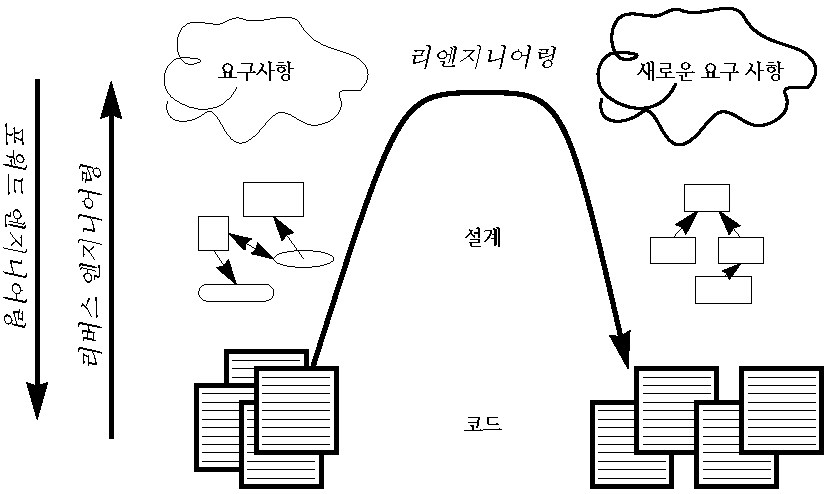
\includegraphics[width=\textwidth]{IntroLifecycle.pdf}
\caption{포워드 엔지니어링, 리버스 엔지니어링 그리고 리엔지니어링}
\figlabel{IntroLifecycle}
\end{center}
\end{figure}

\figref{IntroLifecycle}은 이 개념을 설명한다. \emph{포워드 엔지니어링(forward engineering)}은 높은 수준의 추상적인 모델과 아티팩트에서 구체적인 모델과 산출물로 이동하는 과정으로 이해할 수 있다. \emph{리버스 엔지니어링(reverse engineering)}은 코드에서 상위 수준의 모델과 산출물을 재구성한다. \emph{리엔지니어링(reengineering)}은 하나의 낮은 수준의 표현을 다른 표현으로 변환하는 과정이며, \emph{그 과정에서 상위 수준의 산출물을 다시 생성한다}. 

여기서 주목해야 할 핵심 사항은 리엔지니어링은 단순히 소스 코드를 변환하는 것이 아니라 시스템을 \emph{모든 수준}에서 변환하는 것이라는 점이다. 그렇기 때문에 리버스 엔지니어링과 리엔지니어링을 같은 맥락에서 이야기하는 것이 합리적이다. 일반적인 레거시 시스템에서는 소스 코드뿐만 아니라 모든 문서와 사양이 동기화되지 않은 것을 발견할 수 있다. 따라서 리버스 엔지니어링은 이해하지 못하는 것을 변형할 수 없기 때문에 리엔지니어링의 \emph{전제 조건(prerequisite)}이다.

%-----------------------------------------------------------------
\subsection*{리버스 엔지니어링}

무언가가 실제로 어떻게 작동하는지 이해하려고 할 때마다 \ind{리버스 엔지니어링(reverse engineering)}을 수행한다. 일반적으로 소프트웨어를 수정, 확장 또는 교체하려는 경우에만 리버스 엔지니어링이 필요하다. 소프트웨어를 리버스 엔지니어링해야 하는 이유는 때때로 \emph{사용 방법}을 이해하기 위해서일 수도 있다. 이는 리엔지니어링이 필요하다는 신호일 수도 있다. 따라서 리버스 엔지니어링 작업은 일반적으로 리엔지니어링에 대비해 소프트웨어를 \emph{재문서화(redocumenting)}하고 \emph{잠재적인 문제를 식별}하는 데 중점을 둔다.

리버스 엔지니어링을 하는 동안 다양한 정보 소스를 활용할 수 있다. 예를 들자면 다음과 같다.

\begin{bulletlist}

  \item 기존 문서 읽기

  \item 소스 코드 읽기

  \item 소프트웨어 실행해 보기

  \item 사용자 및 개발자 인터뷰하기

  \item 테스트 케이스 코딩 및 테스트 해보기

  \item 트레이스 생성 및 분석하기

  \item 다양한 도구로 소스 코드 및 트레이스의 하이 레벨 뷰(high-level views) 생성하기

  \item 버전 히스토리 분석하기
\end{bulletlist}

이러한 활동을 수행하면서 점진적으로 개선된 소프트웨어 모델을 구축하고, 다양한 질문과 답변을 찾고, 기술 문서를 정리하게 된다. 또한 수정해야 할 문제에 집중하게 될 것이다.

%-----------------------------------------------------------------
\subsection*{리엔지니어링}

시스템을 리엔지니어링하는 이유는 다양할 수 있지만, 실제 기술적인 문제는 일반적으로 매우 유사하다. 일반적으로 거시적인 아키텍처 문제와 세분화된 설계 문제가 혼합되어 있다. 대략적으로 문제를 분류해 보면 다음과 같다.

\begin{bulletlist}
  \item \emph{문서 부족(Insufficient documentation):}
  \index{문서!부족}
  문서가 존재하지 않거나 현실과 불일치한다.

  \item \emph{부적절한 레이어링(Improper layering):}
  \index{레이어링!부적절}
  누락되거나 부적절한 레이어링은 이식성(portability)과 적응성(adaptability)을 방해한다.

  \item \emph{모듈화 부족(Lack of modularity):}
  \index{모듈화!부족}
  모듈 간의 높은 결합도(couping)은 진화(evolution)를 방해한다.

  \item \emph{코드 중복(Duplicated code):}
  \index{코드 중복}
  ``복사, 붙여넣기 및 편집(copy, paste and edit)''은 빠르고 쉽지만 유지보수의 악몽(maintenance nightmares)으로 이어진다.

  \item \emph{기능 중복(Duplicated functionality):}
  \index{기능 중복}
  유사한 기능이 여러 팀에 의해 재구현되어 코드 비대화(code bloat)로 이어진다.
\end{bulletlist}

객체 지향 소프트웨어에서 발생하는 세분화된 가장 일반적인 문제는 다음과 같다.

\begin{bulletlist}
  \item \emph{상속의 오용(Misuse of inheritance):}
  \index{상속!오용}
  for composition, code reuse rather than polymorphism
  컴포지션(composition)의 경우 다형성(polymorphism)이 아닌 코드 재사용(code reuse)

  \item \emph{상속 누락(Missing inheritance):}
  \index{상속!누락}
  중복 코드(duplicated code)와 case 문에서 동작 선택하기 

  \item \emph{잘못 위치한 오퍼레이션(Misplaced operations):}
  \index{잘못 위치한 오펴레이션}
  잘못된 응집력(cohesion)\,---\,클래스 내부가 아닌 외부의 오퍼레이션의 위치

  \item \emph{캡슐화 위반(Violation of encapsulation):}
  \seeindex{캡슐화 위반}{캡술화, 위반}
  \index{캡슐화!위반}
  명시적 형 변환, C++ ``friends'' . 

  \item \emph{클래스 남용(Class abuse):}
  \index{클래스 남용}
  낮은 응집력(cohesion)\,---\,클래스를 네임스페이스처럼 사용
\end{bulletlist}

마지막으로, 변경하거나 교체하려는 시스템의 모든 부분에 대한 테스트 케이스를 철저하게 개발하여 리엔지니어링 활동을 위한 코드 기반을 준비한다.

리엔지니어링에는 마찬가지로 여러 가지 상호 관련된 활동이 따른다. 물론 가장 중요한 것 중 하나는 시스템의 어떤 부분을 수리하고 어떤 부분을 교체해야 하는지 평가하는 것이다.

\index{치코프스키, 엘리엇}
\index{크로스, 제임스}
실제로 수행되는 코드 변환은 여러 가지 범주로 나뉜다. 치코프스키와 크로스에 따르면 다음과 같다.

\index{리스터럭처링!정의}
\begin{quotation}
\noindent
``\emph{리스터럭처링(Restructuring)}는 시스템의 외부 동작을 유지하면서 동일한 상대적 추상화 수준에서 한 표현 형식에서 다른 표현 형식으로 변환하는 것이다.''
\end{quotation}

리스트럭처링은 일반적으로 소스 코드 변환(예: 비정형 ``스파게티'' 코드에서 구조화된 코드 또는 ``고투리스(goto-less)'' 코드로 자동 변환)을 의미하지만 디자인 수준에서의 변환도 포함할 수 있다. 

\index{리팩터링!정의}
\emph{리팩토링(Refactoring)}은 객체 지향 맥락 내에서 리스트럭처링하는 것이다. 마틴 파울러는 이렇게 정의한다.

\index{파울러, 마틴}
\begin{quotation}
\noindent
``\emph{리팩터링(Refactoring)}은 코드의 외부 동작을 변경하지 않으면서 내부 구조를 개선하는 방식으로 소프트웨어 시스템을 변경하는 프로세스이다.''

\hfill --- 마틴 파울러, \cite{Fowl99a}
\end{quotation}

소프트웨어 ``리엔지니어링(reengineering)''과 소프트웨어 ``유지보수(maintenance)''의 차이를 구분하기 어려울 수 있다. \ind{IEEE}는 \ind{소프트웨어 유지보수}를 정의하기 위해 여러 가지 시도를 해왔으며, 여기에는 다음도 포함된다.

\index{소프트웨어 유지보수!정의}
\begin{quotation}
\noindent
``결함을 수정하거나 성능 또는 기타 속성을 개선하거나 변경된 환경에 맞게 제품을 조정하기 위해 납품 후 소프트웨어 제품을 수정하는 것''. 
\end{quotation}

대부분의 사람들은 '유지보수'는 일상적인 작업인 반면 '리엔지니어링'은 그림 1에서 볼 수 있듯이 시스템을 재구성하는 과감하고 대대적인 노력이라고 생각할 것이다.

그러나 리엔지니어링은 단지 삶의 한 방식이라고 주장하는 사람들도 있다. 조금 개발하고, 조금 리엔지니어링하고, 조금 더 개발하는 식으로 \cite{Beck00a}. 실제로 건강하고 유지 관리 가능한 소프트웨어 시스템을 확보하기 위해서는 \emph{지속적인} 리엔지니어링 문화가 필요하다는 개념을 뒷받침하는 좋은 증거가 있다.

\index{리엔지니어링!지속적인}
그러나 지속적인 리엔지니어링(continuous reengineering)은 아직 일반적인 실천법이 아니기 때문에 이 책에서는 주요 리엔지니어링 노력의 맥락에서 패턴을 제시한다. 그럼에도 불구하고 독자들은 여기서 소개하는 대부분의 기법이 소규모 반복(iteration)에서 리엔지니어링에도 적용될 수 있다는 점을 염두에 두어야 한다.

%=================================================================
\section{리엔지니어링 패턴}

\index{리엔지니어링 패턴}
\index{알렉산더, 크리스토퍼}
글의 형식으로서의 패턴은 건축가 크리스토퍼 알렉산더가 1977년 그의 획기적인 저서인 \emph{패턴 랭귀지(A Pattern Language)}에서 소개했다. 이 책에서 알렉산더와 그의 동료들은 방에서 건물과 도시에 이르기까지 다양한 종류의 물리적 구조물을 설계하는 체계적인 방법을 제시했다. 각 문제는 여러 가지 주요한 요구사항(force)을 해결하는 일반적인 해결책인 반복되는 \emph{패턴(patter)}의 형태를 제시했지만, 특정 상황에 따라 각 문제에 고유한 방식으로 적용되어야 한다. 각 패턴에서 제시된 실제 해법은 그다지 흥미롭지 않았고, 오히려 패턴이 전달하는 \emph{중요한 요구 사항(force)}과 \emph{트레이드오프(tradeoff)}에 대한 논의가 포함되어 있다.

패턴은 디자인 문제에 대한 반복적인 해결책을 문서화하는 방법으로 소프트웨어 커뮤니티에서 처음 채택되었다. 알렉산더의 패턴과 마찬가지로, 각 디자인 패턴에는 해결해야 할 여러 가지 주요한 요구사항과 패턴을 적용할 때 고려해야 할 여러 가지 트레이드오프가 포함되었다. 패턴은 전문가들이 사용하는 실제 기법뿐만 아니라 그 뒤에 숨은 동기와 근거를 전달하는 간결한 방법인 것으로 밝혀졌다. 이후 패턴은 디자인 이외의 소프트웨어 개발의 여러 측면, 특히 소프트웨어를 설계하고 개발하는 \emph{프로세스(process)}에 적용되었다.

리엔지니어링 프로세스는 다른 프로세스와 마찬가지로 많은 표준 기법이 등장했으며, 각 기법은 다양한 주요한 요구사항을 해결하고 많은 트레이드오프를 포함할 수 있다. 모범 사례를 전달하는 방법으로서의 패턴은 이러한 기법을 제시하고 논의하는 데 특히 적합하다. 

\엠프{리엔지니어링 패턴(reengineering patterns)}은 레거시 소프트웨어 수정에 관한 지식을 체계화하고 기록하여 문제를 진단하고 시스템의 추가 개발을 방해할 수 있는 약점을 파악하는 데 도움이 되며, 새로운 요구 사항에 더 적합한 솔루션을 찾는 데도 도움이 된다. \ind{리엔지니어링 패턴}은 모든 리엔지니어링 작업에서 참조할 수 있는 안정적인 전문 지식 단위로, 완전한 방법론을 제안하지 않고 프로세스를 설명하며 특정 도구를 ``판매''하려는 것보다는 적절한 도구를 제안한다. 

리버스 엔지니어링 및 리엔지니어링 패턴의 대부분은 소프트웨어 설계와 관련이 있다는 점에서 디자인 패턴과 표면적으로 유사하다. 그러나 디자인 패턴은 디자인 문제에 대한 특정 해결책을 선택하는 것과 관련이 있는 반면, 리엔지니어링 패턴은 \emph{기존 디자인을 발견(discovering an existing design)}하고, 어떤 \emph{문제(problem)}가 있는지 파악하고, 이러한 \emph{문제를 해결(reparing)}하는 것과 관련이 있다는 점에서 중요한 차이가 있다. 결과적으로 리엔지니어링 패턴은 순전히 주어진 디자인 구조보다는 \emph{발견과 변형의 프로세스(process of discovery and transformation)}와 더 관련이 있다. 이러한 이유로 이 책에 나오는 대부분의 패턴의 이름은 \patpgref{어뎁터}{Adapter} 또는 \patpgref{파사드}{Facade}와 같이 구조 지향적이기보다는 \patpgref{항상 실행 버전 보유하기}{AlwaysHaveARunningVersion}와 같이 프로세스 지향적이다. 

디자인 패턴이 반복되는 \emph{디자인(design)} 문제에 대한 해결책을 제시하는 반면, 리엔지니어링 패턴은 반복되는 \emph{리엔지니어링(reengineering)} 문제에 대한 해결책을 제시한다. 리엔지니어링 패턴으로 생성되는 산출물이 반드시 디자인일 필요는 없다. 리팩터링된 코드처럼 구체적일 수도 있고, 리버스 엔지니어링 패턴의 경우 시스템 작동 방식에 대한 인사이트처럼 추상적일 수도 있다.

좋은 리엔지니어링 패턴의 특징은 (a) 기존 시스템 상태와 비교하여 목표 산출물의 장점, 비용 및 결과를 명확하게 드러내는 것이지, 그 결과가 얼마나 우아한지가 \emph{아닌} 것이고, (b) 리엔지니어링 \emph{프로세스(process)}에 대한 설명, 즉 시스템의 한 상태에서 다른 상태로 이동하는 방법을 명확하게 설명하는 것이다.

리엔지니어링 패턴은 코드 리팩터링 그 이상을 포함한다. 리엔지니어링 패턴은 증상을 감지하는 것으로 시작하여 새로운 솔루션에 도달하기 위한 코드 리팩터링으로 끝나는 프로세스를 설명할 수 있다. 리팩터링은 이 프로세스의 마지막 단계에 불과하며, 새로운 솔루션을 구현하기 위해 코드를 자동 또는 반자동으로 수정하는 기술적 문제를 해결한다. 리엔지니어링 패턴에는 리팩터링의 일부가 아닌 다른 요소도 포함되는데, 리엔지니어가 직면하고 있는 제약 조건을 고려하여 증상의 맥락을 강조하고 리팩터링된 솔루션이 가져올 수 있는 변경의 영향에 대한 논의가 여기에 포함된다. 
%=================================================================
\section{리엔지니어링 패턴의 형식}

\begin{figure}
\begin{center}
\includegraphics[width=\textwidth]{IntroEg}
\caption{일반적인 리엔지니어링 패턴의 포맷}
\figlabel{IntroEg}
\end{center}
\end{figure}
(TODO: PNG 파일 처리 필요 혹은 현상태 유지)

\index{리엔지니어링 패턴!형식}
이 책에서 사용하는 형식(form)을 설명하는 간단한 패턴의 예가 \figref{IntroEg}에 나와 있다. 패턴마다 다른 종류의 문제를 다루기 때문에 실제 사용되는 형식은 패턴마다 약간 다를 수 있지만 일반적으로 같은 종류의 큰제목(heading)을 볼 수 있다.

패턴의 이름(name)은 잘 선택하면 패턴을 기억하기 쉽고 동료들과 토론하기 쉽게 한다. (''\patref{이해를 위한 리팩터링}{RefactorToUnderstand}을 하지 않으면 여기서 무슨 일이 일어나고 있는지 알 수 없을 것 같다.'') 의도(intent)는 패턴의 본질을 매우 간결하게 전달하고 현재 상황에 적용 가능한지 여부를 알려주어야 한다. 

많은 리엔지니어링 패턴은 코드 변환과 관련이 있으며, 이 경우 다이어그램을 사용하여 어떤 종류의 변환이 일어나는지 설명할 수 있다. 일반적으로 이러한 패턴에는 해결해야 할 문제를 감지하는 단계와 변환 전후의 상황을 보여주는 코드 조각이 추가로 포함된다.

%=================================================================
\section{리엔지니어링 패턴 지도}

\begin{figure}
\begin{center}
\includegraphics[width=\textwidth]{IntroMap}
\caption{리엔지니어링 패턴의 클러스터 지도}
\figlabel{IntroMap}
\end{center}
\end{figure}

이 책의 패턴은 앞서 제시한 리엔지니어링 라이프사이클(reengineering lifecycle)에 따라 정리되어 있다. 그림 3에서 이 책의 각 챕터가 라이프사이클에 따라 패턴의 클러스터로 표현된 것을 볼 수 있다. 이 다이어그램은 패턴이 순서대로 적용될 수 있음을 시사한다. 하지만 실제로는 리버스 엔지니어링과 리엔지니어링 작업을 반복할 가능성이 더 높다. 이 다이어그램은 '워터폴(Waterfall)' 라이프사이클이 단순한 것과 같은 의미에서 단순하다. 비록 순차적으로 수행되지 않고 반복적으로 수행된다는 것을 알고 있더라도 다양한 소프트웨어 엔지니어링 활동과 그 관계를 추적하는 데 유용한 방법이 될 수 있다.

\index{패턴!언어}
각 패턴 클러스터(cluster of patterns)는 공통의 문제 집합을 해결하기 위해 결합될 수 있는 관련 패턴의 집합인 간단한 ``패턴 언어(pattern language)''\,---\로 표시된다. 따라서 각 장은 일반적으로 해당 장의 패턴에 대한 개요와 맵으로 시작하여 패턴이 어떻게 연관될 수 있는지 제안한다.

\on{FIX -- need chapter links}

\charef{방향 설정}{SettingDirection}에는 리엔지니어링 노력의 초점을 어디에 맞출지 결정하고 진행 상황을 파악하는 데 도움이 되는 몇 가지 패턴이 포함되어 있다. \charef{첫 번째 접근}{FirstContact}은 레거시 시스템을 처음 접할 때 유용할 수 있는 패턴 집합으로 구성되어 있다. \charef{초기 이해}{InitialUnderstanding}는 주로 클래스 다이어그램의 형태로 레거시 시스템의 첫 번째 간단한 모델을 개발하는 데 도움이 된다. \charef{디테일한 모델 캡처}{DetailedModelCapture}는 시스템의 특정 구성 요소에 대한 보다 상세한 모델을 개발하는 데 도움이 된다.

\charef{테스트라는 생명보험}{TestsYourLifeInsurance}는 레거시 시스템을 이해하는 데 도움이 될 뿐만 아니라 리엔지니어링 작업에 대비하기 위해 테스트를 사용하는 데 중점을 둔다. \charef{마이그레이션 전략}{MigrationStrategies}은 리엔지니어링하는 동안 시스템을 계속 실행하고 새 시스템이 사용자에게 받아들여질 가능성을 높이는 데 도움이 된다. \charef{중복 코드 감지}{DetectingDuplicatedCode}는 다른 버전의 소프트웨어에서 코드를 복사하여 붙여넣거나 병합했을 수 있는 위치를 식별하는 데 도움이 될 수 있다. \charef{책임 재배포}{RedistributeResponsibilities}는 너무 많은 책임을 가진 클래스를 발견하고 리엔지니어링하는 데 도움이 된다. \charef{다형성 적용한 조건문 변환}{TransformConditionalsToPolymorphism}은 객체 지향 디자인이 시간이 지남에 따라 손상된 경우 책임을 재분배하는 데 도움이 된다.

%=============================================================
\ifx\wholebook\relax\else
   \bibliographystyle{alpha}
   \bibliography{scg}
   \end{document}
\fi
%=============================================================

%=================================================================
%:PART 2 -- Reverse Engineering
\part{리버스 엔지니어링}
% $Author: oscar $
% $Date: 2009-09-15 16:53:48 +0200 (Tue, 15 Sep 2009) $
% $Revision: 29111 $
%=================================================================
\ifx\wholebook\relax\else
% --------------------------------------------
% Lulu:
	\documentclass[a4paper,10pt,twoside]{book}
	\usepackage[
		papersize={6.13in,9.21in},
		hmargin={.815in,.815in},
		vmargin={.98in,.98in},
		ignoreheadfoot
	]{geometry}
  \usepackage[hangul]{kotex}
	% $Author: oscar $
% $Date: 2009-09-13 20:58:29 +0200 (Sun, 13 Sep 2009) $
% $Revision: 29070 $
%=============================================================
% NB: documentclass must be set in main document.
% Allows book to be generated in multiple formats.
%=============================================================
%:Packages
\usepackage[T1]{fontenc}  %%%%%really important to get the code directly in the text!
\usepackage{palatino}
\usepackage{ifthen}
\usepackage{graphicx}
\graphicspath{{figures/}}
\usepackage{xspace}
\usepackage{makeidx}
\usepackage{isodateo} % enable \isodate
\usepackage{amssymb,textcomp}
%=============================================================
%:More packages
%\usepackage[english]{babel}
%\usepackage{lmodern}
%\usepackage[scaled=0.85]{helvet}
%\usepackage{microtype}
%\usepackage{theorem}
%\usepackage{float}
%\usepackage{longtable}
%\usepackage[nottoc]{tocbibind}
%\usepackage{multicol}
%\usepackage{booktabs}	% book-style tables
%\usepackage{topcapt}	% enables \topcaption
%\usepackage{multirow}
%\usepackage{tabularx}
%\usepackage{alltt}
\usepackage[usenames,dvipsnames]{color}
%\usepackage[hang]{subfigure}\makeatletter\def\p@subfigure{\thefigure\,}\makeatother
%\usepackage{rotating}
%\usepackage{enumitem}	% apb: allows more control over tags in enumerations
%\usepackage{verbatim}     % for comment environment
%\usepackage{varioref}	% for page references that work
%\usepackage{needspace}
%\usepackage[newparttoc]{titlesec}
%\usepackage{titletoc}
%\usepackage{wrapfig}
\usepackage[
	colorlinks=true,
	linkcolor=black,
	urlcolor=black,
	citecolor=black
]{hyperref}   % should come last
%=============================================================
%:URL style
\makeatletter
\def\url@leostyle{%
  \@ifundefined{selectfont}{\def\UrlFont{\sf}}{\def\UrlFont{\sffamily}}}
\makeatother
\urlstyle{leo}
%=============================================================
%:Booleans
\newboolean{lulu}
\setboolean{lulu}{false}
\newcommand{\ifluluelse}[2]{\ifthenelse{\boolean{lulu}}{#1}{#2}}
%=============================================================
%:Editorial comment macros
\newcommand{\nnbb}[2]{
  \fbox{\bfseries\sffamily\scriptsize#1}
  {\sf\small$\blacktriangleright$\textit{#2}$\blacktriangleleft$}
}
\newcommand{\on}[1]{\nnbb{Oscar}{#1}}
\newcommand{\here}{\nnbb{CONTINUE}{HERE}}
%=============================================================
%:Abbreviation macros
\newcommand{\ie}{\emph{i.e.},\xspace}
\newcommand{\eg}{\emph{e.g.},\xspace}
\newcommand{\etc}{\emph{etc.}\xspace}
\newcommand{\etal}{\emph{et al.}\xspace}
\newcommand{\straightquote}{"}
\newcommand{\sba}{\url{SquareBracketAssociates.org}\xspace}
%=============================================================
%:Patterns
% \newcommand{\pattern}[2]{\newpage\section{{\sf #1}}\label{pat:#2}}
% \newcommand{\pattern}[2]{\newpage\index{#1 (Pattern)}\section{#1}\label{pat:#2}}
\newcommand{\pattern}[2]{\cleardoublepage\index{#1 (패턴)}\section{#1}\label{pat:#2}}
\newcommand{\thumbnail}[2]{\index{#1 (패턴)}\subsection{#1}\label{pat:#2}}
\newcommand{\thumblang}[2]{\index{#1 (패턴 랭귀지)}\subsection{#1}\label{pat:#2}}
\newcommand{\variant}[1]{{\emph{#1}}\xspace}
% \newcommand{\problem}[1]{\subsection*{Problem}\emph{#1}}
\newcommand{\intent}[1]{\paragraph{의도}\emph{#1}}
\newcommand{\problem}[1]{\paragraph{문제}\emph{#1}}
\newcommand{\solution}[1]{\paragraph{해결}\emph{#1}}
\newcommand{\discussion}[0]{\paragraph{토론}}
\newcommand{\cmd}[1]{{\tt #1}\xspace}
%=============================================================
%:Environments
\newenvironment{bulletlist}{\begin{itemize}\setlength{\itemsep}{0ex}}
{\end{itemize}}
%=============================================================
%:Cross reference macros
\newcommand{\chalabel}[1]{\label{cha:#1}}
\newcommand{\seclabel}[1]{\label{sec:#1}}
\newcommand{\figlabel}[1]{\label{fig:#1}}
\newcommand{\tablabel}[1]{\label{tab:#1}}
\newcommand{\rulelabel}[1]{\label{rule:#1}}
\newcommand{\eglabel}[1]{\label{eg:#1}}
\newcommand{\scrlabel}[1]{\label{scr:#1}}
\newcommand{\mthlabel}[1]{\label{mth:#1}}
\newcommand{\clslabel}[1]{\label{cls:#1}}
\newcommand{\faqlabel}[1]{\label{faq:#1}}
%\newcommand{\charef}[1]{Chapter~\ref{cha:#1}\xspace}
%\newcommand{\secref}[1]{Section~\ref{sec:#1}\xspace}
\newcommand{\figref}[1]{Figure~\ref{fig:#1}\xspace}
% \newcommand{\patpgref}[2]{\hyperref[pat:#2]{\sf #1} [p.~\pageref{pat:#2}]\xspace}
\newcommand{\patpgref}[2]{\index{#1 (Pattern)}\hyperref[pat:#2]{#1} [p.~\pageref{pat:#2}]\xspace}
\newcommand{\patlangpgref}[2]{\index{#1 (Pattern language)}\hyperref[pat:#2]{#1} [p.~\pageref{pat:#2}]\xspace}
% \newcommand{\patref}[2]{\hyperref[pat:#2]{\sf #1}\xspace}
\newcommand{\patref}[2]{\index{#1 (Pattern)}\hyperref[pat:#2]{#1}\xspace}
\newcommand{\patlangref}[2]{\index{#1 (Pattern language)}\hyperref[pat:#2]{#1}\xspace}
% \newcommand{\charef}[2]{\hyperref[cha:#2]{\underline{\sf #1}}\xspace}
% \newcommand{\charef}[2]{\hyperref[cha:#2]{\sf #1}\xspace}
\newcommand{\charef}[2]{\index{#1 (Pattern cluster)}\hyperref[cha:#2]{#1}\xspace}
% \newcommand{\chapgref}[2]{\hyperref[cha:#2]{\sf #1} [p.~\pageref{cha:#2}]\xspace}
\newcommand{\chapgref}[2]{\index{#1 (Pattern cluster)}\hyperref[cha:#2]{#1} [p.~\pageref{cha:#2}]\xspace}
%\newcommand{\Figref}[1]{Figure~\ref{fig:#1}\xspace}
%\newcommand{\appref}[1]{Appendix~\ref{app:#1}\xspace}
%\newcommand{\tabref}[1]{Table~\ref{tab:#1}\xspace}
%\newcommand{\ruleref}[1]{\ref{rule:#1}\xspace}
%\newcommand{\egref}[1]{example~\ref{eg:#1}\xspace}
%\newcommand{\Egref}[1]{Example~\ref{eg:#1}\xspace}
%\newcommand{\scrref}[1]{script~\ref{scr:#1}\xspace}
%\newcommand{\Scrref}[1]{Script~\ref{scr:#1}\xspace}
%\newcommand{\tscrref}[1]{the script~\ref{scr:#1}\xspace}
%\newcommand{\Tscrref}[1]{The script~\ref{scr:#1}\xspace}
%\newcommand{\mthref}[1]{method~\ref{mth:#1}\xspace}
%\newcommand{\mthsref}[1]{methods~\ref{mth:#1}\xspace}
%\newcommand{\Mthref}[1]{Method~\ref{mth:#1}\xspace}
%\newcommand{\tmthref}[1]{the method~\ref{mth:#1}\xspace}
%\newcommand{\Tmthref}[1]{The method~\ref{mth:#1}\xspace}
%\newcommand{\clsref}[1]{class~\ref{cls:#1}\xspace}
%\newcommand{\tclsref}[1]{the class~\ref{cls:#1}\xspace}
%\newcommand{\Tclsref}[1]{The class~\ref{cls:#1}\xspace}
%=============================================================
%:Page Layout
\setlength{\headsep}{1cm}
%=============================================================
%:Menu item macro
%\definecolor{lightgray}{gray}{0.89}
%\newcommand{\menu}[1]{{%
%	\setlength{\fboxsep}{0pt}%
%	\colorbox{lightgray}{{{\upshape\sffamily\strut \,#1\,}}}}}
%\newcommand{\go}{\,$\triangleright$\,}
%\newcommand{\short}[1]{\mbox{{\sc cmd}\hspace{0.08em}--\hspace{0.09em}#1}\xspace}
%\newcommand{\button}[1]{{%
%	\setlength{\fboxsep}{0pt}%
%	\fbox{{\upshape\sffamily\strut \,#1\,}}}}
%\newcommand{\toolsflap}{\textit{Tools} flap\xspace}
%=============================================================
%:Section depth
%\setcounter{secnumdepth}{2}
%
%\DeclareGraphicsExtensions{.pdf, .jpg, .png}
%=============================================================
%:PDF setup
\hypersetup{
   pdftitle={Object-Oriented Reengineering Patterns},
   pdfauthor={Serge Demeyer, St\'ephane Ducasse, Oscar Nierstrasz},
   pdfkeywords={Reengineering, Object-Oriented Programming, Patterns},
   pdfsubject={Computer Science}
}
%=============================================================
%:Page layout and appearance
%\renewcommand{\chaptermark}[1]{\markboth{#1}{}}
%\renewcommand{\sectionmark}[1]{\markright{\thesection\ #1}}
%\renewpagestyle{plain}[\small\itshape]{%
%	\setheadrule{0pt}%
%	\sethead[][][]{}{}{}%
%	\setfoot[][][]{}{}{}}
%\renewpagestyle{headings}[\small\itshape]{%
%	\setheadrule{0pt}%
%	\setmarks{chapter}{section}%
%	\sethead[\thepage][][\chaptertitle]{\sectiontitle}{}{\thepage}%
%	\setfoot[][][]{}{}{}}
%=============================================================
%:Title section setup and TOC numbering depth
%\setcounter{secnumdepth}{1}
%\setcounter{tocdepth}{1}
%\titleformat{\part}[display]{\centering}{\huge\partname\ \thepart}{1em}{\Huge\textbf}[]
%\titleformat{\chapter}[display]{}{\huge\chaptertitlename\ \thechapter}{1em}{\Huge\raggedright\textbf}[]
%\titlecontents{part}[3pc]{%
%		\pagebreak[2]\addvspace{1em plus.4em minus.2em}%
%		\leavevmode\large\bfseries}
%	{\contentslabel{3pc}}{\hspace*{-3pc}}
%	{}[\nopagebreak]
%\titlecontents{chapter}[3pc]{%
%		\pagebreak[0]\addvspace{1em plus.2em minus.2em}%
%		\leavevmode\bfseries}
%	{\contentslabel{3pc}}{}
%	{\hfill\contentspage}[\nopagebreak]
%\dottedcontents{section}[3pc]{}{3pc}{1pc}
%\dottedcontents{subsection}[3pc]{}{0pc}{1pc}
%\let\origdoublepage\cleardoublepage
%\newcommand{\clearemptydoublepage}{%
%  \clearpage
%  {\pagestyle{empty}\origdoublepage}}
%\let\cleardoublepage\clearemptydoublepage % see http://www.tex.ac.uk/cgi-bin/texfaq2html?label=patch
%=============================================================
%:Listings package configuration
\newcommand{\caret}{\makebox{\raisebox{0.4ex}{\footnotesize{$\wedge$}}}}
% \newcommand{\escape}{{\sf \textbackslash}}
\definecolor{source}{gray}{0.95}
\usepackage{listings}
\lstdefinelanguage{Smalltalk}{
  morestring=[d]',
% Adapt this to other languages!
%  morecomment=[s]{"}{"},
  alsoletter={\#:},
  %escapechar={!},
  literate=
    {BANG}{!}1
%    {UNDERSCORE}{\_}1
    {\\st}{Smalltalk}9 % convenience -- in case \st occurs in code
    % {'}{{\textquotesingle}}1 % replaced by upquote=true in \lstset
%    {_}{{$\leftarrow$}}1
    {>>>}{{\sep}}1
    {^}{{$\uparrow$}}1
    {~}{{$\sim$}}1
    {-}{{\sf -\hspace{-0.13em}-}}1  % the goal is to make - the same width as +
    {+}{\raisebox{0.08ex}{+}}1		% and to raise + off the baseline to match -
    {-->}{{\quad$\longrightarrow$\quad}}3
	, % Don't forget the comma at the end!
  tabsize=4
}[keywords,comments,strings]

\lstset{language=Smalltalk,
	basicstyle=\sffamily,
	keywordstyle=\color{black}\bfseries,
	% stringstyle=\ttfamily, % Ugly! do we really want this? -- on
	mathescape=true,
	showstringspaces=false,
	keepspaces=true,
	breaklines=true,
	breakautoindent=true,
	backgroundcolor=\color{source},
	lineskip={-1pt}, % Ugly hack
	upquote=true, % straight quote; requires textcomp package
	columns=fullflexible} % no fixed width fonts
% \newcommand{\ct}{\lstinline[mathescape=false,basicstyle={\sffamily\upshape}]}
\newcommand{\ct}{\lstinline[mathescape=false,backgroundcolor=\color{white},basicstyle={\sffamily\upshape}]}
\newcommand{\lct}[1]{{\textsf{\textup{#1}}}}
%\newcommand{\scat}[1]{\emph{\textsf{#1}}\xspace}
%\newcommand{\prot}[1]{\emph{\textsf{#1}}\xspace}
% NB: No argument!
\lstnewenvironment{code}[0]{%
	\lstset{%
		% frame=lines,
		frame=single,
		framerule=0pt,
		mathescape=false
	}
}{}
%\def\ignoredollar#1{}
%=============================================================
%:Reserving space
%\newcommand{\needlines}[1]{\Needspace{#1\baselineskip}}
%=============================================================
%:Indexing macros
% Macros ending with "ind" generate text as well as an index entry
% Macros ending with "index" *only* generate an index entry
\newcommand{\ind}[1]{\index{#1}#1\xspace} % plain text
\newcommand{\subind}[2]{\index{#1!#2}#2\xspace} % show #2, subindex under #1
\newcommand{\emphind}[1]{\index{#1}\emph{#1}\xspace} % emph #1
\newcommand{\emphsubind}[2]{\index{#1!#2}\emph{#2}\xspace} % show emph #2, subindex under #1
\newcommand{\patind}[1]{\index{#1@#1 (pattern)}\ct{#1}\xspace} % pattern
\newcommand{\seeindex}[2]{\index{#1|see{#2}}} % #1, see #2
%\newcommand{\boldidx}[1]{{\bf #1}} % breaks hyperlink
%\newcommand{\indmain}[1]{\index{#1}#1\xspace} 
%\newcommand{\emphsubindmain}[2]{\index{#1!#2}\emph{#2}\xspace} % subindex, main entry
%\newcommand{\subindmain}[2]{\index{#1!#2}#2\xspace} % subindex, main entry
%\newcommand{\clsindmain}[1]{\index{#1!\#@(class)}\ct{#1}\xspace} % class main
%\newcommand{\indexmain}[1]{\index{#1}} 
%=============================================================
\parskip 1ex
%=============================================================

	\pagestyle{headings}
	\setboolean{lulu}{true}
% --------------------------------------------
% A4:
%	\documentclass[a4paper,11pt,twoside]{book}
%	% $Author: oscar $
% $Date: 2009-09-13 20:58:29 +0200 (Sun, 13 Sep 2009) $
% $Revision: 29070 $
%=============================================================
% NB: documentclass must be set in main document.
% Allows book to be generated in multiple formats.
%=============================================================
%:Packages
\usepackage[T1]{fontenc}  %%%%%really important to get the code directly in the text!
\usepackage{palatino}
\usepackage{ifthen}
\usepackage{graphicx}
\graphicspath{{figures/}}
\usepackage{xspace}
\usepackage{makeidx}
\usepackage{isodateo} % enable \isodate
\usepackage{amssymb,textcomp}
%=============================================================
%:More packages
%\usepackage[english]{babel}
%\usepackage{lmodern}
%\usepackage[scaled=0.85]{helvet}
%\usepackage{microtype}
%\usepackage{theorem}
%\usepackage{float}
%\usepackage{longtable}
%\usepackage[nottoc]{tocbibind}
%\usepackage{multicol}
%\usepackage{booktabs}	% book-style tables
%\usepackage{topcapt}	% enables \topcaption
%\usepackage{multirow}
%\usepackage{tabularx}
%\usepackage{alltt}
\usepackage[usenames,dvipsnames]{color}
%\usepackage[hang]{subfigure}\makeatletter\def\p@subfigure{\thefigure\,}\makeatother
%\usepackage{rotating}
%\usepackage{enumitem}	% apb: allows more control over tags in enumerations
%\usepackage{verbatim}     % for comment environment
%\usepackage{varioref}	% for page references that work
%\usepackage{needspace}
%\usepackage[newparttoc]{titlesec}
%\usepackage{titletoc}
%\usepackage{wrapfig}
\usepackage[
	colorlinks=true,
	linkcolor=black,
	urlcolor=black,
	citecolor=black
]{hyperref}   % should come last
%=============================================================
%:URL style
\makeatletter
\def\url@leostyle{%
  \@ifundefined{selectfont}{\def\UrlFont{\sf}}{\def\UrlFont{\sffamily}}}
\makeatother
\urlstyle{leo}
%=============================================================
%:Booleans
\newboolean{lulu}
\setboolean{lulu}{false}
\newcommand{\ifluluelse}[2]{\ifthenelse{\boolean{lulu}}{#1}{#2}}
%=============================================================
%:Editorial comment macros
\newcommand{\nnbb}[2]{
  \fbox{\bfseries\sffamily\scriptsize#1}
  {\sf\small$\blacktriangleright$\textit{#2}$\blacktriangleleft$}
}
\newcommand{\on}[1]{\nnbb{Oscar}{#1}}
\newcommand{\here}{\nnbb{CONTINUE}{HERE}}
%=============================================================
%:Abbreviation macros
\newcommand{\ie}{\emph{i.e.},\xspace}
\newcommand{\eg}{\emph{e.g.},\xspace}
\newcommand{\etc}{\emph{etc.}\xspace}
\newcommand{\etal}{\emph{et al.}\xspace}
\newcommand{\straightquote}{"}
\newcommand{\sba}{\url{SquareBracketAssociates.org}\xspace}
%=============================================================
%:Patterns
% \newcommand{\pattern}[2]{\newpage\section{{\sf #1}}\label{pat:#2}}
% \newcommand{\pattern}[2]{\newpage\index{#1 (Pattern)}\section{#1}\label{pat:#2}}
\newcommand{\pattern}[2]{\cleardoublepage\index{#1 (패턴)}\section{#1}\label{pat:#2}}
\newcommand{\thumbnail}[2]{\index{#1 (패턴)}\subsection{#1}\label{pat:#2}}
\newcommand{\thumblang}[2]{\index{#1 (패턴 랭귀지)}\subsection{#1}\label{pat:#2}}
\newcommand{\variant}[1]{{\emph{#1}}\xspace}
% \newcommand{\problem}[1]{\subsection*{Problem}\emph{#1}}
\newcommand{\intent}[1]{\paragraph{의도}\emph{#1}}
\newcommand{\problem}[1]{\paragraph{문제}\emph{#1}}
\newcommand{\solution}[1]{\paragraph{해결}\emph{#1}}
\newcommand{\discussion}[0]{\paragraph{토론}}
\newcommand{\cmd}[1]{{\tt #1}\xspace}
%=============================================================
%:Environments
\newenvironment{bulletlist}{\begin{itemize}\setlength{\itemsep}{0ex}}
{\end{itemize}}
%=============================================================
%:Cross reference macros
\newcommand{\chalabel}[1]{\label{cha:#1}}
\newcommand{\seclabel}[1]{\label{sec:#1}}
\newcommand{\figlabel}[1]{\label{fig:#1}}
\newcommand{\tablabel}[1]{\label{tab:#1}}
\newcommand{\rulelabel}[1]{\label{rule:#1}}
\newcommand{\eglabel}[1]{\label{eg:#1}}
\newcommand{\scrlabel}[1]{\label{scr:#1}}
\newcommand{\mthlabel}[1]{\label{mth:#1}}
\newcommand{\clslabel}[1]{\label{cls:#1}}
\newcommand{\faqlabel}[1]{\label{faq:#1}}
%\newcommand{\charef}[1]{Chapter~\ref{cha:#1}\xspace}
%\newcommand{\secref}[1]{Section~\ref{sec:#1}\xspace}
\newcommand{\figref}[1]{Figure~\ref{fig:#1}\xspace}
% \newcommand{\patpgref}[2]{\hyperref[pat:#2]{\sf #1} [p.~\pageref{pat:#2}]\xspace}
\newcommand{\patpgref}[2]{\index{#1 (Pattern)}\hyperref[pat:#2]{#1} [p.~\pageref{pat:#2}]\xspace}
\newcommand{\patlangpgref}[2]{\index{#1 (Pattern language)}\hyperref[pat:#2]{#1} [p.~\pageref{pat:#2}]\xspace}
% \newcommand{\patref}[2]{\hyperref[pat:#2]{\sf #1}\xspace}
\newcommand{\patref}[2]{\index{#1 (Pattern)}\hyperref[pat:#2]{#1}\xspace}
\newcommand{\patlangref}[2]{\index{#1 (Pattern language)}\hyperref[pat:#2]{#1}\xspace}
% \newcommand{\charef}[2]{\hyperref[cha:#2]{\underline{\sf #1}}\xspace}
% \newcommand{\charef}[2]{\hyperref[cha:#2]{\sf #1}\xspace}
\newcommand{\charef}[2]{\index{#1 (Pattern cluster)}\hyperref[cha:#2]{#1}\xspace}
% \newcommand{\chapgref}[2]{\hyperref[cha:#2]{\sf #1} [p.~\pageref{cha:#2}]\xspace}
\newcommand{\chapgref}[2]{\index{#1 (Pattern cluster)}\hyperref[cha:#2]{#1} [p.~\pageref{cha:#2}]\xspace}
%\newcommand{\Figref}[1]{Figure~\ref{fig:#1}\xspace}
%\newcommand{\appref}[1]{Appendix~\ref{app:#1}\xspace}
%\newcommand{\tabref}[1]{Table~\ref{tab:#1}\xspace}
%\newcommand{\ruleref}[1]{\ref{rule:#1}\xspace}
%\newcommand{\egref}[1]{example~\ref{eg:#1}\xspace}
%\newcommand{\Egref}[1]{Example~\ref{eg:#1}\xspace}
%\newcommand{\scrref}[1]{script~\ref{scr:#1}\xspace}
%\newcommand{\Scrref}[1]{Script~\ref{scr:#1}\xspace}
%\newcommand{\tscrref}[1]{the script~\ref{scr:#1}\xspace}
%\newcommand{\Tscrref}[1]{The script~\ref{scr:#1}\xspace}
%\newcommand{\mthref}[1]{method~\ref{mth:#1}\xspace}
%\newcommand{\mthsref}[1]{methods~\ref{mth:#1}\xspace}
%\newcommand{\Mthref}[1]{Method~\ref{mth:#1}\xspace}
%\newcommand{\tmthref}[1]{the method~\ref{mth:#1}\xspace}
%\newcommand{\Tmthref}[1]{The method~\ref{mth:#1}\xspace}
%\newcommand{\clsref}[1]{class~\ref{cls:#1}\xspace}
%\newcommand{\tclsref}[1]{the class~\ref{cls:#1}\xspace}
%\newcommand{\Tclsref}[1]{The class~\ref{cls:#1}\xspace}
%=============================================================
%:Page Layout
\setlength{\headsep}{1cm}
%=============================================================
%:Menu item macro
%\definecolor{lightgray}{gray}{0.89}
%\newcommand{\menu}[1]{{%
%	\setlength{\fboxsep}{0pt}%
%	\colorbox{lightgray}{{{\upshape\sffamily\strut \,#1\,}}}}}
%\newcommand{\go}{\,$\triangleright$\,}
%\newcommand{\short}[1]{\mbox{{\sc cmd}\hspace{0.08em}--\hspace{0.09em}#1}\xspace}
%\newcommand{\button}[1]{{%
%	\setlength{\fboxsep}{0pt}%
%	\fbox{{\upshape\sffamily\strut \,#1\,}}}}
%\newcommand{\toolsflap}{\textit{Tools} flap\xspace}
%=============================================================
%:Section depth
%\setcounter{secnumdepth}{2}
%
%\DeclareGraphicsExtensions{.pdf, .jpg, .png}
%=============================================================
%:PDF setup
\hypersetup{
   pdftitle={Object-Oriented Reengineering Patterns},
   pdfauthor={Serge Demeyer, St\'ephane Ducasse, Oscar Nierstrasz},
   pdfkeywords={Reengineering, Object-Oriented Programming, Patterns},
   pdfsubject={Computer Science}
}
%=============================================================
%:Page layout and appearance
%\renewcommand{\chaptermark}[1]{\markboth{#1}{}}
%\renewcommand{\sectionmark}[1]{\markright{\thesection\ #1}}
%\renewpagestyle{plain}[\small\itshape]{%
%	\setheadrule{0pt}%
%	\sethead[][][]{}{}{}%
%	\setfoot[][][]{}{}{}}
%\renewpagestyle{headings}[\small\itshape]{%
%	\setheadrule{0pt}%
%	\setmarks{chapter}{section}%
%	\sethead[\thepage][][\chaptertitle]{\sectiontitle}{}{\thepage}%
%	\setfoot[][][]{}{}{}}
%=============================================================
%:Title section setup and TOC numbering depth
%\setcounter{secnumdepth}{1}
%\setcounter{tocdepth}{1}
%\titleformat{\part}[display]{\centering}{\huge\partname\ \thepart}{1em}{\Huge\textbf}[]
%\titleformat{\chapter}[display]{}{\huge\chaptertitlename\ \thechapter}{1em}{\Huge\raggedright\textbf}[]
%\titlecontents{part}[3pc]{%
%		\pagebreak[2]\addvspace{1em plus.4em minus.2em}%
%		\leavevmode\large\bfseries}
%	{\contentslabel{3pc}}{\hspace*{-3pc}}
%	{}[\nopagebreak]
%\titlecontents{chapter}[3pc]{%
%		\pagebreak[0]\addvspace{1em plus.2em minus.2em}%
%		\leavevmode\bfseries}
%	{\contentslabel{3pc}}{}
%	{\hfill\contentspage}[\nopagebreak]
%\dottedcontents{section}[3pc]{}{3pc}{1pc}
%\dottedcontents{subsection}[3pc]{}{0pc}{1pc}
%\let\origdoublepage\cleardoublepage
%\newcommand{\clearemptydoublepage}{%
%  \clearpage
%  {\pagestyle{empty}\origdoublepage}}
%\let\cleardoublepage\clearemptydoublepage % see http://www.tex.ac.uk/cgi-bin/texfaq2html?label=patch
%=============================================================
%:Listings package configuration
\newcommand{\caret}{\makebox{\raisebox{0.4ex}{\footnotesize{$\wedge$}}}}
% \newcommand{\escape}{{\sf \textbackslash}}
\definecolor{source}{gray}{0.95}
\usepackage{listings}
\lstdefinelanguage{Smalltalk}{
  morestring=[d]',
% Adapt this to other languages!
%  morecomment=[s]{"}{"},
  alsoletter={\#:},
  %escapechar={!},
  literate=
    {BANG}{!}1
%    {UNDERSCORE}{\_}1
    {\\st}{Smalltalk}9 % convenience -- in case \st occurs in code
    % {'}{{\textquotesingle}}1 % replaced by upquote=true in \lstset
%    {_}{{$\leftarrow$}}1
    {>>>}{{\sep}}1
    {^}{{$\uparrow$}}1
    {~}{{$\sim$}}1
    {-}{{\sf -\hspace{-0.13em}-}}1  % the goal is to make - the same width as +
    {+}{\raisebox{0.08ex}{+}}1		% and to raise + off the baseline to match -
    {-->}{{\quad$\longrightarrow$\quad}}3
	, % Don't forget the comma at the end!
  tabsize=4
}[keywords,comments,strings]

\lstset{language=Smalltalk,
	basicstyle=\sffamily,
	keywordstyle=\color{black}\bfseries,
	% stringstyle=\ttfamily, % Ugly! do we really want this? -- on
	mathescape=true,
	showstringspaces=false,
	keepspaces=true,
	breaklines=true,
	breakautoindent=true,
	backgroundcolor=\color{source},
	lineskip={-1pt}, % Ugly hack
	upquote=true, % straight quote; requires textcomp package
	columns=fullflexible} % no fixed width fonts
% \newcommand{\ct}{\lstinline[mathescape=false,basicstyle={\sffamily\upshape}]}
\newcommand{\ct}{\lstinline[mathescape=false,backgroundcolor=\color{white},basicstyle={\sffamily\upshape}]}
\newcommand{\lct}[1]{{\textsf{\textup{#1}}}}
%\newcommand{\scat}[1]{\emph{\textsf{#1}}\xspace}
%\newcommand{\prot}[1]{\emph{\textsf{#1}}\xspace}
% NB: No argument!
\lstnewenvironment{code}[0]{%
	\lstset{%
		% frame=lines,
		frame=single,
		framerule=0pt,
		mathescape=false
	}
}{}
%\def\ignoredollar#1{}
%=============================================================
%:Reserving space
%\newcommand{\needlines}[1]{\Needspace{#1\baselineskip}}
%=============================================================
%:Indexing macros
% Macros ending with "ind" generate text as well as an index entry
% Macros ending with "index" *only* generate an index entry
\newcommand{\ind}[1]{\index{#1}#1\xspace} % plain text
\newcommand{\subind}[2]{\index{#1!#2}#2\xspace} % show #2, subindex under #1
\newcommand{\emphind}[1]{\index{#1}\emph{#1}\xspace} % emph #1
\newcommand{\emphsubind}[2]{\index{#1!#2}\emph{#2}\xspace} % show emph #2, subindex under #1
\newcommand{\patind}[1]{\index{#1@#1 (pattern)}\ct{#1}\xspace} % pattern
\newcommand{\seeindex}[2]{\index{#1|see{#2}}} % #1, see #2
%\newcommand{\boldidx}[1]{{\bf #1}} % breaks hyperlink
%\newcommand{\indmain}[1]{\index{#1}#1\xspace} 
%\newcommand{\emphsubindmain}[2]{\index{#1!#2}\emph{#2}\xspace} % subindex, main entry
%\newcommand{\subindmain}[2]{\index{#1!#2}#2\xspace} % subindex, main entry
%\newcommand{\clsindmain}[1]{\index{#1!\#@(class)}\ct{#1}\xspace} % class main
%\newcommand{\indexmain}[1]{\index{#1}} 
%=============================================================
\parskip 1ex
%=============================================================

%	\usepackage{a4wide}
% --------------------------------------------
	\begin{document}
	\renewcommand{\nnbb}[2]{} % Disable editorial comments
	\sloppy
\fi
%=================================================================
\chapter{방향 설정}
\chalabel{SettingDirection}

리엔지니어링 프로젝트를 시작하면 경영진, 사용자, 자신의 팀 등 다양한 측면에서 영향을 받는다. 기술적으로 가장 흥미로운 부분이나 가장 쉽게 고칠 수 있을 것 같은 부분에 집중하고 싶은 유혹에 빠지기 쉽다. 하지만 최선의 전략은 무엇일까? 리엔지니어링 작업의 방향을 어떻게 설정하고, 일단 시작한 후에는 어떻게 방향을 유지할까?

%-----------------------------------------------------------------
\subsection*{주요 요구 사항\footnote{force를 주요 요구 사항으로 번역하였다. -옮긴이}}
\begin{bulletlist}
  \item 일반적인 리엔지니어링 프로젝트에는 서로 다른 방향을 가지는 많은 이해관계가 얽혀 있다. 기술적, 인체공학적, 경제적, 정치적 고려 사항으로 인해 여러분과 여러분의 팀은 집중력을 확립하고 유지하기가 어려울 것이다. 

  \item 리엔지니어링 프로젝트의 커뮤니케이션은 기존 프로젝트의 개발팀의 유무에 따라 복잡해질 수 있다.

  \item 레거시 시스템은 시스템의 미래에 최선이 아닐 수 있는 특정 \ind{아키텍처(architecture)}로 사용자에게 강요할 수 있다.

  \item 레거시 소프트웨어에서 많은 문제를 발견할 수 있으며 우선순위를 설정하기가 어려울 것이다.

  \item 프로젝트에 가장 적합한 것이 아니라 가장 관심 있는 기술적 문제에 집중하는 유혹에 빠지기 쉽다.

  \item 레거시 시스템의 문제가 있는 구성 요소를 래핑(wrapping)할지, 리팩터링(refactoring)할지, 다시 작성(rewrite)할지 결정하기 어려울 수 있다. 이러한 각 옵션은 서로 다른 위험을 해결하며 필요한 노력, 결과를 평가할 수 있는 속도, 향후 수용할 수 있는 변경 사항의 종류에 따라 다른 결과를 가져온다.

  \item 시스템을 재설계할 때 가능한 모든 상황에 대처하기 위해 새 솔루션을 과도하게 설계(over-engineer)하고 싶은 유혹을 받을 수 있다.
\end{bulletlist}

\begin{figure}
\begin{center}
\includegraphics[width=\textwidth]{SettingDirectionMap}
\caption{리엔지니어링 프로젝트에서 방향을 설정하고 유지하기 위한 원칙과 지침}
\figlabel{SettingDirectionMap}
\end{center}
\end{figure}

%-----------------------------------------------------------------
\subsection*{Overview}

\charef{방향 설정}{SettingDirection}은 모든 개발 프로젝트에 적용할 수 있지만 리엔지니어링 작업과 특별한 관련성이 있는 패턴의 클러스터이다. 따라서 이를 설명하기 위해 문제(Problem), 해결책(Solution) 및 토론(Discussion)를 가지는 \emph{간결한 패턴 형식(streamlined pattern format)}을 선택했습니다.

리엔지니어링 팀 내에서 무엇이 문제이고 어떻게 달성할 수 있는지에 대한 공통된 이해를 확립하기 위해 \patref{맥심에 동의하기}{AgreeOnMaxims}를 작성해야 한다. 아키텍처 비전을 유지하기 위해 \patref{내비게이터 지정하기}{AppointANavigator}를 수행해야 한다. 모두가 \patref{라운드 테이블에 말하기}{SpeakToTheRoundTable}를 통해 프로젝트 상태에 대한 팀 인식을 유지해야 한다.

올바른 문제와 중요한 결정에 집중할 수 있도록 \patref{가장 가치 있는 것 먼저}{MostValuableFirst}를 사용하는 것이 현명하다. 이렇게 하면 \patref{사용자 참여시키기}{InvolveTheUsers} 및 \patref{자신감 만들기}{BuildConfidence}에 도움이 된다는 점에 참고하자. 래핑, 리팩터링 또는 재작성 여부를 결정하려면 \patref{증상이 아닌 문제 수정}{FixProblemsNotSymptoms}를 사용해야 한다. 변경을 위한 변경은 생산적이지 않으므로 \patref{고장이 나지 않으면 수정하지 않기}{IfItAintBrokeDontFixIt}를 사용하자. 새 시스템을 매우 유연하고 범용적으로 만들고 싶은 유혹이 있을 수 있지만, 거의 항상 \patref{단순함 유지하기}{KeepItSimple}을 사용하는 것이 더 좋다.

%=================================================================
%:PATTERN -- Agree on Maxims
\pattern{맥심에 동의하기}{AgreeOnMaxims}

\problem{팀에서 공통의 목적 의식(purpose)을 확립하려면 어떻게 해야 하는가?}

\solution{프로젝트의 핵심 우선순위를 정하고 팀이 궤도에 오르는 데 도움이 될 지침 원칙을 파악하자.}

\discussion
모든 리엔지니어링 프로젝트는 상충되는 수많은 이해관계에 대처해야 한다. 경영진은 제품의 경쟁력을 개선하고 유지보수 비용을 줄임으로써 레거시를 보호하고자 한다. 사용자는 기존 업무 패턴을 방해하지 않으면서 향상된 기능을 원한다. 개발자와 유지 관리자는 업무가 더 단순해지기를 원한다. 팀원들은 새로운 시스템의 모습에 대해 각자의 아이디어를 가지고 있을 수 있다.

\index{골드버그, 아델}
\index{루빈, 케니}
\emph{우리의 \ind{비즈니스 모델}(business model)은 무엇인가?} 또는 \emph{누가 무엇을 책임지는가?}와 같은 근본적인 질문에 대한 명확한 이해가 없다면 이해관계가 상충되어 팀이 분열되고 목표를 달성하지 못할 위험이 있다. 맥심(Maxim)은 여러 방향으로 끌려가는 프로젝트를 이끄는 데 도움이 되는 행동 규칙이다. 골드버그와 루빈은 \cite{Gold95a}에서 \emph{``모두가 테스트와 디버깅에 책임이 있다''}, \emph{``처음부터 제대로 할 수는 없다''} 등 수많은 \ind{맥심}의 예를 제시한다.

이 장의 모든 패턴은 팀을 안내하고 궤도에 맞추기 위한 것이므로 패턴이라기보다는 맥심(maxim)\footnote{행동에 본보기가 될 내용을 담고 있는 짧은 격언-옮긴이}으로 읽을 수 있다. 예를 들어 \patref{가장 가치 있는 것을 먼저}{MostValuableFirst}와 같은 맥심은 팀이 기술적으로는 흥미롭지만 레거시 시스템을 보호하거나 가치를 더하지 않는 한계적인 측면에 리엔지니어링 노력을 낭비하지 않도록 하기 위한 것이다. \patref{맥심에 동의하기}{AgreeOnMaxims}는 그 자체가 격언이므로 팀이 언제 방향타가 없는지 감지하는 데 도움이 될 수 있다.

기억해야 할 핵심 사항은 맥심의 수명이 제한적일 수 있다는 점이다. 채택된 맥심의 유효성을 주기적으로 재평가하는 것이 중요하다. 잘못된 맥심에 동의하거나 올바른 맥심에 동의하지만 시기가 잘못되면 프로젝트가 완전히 궤도에서 벗어날 수 있다.

%=================================================================
%:PATTERN -- Appoint a Navigator
\pattern{내비게이터 지정}{AppointANavigator}

\problem{복잡한 프로젝트 진행 중에 아키텍처 비전을 어떻게 유지하는가?}

\solution{아키텍처 비전이 유지될 수 있도록 내비게이터 역할을 담당할 사람을 지정하자.}

\discussion
모든 시스템의 \ind{아키텍처}는 시간이 지남에 따라 새로운 요구 사항과 관련성이 떨어지면서 성능이 저하되는 경향이 있다. 리엔지니어링 프로젝트의 과제는 레거시 시스템을 몇 년 더 지속하고 발전시킬 수 있는 새로운 아키텍처 비전을 개발하는 것이다. 내비게이터가 없으면 기존 시스템의 설계와 아키텍처가 새 시스템에 스며들어 그대로 이어지게 된다.

새로운 아키텍처가 해결해야 할 가장 중요한 문제가 무엇인지 결정하고 리엔지니어링 프로젝트 초기에 이러한 측면을 테스트할 수 있도록 \patref{가장 가치 있는 것을 먼저}{MostValuableFirst}를 해결해야 한다.

건전한 아키텍처는 \patref{증상이 아닌 문제 수정}{FixProblemsNotSymptoms}에 도움이 된다.

앨런 오캘러핸은 내비게이터를 ``불꽃의 수호자(Keeper of the Flame)''라고 부르기도 한다 \cite{Ocal99a}.

%=================================================================
%:PATTERN -- Speak to the Round Table
\pattern{원탁 회의에 말하기}{SpeakToTheRoundTable}

\problem{팀 소통의 동기화를 어떻게 유지하는가?}

\solution{간단하고 정기적인 원탁 회의를 개최하자.}

\discussion
레거시 시스템에 대한 지식과 이해는 항상 분산되어 있으며 대개 숨겨져 있다. 리엔지니어링 팀도 고고학을 수행하고 있다. 레거시 시스템에서 추출된 정보는 이를 활용하기 위해 반드시 공유해야 하는 귀중한 자산이다.

누구도 \ind{회의(meeting)}를 할 시간이 없지만, 회의가 없으면 커뮤니케이션은 임시방편적이고 무작위로 이루어진다. 정기적이고 집중적인 원탁 회의는 팀원들이 현재 상황에 대한 정보를 공유할 수 있도록 하는 목표를 달성할 수 있다. 원탁 회의는 짧게 진행하되 모든 사람이 참여해야 한다. 간단한 접근 방식은 모든 사람이 지난 회의 이후 무엇을 했는지, 무엇을 배웠는지, 또는 어떤 문제가 발생했는지, 다음 회의까지 무엇을 할 계획인지 말하도록 하는 것이다.

원탁 회의는 적어도 일주일에 한 번, 많게는 매일 개최하는 것이 좋다.

회의록은 진행 상황을 기록하는 데 중요하지만 회의록을 작성하는 것은 귀찮은 일이 될 수 있다. 회의록을 간단하게 작성하려면 특정 기한(deadline)까지 수행해야 할 \emph{결정사항(decisions)} 및 \emph{조치사항(actions)}만 기록하자.

\index{벡, 켄트}
\index{파울러, 마틴}
벡과 파울러는 원탁 회의를 짧게 진행하는 방법으로 ``스탠드업 미팅(Stand Up Meetings)''(의자 없는 회의)을 추천한다 \cite{Beck01a}.

%=================================================================
%:PATTERN -- Most Valuable First
\pattern{가장 가치 있는 것 먼저 하기}{MostValuableFirst}

\problem{어떤 문제에 먼저 집중해야 할까?}

\solution{고객에게 가장 가치 있는 측면부터 작업을 시작하자.}

\discussion
레거시 시스템에는 수많은 문제가 있을 수 있으며, 그 중에는 중요한 문제도 있고 고객의 비즈니스에 전혀 중요하지 않은 문제도 있을 수 있다. 가장 중요한 부분에 먼저 집중하면 문제가 되는 올바른 문제를 파악할 가능성이 높아지며, 마이그레이션할 \ind{아키텍처} 또는 새 시스템에 어떤 종류의 유연성을 구축할지 등 가장 중요한 결정을 프로젝트 초기에 테스트할 수 있다.

고객에게 가치 있는 시스템 부분에 먼저 집중함으로써 여러분과 팀원, 고객이 프로젝트에 대해 최대한 헌신할 수 있게 한다. 또한 리엔지니어링 노력이 가치 있고 필요하다는 것을 입증하는 긍정적인 결과를 조기에 얻을 가능성이 높아진다.

그럼에도 불구하고 이 패턴을 적용하는 데는 여러 가지 어려움이 있다.

\emph{고객은 누구인가?}

\index{이해관계자}
\begin{bulletlist}
  \item 모든 레거시 시스템에는 많은 이해관계자가 있지만 그 중 단 하나만 고른다면 고객이다. 누가 결정권을 가져야 하는지 명확하게 이해한 경우에만 우선순위를 설정할 수 있다.
\end{bulletlist}

\emph{무엇이 가치 있는 일인지 어떻게 알 수 있을까?}

\begin{bulletlist}
  \item 고객에게 가장 가치 있는 측면이 무엇인지 정확히 평가하는 것은 어려울 수 있다. 한 회사에서 아키텍처를 바꾸고 싶어서 시스템을 모듈화할 수 있는지 평가해 달라고 요청한 적이 있다. 하지만 오랜 논의 끝에 실제로는 비즈니스 규칙을 더 명확하게 표현할 수 있는 시스템이 필요하다는 것, 즉 한 명의 프로그래머만 이해하는 위험을 줄이기 위해 신입 프로그래머라도 더 쉽게 이해할 수 있는 시스템을 원한다는 것이 밝혀졌었다.

  \item 고객의 비즈니스 모델을 이해하려고 노력하라. 이를 통해 시스템의 다양한 측면의 가치를 평가하는 방법을 알 수 있다. 비즈니스 모델과 직접 관련이 없는 모든 것은 순전히 기술적인 측면의 문제일 가능성이 높다. 

  \item 고객이 얻고자 하는  \emph{측정 가능한 목표}가 무엇인지 파악하라. 예를 들어 응답 시간 개선, 새로운 기능의 출시 시간 단축, 개별 고객의 요구에 더 쉽게 맞춤화 등 시스템의 일부 측면 또는 시스템의 진화에 대한 외형적 표현이어야 한다.

  \item 주요 목표가 주로 \emph{기존 자산을 보호하는 것}인지, 아니면 새로운 기능이나 기능의 측면에서 \emph{가치를 추가하는 것}인지 이해하려고 노력하라.

  \item 변경 로그를 살펴보고 시스템에서 시간상으로 가장 많은 변경 활동이 있었던 위치를 파악하라. 가장 가치 있는 산출물(artifact)는 대개 가장 많은 변경 요청을 받은 산출물이다(\patpgref{과거로부터 학습}{LearnFromThePast} 참조). 

  \item 고객이 우선순위를 설정할 의향이 없거나 설정할 수 없는 경우에는 \emphind{계획 세우기 게임}(Planning Game)을 수행하자\cite{Beck01a}. 모든 이해관계자로부터 요구사항을 수집하고 식별 가능한 각 작업에 필요한 노력에 대한 대략적인 추정치를 만든다. 초기 첫 번째 마일스톤에 대한 초기 노력 예산이 주어지면 고객에게 예산에 맞는 작업을 선택하도록 요청한다. 각 반복(iteration)마다 이 플래닝 게임 적용을 실천한다.

  \item \emph{인식 변화(changing perceptions)}에 주의하라. 처음에는 고객이 문제 자체보다는 레거시 시스템에서 나타나는 특정 증상에 주목할 수 있다(\patpgref{증상이 아닌 문제 수정}{FixProblemsNotSymptoms} 참조). 
\end{bulletlist}

\emph{기대치가 너무 높아질 위험이 있지 않는가?}

\begin{bulletlist}
  \item 좋은 초기 결과를 제공하지 못하면 많은 것을 배울 수 있지만 신뢰도를 잃을 위험이 있다. 따라서 고객에게 가치를 제공할 뿐만 아니라 성공 가능성도 높은 초기 작업을 신중하게 선택하는 것이 중요하다. 따라서 초기 작업의 노력을 추정할 때 세심한 주의를 기울이자.

  \item 성공의 열쇠는 작고 빈번한 반복(iteration)을 계획하는 것이다. 고객이 파악한 초기 작업이 너무 커서 단기간(예: 2주)에 초기 결과를 보여줄 수 없다면 더 짧은 반복으로 해결할 수 있는 작은 하위 작업으로 세분화하자. 첫 단계에 성공하면 기대치가 높아지겠지만, 단계가 작아도 나쁘지 않다.
\end{bulletlist}

\emph{가장 가치 있는 부분이 쥐의 둥지(rat's nest)라면 어떨까?}

\begin{bulletlist}
  \item 안타깝게도 레거시 시스템을 리엔지니어링하는 것은 정상적이고 주기적인 혁신 프로세스가 아니라 절박한 상황에서 이루어지는 경우가 많다. 시스템에서 가장 중요한 부분이 가장 복잡하고 난공불락이며 수정과 디버깅이 어려운 부분일 수도 있다. 

  \item 높은 변경률(high changes rates)은 소프트웨어 결함이 많다는 신호일 수도 있다. 소프트웨어 결함의 80\%는 일반적으로 코드의 5\%에서 발생하므로 ``최악을 먼저 고친다''는 전략은 시스템에서 가장 심각한 문제의 원인을 제거함으로써 큰 성과를 거둘 수 있다 \cite{Davi95a}. 그럼에도 불구하고 상당한 위험이 따른다.

	\begin{bulletlist}
    \item 	조기에 긍정적인 결과를 입증하기 어려울 수 있다.
  
    \item 	정보가 거의 없는 상태에서 시스템의 가장 복잡한 부분을 다룰 수 있다.

    \item 	실패할 가능성이 높다.
	\end{bulletlist}

  \item 문제가 있는 구성 요소를 래핑할지, 리팩터링할지 또는 다시 작성할지 여부를 \patref{증상이 아닌 문제 수정}{FixProblemsNotSymptoms}를 확인하여 결정한다.

\end{bulletlist}

시스템에서 작업할 가장 중요한 부분이 무엇인지 결정한 후에는 리엔지니어링 노력에 \patpgref{사용자 참여시키기}{InvolveTheUsers}를 수행하여 \patpgref{신뢰 구축하기}{BuildConfidence}을 수행해야 한다. \patpgref{시스템 점진적 마이그레이션하기}{MigrateSystemsIncrementally}을 사용하면 사용자가 리엔지니어링된 시스템을 사용하면서 지속적인 피드백을 제공할 수 있다.

%=================================================================
%:PATTERN -- Fix Problems, Not Symptoms
\pattern{증상이 아닌 문제 수정하기}{FixProblemsNotSymptoms}

\problem{보고된 모든 문제를 어떻게 해결할 수 있을까?}

\solution{이해관계자의 요청이 아닌 문제의 원인을 해결하자.}

\discussion
이것은 매우 일반적인 원칙이지만 리엔지니어링과 특히 관련이 있다. \ind{이해관계자}\emph{(stakeholder)}마다 시스템에 대한 관점이 다르고 시스템의 일부만 볼 수도 있다. 그들이 고치기를 원하는 문제는 시스템의 더 깊은 문제를 드러내는 것일 수도 있다. 예를 들어 특정 사용자 작업에 대한 즉각적인 피드백을 받지 못하는 것은 데이터 흐름 아키텍처의 결과일 수 있다. 해결 방법을 구현하면 문제가 악화되어 더 많은 해결 방법이 필요할 수 있다. 이것이 진짜 문제라면 적절한 아키텍처로 마이그레이션해야 한다.

리엔지니어링 작업 중 흔히 발생하는 어려움은 레거시 컴포넌트를 래핑할지, 리팩터링할지, 다시 작성할지 결정하는 것이다. \patref{가장 가치 있는 것 먼저 하기}{MostValuableFirst}는 시스템의 문제에 어떤 우선순위를 부여할지 결정하는 데 도움이 되며, 어떤 문제가 중요한 경로에 있는지를 알려준다. \patref{증상이 아닌 문제 수정하기}{FixProblemsNotSymptoms}는 문제의 현상이 아닌 문제의 원인에 집중하도록 한다. 예를 들자면 다음과 같은 것들이 있다.

\begin{bulletlist}
  \item 레거시 컴포넌트의 코드가 기본적으로 안정적이고 문제가 주로 클라이언트 변경에서 발생하는 경우, 코드가 아무리 엉망이라도 구현이 아니라 레거시 컴포넌트에 대한 인터페이스에 문제가 있을 가능성이 높다. 이러한 경우 \patpgref{올바른 인터페이스 제공하기}{PresentTheRightInterface}를 적용하여 인터페이스만 수정하는 것을 고려해야 한다.

  \item 레거시 컴포넌트에 결함이 거의 없지만 시스템 변경에 큰 병목 현상이 발생하는 경우 향후 변경의 영향을 제한하기 위해 리팩터링해야 할 수도 있다. 보다 깔끔한 디자인으로 마이그레이션하기 위해 \patpgref {신 클래스 분할하기}{SplitUpGodClass}를 적용하는 것을 고려할 수 있다.

  \item 레거시 컴포넌트에 많은 결함이 있는 경우, 레거시 데이터를 새 구현으로 마이그레이션하기 위한 전략으로 \patpgref{새로운 마을로 다리 만들기}{MakeABridgeToTheNewTown}을 적용하는 것을 고려하자.
\end{bulletlist}

이 패턴은 \patref{고장이 나지 않으면 수정하지 않기}{IfItAintBrokeDontFixIt}과 충돌하는 것처럼 보일 수 있지만 실제로는 그렇지 않다. 실제로 '깨지지 않은' 것은 문제의 원인이 될 수 없다. 예를 들어 래핑은 해결 방법처럼 보일 수 있지만 실제 문제가 레거시 컴포넌트에 대한 인터페이스에만 있는 경우 올바른 해결책이 될 수 있다.

%=================================================================
%:PATTERN -- If It Ain't Broke, Don't Fix It
\pattern{고장이 나지 않으면 수정하지 않기}{IfItAintBrokeDontFixIt}

\problem{레거시 시스템에서 어떤 부분을 리엔지니어링하고 어떤 부분을 그대로 둬야 할까?}

\solution{``고장난'' 부분, 즉 계획된 변경에 더 이상 적용할 수 없는 부분만 수정하자.}

\discussion
변화를 위한 변화가 반드시 좋은 것만은 아니다. 레거시 시스템에는 보기 흉할 수 있지만 잘 작동하고 유지 관리에 큰 부담이 되지 않는 부분이 있을 수 있다. 이러한 구성 요소를 분리하고 포장할 수 있다면 교체할 필요가 없을 수도 있다.

무언가를 ``수정''할 때마다 시스템의 다른 무언가가 손상될 위험도 있다. 또한 사소한 문제에 귀중한 시간과 노력을 낭비할 위험도 있다.

리엔지니어링 프로젝트에서 ``고장난'' 부분은 레거시를 위험에 빠뜨리는 부분이다.
\begin{bulletlist}
  \item 새로운 요구 사항을 충족하기 위해 자주 조정해야 하지만 높은 복잡성과 디자인 드리프트(design drift)\footnote{설계와 구현의 차이-옮긴이}로 인해 수정하기 어려운 컴포넌트(component).
  
  \item 중요하지만 전통적으로 많은 결함을 포함하는 컴포넌트.
\end{bulletlist}

안정적이고 레거시 시스템의 미래를 위협하지 않는 소프트웨어 산출물은 코드가 어떤 상태에 있든 ``고장난'' 것이 아니므로 다시 엔지니어링할 필요가 없다.

%=================================================================
%:PATTERN -- Keep It Simple
\pattern{간단하게 유지 하기}{KeepItSimple}

\problem{새 시스템에 얼마나 많은 유연성을 구축해야 할까?}

\solution{더 일반적이고 복잡한 솔루션보다 적절하고 간단한 솔루션이 더 낮다.}

\discussion
이것은 리엔지니어링에 특별한 의미를 갖는 또 다른 일반적인 원칙이다. 우리는 실제로 얼마나 많은 일반성과 유연성이 필요한지 추측하는 데 서툴다. 많은 소프트웨어 시스템은 생각할 수 있는 모든 기능이 추가되면서 비대해진다.

유연성(flexibility)은 양날의 검입니다. 리엔지니어링의 중요한 목표는 미래의 변화를 수용하는 것이다. 하지만 지나친 유연성은 새로운 시스템을 너무 복잡하게 만들어 오히려 미래의 변화를 방해할 수 있다.

어떤 사람들은 ``재사용을 위한 계획(plan for reuse)''이 필요하므로 누군가에게 유용할 수 있는 모든 소프트웨어 개체가 가능한 한 많은 노브와 버튼으로 가능한 가장 일반적인 방식으로 프로그래밍되도록 추가적인 노력을 기울여야 한다고 주장한다. 하지만 누가 어떤 용도로 어떤 것을 사용할지 예측하는 것은 거의 불가능하기 때문에 이런 방식은 거의 효과가 없다. 최종 사용자 소프트웨어도 마찬가지이다.

\seeindex{XP}{익스트림 프로그래밍}
``\ind{일할 수 있는 가장 간단한 것을 하라}''는 \ind{익스트림 프로그래밍}의 맥심이다. \cite{Beck00a}의 맥심으로, 모든 리엔지니어링 노력에 적용된다. 이 전략은 사용자가 평가하고 대응할 수 있는 간단한 변경 사항을 신속하게 도입하도록 장려하기 때문에 \patpgref{사용자 참여 시키기}{InvolveTheUsers} 및 \patpgref{신뢰 구축 하기}{BuildConfidence}을 강화한다.

복잡한 작업을 수행하면 (실제로 필요한 것이 무엇인지) 잘못 추측할 수 있고 수정하기가 더 어려워진다. 일을 단순하게 유지하면 더 빨리 끝내고, 더 빨리 피드백을 받고, 더 쉽게 오류를 복구할 수 있다. 그런 다음 다음 단계로 넘어갈 수 있다.

%=============================================================
\ifx\wholebook\relax\else
   \bibliographystyle{alpha}
   \bibliography{scg}
   \end{document}
\fi
%=============================================================

% $Author: oscar $
% $Date: 2009-09-15 16:53:48 +0200 (Tue, 15 Sep 2009) $
% $Revision: 29111 $
%=================================================================
\ifx\wholebook\relax\else
% --------------------------------------------
% Lulu:
	\documentclass[a4paper,10pt,twoside]{book}
	\usepackage[
		papersize={6.13in,9.21in},
		hmargin={.815in,.815in},
		vmargin={.98in,.98in},
		ignoreheadfoot
	]{geometry}
  \usepackage[hangul]{kotex}
	% $Author: oscar $
% $Date: 2009-09-13 20:58:29 +0200 (Sun, 13 Sep 2009) $
% $Revision: 29070 $
%=============================================================
% NB: documentclass must be set in main document.
% Allows book to be generated in multiple formats.
%=============================================================
%:Packages
\usepackage[T1]{fontenc}  %%%%%really important to get the code directly in the text!
\usepackage{palatino}
\usepackage{ifthen}
\usepackage{graphicx}
\graphicspath{{figures/}}
\usepackage{xspace}
\usepackage{makeidx}
\usepackage{isodateo} % enable \isodate
\usepackage{amssymb,textcomp}
%=============================================================
%:More packages
%\usepackage[english]{babel}
%\usepackage{lmodern}
%\usepackage[scaled=0.85]{helvet}
%\usepackage{microtype}
%\usepackage{theorem}
%\usepackage{float}
%\usepackage{longtable}
%\usepackage[nottoc]{tocbibind}
%\usepackage{multicol}
%\usepackage{booktabs}	% book-style tables
%\usepackage{topcapt}	% enables \topcaption
%\usepackage{multirow}
%\usepackage{tabularx}
%\usepackage{alltt}
\usepackage[usenames,dvipsnames]{color}
%\usepackage[hang]{subfigure}\makeatletter\def\p@subfigure{\thefigure\,}\makeatother
%\usepackage{rotating}
%\usepackage{enumitem}	% apb: allows more control over tags in enumerations
%\usepackage{verbatim}     % for comment environment
%\usepackage{varioref}	% for page references that work
%\usepackage{needspace}
%\usepackage[newparttoc]{titlesec}
%\usepackage{titletoc}
%\usepackage{wrapfig}
\usepackage[
	colorlinks=true,
	linkcolor=black,
	urlcolor=black,
	citecolor=black
]{hyperref}   % should come last
%=============================================================
%:URL style
\makeatletter
\def\url@leostyle{%
  \@ifundefined{selectfont}{\def\UrlFont{\sf}}{\def\UrlFont{\sffamily}}}
\makeatother
\urlstyle{leo}
%=============================================================
%:Booleans
\newboolean{lulu}
\setboolean{lulu}{false}
\newcommand{\ifluluelse}[2]{\ifthenelse{\boolean{lulu}}{#1}{#2}}
%=============================================================
%:Editorial comment macros
\newcommand{\nnbb}[2]{
  \fbox{\bfseries\sffamily\scriptsize#1}
  {\sf\small$\blacktriangleright$\textit{#2}$\blacktriangleleft$}
}
\newcommand{\on}[1]{\nnbb{Oscar}{#1}}
\newcommand{\here}{\nnbb{CONTINUE}{HERE}}
%=============================================================
%:Abbreviation macros
\newcommand{\ie}{\emph{i.e.},\xspace}
\newcommand{\eg}{\emph{e.g.},\xspace}
\newcommand{\etc}{\emph{etc.}\xspace}
\newcommand{\etal}{\emph{et al.}\xspace}
\newcommand{\straightquote}{"}
\newcommand{\sba}{\url{SquareBracketAssociates.org}\xspace}
%=============================================================
%:Patterns
% \newcommand{\pattern}[2]{\newpage\section{{\sf #1}}\label{pat:#2}}
% \newcommand{\pattern}[2]{\newpage\index{#1 (Pattern)}\section{#1}\label{pat:#2}}
\newcommand{\pattern}[2]{\cleardoublepage\index{#1 (패턴)}\section{#1}\label{pat:#2}}
\newcommand{\thumbnail}[2]{\index{#1 (패턴)}\subsection{#1}\label{pat:#2}}
\newcommand{\thumblang}[2]{\index{#1 (패턴 랭귀지)}\subsection{#1}\label{pat:#2}}
\newcommand{\variant}[1]{{\emph{#1}}\xspace}
% \newcommand{\problem}[1]{\subsection*{Problem}\emph{#1}}
\newcommand{\intent}[1]{\paragraph{의도}\emph{#1}}
\newcommand{\problem}[1]{\paragraph{문제}\emph{#1}}
\newcommand{\solution}[1]{\paragraph{해결}\emph{#1}}
\newcommand{\discussion}[0]{\paragraph{토론}}
\newcommand{\cmd}[1]{{\tt #1}\xspace}
%=============================================================
%:Environments
\newenvironment{bulletlist}{\begin{itemize}\setlength{\itemsep}{0ex}}
{\end{itemize}}
%=============================================================
%:Cross reference macros
\newcommand{\chalabel}[1]{\label{cha:#1}}
\newcommand{\seclabel}[1]{\label{sec:#1}}
\newcommand{\figlabel}[1]{\label{fig:#1}}
\newcommand{\tablabel}[1]{\label{tab:#1}}
\newcommand{\rulelabel}[1]{\label{rule:#1}}
\newcommand{\eglabel}[1]{\label{eg:#1}}
\newcommand{\scrlabel}[1]{\label{scr:#1}}
\newcommand{\mthlabel}[1]{\label{mth:#1}}
\newcommand{\clslabel}[1]{\label{cls:#1}}
\newcommand{\faqlabel}[1]{\label{faq:#1}}
%\newcommand{\charef}[1]{Chapter~\ref{cha:#1}\xspace}
%\newcommand{\secref}[1]{Section~\ref{sec:#1}\xspace}
\newcommand{\figref}[1]{Figure~\ref{fig:#1}\xspace}
% \newcommand{\patpgref}[2]{\hyperref[pat:#2]{\sf #1} [p.~\pageref{pat:#2}]\xspace}
\newcommand{\patpgref}[2]{\index{#1 (Pattern)}\hyperref[pat:#2]{#1} [p.~\pageref{pat:#2}]\xspace}
\newcommand{\patlangpgref}[2]{\index{#1 (Pattern language)}\hyperref[pat:#2]{#1} [p.~\pageref{pat:#2}]\xspace}
% \newcommand{\patref}[2]{\hyperref[pat:#2]{\sf #1}\xspace}
\newcommand{\patref}[2]{\index{#1 (Pattern)}\hyperref[pat:#2]{#1}\xspace}
\newcommand{\patlangref}[2]{\index{#1 (Pattern language)}\hyperref[pat:#2]{#1}\xspace}
% \newcommand{\charef}[2]{\hyperref[cha:#2]{\underline{\sf #1}}\xspace}
% \newcommand{\charef}[2]{\hyperref[cha:#2]{\sf #1}\xspace}
\newcommand{\charef}[2]{\index{#1 (Pattern cluster)}\hyperref[cha:#2]{#1}\xspace}
% \newcommand{\chapgref}[2]{\hyperref[cha:#2]{\sf #1} [p.~\pageref{cha:#2}]\xspace}
\newcommand{\chapgref}[2]{\index{#1 (Pattern cluster)}\hyperref[cha:#2]{#1} [p.~\pageref{cha:#2}]\xspace}
%\newcommand{\Figref}[1]{Figure~\ref{fig:#1}\xspace}
%\newcommand{\appref}[1]{Appendix~\ref{app:#1}\xspace}
%\newcommand{\tabref}[1]{Table~\ref{tab:#1}\xspace}
%\newcommand{\ruleref}[1]{\ref{rule:#1}\xspace}
%\newcommand{\egref}[1]{example~\ref{eg:#1}\xspace}
%\newcommand{\Egref}[1]{Example~\ref{eg:#1}\xspace}
%\newcommand{\scrref}[1]{script~\ref{scr:#1}\xspace}
%\newcommand{\Scrref}[1]{Script~\ref{scr:#1}\xspace}
%\newcommand{\tscrref}[1]{the script~\ref{scr:#1}\xspace}
%\newcommand{\Tscrref}[1]{The script~\ref{scr:#1}\xspace}
%\newcommand{\mthref}[1]{method~\ref{mth:#1}\xspace}
%\newcommand{\mthsref}[1]{methods~\ref{mth:#1}\xspace}
%\newcommand{\Mthref}[1]{Method~\ref{mth:#1}\xspace}
%\newcommand{\tmthref}[1]{the method~\ref{mth:#1}\xspace}
%\newcommand{\Tmthref}[1]{The method~\ref{mth:#1}\xspace}
%\newcommand{\clsref}[1]{class~\ref{cls:#1}\xspace}
%\newcommand{\tclsref}[1]{the class~\ref{cls:#1}\xspace}
%\newcommand{\Tclsref}[1]{The class~\ref{cls:#1}\xspace}
%=============================================================
%:Page Layout
\setlength{\headsep}{1cm}
%=============================================================
%:Menu item macro
%\definecolor{lightgray}{gray}{0.89}
%\newcommand{\menu}[1]{{%
%	\setlength{\fboxsep}{0pt}%
%	\colorbox{lightgray}{{{\upshape\sffamily\strut \,#1\,}}}}}
%\newcommand{\go}{\,$\triangleright$\,}
%\newcommand{\short}[1]{\mbox{{\sc cmd}\hspace{0.08em}--\hspace{0.09em}#1}\xspace}
%\newcommand{\button}[1]{{%
%	\setlength{\fboxsep}{0pt}%
%	\fbox{{\upshape\sffamily\strut \,#1\,}}}}
%\newcommand{\toolsflap}{\textit{Tools} flap\xspace}
%=============================================================
%:Section depth
%\setcounter{secnumdepth}{2}
%
%\DeclareGraphicsExtensions{.pdf, .jpg, .png}
%=============================================================
%:PDF setup
\hypersetup{
   pdftitle={Object-Oriented Reengineering Patterns},
   pdfauthor={Serge Demeyer, St\'ephane Ducasse, Oscar Nierstrasz},
   pdfkeywords={Reengineering, Object-Oriented Programming, Patterns},
   pdfsubject={Computer Science}
}
%=============================================================
%:Page layout and appearance
%\renewcommand{\chaptermark}[1]{\markboth{#1}{}}
%\renewcommand{\sectionmark}[1]{\markright{\thesection\ #1}}
%\renewpagestyle{plain}[\small\itshape]{%
%	\setheadrule{0pt}%
%	\sethead[][][]{}{}{}%
%	\setfoot[][][]{}{}{}}
%\renewpagestyle{headings}[\small\itshape]{%
%	\setheadrule{0pt}%
%	\setmarks{chapter}{section}%
%	\sethead[\thepage][][\chaptertitle]{\sectiontitle}{}{\thepage}%
%	\setfoot[][][]{}{}{}}
%=============================================================
%:Title section setup and TOC numbering depth
%\setcounter{secnumdepth}{1}
%\setcounter{tocdepth}{1}
%\titleformat{\part}[display]{\centering}{\huge\partname\ \thepart}{1em}{\Huge\textbf}[]
%\titleformat{\chapter}[display]{}{\huge\chaptertitlename\ \thechapter}{1em}{\Huge\raggedright\textbf}[]
%\titlecontents{part}[3pc]{%
%		\pagebreak[2]\addvspace{1em plus.4em minus.2em}%
%		\leavevmode\large\bfseries}
%	{\contentslabel{3pc}}{\hspace*{-3pc}}
%	{}[\nopagebreak]
%\titlecontents{chapter}[3pc]{%
%		\pagebreak[0]\addvspace{1em plus.2em minus.2em}%
%		\leavevmode\bfseries}
%	{\contentslabel{3pc}}{}
%	{\hfill\contentspage}[\nopagebreak]
%\dottedcontents{section}[3pc]{}{3pc}{1pc}
%\dottedcontents{subsection}[3pc]{}{0pc}{1pc}
%\let\origdoublepage\cleardoublepage
%\newcommand{\clearemptydoublepage}{%
%  \clearpage
%  {\pagestyle{empty}\origdoublepage}}
%\let\cleardoublepage\clearemptydoublepage % see http://www.tex.ac.uk/cgi-bin/texfaq2html?label=patch
%=============================================================
%:Listings package configuration
\newcommand{\caret}{\makebox{\raisebox{0.4ex}{\footnotesize{$\wedge$}}}}
% \newcommand{\escape}{{\sf \textbackslash}}
\definecolor{source}{gray}{0.95}
\usepackage{listings}
\lstdefinelanguage{Smalltalk}{
  morestring=[d]',
% Adapt this to other languages!
%  morecomment=[s]{"}{"},
  alsoletter={\#:},
  %escapechar={!},
  literate=
    {BANG}{!}1
%    {UNDERSCORE}{\_}1
    {\\st}{Smalltalk}9 % convenience -- in case \st occurs in code
    % {'}{{\textquotesingle}}1 % replaced by upquote=true in \lstset
%    {_}{{$\leftarrow$}}1
    {>>>}{{\sep}}1
    {^}{{$\uparrow$}}1
    {~}{{$\sim$}}1
    {-}{{\sf -\hspace{-0.13em}-}}1  % the goal is to make - the same width as +
    {+}{\raisebox{0.08ex}{+}}1		% and to raise + off the baseline to match -
    {-->}{{\quad$\longrightarrow$\quad}}3
	, % Don't forget the comma at the end!
  tabsize=4
}[keywords,comments,strings]

\lstset{language=Smalltalk,
	basicstyle=\sffamily,
	keywordstyle=\color{black}\bfseries,
	% stringstyle=\ttfamily, % Ugly! do we really want this? -- on
	mathescape=true,
	showstringspaces=false,
	keepspaces=true,
	breaklines=true,
	breakautoindent=true,
	backgroundcolor=\color{source},
	lineskip={-1pt}, % Ugly hack
	upquote=true, % straight quote; requires textcomp package
	columns=fullflexible} % no fixed width fonts
% \newcommand{\ct}{\lstinline[mathescape=false,basicstyle={\sffamily\upshape}]}
\newcommand{\ct}{\lstinline[mathescape=false,backgroundcolor=\color{white},basicstyle={\sffamily\upshape}]}
\newcommand{\lct}[1]{{\textsf{\textup{#1}}}}
%\newcommand{\scat}[1]{\emph{\textsf{#1}}\xspace}
%\newcommand{\prot}[1]{\emph{\textsf{#1}}\xspace}
% NB: No argument!
\lstnewenvironment{code}[0]{%
	\lstset{%
		% frame=lines,
		frame=single,
		framerule=0pt,
		mathescape=false
	}
}{}
%\def\ignoredollar#1{}
%=============================================================
%:Reserving space
%\newcommand{\needlines}[1]{\Needspace{#1\baselineskip}}
%=============================================================
%:Indexing macros
% Macros ending with "ind" generate text as well as an index entry
% Macros ending with "index" *only* generate an index entry
\newcommand{\ind}[1]{\index{#1}#1\xspace} % plain text
\newcommand{\subind}[2]{\index{#1!#2}#2\xspace} % show #2, subindex under #1
\newcommand{\emphind}[1]{\index{#1}\emph{#1}\xspace} % emph #1
\newcommand{\emphsubind}[2]{\index{#1!#2}\emph{#2}\xspace} % show emph #2, subindex under #1
\newcommand{\patind}[1]{\index{#1@#1 (pattern)}\ct{#1}\xspace} % pattern
\newcommand{\seeindex}[2]{\index{#1|see{#2}}} % #1, see #2
%\newcommand{\boldidx}[1]{{\bf #1}} % breaks hyperlink
%\newcommand{\indmain}[1]{\index{#1}#1\xspace} 
%\newcommand{\emphsubindmain}[2]{\index{#1!#2}\emph{#2}\xspace} % subindex, main entry
%\newcommand{\subindmain}[2]{\index{#1!#2}#2\xspace} % subindex, main entry
%\newcommand{\clsindmain}[1]{\index{#1!\#@(class)}\ct{#1}\xspace} % class main
%\newcommand{\indexmain}[1]{\index{#1}} 
%=============================================================
\parskip 1ex
%=============================================================

	\pagestyle{headings}
	\setboolean{lulu}{true}
% --------------------------------------------
% A4:
%	\documentclass[a4paper,11pt,twoside]{book}
%	% $Author: oscar $
% $Date: 2009-09-13 20:58:29 +0200 (Sun, 13 Sep 2009) $
% $Revision: 29070 $
%=============================================================
% NB: documentclass must be set in main document.
% Allows book to be generated in multiple formats.
%=============================================================
%:Packages
\usepackage[T1]{fontenc}  %%%%%really important to get the code directly in the text!
\usepackage{palatino}
\usepackage{ifthen}
\usepackage{graphicx}
\graphicspath{{figures/}}
\usepackage{xspace}
\usepackage{makeidx}
\usepackage{isodateo} % enable \isodate
\usepackage{amssymb,textcomp}
%=============================================================
%:More packages
%\usepackage[english]{babel}
%\usepackage{lmodern}
%\usepackage[scaled=0.85]{helvet}
%\usepackage{microtype}
%\usepackage{theorem}
%\usepackage{float}
%\usepackage{longtable}
%\usepackage[nottoc]{tocbibind}
%\usepackage{multicol}
%\usepackage{booktabs}	% book-style tables
%\usepackage{topcapt}	% enables \topcaption
%\usepackage{multirow}
%\usepackage{tabularx}
%\usepackage{alltt}
\usepackage[usenames,dvipsnames]{color}
%\usepackage[hang]{subfigure}\makeatletter\def\p@subfigure{\thefigure\,}\makeatother
%\usepackage{rotating}
%\usepackage{enumitem}	% apb: allows more control over tags in enumerations
%\usepackage{verbatim}     % for comment environment
%\usepackage{varioref}	% for page references that work
%\usepackage{needspace}
%\usepackage[newparttoc]{titlesec}
%\usepackage{titletoc}
%\usepackage{wrapfig}
\usepackage[
	colorlinks=true,
	linkcolor=black,
	urlcolor=black,
	citecolor=black
]{hyperref}   % should come last
%=============================================================
%:URL style
\makeatletter
\def\url@leostyle{%
  \@ifundefined{selectfont}{\def\UrlFont{\sf}}{\def\UrlFont{\sffamily}}}
\makeatother
\urlstyle{leo}
%=============================================================
%:Booleans
\newboolean{lulu}
\setboolean{lulu}{false}
\newcommand{\ifluluelse}[2]{\ifthenelse{\boolean{lulu}}{#1}{#2}}
%=============================================================
%:Editorial comment macros
\newcommand{\nnbb}[2]{
  \fbox{\bfseries\sffamily\scriptsize#1}
  {\sf\small$\blacktriangleright$\textit{#2}$\blacktriangleleft$}
}
\newcommand{\on}[1]{\nnbb{Oscar}{#1}}
\newcommand{\here}{\nnbb{CONTINUE}{HERE}}
%=============================================================
%:Abbreviation macros
\newcommand{\ie}{\emph{i.e.},\xspace}
\newcommand{\eg}{\emph{e.g.},\xspace}
\newcommand{\etc}{\emph{etc.}\xspace}
\newcommand{\etal}{\emph{et al.}\xspace}
\newcommand{\straightquote}{"}
\newcommand{\sba}{\url{SquareBracketAssociates.org}\xspace}
%=============================================================
%:Patterns
% \newcommand{\pattern}[2]{\newpage\section{{\sf #1}}\label{pat:#2}}
% \newcommand{\pattern}[2]{\newpage\index{#1 (Pattern)}\section{#1}\label{pat:#2}}
\newcommand{\pattern}[2]{\cleardoublepage\index{#1 (패턴)}\section{#1}\label{pat:#2}}
\newcommand{\thumbnail}[2]{\index{#1 (패턴)}\subsection{#1}\label{pat:#2}}
\newcommand{\thumblang}[2]{\index{#1 (패턴 랭귀지)}\subsection{#1}\label{pat:#2}}
\newcommand{\variant}[1]{{\emph{#1}}\xspace}
% \newcommand{\problem}[1]{\subsection*{Problem}\emph{#1}}
\newcommand{\intent}[1]{\paragraph{의도}\emph{#1}}
\newcommand{\problem}[1]{\paragraph{문제}\emph{#1}}
\newcommand{\solution}[1]{\paragraph{해결}\emph{#1}}
\newcommand{\discussion}[0]{\paragraph{토론}}
\newcommand{\cmd}[1]{{\tt #1}\xspace}
%=============================================================
%:Environments
\newenvironment{bulletlist}{\begin{itemize}\setlength{\itemsep}{0ex}}
{\end{itemize}}
%=============================================================
%:Cross reference macros
\newcommand{\chalabel}[1]{\label{cha:#1}}
\newcommand{\seclabel}[1]{\label{sec:#1}}
\newcommand{\figlabel}[1]{\label{fig:#1}}
\newcommand{\tablabel}[1]{\label{tab:#1}}
\newcommand{\rulelabel}[1]{\label{rule:#1}}
\newcommand{\eglabel}[1]{\label{eg:#1}}
\newcommand{\scrlabel}[1]{\label{scr:#1}}
\newcommand{\mthlabel}[1]{\label{mth:#1}}
\newcommand{\clslabel}[1]{\label{cls:#1}}
\newcommand{\faqlabel}[1]{\label{faq:#1}}
%\newcommand{\charef}[1]{Chapter~\ref{cha:#1}\xspace}
%\newcommand{\secref}[1]{Section~\ref{sec:#1}\xspace}
\newcommand{\figref}[1]{Figure~\ref{fig:#1}\xspace}
% \newcommand{\patpgref}[2]{\hyperref[pat:#2]{\sf #1} [p.~\pageref{pat:#2}]\xspace}
\newcommand{\patpgref}[2]{\index{#1 (Pattern)}\hyperref[pat:#2]{#1} [p.~\pageref{pat:#2}]\xspace}
\newcommand{\patlangpgref}[2]{\index{#1 (Pattern language)}\hyperref[pat:#2]{#1} [p.~\pageref{pat:#2}]\xspace}
% \newcommand{\patref}[2]{\hyperref[pat:#2]{\sf #1}\xspace}
\newcommand{\patref}[2]{\index{#1 (Pattern)}\hyperref[pat:#2]{#1}\xspace}
\newcommand{\patlangref}[2]{\index{#1 (Pattern language)}\hyperref[pat:#2]{#1}\xspace}
% \newcommand{\charef}[2]{\hyperref[cha:#2]{\underline{\sf #1}}\xspace}
% \newcommand{\charef}[2]{\hyperref[cha:#2]{\sf #1}\xspace}
\newcommand{\charef}[2]{\index{#1 (Pattern cluster)}\hyperref[cha:#2]{#1}\xspace}
% \newcommand{\chapgref}[2]{\hyperref[cha:#2]{\sf #1} [p.~\pageref{cha:#2}]\xspace}
\newcommand{\chapgref}[2]{\index{#1 (Pattern cluster)}\hyperref[cha:#2]{#1} [p.~\pageref{cha:#2}]\xspace}
%\newcommand{\Figref}[1]{Figure~\ref{fig:#1}\xspace}
%\newcommand{\appref}[1]{Appendix~\ref{app:#1}\xspace}
%\newcommand{\tabref}[1]{Table~\ref{tab:#1}\xspace}
%\newcommand{\ruleref}[1]{\ref{rule:#1}\xspace}
%\newcommand{\egref}[1]{example~\ref{eg:#1}\xspace}
%\newcommand{\Egref}[1]{Example~\ref{eg:#1}\xspace}
%\newcommand{\scrref}[1]{script~\ref{scr:#1}\xspace}
%\newcommand{\Scrref}[1]{Script~\ref{scr:#1}\xspace}
%\newcommand{\tscrref}[1]{the script~\ref{scr:#1}\xspace}
%\newcommand{\Tscrref}[1]{The script~\ref{scr:#1}\xspace}
%\newcommand{\mthref}[1]{method~\ref{mth:#1}\xspace}
%\newcommand{\mthsref}[1]{methods~\ref{mth:#1}\xspace}
%\newcommand{\Mthref}[1]{Method~\ref{mth:#1}\xspace}
%\newcommand{\tmthref}[1]{the method~\ref{mth:#1}\xspace}
%\newcommand{\Tmthref}[1]{The method~\ref{mth:#1}\xspace}
%\newcommand{\clsref}[1]{class~\ref{cls:#1}\xspace}
%\newcommand{\tclsref}[1]{the class~\ref{cls:#1}\xspace}
%\newcommand{\Tclsref}[1]{The class~\ref{cls:#1}\xspace}
%=============================================================
%:Page Layout
\setlength{\headsep}{1cm}
%=============================================================
%:Menu item macro
%\definecolor{lightgray}{gray}{0.89}
%\newcommand{\menu}[1]{{%
%	\setlength{\fboxsep}{0pt}%
%	\colorbox{lightgray}{{{\upshape\sffamily\strut \,#1\,}}}}}
%\newcommand{\go}{\,$\triangleright$\,}
%\newcommand{\short}[1]{\mbox{{\sc cmd}\hspace{0.08em}--\hspace{0.09em}#1}\xspace}
%\newcommand{\button}[1]{{%
%	\setlength{\fboxsep}{0pt}%
%	\fbox{{\upshape\sffamily\strut \,#1\,}}}}
%\newcommand{\toolsflap}{\textit{Tools} flap\xspace}
%=============================================================
%:Section depth
%\setcounter{secnumdepth}{2}
%
%\DeclareGraphicsExtensions{.pdf, .jpg, .png}
%=============================================================
%:PDF setup
\hypersetup{
   pdftitle={Object-Oriented Reengineering Patterns},
   pdfauthor={Serge Demeyer, St\'ephane Ducasse, Oscar Nierstrasz},
   pdfkeywords={Reengineering, Object-Oriented Programming, Patterns},
   pdfsubject={Computer Science}
}
%=============================================================
%:Page layout and appearance
%\renewcommand{\chaptermark}[1]{\markboth{#1}{}}
%\renewcommand{\sectionmark}[1]{\markright{\thesection\ #1}}
%\renewpagestyle{plain}[\small\itshape]{%
%	\setheadrule{0pt}%
%	\sethead[][][]{}{}{}%
%	\setfoot[][][]{}{}{}}
%\renewpagestyle{headings}[\small\itshape]{%
%	\setheadrule{0pt}%
%	\setmarks{chapter}{section}%
%	\sethead[\thepage][][\chaptertitle]{\sectiontitle}{}{\thepage}%
%	\setfoot[][][]{}{}{}}
%=============================================================
%:Title section setup and TOC numbering depth
%\setcounter{secnumdepth}{1}
%\setcounter{tocdepth}{1}
%\titleformat{\part}[display]{\centering}{\huge\partname\ \thepart}{1em}{\Huge\textbf}[]
%\titleformat{\chapter}[display]{}{\huge\chaptertitlename\ \thechapter}{1em}{\Huge\raggedright\textbf}[]
%\titlecontents{part}[3pc]{%
%		\pagebreak[2]\addvspace{1em plus.4em minus.2em}%
%		\leavevmode\large\bfseries}
%	{\contentslabel{3pc}}{\hspace*{-3pc}}
%	{}[\nopagebreak]
%\titlecontents{chapter}[3pc]{%
%		\pagebreak[0]\addvspace{1em plus.2em minus.2em}%
%		\leavevmode\bfseries}
%	{\contentslabel{3pc}}{}
%	{\hfill\contentspage}[\nopagebreak]
%\dottedcontents{section}[3pc]{}{3pc}{1pc}
%\dottedcontents{subsection}[3pc]{}{0pc}{1pc}
%\let\origdoublepage\cleardoublepage
%\newcommand{\clearemptydoublepage}{%
%  \clearpage
%  {\pagestyle{empty}\origdoublepage}}
%\let\cleardoublepage\clearemptydoublepage % see http://www.tex.ac.uk/cgi-bin/texfaq2html?label=patch
%=============================================================
%:Listings package configuration
\newcommand{\caret}{\makebox{\raisebox{0.4ex}{\footnotesize{$\wedge$}}}}
% \newcommand{\escape}{{\sf \textbackslash}}
\definecolor{source}{gray}{0.95}
\usepackage{listings}
\lstdefinelanguage{Smalltalk}{
  morestring=[d]',
% Adapt this to other languages!
%  morecomment=[s]{"}{"},
  alsoletter={\#:},
  %escapechar={!},
  literate=
    {BANG}{!}1
%    {UNDERSCORE}{\_}1
    {\\st}{Smalltalk}9 % convenience -- in case \st occurs in code
    % {'}{{\textquotesingle}}1 % replaced by upquote=true in \lstset
%    {_}{{$\leftarrow$}}1
    {>>>}{{\sep}}1
    {^}{{$\uparrow$}}1
    {~}{{$\sim$}}1
    {-}{{\sf -\hspace{-0.13em}-}}1  % the goal is to make - the same width as +
    {+}{\raisebox{0.08ex}{+}}1		% and to raise + off the baseline to match -
    {-->}{{\quad$\longrightarrow$\quad}}3
	, % Don't forget the comma at the end!
  tabsize=4
}[keywords,comments,strings]

\lstset{language=Smalltalk,
	basicstyle=\sffamily,
	keywordstyle=\color{black}\bfseries,
	% stringstyle=\ttfamily, % Ugly! do we really want this? -- on
	mathescape=true,
	showstringspaces=false,
	keepspaces=true,
	breaklines=true,
	breakautoindent=true,
	backgroundcolor=\color{source},
	lineskip={-1pt}, % Ugly hack
	upquote=true, % straight quote; requires textcomp package
	columns=fullflexible} % no fixed width fonts
% \newcommand{\ct}{\lstinline[mathescape=false,basicstyle={\sffamily\upshape}]}
\newcommand{\ct}{\lstinline[mathescape=false,backgroundcolor=\color{white},basicstyle={\sffamily\upshape}]}
\newcommand{\lct}[1]{{\textsf{\textup{#1}}}}
%\newcommand{\scat}[1]{\emph{\textsf{#1}}\xspace}
%\newcommand{\prot}[1]{\emph{\textsf{#1}}\xspace}
% NB: No argument!
\lstnewenvironment{code}[0]{%
	\lstset{%
		% frame=lines,
		frame=single,
		framerule=0pt,
		mathescape=false
	}
}{}
%\def\ignoredollar#1{}
%=============================================================
%:Reserving space
%\newcommand{\needlines}[1]{\Needspace{#1\baselineskip}}
%=============================================================
%:Indexing macros
% Macros ending with "ind" generate text as well as an index entry
% Macros ending with "index" *only* generate an index entry
\newcommand{\ind}[1]{\index{#1}#1\xspace} % plain text
\newcommand{\subind}[2]{\index{#1!#2}#2\xspace} % show #2, subindex under #1
\newcommand{\emphind}[1]{\index{#1}\emph{#1}\xspace} % emph #1
\newcommand{\emphsubind}[2]{\index{#1!#2}\emph{#2}\xspace} % show emph #2, subindex under #1
\newcommand{\patind}[1]{\index{#1@#1 (pattern)}\ct{#1}\xspace} % pattern
\newcommand{\seeindex}[2]{\index{#1|see{#2}}} % #1, see #2
%\newcommand{\boldidx}[1]{{\bf #1}} % breaks hyperlink
%\newcommand{\indmain}[1]{\index{#1}#1\xspace} 
%\newcommand{\emphsubindmain}[2]{\index{#1!#2}\emph{#2}\xspace} % subindex, main entry
%\newcommand{\subindmain}[2]{\index{#1!#2}#2\xspace} % subindex, main entry
%\newcommand{\clsindmain}[1]{\index{#1!\#@(class)}\ct{#1}\xspace} % class main
%\newcommand{\indexmain}[1]{\index{#1}} 
%=============================================================
\parskip 1ex
%=============================================================

%	\usepackage{a4wide}
% --------------------------------------------
	\begin{document}
	\renewcommand{\nnbb}[2]{} % Disable editorial comments
	\sloppy
\fi
%=================================================================
\chapter{첫 번째 접근}
\chalabel{FirstContact}

당신은 의사의 일상 업무를 지원하는 \emph{proDoc}이라는 소프트웨어 시스템을 개발하는 팀의 일원이다.
주요 기능 요구 사항은 (i) 환자 파일의 유지 관리와 (ii) 환자 및 건강 보험에서 지불해야 할 금액을 추적하는 것이다. 스위스의 의료법은 매우 복잡하고 정기적으로 변경되기 때문에 걱정할 경쟁자가 거의 없다. 그럼에도 불구하고 최근 한 신생 스타트업 기업이 \emph{XDoctor}라는 경쟁 제품으로 상당한 시장 점유율을 확보했다. \emph{XDoctor}의 판매 특징은 플랫폼 독립성과 인터넷과의 통합이다. 이 시스템은 내장된 이메일 클라이언트와 웹 브라우저를 제공한다. \emph{XDoctor}는 또한 건강 보험과의 거래 처리를 위해 인터넷을 활용한다.

당신의 회사는 시장에서의 입지를 확보하기 위해 \emph{XDoctor}를 구매했으며 이제 거래에서 가능한 한 많은 금액을 회수하려고 한다. 특히 \emph{XDoctor}에서 인터넷 기능을 분리하여 \emph{proDoc}에 재사용하고자 한다. 두 제품을 하나로 통합하는 방법에 대한 첫 번째 평가와 계획을 수립해 달라는 요청을 받았다. 처음에는 경쟁 제품의 기술적 세부 사항에 대해 알려진 것이 거의 없다. 원래 네 명으로 구성된 개발팀에서 한 명만 회사에 합류했다. 그의 이름은 데이브이고 많은 종이(문서?)와 두 장의 CD가 들어 있는 커다란 상자를 사무실로 가져왔다. 첫 번째는 Windows, MacOS 및 Linux용 인스톨러가 포함된 \emph{XDoctor} 설치 디스크이다. 다른 하나는 약 500,000줄의 Java 코드와 10,000줄의 C 코드가 들어 있다. 책상 위에 놓인 이 상자를 절망적으로 바라보면서 ``도대체 어디서부터 시작해야 할까''라는 생각이 들 것이다.

%-----------------------------------------------------------------
\subsection*{포스: 주요한 요구사항}

리엔지니어링 프로젝트가 얼마나 자주 시작되는지는 놀랍다. 두 회사가 합병한 후뿐만 아니라 나중에 파산한 회사에서 코드 라이브러리를 얻거나 전체 유지보수 팀이 매우 가치 있지만 이해할 수 없는 코드 조각을 남기고 프로젝트를 종료한 프로젝트도 접했다. 물론 당연한 질문은  ``어디서부터 시작해야 할까''이다. 이 질문은 리엔지니어링 프로젝트에서 답해야 할 중요한 질문 중 하나이기 때문에 한 장 전체를 할애하여 이 질문에 답하도록 한다.

이 클러스터의 모든 패턴은 리엔지니어링 프로젝트의 초기 단계에 적용될 수 있다. 완전히 새로운 시스템을 마주하고 있으며, 며칠 내에 이 시스템으로 무언가를 할 수 있는지 판단하고 진행 방법을 제시해야 한다.그러나 이러한 초기 평가는 결정의 장기적인 영향을 고려하면서 정확한 결과를 신속하게 도출해야 하기 때문에 어려운 작업이다. 신속하고 정확한 결과와 장기적인 효과 사이의 내재적 충돌을 해결하기 위해 이 클러스터의 패턴은 다음과 같은 포스를 해결해야 한다.

\begin{bulletlist}
  \item \emph{레거시 시스템은 크고 복잡하다.}
레거시 시스템을 다룰 때 규모(scale)는 항상 문제가 된다.\footnote{\ind{FAMOOS} 프로젝트에서 우리는 50만 줄의 \ind{C++}에서 250만 줄의 \ind{Ada}에 이르는 시스템과 마주했다.}
그러나 리엔지니어링 팀 하나가 할 수 있는 작업에는 한계가 있으며, 레거시 시스템이 너무 크거나 복잡하면 한 번에 작업을 완료할 수 없다.
\emph{따라서 시스템을 관리 가능한 부분으로 나누고, 여기서 관리 가능한 부분은 하나의 리엔지니어링 팀으로 처리할 수 있는 부분이다.}

한 팀이 관리할 수 있는 범위는 리엔지니어링 프로젝트의 목표, 기존 시스템의 상태, 팀의 경험과 기술, 조직의 문화에 따라 달라진다. 우리 팀은 3~5명으로 구성되었으며 50만~100만 줄의 코드를 처리할 수 있었다. 그러나 이러한 수치는 여러분이 직면한 리엔지니어링 프로젝트에 맞게 조정되어야 한다. 경험상 한 팀이 처음부터 작성할 수 있는 만큼의 코드를 리엔지니어링할 수 있다고 가정하자. 팀이 실제로 얼마나 리엔지니어링했는지 로그를 기록하여 리엔지니어링 프로젝트 기간 동안 예상치를 개선하자.

코드를 분할해야 하는 경우 현재 시스템 구조와 유지 관리 팀의 조직을 최대한 가깝게 유지하자. 시스템 구조를 잘 이해하고 나면 프로젝트 목표에 더 적합한 대안을 고려하자.

  \item \emph{시간은 부족하다.}
프로젝트 초기에 시간을 낭비하면 나중에 심각한 결과를 초래할 수 있다. 특히 리버스 엔지니어링 중에는 불확실성을 느끼면 문제의 근본을 해결하는 대신 당분간 바쁘게 지낼 수 있는 활동을 시작하고 싶은 유혹에 빠지기 쉽다. \emph{결론적으로 시간을 가장 소중한 자원으로 생각하라.} 따라서 시간이 많이 걸리는 모든 활동은 나중으로 미루고 프로젝트의 첫 날에는 프로젝트 목표의 실현 가능성을 평가하는 데 사용하자. 이 클러스터의 모든 패턴은 프로젝트의 기회와 위험을 빠르게 파악하기 위한 것이므로 프로젝트의 전반적인 방향을 설정하는 데 도움이 된다.

  \item \emph{첫인상은 위험하다.}
불완전한 지식을 바탕으로 중요한 결정을 내린다는 것은 잘못된 결정을 내릴 가능성이 있다는 것을 의미한다. 시스템을 처음 접할 때 이러한 위험을 피할 수 있는 방법은 없지만 \emph{항상 출처를 다시 확인(always double-check your sources)}하면 그 영향을 최소화할 수 있다.

  \item \emph{사람들은 서로 다른 의제를 가지고 있다.}
일반적으로 리엔지니어링할 시스템에 대해 많은 경험을 가진 여러 사람이 한 그룹에 합류하게 된다. 원래 개발 팀의 구성원이 여전히 남아 있을 수도 있고, 리엔지니어링 팀에 오랫동안 시스템을 유지 관리해 온 사람이 포함될 수도 있다. 적어도 리엔지니어링 프로젝트를 요청할 만큼 이 시스템을 충분히 신뢰하는 최종 사용자와 관리자가 있을 것이다. 여러분은 리엔지니어링 기술과 전문 지식으로 팀을 보완해야 하므로 누구를 상대하고 있는지 파악해야 한다. 

일반적으로 새로운 동료는 세 가지 범주에 속합니다. 첫 번째 범주는 리엔지니어링이 필요하다고 믿고 당신이 리엔지니어링을 할 수 있게 그리고 그것을 도와줄 수 있다고 밀어붙이는 \emph{충실한(faithful)} 사람들이다. 두 번째 범주는 \emph{회의적(skeptical)}인 사람들로, 자신의 일자리를 지키고 싶거나 프로젝트 전체를 처음부터 다시 시작해야 한다고 생각하기 때문에 이 모든 리엔지니어링 작업이 시간 낭비라고 생각하는 사람들이다. 세 번째 범주는 리엔지니어링이 성과를 거둘 수 있을지에 대한 확고한 의견이 없기 때문에 일단 지켜보자는 \emph{펜스 시터(fence sitter)}의 범주이다. \emph{결론적으로 프로젝트를 성공으로 이끌기 위해서는 신봉자들을 계속 설득하고, 펜스 시터들의 신뢰를 얻으며, 회의론자들을 경계해야 한다.}

\end{bulletlist}

%-----------------------------------------------------------------
\subsection*{Overview}

\begin{figure}
\begin{center}
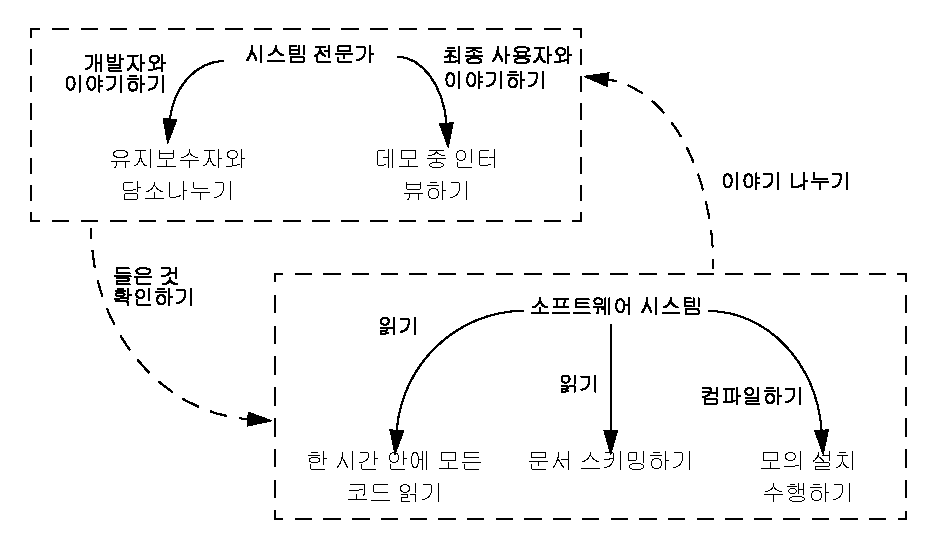
\includegraphics[width=\textwidth]{oldFirstContactMap.pdf}
\caption{시스템에 \charef{첫 번째 접근}{FirstContact}을 진행하는 동안 프로젝트의 \emph{구현가능성(feasbility)}을 평가한다.}
\figlabel{FirstContactMap}
\end{center}
\end{figure}

시스템과 처음 접촉할 때 시간 낭비가 가장 큰 리스크이므로 이러한 패턴은 1주일 정도의 짧은 기간 동안 적용해야 한다. 이번 주가 지나면 주요 이슈를 파악하고 그 지식을 바탕으로 추가 활동을 계획하거나 --- 필요한 경우 --- 프로젝트를 취소해야 한다.

\patref{유지보수자와 담소나누기}{ChatWithTheMaintainers} 및 \patref{데모 중 인터뷰하기}{InterviewDuringDemo} 패턴은 관련된 사람들과 친해지는 데 도움이 될 것이다. 경험상 4일 동안 정보를 수집하고 마지막 날을 사용하여 이 모든 정보를 첫 번째 프로젝트 계획으로 정리하자. 패턴을 적용하는 데 엄격한 순서는 없지만 책에서 제시하는 순서가 일종의 일반적인 순서이다. 그럼에도 불구하고 재차 확인해야 할 필요성 때문에 이러한 패턴의 조각을 조합하는 경우가 종종 있다. 예를 들어 유지보수자(maintainer)와의 두 번째 미팅에서는 보통 \patref{데모 중 인터뷰하기}{InterviewDuringDemo}로 시작하지만 \patref{한 시간 안에 모든 코드 읽기}{ReadAllTheCodeInOneHour}와 \patref{문서 스키밍하기}{SkimTheDocumentation}에서 배운 내용에 대해 질문을 하기도 한다. 또한 인터뷰가 끝나면 소스 코드와 문서를 빠르게 확인하여 말한 내용을 확인한다.

특정 상황에서는 리소스 부족으로 인해 일부 패턴이 적용되지 않는 경우가 있다. 예를 들어, 모든 유지보수자가 퇴사한 경우 \patref{유지보수자와 담소나누기}{ChatWithTheMaintainers}를 사용할 수 없다. 또한 특정 시스템에는 외부 사용자 인터페이스가 없기 때문에 최종 사용자와 \patref{데모 중 인터뷰하기}{InterviewDuringDemo}를 시도하는 것이 무의미할 수도 있다. 이러한 패턴 중 일부는 프로젝트 목표와 무관할 수 있으므로 반드시 문제가 되는 것은 아니다. 하지만 리소스의 부재는 프로젝트에 추가적인 리스크을 초래하므로 첫 번째 프로젝트 계획에 이를 기록해야 한다.

%-----------------------------------------------------------------
\subsection*{다음 단계}

필요한 정보를 확보했다면 이제 첫 번째 프로젝트 계획을 작성할 차례이다.이러한 계획은 프로젝트를 시작할 때 일반적으로 사용하는 계획과 매우 유사하므로 회사에서 사용하는 표준 문서 템플릿을 사용해야 한다. 필요한 경우 최소한 다음 항목이 포함되도록 규칙을 수정하자.

\begin{bulletlist}
  \item \emph{프로젝트 범위.}
프로젝트의 배경, 목표, 목표 달성 여부를 확인하는 데 사용할 기준을 포함하여 프로젝트에 대한 (반 페이지의) 간단한 설명을 준비한다. 계획의 이 부분을 작성하려면 \patpgref{사용자 참여시키기}{InvolveTheUsers} 및 \patpgref{맥심에 동의하기}{AgreeOnMaxims}를 사용한다.

  \item \emph{기회.}
프로젝트 목표를 달성하는 데 기여할 것으로 예상되는 요소를 파악하자. 숙련된 유자보수자와 파워 유저의 가용성(availability), 소스 코드의 가독성(readability) 또는 최신 문서의 존재 여부 등 첫 번째 접촉에서 발견한 항목을 나열하자.

  \item \emph{리스크.}
프로젝트 진행 중에 문제를 일으킬 수 있는 요소를 고려하자. 코드 라이브러리가 누락되었거나 테스트 슈트(test suite)가 없는 등 발견하지 못했거나 품질이 떨어지는 항목을 나열하자. 가능하면 각 리스크에 대한 발생가능성(likelihood)(가능성 없음, 가능성 보통, 가능성 높음)과 영향도(impact)(높음, 보통, 낮음)에 대한 평가를 포함하자. 특히 중요 리스크, 즉 발생가능성이 보통/높고 영향이 보통/높은 리스크 또는 가능성이 높고 영향이 낮은 위험에 대해 특별한 주의를 기울여야 합니다.

  \item \emph{진행/진행 불가 결정.}
어느 시점에서 프로젝트를 계속 진행할지 아니면 취소할지 결정해야 한다. 위의 기회와 리스크을 사용하여 그 결정에 대해 토론하자.

  \item \emph{활동.}
(``진행'' 결정의 경우) 프로젝트 목표를 어떻게 달성할 것인지 설명하면서 향후 기간에 대한 조망(fish-eye view)를 준비하자. 조망도에서는 단기 활동은 상당히 상세하게 설명하고, 이후 활동은 대략적인 개요로 충분하다. 대부분의 경우 단기 활동은 \charef{초기 이해}{InitialUnderstanding}에 설명된 패턴과 일치할 것이다. 이후 활동은 이후 챕터를 확인하자.

활동 목록은 기회를 활용하고 (중요한) 리스크 줄여야 한다. 예를 들어, 최신 문서가 있다는 것을 기회로, 테스트 슈트가 없다는 것을 중대한 리스크로 나열한 경우, 문서를 기반으로 테스트 스위트를 구축하는 활동을 계획해야 한다.

\end{bulletlist}

%=================================================================
%:PATTERN -- Chat with the Maintainers
\pattern{유지보수자와 담소나누기}{ChatWithTheMaintainers}

\intent{시스템 유지보수 담당자와의 토론을 통해 프로젝트의 역사적, 정치적 맥락에 대해 배워보자.}

\subsection*{문제}

리엔지니어링하려는 레거시 시스템의 역사적, 정치적 맥락을 제대로 파악하려면 어떻게 해야 하는가?

\emph{이 문제가 어려운 이유는 다음과 같다.}

\begin{bulletlist}
  \item 문서가 있는 경우 일반적으로 솔루션에 대한 결정은 기록하지만 솔루션에 영향을 준 요소에 대해서는 기록하지 않는다. 따라서 시스템의 역사에서 중요한 사건(즉, 역사적 맥락)은 거의 문서화되지 않는다.

  \item 시스템은 가치가 있지만(그렇지 않다면 시스템을 리엔지니어링할 필요가 없다) 경영진은 통제력을 상실했다(그렇지 않다면 시스템을 리엔지니어링할 필요가 없을 것이다). 소프트웨어 시스템과 관련된 사람 중 적어도 일부가 엉망이므로 레거시 시스템의 정치적 맥락은 본질적으로 문제가 있다.

  \item 시스템과 관련된 사람들이 사용자를 오도할 수 있다. 특히 시스템에서 문제가 있는 부분을 담당하거나 자신의 일자리를 보호하려는 경우 고의적으로 사용자를 속이는 경우가 있다. 대부분의 경우, 특히 수석 개발자가 다른 프로젝트에 참여하고 주니어 직원만 남아 시스템 유지보수를 담당할 때 무지에서 비롯된 오해를 불러일으킬 수 있다.

\end{bulletlist}

\emph{그러나 이 문제를 해결할 수 있는 이유는 다음과 같다.}

\begin{bulletlist}
  \item \emph{유지보수 팀(maintenance team)}과 논의할 수 있다. 그들은 원래 시스템 컨텍스트에 대해 모든 것을 알지 못할 수도 있지만 시스템이 현재 상태가 된 경위에 대해서는 상당 부분 알고 있을 가능성이 높다.
\end{bulletlist}

\subsection*{해결}

시스템 유자보수자와 논의하자. 레거시 시스템에 밀접하게 관여해 온 기술 담당자들은 시스템의 역사와 그 역사에 영향을 미친 사람 관련 문제를 잘 알고 있다.

오해의 소지가 있는 정보를 피하려면 유자보수자를 ``전우(brothers in arms)''로 대하자. 그들이 하는 일에 대해 설명하는 데 시간을 내준다면 그들의 일을 더 쉽게 해줄 수 있는 것(더 많은 보람, 더 많은 인정, --- 그들을 설득할 가능성이 가장 높은 것)을 제공하는 일종의 협상을 시도해 보자. 이렇게 하면 리엔지니어링 프로젝트의 후반 단계에서 필요한 존경심을 얻을 수 있다는 추가적인 이점도 있다.

\subsubsection*{힌트}

다음은 유자보수자와 논의할 때 도움이 될 수 있는 몇 가지 질문이다. 이러한 질문은 (공식 회의록이나 안건이 없는) 비공식 회의 중에 하는 것이 가장 좋지만, 회의가 끝난 후 주요 결론, 가정 및 우려 사항을 기록하기 위해 메모할 준비를 해야 한다.

\begin{bulletlist}
  \item 지난 한 달 동안 가장 쉽게 고칠 수 있었던 버그는 무엇이었나? 그리고 가장 어려웠던 버그는 무엇이었나? 각각을 고치는 데 얼마나 걸렸나? 특정 버그를 고치는 것이 왜 그렇게 쉬웠거나 어려웠나?

이러한 질문은 유지보수 작업에 관심이 있다는 것을 보여주기 때문에 좋은 출발점이 된다. 또한 이러한 질문에 답함으로써 유지보수자는 자신의 뛰어난 능력을 보여줄 수 있는 기회를 얻게 되어 업무에 대한 부담감을 덜 수 있다. 마지막으로, 답변은 나중에 더 높은 수준의 토론에서 사용할 수 있는 \ind{유지보수} 문제에 대한 몇 가지 구체적인 예를 제공한다.

  \item 유지보수 팀은 \ind{버그 리포트}\emph{(bug report)} 및 기능 요청을 어떻게 수집하는가? 어떤 요청을 먼저 처리할지는 누가 결정하는가? 버그 리포팅이나 기능 요청을 관리자에게 배정하는 것은 누가 결정하는가? 이러한 이벤트는 어떤 종류의 데이터베이스에 기록되는가? 버전 또는 구성 관리 시스템(configuration management system)\footnote{소프트웨어의 변경사항을 체계적으로 추적하고 통제하는 시스템으로 형상 관리 시스템이라고도 한다. git도 한 예이다. -옮긴이}이 마련되어 있는가?

이러한 질문은 유지보수 프로세스의 조직과 유지보수 팀의 내부 작업 습관을 이해하는 데 도움이 된다. 정치적 맥락에 관한 한 팀 내 관계(작업 할당)와 최종 사용자와의 관계(버그 리포트 수집)를 평가하는 데 도움이 된다.

  \item 오랫 동안 개발/유지보수 팀의 일원이었던 사람은 누구였는가? 프로젝트에 어떻게 합류/탈퇴했나? 이것이 시스템의 릴리스 기록에 어떤 영향을 미쳤나?

이러한 질문은 레거시 시스템의 역사를 직접적으로 다루는 질문이다. 사람들은 일반적으로 이전 동료에 대해 잘 기억하기 때문에 사람에 대해 물어보는 것이 좋다. 나중에 그들이 어떻게 프로젝트에 합류하거나 떠났는지 물어보면 정치적 맥락도 파악할 수 있다.

  \item 코드는 얼마나 좋은가? 문서는 얼마나 신뢰할 수 있는가?

이 질문은 특히 유지보수 팀 스스로가 시스템 상태를 얼마나 잘 평가할 수 있는지 확인하는 것과 관련이 있다. 물론 나중에 그들의 주장을 직접 확인해야 한다(\patref{한 시간 안에 모든 코드 읽기}{ReadAllTheCodeInOneHour} 및 \patref{문서 스키밍하기}{SkimTheDocumentation} 참조).

  \item 이 리엔지니어링 프로젝트를 시작한 이유는 무엇인가? 이 프로젝트에서 무엇을 기대하는가? 결과를 통해 무엇을 얻을 수 있는가?

리엔지니어링 프로젝트를 통해 유지보수자가 무엇을 얻을 수 있는지 묻는 것은 이후 단계에서 염두에 두어야 할 사항이므로 매우 중요히다. 경영진이 프로젝트에서 기대하는 것과 유지보수자가 기대하는 것의 (때로는 미묘한) 차이점에 귀를 기울이자. 차이점을 파악하면 정치적 맥락을 파악하는 데 도움이 된다.

\end{bulletlist}

\subsection*{트레이드오프}

\subsubsection*{장점}
\begin{bulletlist}
  \item \emph{정보를 효과적으로 얻는다.}
소프트웨어 시스템의 수명 주기에서 중요한 이벤트는 대부분 구두로 전달된다. 유지보수자와 토론하는 것이 이 풍부한 정보 소스를 활용하는 가장 효과적인 방법이다.

  \item \emph{동료와 친해지자.}
관리자와 토론하면 동료에 대해 처음으로 평가할 수 있는 기회를 갖게 됩니다. 따라서 리엔지니어링 프로젝트의 후반 단계에서 필요한 신뢰를 얻을 수 있을 것입니다.

\end{bulletlist}

\subsubsection*{단점}

\begin{bulletlist}
  \item \emph{사례 증거만 제공된다.}
여러분이 얻는 정보는 기껏해야 사례(anecdotal)일 뿐이다. 인간의 뇌는 어떤 사실을 기억하는지에 대해 선택적일 수밖에 없으므로 관리자의 기억이 불충분할 수 있다. 더 나쁜 것은 유지보수자가 시스템의 원래 개발자가 아닌 경우가 많기 때문에 정보가 처음부터 불완전할 수 있다는 것이다. 따라서 다른 방법으로 얻은 정보를 보완해야 한다(예: \patref{문서 스키밍하기}{SkimTheDocumentation}, \patref{데모 중 인터뷰하기}{InterviewDuringDemo}, \patref{한 시간 안에 모든 코드 읽기}{ReadAllTheCodeInOneHour} 및 \patref{모의 설치 하기}{DoAMockInstallation} 참조).

\end{bulletlist}

\subsubsection*{어려움}

\begin{bulletlist}
  \item \emph{사람들은 자신의 일자리를 보호한다.}
일부 유지보수자는 일자리를 잃을까 두려워서 필요한 정보를 제공하지 않을 수도 있다. 리엔지니어링 프로젝트가 그들의 업무를 더 쉽고, 더 보람 있고, 더 가치 있게 만들기 위해 존재한다는 것을 설득하는 것은 여러분의 몫이다. 따라서 유지보수자에게 리엔지니어링 프로젝트에서 무엇을 기대하는지 직접 물어봐야 한다.

  \item \emph{팀이 불안정할 수 있다.}
소프트웨어 유지보수는 일반적으로 2급 업무로 간주되어 주니어 프로그래머에게 맡기는 경우가 많으며 유지보수 팀이 자주 바뀌는 경우가 많다. 이러한 상황에서는 유자보수자가 소프트웨어 시스템의 역사적 진화에 대해 말할 수는 없지만, 그 정치적 맥락에 대해서는 많은 것을 알 수 있다. 실제로 팀의 불안정성은 프로젝트의 위험을 증가시키고 획득한 정보의 신뢰성을 떨어뜨리기 때문에 이러한 불안정성을 인지해야 한다. 따라서 수년 동안 개발/유지보수 팀의 일원이었던 사람이 누구인지 물어봐야 한다.

\end{bulletlist}

\subsection*{예시}

\emph{XDoctor}를 인수하는 동안 회사는 원래 개발 팀을 설득하여 두 소프트웨어 시스템을 하나로 통합하려고 노력해 왔다. 안타깝게도 팀원 중 한 명인 데이브만 남기로 동의하고 나머지 세 명은 다른 회사로 떠났다. 두 제품을 통합하는 방법에 대한 계획을 개발하는 것이 당신의 임무이므로 데이브를 점심 식사에 초대하여 시스템에 대한 비공식적인 대화를 나눈다.

이 대화를 통해 많은 것을 배우게 된다. 좋은 소식은 데이브가 건강 보험과의 거래를 처리하는 인터넷 통신 프로토콜을 구현하는 일을 담당했다는 것이다. 이 기능은 제품에 부족한 핵심 기능 중 하나였기 때문에 팀에 이러한 경험을 추가하게 되어 당신은 기쁠 것이다. 더 좋은 소식은 데이브의 전 동료가 객체 지향 기술에 대한 경험이 많았기 때문에 합리적인 설계와 가독성 높은 소스 코드를 기대할 수 있다는 것이다. 마지막으로 버그 리포트가 거의 제출되지 않았고 대부분의 버그가 빠르게 처리되었다는 이야기도 들었다. 마찬가지로 보류 중인 제품 개선 사항 목록이 존재하며 그 수가 상당히 적다. 따라서 고객들이 제품에 상당히 만족하고 있으며 이 프로젝트가 전략적으로 중요할 것이라고 결론을 내린다.

좋지 않은 소식은 데이브가 주로 동료들에게 무시당하고 나머지 시스템의 설계 활동에서 제외된 하드코어 C 프로그래머라는 것이다. 프로젝트에 남게 된 동기에 대해 물었을 때 그는 원래 인터넷 기술을 실험하는 데 관심이 있어서 합류했지만, 지금까지 해온 저수준 프로토콜 작업이 지루해져서 더 흥미로운 일을 하고 싶다고 말한다. 물론 '더 흥미로운 일'이 무슨 뜻인지 물어보니 그는 객체로 프로그래밍하고 싶다고 대답한다.

토론이 끝난 후 데이브가 작성한 코드의 품질을 평가하기 위해 소스 코드를 확인하기로 마음먹었다. 또한 보류 중인 버그 목록과 개선 요청을 살펴보고 병합해야 할 두 제품의 기능을 비교하고자 한다. 마지막으로 교육 부서에 연락하여 객체 지향 프로그래밍에 대한 강좌가 있는지 알아보는 것도 새 팀원에게 동기를 부여할 수 있는 방법이 될 수 있으므로 고려한다.

\subsection*{근거}

\index{디마르코, 톰}
\begin{quotation}
\noindent
\emph{``우리 업무의 주요 문제는 본질적으로 기술적인 것이 아니라 사회학적 문제이다.''}

\hfill --- 톰 디마르코, \cite{DeMa99a}
\end{quotation}

소프트웨어 프로젝트와 관련된 사회학적 문제가 기술적인 문제보다 훨씬 더 중요하다는 전제를 받아들인다면, 리엔지니어링 프로젝트 참여자들은 최소한 연구 대상 시스템의 정치적 맥락을 알아야 합니다.

\index{콘웨이, 멜빈}
\begin{quotation}
\noindent
\emph{``시스템을 설계하는 조직은 해당 조직의 커뮤니케이션 구조를 복사한 디자인을 만드는 제약을 가진다.''}

\hfill --- Melvin Conway, \cite{Conw68a}
\end{quotation}

\ind{콘웨이의 법칙}\emph{(Conway's law)}은 종종 다음과 같이 의역됩니다: ``컴파일러를 개발하는 그룹이 4개라면, 4패스 컴파일러(4-pass compiler)\footnote{4번의 분리된 단계를 거쳐야만 결과가 나오는 컴파일러-옮긴이}를 얻을 수 있다''

개발팀이 어떤 방식으로 구성되었는지 아는 것이 중요한 이유 중 하나는 이 구조가 소스 코드의 구조를 어느 정도 반영할 가능성이 높기 때문이다.

두 번째 이유는 리엔지니어링 프로젝트 계획을 수립하기 전에 팀원의 역량과 리버스 엔지니어링할 소프트웨어 시스템의 특성을 알아야 하기 때문이다. 유지보수자와의 토론은 이러한 지식을 얻는 방법 중 하나이며, ``시간은 부족하다(time is scarce)''는 원칙을 고려할 때 매우 효율적인 방법이다.

\index{톰셋, 롭}
\begin{quotation}
\noindent
\emph{``유지 보수 관련 사실 \#1. 60년대 후반과 70년대 내내 생산 시스템 지원 및 유지보수는 분명히 2급 업무(second-class work)로 취급되었다.\\.
유지보수 관련 사실 \#2. 1998년에도 생산 시스템 지원 및 유지보수는 계속해서 2급 업무로 취급되었다.''}

\hfill --- 롭 톰셋, \cite{Thom98a}
\end{quotation}

유지보수자와 이야기를 나누다 보면 소프트웨어 유지 관리가 2급 업무로 간주되는 경우가 많다는 사실을 알게 된다. 만약 여러분이 대화하는 유지보수 팀이 그런 경우라면 논의가 심각하게 방해받을 수 있다. 유지보수 팀이 자주 바뀌었기 때문일 수도 있고, 이 경우 유지보수자가 그간의 발전 과정을 잘 모르기 때문일 수도 있다. 또는 논의하는 사람들이 자신의 업무에 대해 매우 보호적인 태도를 취하기 때문에 여러분이 알아야 할 내용을 알려주지 않을 수도 있다. 

\subsection*{알려진 용도}

리엔지니어링 프로젝트를 진행하면서 유지보수 팀과의 회의를 하는 중에 프로젝트의 킥오프(kick-off)하는 습관을 만들었다. 돌이켜보면 이러한 회의가 나머지 프로젝트에 필요한 신뢰를 구축하는 데 얼마나 중요한지 알 수 있었다. 유자보수자는 자신의 직업에 대한 자부심이 강하고 비판에 매우 민감하다는 사실을 뼈저리게 깨달았다. 따라서 킥오프 미팅은 ``유자보수자 중심(maintainer oriented)''으로, 즉 유자보수자가 무엇을 잘하고 무엇을 더 잘하고 싶은지 보여줄 수 있도록 해야 한다는 점을 강조합니다. 초보인 내가 이 멍청한 관리자들에게 제대로 된 일을 하는 방법을 가르쳐주겠다는 태도로 참여하면 거의 틀림없이 재앙을 초래할 것입니다.

\index{루가버, 스펜서}
\index{화이트, 짐}
\begin{quotation}
\noindent
\emph{``\ind{RT-100} ---은 1980년대 후반 타사 소프트웨어 공급업체가 개발하여 1990년에 \ind{노텔(Nortel)}에 인수되었다. 이후 3년 동안 노텔은 이 시스템을 개선하고 유지보수한 후 다른 공급업체에 아웃소싱하여 체계적으로 재작성했다. 이 노력은 실패로 돌아갔고 시스템은 1994년 중반에 다시 노텔로 돌아왔다. 이 무렵에는 원래 설계 팀이 해체되어 흩어져 있었고 제품의 6개 고객 조직은 상당히 불만이 많았다.\\
RT-100은 노텔의 애틀랜타 테크놀로지 파크 연구소에 배정되었다. 그곳에는 ACD 소프트웨어에 대한 경험이 있는 직원이 없었고, 다른 프로젝트의 취소로 인해 직원들의 사기가 상당히 저하되어 있었다.''}

\hfill --- 스펜서 루가버, 짐 화이트, \cite{Ruga98a}
\end{quotation}

위의 인용문은 한 리엔지니어링 프로젝트의 사례를 설명하는 논문에서 인용한 것으로, 리엔지니어링 프로젝트가 시작될 때의 전형적인 절박함을 잘 묘사하고 있다. 하지만 --- 논문 자체에 설명되어 있듯이 --- 역사적, 정치적 맥락에 대한 이러한 초기 평가 덕분에 프로젝트가 성공할 수 있었던 것은 어떤 요소가 이해관계자들을 만족시키고 결과적으로 새로운 리엔지니어링 팀에게 동기를 부여할 수 있는지 잘 알고 있었기 때문이다.

\index{쿡, 스테펀}
\ind{DESEL 프로젝트}(시스템 진화의 용이성을 위한 설계)의 사례 연구 중 하나에서 스테펀 쿡은 도메인의 어떤 측면이 변경될 가능성이 있고 어떤 측면이 안정적으로 유지될 가능성이 있는지 가장 잘 알고 있는 유지보수자와 대화하는 것이 중요하다고 말한다 \cite{Cook01a}. 따라서 유자보수자는 시스템이 어떻게 구축될 수 있었는지에 대한 지식, 즉 거의 문서화되지 않은 지식을 가지고 있다. 그러나 이 논의 과정에서 ``진화를 위한 설계(design for evolution)''라는 사고방식을 강조하여 유자보수자가 자신이 해결해 온 최신의 여러 문제에서 벗어나도록 해야 한다.

\subsection*{관련 패턴}

소프트웨어 개발 팀의 조직 방식을 명시적으로 다루는 몇 가지 패턴 언어가 있다 \cite{Copl95d} \cite{Harri96a} \cite{Tayl00a} \cite{Beed00a}. 앞으로의 엔지니어링 상황을 위한 것이지만, 유지보수자와 논의할 때 상황을 더 빨리 평가하는 데 도움이 될 수 있으므로 이를 숙지하는 것이 좋다.

\subsection*{다음 단계}

토론하는 동안 섣불리 결론을 내리지 않도록 주의해야 한다. 따라서 토론을 통해 알게 된 내용은 다른 출처를 통해 확인해야 한다. 일반적으로 이러한 출처는 시스템을 사용하는 사람들(\patref{데모 중 인터뷰하기}{InterviewDuringDemo}), 문서(\patref{문서 스키밍하기}{SkimTheDocumentation}), 시스템 자체(예: \patref{한 시간 안에 모든 코드 읽기}{ReadAllTheCodeInOneHour}) 등이다. \patref{모의 설치 수행하기}{DoAMockInstallation}).

이 검증을 통해 프로젝트를 완전히 취소할 가능성을 포함하여 레거시 시스템 문제를 해결하기 위한 초기 계획을 세울 수 있는 확실한 근거를 마련할 수 있다. 유자보수자와의 논의는 다양한 방식으로 이 계획에 영향을 미친다. 우선, 유지보수 팀의 협력 의지를 파악할 수 있어 작업 계획에 상당한 영향을 미친다. 둘째, 시스템을 가치 있게 만드는 부분과 대부분의 유지보수 문제를 일으킨 이벤트를 포함하여 시스템의 역사를 알고 있다. 당신 회사의 계획은 가치 있는 부분을 되살리고 이러한 유지보수 문제를 해결하는 것을 목표로 할 것이다. 셋째, 유지보수 팀이 다른 이해관계자들과 어떻게 소통하는지에 대해 알게 되며, 이는 계획이 받아들여지는 데 중요하다.

%=================================================================
%:PATTERN -- Read all the Code in One Hour
\pattern{한 시간 안에 모든 코드 읽기}{ReadAllTheCodeInOneHour}

\intent{간단하지만 집중적인 코드 검토를 통해 소프트웨어 시스템의 상태를 평가한다.}

\subsection*{문제}

소스 코드의 품질에 대한 첫인상을 어떻게 얻을 수 있는가?

\emph{이 문제는 다음과 같은 이유로 어렵다.}

\begin{bulletlist}
  \item 소스 코드의 품질은 시스템의 개발 및 유지보수에 참여한 사람에 따라 상당히 달라질 수 있다.

  \item 시스템 규모가 커서 정확한 평가를 위해 검사해야 할 데이터가 너무 많다.

  \item 소프트웨어 시스템에 익숙하지 않아서 관련성이 있는 것을 필터링하는 방법을 모른다.
\end{bulletlist}

\emph{그러나 이 문제를 해결할 수 있는 이유는 다음과 같다.}

\begin{bulletlist}
  \item 여러분이 구현에 사용 중인 언어에 대한 합리적인 \emph{전문성(expertise)}이 있으므로 프로그래밍 관용구(programming idioms) 및 코드 스멜(code smells)을 인식할 수 있다.

  \item 여러분의 리엔지니어링 프로젝트에 명확한 목표가 있으므로 그 목표를 달성하는 데 필요한 코드 품질을 평가할 수 있습니다.

\end{bulletlist}

\subsection*{해결}

소스 코드를 읽을 수 있는 적당히 짧은 시간(예: 약 1시간)의 학습 시간을 스스로에게 부여하자. 방해받지 않도록 하고(전화기를 뽑고 이메일 연결을 끊고), 코드와 최대한 접촉할 수 있도록 메모를 아껴서 하자. 

이 읽기 세션이 끝나면 다음과 같은 내용을 포함한 간단한 보고서를 작성하자.
\begin{bulletlist}
  \item 리엔지니어링이 실현 가능한지 여부와 그 이유(혹은 안 되는 이유)에 대한 일반적인 평가 항목

  \item 중요해 보이는 엔티티(예: 클래스, 패키지, $\cdots$)

  \item 파악된 의심스러운 코딩 스타일(예: ``\ind{코드 스멜}'' \cite{Fowl99a});

  \item 추가 조사가 필요한 부분(예: 테스트).

\end{bulletlist}

이 보고서는 짧게 작성하고 소스 코드에 언급된 대로 엔티티의 이름을 언급한다.

\subsubsection*{힌트}

``시간은 부족하다(time is scarce)''는 원칙에 따라 약간의 준비가 필요하다. 체크리스트를 작성하면 읽기 세션에서 집중하는 데 도움이 될 수 있다. 이러한 체크리스트는 다양한 출처에서 가져와 작성할 수 있다.

\begin{bulletlist}
  \item 개발 팀에서 품질 보증의 일환으로 \emphind{코드 리뷰}\emph{(code review)}를 사용했을 수 있다. 사용했다면 리뷰에 사용된 체크리스트를 포함해야 한다. 그렇지 않다면 해당 코드의 종류를 검토하는 데 사용되는 일반적인 체크리스트를 사용해 보자.

  \item 일부 개발팀에서는 \emph{코딩 스타일(coding style)}을 적용하기도 하는데, 적용했다면 이를 알아두는 것이 좋다. 특히 명명 규칙(naming convention)은 코드를 빠르게 스캔하는 데 매우 중요하다.

  \item 프로그래머는 \emphind{코딩 이디엄}\emph{(coding idiom)}(예: C++ \cite{Copl92a} \cite{Meye98a} \cite{Meye96a}; Smalltalk \cite{Beck97a})를 사용하여 일반적인 언어 구성을 인식할 수 있다.

  \item 답변을 듣고 싶은 \emph{질문(question)}이 있을 수 있다.
\end{bulletlist}

다음은 추가 검토를 위한 좋은 시작점을 제공하기 때문에 체크리스트에 추가할 수 있는 몇 가지 항목이다.

\begin{bulletlist}
  \item \emph{기능 테스트(functonal test) 및 \ind{단위 테스트}(unit test)}는 소프트웨어 시스템의 기능에 대한 중요한 정보를 전달한다. 이러한 테스트는 시스템이 예상대로 작동하는지 확인하는 데 도움이 되며, 이는 리엔지니어링 중에 매우 중요하다(\charef{테스트라는 생명 보험}{TestsYourLifeInsurance} 참조).

  \item \emph{추상 클래스 및 메서드}는 설계 의도를 드러낸다.

  \item 계층 구조에서 상위 클래스는 종종 도메인 추상화를 정의하고, 하위 클래스는 이에 대한 변형을 도입하도록 돕는다.

  \item \patpgref{싱글톤}{Singleton} 패턴의 발생은 시스템의 전체 실행에 대해 일정한 정보를 나타낼 수 있다.

  \item 놀랍게도 \emph{대형 구조체}는 종종 중요한 기능 덩어리를 지정한다.

  \item \emph{주석(comment)}은 특정 코드의 설계 의도에 대해 많은 것을 알려주지만, 종종 오해의 소지가 있을 수 있다.

\end{bulletlist}


\subsection*{트레이드오프}

\subsubsection*{장점}
\begin{bulletlist}
  \item \emph{효율적으로 시작하자.}
짧은 시간 안에 코드를 읽는 것은 초보자로서 매우 효율적이다. 실제로 시간을 제한하면서도 모든 코드를 살펴보도록 강요하면 두뇌와 코딩 전문 지식을 주로 사용하여 중요해 보이는 부분을 걸러낼 수 있다.

  \item \emph{성실하게 판단하자.}
코드를 직접 읽으면 소프트웨어 시스템에 대한 편견 없는 시각을 갖게 되고, 세부 사항에 대한 감각과 직면하고 있는 문제의 종류를 엿볼 수 있다. 소스 코드는 시스템의 기능을 설명하기 때문에 그 이상도 이하도 아닌 유일한 정확한 정보의 원천이다.

  \item \emph{개발자 어휘를 익히자.}
소프트웨어 시스템 내부에서 사용되는 어휘를 습득하는 것은 시스템을 이해하고 다른 개발자와 소통하는 데 필수적이다. 이 패턴은 이러한 어휘를 습득하는 데 도움이 된다.

\end{bulletlist}

\subsubsection*{단점}
\begin{bulletlist}
  \item \emph{낮은 수준의 추상화만 획득가능하다.}
이 패턴을 통해 솔루션 도메인에 대한 인사이트를 어느 정도 얻을 수 있지만, 이것이 문제 도메인 개념에 어떻게 매핑되는지에 대해서는 거의 알 수 없다. 따라서 더 추상적인 다른 표현으로 얻은 정보를 보완해야 한다(예: \patref{문서 스키밍하기}{SkimTheDocumentation} 및 \patref{데모 중 인터뷰하기}{InterviewDuringDemo}).
\end{bulletlist}

\subsubsection*{어려움}

\begin{bulletlist}
  \item \emph{큰 규모를 다루기 어렵다.}
\emph{모두}를 읽는 방법은 크기가 큰 코드를 다루기 어렵게 하며, 경험상 시간당 10,000줄의 코드가 적당하다. 크고 복잡한 코드를 마주할 때는 짧은 시간(2시간 이내)에 집중적으로 읽는 것이 가장 효과적이므로 더 많은 시간을 할애하여 코드를 읽으려고 하지 않는다. 대신 소스 코드를 분할할 명확한 기준이 있다면 일련의 세션을 나눠서 진행하자. 그렇지 않다면 모든 코드를 살펴보고 다른 부분보다 더 중요해 보이는 부분을 표시한 다음 \patref {유지보수자와 담소나누기}{ChatWithTheMaintainers}에 따라 다른 세션에서 읽으면 된다.

그러나 ``시간은 부족하다(Time is Scarce)''는 원칙을 고려할 때 간결하게 작성해야 한다. 따라서 크고 복잡한 코드를 다룰 때는 세부 사항에 너무 신경 쓰지 말고 리엔지니어링 적합성에 대한 초기 평가라는 코드 읽기의 목표를 상기하자.

  \item \emph{주석이 오해를 불러일으킬 수 있다.}
코드의 주석에 주의를 기울이자. 코멘트는 소프트웨어의 기능을 이해하는 데 도움이 될 수 있다. 하지만 다른 종류의 문서와 마찬가지로 주석도 오래되었거나 더 이상 사용되지 않거나 단순히 잘못된 것일 수 있다. 따라서 주석을 찾을 때는 체크리스트에 해당 주석이 도움이 되는지, 오래되었는지 여부를 표시하자.
\end{bulletlist}

\subsection*{예시}

데이브(원래 개발팀에서 유일하게 남은 사람으로 저수준 C 코드를 담당했던 사람)와의 토론에서, 여러분은 그들의 시스템이 주로 Java로 작성되었고 일부 저수준 부분은 C로, 데이터베이스 쿼리는 SQL로 작성되었다는 것을 기억할 것이다. 이 모든 언어에 대한 경험이 있으므로 코드를 읽을 수 있다.

먼저 체크리스트를 작성하고 일반적인 항목(코딩 스타일, 테스트, 추상 클래스 및 메서드, 계층 구조에서 상위 클래스, $\cdots$) 외에 해결하고 싶은 몇 가지 질문에 관한 몇 가지 항목을 추가한다. 그 중 하나는 ``C 코드의 가독성(readability of the C-code)''인데, 새 팀원인 데이브의 코딩 스타일을 확인하고 싶기 때문이다. 두 번째는 ``데이터베이스 스키마의 품질(quality of the database schema)''인데, 조만간 두 시스템의 데이터를 통합해야 한다는 것을 알고 있기 때문이다. 세 번째는 ``통화 처리(handling of currencies)''이다. 스위스가 유로 지역에 가입하고 6개월 이내에 모든 금융 데이터를 이 새로운 통화로 변환해야 하기 때문이다.

C 코드를 읽다 보면 이 부분이 상당히 난해하다는 것을 알 수 있다(수수께끼 같은 약어로 된 짧은 식별자, 긴 다중 출구 루프, $\cdots$). 그럼에도 불구하고 인터넷 프로토콜을 처리하는 모듈에는 단위 테스트가 있으므로 시스템에 통합할 가능성에 대해 더 확신을 가질 수 있다.

Java 코드는 한 시간에 50.000줄의 코드를 읽을 수 없다는 규모의 문제가 있다. 따라서 무작위로 몇 개의 파일을 선택하면 대부분의 클래스 이름에 \ct{UI} 또는 \ct{DB}라는 두 글자 접두사가 붙는 것을 발견할 수 있다. 2 계층 아키텍처(2-tiered architecture)(데이터베이스 계층과 사용자 인터페이스 계층)를 나타내는 명명 규칙을 의심하고 이를 자세히 조사하기 위해 메모를 작성한다. 또한 다양한 클래스 및 속성 이름이 의료 도메인에 의미 있는 것으로 인식한다(예: 이름, 주소, 건강 보험, $\cdots$ 속성을 가진 클래스 \ct{DBPatient}). 심지어 \ct{DBCurrency} 클래스를 인식하므로 개발자가 필요한 예방 조치를 취했기 때문에 유로로 전환해도 큰 문제가 발생하지 않을 것이라고 가정한다. 대부분의 클래스와 메서드에는 \ind{Javadoc} 규칙을 따르는 주석이 있으므로 적어도 일부 문서는 최신 상태일 것으로 예상한다. 마지막으로, 화면에 표시되는 다양한 문자열을 포함하는 대형 싱글톤 객체를 식별하여 시스템을 지역화할 수 있을 것이라는 결론을 내린다.

이 모든 것이 다소 희망적으로 보이지만 실망스러운 부분도 많이 있다. 가장 비관적인 이유는 매개변수 목록이 많고 조건문이 복잡한 긴 메서드가 많다는 점이다. 이들 중 상당수는 UI 로직(버튼과 메뉴 항목의 활성화/비활성화)과 비즈니스 로직(데이터베이스 레코드 업데이트)이 혼합되어 있는 것 같다. 한 가지(가격 계산)가 특히 복잡해 보이므로 이를 더 조사하기 위해 메모를 작성한다.

데이터베이스와 관련해서는 의료 서비스 도메인의 맥락에서 의미 있는 다양한 테이블 이름과 열 이름을 다시 인식한다. 언뜻 보기에는 스키마가 정규화된 것처럼 보이므로 여기에서도 리버스 엔지니어링이 횩허거 있을 것으로 보인다. 이 데이터베이스는 또한 일부 저장 프로시저를 사용하므로 추가 조사가 필요하다.

읽기 세션이 끝나면 다음 노트에 결론을 요약한다.

\begin{bulletlist}
  \item 인터넷 프로토콜 통합이 가능함: 단위 테스트와 담당 프로그래머가 있다.

  \item 명명 규칙에 따라 2계층 아키텍처가 의심됨: 비즈니스 로직은 어떤가? --- UI와 혼합되어 있는가? (추가 확인 필요!)

  \item 의미 있는 식별자가 포함되어 있는 읽을 수 있는 코드: 리버스 엔지니어링의 효과가 기대된다.

  \item 통화 개체 존재: 유로 변환이 가능해 보인다(추가 조사!).

  \item 사용된 자바독(Javadoc) 규칙 사용: 문서 확인이 필요하다.

  \item 가격 계산이 복잡해 보임: 그 이유는 무엇인가?

  \item 데이터베이스 스키마가 유용해 보임: 저장 절차는 추가 조사가 필요합니다.

\end{bulletlist}

\subsection*{근거}

코드 리뷰(coder review)는 동료가 작성한 프로그램에서 문제를 찾는 데 매우 효과적인 수단으로 널리 인정받고 있다 \cite{Gilb93a} \cite{Glass97a}. 이러한 검토를 비용 효율적으로 수행하기 위해서는 두 가지 중요한 전제 조건이 충족되어야 합니다: (a) 검토자가 관련 질문에 집중할 수 있도록 \emph{체크리스트(checklist)}를 준비해야 하고, (b) 리뷰어는 장시간(최대 2시간) 집중할 수 없으므로 리뷰 세션은 \emph{짧게} 유지해야 한다.

\index{코니그스버그, 앨런}
\begin{quotation}
\noindent
\emph{나는 속독 강좌를 들었고 '전쟁과 평화'를 20분 만에 읽었다. 러시아에 관한 책이다.}

\hfill --- 우디 앨런
\end{quotation}

기존의 코드 리뷰와 소프트웨어 시스템을 처음 접할 때 수행하는 코드 리뷰에는 중요한 차이점이 있다. 전자는 일반적으로 오류를 감지하기 위한 것이고, 후자는 첫인상을 얻기 위한 것이다. 이 차이는 세부 사항에 덜 신경을 써야 하므로 더 많은 코드를 읽을 수 있다는 것을 의미한다. 코드 리뷰에 대한 일반적인 가이드라인에서는 시간당 약 150개의 문을 검토할 수 있다고 명시하고 있다 \cite{Barn94a}. 그러나 첫 번째 접촉에서는 이러한 상세한 분석이 필요하지 않으므로 검토할 코드의 양을 늘릴 수 있다. 심각한 경험적 조사를 수행하지는 않았지만 경험상 시간당 10,000줄의 코드가 적당해 보인다.

\subsection*{알려진 용도}

\index{벡, 켄트}
이 패턴은 켄트 벡이 제안한 것으로, 그는 기존 시스템에서 컨설턴트 업무를 시작할 때 항상 적용하는 기법 중 하나라고 말했다. 롭슨은 코드 읽기를 ``시스템에 대한 지식을 얻는 가장 조잡한 방법(crudest method)''으로 보고하며, 기존 프로그램을 이해하는 데 가장 일반적으로 사용되는 방법이라고 인정한다{Robs91a}. 일부 사례 연구 보고서에서도 소스 코드 읽기가 리엔지니어링 프로젝트를 시작하는 방법 중 하나라고 언급하고 있다 \cite{Bray95a} \cite{Jack00a}.

이 패턴을 작성하는 동안 우리 팀원 중 한 명이 이 패턴을 적용하여 \ind{리팩토링 브라우저}(Refactoring Browser)를 리버스 엔지니어링했다. \cite{Robe97a}. 그 사람은 \ind{Smalltalk}에 익숙하지 않았지만 클래스 인터페이스를 검사하는 것만으로도 시스템 구조에 대한 느낌을 얻을 수 있었다. 또한 특수 계층 구조 브라우저는 주요 클래스 중 일부를 식별하는 데 도움이 되었고 주석은 코드의 어떤 부분을 수행해야 하는지에 대한 유용한 힌트를 제공했다. 패턴을 적용하는 데는 1시간이 조금 넘게 걸렸는데, 비교적 작은 시스템과 Smalltalk에 익숙하지 않아서 진행 속도가 느려 보였기 때문에 이 정도면 충분해 보였다.

이 패턴의 특히 흥미로운 사례는 \ind{FAMOOS} 프로젝트가 끝날 무렵에 발생했다. 일주일 동안 이질적인 리버스 엔지니어들로 구성된 팀이 일종의 리버스 엔지니어링 경연 대회에 참가하기 위해 현장 방문을 떠났다. 4일 동안 주어진 리버스 엔지니어링 도구를 사용하여 특정 \ind{C++} 시스템에 대해 최대한 많은 것을 배우는 것이 과제였다. 그런 다음 5일째에는 원래 개발자에게 결과를 보고하여 검증을 받는 것이었다. 팀원 중 한 명이 과제를 너무 일찍 끝내고 \patref{한 시간 안에 모든 코드 읽기}{ReadAllTheCodeInOneHour}에 도전하는 기회를 가졌다. 이 한 사람은 모든 토론에 참여할 수 있고 개발자의 의견 중 일부를 설명할 수 있을 정도로 시스템에 대해 훨씬 더 잘 파악하고 있었습니다.

\subsection*{다음 단계}

\patref{한 시간 안에 모든 코드 읽기}{ReadAllTheCodeInOneHour}를 완료한 후에는 리엔지니어링에 적합한지 평가하기 위해 \patref{모의 설치 수행하기}{DoAMockInstallation}을 수행해야 한다. 또한 \patref{문서 스키밍하기}{SkimTheDocumentation}를 수행하여 결과를 보완하고, 시스템을 일관성 있게 파악할 수 있는 기회를 극대화하기 위해 \patref{데모 중 인터뷰하기}{InterviewDuringDemo}를 수행하면 된다. 실제로 리엔지니어링 프로젝트를 어떻게 진행할지 결정하기 전에 \patref{유지보수자와 담소나누기}{ChatWithTheMaintainers}를 한 번 더 수행하는 것이 좋다.

시스템과의 첫 접촉이 끝나면 프로젝트를 어떻게 진행할지(또는 취소할지) 결정해야 한다. 코드를 읽으면 다양한 방식으로 이 결정에 영향을 미친다. 우선, 코드의 품질(예: 코딩 이디엄 및 의심스러운 코딩 스타일의 존재 여부)을 평가하여 프로젝트 리엔지니어링의 타당성을 평가했다. 둘째, 추가 탐색을 위한 좋은 출발점이 될 수 있는 몇 가지 중요한 엔티티를 식별했다. 

중요한 엔티티(예: 클래스, 패키지, \patref{한 시간 안에 모든 코드 읽기}{ReadAllTheCodeInOneHour}의 결과인 클래스, 패키지, $\cdots$) 목록을 사용하여 \patpgref{퍼시스턴트 데이터 분석하기}{AnalyzeThePersistentData} 및 \patpgref{예외적인 엔티티 연구하기}{StudyTheExceptionalEntities}를 시작할 수 있다. 이렇게 하면 소스 코드, 특히 문제 도메인을 나타내는 방식에 대해 구체적으로 이해할 수 있다.

%=================================================================
%:PATTERN -- Skim the Documentation
\pattern{문서 스키밍하기}{SkimTheDocumentation}

\intent{제한된 시간 내에 \ind{문서}(documentation)를 읽고 관련성을 평가한다.}

\subsection*{문제}

문서에서 도움이 될 수 있는 부분을 어떻게 식별할 수 있는가?

\emph{이 문제는 다음과 같은 이유로 어렵다.}

\begin{bulletlist}
  \item 문서가 있는 경우 개발팀이나 최종 사용자를 위한 것이므로 일반적으로 리엔지니어링 목적과 즉각적인 관련이 없다. 더 좋지 않은 것은 일반적으로 현재 상황과 관련하여 최신 정보가 아니므로 오해의 소지가 있는 정보가 포함되어 있을 수 있다는 것이다.

  \item 리엔지니어링 프로젝트가 어떻게 진행될지 아직 알 수 없으므로 문서의 어느 부분이 관련성이 있는지 알 수 없다.
\end{bulletlist}


\emph{그러나 이 문제를 해결할 수 있는 이유는 다음과 같다.}

\begin{bulletlist}
  \item 어떤 형태의 \emph{문서(documentation)}를 사용할 수 있으므로 적어도 시스템과 관련된 사람을 돕기 위한 설명이 있다.

  \item 여러분의 리엔지니어링 프로젝트에는 \emph{명확한 목표(clear goal)}가 있으므로 문서에서 가치 있는 부분과 쓸모없는 부분을 선택할 수 있다.

\end{bulletlist}

\subsection*{해결}

리엔지니어링 프로젝트에 흥미로워 보이는 시스템 측면을 요약한 목록을 준비하자. 그런 다음, 이 목록을 문서와 대조하면서 문서가 얼마나 최신 상태인지 대략적으로 평가하자. 마지막으로 다음과 같이 간단한 보고서로 결과를 요약하자.

\begin{bulletlist}
  \item 시스템 문서가 유용한지 여부와 그 이유 (혹은 그렇지 않은 이유)에 대한 일반적인 평가를 적는다.

  \item 문서에서 유용하다고 생각되는 부분의 목록과 그 이유(예: 요구 사항 사양, 원하는 기능, 중요한 제약 조건, 설계 다이어그램, 사용자 및 운영자 설명서)를 작성한다.

  \item 각 부분에 대해 설명이 얼마나 최신 상태인지에 대한 인상을 작성한다.
\end{bulletlist}

\subsubsection*{힌트}

리엔지니어링 프로젝트의 목표와 사용 중인 문서의 종류에 따라 주요 관심사에 맞게 읽기 프로세스를 조정할 수 있다. 예를 들어 원래 시스템 요구 사항에 대한 인사이트를 얻고 싶다면 시스템 사양을 살펴보고, 실제로 구현된 기능에 대한 지식은 최종 사용자 설명서나 튜토리얼 노트에서 수집해야 한다. 여유가 있다면 설계 문서(예: 클래스 다이어그램, 데이터베이스 스키마, $\cdots$)를 이해하려고 너무 많은 시간을 소비하지 말고, 리엔지니어링의 후반 단계에서 큰 도움이 될 수 있으므로 이러한 문서의 존재 여부와 신뢰성을 기록해 두자. 

실제 시스템과 관련하여 문서가 오래되지는 않았는지 확인하자. 항상 시스템 납품 날짜와 버전 날짜를 비교하고 신뢰할 수 없는 것으로 의심되는 부분을 기록해 두자. 

시간이 제한되어 있다는 사실 때문에 가장 유용한 정보를 추출할 수 있는 방법을 생각해야 한다. 다음은 주의해야 할 사항에 대한 몇 가지 힌트이다.

\begin{bulletlist}
  \item \emph{목차(table of contents)}는 구조와 제시된 정보에 대한 간략한 개요를 제공한다.

  \item \emph{버전 정보 및 날짜(Version numbers and dates)}는 문서의 해당 부분이 얼마나 최신 상태인지 알려준다.

  \item \emph{그림(figure)}은 정보를 전달하기 위한 좋은 수단이다. 그림 목록이 있는 경우 문서의 특정 부분에 대한 빠른 액세스 경로를 제공할 수 있다.

  \item \emph{화면 덤프(screen-dump), 샘플 출력물(print-out), 샘플 리포트(report), 명령어 설명(command description)}은 시스템에서 제공하는 기능에 대해 많은 것을 알려준다.

  \item \emph{정식 사양(formal specifications)}(예: 상태 차트(state-chart))이 있는 경우 일반적으로 중요한 기능에 해당한다.

  \item \emph{색인(index)}가 있는 경우에는 작성자가 중요하다고 생각하는 용어가 포함되어 있습니다.
\end{bulletlist}

\subsection*{트레이드오프}

\subsubsection*{장점}

\begin{bulletlist}
  \item \emph{높은 추상화 수준을 제공한다.}
문서는 사람이 읽어야 하므로 일정 수준의 추상화가 필요하다. 이 추상화 수준이 리엔지니어링 프로젝트에 충분히 높지 않을 수도 있지만 적어도 몇 가지 디코딩 단계를 건너뛸 수 있다.

  \item \emph{관련 부분에 집중한.}
흥미로워 보이는 부분의 목록을 미리 준비하면 읽기 세션이 목표 지향적이 되어 가치 있는 것을 찾을 확률이 높아진다. 또한 설명이 얼마나 최신인지 빠르게 평가할 수 있어 관련 없는 부분에 시간을 낭비하지 않아도 된다.
\end{bulletlist}

\subsubsection*{단점}

\begin{bulletlist}
  \item \emph{중요한 사실 누락한다.}
개요 모드에서 빠르게 읽으면 문서에 기록된 중요한 사실을 놓칠 수 있다. 하지만 찾고자 하는 내용을 목록으로 작성하면 이러한 효과를 어느 정도 줄일 수 있다.

  \item \emph{관련 없는 정보만 찾을 수 있다.}
문서의 어느 부분도 리엔지니어링 프로젝트와 관련이 없는 것처럼 보일 가능성이 적다. 그런 상황에서도 이제 문서에 대해 걱정하지 않아도 되니 읽는 데 들인 시간은 가치가 있다.

\end{bulletlist}

\subsubsection*{어려움}

\begin{bulletlist}
  \item \emph{다른 청중을 대상으로 한다.}
문서는 제작 비용이 많이 들기 때문에 최종 사용자(예: 사용자 매뉴얼) 또는 개발팀(예: 디자인)을 위해 작성된다. 또한 문서를 유지 관리하는 데도 많은 비용이 들기 때문에 시스템의 안정적인 부분만 문서화한다. 따라서 찾은 정보는 직접적인 관련이 없을 수 있으므로 신중한 해석이 필요하다.

  \item \emph{문서에 불일치가 있다.}
문서는 실제 상황과 관련하여 거의 항상 최신 정보가 아니다. 리엔지니어링 프로젝트의 초기 단계에서는 이러한 불일치를 인식할 수 있는 지식이 부족하기 때문에 이는 매우 위험하다. 따라서 문서에만 의존하여 중요한 결정을 내리지 말고, 먼저 다른 방법으로 결과를 확인하기 바란다, \patref{한 시간 안에 모든 코드 읽기}{ReadAllTheCodeInOneHour} 및 \patref{데모 중 인터뷰하기}{InterviewDuringDemo}).
\end{bulletlist}

\subsection*{예시}

데이브와의 비공식적인 대화와 코드 읽기 세션이 끝나면 시스템의 흥미로운 측면이 무엇인지 대략적으로 파악할 수 있다. 관련 정보가 포함되어 있는지 확인하기 위해 문서를 훑어보기로 결정한다.

읽고 싶은 측면의 목록을 작성하여 스스로 준비한다. 디자인 다이어그램, 클래스 인터페이스 설명(자바독?), 데이터베이스 스키마와 같은 당연한 항목 외에도 유로(사용자 설명서에 유로 변환에 대한 내용이 있는가?), 인터넷 프로토콜 사양 등이 목록에 포함되어 있다.

다음으로 데이브에게 가서 소프트웨어 시스템과 관련된 모든 문서를 요청한다. 데이브는 작은 미소를 지으며 여러분을 바라본다. ``정말 다 읽어보실 건 아니죠?'' ``꼭 그렇지는 않아요.'' ``하지만 적어도 이걸로 뭔가 할 수 있는지는 알고 싶어요.''라고 말한다. 데이브가 아까 준 상자를 살펴보고 종이로 가득 찬 폴더 3개 --- 설계 문서 ---와 소책자 1개 --- 사용 설명서를 건네준다.

사용 설명서부터 시작해서 --- 빙고: 색인에서 유로에 대한 항목을 발견한다. 해당 페이지를 넘기면 유로가 실제로 약 5페이지로 구성된 하나의 챕터라는 것을 알 수 있으므로 해당 페이지 번호를 표시하여 추가 학습을 진행한다. 다음으로 목차를 훑어보면 '프랑스어/독일어로 전환하기'라는 제목이 있다. 이 페이지를 읽으면 소프트웨어 현지화가 문서화된 기능이라는 것을 알 수 있다. 현지화는 체크리스트에 없었지만 여전히 중요하므로 기꺼이 이에 대한 메모를 추가한다. 이 모든 것이 상당히 유망해 보이므로 사용자 설명서의 릴리스 날짜를 확인하면 꽤 최근의 것임을 알 수 있다. 정말 좋은 시작이다!

디자인 문서의 첫 번째 폴더('클래스라는 제목의 폴더)를 열면 예상했던 것과 거의 비슷하게 Javadoc에서 생성된 클래스 인터페이스의 인쇄물을 찾을 수 있다. 종이로 읽는 것은 그다지 흥미롭지 않지만 어쨌든 페이지를 계속 훑어보게 된다. 첫인상은 각 클래스와 메서드와 함께 제공되는 실제 설명이 상당히 얕다는 것이다. 무작위로 세 페이지를 더 자세히 살펴보면 이러한 인상은 더욱 확고해진다. 다음으로 인터넷 프로토콜을 구현하는 C 코드와 인터페이스하는 클래스에 대한 설명을 찾아보면 빈 설명도 발견할 수 있다. 문서의 릴리스 날짜를 리트머스 테스트한 결과 이 문서가 상당히 오래되었다는 것을 알았으므로 온라인 문서를 확인하기 위해 메모를 작성한다.

두 번째 폴더에는 데이터베이스 스키마에 대한 생성된 설명이 들어 있는데, 각 테이블에 대해 각 열의 목적이 무엇인지 설명한다. 자바독 클래스 인터페이스 설명과 마찬가지로 문서 자체는 내용이 적어도 데이터베이스의 각 레코드가 무엇을 나타내야 하는지를 찾을 수 있는 방법이 있다. 여기에서도 문서 릴리스 날짜가 확인하니 동일한 문서의 온라인 버전을 확인하는 것이 필요하다는 것도 알 수 있다.

언뜻 보기에 세 번째 폴더에는 프로젝트와 막연하게 관련만 있어 보이는 다양한 잡다한 문서 사본이 들어 있는 것처럼 보인다. 첫 번째 문서는 의약품 가격 목록이고, 다음 열 개는 의료법에서 발췌한 것이다. 하지만 계속해서 페이지를 넘기다 보면 건강보험과 통신하는 데 사용되는 인터넷 프로토콜을 설명하는 것으로 보이는 유한 상태 다이어그램(finite state diagram)을 발견하게 된다. 분명히 이 문서는 기술 사양의 일부 페이지를 복사한 것이지만 안타깝게도 원본에 대한 참조는 포함되어 있지 않다. 이 문서의 릴리스 날짜도 누락되어 있어 이 사양이 오래된 것인지 확인할 수 있는 방법이 없다.

다음 보고서를 작성하고 읽기 세션을 마무리한다.

\begin{bulletlist}
  \item 사용자 설명서가 명확하고 최신 상태임: 기능에 대한 블랙박스 타입의 설명을 위한 좋은 참고처이다.

  \item 유로 화폐 관련 정보가 제공됨(513-518쪽): 현지화도 제공된다(723-725쪽).

  \item 클래스 인터페이스 설명이 생성되어 있음: 정보가 적지만 온라인에서 확인 가능하다.

  \item 데이터베이스 스키마에 대한 문서가 생성됨: 간략하지만 온라인에서 확인 가능하다.

  \item 인터넷 프로토콜에 대한 유한 상태 머신: 상태 의심스럽다. 데이브에게 에게 확인하도록 한다.

  \item 기타 문서(가격표, 지침 전단지, $\cdots$)가 들어 있는 폴더 1개
\end{bulletlist}

\subsection*{근거}

\index{프레스맨, 로저}
\begin{quotation}
\noindent
\emph{``소프트웨어 개발 조직에서 전체 소프트웨어 개발 노력의 20\~30\%를 문서화에 사용하는 것은 드문 일이 아니다.''}

\hfill --- 로저 프레스맨, \cite{Pres94a} 
\end{quotation}

소스코드와 달리 문서는 소프트웨어 시스템을 인간에게 적합한 추상화 수준에서 설명하기 위한 것이다. 따라서 문서에는 분명히 정보 ``덩어리(nugget)''가 포함될 것이며, 문제는 관련 정보를 찾는 방법이다. 거의 모든 리엔지니어링 프로젝트에 존재하는 두 가지 일반적인 상황 때문에 관련 정보를 찾는 것이 어렵다.

\begin{quotation}
\noindent
\emph{``모든 사례 연구에서 문서가 존재하지 않거나 불만족스럽거나 일관성이 없다는 문제에 직면한다.-''}

\noindent
--- ESEC/FSE 1997 Workshop on Object-Oriented \\
Re-engineering, \cite{Deme97a}
\end{quotation}

우선, 문서가 실제 상황과 일치하지 않을 가능성이 높다. ind{FAMOOS} 프로젝트에서 조사한 5개의 사례 연구에서 모든 관리자가 불만을 제기한 유일한 문제는 '불충분한 문서화'였다. 그럼에도 불구하고 오래된 정보라도 적어도 과거에 시스템이 어떻게 작동해야 했는지 알려주기 때문에 유용할 수 있다. 오늘날 어떻게 사용되는지 유추할 수 있는 좋은 출발점이다.

\index{웡, 케니}
\begin{quotation}
\noindent
\emph{``이러한 시스템에 대해 존재하는 문서는 일반적으로 전체 아키텍처가 아닌 개별적인 부분에 대해 설명한다. 게다가 문서는 시스템 전체와 여러 미디어에 흩어져 있는 경우가 많다.''}

\hfill 케니 웡, \etal, \cite{Wong95a}
\end{quotation}

둘째, 문서는 일반적으로 포워드 엔지니어링 컨텍스트에서 생성되므로 리엔지니어링 목적이 아니다. 예를 들어, 생성된 설계 문서(예: 데이터베이스 스키마, 자바독)는 일반적으로 상당히 최신이지만 너무 세분화되어 있어 리엔지니어링 프로젝트의 초기 단계에서는 유용하지 않다. 사용 설명서는 소프트웨어 시스템에 대한 블랙박스 타입의 설명이므로 그 안에 무엇이 들어 있는지에 대한 청사진 역할을 할 수 없다. 여기에서도 설명서를 실제로 관심 있는 부분을 유추할 수 있는 좋은 출발점으로 삼아야 한다.

\subsection*{알려진 용도}

피엘드슈타트와 햄렌의 연구에 따르면 '유지보수 프로그래머는 기능을 개선할 때 문서를 공부하는 시간보다 원래 프로그램을 공부하는 시간이 약 3.5배 더 길지만, 개선 기능을 구현하는 데 소요되는 시간은 그만큼 더 길다'고 합니다. \cite{Corb89a}, \cite{Fjel79a}. 이 등식은 문서 연구의 상대적 중요성에 대한 설명으로 받아 들일 수 있다.

\index{잭슨, 다니엘}
\index{채핀, 존}
\begin{quotation}
\noindent
\emph{``사례 연구는 CTAS의 기존 설계 전반과 특히 CM을 이해하려는 노력에서 시작되었다. --- CTAS에 대한 문서에는 동기 부여 및 아키텍처 개요, 소프트웨어 구조, 사용자 설명서, 기본 알고리즘에 대한 연구 논문이 포함되어 있다. 그러나 시스템이 무엇을 계산하는지 또는 환경에 대해 어떤 가정을 하는지에 대해 개괄적으로 설명하는 문서는 없는 것으로 보인다. 또한 CTAS 구성 요소 간의 관계(통신 방식, 제공하는 서비스 등)를 설명하는 설계 문서도 없다. 우리는 코드에서 이러한 정보를 유추할 수밖에 없었는데, 이는 많은 상업 개발 노력에 공통적으로 나타나는 문제이다.''}

\hfill --- 다니엘 잭슨, 존 채핀, \cite{Jack00a}
\end{quotation}

위의 인용문은 문서를 공부할 필요가 있다는 것을 잘 요약하고 있지만, 문서가 알아야 할 모든 것을 여러분에게 알려주지는 않는다. 그들이 언급한 사례 연구는 항공 교통 관제 시스템(CTAS)에 관한 것으로, 약 80개의 KLOC C++ 코드로 구성된 핵심 구성 요소 \emph{Communications\-Manager}(CM)를 리버스 엔지니어링한 것이다.

다음 일화는 문서가 어떻게 오해를 불러일으킬 수 있는지를 보여준다. ind{FAMOOS} 사례 연구 중 하나에서 약 12개의 하위 시스템을 연결하는 분산 시스템을 약 100개의 하위 시스템을 연결하도록 확장할 수 있는지 평가해 달라는 요청을 받았다. 이 평가에서 우리는 모든 TCP/IP 연결을 유지 관리하는 클래스를 연구했는데, 이 클래스에서는 모든 열린 연결이 일종의 룩업 테이블에서 어떻게 유지되는지 설명하는 코멘트가 있었다. 코드에서 룩업 테이블을 찾았지만, 그 작동 방식에 대한 설명을 테이블을 조작하는 연산에 매핑할 수는 없었다. 반나절 동안 고민하다가 포기하고 관리자에게 물어보기로 했다. 그의 대답은 ``아, 하지만 이 클래스 주석은 더 이상 사용되지 않아요. 이제야 말씀하시니 그 클래스를 다시 디자인할 때 삭제했어야 했는데요."라는 답변이었다.

\subsection*{다음 단계}

특정 결과를 확인하기 위해 \patref{한 시간 안에 모든 코드 읽기}{ReadAllTheCodeInOneHour} 바로 뒤에 \patref{문서 스키밍하기}{SkimTheDocumentation}을 추가할 수 있습니다. 또한 \patref{유지보수자와 대화나누기}{ChatWithTheMaintainers} 및 \patref{데모 중 인터뷰하기}{InterviewDuringDemo}를 통해 특정 의혹을 확인하는 것도 좋다.

시스템과의 첫 접촉이 끝나면 프로젝트를 어떻게 진행할지 (또는 취소할지) 결정해야 한다. 관련 문서를 발견하면 적어도 이 정보를 재현할 필요는 없다는 것을 알 수 있다. 더 좋은 점은 관련성이 있지만 부정확해 보이는 문서의 경우 추가 탐색을 위한 좋은 출발점이 있다는 것이다(예: \patpgref{퍼시스턴트 데이터 분석하기}{AnalyzeThePersistentData} 및 \patpgref{디자인에 대해 추측하기}{SpeculateAboutDesign}).

%=================================================================
%:PATTERN -- Interview During Demo
\pattern{데모 중 인터뷰하기}{InterviewDuringDemo}

\intent{데모를 보고 데모를 제공하는 사람과 인터뷰하여 소프트웨어 시스템의 기능에 대한 첫인상을 구한다.}

\subsection*{문제}

소프트웨어 시스템의 일반적인 사용 시나리오와 주요 기능에 대한 아이디어를 어떻게 얻을 수 있는가?

\emph{이 문제는 다음과 같은 이유로 어렵다.}

\begin{bulletlist}
  \item 일반적인 사용 시나리오는 사용자 유형에 따라 매우 다양하다.

  \item 사용자에게 물어보면 무엇이 잘못되었는지 불평하는 경향이 있는 반면, 리버스 엔지니어링의 경우 주로 무엇이 가치 있는지에 관심이 있다.

  \item 시스템 규모가 커서 정확한 평가를 위해 검사해야 할 데이터가 너무 많다.

  \item 소프트웨어 시스템에 익숙하지 않아서 관련성이 있는 것을 필터링하는 방법을 모른다.

\emph{하지만 다음과 같은 이유로 이 문제를 해결할 수 있다.}

  \item 작동 중인 시스템과 소프트웨어 시스템 사용 방법을 보여줄 수 있는 사용자가 있다는 점을 활용할 수 있다.
\end{bulletlist}

\subsection*{해결}

데모를 보고 시연하는 사람을 인터뷰하여 작동 중인 시스템을 관찰한다. 인터뷰 부분은 적어도 데모만큼이나 유익하다는 점에 유의하자. 

이 데모가 끝나면 같은 정도의 시간을 할애하여 발견한 내용을 포함한 보고서를 작성하자.

\begin{bulletlist}
  \item 몇 가지 일반적인 사용 시나리오.

  \item 시스템에서 제공하는 주요 기능 및 그 기능에 대한 평가.

  \item 시스템 컴포넌트와 컴포넌트의 책임. 

  \item 시스템 사용과 관련된 숨겨진 이야기를 보여주는 기이한 사례.
\end{bulletlist}

\subsubsection*{힌트}

데모를 제공하는 사용자는 이 패턴의 결과에 결정적인 역할을 하므로 사람을 선택할 때 주의하자. 따라서 데모를 제공하는 사람을 여러 번 바꿔서 데모를 여러 번 수행하자. 이렇게 하면 사람들이 중요하다고 생각하는 요소의 차이를 확인할 수 있고 소프트웨어 시스템의 가치에 대한 다양한 의견을 들을 수 있다. 열렬한 지지자나 열렬한 반대자를 항상 경계하자. 그들이 확실히 관련 정보를 제공하겠지만, 편견을 피하기 위해 보완적인 의견을 찾기 위해 추가 시간을 할애해야 한다. 

다음은 어떤 사람을 찾아야 하는지, 어떤 종류의 정보를 기대할 수 있는지, 어떤 종류의 질문을 해야 하는지에 관한 몇 가지 힌트이다. 물론 어떤 사람과 이야기해야 하는지는 리엔지니어링 프로젝트의 목표와 프로젝트와 관련된 조직의 종류에 따라 크게 달라지므로 이 목록은 시작점으로만 제공된다.

\begin{bulletlist}
  \item \emph{최종 사용자(end-user)}는 시스템이 외부에서 어떻게 보이는지 알려주고 일상적인 업무 상황에 기반한 몇 가지 세부적인 사용 시나리오를 설명해야 한다. 소프트웨어 시스템이 도입되기 전의 업무 관행에 대해 질문하여 비즈니스 프로세스 내에서 소프트웨어 시스템의 범위를 평가한다.

  \item \emph{관리자(manager)}는 시스템이 나머지 비즈니스 도메인 내에서 어떻게 적합한지 알려주어야 한다. 시스템과 관련된 비즈니스 프로세스에 대해 질문하여 리엔지니어링 프로젝트와 관련된 무언의 동기가 있는지 확인한다. 리엔지니어링은 그 자체가 목표가 아니라 다른 목표를 달성하기 위한 수단일 뿐이므로 이는 매우 중요하다.

  \item \emph{영업 부서(sales department)}의 담당자는 귀사의 소프트웨어 시스템을 경쟁 시스템과 비교해야 한다. 사용자가 가장 많이 요청하는 기능의 데모를 요청하고(이것이 반드시 가장 높이 평가하는 것과 같을 필요는 없다!) 과거에 어떻게 발전해 왔으며 앞으로 어떻게 발전할 수 있는지 물어보자. 이 기회를 통해 존재하는 다양한 유형의 최종 사용자와 소프트웨어 시스템의 발전 방향에 대한 인사이트를 얻을 수 있다.

  \item \emph{헬프 데스크(help desk)}의 담당자가 대부분의 문제를 일으키는 기능을 시연해야 한다. 데모의 이 부분에서 실제 비즈니스 관행과 소프트웨어 시스템에서 모델링한 방식이 일치하지 않을 수 있으므로 사용자에게 어떻게 설명하는지 물어보자. 소프트웨어 시스템과 관련된 숨겨진 이야기에 대한 느낌을 얻기 위해 기이한 사례를 공개하도록 유도하자.

  \item \emph{시스템 관리자(system administrator)}는 소프트웨어 시스템의 이면에서 일어나는 모든 일(예: 시작 및 종료, 백업 절차, 데이터 보관, $\cdot$)을 보여 주어야 한다. 시스템의 신뢰성을 평가하기 위해 과거의 끔찍한 사례를 요청하자.

  \item \emph{유지보수자/개발자(maintainer/developer)}가 하위 시스템 중 일부를 보여줄 수 있다. 이 하위 시스템이 다른 하위 시스템과 어떻게 통신하는지, 왜(그리고 누가!) 그렇게 설계했는지 물어보자. 이 기회를 통해 시스템의 아키텍처와 설계에 영향을 미친 장단점에 대한 인사이트를 얻을 수 있다.
\end{bulletlist}

\subsubsection*{변형}

\variant{자신에게 데모하기}.
\patref{인터뷰 중 데모하기}{InterviewDuringDemo}의 축소된 변형은 리버스 엔지니어가 시행착오 과정을 통해 시스템을 직접 시연하는 것이다. 이러한 데모는 분명히 데모를 강화하는 그룹 역학(group dynamics)이 부족하지만 다른 한편으로는 설계자/유지보수자와의 토론을 위한 준비 기법으로 사용될 수 있다.

\subsection*{트레이드오프}

\subsubsection*{장점}

\begin{bulletlist}
  \item \emph{중요한 기능에 중점을 둔다.}
데모를 제공한다는 사실은 인터뷰 대상자에게 가치 있는 기능을 시연하도록 부드럽지만 강하게 요구할 것이다. 리버스 엔지니어의 주된 관심사는 당연히 그 기능이다.

  \item \emph{정성적 데이터를 많이 제공한다.}
인터뷰를 진행하면 일반적으로 다른 방법으로는 추출하기 어려운 풍부한 관련 정보를 얻을 수 있다. 

  \item \emph{신뢰도를 높인다.}
인터뷰를 수행하면 인터뷰 대상자에게 해당 시스템에 대한 자신의 의견에 진정으로 관심이 있다는 것을 보여줄 수 있다. 따라서 인터뷰는 리엔지니어링 프로젝트의 결과에 대한 최종 사용자의 신뢰를 높일 수 있는 특별한 기회를 제공한다.
\end{bulletlist}

\subsubsection*{단점}

\begin{bulletlist}
  \item \emph{일부 사례 증거만 제공한다.}
얻는 정보는 기껏해야 \patref{유지보수자와 담소나누기}{ChatWithTheMaintainers}와 마찬가지로 일부 사례 정보에 불과하다. 인터뷰 대상자는 잊어버렸거나 흥미롭지 않다고 판단하여 중요한 사실을 생략할 가능성이 거의 높다. 이러한 효과는 시연을 통해 어느 정도 상쇄할 수 있지만, 다른 방법으로 얻은 정보를 보완할 준비를 하자(예: \patref{문서 스키밍하기}{SkimTheDocumentation} 참조), \patref{한 시간 안에 모든 코드 읽기}{ReadAllTheCodeInOneHour} 및 \patref{모의 설치 수행하기}{DoAMockInstallation} 참조).

  \item \emph{시간이 부족할 수 있다.}
최소 한 명 이상이 데모를 수행할 수 있어야 한다. 이는 간단한 요구 사항처럼 보이지만 실제로는 달성하기 어려울 수 있다. 일부 시스템(예: 임베디드 시스템)은 사람이 직접 시연할 수 없으며, ``시간은 부족하다(time is scarce)''는 원칙에 따라 시스템을 시연할 수 있는 사람과 약속을 잡는 데 시간이 너무 오래 걸리는 경우도 있다.
\end{bulletlist}

\subsubsection*{어려움}

\begin{bulletlist}
  \item \emph{인터뷰 경험이 필요하다.}
질문의 표현 방식은 인터뷰 결과에 상당한 영향을 미친다. 안타깝게도 모든 리버스 엔지니어가 좋은 인터뷰를 진행하는 데 필요한 기술을 갖추고 있는 것은 아니다. 경험이 없는 경우 데모의 흐름에 따라 적절한 질문을 유도하자.

  \item \emph{인터뷰 대상자 선정이 어려울 수 있다.}
열렬한 지지자나 열렬한 반대자를 인터뷰하는 것은 피해야 한다. 안타깝게도 리엔지니어링 프로젝트 초기에는 인터뷰 대상자를 잘 선정할 수 있는 지식이 부족하다. 따라서 다른 사람의 의견에 의존하여 선정하되, 인터뷰 대상자의 열정(또는 열정 부족)에 따라 결과를 조정할 준비를 하자.

  \item \emph{실시간 소프트웨어를 다루어야 할 수 있다.}
특정 종류의 시스템(특히 실시간 시스템)의 경우 소프트웨어 시스템을 조작하면서 질문에 답할 수 없는 경우가 있다. 이러한 상황에서는 데모를 보면서 질문을 적어두고 나중에 실제 인터뷰를 진행하자.
\end{bulletlist}

\subsection*{예시}

이제 소스 코드와 문서를 확인했으니 \emph{XDoctor} 시스템을 리엔지니어링하는 것이 가능하다는 것을 거의 확신할 수 있을 것이다. 하지만 사용자가 시스템에서 어떤 점을 높이 평가하는지 잘 모르기 때문에 정확히 무엇을 리버스 엔지니어링해야 하는지 여전히 의문이 든다. 영업 부서를 통해 현재 사용자 중 한 명과 연락을 취하고 다음 날 약속을 잡는다. 또한 인터넷 프로토콜의 상태(문서에서 찾은 상태 차트 사양 포함)와 나머지 시스템과의 적합성이 걱정되어 데이브에게 가서 인터넷 프로토콜의 데모를 보여줄 수 있는지 물어본다.

데이브는 기꺼이 자신의 작업을 보여주며 즉시 키보드로 타이핑을 시작한다. ``보세요, 이제 서버를 시작했어요.'' 그가 화면에 나타난 작은 콘솔 창을 가리키며 말한다. ``잠깐만요. 무슨 명령을 입력했죠?''라고 대답한다. "LSVR; 알다시피, Launch Server의 약자죠''. 조금 놀라서 당신은 데이브에게 이 서버를 시작하고 종료하는 방법을 설명하는 매뉴얼이 있는지 물어본다. 데이브는 그런 것은 없지만 전체 시스템을 시작하는 배치 파일에서 유추하는 것은 꽤 쉽다고 설명한다. 심지어 LSVR과 관련된 몇 가지 명령줄 옵션이 있으며, 이 옵션들은 모두 READ.ME 파일과 -h(elp) 옵션을 통해 문서화되어 있다고 알려준다. 다음으로 데이브는 테스트 프로그램을 시작하고(예, LSVRTST를 통해 호출됨) 콘솔 창에서 서버가 실제로 트래픽을 수신하는 동안 테스트 프로그램이 송수신된 모든 메시지의 긴 로그를 뱉어내는 것을 볼 수 있다. 물론 테스트가 성공했는지 어떻게 알 수 있는지 물어보지만, 실망스럽게도 그는 로그를 수동으로 검사하면 된다고 말한다. 주제를 바꿔서 이 하위 시스템이 실제로 클라이언트 시스템에서 실행되고 있다고 생각하기 때문에 이 하위 시스템을 서버라고 부르는 이유를 물어보기로 한다. 이 질문은 열띤 토론을 불러일으키고 결국 그림 6에 표시된 것과 같은 아키텍처 다이어그램으로 이어져 원격 서버(건강 보험에서 관리하고 수락), 로컬 서버(LSVR의 L은 아마도 ``실행(Launch)''이 아니라 ``로컬(Local)''을 의미할 것이다) 및 일부 로컬 클라이언트를 보여준다. 이 설명을 통해 전체 시스템이 어떻게 작동하는지 어느 정도 이해할 수 있다. 기본 개념은 LAN 네트워크를 통해 로컬 서버에 연결된 여러 책상에 여러 대의 클라이언트 컴퓨터가 있다는 것이다. 로컬 서버는 데이터베이스와 건강 보험에 대한 인터넷 연결을 유지 관리한다. 작은 종이에 그려진 다이어그램을 들고 데이브에게 이 인터넷 프로토콜이 어디에서 시작되었는지 물어본다. 이 질문은 이 프로토콜이 독일에서 설계되었고(따라서 국가 차트와 함께 문서화되어 있는 이유) 현재 전국 의료 보험 회사에서 채택하고 있다는 긴 이야기의 시작이 되었다.

다음 날, 양복을 입고 의사인 메리 요한센과의 미팅을 하기 위해 차를 타고 출발한다. 자신을 소개하는 동안 그녀는 별로 반갑지 않다는 인상을 받는다. 방문 이유를 설명하고 대화하는 동안 의사가 회사가 \emph{XDoctor} 소프트웨어를 인수하는 것에 대해 상당히 걱정하고 있다는 것을 알게 된다. 데모와 인터뷰의 주된 목적은 귀사가 현재 사용자에게 가장 잘 서비스를 제공할 수 있는 방법을 알아보는 것이며, 지원을 중단할 의도는 없다는 것을 그녀에게 확신시키기 위해 최선을 다한다. 안심한 그녀는 실제 데모를 시작했다. 당연히 가장 마음에 드는 기능은 ``서류 작업을 할 비서를 줄일 수 있다는 점''을 의미하는 건강보험 자동 거래 처리 기능이다. 하지만 요한센 박사는 내장 이메일, 스프레드시트로 내보내기(``이 파일을 회계사에게 이메일로 보내기만 하면 된다''), 여러 통화로 결제(``유로로 처리하면 정말 좋다'') 등 미처 몰랐던 다른 기능도 보여줬다. 데모를 진행하는 동안 그녀는 처음에는 시스템이 약간 불안정했고(베타 테스터 역할을 한 것으로 보인다), 몇 가지 이상한 실수(환자 목록이 성이 아닌 이름으로 정렬됨)가 있었지만 전반적으로 시스템에 매우 만족하고 있다고 말한다.

\begin{figure}
\begin{center}
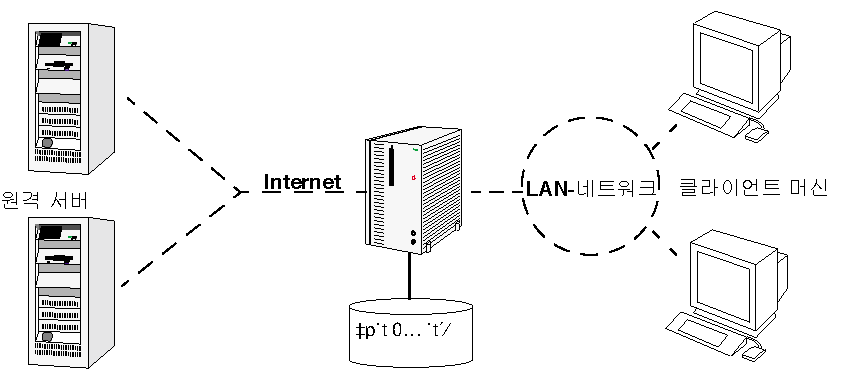
\includegraphics[width=\textwidth]{ArchitectureDiagram}
\caption{유지보수자와의 토론에서 유추한 아키텍처 다이어그램}
\figlabel{ArchitectureDiagram}
\end{center}
\end{figure}

사무실로 돌아와서 로컬 서버를 테스트하기 위한 명령 순서와 자동 거래 처리 및 여러 통화로 결제하기 위한 사용 시나리오가 포함된 간단한 보고서를 작성한다. 보고서에는 아키텍처 다이어그램(그림 6)과 다음과 같은 관찰 사항도 포함된다.

\begin{bulletlist}
  \item 인터넷 프로토콜 테스트는 수동으로 수행하여 회귀 테스트(regression test)에 대해 조사한다.

  \item 인터넷 프로토콜 사양은 독일 의료 보험 컨소시엄에서 제공받았다.

  \item 환자 목록 정렬해보고, 성 대신 이름 기준으로 정렬되는 것을 알았다.
\end{bulletlist}

\subsection*{근거}

\index{베넷, 사이몬}
\begin{quotation}
\noindent
\emph{``인터뷰 대상자의 답변에 유연하게 대응할 수 있는 능력은 인터뷰가 널리 사용되는 이유 중 하나이다.''}

\hfill --- 사이몬 베넷, \etal., \cite{Benn99a}

\index{넬슨, 제이콥}
\noindent
\emph{``인터뷰는 인터뷰 수행자가 상황에 맞게 인터뷰를 조정할 수 있기 때문에 아직 무엇을 찾고 있는지 모르는 탐색적 연구에 적합하다''}

\hfill --- 제이콥 넬슨, \cite{Niel93b}
\end{quotation}

소프트웨어 시스템을 사용하는 사람들을 인터뷰하는 것은 중요한 기능과 일반적인 사용 시나리오를 파악하는 데 필수적이다. 하지만 리엔지니어링 초기 단계에서는 무엇을 물어봐야 할지 모르기 때문에 미리 정의된 질문을 하는 것은 효과적이지 않다. 단순히 사람들이 시스템에 대해 어떤 점을 좋아하는지 물어보면 모호하거나 의미 없는 답변이 나올 수 있다. 게다가 사용자들은 레거시 시스템에 대해 불평하는 경향이 있기 때문에 매우 부정적인 답변을 얻을 위험이 있다. 

\index{골드버그, 아델}
\index{루빈, 케니}
\begin{quotation}
\noindent
\emph{``분석의 진정한 도전은 전문가가 다른 사람, 즉 분석가에게 개념을 전달해야 할 때 시작된다. 개념은 매우 풍부하고 광범위한 경우가 많기 때문에 일반적으로 전문가가 자신의 이해 전체를 하나의 총체적인 표현으로 적절하게 전달하는 것은 불가능하다.''}

\hfill --- 아델 골드버그, 케니 루빈, \cite{Gold95a}
\end{quotation}

포워드 엔지니어링 상황과 비교할 때 리버스 엔지니어는 작동 중인 소프트웨어 시스템이 있고 이를 활용할 수 있다는 한 가지 큰 장점이 있다. 이러한 상황에서는 데모를 요청하여 사용자에게 주도권을 넘기는 것이 안전하다. 우선, 데모를 통해 사용자는 자신의 말로 이야기를 전달할 수 있지만 데모는 일종의 유형적 구조를 부과하기 때문에 이해할 수 있다. 둘째, 사용자는 작동하는 시스템에서 시작해야 하기 때문에 무엇이 작동하는지 보다 긍정적인 태도로 설명할 수 있다. 마지막으로, 데모를 진행하는 동안 면접관은 정확한 질문을 많이 하고 정확한 답변을 얻을 수 있으므로 시스템 사용법에 대한 전문 지식을 파악할 수 있다.

\subsection*{알려진 용도}

이 패턴의 주요 아이디어인 사용자가 시스템을 사용하는 동안 시스템을 설명하게 하는 것은 일반적으로 사용자 인터페이스를 평가하는 데 사용된다. ``소리 내어 생각하기(Thinking aloud)는 가장 가치 있는 사용성 엔지니어링(usability engineering) 방법일 수 있다. 기본적으로 소리 내어 생각하기 테스트는 피험자가 지속적으로 큰 소리로 생각하면서 시스템을 사용하도록 하는 것이다.'' \cite{Niel93b} 요구사항 도출(requirements elicitation)을 위한 신속한 프로토타입 제작에도 동일한 아이디어가 종종 적용된다 \cite{Somm96a}.

\ind{FAMOOS} 프로젝트 초기의 한 일화에서는 이 패턴의 변형인 \variant{자신에게 직접 시연하기}를 적용하여 소프트웨어 시스템이 작동하는 것을 보고 무지한 질문이 어떻게 유지보수 팀 내에서 잠자고 있는 전문성을 촉발할 수 있는지를 보여준다. 사례 연구 중 하나인 데이터베이스 계층, 도메인 객체 계층, 사용자 인터페이스 계층으로 구성된 3계층 시스템(3-tiered system)의 전형적인 예로 '비즈니스 객체를 가져와야 한다'는 요청을 받았다. 두 명의 개인에게 이 작업을 맡겼는데, 한 사람은 소스 코드 브라우저와 CASE 도구를 사용하여 해당 비즈니스 객체를 나타내는 클래스 다이어그램을 추출했다. 다른 한 명은 로컬 PC에 시스템을 설치하고 약 한 시간 동안 사용자 인터페이스를 가지고 놀면서(즉, 시스템을 직접 시연하면서) 자신이 관찰한 몇 가지 이상한 점에 대한 10가지 질문 목록을 작성했다. 그 후, 시스템의 수석 분석가-설계자와 시스템을 리버스 엔지니어링하려고 시도한 두 사람과 함께 회의가 진행되었다. 분석가-설계자는 클래스 다이어그램을 보고 이것이 실제로 비즈니스 객체라는 것을 확인했지만, 뭔가 빠진 것이 있는지, 설계의 근거가 무엇인지에 대해서는 말해주지 않았다. 우리가 10가지 질문을 던지고 나서야 그는 설계 과정에서 직면한 문제에 대해 매우 열정적이고 매우 상세한 설명을 시작했고, 심지어 이야기 도중 클래스 다이어그램을 가리키기도 했다! 분석가 겸 디자이너의 이야기를 듣고 나서 소스코드에서 클래스 다이어그램을 추출한 사람의 첫 반응은 '이런, 소스코드에서 그런 걸 읽은 적이 없다'는 것이었다.

\subsection*{관련 패턴}

최종 사용자와 상호 작용하는 방법에 관한 많은 좋은 조언이 ``고객 상호 작용 패턴(Customer Interaction Patterns)'' \cite{Risi00a}에 구체화되어 있다. 이 패턴의 주요 메시지는 ``판매가 아닌 관계(It's a Relationship, Not a Sale)''라는 것으로, 최종 사용자와의 접점에서 신뢰 관계를 구축하는 것을 목표로 해야 한다는 점을 강조한다.

\subsection*{다음 단계}

최적의 결과를 얻으려면 여러 종류의 사람들과 \patref{데모 중 인터뷰하기}{InterviewDuringDemo}를 여러 번 시도해야 한다. 취향에 따라 이러한 시도를 \patref{한 시간 안에 모든 코드 읽기}{ReadAllTheCodeInOneHour} 및 \patref{문서 스키밍하기}{SkimTheDocumentation}의 전, 후 또는 혼합하여 수행할 수 있다. 그 후에는 \patref{유지보수자와 담소나누기}{ChatWithTheMaintainers}를 사용하여 일부 결과를 확인한다. 

시스템과의 첫 접촉이 끝나면 프로젝트를 어떻게 진행할지 (또는 취소할지) 결정해야 한다. 데모를 보면 사람들이 시스템을 어떻게 사용하는지, 어떤 기능을 높이 평가하는지에 대한 느낌을 알 수 있다. 따라서 소프트웨어 시스템의 중요한 부분과 리버스 엔지니어링이 필요한 부분을 알 수 있다. 사용 시나리오는 \patpgref{디자인에 대해 추측}{SpeculateAboutDesign} 및 \patpgref{비즈니스 규칙을 테스트로 기록}{RecordBusinessRulesAsTests}와 같은 패턴의 입력으로도 사용할 수 있다.

%=================================================================
%:PATTERN -- Do a Mock Installation
\pattern{모의 설치 수행하기}{DoAMockInstallation}

\intent{시스템을 설치하고 코드를 다시 컴파일하여 필요한 산출물을 사용할 수 있는지 확인한다.}

\subsection*{문제}

시스템을 (재)빌드할 수 있다는 것을 어떻게 확신할 수 있는가?

\emph{이 문제는 다음과 같은 이유로 어렵다.}

\begin{bulletlist}
  \item 여러분에게는 시스템이 새롭기 때문에 시스템을 빌드하는 데 필요한 파일을 모른다.

  \item 시스템이 라이브러리, 프레임워크, 패치에 의존할 수 있으며 올바른 버전을 사용할 수 있는지 확실하지 않다.

  \item 시스템이 크고 복잡하며 시스템이 실행되는 정확한 구성이 불분명하다.

  \item 유지보수자가 이러한 질문에 답하거나 설명서에서 답을 찾을 수 있지만 이 답변이 완전한지 확인해야 한다.
\end{bulletlist}

\emph{그러나 이 문제를 해결할 수 있는 이유는 다음과 같다.}

\begin{bulletlist}
  \item \emph{소스 코드(source code)}와 필요한 빌드 도구(예: 메이크파일, 컴파일러, 링커)에 접근할 수 있다.

  \item 실행 중인 시스템과 유사한 환경(예: 설치 CD 및 올바른 운영 체제가 설치된 컴퓨터)에서 시스템을 \emph{재설치(re-install)}할 수 있다.

  \item 시스템에 일종의 \emph{자체 테스트(self test)}가 포함되어 있을 수 있다. (\charef{테스트라는 생명 보험}{TestsYourLifeInsurance} 참조)를 사용하여 빌드 또는 설치가 성공했는지 확인할 수 있다.
\end{bulletlist}

\subsection*{솔루션}

제한된 시간(최대 하루) 동안 깨끗한 환경에서 시스템을 설치 및 빌드해 보자. 시스템에 자체 테스트가 포함되어 있으면 실행한다. 

\subsubsection*{힌트}

설치 및 빌드 프로세스를 완전히 이해하는 것이 아니라 다시 수행할 수 있는지 확인하는 것이 핵심이다.

빌드 및 설치 프로세스 중에 발생하는 모든 작은 오류와 해결 방법을 기록하면 시스템 구성과 라이브러리, 프레임워크 및 패치에 대한 종속성에 대해 알 수 있으므로 이를 기록하자. 예를 들어 특정 위치에서 시스템을 컴파일할 수 없거나 특정 컴퓨터에서만 액세스할 수 있는 오래된 레거시 라이브러리가 필요하거나 특정 라이브러리 패치가 필요하다는 사실을 알게 될 수 있다.

결국 시스템을 완전히 빌드하거나 설치하는 데 성공하지 못했을 수도 있다. 이는 리엔지니어링 프로젝트에 큰 영향을 미칠 가능성이 높은 위험에 해당하므로 계속 진행하기 전에 빌드 및 설치 절차를 연구하고 필요한 경우 이를 조정할 계획을 세워야 한다.

이 빌드 및 설치 실험이 끝나면 다음 내용이 포함된 보고서를 준비하자.

\begin{bulletlist}
  \item 사용된 라이브러리, 프레임워크 및 패치의 \emph{버전(version number)}

  \item 인프라(데이터베이스, 네트워크 툴킷, 포트, $\cdots$) 간의 \emph{종속성(dependency)}.

  \item 발생한 \emph{문제(problem)}와 해결 방법.

  \item \emph{개선(improvement)}에 대한 제안 사항.

  \item (불완전한 설치 또는 빌드의 경우) 솔루션 및 해결 방법의 가능성을 포함한 상황에 대한 \emph{평가(assessment)}.
\end{bulletlist}

\subsection*{트레이드오프}

\subsubsection*{장점}

\begin{bulletlist}
  \item \emph{필수 전제 조건.}
시스템을 (재)구축하거나 (재)설치할 수 있는 능력은 리엔지니어링 프로젝트에 필수적이므로 이 문제를 초기에 평가해야 한다. 구축 또는 설치가 어렵거나 불가능한 것으로 판명되면 필요한 수정 조치를 계획하자.

  \item \emph{정확성 요구.}
빌드 및 설치 프로세스를 복제하면 필요한 구성 요소에 대해 정확하게 파악해야 한다. 특히 마이그레이션 프로젝트의 경우 모든 구성 요소를 대상 플랫폼에서도 사용할 수 있어야 하므로 이 정보는 매우 중요하다.

  \item \emph{신뢰성을 높이기.}
빌드 또는 설치 후에는 어려운 단계를 직접 경험하게 된다. 개선에 대한 구체적인 제안을 쉽게 할 수 있어야 유지 관리 팀에 대한 신뢰도가 높아질 것이다.
\end{bulletlist}

\subsubsection*{단점}

\begin{bulletlist}
  \item \emph{지루한 활동.}
특히 대부분의 문제가 지금은 관심이 없는 사소한 세부 사항에 달려 있기 때문에 시스템 설치 실패의 원인을 추적하는 동안 매우 비생산적으로 느껴질 것이다. \patref{모의 설치 수행하기}{DoAMockInstallation}에 할애하는 시간을 제한하면 이 효과를 어느 정도 줄일 수 있지만, 그러면 시스템 구축이나 설치에 성공하지 못했기 때문에 더욱 비생산적으로 느껴질 것이다.

  \item \emph{불확실성.}
이 패턴은 정밀성을 요구하지만 일부 구성 요소를 재설계한 후 실제로 시스템 구축에 성공할 수 있다는 보장은 없다. 특히 신뢰할 수 있는 자체 테스트가 누락되면 빌드 또는 설치가 완료되었는지 확인할 수 없다.
\end{bulletlist}

\subsubsection*{어려움}

\begin{bulletlist}
  \item \emph{고민하지 않고 계속 시도하기.}
복잡한 시스템을 구축하거나 설치할 때 외부 요인(누락된 구성 요소, 불명확한 설치 스크립트)으로 인해 쉽게 실패할 수 있다. ``다음번에는 되겠지''라는 생각에 이런 성가신 문제를 계속 수정하고 싶은 유혹에 빠지기 쉽다. 이러한 세부 사항에 얽매이기보다는 시스템을 구축하는 것이 아니라 구축 프로세스에 대한 통찰력을 얻는다는 주요 목표를 놓치지 않는 것이 중요하다. 따라서 시간을 제한하고 발생하는 문제를 문서화하는 데 집중하여 나중에 문제를 해결할 수 있도록 해야 한다.
\end{bulletlist}

\subsection*{예시}

일부 최종 사용자와 \patref{데모 중 인터뷰}{InterviewDuringDemo}를 수행했으며, 그 결과 리엔지니어링 프로젝트에서 유지해야 할 중요한 기능에 대한 감을 잡았다. 하지만 프로젝트를 수락하기 전에 시스템을 변경할 수 있는지 여부를 확인해야 한다. 따라서 시스템을 새로 빌드할 수 있는지 확인하기 위해 간단한 실험을 해보기로 결정한다.

데이브가 사무실에 두고 간 상자에서 모든 소스 코드가 들어 있는 두 번째 CD를 가져온다. 디렉터리를 살펴보다가 최상위 메이크파일 하나를 발견하고 시도해 보기로 결정한다. 모든 파일을 시스템의 Linux 파티션에 복사하고 프롬프트에 \cmd{make all} 명령을 입력한다. 잠시 동안 모든 것이 순조롭게 진행되며 시스템은 수많은 자바 컴파일 성공을 보고한다. 하지만 안타깝게도 몇 분 후 \ct{java.sql} 라이브러리가 누락되어 make가 실패한다. JDK1.1이 설치되어 있다는 사실을 깨닫게 되지만, 문서에서 JDK1.3이 설치되어야 한다고 언급한 것을 기억한다. 마지못해 전체 디렉토리 구조를 휴지통에 버리고 JDK1.1을 제거한 다음 JDK1.3을 다운로드하여 설치한 다음(다운로드하는 데 시간이 오래 걸리므로 커피 한 잔을 가져와야 한다) 다시 시작한다. 이번에는 C 코드 컴파일이 시작될 때까지 메이크가 순조롭게 진행된다. 라이브러리 파일이 누락되어 첫 번째 컴파일이 즉시 실패하고 C 파일을 열어 이 실패의 원인이 정확히 무엇인지 확인합니다. assert.h는 시스템에서 사용할 수 있는 표준 라이브러리이므로 검색 경로에 문제가 있는 것이 분명하다. 그때는 거의 점심 시간이었고 오늘 이 빌드 실험을 끝내기로 계획했기 때문에 전체 C 컴파일은 나중에 하기로 결정했다. 어쨌든 데이브가 팀에 같이 있고, 그가 이 C 코드를 작성했으니 컴파일하는 방법을 보여줄 수 있을 것이다.

점심 식사 후에는 작성한 코드가 정상인지 확인하고 싶을 것이다. \lct{"void main("}를 grep하면 \emph{XDoctor}.java 파일에 메인 항목이 포함되어 있음을 알 수 있으므로 java \emph{XDoctor}를 입력하여 시스템을 실행한다. 실제로 데모에서 보셨던 시작 화면이 나타나고 \emph{``시스템이 데이터베이스에 연결 중입니다''}라는 작은 상태 창이 나타난다. 그 직후 \emph{``예상치 못한 일이 발생했습니다''} 메시지와 함께 시스템이 실패하고 데이터베이스 누락이 원인인 것으로 의심된다. 이 문제를 나중에 조사하기로 결정하고 설치 절차를 확인하기로 한다.

시스템을 설치할 수 있는지 확인하기 위해 설치 CD를 Macintosh의 CD 드라이브에 넣는다. 자동으로 일반적인 설치 창이 나타나고 설치 프로세스를 원활하게 진행한다. 설치 프로세스가 완료되면 설치 프로그램에서 시스템을 시작하기 전에 컴퓨터를 재부팅하라는 메시지가 표시된다. 어떤 시스템 확장 프로그램이 설치되었는지 확인하고 컴퓨터를 재부팅한 다음 바탕화면에 나타난 \emph{XDoctor} 아이콘을 더블 클릭한다. 안타깝게도 라이센스 키를 입력하라는 창이 나타납니다. CD 상자를 살펴보니 라이센스 키는 별도의 편지로 받았어야 하는데 당연히 받지 못했다. ``아쉽네, 라이선스 키가 제공되지 않았을 때 \emph{proDoc}처럼 시스템의 데모 버전을 실행할 수 있으면 좋았을 텐데'' 하는 생각이 든다. 좌절하여 포기하고 다음과 같은 보고서를 작성하기로 결정한다.

\begin{bulletlist}
  \item JDK1.3으로 make가 작동하는 것으로 보임: 이 빌드가 완료되었는지 확인할 수 없다.

  \item C 컴파일 실패: 데이브에게 빌드 데모를 요청한다.

  \item 라이선스 더 자세히 조사: 시스템이 어떻게 보호되는가?

  \item \emph{제안:}
라이선스 키가 제공되지 않으면 데모 모드로 실행한다(참조: \emph{proDoc}).

  \item \emph{제안:}
호출 시 사전 조건을 확인한다. \ct{XDoctor.main()}; 새로 빌드한 후 ``예기치 않은 일이 발생했다''라는 메시지와 함께 시스템이 종료된다.
\end{bulletlist}

\subsection*{알려진 용도}

\ind{FAMOOS} 사례 연구 중 하나에서는 중앙 서버와 소켓을 통해 통신하는 분산 시스템을 간단한 명령어를 사용하여 리엔지니어링해야 했다. 첨부된 편지에 따르면 ``필요한 모든 것이 들어 있는'' tar 파일이 들어 있는 테이프를 받았다. 그러나 시스템을 재구축하고 다시 설치하는 것이 어려웠고, 설치 스크립트를 자세히 살펴보고 관리자에게 설명을 요청해야 했다. 결국 보안 및 연결 문제로 인해 중앙 서버와 통신할 수는 없었지만 시뮬레이션 모드에서 시스템을 테스트할 수 있었다. 실험이 완전히 성공하지는 못했지만 시스템 아키텍처에 대한 인사이트를 얻을 수 있었다. 특히 시뮬레이션 모드가 중앙 서버를 모방하는 방식과 이것이 소스 코드와 메이크파일에 인코딩되는 방식은 나머지 프로젝트 기간 동안 중요한 정보를 제공했다.

우리가 수행한 감사 프로젝트의 첫날이 끝날 무렵, 다음 날 아침 새로 설치한 것을 보여 달라고 요청했다. 저희는 이를 \patref{데모 중 인터뷰하기}{InterviewDuringDemo}를 위한 준비를 위한 순수한 요청이라고 생각했지만, 설치 도중 한 명의 관리자가 설치 CD를 준비하기 위해 밤을 새워야 했다는 사실을 알게 되었다. 그 후의 토론을 통해 우리는 이 시스템이 사용자 기반이 고정되어 있고 인터넷을 통해 매주 업데이트를 다운로드하도록 설계된 시스템이라는 사실을 알게 되었다. 이는 이전에 \patref{한 시간 안에 모든 코드 읽기}{ReadAllTheCodeInOneHour}를 위해 노력하는 동안 관찰한 많은 특이한 점을 설명해 주었고, 남은 감사 프로젝트 동안 설계 문제를 드러내는 데 많은 도움이 되었다.

구성 관리 시스템(configuration management system)으로 작업할 때는 코드를 다시 컴파일하기 전에 먼저 코드를 깨끗한 구성으로 가져오는 것이 좋다. 예를 들어 \ind{Smalltalk} 시스템의 경우, 시스템을 구성하는 \ind{Envy} 구성 맵을 먼저 로드한 다음 코드를 깨끗한 이미지로 로드하는 것이 일반적인 조언 중 하나이다 \cite{Pelr01a}. 

\subsection*{다음 단계}

결론을 보고하기 전에 \patref{유지보수자와 담소나누기}{ChatWithTheMaintainers}를 하는 것이 좋다. 유지보수자는 여러분의 조사 결과를 확인하고 오해를 풀 수 있을 것이다. 개선에 대한 구체적인 제안은 관리자와 논의하는 것이 가장 좋은데, 이는 여러분이 진정으로 그들을 돕고자 하는 의지가 있음을 설득할 수 있는 가장 좋은 방법이기 때문이다.

빌드 또는 설치가 완전히 실패하는 경우 \patref{데모 중 인터뷰하기}{InterviewDuringDemo}를 \patref{모의 설치 수행하기}{DoAMockInstallation}와 결합하는 것이 좋다. 이 경우 유지보수자에게 빌드 또는 설치 프로세스를 시연해 달라고 요청하고 불분명한 단계에 대해 질문하자.

%=============================================================
\ifx\wholebook\relax\else
   \bibliographystyle{alpha}
   \bibliography{scg}
   \end{document}
\fi
%=============================================================

% $Author: oscar $
% $Date: 2013-11-27 16:48:27 +0100 (Wed, 27 Nov 2013) $
% $Revision: 35492 $
%=================================================================
\ifx\wholebook\relax\else
% --------------------------------------------
% Lulu:
	\documentclass[a4paper,10pt,twoside]{book}
	\usepackage[
		papersize={6.13in,9.21in},
		hmargin={.815in,.815in},
		vmargin={.98in,.98in},
		ignoreheadfoot
	]{geometry}
  \usepackage[hangul]{kotex}
	% $Author: oscar $
% $Date: 2009-09-13 20:58:29 +0200 (Sun, 13 Sep 2009) $
% $Revision: 29070 $
%=============================================================
% NB: documentclass must be set in main document.
% Allows book to be generated in multiple formats.
%=============================================================
%:Packages
\usepackage[T1]{fontenc}  %%%%%really important to get the code directly in the text!
\usepackage{palatino}
\usepackage{ifthen}
\usepackage{graphicx}
\graphicspath{{figures/}}
\usepackage{xspace}
\usepackage{makeidx}
\usepackage{isodateo} % enable \isodate
\usepackage{amssymb,textcomp}
%=============================================================
%:More packages
%\usepackage[english]{babel}
%\usepackage{lmodern}
%\usepackage[scaled=0.85]{helvet}
%\usepackage{microtype}
%\usepackage{theorem}
%\usepackage{float}
%\usepackage{longtable}
%\usepackage[nottoc]{tocbibind}
%\usepackage{multicol}
%\usepackage{booktabs}	% book-style tables
%\usepackage{topcapt}	% enables \topcaption
%\usepackage{multirow}
%\usepackage{tabularx}
%\usepackage{alltt}
\usepackage[usenames,dvipsnames]{color}
%\usepackage[hang]{subfigure}\makeatletter\def\p@subfigure{\thefigure\,}\makeatother
%\usepackage{rotating}
%\usepackage{enumitem}	% apb: allows more control over tags in enumerations
%\usepackage{verbatim}     % for comment environment
%\usepackage{varioref}	% for page references that work
%\usepackage{needspace}
%\usepackage[newparttoc]{titlesec}
%\usepackage{titletoc}
%\usepackage{wrapfig}
\usepackage[
	colorlinks=true,
	linkcolor=black,
	urlcolor=black,
	citecolor=black
]{hyperref}   % should come last
%=============================================================
%:URL style
\makeatletter
\def\url@leostyle{%
  \@ifundefined{selectfont}{\def\UrlFont{\sf}}{\def\UrlFont{\sffamily}}}
\makeatother
\urlstyle{leo}
%=============================================================
%:Booleans
\newboolean{lulu}
\setboolean{lulu}{false}
\newcommand{\ifluluelse}[2]{\ifthenelse{\boolean{lulu}}{#1}{#2}}
%=============================================================
%:Editorial comment macros
\newcommand{\nnbb}[2]{
  \fbox{\bfseries\sffamily\scriptsize#1}
  {\sf\small$\blacktriangleright$\textit{#2}$\blacktriangleleft$}
}
\newcommand{\on}[1]{\nnbb{Oscar}{#1}}
\newcommand{\here}{\nnbb{CONTINUE}{HERE}}
%=============================================================
%:Abbreviation macros
\newcommand{\ie}{\emph{i.e.},\xspace}
\newcommand{\eg}{\emph{e.g.},\xspace}
\newcommand{\etc}{\emph{etc.}\xspace}
\newcommand{\etal}{\emph{et al.}\xspace}
\newcommand{\straightquote}{"}
\newcommand{\sba}{\url{SquareBracketAssociates.org}\xspace}
%=============================================================
%:Patterns
% \newcommand{\pattern}[2]{\newpage\section{{\sf #1}}\label{pat:#2}}
% \newcommand{\pattern}[2]{\newpage\index{#1 (Pattern)}\section{#1}\label{pat:#2}}
\newcommand{\pattern}[2]{\cleardoublepage\index{#1 (패턴)}\section{#1}\label{pat:#2}}
\newcommand{\thumbnail}[2]{\index{#1 (패턴)}\subsection{#1}\label{pat:#2}}
\newcommand{\thumblang}[2]{\index{#1 (패턴 랭귀지)}\subsection{#1}\label{pat:#2}}
\newcommand{\variant}[1]{{\emph{#1}}\xspace}
% \newcommand{\problem}[1]{\subsection*{Problem}\emph{#1}}
\newcommand{\intent}[1]{\paragraph{의도}\emph{#1}}
\newcommand{\problem}[1]{\paragraph{문제}\emph{#1}}
\newcommand{\solution}[1]{\paragraph{해결}\emph{#1}}
\newcommand{\discussion}[0]{\paragraph{토론}}
\newcommand{\cmd}[1]{{\tt #1}\xspace}
%=============================================================
%:Environments
\newenvironment{bulletlist}{\begin{itemize}\setlength{\itemsep}{0ex}}
{\end{itemize}}
%=============================================================
%:Cross reference macros
\newcommand{\chalabel}[1]{\label{cha:#1}}
\newcommand{\seclabel}[1]{\label{sec:#1}}
\newcommand{\figlabel}[1]{\label{fig:#1}}
\newcommand{\tablabel}[1]{\label{tab:#1}}
\newcommand{\rulelabel}[1]{\label{rule:#1}}
\newcommand{\eglabel}[1]{\label{eg:#1}}
\newcommand{\scrlabel}[1]{\label{scr:#1}}
\newcommand{\mthlabel}[1]{\label{mth:#1}}
\newcommand{\clslabel}[1]{\label{cls:#1}}
\newcommand{\faqlabel}[1]{\label{faq:#1}}
%\newcommand{\charef}[1]{Chapter~\ref{cha:#1}\xspace}
%\newcommand{\secref}[1]{Section~\ref{sec:#1}\xspace}
\newcommand{\figref}[1]{Figure~\ref{fig:#1}\xspace}
% \newcommand{\patpgref}[2]{\hyperref[pat:#2]{\sf #1} [p.~\pageref{pat:#2}]\xspace}
\newcommand{\patpgref}[2]{\index{#1 (Pattern)}\hyperref[pat:#2]{#1} [p.~\pageref{pat:#2}]\xspace}
\newcommand{\patlangpgref}[2]{\index{#1 (Pattern language)}\hyperref[pat:#2]{#1} [p.~\pageref{pat:#2}]\xspace}
% \newcommand{\patref}[2]{\hyperref[pat:#2]{\sf #1}\xspace}
\newcommand{\patref}[2]{\index{#1 (Pattern)}\hyperref[pat:#2]{#1}\xspace}
\newcommand{\patlangref}[2]{\index{#1 (Pattern language)}\hyperref[pat:#2]{#1}\xspace}
% \newcommand{\charef}[2]{\hyperref[cha:#2]{\underline{\sf #1}}\xspace}
% \newcommand{\charef}[2]{\hyperref[cha:#2]{\sf #1}\xspace}
\newcommand{\charef}[2]{\index{#1 (Pattern cluster)}\hyperref[cha:#2]{#1}\xspace}
% \newcommand{\chapgref}[2]{\hyperref[cha:#2]{\sf #1} [p.~\pageref{cha:#2}]\xspace}
\newcommand{\chapgref}[2]{\index{#1 (Pattern cluster)}\hyperref[cha:#2]{#1} [p.~\pageref{cha:#2}]\xspace}
%\newcommand{\Figref}[1]{Figure~\ref{fig:#1}\xspace}
%\newcommand{\appref}[1]{Appendix~\ref{app:#1}\xspace}
%\newcommand{\tabref}[1]{Table~\ref{tab:#1}\xspace}
%\newcommand{\ruleref}[1]{\ref{rule:#1}\xspace}
%\newcommand{\egref}[1]{example~\ref{eg:#1}\xspace}
%\newcommand{\Egref}[1]{Example~\ref{eg:#1}\xspace}
%\newcommand{\scrref}[1]{script~\ref{scr:#1}\xspace}
%\newcommand{\Scrref}[1]{Script~\ref{scr:#1}\xspace}
%\newcommand{\tscrref}[1]{the script~\ref{scr:#1}\xspace}
%\newcommand{\Tscrref}[1]{The script~\ref{scr:#1}\xspace}
%\newcommand{\mthref}[1]{method~\ref{mth:#1}\xspace}
%\newcommand{\mthsref}[1]{methods~\ref{mth:#1}\xspace}
%\newcommand{\Mthref}[1]{Method~\ref{mth:#1}\xspace}
%\newcommand{\tmthref}[1]{the method~\ref{mth:#1}\xspace}
%\newcommand{\Tmthref}[1]{The method~\ref{mth:#1}\xspace}
%\newcommand{\clsref}[1]{class~\ref{cls:#1}\xspace}
%\newcommand{\tclsref}[1]{the class~\ref{cls:#1}\xspace}
%\newcommand{\Tclsref}[1]{The class~\ref{cls:#1}\xspace}
%=============================================================
%:Page Layout
\setlength{\headsep}{1cm}
%=============================================================
%:Menu item macro
%\definecolor{lightgray}{gray}{0.89}
%\newcommand{\menu}[1]{{%
%	\setlength{\fboxsep}{0pt}%
%	\colorbox{lightgray}{{{\upshape\sffamily\strut \,#1\,}}}}}
%\newcommand{\go}{\,$\triangleright$\,}
%\newcommand{\short}[1]{\mbox{{\sc cmd}\hspace{0.08em}--\hspace{0.09em}#1}\xspace}
%\newcommand{\button}[1]{{%
%	\setlength{\fboxsep}{0pt}%
%	\fbox{{\upshape\sffamily\strut \,#1\,}}}}
%\newcommand{\toolsflap}{\textit{Tools} flap\xspace}
%=============================================================
%:Section depth
%\setcounter{secnumdepth}{2}
%
%\DeclareGraphicsExtensions{.pdf, .jpg, .png}
%=============================================================
%:PDF setup
\hypersetup{
   pdftitle={Object-Oriented Reengineering Patterns},
   pdfauthor={Serge Demeyer, St\'ephane Ducasse, Oscar Nierstrasz},
   pdfkeywords={Reengineering, Object-Oriented Programming, Patterns},
   pdfsubject={Computer Science}
}
%=============================================================
%:Page layout and appearance
%\renewcommand{\chaptermark}[1]{\markboth{#1}{}}
%\renewcommand{\sectionmark}[1]{\markright{\thesection\ #1}}
%\renewpagestyle{plain}[\small\itshape]{%
%	\setheadrule{0pt}%
%	\sethead[][][]{}{}{}%
%	\setfoot[][][]{}{}{}}
%\renewpagestyle{headings}[\small\itshape]{%
%	\setheadrule{0pt}%
%	\setmarks{chapter}{section}%
%	\sethead[\thepage][][\chaptertitle]{\sectiontitle}{}{\thepage}%
%	\setfoot[][][]{}{}{}}
%=============================================================
%:Title section setup and TOC numbering depth
%\setcounter{secnumdepth}{1}
%\setcounter{tocdepth}{1}
%\titleformat{\part}[display]{\centering}{\huge\partname\ \thepart}{1em}{\Huge\textbf}[]
%\titleformat{\chapter}[display]{}{\huge\chaptertitlename\ \thechapter}{1em}{\Huge\raggedright\textbf}[]
%\titlecontents{part}[3pc]{%
%		\pagebreak[2]\addvspace{1em plus.4em minus.2em}%
%		\leavevmode\large\bfseries}
%	{\contentslabel{3pc}}{\hspace*{-3pc}}
%	{}[\nopagebreak]
%\titlecontents{chapter}[3pc]{%
%		\pagebreak[0]\addvspace{1em plus.2em minus.2em}%
%		\leavevmode\bfseries}
%	{\contentslabel{3pc}}{}
%	{\hfill\contentspage}[\nopagebreak]
%\dottedcontents{section}[3pc]{}{3pc}{1pc}
%\dottedcontents{subsection}[3pc]{}{0pc}{1pc}
%\let\origdoublepage\cleardoublepage
%\newcommand{\clearemptydoublepage}{%
%  \clearpage
%  {\pagestyle{empty}\origdoublepage}}
%\let\cleardoublepage\clearemptydoublepage % see http://www.tex.ac.uk/cgi-bin/texfaq2html?label=patch
%=============================================================
%:Listings package configuration
\newcommand{\caret}{\makebox{\raisebox{0.4ex}{\footnotesize{$\wedge$}}}}
% \newcommand{\escape}{{\sf \textbackslash}}
\definecolor{source}{gray}{0.95}
\usepackage{listings}
\lstdefinelanguage{Smalltalk}{
  morestring=[d]',
% Adapt this to other languages!
%  morecomment=[s]{"}{"},
  alsoletter={\#:},
  %escapechar={!},
  literate=
    {BANG}{!}1
%    {UNDERSCORE}{\_}1
    {\\st}{Smalltalk}9 % convenience -- in case \st occurs in code
    % {'}{{\textquotesingle}}1 % replaced by upquote=true in \lstset
%    {_}{{$\leftarrow$}}1
    {>>>}{{\sep}}1
    {^}{{$\uparrow$}}1
    {~}{{$\sim$}}1
    {-}{{\sf -\hspace{-0.13em}-}}1  % the goal is to make - the same width as +
    {+}{\raisebox{0.08ex}{+}}1		% and to raise + off the baseline to match -
    {-->}{{\quad$\longrightarrow$\quad}}3
	, % Don't forget the comma at the end!
  tabsize=4
}[keywords,comments,strings]

\lstset{language=Smalltalk,
	basicstyle=\sffamily,
	keywordstyle=\color{black}\bfseries,
	% stringstyle=\ttfamily, % Ugly! do we really want this? -- on
	mathescape=true,
	showstringspaces=false,
	keepspaces=true,
	breaklines=true,
	breakautoindent=true,
	backgroundcolor=\color{source},
	lineskip={-1pt}, % Ugly hack
	upquote=true, % straight quote; requires textcomp package
	columns=fullflexible} % no fixed width fonts
% \newcommand{\ct}{\lstinline[mathescape=false,basicstyle={\sffamily\upshape}]}
\newcommand{\ct}{\lstinline[mathescape=false,backgroundcolor=\color{white},basicstyle={\sffamily\upshape}]}
\newcommand{\lct}[1]{{\textsf{\textup{#1}}}}
%\newcommand{\scat}[1]{\emph{\textsf{#1}}\xspace}
%\newcommand{\prot}[1]{\emph{\textsf{#1}}\xspace}
% NB: No argument!
\lstnewenvironment{code}[0]{%
	\lstset{%
		% frame=lines,
		frame=single,
		framerule=0pt,
		mathescape=false
	}
}{}
%\def\ignoredollar#1{}
%=============================================================
%:Reserving space
%\newcommand{\needlines}[1]{\Needspace{#1\baselineskip}}
%=============================================================
%:Indexing macros
% Macros ending with "ind" generate text as well as an index entry
% Macros ending with "index" *only* generate an index entry
\newcommand{\ind}[1]{\index{#1}#1\xspace} % plain text
\newcommand{\subind}[2]{\index{#1!#2}#2\xspace} % show #2, subindex under #1
\newcommand{\emphind}[1]{\index{#1}\emph{#1}\xspace} % emph #1
\newcommand{\emphsubind}[2]{\index{#1!#2}\emph{#2}\xspace} % show emph #2, subindex under #1
\newcommand{\patind}[1]{\index{#1@#1 (pattern)}\ct{#1}\xspace} % pattern
\newcommand{\seeindex}[2]{\index{#1|see{#2}}} % #1, see #2
%\newcommand{\boldidx}[1]{{\bf #1}} % breaks hyperlink
%\newcommand{\indmain}[1]{\index{#1}#1\xspace} 
%\newcommand{\emphsubindmain}[2]{\index{#1!#2}\emph{#2}\xspace} % subindex, main entry
%\newcommand{\subindmain}[2]{\index{#1!#2}#2\xspace} % subindex, main entry
%\newcommand{\clsindmain}[1]{\index{#1!\#@(class)}\ct{#1}\xspace} % class main
%\newcommand{\indexmain}[1]{\index{#1}} 
%=============================================================
\parskip 1ex
%=============================================================

	\pagestyle{headings}
	\setboolean{lulu}{true}
% --------------------------------------------
% A4:
%	\documentclass[a4paper,11pt,twoside]{book}
%	% $Author: oscar $
% $Date: 2009-09-13 20:58:29 +0200 (Sun, 13 Sep 2009) $
% $Revision: 29070 $
%=============================================================
% NB: documentclass must be set in main document.
% Allows book to be generated in multiple formats.
%=============================================================
%:Packages
\usepackage[T1]{fontenc}  %%%%%really important to get the code directly in the text!
\usepackage{palatino}
\usepackage{ifthen}
\usepackage{graphicx}
\graphicspath{{figures/}}
\usepackage{xspace}
\usepackage{makeidx}
\usepackage{isodateo} % enable \isodate
\usepackage{amssymb,textcomp}
%=============================================================
%:More packages
%\usepackage[english]{babel}
%\usepackage{lmodern}
%\usepackage[scaled=0.85]{helvet}
%\usepackage{microtype}
%\usepackage{theorem}
%\usepackage{float}
%\usepackage{longtable}
%\usepackage[nottoc]{tocbibind}
%\usepackage{multicol}
%\usepackage{booktabs}	% book-style tables
%\usepackage{topcapt}	% enables \topcaption
%\usepackage{multirow}
%\usepackage{tabularx}
%\usepackage{alltt}
\usepackage[usenames,dvipsnames]{color}
%\usepackage[hang]{subfigure}\makeatletter\def\p@subfigure{\thefigure\,}\makeatother
%\usepackage{rotating}
%\usepackage{enumitem}	% apb: allows more control over tags in enumerations
%\usepackage{verbatim}     % for comment environment
%\usepackage{varioref}	% for page references that work
%\usepackage{needspace}
%\usepackage[newparttoc]{titlesec}
%\usepackage{titletoc}
%\usepackage{wrapfig}
\usepackage[
	colorlinks=true,
	linkcolor=black,
	urlcolor=black,
	citecolor=black
]{hyperref}   % should come last
%=============================================================
%:URL style
\makeatletter
\def\url@leostyle{%
  \@ifundefined{selectfont}{\def\UrlFont{\sf}}{\def\UrlFont{\sffamily}}}
\makeatother
\urlstyle{leo}
%=============================================================
%:Booleans
\newboolean{lulu}
\setboolean{lulu}{false}
\newcommand{\ifluluelse}[2]{\ifthenelse{\boolean{lulu}}{#1}{#2}}
%=============================================================
%:Editorial comment macros
\newcommand{\nnbb}[2]{
  \fbox{\bfseries\sffamily\scriptsize#1}
  {\sf\small$\blacktriangleright$\textit{#2}$\blacktriangleleft$}
}
\newcommand{\on}[1]{\nnbb{Oscar}{#1}}
\newcommand{\here}{\nnbb{CONTINUE}{HERE}}
%=============================================================
%:Abbreviation macros
\newcommand{\ie}{\emph{i.e.},\xspace}
\newcommand{\eg}{\emph{e.g.},\xspace}
\newcommand{\etc}{\emph{etc.}\xspace}
\newcommand{\etal}{\emph{et al.}\xspace}
\newcommand{\straightquote}{"}
\newcommand{\sba}{\url{SquareBracketAssociates.org}\xspace}
%=============================================================
%:Patterns
% \newcommand{\pattern}[2]{\newpage\section{{\sf #1}}\label{pat:#2}}
% \newcommand{\pattern}[2]{\newpage\index{#1 (Pattern)}\section{#1}\label{pat:#2}}
\newcommand{\pattern}[2]{\cleardoublepage\index{#1 (패턴)}\section{#1}\label{pat:#2}}
\newcommand{\thumbnail}[2]{\index{#1 (패턴)}\subsection{#1}\label{pat:#2}}
\newcommand{\thumblang}[2]{\index{#1 (패턴 랭귀지)}\subsection{#1}\label{pat:#2}}
\newcommand{\variant}[1]{{\emph{#1}}\xspace}
% \newcommand{\problem}[1]{\subsection*{Problem}\emph{#1}}
\newcommand{\intent}[1]{\paragraph{의도}\emph{#1}}
\newcommand{\problem}[1]{\paragraph{문제}\emph{#1}}
\newcommand{\solution}[1]{\paragraph{해결}\emph{#1}}
\newcommand{\discussion}[0]{\paragraph{토론}}
\newcommand{\cmd}[1]{{\tt #1}\xspace}
%=============================================================
%:Environments
\newenvironment{bulletlist}{\begin{itemize}\setlength{\itemsep}{0ex}}
{\end{itemize}}
%=============================================================
%:Cross reference macros
\newcommand{\chalabel}[1]{\label{cha:#1}}
\newcommand{\seclabel}[1]{\label{sec:#1}}
\newcommand{\figlabel}[1]{\label{fig:#1}}
\newcommand{\tablabel}[1]{\label{tab:#1}}
\newcommand{\rulelabel}[1]{\label{rule:#1}}
\newcommand{\eglabel}[1]{\label{eg:#1}}
\newcommand{\scrlabel}[1]{\label{scr:#1}}
\newcommand{\mthlabel}[1]{\label{mth:#1}}
\newcommand{\clslabel}[1]{\label{cls:#1}}
\newcommand{\faqlabel}[1]{\label{faq:#1}}
%\newcommand{\charef}[1]{Chapter~\ref{cha:#1}\xspace}
%\newcommand{\secref}[1]{Section~\ref{sec:#1}\xspace}
\newcommand{\figref}[1]{Figure~\ref{fig:#1}\xspace}
% \newcommand{\patpgref}[2]{\hyperref[pat:#2]{\sf #1} [p.~\pageref{pat:#2}]\xspace}
\newcommand{\patpgref}[2]{\index{#1 (Pattern)}\hyperref[pat:#2]{#1} [p.~\pageref{pat:#2}]\xspace}
\newcommand{\patlangpgref}[2]{\index{#1 (Pattern language)}\hyperref[pat:#2]{#1} [p.~\pageref{pat:#2}]\xspace}
% \newcommand{\patref}[2]{\hyperref[pat:#2]{\sf #1}\xspace}
\newcommand{\patref}[2]{\index{#1 (Pattern)}\hyperref[pat:#2]{#1}\xspace}
\newcommand{\patlangref}[2]{\index{#1 (Pattern language)}\hyperref[pat:#2]{#1}\xspace}
% \newcommand{\charef}[2]{\hyperref[cha:#2]{\underline{\sf #1}}\xspace}
% \newcommand{\charef}[2]{\hyperref[cha:#2]{\sf #1}\xspace}
\newcommand{\charef}[2]{\index{#1 (Pattern cluster)}\hyperref[cha:#2]{#1}\xspace}
% \newcommand{\chapgref}[2]{\hyperref[cha:#2]{\sf #1} [p.~\pageref{cha:#2}]\xspace}
\newcommand{\chapgref}[2]{\index{#1 (Pattern cluster)}\hyperref[cha:#2]{#1} [p.~\pageref{cha:#2}]\xspace}
%\newcommand{\Figref}[1]{Figure~\ref{fig:#1}\xspace}
%\newcommand{\appref}[1]{Appendix~\ref{app:#1}\xspace}
%\newcommand{\tabref}[1]{Table~\ref{tab:#1}\xspace}
%\newcommand{\ruleref}[1]{\ref{rule:#1}\xspace}
%\newcommand{\egref}[1]{example~\ref{eg:#1}\xspace}
%\newcommand{\Egref}[1]{Example~\ref{eg:#1}\xspace}
%\newcommand{\scrref}[1]{script~\ref{scr:#1}\xspace}
%\newcommand{\Scrref}[1]{Script~\ref{scr:#1}\xspace}
%\newcommand{\tscrref}[1]{the script~\ref{scr:#1}\xspace}
%\newcommand{\Tscrref}[1]{The script~\ref{scr:#1}\xspace}
%\newcommand{\mthref}[1]{method~\ref{mth:#1}\xspace}
%\newcommand{\mthsref}[1]{methods~\ref{mth:#1}\xspace}
%\newcommand{\Mthref}[1]{Method~\ref{mth:#1}\xspace}
%\newcommand{\tmthref}[1]{the method~\ref{mth:#1}\xspace}
%\newcommand{\Tmthref}[1]{The method~\ref{mth:#1}\xspace}
%\newcommand{\clsref}[1]{class~\ref{cls:#1}\xspace}
%\newcommand{\tclsref}[1]{the class~\ref{cls:#1}\xspace}
%\newcommand{\Tclsref}[1]{The class~\ref{cls:#1}\xspace}
%=============================================================
%:Page Layout
\setlength{\headsep}{1cm}
%=============================================================
%:Menu item macro
%\definecolor{lightgray}{gray}{0.89}
%\newcommand{\menu}[1]{{%
%	\setlength{\fboxsep}{0pt}%
%	\colorbox{lightgray}{{{\upshape\sffamily\strut \,#1\,}}}}}
%\newcommand{\go}{\,$\triangleright$\,}
%\newcommand{\short}[1]{\mbox{{\sc cmd}\hspace{0.08em}--\hspace{0.09em}#1}\xspace}
%\newcommand{\button}[1]{{%
%	\setlength{\fboxsep}{0pt}%
%	\fbox{{\upshape\sffamily\strut \,#1\,}}}}
%\newcommand{\toolsflap}{\textit{Tools} flap\xspace}
%=============================================================
%:Section depth
%\setcounter{secnumdepth}{2}
%
%\DeclareGraphicsExtensions{.pdf, .jpg, .png}
%=============================================================
%:PDF setup
\hypersetup{
   pdftitle={Object-Oriented Reengineering Patterns},
   pdfauthor={Serge Demeyer, St\'ephane Ducasse, Oscar Nierstrasz},
   pdfkeywords={Reengineering, Object-Oriented Programming, Patterns},
   pdfsubject={Computer Science}
}
%=============================================================
%:Page layout and appearance
%\renewcommand{\chaptermark}[1]{\markboth{#1}{}}
%\renewcommand{\sectionmark}[1]{\markright{\thesection\ #1}}
%\renewpagestyle{plain}[\small\itshape]{%
%	\setheadrule{0pt}%
%	\sethead[][][]{}{}{}%
%	\setfoot[][][]{}{}{}}
%\renewpagestyle{headings}[\small\itshape]{%
%	\setheadrule{0pt}%
%	\setmarks{chapter}{section}%
%	\sethead[\thepage][][\chaptertitle]{\sectiontitle}{}{\thepage}%
%	\setfoot[][][]{}{}{}}
%=============================================================
%:Title section setup and TOC numbering depth
%\setcounter{secnumdepth}{1}
%\setcounter{tocdepth}{1}
%\titleformat{\part}[display]{\centering}{\huge\partname\ \thepart}{1em}{\Huge\textbf}[]
%\titleformat{\chapter}[display]{}{\huge\chaptertitlename\ \thechapter}{1em}{\Huge\raggedright\textbf}[]
%\titlecontents{part}[3pc]{%
%		\pagebreak[2]\addvspace{1em plus.4em minus.2em}%
%		\leavevmode\large\bfseries}
%	{\contentslabel{3pc}}{\hspace*{-3pc}}
%	{}[\nopagebreak]
%\titlecontents{chapter}[3pc]{%
%		\pagebreak[0]\addvspace{1em plus.2em minus.2em}%
%		\leavevmode\bfseries}
%	{\contentslabel{3pc}}{}
%	{\hfill\contentspage}[\nopagebreak]
%\dottedcontents{section}[3pc]{}{3pc}{1pc}
%\dottedcontents{subsection}[3pc]{}{0pc}{1pc}
%\let\origdoublepage\cleardoublepage
%\newcommand{\clearemptydoublepage}{%
%  \clearpage
%  {\pagestyle{empty}\origdoublepage}}
%\let\cleardoublepage\clearemptydoublepage % see http://www.tex.ac.uk/cgi-bin/texfaq2html?label=patch
%=============================================================
%:Listings package configuration
\newcommand{\caret}{\makebox{\raisebox{0.4ex}{\footnotesize{$\wedge$}}}}
% \newcommand{\escape}{{\sf \textbackslash}}
\definecolor{source}{gray}{0.95}
\usepackage{listings}
\lstdefinelanguage{Smalltalk}{
  morestring=[d]',
% Adapt this to other languages!
%  morecomment=[s]{"}{"},
  alsoletter={\#:},
  %escapechar={!},
  literate=
    {BANG}{!}1
%    {UNDERSCORE}{\_}1
    {\\st}{Smalltalk}9 % convenience -- in case \st occurs in code
    % {'}{{\textquotesingle}}1 % replaced by upquote=true in \lstset
%    {_}{{$\leftarrow$}}1
    {>>>}{{\sep}}1
    {^}{{$\uparrow$}}1
    {~}{{$\sim$}}1
    {-}{{\sf -\hspace{-0.13em}-}}1  % the goal is to make - the same width as +
    {+}{\raisebox{0.08ex}{+}}1		% and to raise + off the baseline to match -
    {-->}{{\quad$\longrightarrow$\quad}}3
	, % Don't forget the comma at the end!
  tabsize=4
}[keywords,comments,strings]

\lstset{language=Smalltalk,
	basicstyle=\sffamily,
	keywordstyle=\color{black}\bfseries,
	% stringstyle=\ttfamily, % Ugly! do we really want this? -- on
	mathescape=true,
	showstringspaces=false,
	keepspaces=true,
	breaklines=true,
	breakautoindent=true,
	backgroundcolor=\color{source},
	lineskip={-1pt}, % Ugly hack
	upquote=true, % straight quote; requires textcomp package
	columns=fullflexible} % no fixed width fonts
% \newcommand{\ct}{\lstinline[mathescape=false,basicstyle={\sffamily\upshape}]}
\newcommand{\ct}{\lstinline[mathescape=false,backgroundcolor=\color{white},basicstyle={\sffamily\upshape}]}
\newcommand{\lct}[1]{{\textsf{\textup{#1}}}}
%\newcommand{\scat}[1]{\emph{\textsf{#1}}\xspace}
%\newcommand{\prot}[1]{\emph{\textsf{#1}}\xspace}
% NB: No argument!
\lstnewenvironment{code}[0]{%
	\lstset{%
		% frame=lines,
		frame=single,
		framerule=0pt,
		mathescape=false
	}
}{}
%\def\ignoredollar#1{}
%=============================================================
%:Reserving space
%\newcommand{\needlines}[1]{\Needspace{#1\baselineskip}}
%=============================================================
%:Indexing macros
% Macros ending with "ind" generate text as well as an index entry
% Macros ending with "index" *only* generate an index entry
\newcommand{\ind}[1]{\index{#1}#1\xspace} % plain text
\newcommand{\subind}[2]{\index{#1!#2}#2\xspace} % show #2, subindex under #1
\newcommand{\emphind}[1]{\index{#1}\emph{#1}\xspace} % emph #1
\newcommand{\emphsubind}[2]{\index{#1!#2}\emph{#2}\xspace} % show emph #2, subindex under #1
\newcommand{\patind}[1]{\index{#1@#1 (pattern)}\ct{#1}\xspace} % pattern
\newcommand{\seeindex}[2]{\index{#1|see{#2}}} % #1, see #2
%\newcommand{\boldidx}[1]{{\bf #1}} % breaks hyperlink
%\newcommand{\indmain}[1]{\index{#1}#1\xspace} 
%\newcommand{\emphsubindmain}[2]{\index{#1!#2}\emph{#2}\xspace} % subindex, main entry
%\newcommand{\subindmain}[2]{\index{#1!#2}#2\xspace} % subindex, main entry
%\newcommand{\clsindmain}[1]{\index{#1!\#@(class)}\ct{#1}\xspace} % class main
%\newcommand{\indexmain}[1]{\index{#1}} 
%=============================================================
\parskip 1ex
%=============================================================

%	\usepackage{a4wide}
% --------------------------------------------
	\begin{document}
	\renewcommand{\nnbb}[2]{} % Disable editorial comments
	\sloppy
\fi
%=================================================================
\chapter{초기 이해}
\chalabel{InitialUnderstanding}

여러분의 회사는 의사들이 사용할 수 있는 \emph{proDoc}이라는 의료 정보 시스템을 개발하여 제공하고 있다. 이제 회사는 다양한 의료 보험 회사와 거래를 수행하기 위해 인터넷 지원을 제공하는 경쟁 소프트웨어 \emph{XDoctor} 제품을 인수했다. 두 제품을 하나의 시스템으로 통합해야 한다.

\emph{XDoctor}를 처음 평가한 결과, 몇 가지 컴포넌트를 복구하여 통합해야 한다는 사실이 밝혀졌다. 물론 소프트웨어 컴포넌트를 성공적으로 복구하려면 내부 구조와 나머지 시스템과의 연결을 이해해야 한다. 예를 들어, 여러분의 회사는 고객에게 ``단 1바이트의 데이터도 손실되지 않는다''고 약속했으므로 데이터베이스 내용을 복구하고 결과적으로 데이터베이스 구조와 상위 계층이 데이터베이스에 어떻게 의존하는지 이해해야 한다. 또한 귀사는 건강 보험 회사와의 거래 지원을 지속하고 확대하겠다고 약속했으므로 이러한 원격 서비스와 통신하는 데 사용되는 네트워크 통신 컴포넌트를 복구해야 한다.

\subsection*{포스: 주요한 요구사항}

리엔지니어링 프로젝트에서 이와 유사한 상황이 자주 발생한다. 시스템 및 사용자와의 \chapgref{첫 번째 접근}{FirstContact}을 통해 어떤 기능이 가치가 있고 왜 복구해야 하는지 명확하게 알 수 있다. 하지만 소프트웨어 시스템의 전반적인 설계에 대한 지식이 부족하기 때문에 이 기능을 레거시 시스템에서 제거할 수 있는지 여부와 이에 소요되는 비용을 예측할 수 없다. 이러한 초기 이해는 리엔지니어링 프로젝트의 성공을 위해 매우 중요하며, 이 장에서는 이를 얻는 방법을 설명한다.

\charef{첫 번째 접근}{FirstContact}의 패턴을 통해 소프트웨어 시스템에 대한 첫 번째 아이디어를 얻는 데 도움이 되었을 것이다. 이제 이러한 아이디어를 초기 이해로 구체화하고 추가 리버스 엔지니어링 활동을 지원하기 위해 이러한 이해를 문서화할 때이다. 리버스 엔지니어링의 이 단계에서 가장 중요한 우선 순위는 나머지 프로젝트의 안정적인 기반을 구축하는 것이므로 발견한 내용이 정확하고 적절하게 문서화되어 있는지 확인해야 한다.

발견한 내용을 올바르게 문서화하는 방법은 프로젝트의 범위와 팀의 규모에 따라 크게 달라진다. 10명 이상의 개발자가 참여하는 복잡한 리버스 엔지니어링 프로젝트에는 몇 가지 표준 문서 템플릿과 구성 관리 시스템이 필요하다. 반면에 3인 미만이 참여하는 평범한 프로젝트는 중앙 서버에서 공유되는 느슨한 구조의 파일로 충분히 관리할 수 있다. 하지만 모든 상황에 적용되는 몇 가지 내재적인 포스(force)이 있다.

\begin{bulletlist}
\item \emph{데이터는 기만적이다.}
기존 소프트웨어 시스템을 이해하려면 데이터를 수집하고 해석하여 일관된 시각으로 요약해야 한다. 일반적으로 데이터를 해석하는 방법에는 두 가지 이상의 방법이 있으며, 대안 중에서 선택할 때 항상 구체적인 증거가 뒷받침되지 않는 가정을 하게 된다. \emph{따라서 정보의 출처를 다시 확인하여 탄탄한 토대 위에 이해를 구축해야 한다.}

\item \emph{이해는 반복이 필요하다.}
이해는 인간의 두뇌 내부에서 일어나므로 일종의 학습 과정에 해당하다. 리버스 엔지니어링 기술은 우리의 두뇌가 새로운 아이디어를 받아들이는 방식을 지원해야 하므로 매우 유연해야 하고 많은 반복과 역추적(backtracking)을 허용해야 한다. \emph{따라서 학습 과정을 자극하기 위해 반복(iteration)과 피드백 루프(feedback loop)를 계획해야 한다.}

\item \emph{지식을 공유해야 한다.}
시스템을 이해했다면 이 지식을 동료들과 공유하는 것이 중요하다. 동료가 업무를 수행하는 데 도움이 될 뿐만 아니라 여러분의 이해도를 높일 수 있는 의견과 피드백도 얻을 수 있다. \emph{따라서 벽에 지도를 붙이자.} 발견한 내용을 잘 보이는 곳에 게시하고 피드백에 대한 명시적인 규정을 마련하자. 이를 수행하는 방법은 팀 조직과 업무 습관에 따라 달라진다. 일반적으로 팀 회의는 정보를 공유하는 좋은 방법이지만(\patpgref{원탁 회의에 말하기}{SpeakToTheRoundTable} 참조), 커피 머신 근처의 벽에 큰 그림을 붙이는 것도 좋은 방법일 수 있다.

\item \emph{팀은 소통이 필요하다.}
시스템에 대한 이해를 구축하고 문서화하는 것은 목표가 아니라 목표를 달성하기 위한 수단이다. 시스템을 이해하기 위한 진정한 목표는 프로젝트에 참여하는 다른 사람들과 효과적으로 소통하는 것이므로, 이해한 것을 문서화하는 방식은 그 목표를 뒷받침해야 한다. 예를 들어 동료가 엔터티 관계 다이어그램(Entity-Relationship diagram)을 읽을 줄만 안다면 UML 클래스 다이어그램을 그릴 필요가 없고, 최종 사용자가 그 범위를 이해할 수 없다면 사용 사례를 작성하는 것도 의미가 없다. \emph{결국, 팀원이 사용하는 언어를 사용하자.} 팀원들이 여러분이 문서화한 내용을 읽고, 이해하고, 댓글을 달 수 있도록 여러분이 이해한 내용을 문서화할 언어를 선택하자.
\end{bulletlist}

\subsection*{개요}

소프트웨어 시스템을 처음 이해할 때 가장 우려되는 것은 잘못된 정보이다. 따라서 이러한 패턴은 신뢰할 수 있는 유일한 정보 소스인 소스 코드에 주로 의존한다.

원칙적으로 소스 코드를 연구하는 방법에는 하향식(top-down)과 상향식(bottom-up)의 두 가지 접근 방식이 있다. 실제로 모든 리버스 엔지니어링 접근 방식은 이 두 가지를 조금씩 모두 사용해야 하지만, 그래도 구분할 가치가 있다. 하향식 접근 방식에서는 높은 수준의 표현에서 시작하여 소스 코드와 비교하여 검증한다(예: \patref{디자인 추측하기}{SpeculateAboutDesign}의 설명 참조). 상향식 접근 방식에서는 소스 코드에서 시작하여 관련성이 있는 것을 필터링하고 관련 엔티티를 상위 수준 표현으로 캐스팅한다. 이 접근 방식은 \patref{퍼시스턴트 데이터 분석하기}{AnalyzeThePersistentData} 및 \patref{예외적인 엔티티 연구하기}{StudyTheExceptionalEntities}에서 사용된다.

이러한 각 패턴을 적용하는 데 선호되는 순서는 없다. 먼저 \patref{퍼시스턴트 데이터 분석하기}{AnalyzeThePersistentData}을 수행한 다음, \patref{디자인 추측하기}{SpeculateAboutDesign}을 통해 결과 모델을 구체화하고 마지막으로 이 지식을 활용하여 \patref{예외적인 엔티티 연구하기}{StudyTheExceptionalEntities}를 수행하는 것이 당연할 수 있다. 따라서 패턴은 이러한 순서로 표시된다. 그러나 시스템의 많은 부분이 데이터베이스와 관련이 없을 경우(일부 시스템에는 어떤 형태의 퍼시스턴트 데이터도 없다) 데이터베이스를 학습하지 않은 상태에서 \patref{디자인 추측하기}{SpeculateAboutDesign}을 수행해야 한다. 그리고 \patref{디자인 추측하기}{SpeculateAboutDesign}으로 시작하기 어려운 상황이라면 \patref{예외적인 엔티티 연구하기}{StudyTheExceptionalEntities}가 초기 가설을 제시해 줄 것이다.

\begin{figure}
\begin{center}
\includegraphics[width=\textwidth]{InitialUnderstandingMap}
\caption{소프트웨어 시스템의 \charef{초기 이해}{InitialUnderstanding}를 구하고 이를 상위 수준의 표현으로 변환한다.}
\figlabel{InitialUnderstandingMap}
\end{center}
\end{figure}

이러한 각 패턴에 할애해야 하는 시간은 리엔지니어링 프로젝트의 목표에 따라 크게 달라진다. 원칙적으로 이러한 패턴 중 어느 것도 오래 걸리지 않지만 각 패턴은 여러 번 적용해야 한다. 팀이 나머지 프로젝트를 진행할 만큼 충분히 이해했는지 여부는 패턴을 적용한 후에야 평가할 수 있기 때문에 얼마나 많은 주기가 필요할지 예측할 수 없다. 따라서 이러한 패턴은 사례별로 적용해야 한다.

\subsection*{다음 단계}

여러분이 추가로 이해한 내용을 프로젝트 계획에 반영해야 한다. 예를 들어 \patref{퍼시스턴트 데이터 분석하기}{AnalyzeThePersistentData} 및 \patref{디자인에 대한 추측}{SpeculateAboutDesign}은 시스템의 일부를 문서화하며, 이 문서를 기회(Opportunity)로 사용해야 한다. 반면에 \patref{예외적인 엔티티 연구하기}{StudyTheExceptionalEntities}를 사용하면 의심스러운 컴포넌트를 발견할 수 있으며, 이러한 컴포넌트는 리스크(Risk)로 관리해야 한다.

여러분이 충분히 이해하여 충분한 기초를 마련했다면 나머지 프로젝트에 중요한 컴포넌트에 대한 세부 정보를 채워 넣어야 한다. \chapgref{디테일 모델 캡처}{DetailedModelCapture}에 설명된 활동이 이러한 세부 정보를 채우는 데 도움이 될 수 있다.

%=================================================================
%:PATTERN -- {Analyze the Persistent Data}
\pattern{퍼시스턴트 데이터 분석하기}{AnalyzeThePersistentData}

\intent{데이터베이스 시스템 내부에 보관해야 할 정도로 중요한 개체에 대해 학습한다.}

\subsection*{문제}

Which object structures represent the valuable data ?
어떤 개체 구조가 중요한 데이터를 나타낼까요?

\emph{이 문제는 다음과 같은 이유로 어렵다.}

\begin{bulletlist}
\item 귀중한 데이터는 외부 저장 장치(예: 파일 시스템, \ind{database})에 안전하게 보관해야 한다. 그러나 이러한 데이터 저장소는 종종 다락방(attic)\footnote{서양에서는 오래된 물건을 다락방에 보관하곤 한다. -옮긴이} 역할을 하므로 거의 정리되지 않고 많은 정크를 포함할 수 있다.

\item 메모리에 로드될 때 중요한 데이터는 복잡한 객체 구조로 표현된다. 안타깝게도 외부 저장 장치에서 제공하는 데이터 구조와 주 메모리에 있는 객체 구조 사이에는 큰 차이가 있다. 예를 들어 상속 관계는 레거시 데이터베이스에서 명시적으로 제공되는 경우가 거의 없다.

\item ``값(Valuable)''은 상대적인 속성이다. 저장된 데이터의 상당 부분이 리엔지니어링 프로젝트와 관련이 없을 수 있다.
\end{bulletlist}

\emph{그러나 이 문제를 해결할 수 있는 이유는 다음과 같다.}

\begin{bulletlist}
\item 소프트웨어 시스템은 데이터를 영구적으로 유지하기 위해 어떤 형태의 데이터베이스를 사용합한. 따라서 데이터베이스 내부의 데이터에 대한 정적 설명을 제공하는 일종의 데이터베이스 스키마가 존재한다.

\item 데이터베이스에는 데이터베이스 내부의 실제 개체를 검사하는 데 필요한 도구가 함께 제공되므로 레거시 데이터의 존재를 활용하여 결과를 미세 조정할 수 있다.

\index{데이터베이스!스키마}
\item 구현 언어의 데이터 구조를 데이터베이스 스키마에 매핑하는 데 어느 정도 전문 지식이 있으며, 데이터베이스 스키마에서 클래스 다이어그램을 재구성할 수 있을 정도이다.

\item 시스템의 기능과 프로젝트의 목표를 대략적으로 이해하고 있으므로(예: \charef{첫 번째 접근}{FirstContact}를 통해 얻은 정보) 데이터베이스의 어느 부분이 프로젝트에 유용한지 평가할 수 있다.
\end{bulletlist}

\subsection*{해결}

데이터베이스 스키마를 분석하여 어떤 구조가 가치 있는 데이터를 나타내는지 필터링한다. 나머지 팀원들을 위해 해당 지식을 문서화할 수 있도록 해당 엔티티를 나타내는 \subind{UML}{클래스 다이어그램}을 도출한다.

\subsubsection*{단계}

아래 단계에서는 시스템이 객체 지향 애플리케이션의 일반적인 경우인 \emph{관계형 데이터베이스(relational database)}를 사용한다고 가정한다. 그러나 다른 종류의 데이터베이스 시스템을 사용하는 경우에도 이러한 단계 중 많은 부분이 여전히 적용될 수 있다. 단계 자체는 가이드라인일 뿐이므로 직관과 역추적을 충분히 활용하여 반복적으로 적용해야 한다.

\noindent
\emph{준비.}
관계형 데이터베이스 스키마에서 클래스 다이어그램을 도출하려면 먼저 테이블을 클래스로 표현하는 초기 모델을 준비한다. 소프트웨어 도구를 사용하여 이 작업을 수행할 수도 있지만 인덱스 카드 세트를 사용하는 것도 좋다.

\begin{enumerate}
  \item 모든 테이블 이름을 열거하고 각 테이블에 대해 같은 이름의 클래스를 만든다.

  \item 각 테이블에 대해 모든 열 이름을 수집하고 이를 해당 클래스에 속성으로 추가한다.

  \item 각 테이블에 대해 후보 키(candidate key)를 결정한다. 그중 일부는 데이터베이스 스키마에서 직접 읽을 수 있지만 일반적으로 더 자세한 분석이 필요하다. 후보 키를 제안하는 경우가 많으므로 모든 (고유) 인덱스를 반드시 확인하자. 명명 규칙(ID 또는 \#을 포함한 이름)도 후보 키를 나타낼 수 있다. 의심스러운 경우 데이터 샘플을 수집하여 후보 키가 데이터베이스 모집단 내에서 실제로 고유한지 확인한다.

  \item 테이블 간의 모든 외래 키(foreign key) 관계를 수집하고 해당 클래스 간의 연결을 생성한다. 외래 키 관계는 데이터베이스 스키마에 명시적으로 유지되지 않을 수 있으므로 열 유형과 명명 규칙(naming convention)을 통해 이를 유추해야 한다. 여기에는 동음이의어(homonym)(=열 이름과 유형은 동일하지만 의미는 다른)와 동의어(synonym)(=열 이름이나 유형은 다르지만 의미는 동일한)가 존재할 수 있으므로 신중한 분석이 필요하다. 이러한 어려움에 대처하려면 최소한 인덱스와 뷰 선언이 빈번한 탐색 경로를 가리키므로 이를 확인해야 한다. 가능하면 데이터베이스에 대해 실행되는 \ind{SQL} 문의 조인 절(join clause)을 확인한다. 마지막으로, 데이터 샘플을 검사하여 특정 외래 키 관계를 확인(verify)하거나 반박(refute)한다.

\end{enumerate}

\begin{figure}
\begin{center}
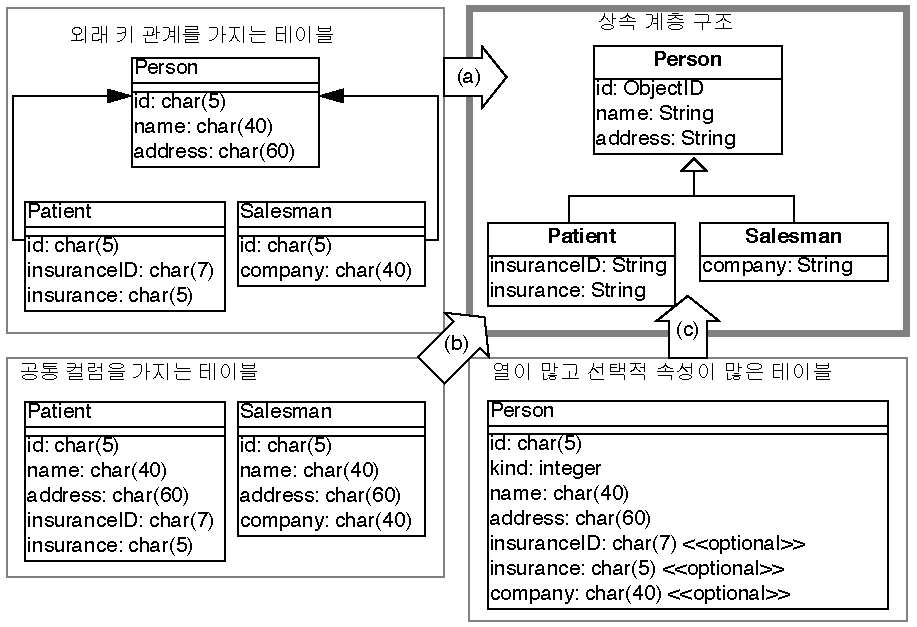
\includegraphics[width=\textwidth]{InitialMappingRelations}
\caption{계열 관계형 테이블을 상속 계층 구조에 매핑하기. (a) 일대일, (b) 롤다운, (c) 롤업}
\figlabel{InitialMappingRelations}
\end{center}
\end{figure}

\noindent
\emph{상속 통합(Incorporate inheritance).}
위의 단계를 마치면 관계형 데이터베이스에 저장되는 테이블을 나타내는 클래스 집합을 갖게 된다. 그러나 관계형 데이터베이스는 상속 관계를 나타낼 수 없기 때문에 외래 키에서 상속 관계를 유추해야 한다. (5-7단계에서 상속 관계의 세 가지 표현에 대한 용어는 \cite{Fros94a}에서 유래했다.)

\begin{enumerate}\setcounter{enumi}{4}
  \item \emph{일대일(One to one)} (\figref{InitialMappingRelations} (a)). 기본 키가 다른 테이블의 외래 키 역할도 하는 테이블을 확인한다. 이러한 외래 키는 상속 관계를 나타낼 수 있기 때문이다. 이러한 테이블에 대해 실행되는 SELECT 문을 검사하여 일반적으로 이 외래 키에 대한 조인을 포함하는지 확인한다. 이 경우 테이블 이름과 해당 소스 코드를 분석하여 이 외래 키가 실제로 상속 관계를 나타내는지 확인한다. 그렇다면 외래 키에 해당하는 연결을 상속 관계로 변환한다.

  \item \emph{롤다운(Rolled down)} (\figref{InitialMappingRelations} (b)). 클래스 계층 구조가 여러 테이블에 분산되어 있고 각 테이블이 하나의 비추상 클래스를 나타내는 상황을 나타낼 수 있으므로 열 정의의 공통 집합이 있는 테이블을 확인한다. 중복된 열 정의의 각 클러스터에 대해 공통 수퍼클래스를 정의하고 해당 속성을 새 클래스 내부로 이동한다. 소스 코드에서 새로 생성된 클래스에 적용할 수 있는 이름을 확인한다.

  \item \emph{롤업(Rolled up)} (\figref{InitialMappingRelations} (c)). 열이 많고 선택적 속성이 많은 테이블은 전체 클래스 계층 구조가 단일 테이블에 표시되는 상황을 나타낼 수 있으므로 확인한다. 이러한 테이블을 발견한 경우 이 테이블에 대해 실행되는 모든 SELECT 문을 검토한다. 이러한 SELECT 문이 명시적으로 열의 하위 집합을 요청하는 경우 요청된 하위 집합에 따라 이 하나의 클래스를 여러 클래스로 나눌 수 있다. 이러한 클래스의 이름에 대해 열거형 유형 번호를 포함하는 'kind' 열과 같은 하위 유형 정보의 인코딩이 있는지 확인한다.

\end{enumerate}

\noindent
\emph{연관 통합(Incorporate associations).}
데이터베이스에서 추출한 클래스 다이어그램이 너무 작을 수 있다. 실제 상속 계층 구조의 클래스가 새로운 속성을 정의하지 않아 데이터베이스에서 누락되었을 수 있다. 또한 테이블 및 열 이름이 이상하게 들릴 수도 있다. 따라서 클래스 다이어그램을 소스 코드와 비교하여 확인하면 추가적인 인사이트를 얻을 수 있으므로(\patref{디자인 추측하기}{SpeculateAboutDesign} 참조), 이를 고려해 보자. 그런 다음 나머지 연관성을 구체화한다.

\begin{enumerate}\setcounter{enumi}{7}
  \item 연관 클래스(association class), 즉 두 개체가 연관되어 있다는 사실을 나타내는 클래스를 결정한다. 가장 일반적인 예는 두 개의 외래 키로 구성된 후보 키를 가진 테이블로 표현되는 다대다 연결이다. 일반적으로 후보 키가 여러 외래 키의 연결인 모든 테이블은 연결 클래스의 잠재적 사례이다.

  \item 상호 보완적인 연관성(complementary association)을 병합한다. 클래스 A가 클래스 B에 대한 외래 키 연관을 갖고 있고 클래스 B가 클래스 A에 대한 역외래 키를 갖는 경우가 있다. 이 경우 두 연관을 양방향으로 탐색 가능한 단일 연관으로 병합한다.

  \item \ind{외래 키}(foreign key) 대상을 해결한다. 데이터베이스에서 상속 계층이 롤업 또는 롤다운된 경우 테이블을 구성하는 클래스에서 테이블이 분해된 후 외래 키 대상이 모호해질 수 있다. 외래 키 대상이 계층 구조에서 너무 높거나 낮을 수 있으며, 이 경우 해당 연결에 참여하는 클래스가 너무 적거나 너무 많을 수 있다. 이러한 상황을 해결하려면 일반적으로 데이터 샘플과 \ind{SQL} 문을 분석하여 실제로 어떤 클래스가 연결에 참여하는지 확인해야 한다.

  \item 한정된 연관(qualified association), 즉 특정 조회 키(look-up key) 혹은 한정자(qualifier))를 제공하여 탐색할 수 있는 연관을 식별한다. 일반적인 예는 주문 번호가 한정자 역할을 하는 일대다 연결이다. 일반적으로 후보 키가 외래 키와 추가 열을 결합하는 모든 테이블은 잠재적인 한정자 연결이며, 추가 열은 한정자를 나타낸다.

  \item 연관(association)에 대한 다중성(multiplicity)을 기록한다. 모든 연관은 외래 키 관계에서 파생되므로 모든 연결은 구조상 선택적 1 대 다 연관이다. 그러나 null이 아닌 선언, 인덱스 및 데이터 샘플을 검사하여 연관의 각 역할에 대한 최소 및 최대 다중성을 결정할 수 있는 경우가 많다.

\end{enumerate}

\noindent
\emph{검증.}
데이터베이스 스키마만으로는 완전한 클래스 다이어그램을 도출하기에는 근거가 너무 약하다는 반복되는 지적에 유의하자. 다행히도 레거시 시스템에는 채워진 데이터베이스와 그 데이터베이스를 조작하는 프로그램이 있다. 따라서 데이터 샘플과 내장된 \ind{SQL} 문을 사용하여 재구성된 클래스를 검증할 수 있다.

\begin{bulletlist}
\item \emph{데이터 샘플.}
데이터베이스 스키마는 기본 데이터베이스 시스템과 모델에서 허용하는 제약 조건만 지정한다. 그러나 문제 도메인에는 스키마에 표현되지 않은 다른 제약 조건이 포함될 수 있다. 데이터베이스에 저장된 실제 데이터의 샘플을 검사하여 다른 제약 조건을 유추할 수 있다.

\item \emph{\ind{SQL} 문(\ind{SQL} statements).}
관계형 데이터베이스 스키마의 테이블은 외래 키를 통해 연결된다. 그러나 명시적인 외래 키가 없더라도 일부 테이블은 항상 함께 액세스되는 경우가 있다. 따라서 데이터베이스 엔진에 대해 실제로 어떤 쿼리가 실행되는지 확인하는 것이 좋다. 이를 수행하는 한 가지 방법은 프로그램에 포함된 모든 \ind{SQL} 문을 추출하는 것이다. 또 다른 방법은 데이터베이스 시스템과 함께 제공되는 추적 기능을 통해 실행된 모든 쿼리를 분석하는 것이다.

\end{bulletlist}

\noindent
\emph{오퍼레이션 통합(Incorporate operations).}
데이터베이스에서 추출한 \subind{UML}{클래스 다이어그램}은 데이터 구조만 나타내며, 그 구조를 조작하는 데 사용된 오페레이션은 나타내지 않는다는 점을 분명히 알아야 한다. 따라서 결과 클래스 다이어그램은 반드시 불완전할 수밖에 없다. 코드를 데이터베이스에서 추출한 모델과 비교하면(\patref{디자인 추측하기}{SpeculateAboutDesign} 및 \patpgref{계약 찾기}{LookForTheContracts} 참조) 추출된 클래스에 대한 연산을 통합할 수 있다.

\subsection*{트레이드오프}

\subsubsection*{장점}

\begin{bulletlist}
\item \emph{팀 커뮤니케이션을 개선한다.} 데이터베이스 스키마를 캡처하면 리엔지니어링 팀 내 및 프로젝트와 관련된 다른 개발자(특히 유지보수 팀)와의 커뮤니케이션이 개선된다. 또한 많은 개발 방법론에서 데이터베이스 설계의 중요성을 강조하기 때문에 프로젝트와 관련된 모든 사람은 아니더라도 많은 사람들이 데이터 스키마가 있다는 사실에 안심할 수 있다.

\item \emph{가치 있는 데이터에 집중하자.} 데이터베이스는 백업과 보안을 위한 특별한 기능을 제공하므로 중요한 데이터를 저장하기에 이상적인 장소이다. 데이터베이스 스키마를 이해하면 중요한 데이터를 추출하여 향후 리엔지니어링 활동 중에 보존할 수 있다.
\end{bulletlist}

\subsubsection*{단점}

\begin{bulletlist}
\item \emph{범위가 제한된다.}
데이터베이스는 오늘날 많은 소프트웨어 시스템에서 매우 중요하지만 전체 시스템에서 차지하는 비중은 극히 일부에 불과하다. 따라서 이 패턴에만 의존하여 시스템을 전체적으로 파악할 수는 없다.

\item \emph{정크 데이터가 포함되어 있다.}
데이터베이스에는 가치 있는 데이터보다 훨씬 더 많은 데이터가 포함되며, 레거시 시스템이 얼마나 오래되었는지에 따라 아무도 제거하지 않아서 많은 정크 데이터가 저장되어 있을 수 있다. \emph{따라서 복구한 데이터베이스 스키마를 리엔지니어링 프로젝트의 요구 사항과 일치시켜야 한다.}

\item \emph{데이터베이스 전문 지식이 필요하다.}
이 패턴을 사용하려면 기본 데이터베이스에 대한 많은 지식과 데이터베이스 스키마를 구현 언어에 매핑하는 구조가 필요하다. 따라서 이 패턴은 선택한 데이터베이스에서 구현 언어로의 매핑에 대한 전문 지식을 갖춘 사람이 적용하는 것이 바람직하다.

\item \emph{시스템의 동작 내용이 부족하다(Lacks behavior).}
데이터베이스에서 추출한 클래스 다이어그램은 매우 데이터 지향적이며 동작이 거의 또는 전혀 포함되어 있지 않다. 진정한 객체 지향 클래스 다이어그램은 데이터와 동작을 모두 캡슐화해야 하므로 그런 의미에서 데이터베이스 스키마는 그림의 절반만 보여준다. 그러나 일단 데이터베이스 모델이 존재하면 나중에 누락된 동작을 추가할 수 있다.
\end{bulletlist}

\subsubsection*{어려움}

\begin{bulletlist}
\item \emph{오염된 데이터베이스 스키마.}
데이터베이스 스키마 자체가 항상 중요한 객체에 대한 클래스 다이어그램을 재구성하는 데 가장 좋은 정보 소스는 아니다. 많은 프로젝트에서 데이터베이스 액세스를 최적화해야 하므로 데이터베이스 스키마를 깨끗하게 유지하는 것을 희생하는 경우가 많다. 또한 데이터베이스 스키마 자체는 시간이 지남에 따라 진화하기 때문에 서서히 성능이 저하된다. \emph{따라서 데이터 샘플과 내장된 \ind{SQL} 문을 분석하여 클래스 다이어그램을 개선하는 것이 매우 중요하다.}
\end{bulletlist}

\subsection*{예시}

\emph{XDoctor}를 인수하면서 여러분의 회사는 기존 고객층을 계속 지원하기로 약속했다. 특히 고객에게 단 1바이트의 데이터도 손실되지 않을 것이라고 보장했는데, 이제 상사가 데이터베이스 구조를 복구해 달라고 요청한다. 자신의 제품 사용 경험을 통해 의사들이 환자 파일에 많은 관심을 갖고 있으며 그러한 정보를 잃어버리는 것은 용납할 수 없다는 것을 알고 있다. 따라서 데이터베이스 내부에 환자 파일이 저장되는 방식을 분석하는 것부터 시작하기로 결정한다.

\begin{figure}
\begin{center}
\includegraphics[width=\textwidth]{InitialQualified}
\caption{외래 키(patientID)와 두 개의 추가 열(date, nr)로 구성된 키를 통해 한정된 연관(qualified association)을 식별한다.}
\figlabel{InitialQualified}
\end{center}
\end{figure}

먼저 모든 테이블 이름을 검색하여 \lct{Patient}라는 이름의 테이블을 찾으려고 하지만 안타깝게도 찾을 수 없다. 그러나 \lct{Person}이라는 테이블에서 거의 일치하는 항목이 있는데, \lct{insuranceID}와 같은 열 이름을 보면 적어도 일부 환자 정보가 저장되어 있음을 알 수 있다. 그럼에도 불구하고 많은 열 이름이 선택 사항이므로 환자 정보가 다른 종류의 정보와 혼합된 롤업된 표현이 의심된다. 따라서 소스 코드를 확인하고 \lct{Person} 테이블을 쿼리하는 모든 내장된 SQL 문을 찾습는다(예: \lct{grep "SELECT * Person"}). 실제로 이러한 쿼리가 사용되는 두 개의 클래스, 즉 \lct{Patient}와 \lct{Salesman}이 있으며 각 클래스에서 쿼리된 열의 하위 집합에서 \figref{InitialMappingRelations}에 표시된 상속 계층을 유추할 수 있다.

이제 \lct{Patient}를 복구했으므로 환자가 받은 치료를 저장하는 테이블을 찾기 시작한다. 실제로 \lct{Person} 테이블에 대한 외래 키가 있는 \lct{Treatment} 테이블이 있다. 그러나 \lct{Person}을 \lct{Patient} 및 \lct{Salesman} 클래스로 분해했으므로 외래 키의 대상을 확인해야 한다. \lct{patientID}를 통해 \lct{Person} 및 \lct{Treatment} 테이블을 조인하면(SELECT DISTINCT name, kind FROM Person, Treatment WHERE Person.id = Treatment.patientID) 선택한 모든 사람이 실제로 \lct{Patient}에 해당하는 종류를 가지고 있음을 확인할 수 있다. 따라서 외래 키의 대상을 \lct{Treatment}에서 \lct{Patient}로 설정한다(\figref{InitialMappingRelations}의 왼쪽 참조). 다음으로 \lct{Treatment}에 정의된 인덱스를 확인하고 \lct{patientID - date - nr} 열에 고유 인덱스가 있음을 확인하여 이 열이 후보 키 역할을 한다는 결론을 내린다. lct{Treatment}의 후보 키는 두 개의 추가 열과 결합된 외래 키로 구성되어 있으므로 한정된 연관(qualified association)이 의심된다. 이 가정을 확인하기 위해 데이터 샘플(\lct{SELECT name, date, nr FROM Person, Treatment WHERE Person.id = Treatment.patientID ORDER BY name, date, nr})을 분석하여 날짜와 번호가 특정 환자의 치료를 고유하게 식별하는지 확인한다. 결과적으로 외래 키를 각 역할에 대해 다중성 1(multiplicity of one)을 가지는 정규화된 연관 had-treatment로 변환한다.

\subsection*{근거}

\index{블라하, 마이클}
\begin{quotation}
\noindent
\emph{객체 모델은 데이터 구조를 간결하게 설명하고 구조적 제약사항을 포착하기 때문에 데이터베이스 애플리케이션에 중요하다. }

\hfill --- 마이클 블라하 외  \cite{Blah98a} 
\end{quotation}

잘 정의된 중앙 데이터베이스 스키마를 갖는 것은 영구 데이터를 다루는 대규모 소프트웨어 프로젝트에서 흔히 볼 수 있는 관행이다. 특정 데이터 구조에 액세스하는 방법에 대한 공통 규칙을 지정할 뿐만 아니라 팀원 간에 작업을 분담하는 데도 큰 도움이 된다. 따라서 다른 리버스 엔지니어링 활동을 진행하기 전에 데이터베이스의 정확한 모델을 추출하는 것이 좋다.

데이터베이스 모델을 추출하는 것은 본질적으로 상향식(bottom-up) 접근 방식이다. 데이터베이스 스키마에 포함된 대략적인 정보에서 시작하여 만족스러운 클래스 다이어그램이 나올 때까지 다듬는 것이다. 데이터베이스 스키마는 이미 더 자세한 표현에서 추상화된 것이기 때문에 이러한 상황에서는 상향식 접근 방식이 매우 효과적이다.

\index{리엘, 아서}
\begin{quotation}
\noindent
\emph{모든 데이터는 해당 클래스 내에서 숨겨야 한다.}

\hfill --- 아서 리엘, 휴리스틱 2.1 \cite{Riel96a}
\end{quotation}

정보 숨김은 중요한 설계 원칙이며, 대부분의 저자는 클래스의 경우 모든 데이터가 클래스 내에서 캡슐화되고 해당 클래스에 정의된 연산을 통해서만 액세스해야 한다는 데 동의한다. 안타깝게도 데이터베이스에서 추출한 클래스 다이어그램은 데이터베이스의 특성 때문에 모든 데이터를 노출하게 된다. 따라서 이 클래스 다이어그램은 데이터베이스에 대한 잘 설계된 인터페이스를 향한 첫 단계일 뿐이다.

\subsection*{알려진 용도}

데이터베이스 시스템의 리버스 엔지니어링 및 리엔지니어링은 잘 탐구된 연구 분야이다 \cite{Arno92a} \cite{Mull00a}. 여러 실험에 따르면 잘못 설계된 데이터베이스 시스템에서도 데이터베이스 구조를 복구하는 것이 가능하다는 사실이 밝혀졌다. 예를 들어, 주요 RDBMS 공급업체의 데이터 사전과 기계 부품에 대한 데이터를 저장하는 운영 데이터베이스의 리버스 엔지니어링에 관한 실험에 관한 보고서 \cite{Prem94a}를 참조하자. \cite{Hain96a}는 프로토타입 데이터베이스 리버스 엔지니어링 툴킷과 이 툴킷이 적용된 5가지 산업 사례에 대해 설명한다. 데이터베이스 리버스 엔지니어링의 예측 불가능한 특성을 설명하기 위해 \cite{Jahn97b}에서는 관계형 데이터베이스 스키마에서 클래스 다이어그램을 추출하는 도구의 핵심으로 퍼지 추론 엔진을 사용하는 것에 대해 설명한다.

\subsection*{다음 단계}

\patref{퍼시스턴트 데이터 분석하기}{AnalyzeThePersistentData}은 소프트웨어 시스템의 영구 데이터에 대한 클래스 다이어그램을 생성한다. 이러한 클래스 다이어그램은 매우 대략적이며 주로 데이터의 구조에 관한 것이지 데이터의 동작에 관한 것이 아니다. 그러나 \patref{디자인 추측하기}{SpeculateAboutDesign} 및 \patpgref{계약 찾기}{LookForTheContracts}를 적용하여 더 구체화할 수 있는 이상적인 초기 가설로 사용될 수 있다.

다른 데이터베이스로 마이그레이션해야 하는 경우, 데이터베이스 모델에 대한 이해를 \chapgref{테스트라는 생명 보험}{TestsYourLifeInsurance}에 설명된 대로 테스트 스위트에 적용(cast)해야 합니다.

관계형 데이터베이스에 객체 지향 데이터 구조를 매핑하는 다양한 방법을 설명하는 패턴, 관용구 및 패턴 언어가 존재한다는 점에 유의하자 \cite{Brow96d}. \cite{Kell98a}. 데이터베이스 스키마를 리버스 엔지니어링할 때 이를 참조하면 도움이 될 수 있다.

%=================================================================
%:PATTERN -- {Speculate about Design}
\pattern{디자인 추측하기}{SpeculateAboutDesign}

\intent{소스코드에 대한 디자인의 가설을 확인하여 소스코드에 대한 디자인을 점진적으로 구체화(refine)한다.}

\subsection*{문제}

소스 코드에서 디자인 개념이 표현되는 방식을 어떻게 복구할 수 있는가?

\emph{이 문제는 다음과 같은 이유로 어렵다.}

\begin{bulletlist}

\item 많은 디자인 개념이 있으며 사용되는 프로그래밍 언어에서 이를 표현하는 방법은 무수히 많다.

\item 소스 코드의 대부분은 디자인과 관련이 없으며 오히려 다음과 같은 문제와 관련이 있다. 구현 문제(글루 코드, 사용자 인터페이스 제어, 데이터베이스 연결 등)와 관련이 있다.
\end{bulletlist}

\emph{그러나 이 문제를 해결할 수 있는 이유는 다음과 같다.}

\begin{bulletlist}
\item 시스템 기능에 대한 \emph{대략적인 이해를 통해}(예를 들어 를 통해 얻은 \patpgref{문서 스키밍하기}{SkimTheDocumentation} 및 \patpgref{데모 중 인터뷰하기}{InterviewDuringDemo}를 통해 얻을 수 있음), 따라서 초기 어떤 디자인 문제를 해결해야 하는지 알 수 있다.

\item \emph{개발 전문 지식(development expertise)}이 있으므로 해당 문제를 어떻게 디자인할지 상상할 수 있다. 문제를 어떻게 설계할지 상상할 수 있다.

\item 소스 코드의 주요 구조에 대해 \emph{어느 정도 익숙하다}(예를 들어 \patpgref{한 시간 안에 모든 코드 읽기}{ReadAllTheCodeInOneHour}로 얻은 정보가 있다). 그러므로 길을 찾을 수 있다.
\end{bulletlist}

\subsection*{해결}

개발 전문 지식을 활용하여 디자인을 나타내는 가상의 클래스 다이어그램을 만들어보자. 클래스 다이어그램의 이름이 소스 코드에 있는지 확인하고 그에 따라 모델을 조정하여 해당 모델을 구체화하자. 클래스 다이어그램이 안정화될 때까지 이 과정을 반복하자.

\subsubsection*{단계}
\begin{enumerate}
  \item 시스템에 대한 이해를 바탕으로 소스 코드에서 무엇을 기대할 수 있는지에 대한 초기 가설 역할을 하는 클래스 다이어그램을 작성하자. 클래스, 연산 및 속성의 이름은 자신의 경험과 잠재적인 명명 규칙을 바탕으로 추측하자(\patpgref{문서 스키밍하기}{SkimTheDocumentation} 참조).

  \item 클래스 다이어그램에 있는 이름(즉, 클래스, 속성 및 연산 이름)을 열거하고 사용 가능한 도구를 사용하여 소스 코드에서 해당 이름을 찾아보자. 소스 코드 내의 이름이 항상 그 이름이 나타내는 개념과 일치하는 것은 아니므로 주의하자.\footnote{리버스 엔지니어링 경험 중 하나에서 영어와 독일어가 혼용된 소스 코드를 마주한 적이 있었다. 예상할 수 있듯이 이것은 문제를 매우 복잡하게 만든다.} 이를 방지하기 위해 소스 코드에 나타날 가능성에 따라 이름의 순위를 매길 수 있다.

  \item 소스 코드에 나타나는 이름을 추적하고(가설 확인) 소스 코드의 식별자와 일치하지 않는 이름을 추적하자(가설과 모순됨). 불일치는 시스템을 이해할 때 반드시 거쳐야 하는 학습 과정을 촉발하므로 긍정적이라는 점을 기억하자.

  \item 불일치를 기반으로 클래스 다이어그램을 조정한다. 이러한 조정에는 다음이 포함될 수 있다.

(a) \emph{이름 바꾸기(renaming)}: 소스 코드에서 선택한 이름이 가설과 일치하지 않는 것을 발견한 경우 사용한다.

(b) \emph{리모델링(remodelling)}:디자인 개념의 소스 코드 표현이 모델에 있는 것과 일치하지 않는다는 것을 알게 될 때 사용한다. 예를 들어 연산을 클래스로 변환하거나 속성을 연산으로 변환할 수 있다.

(c) \emph{확장(extending)}: 클래스 다이어그램에 나타나지 않는 소스 코드의 중요한 요소를 발견한 경우 사용한다.

(d) \emph{대안 찾기(seeking alternatives)}: 소스 코드에서 디자인 개념을 찾을 수 없는 경우 사용한다. 여기에는 불일치가 거의 없는 경우 동의어를 시도하는 것이 포함될 수 있지만 다음과 같은 경우도 수반될 수 있다. 불일치가 많을 때는 완전히 다른 클래스 다이어그램을 정의해야 할 수도 있다.

  \item 만족스러운 클래스 다이어그램을 얻을 때까지 2~4단계를 반복한다.

\end{enumerate}

\subsubsection*{변형}

\variant{비즈니스 객체에 대해 추측한다.}
시스템 설계에서 중요한 부분은 문제 도메인(problem domain)의 개념이 소스 코드에서 클래스로 표현되는 방식이다. 이 패턴의 변형을 사용하여 소위 ``비즈니스 객체''를 추출할 수 있다.

초기 가설을 구축하는 한 가지 방법은 요구 사항의 명사 구문을 초기 클래스 이름으로, 동사 구문을 초기 메서드 이름으로 사용하는 것이다(\cite{Wirf90b} \cite{Bell97a} \cite{Booc94a}에서 클래스와 그 책임(responsability) 찾기에 대해 자세히 다루고 있다). 어떤 객체가 어떤 역할을 수행하는지 알아내는 데 도움이 될 수 있는 사용 시나리오를 통해 이 정보를 보강해야 할 수도 있다. \patpgref{데모 중 인터뷰하기}{InterviewDuringDemo}를 통해서 이러한 시니리오를 구할 수 있을 것이다. (참조 시나리오 및 사용 사례는 \cite{Jaco92a} \cite{Schn98a}, 역할 모델링에 대해서는 \cite{Reen96a} \cite{Rieh98a}를 참조하자.)

\variant{패턴에 대해 추측한다.}
패턴은 ``주어진 맥락에서 공통적인 디자인 문제에 대한 반복적인 해결책''이다. 특정 패턴이 어디에 적용되었는지 알면 기본 시스템 설계에 대해 많은 것을 알 수 있다. 이 변형은 아키텍처 \cite{Busc96a}, 분석 \cite{Fowl97b} 또는 디자인 패턴 \cite{Gamm95a}의 발생에 대한 가설을 검증한다.

\variant{아키텍처에 대해 추측한다.}
``소프트웨어 \ind{아키텍처}는 소프트웨어 시스템의 하위 시스템과 컴포넌트 및 이들 간의 관계에 대한 설명이다.'' \cite{Busc96a}(일명 컴포넌트와 커넥터(Components and Connectors) \cite{Shaw96a}). 소프트웨어 아키텍처는 일반적으로 시스템의 대략적인 수준 설계와 연관되어 있으므로 전체 구조를 이해하는 데 매우 중요합니다. 소프트웨어 아키텍처는 리버스 엔지니어링이 매우 어려운 영역인 여러 협력 프로세스가 있는 분산 시스템의 맥락에서 특히 관련이 있다.

이 변형은 어떤 컴포넌트와 커넥터가 존재하는지, 또는 분산 시스템의 맥락에서 어떤 프로세스가 존재하는지, 어떻게 시작되고 어떻게 종료되며 어떻게 상호 작용하는지에 대한 가설을 세우고 구체화한다. 아키텍처 패턴의 카탈로그는 \cite{Busc96a}를, 잘 알려진 아키텍처 스타일 목록은 \cite{Shaw96a}를 참조하자. 동시 프로그래밍에 적용될 수 있는 몇 가지 일반적인 패턴과 이디엄는 \cite{Lea96a}를, 분산 시스템의 아키텍처 패턴은 \cite{Schm00a}를 참조하자.

\subsection*{트레이드오프}

\subsubsection*{장점}

\begin{bulletlist}
\item \emph{규모확장이 잘 지원된다.}
소스 코드에서 무엇을 찾을 수 있을지 추측하는 것은 규모 확장에 유리한 기법이다. 이는 대규모 객체 지향 프로그램(100개 이상의 클래스)의 경우 상향식 접근 방식이 금방 비실용적이 되기 때문에 특히 중요하다.

\item \emph{투자는 성과를 돌려준다.}
이 기술은 리소스와 도구 측면에서 상당히 저렴하며, 이해의 양을 고려할 때 확실히 비용이 낮다.
\end{bulletlist}

\subsubsection*{단점}

\begin{bulletlist}
\item \emph{전문 지식이 필요하다.}
소스 코드에서 보이는 것을 인식하려면 이디엄, 패턴, 알고리즘, 기술에 대한 방대한 지식 레퍼토리가 필요하다. 따라서 이 패턴은 전문가가 적용하는 것이 바람직하다.

\item \emph{시간이 많이 소요된다.}
이 기술은 리소스와 도구 측면에서 상당히 저렴하지만 만족스러운 표현을 도출하기까지 상당한 시간이 필요하다.
\end{bulletlist}

\subsubsection*{어려움}

\begin{bulletlist}
\item \emph{일관성 유지는 어렵다.}
리버스 엔지니어링 프로젝트가 진행되고 소프트웨어 시스템에 대한 이해도가 높아지는 동안 클래스 다이어그램을 최신 상태로 유지할 계획을 세워야 한다. 그렇지 않으면 노력이 헛수고가 될 수 있다. 따라서 클래스 다이어그램이 소스 코드에 사용된 명명 규칙에 크게 의존하고 있는지, 클래스 다이어그램이 구성 관리 시스템의 제어를 받는지 확인하자.
\end{bulletlist}

\subsection*{예시}

\emph{XDoctor}를 인수하면서 여러분의 회사는 기존 고객층을 계속 지원하겠다고 약속했다. 그리고 스위스가 6개월 이내에 유로 지역에 가입할 예정이므로 마케팅 부서에서는 유로 전환이 제대로 지원되는지 확인하고자 한다. 1차 평가 결과 유로화가 어느 정도 지원되는 것으로 확인되었다(즉, 사용자 설명서에 설명되어 있고 \lct{Currency}라는 클래스가 존재한다). 이제 상사가 법적 의무를 충족할 수 있는지, 그렇지 않다면 소프트웨어를 조정하는 데 얼마나 걸리는지 조사해 달라고 요청한다.

\begin{figure}
\begin{center}
{\small (a) 미결 질문의 참고 사항으로 삽입된 초기 가설}
\includegraphics[width=\textwidth]{InitialCurrenciesA}
{\small (b) 소스 코드에 대한 검증을 거친 후 수정된 가설, 수정 사항은 참고 사항으로 표시}
\includegraphics[width=\textwidth]{InitialCurrenciesB}
\caption{유로화 표시에 관한 가설 구체화하기. (a) 다양한 통화에 대한 서브클래스, (b) 통화에 대한 경량 패턴 접근 방식}
\figlabel{InitialCurrencies}
\end{center}
\end{figure}

이전 코드 검토에서 디자인이 상당히 훌륭하다는 것을 알았으므로 디자이너가 \patpgref{수량}{Quantity} 패턴을 일부 변형한 것을 적용했을 것으로 생각한다. 따라서 \figref{InitialCurrencies} (a)에 표시된 클래스 다이어그램의 형태로 초기 가설을 정의한다. 화폐의 양(부동 소수점 숫자)과 사용 중인 통화(\lct{Currency} 클래스의 인스턴스)의 두 가지 속성을 가진 \lct{Money} 클래스가 하나 있다. lct{Money} 클래스에서 더하기, 빼기, 곱하기, $\cdots$와 같은 표준 연산과 다른 통화로 변환하기 위한 연산 하나를 수행한다고 가정한다. \lct{Currency}에는 지원되는 모든 통화에 대한 서브클래스와 한 통화에서 다른 통화로의 변환을 지원하는 연산이 있어야 한다. 물론 몇 가지 질문에 대한 답이 없는 경우도 있으므로 클래스 다이어그램에 메모해 두어야 한다.

\begin{enumerate}
  \item \lct{Money}의 금액에 대한 정밀도는 어떻게 되는가?

  \item \lct{Money}의 인스턴스에서 어떤 계산이 허용되는가?

  \item \lct{Money}의 인스턴스를 다른 통화로 어떻게 변환하는가?

  \item 이 변환은 내부적으로 어떻게 이루어지는가? lct{Currency} 클래스의 지원은 어떻게 이루어지는가?

  \item 어떤 통화가 지원되나요?

\end{enumerate}

이러한 질문에 답하기 위해 소스 코드를 통해 가설을 검증하고 그에 따라 클래스 다이어그램을 조정한다. 파일 이름을 훑어보면 \lct{Currency} 클래스는 있지만 \lct{Money}라는 클래스는 없고, 모든 소스 코드를 grep 검색하면 \lct{Money} 클래스가 존재하지 않음을 확인할 수 있다. 어떤 패키지가 \lct{Currency}를 임포트하는지 검색하면 소스 코드의 실제 이름이 \lct{Price}라는 것을 금방 알 수 있고 그에 따라 \lct{Money} 클래스의 이름을 변경할 수 있다.

\lct{Price} 클래스 내부를 살펴보면 금액이 고정 소수점 숫자로 표시되어 있음을 알 수 있다. 아래와 같은 짧은 주석이 있다.

\begin{code}
Michael (Oct 1999) -- Bug Report #324 -- Replaced
Float by BigDecimal due to rounding errors in the
floating point representation. Trimmed down the
permitted calculation operations as well.
\end{code}

\lct{Price} 클래스의 인터페이스를 확인하면 계산 연산이 실제로 최소로 포함되어 있다는 것을 알 수 있다. 덧셈과 뺄셈(피연산자가 음수인 덧셈을 통해 뺄셈을 수행해야 함)과 백분율을 취하고 다른 숫자와 곱하기 위한 몇 가지 추가 연산만 있다. 그러나 가격 변환에 관한 가설을 확인하는 변환 연산도 볼 수 있다.

다음으로 \lct{Currency}의 서브클래스를 찾아보지만 아무것도 찾을 수 없을 것 같다. 당황한 여러분은 다른 해결책을 생각해 보기 시작하고 잠시 후 \patpgref{경량}{Flyweight} 패턴 적용의 가능성을 고려한다. 결국, 각 통화에 대해 별도의 서브클래스를 갖는 것은 추가 동작이 포함되지 않기 때문에 약간의 오버헤드가 발생한다. 또한 경량 패턴 접근 방식을 사용하면 단일 유로 객체로 유로 통화의 모든 발생을 표현함으로써 많은 메모리를 절약할 수 있다. 이 대안을 검증하려면 \lct{Currency}에 대한 생성자 메서드의 모든 발생을 찾아보면 \lct{grep Currency}가 트릭을 사용하여, 실제로 허용되는 모든 통화가 포함된 글로벌 테이블을 캡슐화하는 클래스를 발견하게 된다. 초기화 메서드를 살펴보면 다음과 같은 사실을 알 수 있다. 실제 테이블에는 두 가지 통화에 대한 항목이 포함되어 있다. 유로와 벨기에 프랑이다.

마지막으로, 실제 변환을 좀 더 자세히 살펴보기 위해 \lct{Price.convert} 연산과 \lct{Currency} 클래스의 내용을 살펴보자. 약간의 검색을 통해 각 \lct{Currency}에는 단일 변환 계수가 있다는 것을 알게 된다. 이렇게 하면 변환은 가능한 모든 통화 간에 두 가지 방식으로 작동해야 하지 않는가? 두 가지 방식으로 작동해야 하지 않을까? 하지만 conversionFactor 메서드의 모든 호출을 확인하면 변환이 기본 통화라는 개념을 중심으로 설계되었다는 것을 추론할 수 있다 (예: \lct{Currencies.default()} 연산). 그리고 \lct{conversionFactor}가 주어진 통화를 기본 통화로 변환한다. \lct{Price.convert 연산}을 확인하면 실제로 기본 통화에 대한 테스트가 있으며 이 경우 변환이 단순 곱셈에 해당한다는 것을 알 수 있다. 다른 경우에는 기본 통화로의 중간 변환을 포함하는 2단계 계산을 통해 변환이 수행된다.

결과가 상당히 만족스러우면 클래스 다이어그램을 그림 10(b)에 표시된 것과 같이 조정한다. 이 모델에는 원래 가설에 대한 수정 사항을 애너테이션(annotation)으로 표시되어 있으므로 동료들이 추론 과정을 재구성할 수 있도록 원래 모델과 수정된 모델을 모두 구성 관리 시스템에 저장한다. 또한 결과를 요약한 다음 보고서를 제출한다.

\noindent
\emph{유로로 변환.}
유로 변환 기능을 사용할 수 있지만 추가 작업이 필요하다. 하나의 중앙 클래스(Currencies)는 하나의 기본 통화(Currencies.default)를 포함하여 지원되는 통화 목록을 유지 관리한다. 유로로 변환하려면 이 클래스의 초기화를 변경하여 기본값이 유로가 되도록 해야 한다. 데이터베이스에 저장된 모든 가격도 변환해야 하지만 이는 우리가 연구한 범위를 벗어난다.

후속 작업을 수행합니다.

\begin{bulletlist}
\item 구성 파일에서 기본 통화 및 변환 계수를 읽도록 Currencies 클래스의 초기화를 조정한다.

\item \lct{Prices}을 어떻게 변환해야 하는지 데이터베이스를 확인한다.
\end{bulletlist}

\subsection*{근거}

\begin{figure}
\begin{center}
\includegraphics[width=\textwidth]{InitialWhiteNoise}
\caption{상향식 설계 추출 접근 방식으로 얻은 화이트 노이즈(white-noise). 이 그림은 중간 크기의 시스템에 대한 모든 메서드 호출과 속성의 접근으로 보강된 상속 계층 구조의 일부를 보여준다. 이 시각화는 \ind{CodeCrawler} \cite{Deme99c} \cite{Lanz99a}를 이용하였다.}
\figlabel{InitialWhiteNoise}
\end{center}
\end{figure}

디자인 추출에 대한 순진한 접근 방식은 상향식으로, 먼저 소스 코드에서 완전한 클래스 다이어그램을 만든 다음 노이즈를 제거하여 압축하는 것이다. 불행히도, 상향식 접근 방식은 대규모 시스템에서는 작동하지 않는다. 왜냐하면 일반적으로 많은 화이트 노이즈가 발생하기 때문이다(예를 들어 중간 규모의 시스템에 대한 연관성을 가진 상속 계층을 보여주는 \figref{InitialWhiteNoise}를 참조하자). 게다가 이러한 상향식 접근 방식은 중요한 개념 대신 관련 없는 노이즈에 집중하게 만들기 때문에 이해도를 크게 향상시키지 못한다.

\index{콕번, 앨리스터}
\begin{quotation}
\noindent
\emph{``우리는 일을 바로잡기 전에 일을 올바로 하지 못한다. We get things wrong before we get things right.''}

\hfill --- 앨리스터 콕번, \cite{Cock93a}
\end{quotation}

레거시 문제에 대한 진정한 이해를 얻으려면 학습 과정을 거쳐야 한다. \patref{디자인 추측하기}{SpeculateAboutDesign}는 이러한 학습 과정을 자극하기 위한 것이므로 가설과 모순되는 증거는 가설을 확인하는 증거만큼이나 가치가 있다. 실제로 불일치는 대안적인 해결책을 고려하고 장단점을 평가하게 하며, 바로 그 순간 진정한 이해가 생겨난다.

\subsection*{알려진 용도}

\cite{Murp97a}에는 Microsoft의 소프트웨어 엔지니어가 이 패턴(논문에서는 ``리플렉션 모델(Reflection Model)''이라고 함)을 적용하여 Microsoft Excel의 C 코드를 리버스 엔지니어링한 실험에 대한 보고서가 있다. 이 이야기의 좋은 점 중 하나는 그 소프트웨어 엔지니어가 시스템의 해당 부분을 처음 접한 사람이었고 동료들이 그에게 설명하는 데 많은 시간을 할애할 수 없었다는 것이다. 하지만 짧은 토론 끝에 그는 초기 가설을 세운 다음 소스 코드를 사용하여 점차적으로 이해를 구체화할 수 있었다. 이 논문에는 모델 지정, 모델에서 소스 코드로의 매핑, 모델에 대한 코드 확인에 도움이 되는 경량 도구에 대한 설명도 포함되어 있다.

논문 \cite{Bigg89c} \cite{Bigg93a} \cite{Bigg94a} 문서에서는 이 패턴을 성공적으로 사용한 몇 가지 사례를 보고한다(여기서는 이를 ``개념 할당 문제(concept assignment problem)''라고 부른다). 특히, 저자들은 고급 탐색 기능, 프로그램 슬라이싱, 프롤로그 기반 쿼리 언어가 포함된 \ind{DESIRE}라는 도구 프로토타입을 설명한다. 이 도구는 여러 회사의 많은 사람들이 최대 220 KLOC의 프로그램을 분석하는 데 사용되었다. 다른 잘 알려진 애플리케이션으로는 \ind{Rigi} 그룹이 보고한 것으로, 이 그룹은 2백만 줄이 넘는 PL/AS 코드 \cite{Wong95a}로 구성된 시스템에 이 패턴을 적용했다.

이러한 접근 방식은 소스 코드 \cite{Gall99a} \cite{Weid98a}의 정적 분석만을 기반으로 객체 지향 설계를 절차적 구현에 매핑하는 데 사용할 수 있음이 입증되었다. 그럼에도 불구하고 새로운 접근 방식은 더 풍부하고 다양한 정보 소스를 활용하려고 한다. 예를 들어 \ind{DALI}는 메이크파일과 프로파일러의 정보도 분석한다 \cite{Bass98a} \cite{Kazm98b} \cite{Kazm99a}. 반면에 가우디는 정적 호출 그래프와 런타임 추적 \cite{Rich99a}를 혼합하여 가설을 검증한다.

\subsection*{다음 단계}

이 패턴이 끝나면 디자인의 일부를 나타내는 \subind{UML}{클래스 다이어그램}이 생긴다. 디자인 품질에 대한 인상을 얻기 위해 \patref{예외적인 엔티티 연구하기}{StudyTheExceptionalEntities}를 사용할 수 있다. 좀 더 정교한 모델이 필요하다면 \chapgref{상세 모델 캡춰}{DetailedModelCapture}의 패턴을 고려해 보자. 리버스 엔지니어링 작업이 마이그레이션 또는 리엔지니어링 프로젝트의 일부인 경우, \chapgref{테스트라는 생명 보험}{TestsYourLifeInsurance}에 설명된 대로 디자인에 대한 이해를 수행하고 그것을 테스트 스위트에 투영해야 한다.

%=================================================================
%:PATTERN -- {Study the Exceptional Entities}
\pattern{예외적인 엔티티 연구하기}{StudyTheExceptionalEntities}

\intent{측정값을 수집하고 예외 값을 연구하여 잠재적인 설계 문제를 식별한다.}

\subsection*{문제}

대규모 소프트웨어 시스템에서 잠재적인 설계 문제를 신속하게 식별하려면 어떻게 해야 하는가?

\emph{이 문제는 다음과 같은 이유로 어렵다.}

\begin{bulletlist}
\item 문제가 있는 설계와 좋은 설계를 구분하는 쉬운 방법은 없다. 설계의 품질을 평가하는 것은 설계가 해결하려는 문제의 관점에서 이루어져야 하므로 설계만으로는 결코 유추할 수 없다.

\item 어떤 코드가 디자인 문제를 나타내는지 확인하려면 먼저 그 코드의 내부 구조를 풀어 해쳐야 한다. 문제가 있는 코드의 경우 이는 일반적으로 매우 어렵다.

\item 시스템은 규모가 크기 때문에 모든 코드의 설계 품질을 자세히 평가하는 것은 불가능하다.
\end{bulletlist}

\emph{다음과 같은 이유로 이 문제를 해결할 수 있다.}

\begin{bulletlist}
\item \emph{\ind{메트릭}(metrics) 도구}를 사용할 수 있으므로 소스 코드의 엔티티에 대한 여러 측정값을 빠르게 수집할 수 있다.

\item 시스템 기능에 대한 \emph{대략적인 이해(rough understanding)}가 있으므로(예: \charef{첫 번째 컨택}{FirstContact}을 통해 획득) 시스템 컨텍스트에서 설계의 품질을 평가할 수 있다.

\item 소스 코드에 필요한 \emph{살펴보기 도구(tools to browse)}가 있으므로 특정 엔티티가 실제로 문제가 되는지 수동으로 확인할 수 있다.
\end{bulletlist}

\subsection*{솔루션}

소프트웨어 시스템을 구성하는 구조적 엔티티(예: 상속 계층 구조, 패키지, 클래스 및 메서드)를 측정하고 수집한 정량적 데이터에서 예외를 찾아보자. 이러한 예외가 설계 문제를 나타내는지 수동으로 확인한다.

\subsubsection*{힌트}

측정을 통해 소프트웨어 시스템에서 문제가 있는 설계를 식별하는 것은 데이터 수집과 해석 모두에 대한 전문 지식이 필요한 섬세한 작업이다. 다음은 원 수치(raw number)를 최대한 활용하기 위해 고려할 수 있는 몇 가지 힌트이다.

\begin{bulletlist}
\item \emph{어떤 도구를 사용할 것인가?}
소스 코드 엔티티의 다양한 속성을 측정하는 도구는 상용 및 퍼블릭 도메인을 막론하고 많다. 그럼에도 불구하고 이러한 도구를 정기적으로 사용하는 개발팀은 거의 없기 때문에 이 패턴을 적용하기 전에 메트릭 도구를 찾아야 할 가능성이 높다.

원칙적으로 개발팀에서 사용하는 도구를 살펴보고 코드에 대한 데이터를 수집하는 데 사용할 수 있는지 확인하는 것부터 시작하자. 예를 들어, 린트(lint)와 같은 코드 검증 도구는 측정의 기초가 될 수 있다. 현재 사용 중인 개발 도구 중 데이터를 수집할 수 있는 도구가 없는 경우에만 메트릭 도구를 찾아보자. 이 경우, 설치와 학습에 귀중한 시간을 소비하고 싶지 않다면 단순성을 도구 채택의 주요 기준으로 삼아야 한다. 두 번째 도구 채택 기준은 메트릭 도구가 사용 중인 다른 개발 도구와 얼마나 쉽게 통합되는지이다.

\item \emph{어떤 메트릭(metric)을 수집할 것인가?}
일반적으로 복잡한 메트릭은 더 많은 계산을 수반하지만 더 나은 성과를 내는 경우는 드물기 때문에 간단한 메트릭을 고수하는 것이 좋다.

예를 들어, 큰 메서드를 식별하려면 모든 캐리지 리턴이나 새로운 줄을 세어 코드 줄을 세는 것으로 충분하다. 대부분의 다른 메서드 크기 메트릭은 어떤 형태의 구문 분석이 필요하며 이러한 노력은 일반적으로 이득을 얻을 만한 가치가 없다.

\item \emph{어떤 메트릭 변형을 사용할 것인가?}
일반적으로 어떤 메트릭 변형을 선택하든 선택 사항을 명확하게 명시하고 일관되게 적용한다면 큰 차이가 없다. 여기에서도 특별한 이유가 없는 한 가장 간단한 변형을 선택하는 것이 좋다.

예를 들어 코드 줄을 세는 경우 주석 줄을 포함할지 제외할지 또는 소스 코드가 예쁜 인쇄를 통해 정규화된 후 줄을 세는지 여부를 결정해야 한다. 그러나 잠재적인 디자인 문제를 찾을 때 주석 줄을 제외하거나 소스 코드를 정규화하는 추가 작업을 수행하는 것은 일반적으로 효과가 없다.

\item \emph{어떤 임계값을 적용할 것인가?}
신뢰성이 필요하므로 임계값을 적용하지 \emph{않는 것이 좋다}.\footnote{대부분의 메트릭 도구에서는 임계값 간격을 지정한 다음 측정값이 그 간격에 해당하는 엔티티만 표시하여 특정 엔티티에 집중할 수 있다.} 우선, 임계값을 선택하는 것은 개발팀에서 적용한 코딩 표준에 따라 이루어져야 하며 이러한 표준에 반드시 액세스할 수 있는 것은 아니기 때문이다. 둘째, 임계값을 사용하면 시스템 내부에 얼마나 많은 정상 엔티티가 있는지 알 수 없으므로 이상 징후에 대한 관점이 왜곡될 수 있다.

%:HERE

\item \emph{결과를 어떻게 해석할 것인가?}
이상 징후가 반드시 문제가 되는 것은 아니므로 측정 데이터를 해석할 때는 주의를 기울여야 한다. 엔티티가 실제로 문제가 있는지 여부를 평가하려면 동일한 엔티티에 대해 여러 측정값을 동시에 검사하는 것이 좋다. 예를 들어, 대규모 클래스에 대한 연구에만 국한하지 말고 클래스의 크기와 하위 클래스 수 및 상위 클래스 수를 결합하면 클래스 계층 구조에서 클래스가 어디에 위치하는지에 대해 알 수 있다.

그러나 서로 다른 측정값을 하나의 숫자로 결합하는 공식은 구성 요소에 대한 의미를 잃게 되므로 피해야 한다. 따라서 첫 번째 열에는 엔티티의 이름을 표시하고 나머지 열에는 다른 측정 데이터를 표시하는 표에 결과를 표시하는 것이 좋다. 이러한 테이블을 다양한 측정 열에 따라 정렬하면 예외적인 값을 식별하는 데 도움이 된다.

\item \emph{이상값을 빠르게 식별하는 방법은 무엇인가?}
측정 데이터를 표로 표현하여 예외적인 값을 식별할 수는 있지만, 이러한 접근 방식은 지루하고 오류가 발생하기 쉽다. 대부분의 측정 도구에는 대량의 측정값을 스캔하는 데 도움이 되는 몇 가지 시각화 기능(히스토그램, 분산형 차트, $\cdots$)이 포함되어 있으며, 이는 일반적으로 잠재적인 디자인 문제에 빠르게 집중하는 데 더 좋은 방법이다.

\item \emph{이후에 코드를 살펴봐야 하는가?}
측정값만으로는 엔티티가 정말 문제가 있는지 여부를 판단할 수 없으므로 항상 사람의 평가가 필요하다. 메트릭은 잠재적인 문제가 있는 엔티티를 빠르게 식별하는 데 큰 도움이 되지만 확인을 위해서는 코드 탐색이 필요하다. 대규모 엔티티는 일반적으로 매우 복잡하므로 해당 소스 코드를 이해하는 것이 어려울 수 있다는 점에 유의하자.

\item \emph{일반 엔티티는 어떤가?}
숙련된 프로그래머는 중요한 기능을 잘 설계된 여러 컴포넌트에 분산하는 경향이 있다. 반대로 예외적인 엔티티는 정말 중요한 코드가 리팩터링되었기 때문에 관련이 없는 경우가 많다. 따라서 휴리스틱을 적용하는 것일 뿐이라는 점을 인지해야 한다. 단순히 중요하지 않다고 판단되어 디자인 문제를 나타내지 않는 코드를 연구하고 있을 수 있다.
\end{bulletlist}

\subsection*{트레이드오프}

\subsubsection*{장점}

\begin{bulletlist}
\item \emph{규모확장이 잘된다.}
메트릭은 대규모 시스템에 쉽게 적용할 수 있는데, 주로 메트릭 도구를 사용하면 전체 엔티티의 약 20\%에 대해 추가 조사가 필요하기 때문이다. 여러 메트릭을 적절히 조합하면(가급적 시각화 형식을 사용하여) 시스템의 어느 부분이 잠재적인 설계 문제를 나타내는지 매우 빠르게 추론할 수 있다.

\item \emph{전체적인 관망이 매력적이다.}
적절한 도구를 지원하면 메트릭 데이터의 시각적 표현을 생성하여 설계의 장점과 문제점에 대한 즉각적인 통찰력을 얻을 수 있다.
\end{bulletlist}

\subsubsection*{단점}

\begin{bulletlist}
\item \emph{결과가 부정확하다.}
예외적인 측정값을 가진 일부 엔티티는 문제가 없는 것으로 판명될 수 있다. 메트릭은 휴리스틱일 뿐이며 잘못되었을 가능성이 높습니다. 또한, 메트릭은 솔루션이 리엔지니어링 목표에 기여하지 않기 때문에 해결할 가치가 없는 문제를 드러낼 수도 있다. 안타깝게도 이는 소스 코드를 분석한 후에야 알 수 있다.

\item \emph{우선순위 고려하기 어렵다.}
잠재적인 문제를 식별하는 것은 쉽지만, 문제의 심각성을 평가하는 것은 정말 어려운 부분이다. 특히 리엔지니어링 프로젝트에서는 해결할 수 있는 시간보다 훨씬 더 많은 문제를 파악하게 된다. 목록의 우선순위를 정하려면 시스템과 리엔지니어링 프로젝트에 대한 충분한 이해가 필요하다.
\end{bulletlist}

\subsubsection*{어려움}

\begin{bulletlist}
\item \emph{데이터를 해석하기가 지루합니다.} 
코드의 품질을 측정하려면 여러 측정값을 수집해야 한다. 특히 대규모 소프트웨어 시스템을 다룰 때는 이러한 다중 값 튜플을 해석하고 비교하는 작업이 상당히 지루히다. 따라서 여러 측정값을 동시에 분석할 수 있는 시각화를 사용하자.

\item \emph{전문 지식이 필요하다.}
측정 데이터의 해석은 어렵고 많은 전문 지식이 필요하다. 다행히도 이러한 전문 지식의 일부는 설계 휴리스틱의 형태로 문서화되어 있으며(\cite{Riel96a} \cite{Lore94a} 참조), 나머지는 실무에서 습득할 수 있다.
\end{bulletlist}

\subsection*{예시}

데이터베이스 분석과 \emph{XDoctor}의 설계는 상당히 안심할 수 있었다. 몇 가지 개선할 점이 있었지만 전반적인 품질은 상당히 좋았다. 하지만 이러한 느낌을 확인하고 싶어서 여러 품질 지표를 수집하고 시각화할 계획이다. (물론 시각화는 일반 스프레드시트로도 할 수 있지만, 이 경우에는 CodeCrawler 도구 \cite{Deme99c} \cite{Lanz99a}를 사용하기로 했다.)

\begin{figure}
\begin{center}
\includegraphics[width=0.6\textwidth]{InitialClassSize}
\caption{코드 줄을 노드 크기로 표현 하는 것과 인스턴스 변수 수를 회색조(gray value)로 표현하는 클래스 크기 개요를 파악할 수 있다.}
\figlabel{InitialClassSize}
\end{center}
\end{figure}

\noindent
\emph{클래스 크기 개요(Class Size Overview).}
우선 \emph{XDoctor}를 구성하는 모든 클래스의 원시 물리적 크기에 대한 인상을 얻을 수 있다. 코드 줄 수(lines of code LOC)와 인스턴스 변수 수(number of instance variables, NIV)로 클래스 크기를 측정하고 \emph{체커보드 그래프(checkers graph)}를 사용하여 크기의 상대적 비율을 표시한다. 이러한 그래프에서 모든 노드는 사각형으로 표시되며, 사각형의 크기는 한 크기(여기서는 LOC)에 비례하고 회색 값은 다른 크기(여기서는 NIV)에 비례한다.

\figref{InitialClassSize}는 \emph{XDoctor}에 대한 체크보드 그래프를 보여준다. 그림에 따르면 몇 가지 주목할 만한 예외를 제외하고는 클래스 크기가 상당히 고르게 분포되어 있어 안심할 수 있다. 예를 들어, 1495개로 코드 줄 수가 가장 많은 B 클래스와 인스턴스 변수가 가장 많고 코드 줄 수가 두 번째로 많은 L 클래스가 있다. Z 행의 클래스는 매우 작고 일부는 비어 있다는 점에서 예외적이다.

\noindent
\emph{클래스 상속.}
다음으로 상속 계층 구조의 다양한 하위 트리를 살펴봄으로써 상속이 사용되는 방식에 대한 느낌을 얻는다. 따라서 계층 구조 중첩 수준(hierarchy nesting level, HNL)과 하위 클래스 수(number of descendant classes, NDC)를 기준으로 클래스를 측정한다. 상속 트리 내 클래스의 크기를 평가하기 위해 크기 측정도 포함합니다. 따라서 메서드 수(number of methods, NOM), 인스턴스 변수 수(number of instance variables, NIV) 및 코드 줄 수(lines of code, LOC)도 수집한다. \emph{상속 트리(inheritance tree)}를 사용하여 다양한 하위 트리와 각 하위 트리 내의 클래스 크기 비율을 시각화한다. 이러한 트리의 모든 노드는 직사각형 모양이며 각 노드의 높이, 너비, 회색 값은 세 가지 측정값을 표시한다.

\begin{figure}
\begin{center}
\includegraphics[width=\textwidth]{InitialInheritanceTree}
\caption{클래스 크기에 초점을 맞춘 상속 트리. 노드 너비는 인스턴스 변수의 수를, 노드 높이는 메서드의 수를, 회색 값은 코드 줄의 수를 나타낸다. }
\figlabel{InitialInheritanceTree}
\end{center}
\end{figure}

\figref{InitialInheritanceTree}에서는 각 노드의 높이, 너비 및 회색 값은 NOM, NIV 및 LOC를 나타내는 \emph{XDoctor}에 대한 상속 트리를 보여준다. 왼쪽에는 클래스의 크기가 매우 유사한 몇 가지 일반적인 상속 트리, 즉 작은 상속 트리가 있다. 예외적인 값 중 하나는 앞서 살펴본 것과 동일한 B이지만, 이제 70개의 메서드를 정의하는 대형 슈퍼클래스 A도 포함되어 있어 더욱 의심스럽다. 앞서 보셨던 L이 여기서는 단독 클래스로 나타납니다. K, F, G에 뿌리를 둔 계층 구조는 매우 흥미로워 보이는데, 4단계의 상속으로 깊게 들어가며 하나의 큰 루트 클래스와 많은 작은 하위 클래스를 가지고 있다. H와 I, 그리고 M과 N은 모두 큰 형제 클래스의 경우로, 이는 공통 슈퍼클래스로부터 상속되는 것이 너무 적다는 것을 의미할 수 있다. 그러나 이는 코드 탐색을 통해 확인해야 한다.

\noindent
\emph{메서드 상속.}
특정 상속 트리를 더 자세히 분석하려면 하위 클래스의 메서드가 상위 클래스의 메서드와 관계에 대해 조사한다. 따라서 각 클래스에 대해 슈퍼클래스에 정의된 메서드를 재정의하는 메서드의 수(number of methods overriding, NMO), 슈퍼클래스에 추가된 메서드의 수(number of methods added, NMA), 슈퍼클래스에 정의된 메서드를 확장하는 메서드의 수(number of methods extending, NME)를 보여주는 테이블을 생성한다. 여기에서도 상속 트리를 사용하여 측정값에서 예외적인 값을 식별한다.

\begin{figure}
\begin{center}
\includegraphics[width=\textwidth]{InitialMethodInheritance}
\caption{메서드 상속을 중심으로 한 상속 트리이다. 노드 너비는 추가된 메서드의 수를, 노드 높이는 재정의된 메서드의 수를, 회색조는 확장된 메서드의 수를 나타낸다.}
\figlabel{InitialMethodInheritance}
\end{center}
\end{figure}

\figref{InitialMethodInheritance}에서는 앞에서 식별한 A, G 및 F 서브트리가 표시되지만 이제 각 노드의 높이, 너비 및 회색 값은 NMO, NMA 및 NME를 나타낸다. 루트 클래스는 좁은 흰색 직사각형으로 표시되는데, 이는 루트 클래스는 재정의하거나 확장할 수 없기 때문에 정상적인 현상이다. 하위 클래스에 관해서는 두 가지 현상을 관찰할 수 있다. 한편으로 A의 서브클래스는 많이 추가하지만 재정의는 거의 하지 않는데, 이는 코드 재사용이 이 상속 트리의 주요 목적임을 시사한다. 반면에 F와 G의 서브클래스는 추가하는 메서드보다 재정의하는 메서드가 더 많은데, 이는 동작을 전문화하기 위한 후크 메서드와 상속 트리가 많음을 시사한다. 여기에서도 이러한 가정은 코드 탐색을 통해 확인해야 한다. 

\noindent
\emph{메서드 크기 개요(Method Size Overview).}
메서드 본문에서 잠재적인 문제를 식별하는 방법의 한 예로 코드 줄 수(LOC)와 전송된 메시지 수(number of messages, MSG)의 비율을 들 수 있다. 대부분의 메서드 본문에서 이 두 측정값은 상관관계가 있지만, 상관관계가 없는 메서드는 일반적으로 특수 코드를 나타낸다.

이 상관 관계를 연구하기 위해 두 측정값을 나눌 수 있다.\footnote{메트릭 이론에서는 숫자의 임의 조작을 금지하고 있으므로 먼저 측정값의 규모 변경이 가능한지 확인해야 한다\cite{Fent96a}. 그러나 둘 다 갯수를 세는 측정값이므로 비율 조정을 하는 나눗셈이 허용된다.} 그러나 그러면 구성 측정값에 대한 의미가 사라져 해석이 어려워진다. 따라서 각 메서드가 작은 사각형으로 표시되고 x, y 위치가 상관관계가 있는 측정값을 나타내는 \emph{상관관계 그래프(correlation graph)}를 사용하여 관계를 시각화한다. 이러한 그래프에서 측정값이 상관관계가 있는 노드는 대각선을 중심으로 모여 있고, 예외는 대각선에서 벗어난 노드이다.

\begin{figure}
\begin{center}
\includegraphics[width=0.4\textwidth]{InitialCorrelationGraph}
\caption{상관 그래프, x 위치는 전송된 메시지 수를 표시하고 y 위치는 코드 줄을 표시한다.}
\figlabel{InitialCorrelationGraph}
\end{center}
\end{figure}

\figref{InitialCorrelationGraph}에서는 가로축(왼쪽에서 오른쪽)은 전송된 메시지 수를, 세로축(위에서 아래로)은 코드 줄 수를 나타내는 상관관계 그래프를 보여준다. 왼쪽 상단 모서리에서 대부분의 노드가 서로 겹쳐져 있는 큰 클러스터를 볼 수 있다. 이는 대부분의 메서드가 15줄 미만의 코드와 10개의 메시지를 전송한다는 것을 의미하므로 안심할 수 있다. 예외는 그림의 가장자리에 나타난다. 예를 들어, 노드 A는 45줄의 코드에 99개의 메시지가 담긴 대규모 메서드이다. 노드 D(및 그 이웃 노드들)도 한 줄의 코드에 많은 메시지가 들어 있는 메서드이다. 코드 탐색을 통해 많은 메서드가 초기화 메서드라는 것을 알 수 있다. 대각선 반대편에는 16줄의 코드가 있지만 전송된 메시지가 없는 메서드를 나타내는 노드 B가 있다. 코드 탐색을 통해 메서드 본문 전체가 주석 처리된 경우임을 알 수 있다.

\subsection*{근거}

\index{디마르코, 톰}
\begin{quotation}
\noindent
\emph{측정할 수 없는 것은 제어할 수 없다.}

\hfill --- 톰 디마르코, \cite{Dema82a}	 
\end{quotation}

문헌의 여러 곳에서 소스 코드를 측정하는 것이 문제 식별에 도움이 된다고 언급되어 있다(\cite{Lore94a} \cite{Fent96a} \cite{Mayr96a} \cite{Nesi98a} 참조). 이러한 실험에 사용되는 대부분의 측정 도구는 히스토그램과 키비아트 다이어그램(Kiviat diagrams)을 통해 정보를 시각화한다. 그러나 예외적인 개체를 식별할 때 임계값의 영향을 연구한 연구는 거의 없으며, 우리의 경험에 따르면 임계값은 그다지 중요하지 않다 \cite{Deme99a}.

안타깝게도 현재까지의 연구는 결과의 정확성에 대해 결론을 내리지 못하고 있다. 지금까지 얼마나 많은 문제가 발견되지 않았는지 계산하는 실험은 존재하지 않으며, 발견된 문제의 심각성을 평가하는 연구도 없다. 따라서 리버스 엔지니어링을 위한 지표의 신뢰성을 평가하는 것은 불가능하다.

\subsection*{알려진 용도}

\ind{FAMOOS} 프로젝트 중 한 사건은 단순한 접근법이 보다 전문적이고 복잡한 접근법을 얼마나 잘 수행할 수 있는지에 대한 사례 증거를 제공했다. 며칠 동안 한 사업부를 방문해 \ind{CodeCrawler} 도구를 시연했던 적이 있다. 처음에는 개발자들이 ``또 하나의 메트릭 도구(yet another metrics tool)''를 보게 될 것 같아서 상당히 회의적이었다. 첫 번째 놀라움은 첫날에 이미 결과를 보여줬을 때였다. 다른 도구는 특수한 C++ 기능과 매크로를 많이 사용하기 때문에 일반적으로 C++ 코드를 파싱하기까지 며칠의 설정 시간이 필요하다고 개발자들은 말했다. 게다가 두 번째 놀라웠던 점은 이러한 단순함 때문에 결과물의 품질이 떨어지지 않았다는 점이다. 프로그래머들은 우리가 발견한 대부분의 디자인 이상 징후를 확인하면서도 우리가 관찰한 몇 가지 사항에 흥미를 보였다. 이후 토론 과정에서 그들은 최소한 디자인 대안을 고려했다.

\subsection*{다음 단계}

이 패턴을 적용하면 디자인 품질에 대한 전반적인 인상과 몇 가지 잠재적인 디자인 문제를 파악할 수 있다. 이 지식을 바탕으로 최소한 리엔지니어링 프로젝트의 목표가 여전히 달성 가능한지 다시 생각해 보아야 한다. 만약 목표가 달성 가능하다면, 예를 들어 \chapgref{책임 재배포}{RedistributeResponsibilities} 및 \chapgref{조건을 다형성으로 변환}{TransformConditionalsToPolymorphism}의 패턴을 사용하여 이러한 디자인 문제 중 일부를 해결하고 싶을 것이다. 이러한 문제 중 일부를 해결하려면 해당 설계에 대한 자세한 이해가 필요할 수 있으며, 이는 \chapgref{상세 모델 캡춰}{DetailedModelCapture}의 패턴을 통해 얻을 수 있다.

%=============================================================
\ifx\wholebook\relax\else
   \bibliographystyle{alpha}
   \bibliography{scg}
   \end{document}
\fi
%=============================================================

% $Author: oscar $
% $Date: 2009-09-15 16:53:48 +0200 (Tue, 15 Sep 2009) $
% $Revision: 29111 $
%=================================================================
\ifx\wholebook\relax\else
% --------------------------------------------
% Lulu:
	\documentclass[a4paper,10pt,twoside]{book}
	\usepackage[
		papersize={6.13in,9.21in},
		hmargin={.815in,.815in},
		vmargin={.98in,.98in},
		ignoreheadfoot
	]{geometry}
	\usepackage[hangul]{kotex}
	% $Author: oscar $
% $Date: 2009-09-13 20:58:29 +0200 (Sun, 13 Sep 2009) $
% $Revision: 29070 $
%=============================================================
% NB: documentclass must be set in main document.
% Allows book to be generated in multiple formats.
%=============================================================
%:Packages
\usepackage[T1]{fontenc}  %%%%%really important to get the code directly in the text!
\usepackage{palatino}
\usepackage{ifthen}
\usepackage{graphicx}
\graphicspath{{figures/}}
\usepackage{xspace}
\usepackage{makeidx}
\usepackage{isodateo} % enable \isodate
\usepackage{amssymb,textcomp}
%=============================================================
%:More packages
%\usepackage[english]{babel}
%\usepackage{lmodern}
%\usepackage[scaled=0.85]{helvet}
%\usepackage{microtype}
%\usepackage{theorem}
%\usepackage{float}
%\usepackage{longtable}
%\usepackage[nottoc]{tocbibind}
%\usepackage{multicol}
%\usepackage{booktabs}	% book-style tables
%\usepackage{topcapt}	% enables \topcaption
%\usepackage{multirow}
%\usepackage{tabularx}
%\usepackage{alltt}
\usepackage[usenames,dvipsnames]{color}
%\usepackage[hang]{subfigure}\makeatletter\def\p@subfigure{\thefigure\,}\makeatother
%\usepackage{rotating}
%\usepackage{enumitem}	% apb: allows more control over tags in enumerations
%\usepackage{verbatim}     % for comment environment
%\usepackage{varioref}	% for page references that work
%\usepackage{needspace}
%\usepackage[newparttoc]{titlesec}
%\usepackage{titletoc}
%\usepackage{wrapfig}
\usepackage[
	colorlinks=true,
	linkcolor=black,
	urlcolor=black,
	citecolor=black
]{hyperref}   % should come last
%=============================================================
%:URL style
\makeatletter
\def\url@leostyle{%
  \@ifundefined{selectfont}{\def\UrlFont{\sf}}{\def\UrlFont{\sffamily}}}
\makeatother
\urlstyle{leo}
%=============================================================
%:Booleans
\newboolean{lulu}
\setboolean{lulu}{false}
\newcommand{\ifluluelse}[2]{\ifthenelse{\boolean{lulu}}{#1}{#2}}
%=============================================================
%:Editorial comment macros
\newcommand{\nnbb}[2]{
  \fbox{\bfseries\sffamily\scriptsize#1}
  {\sf\small$\blacktriangleright$\textit{#2}$\blacktriangleleft$}
}
\newcommand{\on}[1]{\nnbb{Oscar}{#1}}
\newcommand{\here}{\nnbb{CONTINUE}{HERE}}
%=============================================================
%:Abbreviation macros
\newcommand{\ie}{\emph{i.e.},\xspace}
\newcommand{\eg}{\emph{e.g.},\xspace}
\newcommand{\etc}{\emph{etc.}\xspace}
\newcommand{\etal}{\emph{et al.}\xspace}
\newcommand{\straightquote}{"}
\newcommand{\sba}{\url{SquareBracketAssociates.org}\xspace}
%=============================================================
%:Patterns
% \newcommand{\pattern}[2]{\newpage\section{{\sf #1}}\label{pat:#2}}
% \newcommand{\pattern}[2]{\newpage\index{#1 (Pattern)}\section{#1}\label{pat:#2}}
\newcommand{\pattern}[2]{\cleardoublepage\index{#1 (패턴)}\section{#1}\label{pat:#2}}
\newcommand{\thumbnail}[2]{\index{#1 (패턴)}\subsection{#1}\label{pat:#2}}
\newcommand{\thumblang}[2]{\index{#1 (패턴 랭귀지)}\subsection{#1}\label{pat:#2}}
\newcommand{\variant}[1]{{\emph{#1}}\xspace}
% \newcommand{\problem}[1]{\subsection*{Problem}\emph{#1}}
\newcommand{\intent}[1]{\paragraph{의도}\emph{#1}}
\newcommand{\problem}[1]{\paragraph{문제}\emph{#1}}
\newcommand{\solution}[1]{\paragraph{해결}\emph{#1}}
\newcommand{\discussion}[0]{\paragraph{토론}}
\newcommand{\cmd}[1]{{\tt #1}\xspace}
%=============================================================
%:Environments
\newenvironment{bulletlist}{\begin{itemize}\setlength{\itemsep}{0ex}}
{\end{itemize}}
%=============================================================
%:Cross reference macros
\newcommand{\chalabel}[1]{\label{cha:#1}}
\newcommand{\seclabel}[1]{\label{sec:#1}}
\newcommand{\figlabel}[1]{\label{fig:#1}}
\newcommand{\tablabel}[1]{\label{tab:#1}}
\newcommand{\rulelabel}[1]{\label{rule:#1}}
\newcommand{\eglabel}[1]{\label{eg:#1}}
\newcommand{\scrlabel}[1]{\label{scr:#1}}
\newcommand{\mthlabel}[1]{\label{mth:#1}}
\newcommand{\clslabel}[1]{\label{cls:#1}}
\newcommand{\faqlabel}[1]{\label{faq:#1}}
%\newcommand{\charef}[1]{Chapter~\ref{cha:#1}\xspace}
%\newcommand{\secref}[1]{Section~\ref{sec:#1}\xspace}
\newcommand{\figref}[1]{Figure~\ref{fig:#1}\xspace}
% \newcommand{\patpgref}[2]{\hyperref[pat:#2]{\sf #1} [p.~\pageref{pat:#2}]\xspace}
\newcommand{\patpgref}[2]{\index{#1 (Pattern)}\hyperref[pat:#2]{#1} [p.~\pageref{pat:#2}]\xspace}
\newcommand{\patlangpgref}[2]{\index{#1 (Pattern language)}\hyperref[pat:#2]{#1} [p.~\pageref{pat:#2}]\xspace}
% \newcommand{\patref}[2]{\hyperref[pat:#2]{\sf #1}\xspace}
\newcommand{\patref}[2]{\index{#1 (Pattern)}\hyperref[pat:#2]{#1}\xspace}
\newcommand{\patlangref}[2]{\index{#1 (Pattern language)}\hyperref[pat:#2]{#1}\xspace}
% \newcommand{\charef}[2]{\hyperref[cha:#2]{\underline{\sf #1}}\xspace}
% \newcommand{\charef}[2]{\hyperref[cha:#2]{\sf #1}\xspace}
\newcommand{\charef}[2]{\index{#1 (Pattern cluster)}\hyperref[cha:#2]{#1}\xspace}
% \newcommand{\chapgref}[2]{\hyperref[cha:#2]{\sf #1} [p.~\pageref{cha:#2}]\xspace}
\newcommand{\chapgref}[2]{\index{#1 (Pattern cluster)}\hyperref[cha:#2]{#1} [p.~\pageref{cha:#2}]\xspace}
%\newcommand{\Figref}[1]{Figure~\ref{fig:#1}\xspace}
%\newcommand{\appref}[1]{Appendix~\ref{app:#1}\xspace}
%\newcommand{\tabref}[1]{Table~\ref{tab:#1}\xspace}
%\newcommand{\ruleref}[1]{\ref{rule:#1}\xspace}
%\newcommand{\egref}[1]{example~\ref{eg:#1}\xspace}
%\newcommand{\Egref}[1]{Example~\ref{eg:#1}\xspace}
%\newcommand{\scrref}[1]{script~\ref{scr:#1}\xspace}
%\newcommand{\Scrref}[1]{Script~\ref{scr:#1}\xspace}
%\newcommand{\tscrref}[1]{the script~\ref{scr:#1}\xspace}
%\newcommand{\Tscrref}[1]{The script~\ref{scr:#1}\xspace}
%\newcommand{\mthref}[1]{method~\ref{mth:#1}\xspace}
%\newcommand{\mthsref}[1]{methods~\ref{mth:#1}\xspace}
%\newcommand{\Mthref}[1]{Method~\ref{mth:#1}\xspace}
%\newcommand{\tmthref}[1]{the method~\ref{mth:#1}\xspace}
%\newcommand{\Tmthref}[1]{The method~\ref{mth:#1}\xspace}
%\newcommand{\clsref}[1]{class~\ref{cls:#1}\xspace}
%\newcommand{\tclsref}[1]{the class~\ref{cls:#1}\xspace}
%\newcommand{\Tclsref}[1]{The class~\ref{cls:#1}\xspace}
%=============================================================
%:Page Layout
\setlength{\headsep}{1cm}
%=============================================================
%:Menu item macro
%\definecolor{lightgray}{gray}{0.89}
%\newcommand{\menu}[1]{{%
%	\setlength{\fboxsep}{0pt}%
%	\colorbox{lightgray}{{{\upshape\sffamily\strut \,#1\,}}}}}
%\newcommand{\go}{\,$\triangleright$\,}
%\newcommand{\short}[1]{\mbox{{\sc cmd}\hspace{0.08em}--\hspace{0.09em}#1}\xspace}
%\newcommand{\button}[1]{{%
%	\setlength{\fboxsep}{0pt}%
%	\fbox{{\upshape\sffamily\strut \,#1\,}}}}
%\newcommand{\toolsflap}{\textit{Tools} flap\xspace}
%=============================================================
%:Section depth
%\setcounter{secnumdepth}{2}
%
%\DeclareGraphicsExtensions{.pdf, .jpg, .png}
%=============================================================
%:PDF setup
\hypersetup{
   pdftitle={Object-Oriented Reengineering Patterns},
   pdfauthor={Serge Demeyer, St\'ephane Ducasse, Oscar Nierstrasz},
   pdfkeywords={Reengineering, Object-Oriented Programming, Patterns},
   pdfsubject={Computer Science}
}
%=============================================================
%:Page layout and appearance
%\renewcommand{\chaptermark}[1]{\markboth{#1}{}}
%\renewcommand{\sectionmark}[1]{\markright{\thesection\ #1}}
%\renewpagestyle{plain}[\small\itshape]{%
%	\setheadrule{0pt}%
%	\sethead[][][]{}{}{}%
%	\setfoot[][][]{}{}{}}
%\renewpagestyle{headings}[\small\itshape]{%
%	\setheadrule{0pt}%
%	\setmarks{chapter}{section}%
%	\sethead[\thepage][][\chaptertitle]{\sectiontitle}{}{\thepage}%
%	\setfoot[][][]{}{}{}}
%=============================================================
%:Title section setup and TOC numbering depth
%\setcounter{secnumdepth}{1}
%\setcounter{tocdepth}{1}
%\titleformat{\part}[display]{\centering}{\huge\partname\ \thepart}{1em}{\Huge\textbf}[]
%\titleformat{\chapter}[display]{}{\huge\chaptertitlename\ \thechapter}{1em}{\Huge\raggedright\textbf}[]
%\titlecontents{part}[3pc]{%
%		\pagebreak[2]\addvspace{1em plus.4em minus.2em}%
%		\leavevmode\large\bfseries}
%	{\contentslabel{3pc}}{\hspace*{-3pc}}
%	{}[\nopagebreak]
%\titlecontents{chapter}[3pc]{%
%		\pagebreak[0]\addvspace{1em plus.2em minus.2em}%
%		\leavevmode\bfseries}
%	{\contentslabel{3pc}}{}
%	{\hfill\contentspage}[\nopagebreak]
%\dottedcontents{section}[3pc]{}{3pc}{1pc}
%\dottedcontents{subsection}[3pc]{}{0pc}{1pc}
%\let\origdoublepage\cleardoublepage
%\newcommand{\clearemptydoublepage}{%
%  \clearpage
%  {\pagestyle{empty}\origdoublepage}}
%\let\cleardoublepage\clearemptydoublepage % see http://www.tex.ac.uk/cgi-bin/texfaq2html?label=patch
%=============================================================
%:Listings package configuration
\newcommand{\caret}{\makebox{\raisebox{0.4ex}{\footnotesize{$\wedge$}}}}
% \newcommand{\escape}{{\sf \textbackslash}}
\definecolor{source}{gray}{0.95}
\usepackage{listings}
\lstdefinelanguage{Smalltalk}{
  morestring=[d]',
% Adapt this to other languages!
%  morecomment=[s]{"}{"},
  alsoletter={\#:},
  %escapechar={!},
  literate=
    {BANG}{!}1
%    {UNDERSCORE}{\_}1
    {\\st}{Smalltalk}9 % convenience -- in case \st occurs in code
    % {'}{{\textquotesingle}}1 % replaced by upquote=true in \lstset
%    {_}{{$\leftarrow$}}1
    {>>>}{{\sep}}1
    {^}{{$\uparrow$}}1
    {~}{{$\sim$}}1
    {-}{{\sf -\hspace{-0.13em}-}}1  % the goal is to make - the same width as +
    {+}{\raisebox{0.08ex}{+}}1		% and to raise + off the baseline to match -
    {-->}{{\quad$\longrightarrow$\quad}}3
	, % Don't forget the comma at the end!
  tabsize=4
}[keywords,comments,strings]

\lstset{language=Smalltalk,
	basicstyle=\sffamily,
	keywordstyle=\color{black}\bfseries,
	% stringstyle=\ttfamily, % Ugly! do we really want this? -- on
	mathescape=true,
	showstringspaces=false,
	keepspaces=true,
	breaklines=true,
	breakautoindent=true,
	backgroundcolor=\color{source},
	lineskip={-1pt}, % Ugly hack
	upquote=true, % straight quote; requires textcomp package
	columns=fullflexible} % no fixed width fonts
% \newcommand{\ct}{\lstinline[mathescape=false,basicstyle={\sffamily\upshape}]}
\newcommand{\ct}{\lstinline[mathescape=false,backgroundcolor=\color{white},basicstyle={\sffamily\upshape}]}
\newcommand{\lct}[1]{{\textsf{\textup{#1}}}}
%\newcommand{\scat}[1]{\emph{\textsf{#1}}\xspace}
%\newcommand{\prot}[1]{\emph{\textsf{#1}}\xspace}
% NB: No argument!
\lstnewenvironment{code}[0]{%
	\lstset{%
		% frame=lines,
		frame=single,
		framerule=0pt,
		mathescape=false
	}
}{}
%\def\ignoredollar#1{}
%=============================================================
%:Reserving space
%\newcommand{\needlines}[1]{\Needspace{#1\baselineskip}}
%=============================================================
%:Indexing macros
% Macros ending with "ind" generate text as well as an index entry
% Macros ending with "index" *only* generate an index entry
\newcommand{\ind}[1]{\index{#1}#1\xspace} % plain text
\newcommand{\subind}[2]{\index{#1!#2}#2\xspace} % show #2, subindex under #1
\newcommand{\emphind}[1]{\index{#1}\emph{#1}\xspace} % emph #1
\newcommand{\emphsubind}[2]{\index{#1!#2}\emph{#2}\xspace} % show emph #2, subindex under #1
\newcommand{\patind}[1]{\index{#1@#1 (pattern)}\ct{#1}\xspace} % pattern
\newcommand{\seeindex}[2]{\index{#1|see{#2}}} % #1, see #2
%\newcommand{\boldidx}[1]{{\bf #1}} % breaks hyperlink
%\newcommand{\indmain}[1]{\index{#1}#1\xspace} 
%\newcommand{\emphsubindmain}[2]{\index{#1!#2}\emph{#2}\xspace} % subindex, main entry
%\newcommand{\subindmain}[2]{\index{#1!#2}#2\xspace} % subindex, main entry
%\newcommand{\clsindmain}[1]{\index{#1!\#@(class)}\ct{#1}\xspace} % class main
%\newcommand{\indexmain}[1]{\index{#1}} 
%=============================================================
\parskip 1ex
%=============================================================

	\pagestyle{headings}
	\setboolean{lulu}{true}
% --------------------------------------------
% A4:
%	\documentclass[a4paper,11pt,twoside]{book}
%	% $Author: oscar $
% $Date: 2009-09-13 20:58:29 +0200 (Sun, 13 Sep 2009) $
% $Revision: 29070 $
%=============================================================
% NB: documentclass must be set in main document.
% Allows book to be generated in multiple formats.
%=============================================================
%:Packages
\usepackage[T1]{fontenc}  %%%%%really important to get the code directly in the text!
\usepackage{palatino}
\usepackage{ifthen}
\usepackage{graphicx}
\graphicspath{{figures/}}
\usepackage{xspace}
\usepackage{makeidx}
\usepackage{isodateo} % enable \isodate
\usepackage{amssymb,textcomp}
%=============================================================
%:More packages
%\usepackage[english]{babel}
%\usepackage{lmodern}
%\usepackage[scaled=0.85]{helvet}
%\usepackage{microtype}
%\usepackage{theorem}
%\usepackage{float}
%\usepackage{longtable}
%\usepackage[nottoc]{tocbibind}
%\usepackage{multicol}
%\usepackage{booktabs}	% book-style tables
%\usepackage{topcapt}	% enables \topcaption
%\usepackage{multirow}
%\usepackage{tabularx}
%\usepackage{alltt}
\usepackage[usenames,dvipsnames]{color}
%\usepackage[hang]{subfigure}\makeatletter\def\p@subfigure{\thefigure\,}\makeatother
%\usepackage{rotating}
%\usepackage{enumitem}	% apb: allows more control over tags in enumerations
%\usepackage{verbatim}     % for comment environment
%\usepackage{varioref}	% for page references that work
%\usepackage{needspace}
%\usepackage[newparttoc]{titlesec}
%\usepackage{titletoc}
%\usepackage{wrapfig}
\usepackage[
	colorlinks=true,
	linkcolor=black,
	urlcolor=black,
	citecolor=black
]{hyperref}   % should come last
%=============================================================
%:URL style
\makeatletter
\def\url@leostyle{%
  \@ifundefined{selectfont}{\def\UrlFont{\sf}}{\def\UrlFont{\sffamily}}}
\makeatother
\urlstyle{leo}
%=============================================================
%:Booleans
\newboolean{lulu}
\setboolean{lulu}{false}
\newcommand{\ifluluelse}[2]{\ifthenelse{\boolean{lulu}}{#1}{#2}}
%=============================================================
%:Editorial comment macros
\newcommand{\nnbb}[2]{
  \fbox{\bfseries\sffamily\scriptsize#1}
  {\sf\small$\blacktriangleright$\textit{#2}$\blacktriangleleft$}
}
\newcommand{\on}[1]{\nnbb{Oscar}{#1}}
\newcommand{\here}{\nnbb{CONTINUE}{HERE}}
%=============================================================
%:Abbreviation macros
\newcommand{\ie}{\emph{i.e.},\xspace}
\newcommand{\eg}{\emph{e.g.},\xspace}
\newcommand{\etc}{\emph{etc.}\xspace}
\newcommand{\etal}{\emph{et al.}\xspace}
\newcommand{\straightquote}{"}
\newcommand{\sba}{\url{SquareBracketAssociates.org}\xspace}
%=============================================================
%:Patterns
% \newcommand{\pattern}[2]{\newpage\section{{\sf #1}}\label{pat:#2}}
% \newcommand{\pattern}[2]{\newpage\index{#1 (Pattern)}\section{#1}\label{pat:#2}}
\newcommand{\pattern}[2]{\cleardoublepage\index{#1 (패턴)}\section{#1}\label{pat:#2}}
\newcommand{\thumbnail}[2]{\index{#1 (패턴)}\subsection{#1}\label{pat:#2}}
\newcommand{\thumblang}[2]{\index{#1 (패턴 랭귀지)}\subsection{#1}\label{pat:#2}}
\newcommand{\variant}[1]{{\emph{#1}}\xspace}
% \newcommand{\problem}[1]{\subsection*{Problem}\emph{#1}}
\newcommand{\intent}[1]{\paragraph{의도}\emph{#1}}
\newcommand{\problem}[1]{\paragraph{문제}\emph{#1}}
\newcommand{\solution}[1]{\paragraph{해결}\emph{#1}}
\newcommand{\discussion}[0]{\paragraph{토론}}
\newcommand{\cmd}[1]{{\tt #1}\xspace}
%=============================================================
%:Environments
\newenvironment{bulletlist}{\begin{itemize}\setlength{\itemsep}{0ex}}
{\end{itemize}}
%=============================================================
%:Cross reference macros
\newcommand{\chalabel}[1]{\label{cha:#1}}
\newcommand{\seclabel}[1]{\label{sec:#1}}
\newcommand{\figlabel}[1]{\label{fig:#1}}
\newcommand{\tablabel}[1]{\label{tab:#1}}
\newcommand{\rulelabel}[1]{\label{rule:#1}}
\newcommand{\eglabel}[1]{\label{eg:#1}}
\newcommand{\scrlabel}[1]{\label{scr:#1}}
\newcommand{\mthlabel}[1]{\label{mth:#1}}
\newcommand{\clslabel}[1]{\label{cls:#1}}
\newcommand{\faqlabel}[1]{\label{faq:#1}}
%\newcommand{\charef}[1]{Chapter~\ref{cha:#1}\xspace}
%\newcommand{\secref}[1]{Section~\ref{sec:#1}\xspace}
\newcommand{\figref}[1]{Figure~\ref{fig:#1}\xspace}
% \newcommand{\patpgref}[2]{\hyperref[pat:#2]{\sf #1} [p.~\pageref{pat:#2}]\xspace}
\newcommand{\patpgref}[2]{\index{#1 (Pattern)}\hyperref[pat:#2]{#1} [p.~\pageref{pat:#2}]\xspace}
\newcommand{\patlangpgref}[2]{\index{#1 (Pattern language)}\hyperref[pat:#2]{#1} [p.~\pageref{pat:#2}]\xspace}
% \newcommand{\patref}[2]{\hyperref[pat:#2]{\sf #1}\xspace}
\newcommand{\patref}[2]{\index{#1 (Pattern)}\hyperref[pat:#2]{#1}\xspace}
\newcommand{\patlangref}[2]{\index{#1 (Pattern language)}\hyperref[pat:#2]{#1}\xspace}
% \newcommand{\charef}[2]{\hyperref[cha:#2]{\underline{\sf #1}}\xspace}
% \newcommand{\charef}[2]{\hyperref[cha:#2]{\sf #1}\xspace}
\newcommand{\charef}[2]{\index{#1 (Pattern cluster)}\hyperref[cha:#2]{#1}\xspace}
% \newcommand{\chapgref}[2]{\hyperref[cha:#2]{\sf #1} [p.~\pageref{cha:#2}]\xspace}
\newcommand{\chapgref}[2]{\index{#1 (Pattern cluster)}\hyperref[cha:#2]{#1} [p.~\pageref{cha:#2}]\xspace}
%\newcommand{\Figref}[1]{Figure~\ref{fig:#1}\xspace}
%\newcommand{\appref}[1]{Appendix~\ref{app:#1}\xspace}
%\newcommand{\tabref}[1]{Table~\ref{tab:#1}\xspace}
%\newcommand{\ruleref}[1]{\ref{rule:#1}\xspace}
%\newcommand{\egref}[1]{example~\ref{eg:#1}\xspace}
%\newcommand{\Egref}[1]{Example~\ref{eg:#1}\xspace}
%\newcommand{\scrref}[1]{script~\ref{scr:#1}\xspace}
%\newcommand{\Scrref}[1]{Script~\ref{scr:#1}\xspace}
%\newcommand{\tscrref}[1]{the script~\ref{scr:#1}\xspace}
%\newcommand{\Tscrref}[1]{The script~\ref{scr:#1}\xspace}
%\newcommand{\mthref}[1]{method~\ref{mth:#1}\xspace}
%\newcommand{\mthsref}[1]{methods~\ref{mth:#1}\xspace}
%\newcommand{\Mthref}[1]{Method~\ref{mth:#1}\xspace}
%\newcommand{\tmthref}[1]{the method~\ref{mth:#1}\xspace}
%\newcommand{\Tmthref}[1]{The method~\ref{mth:#1}\xspace}
%\newcommand{\clsref}[1]{class~\ref{cls:#1}\xspace}
%\newcommand{\tclsref}[1]{the class~\ref{cls:#1}\xspace}
%\newcommand{\Tclsref}[1]{The class~\ref{cls:#1}\xspace}
%=============================================================
%:Page Layout
\setlength{\headsep}{1cm}
%=============================================================
%:Menu item macro
%\definecolor{lightgray}{gray}{0.89}
%\newcommand{\menu}[1]{{%
%	\setlength{\fboxsep}{0pt}%
%	\colorbox{lightgray}{{{\upshape\sffamily\strut \,#1\,}}}}}
%\newcommand{\go}{\,$\triangleright$\,}
%\newcommand{\short}[1]{\mbox{{\sc cmd}\hspace{0.08em}--\hspace{0.09em}#1}\xspace}
%\newcommand{\button}[1]{{%
%	\setlength{\fboxsep}{0pt}%
%	\fbox{{\upshape\sffamily\strut \,#1\,}}}}
%\newcommand{\toolsflap}{\textit{Tools} flap\xspace}
%=============================================================
%:Section depth
%\setcounter{secnumdepth}{2}
%
%\DeclareGraphicsExtensions{.pdf, .jpg, .png}
%=============================================================
%:PDF setup
\hypersetup{
   pdftitle={Object-Oriented Reengineering Patterns},
   pdfauthor={Serge Demeyer, St\'ephane Ducasse, Oscar Nierstrasz},
   pdfkeywords={Reengineering, Object-Oriented Programming, Patterns},
   pdfsubject={Computer Science}
}
%=============================================================
%:Page layout and appearance
%\renewcommand{\chaptermark}[1]{\markboth{#1}{}}
%\renewcommand{\sectionmark}[1]{\markright{\thesection\ #1}}
%\renewpagestyle{plain}[\small\itshape]{%
%	\setheadrule{0pt}%
%	\sethead[][][]{}{}{}%
%	\setfoot[][][]{}{}{}}
%\renewpagestyle{headings}[\small\itshape]{%
%	\setheadrule{0pt}%
%	\setmarks{chapter}{section}%
%	\sethead[\thepage][][\chaptertitle]{\sectiontitle}{}{\thepage}%
%	\setfoot[][][]{}{}{}}
%=============================================================
%:Title section setup and TOC numbering depth
%\setcounter{secnumdepth}{1}
%\setcounter{tocdepth}{1}
%\titleformat{\part}[display]{\centering}{\huge\partname\ \thepart}{1em}{\Huge\textbf}[]
%\titleformat{\chapter}[display]{}{\huge\chaptertitlename\ \thechapter}{1em}{\Huge\raggedright\textbf}[]
%\titlecontents{part}[3pc]{%
%		\pagebreak[2]\addvspace{1em plus.4em minus.2em}%
%		\leavevmode\large\bfseries}
%	{\contentslabel{3pc}}{\hspace*{-3pc}}
%	{}[\nopagebreak]
%\titlecontents{chapter}[3pc]{%
%		\pagebreak[0]\addvspace{1em plus.2em minus.2em}%
%		\leavevmode\bfseries}
%	{\contentslabel{3pc}}{}
%	{\hfill\contentspage}[\nopagebreak]
%\dottedcontents{section}[3pc]{}{3pc}{1pc}
%\dottedcontents{subsection}[3pc]{}{0pc}{1pc}
%\let\origdoublepage\cleardoublepage
%\newcommand{\clearemptydoublepage}{%
%  \clearpage
%  {\pagestyle{empty}\origdoublepage}}
%\let\cleardoublepage\clearemptydoublepage % see http://www.tex.ac.uk/cgi-bin/texfaq2html?label=patch
%=============================================================
%:Listings package configuration
\newcommand{\caret}{\makebox{\raisebox{0.4ex}{\footnotesize{$\wedge$}}}}
% \newcommand{\escape}{{\sf \textbackslash}}
\definecolor{source}{gray}{0.95}
\usepackage{listings}
\lstdefinelanguage{Smalltalk}{
  morestring=[d]',
% Adapt this to other languages!
%  morecomment=[s]{"}{"},
  alsoletter={\#:},
  %escapechar={!},
  literate=
    {BANG}{!}1
%    {UNDERSCORE}{\_}1
    {\\st}{Smalltalk}9 % convenience -- in case \st occurs in code
    % {'}{{\textquotesingle}}1 % replaced by upquote=true in \lstset
%    {_}{{$\leftarrow$}}1
    {>>>}{{\sep}}1
    {^}{{$\uparrow$}}1
    {~}{{$\sim$}}1
    {-}{{\sf -\hspace{-0.13em}-}}1  % the goal is to make - the same width as +
    {+}{\raisebox{0.08ex}{+}}1		% and to raise + off the baseline to match -
    {-->}{{\quad$\longrightarrow$\quad}}3
	, % Don't forget the comma at the end!
  tabsize=4
}[keywords,comments,strings]

\lstset{language=Smalltalk,
	basicstyle=\sffamily,
	keywordstyle=\color{black}\bfseries,
	% stringstyle=\ttfamily, % Ugly! do we really want this? -- on
	mathescape=true,
	showstringspaces=false,
	keepspaces=true,
	breaklines=true,
	breakautoindent=true,
	backgroundcolor=\color{source},
	lineskip={-1pt}, % Ugly hack
	upquote=true, % straight quote; requires textcomp package
	columns=fullflexible} % no fixed width fonts
% \newcommand{\ct}{\lstinline[mathescape=false,basicstyle={\sffamily\upshape}]}
\newcommand{\ct}{\lstinline[mathescape=false,backgroundcolor=\color{white},basicstyle={\sffamily\upshape}]}
\newcommand{\lct}[1]{{\textsf{\textup{#1}}}}
%\newcommand{\scat}[1]{\emph{\textsf{#1}}\xspace}
%\newcommand{\prot}[1]{\emph{\textsf{#1}}\xspace}
% NB: No argument!
\lstnewenvironment{code}[0]{%
	\lstset{%
		% frame=lines,
		frame=single,
		framerule=0pt,
		mathescape=false
	}
}{}
%\def\ignoredollar#1{}
%=============================================================
%:Reserving space
%\newcommand{\needlines}[1]{\Needspace{#1\baselineskip}}
%=============================================================
%:Indexing macros
% Macros ending with "ind" generate text as well as an index entry
% Macros ending with "index" *only* generate an index entry
\newcommand{\ind}[1]{\index{#1}#1\xspace} % plain text
\newcommand{\subind}[2]{\index{#1!#2}#2\xspace} % show #2, subindex under #1
\newcommand{\emphind}[1]{\index{#1}\emph{#1}\xspace} % emph #1
\newcommand{\emphsubind}[2]{\index{#1!#2}\emph{#2}\xspace} % show emph #2, subindex under #1
\newcommand{\patind}[1]{\index{#1@#1 (pattern)}\ct{#1}\xspace} % pattern
\newcommand{\seeindex}[2]{\index{#1|see{#2}}} % #1, see #2
%\newcommand{\boldidx}[1]{{\bf #1}} % breaks hyperlink
%\newcommand{\indmain}[1]{\index{#1}#1\xspace} 
%\newcommand{\emphsubindmain}[2]{\index{#1!#2}\emph{#2}\xspace} % subindex, main entry
%\newcommand{\subindmain}[2]{\index{#1!#2}#2\xspace} % subindex, main entry
%\newcommand{\clsindmain}[1]{\index{#1!\#@(class)}\ct{#1}\xspace} % class main
%\newcommand{\indexmain}[1]{\index{#1}} 
%=============================================================
\parskip 1ex
%=============================================================

%	\usepackage{a4wide}
% --------------------------------------------
	\begin{document}
	\renewcommand{\nnbb}[2]{} % Disable editorial comments
	\sloppy
\fi
%=================================================================
\chapter{디테일한 모델 캡처}
\chalabel{DetailedModelCapture}

\charef{첫 번째 컨택}{FirstContact}의 패턴은 소프트웨어 시스템에 익숙해지는 데 도움이 되었을 것이고, \charef{초기 이해}{InitialUnderstanding}의 패턴은 시스템에서 가장 중요한 엔터티를 이해하는 데 도움이 되었을 것이다. 이제 여러분의 최우선 과제는 리엔지니어링 작업에 중요한 시스템 부분의 세부 모델을 구축하는 것이다.

지금까지 적용한 패턴보다 훨씬 더 많은 기술 지식, 도구 사용, 노력 투자를 수반하는 \charef{디테일한 모델 캡처}{DetailedModelCapture}와 관련된 패턴이 대부분이다. 이는 당연한 일이다. \charef{초기 이해}{InitialUnderstanding}를 쌓은 후에야 더 집중적인 노력 투자가 성과를 거둘 수 있는지 여부를 판단할 수 있기 때문이다.

\subsection*{주요한 요구사항}

시스템에 대한 인상은 이미 가지고 있지만, 더 자세한 모델을 추출하기 어려울 수 있는 몇 가지 주요한 요구사항(force)가 작용하고 있다.

\index{브룩스, 프레드릭}
\begin{bulletlist}
\item \emph{세부 사항이 중요하다.}
브룩스 \cite{Broo87a}가 주장했듯이 소프트웨어 엔지니어링은 추상화 장벽이 내재되어 있기 때문에 다른 엔지니어링 분야와 다르다. 다른 공학 분야는 자연 법칙에 의존하여 관련 없는 세부 사항을 숨기지만 소프트웨어 공학은 덜 견고한 토대 위에 구축해야 한다. \emph{따라서 세부 사항에 주의를 기울이는 것이 필수적이다.} 문제는 모든 것을 조사할 수 없기 때문에 중요하지 않은 세부 사항을 어떻게 걸러낼 수 있느냐는 것이다.

\item \emph{디자인에는 암시적인 부분이 계속 존재한다.}
코드를 읽다 보면 많은 디자인 결정이 분명해지지만 왜, 어떻게 이러한 결정이 내려졌는지는 명확하지 않을 것이다. 특히 어떤 디자인 결정은 쉽게 내릴 수 있었고 어떤 결정은 많은 고민을 불러일으켰는지 알기 어려울 것이다. 그럼에도 불구하고 리엔지니어링 프로젝트에서 이러한 지식이 중요한 이유는 같은 실수를 반복하지 않기 위해서이다. \emph{따라서, 설계 근거를 발견했다면 이를 제대로 기록해 두어야 한다}. 이렇게 하면 후임자가 처음부터 다시 시작해야 하는 번거로움 없이 발견한 내용을 기반으로 작업할 수 있다.

\item \emph{디자인은 진화한다.}
반복 개발을 강조하는 객체 지향 개발 프로세스에서 변화는 성공적인 시스템의 필수 요소이다. 결과적으로 설계 문서는 실제 상황과 관련하여 항상 시대에 뒤떨어지게 된다. 그러나 이는 또한 변화 자체가 시스템 설계가 어떻게 그리고 왜 지금과 같이 발전했는지 이해하는 열쇠라는 것을 의미한다. \emph{따라서 중요한 디자인 이슈가 소스 코드와 이 코드가 시간이 지남에 따라 변경된 방식에 반영될 것이라고 가정한다.}

\item \emph{정적 구조(static structure) 대 동적 동작(dynamic behavior).}
객체 지향 소스 코드는 어떤 클래스가 정의되어 있고 클래스 계층 구조에서 어떻게 배열되어 있는지를 알려준다. 런타임에 어떤 객체가 인스턴스화되고 시스템을 지원하기 위해 어떻게 협업하는지 파악하는 것은 훨씬 더 어렵다. 그러나 세분화된 수준에서는 특히 다형성의 사용으로 인해 후자가 전자보다 훨씬 더 관련성이 높다. \emph{따라서 세부적인 디자인을 추출하려면 필연적으로 동적 동작을 연구해야 한다.}
\end{bulletlist}

\subsection*{개요}

\charef{디테일한 모델 캡처}{DetailedModelCapture}의 패턴은 코드에 숨겨진 디자인 산출물을 노출하는 데 도움이 되는 일련의 활동을 제안한다. 이러한 패턴 중 일부, 특히 \patref{코드에 대한 질문을 연결하기}{TieCodeAndQuestions}은 가볍운 도구이지만 대부분은 상당한 노력이 필요하므로 적용하여 얻을 수 있을 것으로 기대하는 것이 무엇인지 신중하게 평가해야 한다.

\begin{figure}
\begin{center}
\includegraphics[width=\textwidth]{DetailedModelMap}
\caption{\charef{상세 모델 캡춰하기}{DetailedModelCapture}의 패턴은 소프트웨어 시스템의 설계를 노출하고 이해도를 추적하는 데 도움이 된다.}
\figlabel{DetailedModelMap}
\end{center}
\end{figure}

\figref{DetailedModelMap}은 패턴 간의 몇 가지 가능한 관계를 제안한다. 패턴 중 가장 기본적이고 적용하기 가장 쉬운 패턴은 \patref{코드에 대한 질문을 연결하기}{TieCodeAndQuestions}이다. 소스 코드를 살펴보면서 주석, 질문, 가설 및 수행 가능한 작업을 추적하여 소스 코드에 직접 \emph{주석이 적용되는 지점에} 주석을 달아 놓자. 이 패턴은 이 클러스터의 다른 패턴과 잘 작동하며 리엔지니어링 프로젝트 전반에 걸쳐 생산적으로 적용될 수 있다.

\patref{이해하기 위해 리팩터링하기}{RefactorToUnderstand}는 암호화된 코드의 설계를 노출하는 데 도움이 된다. 이 패턴의 의도는 코드 베이스 자체를 개선하는 것이 아니라 이해력을 향상시키는 데 있다는 점을 이해하는 것이 중요하다. 리팩터링의 결과를 유지하기로 결정할 수도 있지만, 이 시점에서 이것이 목표가 되어서는 안 된다. 리팩터링은 코드와 관련된 다양한 가설을 테스트하기 위한 실험으로 간주해야 한다. 

소스 코드는 클래스 계층 구조에 대한 매우 정적인 보기만 제공하므로 \patref{단계 별 실행해 보기}{StepThroughTheExecution}을 사용하여 어떤 객체가 인스턴스화되고 런타임에 어떻게 상호 작용하는지 알아보는 것이 유용하다.

시스템에서 클래스의 인터페이스를 추출하는 것은 매우 쉽지만, 이러한 인터페이스가 어떻게 사용될 수 있는지 또는 어떻게 사용해야 하는지에 대해 많은 것을 알려주지는 않는다. 실제로 필요한 것은 각 클래스에서 지원하는 \patref{컨트랙트 찾기}{LookForTheContracts}를 수행하는 것이다. 컨트랙트는 어떤 클라이언트-공급자 관계가 존재하는지, 클래스의 공용 인터페이스가 그 관계를 어떻게 지원하는지 알려준다. 관용적 코딩 관행과 디자인 패턴은 일반적으로 이러한 계약을 직접적인 방식으로 표현하므로 이를 인식할 수 있도록 스스로 훈련해야 한다.

마지막으로, 소스 코드에서 다양한 디자인 산출물을 추출할 수는 있지만 시스템이 어떻게 그런 식으로 진화했는지에 대한 통찰력을 반드시 얻을 수 있는 것은 아니다. 특히 특정 설계 결정이 정말 정당한 것인지, 아니면 자의적인 것인지 궁금할 수 있으며, 설계의 일부가 얼마나 안정적인지 궁금할 수 있다. 코드 베이스의 여러 버전을 비교하고 기능이 제거되거나 리팩터링된 부분을 집중적으로 살펴봄으로써 과거로부터 \patref{과거로부터 배우기}{LearnFromThePast}를 할 수 있다.

\subsection*{다음 단계}

이제 시스템 일부의 세부 사항을 마스터했으니 \charef{테스트라는 생명 보험}{TestsYourLifeInsurance}의 패턴을 적용하여 실제 리엔지니어링을 준비할 때이다. 특히 \patref{이해하기 위해 리팩터링하기}{RefactorToUnderstand}와 같은 패턴은 실험에 자신감을 줄 수 있으므로 \patpgref{이해하기 위해 테스트 작성하기}{WriteTestsToUnderstand}와 같은 패턴을 사용하는 것이 좋다. 또한 \patref{단계 별 실행해 보기}{StepThroughTheExecution}, \patref{컨트랙트 찾기}{LookForTheContracts}, \patref{과거로부터 배우기}{LearnFromThePast} 같은 패턴은 어떤 구성 요소가 어떤 기능을 구현하는지 파악하는 데 도움이 된다. 이 지식은 \patpgref{구현이 아닌 인터페이스 테스트하기}{TestTheInterfaceNotTheImplementation} 및 \patpgref{비즈니스 규칙을 테스트로 기록하기}{RecordBusinessRulesAsTests}에 사용해야 한다.


%=================================================================
%:PATTERN -- {Tie Code and Questions}
\pattern{코드에 대한 질문을 연결하기}{TieCodeAndQuestions}

\intent{리엔지니어링 활동과 관련된 질문과 답변을 소스 파일에 직접 저장하여 코드와 동기화한다.}

\subsection*{문제}

코드와 그에 대해 궁금한 점을 어떻게 \emph{이해하고 추적하고}, 향후 코드가 발전하는 동안 이러한 \emph{코멘트를 코드와 동기화하고}, 다른 팀원들과 \emph{공유하는가?} 

\emph{이 문제는 다음과 같은 이유로 어렵다.}

\begin{bulletlist}
\item 분석 중인 시스템에 대해 알고 있는 것과 모르는 것을 작성하는 것은 지루하고 시간이 많이 걸린다.

\item 시스템을 이해하는 것은 움직이는 과녁과 같아서 문서화를 최신 상태를 유지하기가 어렵습니다.

\item 질문과 인사이트가 떠오르는 즉시 기록하지 않으면 이를 추적할 수 없다.

\item 지식을 팀과 공유하여 그 가치를 극대화하고 싶다.

\item 로그 파일, 게시판 또는 이메일 배포 목록에 질문과 답변을 기록하면 팀 내에서 지식을 전파하는 데 편리하고 팀이 이해한 내용을 편리하게 검색할 수 있지만 코드 조각을 볼 때 어떤 질문과 답변이 해당 코드와 관련이 있는지 알기 어려울 수 있다.
\end{bulletlist}

\emph{그러나 이 문제를 해결할 수 있는 이유는 다음과 같다.}

\begin{bulletlist}
\item 코드에 에너테이션(annotation)을 달 수 있으므로 참조하는 코드 요소에 물리적으로 가깝게 이해한 내용을 기록할 수 있다.
\end{bulletlist}

\subsection*{솔루션}

코드를 작업하는 동안 직면하고 있는 질문에 직접 즉시 에너테이션을 달아 보자. 

원칙적으로 코드에 에너테이션을 다는 방법에는 두 가지가 있다.

\begin{bulletlist}
\item \emph{주석 기반 에너테이션.}
이 접근 방식은 프로그래밍 언어의 주석 규칙을 사용하므로 텍스트 중심 환경에 더 적합하다. 일반 주석과 에너테이션을 구분하기 위해 몇 가지 규칙이 필요하다.

% 코드는 한글로 넣으면 에러가 난다.
\begin{code}
/*  #to: John #by: SD #on: 3/12/99 *****
    Screws up when we have nested I Fs. */
\end{code}
그런 다음 프로그램 환경의 일부인 기본 도구를 사용하여 주석을 검색하고 수정할 수 있다. 약간의 추가 노력으로 모든 주석 기반 에너테이션을 쿼리, 추출 및 교차 색인하는 도구를 쉽게 만들 수 있다.

\item \emph{메서드 기반 에너테이션.}
이 접근 방식은 오늘날의 많은 프로그래밍 환경에서 제공하는 기능인 특정 메서드를 호출하는 메서드를 쿼리할 수 있는 가능성을 활용한다. 이 아이디어는 몇 개의 문자열을 인수로 받아들이고 메서드 본문이 비어 있는 전역 메서드를 선언하는 것입니다. 특정 코드에 주석을 달고 싶을 때마다 해당 메서드를 호출하여 주석을 매개변수로 전달하면 된다.

% 코드는 한글로 넣으면 에러가 난다.
\begin{code}
this.annotateCode("#to: John #by: SD #on: 3/12/99",
    "Screws up when we have nested I Fs.");
\end{code}
그런 다음 프로그래밍 환경의 쿼리 및 탐색 기능을 사용하여 이 특수 메서드가 호출되는 위치, 즉 주석이 발생하는 위치를 식별할 수 있다. 대부분의 프로그래밍 환경은 작은 스크립트를 통해 확장할 수 있으며, 이 경우 모든 주석에 대한 보고서를 생성하는 도구를 개발할 수 있다.

코드를 덜 변경할수록 오류가 발생할 가능성이 줄어든다는 점에 알아두자. 따라서 주석 기반 버전이 메서드 기반 버전보다 더 안전하다.
\end{bulletlist}

\subsubsection*{힌트}

\begin{bulletlist}
\item 에너테이션은 참조하는 코드에 \emph{가능한 한 가깝게} 기록하자.

\item 에너테이션은 나중에 참조할 수 있도록 기록하려는 코드에 대한 \emph{질문}, \emph{가설}, \emph{``할 일'' 목록} 또는 단순히 \emph{관찰 사항}이 될 수 있다.

\item 규칙을 사용해 \emph{에너테이션을 구별하자}. 예를 들어 팀 맥락에서는 주석을 작성한 개발자의 이니셜과 주석을 입력한 날짜를 포함하자. 이렇게 하면 쉽게 쿼리할 수 있다.

\item \emph{회사 관행을 따르자.} 댓글이 영어가 아닌 다른 언어로 작성된 경우 가능한 경우 계속 진행하자. 그러나 선택의 여지가 있다면 소스 코드가 작성된 언어(대부분의 경우 영어)와 다른 언어로 주석을 작성하지 않도록 하자. 그렇지 않으면 다른 컨텍스트를 만들어 독자가 그 사이에서 전환해야 한다. 

\item 질문 중 하나에 대한 \emph{답변}을 발견하면 향후 독자를 위해 주석을 \emph{즉시 업데이트}하거나 더 이상 관련이 없는 질문은 간단히 \emph{삭제}하자.
\end{bulletlist}

\subsection*{트레이드오프}

\subsubsection*{장점}

\begin{bulletlist}
\item \emph{자연적인 동기화.} 코드와 주석을 물리적으로 가깝게 유지하면 코드와 주석이 동기화될 확률이 높아진다. 코드를 수정하는 동안 자연스럽게 에너테이션을 수정하거나 더 이상 사용되지 않는 경우 에너테이션을 제거할 수 있다.

\item \emph{팀 커뮤니케이션 개선.} \patref{코드에 대한 질문을 연결하기}{TieCodeAndQuestions}를 사용하면 팀원이 별도의 커뮤니케이션 채널(이메일, 게시판, $\cdots$)을 열지 않아도 된다. 팀원들은 어떻게든 자신이 작업하는 코드를 읽어야 하므로 코드를 커뮤니케이션 채널로 사용하여 다중화할 수 있다.

\item \emph{컨텍스트 설명 최소화.} 코드에 주석을 달면 즉시 컨텍스트를 파악할 수 있다. 이렇게 하면 질문의 맥락을 설명할 필요성을 최소화하고 질문과 주석을 문서화하는 데 드는 노력을 줄일 수 있다.
\end{bulletlist}

\subsubsection*{단점}

\begin{bulletlist}
\item \emph{본질적으로 수동적.} 입력한 질문이 반드시 누구에게 전달되는 것은 아니며, 전달되더라도 수신자가 제때 읽거나 답변할지 확신할 수 없다. 주석을 수집하고 적절한 사람에게 알리려면 추가 도구가 필요할 수도 있다.


\item \emph{프로세스 비호환성.} 많은 회사가 계층적 보고 구조를 중심으로 조직되어 있다. 이러한 조직에서는 \patref{코드에 대한 질문을 연결하기}{TieCodeAndQuestions}가 정상적인 커뮤니케이션 채널을 우회하기 때문에 거부될 수 있다. 또한 일부 기업 관행에서는 프로그래머가 코드로 할 수 있는 작업에 강력한 제약을 가하기 때문에 이 패턴을 사용할 경우 잠재력이 제한될 수 있다. 예를 들어, 주석이 더 이상 사용되지 않을 때 제거할 수 없다면 너무 많은 노이즈가 발생하여 유용하지 않게 된다.
\end{bulletlist}

\subsubsection*{어려움}

\begin{bulletlist}
\item \emph{적합한 세분성 찾기.} 모든 종류의 주석과 마찬가지로 적절한 양의 세부 정보를 소개하는 데 주의를 기울여야 한다. 간결하거나 난해한 주석은 금방 가치를 잃고, 장황한 주석은 독자의 주의를 코드 자체로부터 분산시킬 수 있다.

\item \emph{프로그래머가 주석을 작성하도록 동기 부여하기.} 프로그래머는 일반적으로 주석이나 문서를 작성하는 것을 좋아하지 않는다. 동기를 부여하는 한 가지 방법은 코드 리뷰나 상태 회의 중에 주석을 사용하는 것이다. 이렇게 하면 주석이 즉각적인 이점을 제공한다.

\item \emph{답변의 품질.}
다른 종류의 문서와 마찬가지로 잘못된 답변이 제공될 수 있다. 이러한 상황에 대처하는 한 가지 방법은 팀 내에서 주석을 정기적으로 검토하는 것이다.

\item \emph{에너테이션 제거하기.}
어떤 경우에는 주석을 제거하고 싶을 수도 있다. 예를 들어, 고객에게 ``깨끗한'' 버전의 소스 코드를 제공해야 하거나 컴파일러가 빈 메서드 바디의 호출을 제거할 만큼 똑똑하지 않은 경우이다. 이 경우 에너테이션을 필터링할 수 있는 적절한 도구가 있는지 확인하자.
\end{bulletlist}

\subsection*{근거}

이 패턴의 뿌리는 \emphind{문학적 프로그래밍(literate programming)}에 있다. \cite{Reen89a}\cite{Knut92a}. 문학적 프로그램은 프로그램 텍스트와 주석 사이의 일반적인 관계를 뒤집어 실행 코드가 문서 안에 포함되는 것이 아니라 그 반대가 된다. 문학적 프로그래밍은 코드와 문서를 물리적으로 가깝게 유지하는 데 중점을 둔다. 물리적으로 가까우면 코드와 문서를 동기화하는 데 드는 노력이 줄어든다.

\subsection*{알려진 용도}

\emph{주석 기반 에너테이션.}
다양한 프로그래밍 환경에서는 코드 내 에너테이션 관리를 암시적으로 지원한다. 예를 들어, Emacs에는 e-tag라는 도구가 내장되어 있어 \cite{Came96a} 파일 집합의 상호 참조 데이터베이스를 쉽게 생성할 수 있다. 반면에 \ind{Eiffel} 환경에서는 댓글(및 코드)에 다양한 수준의 가시성을 할당할 수 있다. 에너테이션에 비공개 범위를 지정하면 에너테이션을 쉽게 분리하면서도 외부에 표시되지 않도록 할 수 있다.

벨기에의 멀티미디어 분야 회사인 \ind{MediaGeniX}는 체계적인 코드 태깅 메커니즘을 사용해 변경 사항에 대한 정보를 기록했다. 프로그래밍 환경은 코드가 변경될 때마다 코드 변경 동기(버그 수정, 변경 요청, 새 릴리스), 개발자 이름, 수정 시간을 설명하는 태그가 자동으로 주석이 달리는 방식으로 변경되었다. 마지막 태그만 코드에 보관되지만 구성 관리 시스템을 통해 이전 태그와 변경 사항을 검사할 수 있다. 이 태그에는 개발자가 원하는 내용을 작성할 수 있는 자유 필드도 포함되어 있어 질문과 답변에 자주 사용된다. 

\noindent
\emph{메서드 기반 에너테이션.}
\ind{Squeak} 개발팀 \cite{Inga97a}는 이 기술을 질문을 추적하기 위한 것이 아니라 오픈소스 개발 프로젝트에서 커뮤니케이션을 원활하게 하기 위한 수단으로 사용했다. 이 팀에서는 메서드 플래그를 호출하는 방식으로 코멘트를 도입했는데, 이는 \lct{Object} 클래스에 정의되어 있다. 개발자는 flag: 메시지를 보낸 모든 발신자를 쿼리하여 주석을 찾을 수 있다. 또한 이 메서드는 심볼을 인자로 받도록 정의되어 있다. 이를 통해 예를 들어 \ct{#noteForJohn} 기호로 플래그가 지정된 모든 에너테이션을 보다 구체적으로 검색할 수 있다.

% 코드에는 한글을 넣을 수 없다.
\begin{code}
Object>>flag: aSymbol
	"Send this message, with a relevant symbol as argument, to flag
	a message for subsequent retrieval. For example, you might put 
	the following line in a number of messages:
		self flag: #returnHereUrgently
	Then, to retrieve all such messages, browse all senders of
	#returnHereUrgently."
\end{code}

\begin{figure}
\begin{center}
\includegraphics[width=\textwidth]{DetailedModelAllSenders}
\caption{Squeak에서 메시지의 모든 발신자 찾기.}
\figlabel{DetailedModelAllSenders}
\end{center}
\end{figure}

\figref{DetailedModelAllSenders}는 Squeak2.7 환경에서 플래그: 메시지의 모든 발신자를 위쪽 창에 표시한다. 그러면 아래쪽 창에 flag: 메서드 호출이 포함된 \lct{removeEmptyRows} 메서드의 코드가 강조 표시되어 표시된다. flag: 메시지는 인자 \lct{\#noteToJohn}과 함께 전송된다. 에너테이션의 실제 내용은 코멘트로 이어진다. 

\subsection*{관련된 패턴}

\patref{코드에 대한 질문을 연결하기}{TieCodeAndQuestions}는 \patref{이해하기 위해 리팩터링하기}{RefactorToUnderstand}와 함께 잘 작동헌다. 코드의 의문점은 종종 리팩터링을 통해 해결될 수 있다. 반대로 \patref{이해하기 위해 리팩터링하기}{RefactorToUnderstand}를 사용하면 새로운 질문이 제기되고 에너테이션으로 입력할 수 있다.

%=================================================================
%:PATTERN -- {Refactor to Understand}
\pattern{이해하기 위해 리팩터링하기}{RefactorToUnderstand}

\intent{소프트웨어 시스템의 작동 방식에 대한 이해를 검증하고 반영하기 위해 소프트웨어 시스템의 일부를 반복적으로 리팩터링한다.}

\subsection*{문제}

암호화된 것 같은 코드를 어떻게 이해할 수 있는가?

\emph{이 문제는 다음과 같은 이유로 어렵다.}

\begin{bulletlist}
\item 암호화된 것같은 코드는 읽기 어렵기 때문에 이해하기 어렵다.

\item 코드가 어떻게 작동하는지 어느 정도는 알 수 있지만 코드가 여러분의 아이디어를 반영하지 않아 확인하기가 어렵다.
\end{bulletlist}

\emph{그러나 이 문제를 해결할 수 있는 이유는 다음과 같다.}

\begin{bulletlist}
\item 코드 조각이 \emph{상대적으로 작고} 경계가 명확하게 정의되어 있다.

\item 개발 도구에서 \emph{빠르게 편집-컴파일 반복하기}를 허용하므로 약간의 변경을 수행하고 소스 코드를 컴파일할 수 있는지 또는 테스트가 계속 실행되는지 확인할 수 있다.

\item 소스 코드 엔티티 간의 종속성(예: 어떤 메서드가 주어진 작업을 호출하는지, 어떤 메서드가 주어진 속성에 액세스하는지 등)을 쿼리할 수 있는 \emph{소스 코드 브라우저}가 있으므로 그 목적을 유추할 수 있다.
\end{bulletlist}

\subsection*{솔루션}

반복적으로 코드의 이름을 바꾸고 리팩터링하여 의미 있는 이름을 도입하고 코드의 구조가 시스템이 실제로 수행하는 작업을 반영하는지 확인한다. 변경할 때마다 레그레션 테스트(regression tests)가 가능한 경우 이를 실행하고, 그렇지 않은 경우 자주 컴파일하여 변경 사항이 합당한지 확인한다. 코드를 리팩토링한 후 코드를 어떻게 처리할지 결정하자.

\subsubsection*{힌트}

여기서 가장 중요한 목표는 코드를 개선하는 것이 아니라 시스템을 이해하는 것이다. 따라서 코드에 대한 변경 사항은 코드에 대한 이해를 테스트하기 위한 ``실험(experiments)''으로 취급해야 한다. 따라서 시작하기 전에 코드의 복사본을 만들어야 한다. 코드를 리팩터링한 후에는 변경한 내용을 릴리스할 수도 있지만, 미리 결정하고 싶지는 않을 것이다. 리팩터링 실험을 통해 실제로 코드가 개선될 수도 있지만, 아직 코드를 이해하지 못하기 때문에 일을 엉망으로 만들 가능성도 똑같이 높다. 이 단계에서는 크게 중요하지 않다. 첫 경험을 하고 나면 리팩터링을 제대로 할 수 있는 더 나은 위치에 서게 될 것이다. 

변경 사항이 아무것도 깨뜨리지 않았는지 확인할 수 있는 테스트가 없다면 리팩터링을 제대로 수행하기 어렵다. 적절한 테스트가 없다면 리팩터링 실험 결과를 보관하는 것을 심각하게 고려하지 않아야 한다. 그러나 \patref{이해하기 위해 테스트 작성하기}{WriteTestsToUnderstand}를 \patref{이해하기 위해 리팩터링하기}{RefactorToUnderstand}와 함께 적용하는 것을 고려하자. 

코드에서 설계 결정을 보다 명확하게 할 수 있는 리팩터링 작업을 선택해야 한다. 이 반복적인 재구조화 중에 적용되는 일반적인 리팩터링은 \patpgref{속성 이름 바꾸기}{RenameAttribute}, \patpgref{메서드 이름 바꾸기}{RenameMethod} 및 \patpgref{메서드 추출하기}{ExtractMethod}이다.

다음 가이드라인은 코드의 가독성을 개선하기 위해 이러한 리팩터링을 적용하는 위치와 방법을 찾는 데 도움이 될 것이다. 이러한 가이드라인 중 다수는 Smalltalk 프로그래밍 \cite{Beck97a}에서 좋은 표준 관행으로 간주된다. 그러나 다른 프로그래밍 언어에도 동일하게 적용된다. 어떤 순서로든 적용될 수 있으며, 각 지침은 다른 지침을 이해하는 데 도움이 된다.

\begin{bulletlist}
\item \emph{역할(role)을 전달하기 위해 속성(attribute)의 이름을 바꾼다.}
암호화된 겉 같은 이름을 가진 속성에 집중하자. 속성의 역할을 파악하려면 모든 속성 액세스(접근자 메서드 호출 포함)를 살펴보자. 그런 다음 역할에 따라 속성(attribute)와 해당 접근자(accessor)의 이름을 바꾸고 모든 참조를 업데이트하고 시스템을 다시 컴파일하자.

\item \emph{의도를 전달하기 위해 메서드 이름 바꾸기.}
의도를 드러내는 이름이 없는 메서드의 의도를 검색하려면 모든 호출과 속성 사용을 조사하고 메서드의 책임을 추론한다. 그런 다음 의도에 따라 메서드의 이름을 바꾸고 모든 호출을 업데이트한 후 시스템을 다시 컴파일한다.

\item \emph{목적(purpose)을 전달하기 위해 클래스 이름 바꾸기.}
이름이 불분명한 클래스의 목적을 파악하려면 해당 클래스의 클라이언트를 조사하여 누가 해당 연산을 호출하는지 또는 누가 해당 클래스의 인스턴스를 생성하는지 조사하자. 그런 다음 목적에 따라 클래스 이름을 변경하고 모든 참조를 업데이트한 후 시스템을 다시 컴파일하자.

\item \emph{중복된 코드 제거.}
중복된 코드를 발견하면 한 곳으로 리팩터링하자. 이렇게 하면 리팩토링 전에는 알아차리지 못했을 사소한 차이점을 식별하고 미묘한 디자인 문제를 드러낼 수 있다. 

\item \emph{조건 분기를 메서드로 대체.}
큰 가지가 있는 조건이 있는 경우 해당 가지를 새로운 (프라이빗) 메서드(private method)로 추출하자. 이러한 메서드의 이름을 지정하려면 조건을 충분히 이해하여 의도를 드러내는 이름을 선택할 수 있을 때까지 조건을 연구하자.

\item \emph{메서드 본문을 일관된 추상화 수준으로 리팩터링.}
코드 블록을 구분하는 주석이 있는 긴 메서드 본문은 단일 메서드 본문의 모든 문이 동일한 수준의 추상화를 가져야 한다는 경험 법칙을 위반한다. 분리된 각 코드 블록에 새로운 (프라이빗) 메서드(private method)를 도입하여 이러한 코드를 리팩터링하고, 주석에 기록된 의도를 따라 메서드 이름을 지정하자.
\end{bulletlist}

\subsection*{트레이드오프}

\subsubsection*{장점}

\begin{bulletlist}
\item \emph{디자인 노출.}
리팩토링 프로세스를 통해 코드에 대한 이해도가 향상될 뿐만 아니라 코드 구조에 대한 이해도도 명확해진다. 이렇게 하면 \patref{코드에 대한 질문을 연결하기}{TieCodeAndQuestions} 또는 \patpgref{이해하기 위해 테스트 작성하기}{WriteTestsToUnderstand}를 통해 이해도를 더욱 쉽게 문서화할 수 있다.

\item \emph{증가하는 유효성 검사.}
일반적으로 이해는 단일 계시의 일부로 발생하는 것이 아니라 이전 이해가 다음 반복의 기반이 되는 반복적인 과정의 결과로 발생한다. \patref{이해를 위해 리팩터링하기}{RefactorToUnderstand}는 작은 단계와 빈번한 검증(테스트를 실행하거나 자주 컴파일하여)을 강조하기 때문에 이러한 접근 방식을 권장한다.
\end{bulletlist}

\subsubsection*{단점}

\begin{bulletlist}
\item \emph{오류 발생 리스크.}
코드를 적게 변경할수록 오류가 발생할 가능성이 줄어든다. 작은 리팩터링은 동작을 보존해야 하지만, 간단한 리팩터링이라도 코드가 깨지지 않는지 확인하는 것은 쉽지 않을 수 있다. 적절한 레그레션 테스트가 마련되어 있지 않은 경우 변경 사항을 도입하는 것이 위험하거나 필요한 테스트를 개발하는 데 비용이 많이 들 수 있다. 이러한 이유로 소프트웨어의 작업 복사본에서만 \patref{이해하기 위해 리팩터링하기}{RefactorToUnderstand}를 시도하는 것이 중요하다.
\end{bulletlist}

\subsubsection*{어려움}

\begin{bulletlist}
\item \emph{도구 지원.}
수동으로 코드를 리팩토링하는 것은 지루하고 위험할 수 있다 \cite{Fowl99a}. \ind{리팩토링 브라우저}\emph{(Refactoring Browser)}와 같은 다양한 도구가 있다. \cite{Robe97a}와 같은 다양한 도구는 리팩터링 작업을 크게 간소화하며, 특히 \patref{메서드 추출하기}{ExtractMethod}와 같이 사소하지 않은 리팩터링을 적용하는 데 도움이 된다.

\item \emph{변경 수락.}
다른 사람의 코드를 리팩토링하는 것은 자신의 코드를 리팩토링하는 것보다 훨씬 더 어려울 수 있다. 많은 회사에서 코드 소유권 문화가 강하기 때문에 다른 사람의 코드를 개선하는 것은 종종 모욕으로 간주된다. 이것이 바로 리팩터링된 버전을 반드시 다른 팀원에게 공개해서는 안 되는 이유 중 하나이다.

\item \emph{멈춤 시기.}
문제를 발견했을 때 코드 변경을 중단하기 어려운 경우가 많다. 여기서 여러분의 일차적인 목표는 시스템을 이해하는 것임을 기억하자. 그 목표를 달성했다면 이제 멈춰야 할 때이다. 
\end{bulletlist}

\subsection*{알려진 용도}

\index{로버트, 돈}
\index{브랜트, 존}
돈 로버츠와 존 브랜트는 ESUG '97과 Smalltalk Solutions '97에서 \emph{리팩터링 브라우저}를 시연하는 동안 \patref{이해하기 위해 리팩터링하기}{RefactorToUnderstand}라는 용어를 만들었다. 그들은 코드의 이름을 바꾸고 리팩토링하여 알고리즘을 점차적으로 이해하는 과정을 보여주었다. 이후 이 패턴을 반복하는 동안 코드가 서서히 이해되기 시작했고 디자인이 점차 코드에 명시적으로 드러나기 시작했다. 

저희는 이 패턴을 \ind{FAMOOS} 사례 연구에 직접 적용했다. 우리는 약 3000줄의 \ind{C++}로 이루어진 하나의 메서드를 이해해야 했는데, 이 메서드는 중첩된 조건 명령을 가졌다. 먼저 리프 조건 분기를 메서드로 대체하면서 중첩 구조를 점차적으로 파악해 나갔다. 몇 번의 반복 끝에 이 메서드가 실제로 작은 명령어에 대한 완전한 파서를 구현하고 있다는 것을 발견했다. 

\index{스니드, 해리}
해리 스니드는 모든 goto 문을 제거하여 대규모 \ind{Cobol} 프로그램을 리팩터링한 여러 리엔지니어링 프로젝트에 대해 리포트를 만들었다. 그러나 나중에 개발자들이 그의 변경 사항을 거부했기 때문에 \cite{Snee99a}를 다시 goto문을 도입할 수밖에 없었다.

\subsection*{관련된 패턴}

``\ind{가구 배치}''\emph{(Arranging the Furniture)} \cite{Tayl00a}는 새 프로젝트에 새로 들어온 사람이 편안하게 시작할 수 있도록 도와주는 패턴이다. 이 패턴의 해결책은 ``코드를 깔끔하게 정리하여 `적응'하도록 도입하는 사람이 유도해야 한다''이다. 

\subsection*{다음 단계}

\patref{이해하기 위해 리팩터링하기}{RefactorToUnderstand}는 \patref{코드에 대한 질문을 연결하기}{TieCodeAndQuestions}와 함께 잘 작동한다. 리팩터링은 단순히 코드에 주석을 다는 것보다 구현하는 데 비용이 많이 들기 때문에 먼저 주석을 다는 작업을 한 다음 리팩터링하자. 또한 리팩터링할 때 \patpgref{이해할 수 있는 테스트 작성하기}{WriteTestsToUnderstand}를 고려하자. 테스트는 소프트웨어 산출물의 작동 방식에 대한 이해를 문서화하고 리팩터링은 디자인을 노출하는 데 도움이 되므로 이 두 가지 활동은 서로를 강화한다. 또한 테스트는 리팩터링으로 인해 문제가 발생하지 않았는지 확인하는 데 도움이 된다.

\patref{이해를 위해 리팩터링하기}{RefactorToUnderstand}를 완료했다면, 변경 사항을 어떻게 처리할지 결정해야 한다. 실험 코드를 폐기하는 경우 \patref{코드에 대한 질문 연결하기}{TieCodeAndQuestions}를 적용하여 습득한 지식으로 코드 베이스에 주석을 달아야 한다.

%=================================================================
%:PATTERN -- {Step Through the Execution}
\pattern{단계 별 실행해 보기}{StepThroughTheExecution}


\intent{시스템의 객체들이 어떻게 협업하는지 \ind{디버거}에서 예제를 단계별로 실행해 보고 이해한다.}

\subsection*{문제}

런타임에 어떤 객체가 인스턴스화되고 어떻게 협업하는지 어떻게 알 수 있는가?

\emph{이 문제는 다음과 같은 이유로 어렵다.}

\begin{bulletlist}
\item 소스 코드는 런타임에 인스턴스화된 객체와 객체 간 상호 작용 방식이 아닌 클래스 계층 구조를 노출한다.

\item 공동 작업은 일반적으로 코드를 통해 분산되어 있다. 시스템에서 어떤 클래스와 메서드가 정의되어 있는지 쉽게 확인할 수 있지만, 소스 코드만으로는 어떤 이벤트 시퀀스로 인해 객체가 생성되거나 메서드가 호출되는지 알기 어려울 수 있다.

\item 다형성(polymorphism)이 있는 경우 어떤 객체가 어떤 서비스 제공자의 클라이언트인지 구분하기가 특히 어려울 수 있다. 한 객체가 다른 객체가 제공하는 특정 인터페이스를 사용한다고 해서 전자가 실제로 후자의 클라이언트라는 의미는 아니다.

\item 코드를 읽는다고 해서 어떤 구체적인 시나리오가 발생할 수 있는지 알 수 없다. 실제 실행 흐름은 모든 참여 객체의 내부 상태에 따라 달라지며 이는 소스 코드에서 직접 유추할 수 없다.

\item 소스 코드는 어떤 객체가 수명이 긴지, 어떤 객체가 일시적인지(즉, 단일 메서드의 실행에 국한되는지) 알려주지 않는다.
\end{bulletlist}

\emph{그러나 이 문제를 해결할 수 있는 이유는 다음과 같다.}

\begin{bulletlist}
\item 몇 가지 일반적인 사용 시나리오를 알고 있다.

\item 디버거 내에서 코드를 실행할 수 있다.

\item 시스템의 일부에 주의를 집중하고 있다.
\end{bulletlist}

\subsection*{솔루션}

각 시나리오를 실행하고 디버거를 사용하여 코드를 단계별로 살펴보자. 어떤 객체가 협업하고 어떻게 인스턴스화되는지 관찰하자. 그런 다음, 이러한 관찰을 일반화하고 나중에 참조할 수 있도록 \patref{코드에 대한 질문을 연결하기}{TieCodeAndQuestions} 및 \patpgref{비즈니스 규칙을 테스트로 기록하기}{RecordBusinessRulesAsTests}를 사용하여 알게된 지식을 기록해 두자.

\subsubsection*{힌트}

실행 중인 시스템의 모든 문을 일일이 살펴보기에는 시간이 너무 많이 걸린다. 여기서는 이해하기 어려운 시스템의 특정 측면에 초점을 맞추고 있다고 가정한다.

\begin{bulletlist}
\item 시스템이 관심 있는 코드에 들어갈 때 실행을 중단하도록 \emph{브레이크포인트(breakpoint)}를 설정한다.

\item 개체의 \emph{내부 상태(internal state)}를 변경하여 대체 실행 경로가 어떻게 트리거되는지 확인한다.

\item 현재 실행 스택에 있는 \emph{메서드 다시 시작(restart a method)}을 사용하여 유사한 시나리오를 빠르게 확인할 수 있다.
\end{bulletlist}

\subsection*{트레이드오프}

\subsubsection*{장점}

\begin{bulletlist}
\item \emph{현실적 뷰.}
실행 중인 프로그램을 단계별로 살펴보면 시나리오가 어떻게 전개되는지 정확하게 파악할 수 있다. 또한 관련된 객체의 내부 상태를 검사하고, 새로운 객체가 어떻게 생성되는지 확인하고, 어떤 상황에서 어떤 객체가 협업하는지 관찰할 수 있다.

\item \emph{복잡성 다루기.}
소규모로 소스 코드를 분석하여 객체 협업을 유추할 수 있다. 예를 들어 슬라이싱 도구는 소스 코드의 어떤 문이 주어진 변수의 영향을 받는지 알려줄 수 있다. 그러나 크고 복잡한 시스템의 경우 가능성과 상호 작용의 수가 너무 많다. 따라서 객체가 어떻게 협업하는지 알아내는 유일한 합리적인 방법은 실행 추적을 연구하는 것이다.
\end{bulletlist}

\subsubsection*{단점}

\begin{bulletlist}
\item \emph{시나리오 기반.}
제한된 시나리오 집합으로 제한해야 하므로 관찰된 개체-협업은 반드시 불완전할 수밖에 없다. 물론 대표 시나리오를 선택하기 위해 최선을 다해야 한다. 안타깝게도 이러한 선택은 다시 원점으로 돌아가게 된다. 왜냐하면 대표적인 시나리오 집합이 있는지 확인하는 유일한 방법은 가능한 모든 개체 협업을 포함하는지 확인하는 것이기 때문이다.

\item \emph{제한된 적용가능성(applicability).}
시간이 중요한 역할을 하는 시스템의 경우 실행을 단계별로 진행하면 시스템의 동작을 비현실적으로 파악할 수 있다. 더 나쁜 것은 동시 또는 분산 시스템의 경우 동시 코드를 단계별로 살펴본다는 사실만으로도 시스템 실행 자체가 교란될 수 있다는 점입이다. 따라서 양자 입자의 정확한 위치를 결정하면 해당 입자에 대한 다른 속성이 불확실해지는 하이젠베르크의 불확실성 실험(Heisenberg's uncertainty experiments)과 같은 효과를 얻을 수 있다.
\end{bulletlist}

\subsubsection*{어려움}

\begin{bulletlist}
\item \emph{도구 의존성.}
\patref{단계별 실행해 보기}{StepThroughTheExecution}를 위한 좋은 디버거가 있어야 한다. 중단점을 동적으로 설정하고 제거할 수 있어야 할 뿐만 아니라 관련된 객체의 상태를 검사할 수 있는 수단도 제공해야 한다. 또한 대체 경로를 쉽게 확인할 수 있도록 디버거는 객체의 내부 상태를 변경하거나 현재 실행 스택에 있는 메서드를 다시 시작할 수도 있어야 한다.
\end{bulletlist}

\subsection*{다음 단계}

\patref{단계별 실행해 보기}{StepThroughTheExecution}(아마도 \patpgref{데모 중 인터뷰하기}{InterviewDuringDemo}에서 유추 가능)를 수행하려면 구체적인 시나리오가 필요하다. 이러한 시나리오를 테스트 케이스로 인코딩하는 것을 고려해 보자. 그런 다음 \patref{이해하기 위해 테스트 작성하기}{WriteTestsToUnderstand}을 반복적으로 수행하면 협업 객체의 상태에 대한 통찰력을 구체적인 테스트로 공식화할 수 있으므로 \patpgref{이해하기 위해 테스트 작성하기}{WriteTestsToUnderstand}을 반복적으로 수행할 수 있다.

\patref{단계 별 실행해 보기}{StepThroughTheExecution}을 사용할 때 협업하는 개체가 서로의 인터페이스를 사용하는 방식을 계속 주시하는 것이 좋다. 그 후에는 \patref{컨트랙트 찾기}{LookForTheContracts}에 습득한 지식을 활용할 수 있다.

%=================================================================
%:PATTERN -- {Look for the Contracts}
\pattern{컨트랙트 찾기}{LookForTheContracts}

\intent{클라이언트가 현재 사용하는 방식을 연구하여 클래스 인터페이스(class interface)의 적절한 사용법을 추론한다.}

\subsection*{문제}

클래스가 어떤 컨트랙트(contracts)를 지원하는지 어떻게 결정하는가? 즉, 클래스가 의도한 대로 작동하기 위해 클라이언트 클래스에서 무엇을 기대하는지 어떻게 알 수 있을까?

\emph{이 문제는 다음과 같은 이유로 어렵다.}

\begin{bulletlist}
\item 클라이언트/공급자 관계와 계약은 코드에 암시적으로만 존재한다. 코드에서 인터페이스를 추출하기는 쉽지만 인터페이스를 올바르게 사용하는 방법을 반드시 알려주지는 않는다. 명시적으로 문서화되어 있지 않으면 (a) 메서드가 호출되어야 하는 적절한 순서, (b) 제공되어야 하는 유효한 매개변수, (c) 어떤 메서드가 어떤 클라이언트에서 호출되어야 하는지, (d) 서브클래스에 의해 재정의되어야 하는 메서드는 무엇인지 추측하기 어려울 수 있다.

\item 입력 및 범위 지정 규칙은 종종 프로그래머가 공급자의 인터페이스를 손상시키도록 강요한다. 또한 캡슐화 구조(encapsulation)(예: 퍼블릭/프라이빗 선언)는 구현 문제에 대처하기 위해 자주 오용된다. 예를 들어 데이터베이스 및 사용자 인터페이스 툴킷에는 공용 접근자 메서드가 필요한 경우가 많다.
\end{bulletlist}

\emph{그러나 이 문제를 해결할 수 있는 이유는 다음과 같다.}

\begin{bulletlist}
\item 시스템 구조에 대해 \emph{잘 이해하고 있다.}(예: \charef{초기 이해}{InitialUnderstanding}를 통해 얻은 정보), 따라서 주요 클래스와 덜 중요한 클래스를 구분할 수 있다.

\item 클래스가 클라이언트와 그 하위 클래스에서 제대로 사용되고 있음을 신뢰한다.
\end{bulletlist}

\subsection*{솔루션}

클라이언트가 클래스 인터페이스를 사용하는 방식을 드러내는 일반적인 프로그래밍 관용구를 찾아보자. \emph{컨트랙트}, 즉 클래스가 클라이언트에게 기대하는 바를 명시적으로 선언하는 형태로 관찰한 내용을 일반화하자.

\subsubsection*{힌트}

여기서 목표는 클래스에 대한 인터페이스가 다른 클라이언트에서 사용되는 방식을 노출하여 클래스가 어떻게 협업하는지 이해하는 것이다. 코드를 철저하게 분석하면 지칠 수 있으므로 코드의 모든 줄을 살펴보지 않고 컨트랙트를 노출할 수 있는 방법이 필요하다.

컨트랙트는 코드에 암시적으로만 존재하지만, 대부분의 경우 코드에는 다양한 클래스 간에 특정 관계가 존재한다는 힌트가 있을 것이다. 이러한 힌트는 사용 중인 프로그래밍 언어의 관용구, 개발팀에서 사용하는 규칙, 심지어 일반적인 디자인 패턴으로 나타날 수도 있다. 

정확히 무엇을 찾아야 하는지는 상황에 따라 다르지만 일반적으로 유용한 몇 가지 예는 다음과 같다.

\noindent
\emph{도구 사용.}
클래스 간의 관계에 대한 개요를 파악하려면 사용 가능한 도구를 최대한 활용하자. 수작업으로 코드를 분석하여 클래스 간의 관계를 유추할 수도 있지만, \emph{두 개 이상의 클래스}에 적용하면 그 과정이 지루하다.

많은 조직에서 설계 추출 또는 왕복 엔지니어링 도구를 사용하여 시스템을 문서화한다. 너무 많은 시간을 투자하지 않고도 분석 중인 시스템의 초안 보기를 쉽게 생성할 수 있다. 하지만 관련 없는 세부 정보가 포함된 ``박스와 화살표(boxes and arrows)'' 다이어그램이 넘쳐날 수 있다는 점에 대비하자. 하지만 디자인 추출 도구를 사용하면 필터와 코드 해석 방법을 지정할 수 있으므로 매핑이 정의되면 여러 추출에 걸쳐 재사용할 수 있다.

디자인 개요는 계층 구조의 주요 클래스(즉, 다른 많은 클래스가 상속하는 추상 클래스), 부분- 전체 관계 등을 식별하는 데 도움이 될 수 있다.

\noindent
\emph{주요 메서드 찾기.}
가장 중요한 메서드에 집중하자. 시스템에 대한 지식이 있으면 시그니처(signature)를 기반으로 주요 메서드를 알아볼 수 있다.

\begin{bulletlist}
\item \emph{메서드 이름.}
주요 메서드에는 의도가 드러나는 이름 \cite{Beck97a}가 있을 가능성이 높다.

\item \emph{매개 변수 타입.}
시스템의 주요 클래스에 해당하는 유형을 가진 매개변수를 받는 메서드는 중요할 가능성이 높다.

\item \emph{반복 매개변수 타입.}
매개변수는 객체 간의 일시적인 연결을 나타낸다. 메서드 서명에서 동일한 매개변수 타입이 자주 반복되는 경우 중요한 연관성을 나타낼 가능성이 높다.
\end{bulletlist}

\noindent
\emph{생성자 호출 찾기.}
특정 클래스의 객체를 인스턴스화하는 방법과 시기를 이해하려면 생성자를 호출하는 다른 클래스에서 메서드를 찾아보자.

특히 생성자에 전달되는 매개변수와 매개변수가 공유되는지 여부에 주의를 기울이자. 이렇게 하면 어떤 인스턴스 변수가 생성된 객체의 일부인지, 어떤 변수가 공유 객체에 대한 참조에 불과한지를 파악하는 데 도움이 된다.

생성자 메서드를 호출하면 \emph{부분-전체 관계(part-whole relationship)}가 드러날 수 있다. 클라이언트가 생성자 메서드의 결과를 속성에 저장하면 이 클라이언트는 아마도 전체로 사용될 것이다. 반면에 클라이언트가 생성자 메서드에 인자로 자신을 전달하면 클라이언트는 부분으로 작동할 가능성이 높다.

생성자 메서드를 호출하면 \patpgref{팩토리 메서드}{FactoryMethod} 또는 심지어 \patpgref{추상 팩토리}{AbstractFactory}가 노출될 수도 있다. 만약 그렇다면 연구 중인 클래스를 서브클래싱하여 시스템을 확장할 수 있다는 것을 알 수 있다.

\noindent
\emph{템플릿/후크 메서드 찾기.}
클래스를 전문화하는 방법을 이해하려면 서브클래스에 의해 재정의되는 (프로텍티드) 메서드를 찾고, 이를 호출하는 공용 메서드를 식별하자. 호출하는 공용 메서드는 거의 확실하게 \patpgref{템플리트 메서드}{TemplateMethod}입니다. 클래스 계층구조를 확인하여 재정의된 메서드가 \emph{추상화(abstract)}인지, 이 경우 서브클래스가 구현해야 하는지, 아니면 기본 구현이 제공되는지 확인한다. 후자의 경우 \emphind{후크 메서드(hook method)}이며, 서브클래스는 이를 재정의하거나 기본값에 만족할 수 있다.

각 템플릿 메서드에 대해 다른 훅 메서드를 나타낼 가능성이 있으므로 호출하는 다른 모든 메서드를 확인하자.

\noindent
\emph{슈퍼 호출 찾기.}
클래스가 서브클래스에 대해 어떤 가정을 하는지 이해하려면 슈퍼 호출을 찾아보자. 슈퍼 호출은 서브클래스가 상속된 메서드를 \emph{애드혹(ad hoc)} 방식으로 확장하는 데 사용할 수 있다. 그러나 수퍼 호출은 재정의된 메서드가 수퍼 호출에 의해 명시적으로 호출되지 않는 한 특정 메서드가 서브클래스에 의해 재정의되어서는 안 된다는 사실을 표현하는 경우가 매우 많다.

이 관용구는 \ind{Java}에서 여러 생성자를 정의하는 클래스에서 많이 사용된다. 예를 들어 \lct{java.lang.Exception}의 모든 서브클래스는 기본 생성자와 \lct{String} 인자를 받는 생성자를 모두 정의해야 한다. 이러한 생성자는 예외 서브클래스가 올바르게 초기화되도록 수퍼 생성자를 호출하는 것 외에는 특별한 작업을 수행하지 않아야 한다.

\subsection*{트레이드오프}

\subsubsection*{장점}

\begin{bulletlist}
\item \emph{신뢰.}
문서보다 소스 코드를 더 신뢰할 수 있다.
\end{bulletlist}

\subsubsection*{단점}

\begin{bulletlist}
\item \emph{남아 있는 나쁜 습관.}
코드에 특정 관행이 나타난다고 해서 그것이 올바른 방법이라는 의미는 아니다. 클라이언트와 서브클래스가 준수하는 계약이 클래스가 실제로 지원하는 계약과 반드시 일치하는 것은 아니다.

\item \emph{노이즈.}
소스 코드를 탐색하는 것은 채굴과 비슷하다. 가끔씩 보석을 발견할 수 있지만 먼저 많은 흙을 파헤쳐야 한다. 관용적 사용법에 주의를 집중하면 노이즈 요소를 상당 부분 줄일 수 있을 것이다.
\end{bulletlist}

\subsection*{알려진 용도}

많은 연구자들이 클라이언트가 클래스 인터페이스를 어떻게 사용하는지 분석하는 방법을 연구했다. 예를 들어 브라운 \cite{Brow96c}, 플로레인 \cite{Flor97a}, 우이츠 \cite{Wuyt98a}는 모두 코드에서 디자인 패턴의 증상을 찾을 수 있다는 것을 보여주었다. 또한 재정의된 메서드 분석을 기반으로 후크 메서드를 반자동으로 탐지하는 기법에 대한 쉐워 \cite{Scha99a}의 보고서도 있다. 후자의 기법은 클래스 계층 구조를 시각화하고 많은 메서드가 재정의되어 후크 메서드를 정의할 가능성이 높은 클래스를 강조하는 특별한 방식으로 인해 확장성이 매우 뛰어나다. 또한 스테야트 외 저자들 \cite{Stey96a}은 서브클래스가 슈퍼클래스에 어떻게 의존하는지를 포착하고(이러한 의존성을 \emph{재사용 계약(reuse contracts)}이라고 명명했다) 나중에 슈퍼클래스가 변경될 때 잠재적인 충돌을 감지하는 것이 가능하다는 것을 보여주었다.

\subsection*{다음 단계}

식별한 컨트랙트의 유효성을 검사하는 한 가지 방법은 \patref{단계별 실행해 보기}{StepThroughTheExecution}을 사용하는 것이다. \patref{단계 별 실행해 보기}{StepThroughTheExecution}을 사용하면 다양한 개체 간의 협업을 발견할 수 있다. 이 시점에서 해당 협업을 관리하는 \patref{컨트랙트 찾기}{LookForTheContracts}를 사용할 수 있다.

코드가 읽기 어려운 경우 \patref{이해하기 위해 리팩터링하기}{RefactorToUnderstand}를 먼저 수행한 후 \patref{컨트랙트 찾기}{LookForTheContracts}를 수행할 수 있다. 컨트랙트가 어떻게 현재 상태로 진화했는지 이해하려면 \patref{과거로부터 배우기}{LearnFromThePast}를 활용할 수 있다.

%=================================================================
%:PATTERN -- {Learn from the Past}
\pattern{과거로부터 배우기}{LearnFromThePast}

\intent{시스템의 이전 버전을 비교하여 디자인에 대한 통찰력을 얻는다.}

\subsection*{문제}

시스템이 왜 그렇게 설계되었는지 어떻게 알 수 있을까? 시스템의 어떤 부분이 안정적이고 어떤 부분이 안정적이지 않은지 어떻게 알 수 있는가?

\emph{이 문제는 다음과 같은 이유로 어렵다.}

\begin{bulletlist}
\item 개발 과정에서 얻은 교훈은 문서로 기록되는 경우가 거의 없다. 게다가 개발자의 디자인 결정에 대한 인식과 기억은 시간이 지남에 따라 왜곡되는 경향이 있다. 따라서 소스 코드에만 의존할 수밖에 없고 거기서부터 학습 과정을 재구성해야 한다.

\item 시스템이 크고 여러 버전으로 출시되었기 때문에 분석할 소스 코드의 양이 많다. 텍스트 비교 도구(예: \ind{Unix} \lct{diff})는 처리하는 크기에 맞게 확장되지 않는다.

\item 두 후속 릴리스 사이의 변경 사항을 식별하는 도구가 있더라도 대부분의 변경 사항은 \emph{새로운} 기능 추가와 관련이 있다. 학습 과정을 재구성하고 이것이 수업 디자인에 어떻게 통합되었는지에 대한 주된 관심은 \emph{예전} 기능에 어떤 일이 일어났는지에 있다.
\end{bulletlist}

\emph{그러나 이 문제를 해결할 수 있는 이유는 다음과 같다.}

\begin{bulletlist}
\item 여러분은 시스템 구조에 대해 \emph{잘 이해하고 있다}(예: \charef{초기 이해}{InitialUnderstanding}를 통해 얻은 정보), 따라서 적절한 하위 시스템에 집중할 수 있다.

\item 시스템의 \emph{후속 릴리즈}에 액세스할 수 있으므로 버전별 소스 코드를 비교하여 변경 사항을 재구성할 수 있다.

\item 개별 소스 코드 엔티티에 어떤 일이 발생했는지 조사할 수 있는 수단이 있다. 예를 들어, 소스 코드의 엔티티 크기를 정량화하고 이 수치를 비교의 기준으로 사용할 수 있는 \emph{메트릭 도구(metrics tools)}를 사용할 수 있다. 또는 소스 코드 엔티티의 특정 변경 사항에 대한 정보를 제공할 수 있는 \emph{구성 관리} 시스템을 사용할 수도 있다.

\item 사용 중인 구현 언어에 대한 충분한 \emph{리팩터링에 대한 전문 지식}이 있으므로 소스 코드에 대한 리팩터링의 영향을 통해 리팩터링을 인식할 수 있다. 또한 어떤 리팩터링이 적용되었는지 알고 나면 이 전문 지식을 바탕으로 기본 설계 근거를 추측할 수 있다.

\item 특정 연산을 호출하는 메서드(다형성 연산의 경우에도)를 쿼리할 수 있는 \emph{소스 코드 브라우저}가 있으므로 클래스 간의 종속성을 파악하고 리팩터링의 영향을 받는 방식을 조사할 수 있다.
\end{bulletlist}

\subsection*{솔루션}

\ind{메트릭}\emph{(metrics)} 또는 구성 관리 도구를 사용하여 기능이 \emph{제거된(removed)} 엔티티를 찾으면 이러한 엔티티는 통합 설계의 신호이므로 이를 찾아보자. 또한 자주 변경되는 엔티티는 디자인의 불안정한 부분을 가리킬 수 있으므로 자주 변경되는 엔티티를 찾아보자.

\subsubsection*{힌트}

여러분의 목표는 시스템이 어떻게 그리고 왜 현재 상태로 발전해 왔는지를 파악하는 것이다. 특히 시스템의 어느 부분이 크게 리팩터링되었는지, 어느 부분이 안정화되었는지, 어느 부분이 활동의 핫스팟인지 파악하고 싶을 것이다.

소프트웨어 시스템에서 크게 확장된 부분은 설계의 진화가 아니라 단순히 성장의 신호일 뿐이다. 반면에 소프트웨어가 \emph{제거된(removed)} 부분은 시스템 설계가 변경되었다는 신호이다. 설계가 어떻게 변경되었는지 이해하면 설계의 안정성에 대한 통찰력을 얻을 수 있다.

\noindent
\emph{불안정한 디자인.}
시스템의 동일한 부분에서 반복적인 성장과 리팩터링이 감지되면 설계가 불안정하다는 신호일 수 있다. 습관적으로 발생하는 변경 및 확장을 더 잘 수용하기 위해 해당 부분을 재설계할 기회가 있음을 나타낼 수 있다.

\noindent
\emph{성숙하고 안정적인 설계.}
성숙한 하위 시스템은 어느 정도 성장과 리팩토링을 거친 후 안정기에 접어든다. 초기 버전의 서브시스템은 성장과 리팩터링을 거친 후 새로운 클래스와 서브클래스만 추가되는 시기를 거친다. 계층 구조가 안정화되면 계층 구조의 최상단에 있는 클래스는 적당한 성장만 보일 뿐 리팩터링은 거의 이루어지지 않는다.

\subsection*{트레이드오프}

\subsubsection*{장점}

\begin{bulletlist}
\item \emph{중요한 디자인 아티팩트에 집중.}
변경 사항은 디자인이 확장되거나 통합되는 부분을 가리키며, 이는 다시 기본 디자인 근거에 대한 통찰력을 제공하기 때문이다.

\item \emph{시스템에 대한 편견 없는 시각을 제공.}
소프트웨어에서 기대할 수 있는 것에 대한 가정을 공식화할 필요가 없기 때문이다(\patpgref{디자인 추측하기}{SpeculateAboutDesign}과 같은 하향식 기법과는 대조적임).
\end{bulletlist}

\subsubsection*{단점}

\begin{bulletlist}
\item \emph{상당한 경험 필요.}
리버스 엔지니어가 리팩터링이 특정 구현 언어의 코딩 관용구와 어떻게 상호 작용하는지 잘 알고 있어야 한다는 의미에서 상당한 경험이 필요하다.

\item \emph{상당한 도구 지원이 필요.}
특히 (a) 메트릭 도구 또는 구성 관리 시스템, (b) 다형성 메서드 호출을 역추적할 수 있는 코드 브라우저가 필요하다.
\end{bulletlist}

\subsubsection*{어려움}

\begin{bulletlist}
\item \emph{변경 사항이 많을 경우 부정확함.}
동일한 코드에 너무 많은 변경 사항이 적용되면 변경 프로세스를 재구성하기가 어려워지기 때문이다.

\item \emph{이름 변경에 민감함.}
이름을 통해 클래스와 메서드를 식별하는 경우\footnote{일부 구성 관리 시스템은 이름 변경 작업을 추적하여 문제를 완화할 수 있다.} 그렇다. 그러면 이름 변경 작업이 제거 및 추가 작업으로 표시되어 데이터 해석이 더 어려워진다.
\end{bulletlist}

%:HERE<===

\subsection*{근거}

많은 객체 지향 시스템은 반복적 개발과 점진적 개발의 조합을 통해 탄생했다(\cite{Booc94a} \cite{Gold95a} \cite{Jaco97a} \cite{Reen96a} 참조). 즉, 원래 개발팀은 문제 영역에 대한 전문 지식이 부족하다는 것을 인식하고 각 학습 단계가 새로운 시스템 릴리스로 이어지는 학습 프로세스에 투자했다. 이러한 학습 과정을 재구성하는 것은 시스템 설계에 구현된 근거를 이해하는 데 도움이 되므로 가치가 있다.

학습 과정을 재구성하는 한 가지 방법은 초기 단계를 복구하는 것이다. 객체 지향 용어로 이러한 단계를 리팩터링이라고 하며, 따라서 이 패턴은 과거에 적용되었던 리팩터링을 복구하는 방법을 알려준다. 이 기술 자체는 소스 코드의 두 후속 릴리스를 비교하여 크기가 줄어든 엔티티를 식별하는데, 이는 다른 곳으로 이동한 기능의 일반적인 증상이기 때문이다.

\subsection*{알려진 용도}

저희는 \ind{Smalltalk}로 구현된 세 개의 중간 규모 시스템에서 실험을 진행했다. cite{Deme00a}에 보고된 바와 같이, 이 사례 연구는 몇 가지 간단한 휴리스틱을 통해 기능이 제거된 시스템 부분에 주의를 집중함으로써 리버스 엔지니어링 프로세스를 지원할 수 있음을 시사한다. 예를 들어 클래스가 분할된 위치나 메서드가 형제 클래스로 이동된 위치를 감지할 수 있다. 물론 이러한 리팩터링은 리팩터링의 의도를 추측하기 위해 더 자세히 조사해야 한다. 결코 쉬운 일은 아니지만 경험상 그만한 가치가 있는 것으로 입증되었다. 예를 들어 한 특별한 사례에서 메서드가 형제 클래스로 이동된 여러 클래스를 발견했다. 자세히 살펴보니 리엔지니어가 순환 종속성을 끊기 위해 이러한 메서드를 옮겼고 실제로는 레이어를 도입한 것이었다.

다른 연구자들도 리버스 엔지니어링 프로세스를 지원하기 위한 변경 사항을 검토한 결과를 보고했다. 예를 들어, 볼외 연구자는 코드 뷰에 코드 수명을 나타내는 색상으로 주석을 달았다 \cite{Ball96a}. 반면에 자자예리는 시스템의 소프트웨어 릴리스 이력을 조사할 때 3차원 시각적 표현을 사용한다 \cite{Jaza99a}. 또한 같은 사람들이 소프트웨어 모듈 간의 논리적 종속성을 감지하기 위해 어떤 변경 요청이 어떤 소프트웨어 모듈에 영향을 미치는지 조사했다 \cite{Gall98a}.

\subsection*{다음 단계}

이제 디자인에서 안정적인 부분을 발견했으므로 이를 재사용하고 싶을 것이다. 이 경우 몇 가지 예방 조치를 취하자. 먼저 해당 부분의 인터페이스를 문서화하고(\patref{컨트랙트 찾기}{LookForTheContracts} 참조), 해당 테스트 케이스를 작성하세요(\patpgref{구현이 아닌 인터페이스 테스트하기}{TestTheInterfaceNotTheImplementation} 참조).

반면에 설계의 불안정한 부분은 삭제해야 한다. 그럼에도 불구하고 불안정한 부분이 리엔지니어링 프로젝트에 중요해 보인다면 어떤 변경 요청이 불안정성을 유발했는지 찾아야 한다. 이 경우 \patpgref{유지보수자와 담소나누기}{ChatWithTheMaintainers} 또는 \patpgref{데모 중 인터뷰하기}{InterviewDuringDemo}에서 이 지식을 바탕으로 들어오는 변경 요청의 종류에 더 적합하도록 해당 부분을 어떻게 재구성할지 결정하자.

%=============================================================
\ifx\wholebook\relax\else
   \bibliographystyle{alpha}
   \bibliography{scg}
   \end{document}
\fi
%=============================================================

%=================================================================
%:PART 3 -- Reengineering
\part{리엔지니어링}
% $Author: oscar $
% $Date: 2009-09-15 16:53:48 +0200 (Tue, 15 Sep 2009) $
% $Revision: 29111 $
%=================================================================
\ifx\wholebook\relax\else
% --------------------------------------------
% Lulu:
	\documentclass[a4paper,10pt,twoside]{book}
	\usepackage[
		papersize={6.13in,9.21in},
		hmargin={.815in,.815in},
		vmargin={.98in,.98in},
		ignoreheadfoot
	]{geometry}
	\usepackage[hangul]{kotex}
	% $Author: oscar $
% $Date: 2009-09-13 20:58:29 +0200 (Sun, 13 Sep 2009) $
% $Revision: 29070 $
%=============================================================
% NB: documentclass must be set in main document.
% Allows book to be generated in multiple formats.
%=============================================================
%:Packages
\usepackage[T1]{fontenc}  %%%%%really important to get the code directly in the text!
\usepackage{palatino}
\usepackage{ifthen}
\usepackage{graphicx}
\graphicspath{{figures/}}
\usepackage{xspace}
\usepackage{makeidx}
\usepackage{isodateo} % enable \isodate
\usepackage{amssymb,textcomp}
%=============================================================
%:More packages
%\usepackage[english]{babel}
%\usepackage{lmodern}
%\usepackage[scaled=0.85]{helvet}
%\usepackage{microtype}
%\usepackage{theorem}
%\usepackage{float}
%\usepackage{longtable}
%\usepackage[nottoc]{tocbibind}
%\usepackage{multicol}
%\usepackage{booktabs}	% book-style tables
%\usepackage{topcapt}	% enables \topcaption
%\usepackage{multirow}
%\usepackage{tabularx}
%\usepackage{alltt}
\usepackage[usenames,dvipsnames]{color}
%\usepackage[hang]{subfigure}\makeatletter\def\p@subfigure{\thefigure\,}\makeatother
%\usepackage{rotating}
%\usepackage{enumitem}	% apb: allows more control over tags in enumerations
%\usepackage{verbatim}     % for comment environment
%\usepackage{varioref}	% for page references that work
%\usepackage{needspace}
%\usepackage[newparttoc]{titlesec}
%\usepackage{titletoc}
%\usepackage{wrapfig}
\usepackage[
	colorlinks=true,
	linkcolor=black,
	urlcolor=black,
	citecolor=black
]{hyperref}   % should come last
%=============================================================
%:URL style
\makeatletter
\def\url@leostyle{%
  \@ifundefined{selectfont}{\def\UrlFont{\sf}}{\def\UrlFont{\sffamily}}}
\makeatother
\urlstyle{leo}
%=============================================================
%:Booleans
\newboolean{lulu}
\setboolean{lulu}{false}
\newcommand{\ifluluelse}[2]{\ifthenelse{\boolean{lulu}}{#1}{#2}}
%=============================================================
%:Editorial comment macros
\newcommand{\nnbb}[2]{
  \fbox{\bfseries\sffamily\scriptsize#1}
  {\sf\small$\blacktriangleright$\textit{#2}$\blacktriangleleft$}
}
\newcommand{\on}[1]{\nnbb{Oscar}{#1}}
\newcommand{\here}{\nnbb{CONTINUE}{HERE}}
%=============================================================
%:Abbreviation macros
\newcommand{\ie}{\emph{i.e.},\xspace}
\newcommand{\eg}{\emph{e.g.},\xspace}
\newcommand{\etc}{\emph{etc.}\xspace}
\newcommand{\etal}{\emph{et al.}\xspace}
\newcommand{\straightquote}{"}
\newcommand{\sba}{\url{SquareBracketAssociates.org}\xspace}
%=============================================================
%:Patterns
% \newcommand{\pattern}[2]{\newpage\section{{\sf #1}}\label{pat:#2}}
% \newcommand{\pattern}[2]{\newpage\index{#1 (Pattern)}\section{#1}\label{pat:#2}}
\newcommand{\pattern}[2]{\cleardoublepage\index{#1 (패턴)}\section{#1}\label{pat:#2}}
\newcommand{\thumbnail}[2]{\index{#1 (패턴)}\subsection{#1}\label{pat:#2}}
\newcommand{\thumblang}[2]{\index{#1 (패턴 랭귀지)}\subsection{#1}\label{pat:#2}}
\newcommand{\variant}[1]{{\emph{#1}}\xspace}
% \newcommand{\problem}[1]{\subsection*{Problem}\emph{#1}}
\newcommand{\intent}[1]{\paragraph{의도}\emph{#1}}
\newcommand{\problem}[1]{\paragraph{문제}\emph{#1}}
\newcommand{\solution}[1]{\paragraph{해결}\emph{#1}}
\newcommand{\discussion}[0]{\paragraph{토론}}
\newcommand{\cmd}[1]{{\tt #1}\xspace}
%=============================================================
%:Environments
\newenvironment{bulletlist}{\begin{itemize}\setlength{\itemsep}{0ex}}
{\end{itemize}}
%=============================================================
%:Cross reference macros
\newcommand{\chalabel}[1]{\label{cha:#1}}
\newcommand{\seclabel}[1]{\label{sec:#1}}
\newcommand{\figlabel}[1]{\label{fig:#1}}
\newcommand{\tablabel}[1]{\label{tab:#1}}
\newcommand{\rulelabel}[1]{\label{rule:#1}}
\newcommand{\eglabel}[1]{\label{eg:#1}}
\newcommand{\scrlabel}[1]{\label{scr:#1}}
\newcommand{\mthlabel}[1]{\label{mth:#1}}
\newcommand{\clslabel}[1]{\label{cls:#1}}
\newcommand{\faqlabel}[1]{\label{faq:#1}}
%\newcommand{\charef}[1]{Chapter~\ref{cha:#1}\xspace}
%\newcommand{\secref}[1]{Section~\ref{sec:#1}\xspace}
\newcommand{\figref}[1]{Figure~\ref{fig:#1}\xspace}
% \newcommand{\patpgref}[2]{\hyperref[pat:#2]{\sf #1} [p.~\pageref{pat:#2}]\xspace}
\newcommand{\patpgref}[2]{\index{#1 (Pattern)}\hyperref[pat:#2]{#1} [p.~\pageref{pat:#2}]\xspace}
\newcommand{\patlangpgref}[2]{\index{#1 (Pattern language)}\hyperref[pat:#2]{#1} [p.~\pageref{pat:#2}]\xspace}
% \newcommand{\patref}[2]{\hyperref[pat:#2]{\sf #1}\xspace}
\newcommand{\patref}[2]{\index{#1 (Pattern)}\hyperref[pat:#2]{#1}\xspace}
\newcommand{\patlangref}[2]{\index{#1 (Pattern language)}\hyperref[pat:#2]{#1}\xspace}
% \newcommand{\charef}[2]{\hyperref[cha:#2]{\underline{\sf #1}}\xspace}
% \newcommand{\charef}[2]{\hyperref[cha:#2]{\sf #1}\xspace}
\newcommand{\charef}[2]{\index{#1 (Pattern cluster)}\hyperref[cha:#2]{#1}\xspace}
% \newcommand{\chapgref}[2]{\hyperref[cha:#2]{\sf #1} [p.~\pageref{cha:#2}]\xspace}
\newcommand{\chapgref}[2]{\index{#1 (Pattern cluster)}\hyperref[cha:#2]{#1} [p.~\pageref{cha:#2}]\xspace}
%\newcommand{\Figref}[1]{Figure~\ref{fig:#1}\xspace}
%\newcommand{\appref}[1]{Appendix~\ref{app:#1}\xspace}
%\newcommand{\tabref}[1]{Table~\ref{tab:#1}\xspace}
%\newcommand{\ruleref}[1]{\ref{rule:#1}\xspace}
%\newcommand{\egref}[1]{example~\ref{eg:#1}\xspace}
%\newcommand{\Egref}[1]{Example~\ref{eg:#1}\xspace}
%\newcommand{\scrref}[1]{script~\ref{scr:#1}\xspace}
%\newcommand{\Scrref}[1]{Script~\ref{scr:#1}\xspace}
%\newcommand{\tscrref}[1]{the script~\ref{scr:#1}\xspace}
%\newcommand{\Tscrref}[1]{The script~\ref{scr:#1}\xspace}
%\newcommand{\mthref}[1]{method~\ref{mth:#1}\xspace}
%\newcommand{\mthsref}[1]{methods~\ref{mth:#1}\xspace}
%\newcommand{\Mthref}[1]{Method~\ref{mth:#1}\xspace}
%\newcommand{\tmthref}[1]{the method~\ref{mth:#1}\xspace}
%\newcommand{\Tmthref}[1]{The method~\ref{mth:#1}\xspace}
%\newcommand{\clsref}[1]{class~\ref{cls:#1}\xspace}
%\newcommand{\tclsref}[1]{the class~\ref{cls:#1}\xspace}
%\newcommand{\Tclsref}[1]{The class~\ref{cls:#1}\xspace}
%=============================================================
%:Page Layout
\setlength{\headsep}{1cm}
%=============================================================
%:Menu item macro
%\definecolor{lightgray}{gray}{0.89}
%\newcommand{\menu}[1]{{%
%	\setlength{\fboxsep}{0pt}%
%	\colorbox{lightgray}{{{\upshape\sffamily\strut \,#1\,}}}}}
%\newcommand{\go}{\,$\triangleright$\,}
%\newcommand{\short}[1]{\mbox{{\sc cmd}\hspace{0.08em}--\hspace{0.09em}#1}\xspace}
%\newcommand{\button}[1]{{%
%	\setlength{\fboxsep}{0pt}%
%	\fbox{{\upshape\sffamily\strut \,#1\,}}}}
%\newcommand{\toolsflap}{\textit{Tools} flap\xspace}
%=============================================================
%:Section depth
%\setcounter{secnumdepth}{2}
%
%\DeclareGraphicsExtensions{.pdf, .jpg, .png}
%=============================================================
%:PDF setup
\hypersetup{
   pdftitle={Object-Oriented Reengineering Patterns},
   pdfauthor={Serge Demeyer, St\'ephane Ducasse, Oscar Nierstrasz},
   pdfkeywords={Reengineering, Object-Oriented Programming, Patterns},
   pdfsubject={Computer Science}
}
%=============================================================
%:Page layout and appearance
%\renewcommand{\chaptermark}[1]{\markboth{#1}{}}
%\renewcommand{\sectionmark}[1]{\markright{\thesection\ #1}}
%\renewpagestyle{plain}[\small\itshape]{%
%	\setheadrule{0pt}%
%	\sethead[][][]{}{}{}%
%	\setfoot[][][]{}{}{}}
%\renewpagestyle{headings}[\small\itshape]{%
%	\setheadrule{0pt}%
%	\setmarks{chapter}{section}%
%	\sethead[\thepage][][\chaptertitle]{\sectiontitle}{}{\thepage}%
%	\setfoot[][][]{}{}{}}
%=============================================================
%:Title section setup and TOC numbering depth
%\setcounter{secnumdepth}{1}
%\setcounter{tocdepth}{1}
%\titleformat{\part}[display]{\centering}{\huge\partname\ \thepart}{1em}{\Huge\textbf}[]
%\titleformat{\chapter}[display]{}{\huge\chaptertitlename\ \thechapter}{1em}{\Huge\raggedright\textbf}[]
%\titlecontents{part}[3pc]{%
%		\pagebreak[2]\addvspace{1em plus.4em minus.2em}%
%		\leavevmode\large\bfseries}
%	{\contentslabel{3pc}}{\hspace*{-3pc}}
%	{}[\nopagebreak]
%\titlecontents{chapter}[3pc]{%
%		\pagebreak[0]\addvspace{1em plus.2em minus.2em}%
%		\leavevmode\bfseries}
%	{\contentslabel{3pc}}{}
%	{\hfill\contentspage}[\nopagebreak]
%\dottedcontents{section}[3pc]{}{3pc}{1pc}
%\dottedcontents{subsection}[3pc]{}{0pc}{1pc}
%\let\origdoublepage\cleardoublepage
%\newcommand{\clearemptydoublepage}{%
%  \clearpage
%  {\pagestyle{empty}\origdoublepage}}
%\let\cleardoublepage\clearemptydoublepage % see http://www.tex.ac.uk/cgi-bin/texfaq2html?label=patch
%=============================================================
%:Listings package configuration
\newcommand{\caret}{\makebox{\raisebox{0.4ex}{\footnotesize{$\wedge$}}}}
% \newcommand{\escape}{{\sf \textbackslash}}
\definecolor{source}{gray}{0.95}
\usepackage{listings}
\lstdefinelanguage{Smalltalk}{
  morestring=[d]',
% Adapt this to other languages!
%  morecomment=[s]{"}{"},
  alsoletter={\#:},
  %escapechar={!},
  literate=
    {BANG}{!}1
%    {UNDERSCORE}{\_}1
    {\\st}{Smalltalk}9 % convenience -- in case \st occurs in code
    % {'}{{\textquotesingle}}1 % replaced by upquote=true in \lstset
%    {_}{{$\leftarrow$}}1
    {>>>}{{\sep}}1
    {^}{{$\uparrow$}}1
    {~}{{$\sim$}}1
    {-}{{\sf -\hspace{-0.13em}-}}1  % the goal is to make - the same width as +
    {+}{\raisebox{0.08ex}{+}}1		% and to raise + off the baseline to match -
    {-->}{{\quad$\longrightarrow$\quad}}3
	, % Don't forget the comma at the end!
  tabsize=4
}[keywords,comments,strings]

\lstset{language=Smalltalk,
	basicstyle=\sffamily,
	keywordstyle=\color{black}\bfseries,
	% stringstyle=\ttfamily, % Ugly! do we really want this? -- on
	mathescape=true,
	showstringspaces=false,
	keepspaces=true,
	breaklines=true,
	breakautoindent=true,
	backgroundcolor=\color{source},
	lineskip={-1pt}, % Ugly hack
	upquote=true, % straight quote; requires textcomp package
	columns=fullflexible} % no fixed width fonts
% \newcommand{\ct}{\lstinline[mathescape=false,basicstyle={\sffamily\upshape}]}
\newcommand{\ct}{\lstinline[mathescape=false,backgroundcolor=\color{white},basicstyle={\sffamily\upshape}]}
\newcommand{\lct}[1]{{\textsf{\textup{#1}}}}
%\newcommand{\scat}[1]{\emph{\textsf{#1}}\xspace}
%\newcommand{\prot}[1]{\emph{\textsf{#1}}\xspace}
% NB: No argument!
\lstnewenvironment{code}[0]{%
	\lstset{%
		% frame=lines,
		frame=single,
		framerule=0pt,
		mathescape=false
	}
}{}
%\def\ignoredollar#1{}
%=============================================================
%:Reserving space
%\newcommand{\needlines}[1]{\Needspace{#1\baselineskip}}
%=============================================================
%:Indexing macros
% Macros ending with "ind" generate text as well as an index entry
% Macros ending with "index" *only* generate an index entry
\newcommand{\ind}[1]{\index{#1}#1\xspace} % plain text
\newcommand{\subind}[2]{\index{#1!#2}#2\xspace} % show #2, subindex under #1
\newcommand{\emphind}[1]{\index{#1}\emph{#1}\xspace} % emph #1
\newcommand{\emphsubind}[2]{\index{#1!#2}\emph{#2}\xspace} % show emph #2, subindex under #1
\newcommand{\patind}[1]{\index{#1@#1 (pattern)}\ct{#1}\xspace} % pattern
\newcommand{\seeindex}[2]{\index{#1|see{#2}}} % #1, see #2
%\newcommand{\boldidx}[1]{{\bf #1}} % breaks hyperlink
%\newcommand{\indmain}[1]{\index{#1}#1\xspace} 
%\newcommand{\emphsubindmain}[2]{\index{#1!#2}\emph{#2}\xspace} % subindex, main entry
%\newcommand{\subindmain}[2]{\index{#1!#2}#2\xspace} % subindex, main entry
%\newcommand{\clsindmain}[1]{\index{#1!\#@(class)}\ct{#1}\xspace} % class main
%\newcommand{\indexmain}[1]{\index{#1}} 
%=============================================================
\parskip 1ex
%=============================================================

	\pagestyle{headings}
	\setboolean{lulu}{true}
% --------------------------------------------
% A4:
%	\documentclass[a4paper,11pt,twoside]{book}
%	% $Author: oscar $
% $Date: 2009-09-13 20:58:29 +0200 (Sun, 13 Sep 2009) $
% $Revision: 29070 $
%=============================================================
% NB: documentclass must be set in main document.
% Allows book to be generated in multiple formats.
%=============================================================
%:Packages
\usepackage[T1]{fontenc}  %%%%%really important to get the code directly in the text!
\usepackage{palatino}
\usepackage{ifthen}
\usepackage{graphicx}
\graphicspath{{figures/}}
\usepackage{xspace}
\usepackage{makeidx}
\usepackage{isodateo} % enable \isodate
\usepackage{amssymb,textcomp}
%=============================================================
%:More packages
%\usepackage[english]{babel}
%\usepackage{lmodern}
%\usepackage[scaled=0.85]{helvet}
%\usepackage{microtype}
%\usepackage{theorem}
%\usepackage{float}
%\usepackage{longtable}
%\usepackage[nottoc]{tocbibind}
%\usepackage{multicol}
%\usepackage{booktabs}	% book-style tables
%\usepackage{topcapt}	% enables \topcaption
%\usepackage{multirow}
%\usepackage{tabularx}
%\usepackage{alltt}
\usepackage[usenames,dvipsnames]{color}
%\usepackage[hang]{subfigure}\makeatletter\def\p@subfigure{\thefigure\,}\makeatother
%\usepackage{rotating}
%\usepackage{enumitem}	% apb: allows more control over tags in enumerations
%\usepackage{verbatim}     % for comment environment
%\usepackage{varioref}	% for page references that work
%\usepackage{needspace}
%\usepackage[newparttoc]{titlesec}
%\usepackage{titletoc}
%\usepackage{wrapfig}
\usepackage[
	colorlinks=true,
	linkcolor=black,
	urlcolor=black,
	citecolor=black
]{hyperref}   % should come last
%=============================================================
%:URL style
\makeatletter
\def\url@leostyle{%
  \@ifundefined{selectfont}{\def\UrlFont{\sf}}{\def\UrlFont{\sffamily}}}
\makeatother
\urlstyle{leo}
%=============================================================
%:Booleans
\newboolean{lulu}
\setboolean{lulu}{false}
\newcommand{\ifluluelse}[2]{\ifthenelse{\boolean{lulu}}{#1}{#2}}
%=============================================================
%:Editorial comment macros
\newcommand{\nnbb}[2]{
  \fbox{\bfseries\sffamily\scriptsize#1}
  {\sf\small$\blacktriangleright$\textit{#2}$\blacktriangleleft$}
}
\newcommand{\on}[1]{\nnbb{Oscar}{#1}}
\newcommand{\here}{\nnbb{CONTINUE}{HERE}}
%=============================================================
%:Abbreviation macros
\newcommand{\ie}{\emph{i.e.},\xspace}
\newcommand{\eg}{\emph{e.g.},\xspace}
\newcommand{\etc}{\emph{etc.}\xspace}
\newcommand{\etal}{\emph{et al.}\xspace}
\newcommand{\straightquote}{"}
\newcommand{\sba}{\url{SquareBracketAssociates.org}\xspace}
%=============================================================
%:Patterns
% \newcommand{\pattern}[2]{\newpage\section{{\sf #1}}\label{pat:#2}}
% \newcommand{\pattern}[2]{\newpage\index{#1 (Pattern)}\section{#1}\label{pat:#2}}
\newcommand{\pattern}[2]{\cleardoublepage\index{#1 (패턴)}\section{#1}\label{pat:#2}}
\newcommand{\thumbnail}[2]{\index{#1 (패턴)}\subsection{#1}\label{pat:#2}}
\newcommand{\thumblang}[2]{\index{#1 (패턴 랭귀지)}\subsection{#1}\label{pat:#2}}
\newcommand{\variant}[1]{{\emph{#1}}\xspace}
% \newcommand{\problem}[1]{\subsection*{Problem}\emph{#1}}
\newcommand{\intent}[1]{\paragraph{의도}\emph{#1}}
\newcommand{\problem}[1]{\paragraph{문제}\emph{#1}}
\newcommand{\solution}[1]{\paragraph{해결}\emph{#1}}
\newcommand{\discussion}[0]{\paragraph{토론}}
\newcommand{\cmd}[1]{{\tt #1}\xspace}
%=============================================================
%:Environments
\newenvironment{bulletlist}{\begin{itemize}\setlength{\itemsep}{0ex}}
{\end{itemize}}
%=============================================================
%:Cross reference macros
\newcommand{\chalabel}[1]{\label{cha:#1}}
\newcommand{\seclabel}[1]{\label{sec:#1}}
\newcommand{\figlabel}[1]{\label{fig:#1}}
\newcommand{\tablabel}[1]{\label{tab:#1}}
\newcommand{\rulelabel}[1]{\label{rule:#1}}
\newcommand{\eglabel}[1]{\label{eg:#1}}
\newcommand{\scrlabel}[1]{\label{scr:#1}}
\newcommand{\mthlabel}[1]{\label{mth:#1}}
\newcommand{\clslabel}[1]{\label{cls:#1}}
\newcommand{\faqlabel}[1]{\label{faq:#1}}
%\newcommand{\charef}[1]{Chapter~\ref{cha:#1}\xspace}
%\newcommand{\secref}[1]{Section~\ref{sec:#1}\xspace}
\newcommand{\figref}[1]{Figure~\ref{fig:#1}\xspace}
% \newcommand{\patpgref}[2]{\hyperref[pat:#2]{\sf #1} [p.~\pageref{pat:#2}]\xspace}
\newcommand{\patpgref}[2]{\index{#1 (Pattern)}\hyperref[pat:#2]{#1} [p.~\pageref{pat:#2}]\xspace}
\newcommand{\patlangpgref}[2]{\index{#1 (Pattern language)}\hyperref[pat:#2]{#1} [p.~\pageref{pat:#2}]\xspace}
% \newcommand{\patref}[2]{\hyperref[pat:#2]{\sf #1}\xspace}
\newcommand{\patref}[2]{\index{#1 (Pattern)}\hyperref[pat:#2]{#1}\xspace}
\newcommand{\patlangref}[2]{\index{#1 (Pattern language)}\hyperref[pat:#2]{#1}\xspace}
% \newcommand{\charef}[2]{\hyperref[cha:#2]{\underline{\sf #1}}\xspace}
% \newcommand{\charef}[2]{\hyperref[cha:#2]{\sf #1}\xspace}
\newcommand{\charef}[2]{\index{#1 (Pattern cluster)}\hyperref[cha:#2]{#1}\xspace}
% \newcommand{\chapgref}[2]{\hyperref[cha:#2]{\sf #1} [p.~\pageref{cha:#2}]\xspace}
\newcommand{\chapgref}[2]{\index{#1 (Pattern cluster)}\hyperref[cha:#2]{#1} [p.~\pageref{cha:#2}]\xspace}
%\newcommand{\Figref}[1]{Figure~\ref{fig:#1}\xspace}
%\newcommand{\appref}[1]{Appendix~\ref{app:#1}\xspace}
%\newcommand{\tabref}[1]{Table~\ref{tab:#1}\xspace}
%\newcommand{\ruleref}[1]{\ref{rule:#1}\xspace}
%\newcommand{\egref}[1]{example~\ref{eg:#1}\xspace}
%\newcommand{\Egref}[1]{Example~\ref{eg:#1}\xspace}
%\newcommand{\scrref}[1]{script~\ref{scr:#1}\xspace}
%\newcommand{\Scrref}[1]{Script~\ref{scr:#1}\xspace}
%\newcommand{\tscrref}[1]{the script~\ref{scr:#1}\xspace}
%\newcommand{\Tscrref}[1]{The script~\ref{scr:#1}\xspace}
%\newcommand{\mthref}[1]{method~\ref{mth:#1}\xspace}
%\newcommand{\mthsref}[1]{methods~\ref{mth:#1}\xspace}
%\newcommand{\Mthref}[1]{Method~\ref{mth:#1}\xspace}
%\newcommand{\tmthref}[1]{the method~\ref{mth:#1}\xspace}
%\newcommand{\Tmthref}[1]{The method~\ref{mth:#1}\xspace}
%\newcommand{\clsref}[1]{class~\ref{cls:#1}\xspace}
%\newcommand{\tclsref}[1]{the class~\ref{cls:#1}\xspace}
%\newcommand{\Tclsref}[1]{The class~\ref{cls:#1}\xspace}
%=============================================================
%:Page Layout
\setlength{\headsep}{1cm}
%=============================================================
%:Menu item macro
%\definecolor{lightgray}{gray}{0.89}
%\newcommand{\menu}[1]{{%
%	\setlength{\fboxsep}{0pt}%
%	\colorbox{lightgray}{{{\upshape\sffamily\strut \,#1\,}}}}}
%\newcommand{\go}{\,$\triangleright$\,}
%\newcommand{\short}[1]{\mbox{{\sc cmd}\hspace{0.08em}--\hspace{0.09em}#1}\xspace}
%\newcommand{\button}[1]{{%
%	\setlength{\fboxsep}{0pt}%
%	\fbox{{\upshape\sffamily\strut \,#1\,}}}}
%\newcommand{\toolsflap}{\textit{Tools} flap\xspace}
%=============================================================
%:Section depth
%\setcounter{secnumdepth}{2}
%
%\DeclareGraphicsExtensions{.pdf, .jpg, .png}
%=============================================================
%:PDF setup
\hypersetup{
   pdftitle={Object-Oriented Reengineering Patterns},
   pdfauthor={Serge Demeyer, St\'ephane Ducasse, Oscar Nierstrasz},
   pdfkeywords={Reengineering, Object-Oriented Programming, Patterns},
   pdfsubject={Computer Science}
}
%=============================================================
%:Page layout and appearance
%\renewcommand{\chaptermark}[1]{\markboth{#1}{}}
%\renewcommand{\sectionmark}[1]{\markright{\thesection\ #1}}
%\renewpagestyle{plain}[\small\itshape]{%
%	\setheadrule{0pt}%
%	\sethead[][][]{}{}{}%
%	\setfoot[][][]{}{}{}}
%\renewpagestyle{headings}[\small\itshape]{%
%	\setheadrule{0pt}%
%	\setmarks{chapter}{section}%
%	\sethead[\thepage][][\chaptertitle]{\sectiontitle}{}{\thepage}%
%	\setfoot[][][]{}{}{}}
%=============================================================
%:Title section setup and TOC numbering depth
%\setcounter{secnumdepth}{1}
%\setcounter{tocdepth}{1}
%\titleformat{\part}[display]{\centering}{\huge\partname\ \thepart}{1em}{\Huge\textbf}[]
%\titleformat{\chapter}[display]{}{\huge\chaptertitlename\ \thechapter}{1em}{\Huge\raggedright\textbf}[]
%\titlecontents{part}[3pc]{%
%		\pagebreak[2]\addvspace{1em plus.4em minus.2em}%
%		\leavevmode\large\bfseries}
%	{\contentslabel{3pc}}{\hspace*{-3pc}}
%	{}[\nopagebreak]
%\titlecontents{chapter}[3pc]{%
%		\pagebreak[0]\addvspace{1em plus.2em minus.2em}%
%		\leavevmode\bfseries}
%	{\contentslabel{3pc}}{}
%	{\hfill\contentspage}[\nopagebreak]
%\dottedcontents{section}[3pc]{}{3pc}{1pc}
%\dottedcontents{subsection}[3pc]{}{0pc}{1pc}
%\let\origdoublepage\cleardoublepage
%\newcommand{\clearemptydoublepage}{%
%  \clearpage
%  {\pagestyle{empty}\origdoublepage}}
%\let\cleardoublepage\clearemptydoublepage % see http://www.tex.ac.uk/cgi-bin/texfaq2html?label=patch
%=============================================================
%:Listings package configuration
\newcommand{\caret}{\makebox{\raisebox{0.4ex}{\footnotesize{$\wedge$}}}}
% \newcommand{\escape}{{\sf \textbackslash}}
\definecolor{source}{gray}{0.95}
\usepackage{listings}
\lstdefinelanguage{Smalltalk}{
  morestring=[d]',
% Adapt this to other languages!
%  morecomment=[s]{"}{"},
  alsoletter={\#:},
  %escapechar={!},
  literate=
    {BANG}{!}1
%    {UNDERSCORE}{\_}1
    {\\st}{Smalltalk}9 % convenience -- in case \st occurs in code
    % {'}{{\textquotesingle}}1 % replaced by upquote=true in \lstset
%    {_}{{$\leftarrow$}}1
    {>>>}{{\sep}}1
    {^}{{$\uparrow$}}1
    {~}{{$\sim$}}1
    {-}{{\sf -\hspace{-0.13em}-}}1  % the goal is to make - the same width as +
    {+}{\raisebox{0.08ex}{+}}1		% and to raise + off the baseline to match -
    {-->}{{\quad$\longrightarrow$\quad}}3
	, % Don't forget the comma at the end!
  tabsize=4
}[keywords,comments,strings]

\lstset{language=Smalltalk,
	basicstyle=\sffamily,
	keywordstyle=\color{black}\bfseries,
	% stringstyle=\ttfamily, % Ugly! do we really want this? -- on
	mathescape=true,
	showstringspaces=false,
	keepspaces=true,
	breaklines=true,
	breakautoindent=true,
	backgroundcolor=\color{source},
	lineskip={-1pt}, % Ugly hack
	upquote=true, % straight quote; requires textcomp package
	columns=fullflexible} % no fixed width fonts
% \newcommand{\ct}{\lstinline[mathescape=false,basicstyle={\sffamily\upshape}]}
\newcommand{\ct}{\lstinline[mathescape=false,backgroundcolor=\color{white},basicstyle={\sffamily\upshape}]}
\newcommand{\lct}[1]{{\textsf{\textup{#1}}}}
%\newcommand{\scat}[1]{\emph{\textsf{#1}}\xspace}
%\newcommand{\prot}[1]{\emph{\textsf{#1}}\xspace}
% NB: No argument!
\lstnewenvironment{code}[0]{%
	\lstset{%
		% frame=lines,
		frame=single,
		framerule=0pt,
		mathescape=false
	}
}{}
%\def\ignoredollar#1{}
%=============================================================
%:Reserving space
%\newcommand{\needlines}[1]{\Needspace{#1\baselineskip}}
%=============================================================
%:Indexing macros
% Macros ending with "ind" generate text as well as an index entry
% Macros ending with "index" *only* generate an index entry
\newcommand{\ind}[1]{\index{#1}#1\xspace} % plain text
\newcommand{\subind}[2]{\index{#1!#2}#2\xspace} % show #2, subindex under #1
\newcommand{\emphind}[1]{\index{#1}\emph{#1}\xspace} % emph #1
\newcommand{\emphsubind}[2]{\index{#1!#2}\emph{#2}\xspace} % show emph #2, subindex under #1
\newcommand{\patind}[1]{\index{#1@#1 (pattern)}\ct{#1}\xspace} % pattern
\newcommand{\seeindex}[2]{\index{#1|see{#2}}} % #1, see #2
%\newcommand{\boldidx}[1]{{\bf #1}} % breaks hyperlink
%\newcommand{\indmain}[1]{\index{#1}#1\xspace} 
%\newcommand{\emphsubindmain}[2]{\index{#1!#2}\emph{#2}\xspace} % subindex, main entry
%\newcommand{\subindmain}[2]{\index{#1!#2}#2\xspace} % subindex, main entry
%\newcommand{\clsindmain}[1]{\index{#1!\#@(class)}\ct{#1}\xspace} % class main
%\newcommand{\indexmain}[1]{\index{#1}} 
%=============================================================
\parskip 1ex
%=============================================================

%	\usepackage{a4wide}
% --------------------------------------------
	\begin{document}
	\renewcommand{\nnbb}[2]{} % Disable editorial comments
	\sloppy
\fi
%=================================================================
\chapter{테스트라는 생명보험}
\chalabel{TestsYourLifeInsurance}

You are at the beginning of a reengineering project. You know that you will have to perform radical surgery on many parts of a valuable legacy system. You are wondering how you will be able to minimize the risks of changing a system on which your business depends: the risk of \emph{breaking features} that used to work, the risk of \emph{spending too much effort on the wrong tasks}, the risk of \emph{failing to integrate needed new functionality} into the system, and the risk of \emph{further increasing maintenance costs}.
\index{testing}

The patterns presented in this cluster present effective ways of using tests in a reengineering context to reduce the risks posed by reengineering changes.

\noindent
\emph{Caveat.}
Testing is a rich and important subject that can scarcely be covered in any depth in the few pages we devote to it in this chapter. We have done no more than identify a few of the more significant testing patterns that are especially relevant to reengineering projects, and briefly sketch out some of the key issues. Binder, for example, devotes an entire book to testing object-oriented systems \cite{Bind99a}.
\index{Binder, Robert}

\subsection*{Forces}

These patterns share common forces that concern various elements of risk for the evolution of the legacy system. Each pattern addresses some of these forces in order to achieve a certain balance between effort and risk.

\subsubsection*{Reengineering Forces}

\begin{bulletlist}
\item Legacy systems often do not have test procedures defined.

\item Changing parts of a system without introducing new bugs is a challenging task.
\end{bulletlist}

\subsubsection*{System Development Forces}

\begin{bulletlist}
\item Not every aspect of a system can be tested.

\item Certain aspects are like concurrency and user interfaces are difficult to test.

\item Under time pressure, writing tests is always the task that is eliminated first.

\item Having all the knowledge of a system concentrated in only a few people poses a high risk for the future of the project.
\end{bulletlist}

\subsubsection*{Human Forces (customers)}

\begin{bulletlist}
\item Customers ultimately do not pay for tests but for new features in the system.

\item An unstable or buggy system is not acceptable for customers.
\end{bulletlist}

\subsubsection*{Human Forces (developers)}

\begin{bulletlist}
\item Programmers believe they do not need tests, since they write good code. 

\item Programmers are not motivated by long term goals since they may leave the project in a month from now. 

\item Programmers are more interested in tools and processes that can reduce the time they are losing in identifying problems.

\item Fixing bugs is not fun.

\item Writing tests is not considered to be a noble task.
\end{bulletlist}

\subsection*{Overview}

\begin{figure}
\begin{center}
\includegraphics[width=\textwidth]{TestingMap}
\caption{When, why, how and what to test. }
\figlabel{TestingMap}
\end{center}
\end{figure}

As shown in \figref{TestingMap}, \patref{Write Tests to Enable Evolution}{WriteTestsToEnableEvolution} is the root of this cluster. It explains why systematic tests are critical to reengineering projects and what kinds of tests are necessary. It is based on \patref{Grow Your Test Base Incrementally}{GrowYourTestBaseIncrementally} which advocates strategies for introducing new tests as you need them.

In order to effectively manage incremental introduction of tests, it is important to \patref{Use a Testing Framework}{UseATestingFramework} to structure and organize suites of tests. The testing framework should support you in designing certain styles of tests. In particular, if you \patref{Test the Interface, Not the Implementation}{TestTheInterfaceNotTheImplementation} of components, by using black-box testing strategies, then your tests will tend to be more useful in the face of system changes. Furthermore, if you can \patref{Record Business Rules as Tests}{RecordBusinessRulesAsTests}, then you will have an effective way to keep the business rules explicitly represented and continuously synchronized with the running system even in the presence of radical changes.

Tests may be introduced at various times for various reasons. \patref{Write Tests to Understand}{WriteTestsToUnderstand} advocates investing testing effort in those parts of the system that you need to understand in order to implement changes. More specifically, it is a good idea to \patref{Test Fuzzy Features}{TestFuzzyFeatures}, to \patref{Test Old Bugs}{TestOldBugs}, and especially to \patref{Retest Persistent Problems}{RetestPersistentProblems}.

The patterns in this cluster directly support \chapgref{Migration Strategies}{MigrationStrategies} for reengineering: \patpgref{Regression Test After Every Change}{RegressionTestAfterEveryChange} helps you build confidence by ensuring that everything still runs after every incremental change to the system. In effect, tests are a necessary precondition to \patpgref{Always Have a Running Version}{AlwaysHaveARunningVersion}, and they enable you to \patpgref{Migrate Systems Incrementally}{MigrateSystemsIncrementally}.

%=================================================================
%:PATTERN -- {Write Tests to Enable Evolution}
\pattern{Write Tests to Enable Evolution}{WriteTestsToEnableEvolution}


\intent{Protect your investment in the legacy code by imposing a systematic testing program.}

\subsection*{Problem}

How do you minimize the risks of a reengineering project, specifically, the risks of:

\begin{bulletlist}
\item failing to simplify the legacy system, 
\item introducing yet more complexity to the system,
\item breaking features that used to work,
\item spending too much effort on the wrong tasks, 
\item failing to accommodate future change.
\end{bulletlist}

\emph{This problem is difficult because:}

\begin{bulletlist}
\item Impact of changes cannot always be predicted because parts of the system may not be well-understood or may have hidden dependencies. 
\item Any change to a legacy system may destabilize it due to undocumented aspects or dependencies.
\end{bulletlist}

\emph{Yet, solving this problem is feasible because:}

\begin{bulletlist}
\item You have a running system, so you can determine what works and what doesn't work.
\item You know which parts of the system are stable, and which are subject to change.
\end{bulletlist}

\subsection*{Solution}

Introduce a testing process based on tests that are automated, repeatable and stored.

\subsubsection*{Hints}

Well-designed tests exhibit the following properties:

\begin{bulletlist}
\item \emph{Automation.}
Tests should run without human intervention. Only fully automated tests offer an efficient way to check after every change to the system whether it still works as it did before. By minimizing the effort needed to run tests, developers will hesitate less to use them.

\item \emph{Persistence.}
Tests must be stored to be automatable. Each test documents its test data, the actions to perform, and the expected results. A test succeed if the expected result is obtained, otherwise it fails. Stored tests document the way the system is expected to work.

\item \emph{Repeatability.}
Confidence in the system is increased if tests can be repeated after any change is implemented. Whenever new functionality is added, new tests can be added to the pool of existing tests, thereby increasing the confidence in the system.

\item \emph{Unit testing.}
Tests should be associated to individual software components so that they identify clearly which part of the system they test \cite{Davi95a}.

\item \emph{Independence.}
Each test should minimize its dependencies on other tests. Dependent tests typically result in avalanche effects: when one test breaks, many others break as well. It is important that the number of failures represent quantitatively the size of the detected problems. This minimizes distrust in the tests. Programmers should believe in tests.
\end{bulletlist}

\subsection*{Tradeoffs}

\subsubsection*{Pros}

\begin{bulletlist}
\item Tests increase your confidence in the system, and improve your ability to change the functionality, the design and even the architecture of the system in a behavior-preserving way.
\item Tests document how artifacts of a system are to be used. In contrast to written documentation, running tests are an always up-to-date description of the system.
\item Selling testing to clients who are concerned by security and stability is not usually a problem. Assuring long term life of the system is also a good argument.
\item Tests provide the necessary climate for enabling future system evolution.
\item Simple unit testing frameworks exist for all the main object-oriented languages like Smalltalk, Java, C++ and even Perl.
\end{bulletlist}

\subsubsection*{Cons}

\begin{bulletlist}
\item Tests do not come for free. Resources must be allocated to write them.
\item Tests can only demonstrate the presence of defects. It is impossible to test all the aspects of a legacy system (or any system, for that matter).
\item Inadequate tests will give you false confidence. You may think your system is working well because all the tests run, but this might not be the case at all.
\end{bulletlist}

\subsubsection*{Difficulties}

\begin{bulletlist}
\item A plethora of testing approaches exists. Choose a simple approach that fits your development process.
\item Testing legacy systems is difficult because they tend to be large and undocumented. Sometimes testing a part of a system requires a large and complex set-up procedure, which may seem prohibitive.
\item Management may be reluctant to invest in testing. Here are some arguments in favor of testing: 

\begin{bulletlist}
\item Testing helps to improve the safety of the system. 

\item Tests represent a tangible form of confidence in the system functionality.

\item Debugging is easier when automated tests exist.

\item Tests are simple documentation that is always in sync with the application. 
\end{bulletlist}

\item Developers may be reluctant to adopt testing. Build a business case to show them that tests will not only speed up today's development, but they will speed up future maintenance efforts. Once we discussed with a developer who spent one day fixing a bug and then three days more checking if the changes he made were valid. When we showed him that automated tests could help him in his daily work to debug his program more quickly, he was finally convinced.
\item Testing can be boring for developers so at least use the right tools. For unit testing, SUnit and its many variants are simple, free and available for Smalltalk, C++, Java and other languages \cite{Beck98a}.
\end{bulletlist}

\subsection*{Example}

The following code illustrates a unit test written using \ind{JUnit} in Java\cite{Beck98a}. The test checks that the \lct{add} operation defined on a class \lct{Money} works as expected, namely that \lct{12 CHF + 14 CHF = 26 CHF}.

\begin{code}
public class MoneyTest extends TestCase {
	public void testSimpleAdd() {
		Money m12CHF= new Money(12, "CHF");                 // (1)
		Money m14CHF= new Money(14, "CHF");        
		Money expected= new Money(26, "CHF");
		Money result= m12CHF.add(m14CHF);                     // (2)
		assert(result.currency().equals(expected.currency())
			&& result.amount() == expected.amount());            // (3)
	}
}
\end{code}

This satisfies the properties that a test should have:

\begin{bulletlist}
\item This test is automated: It returns boolean value true if the action is the right one and false otherwise.
\item It is stored: it is a method of a test class. So it can be versioned like any other code.
\item It is repeatable: its initialization part (1) produces the context in which the test can be run and rerun indefinitely. 
\item It is independent of the other tests. 
\end{bulletlist}

Using tests having these properties helps you to build a test suite for the long term. Every time you write a test, either after a bug fix or adding a new feature, or to test an already existing aspect of the system, you are adding \emph{reproducible} and \emph{verifiable} information about your system into your test suite. Especially in the context of reengineering a system this fact is important, because this reproducible and verifiable information can be checked after any change to see if aspects of a system are compromised.

\subsection*{Rationale}

\begin{figure}[h]
\begin{center}
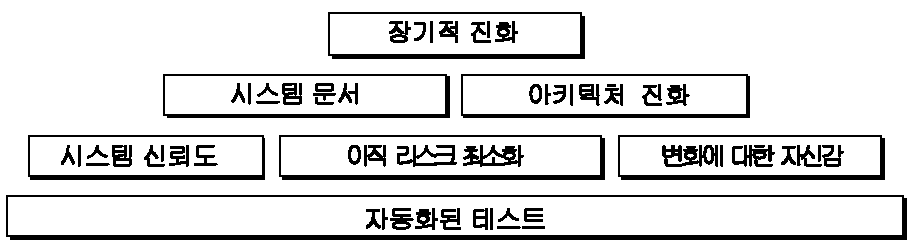
\includegraphics[width=\textwidth]{TestingFoundation}
\caption{Automated tests are the \emph{foundation} for reengineering. They establish your confidence in the system, reduce risks, and improve confidence in your ability to change the system. }
\figlabel{TestingFoundation}
\end{center}
\end{figure}

\noindent
Tests represent confidence in a system, because they specify how parts of the system work in a \emph{verifiable} way, and because they can be run at any time to check if the system is still consistent. 

\index{Davis, Alan}
\begin{quotation}
\noindent
\emph{``... testing simply exposes the presence of flaws in a program; it cannot be used to verify the absence of flaws. It can increase your confidence that a program is correct''}

\hfill --- Alan Davis, Principle 111 \cite{Davi95a}
\end{quotation}

Systematic testing is heavily promoted by \ind{Extreme Programming} \cite{Beck00a} one of the basic techniques necessary to be able to adapt programs quickly to changing requirements. Changing legacy systems is risky business. Will the code still work after a change? How many unexpected side-effects will appear? Having a set of automated, repeatable tests helps to reduce this risk. 

\begin{bulletlist}
\item A set of running tests provides confidence in the system. (``Are you really sure this piece of code works?'' ``Yes, look, here I have the tests that prove it.'')
\item A set of running tests represents \emph{reproducible} and \emph{verifiable} information about your system, and is at all times in sync with the application. This in contrast to most of the written documentation, which is typically slightly outdated already the next day.
\item Writing tests increases productivity, because bugs are found much earlier in the development process.
\end{bulletlist}

\subsection*{Related Patterns}

\patref{Write Tests to Enable Evolution}{WriteTestsToEnableEvolution} is a prerequisite to \patpgref{Always Have a Running Version}{AlwaysHaveARunningVersion}. Only with a comprehensive test program in place can you \patpgref{Migrate Systems Incrementally}{MigrateSystemsIncrementally}. 

\patref{Grow Your Test Base Incrementally}{GrowYourTestBaseIncrementally} and \patref{Test the Interface, Not the Implementation}{TestTheInterfaceNotTheImplementation} introduce a way to incrementally build a test suite while a system is evolving. 

%=================================================================
%:PATTERN -- {Grow Your Test Base Incrementally}
\pattern{Grow Your Test Base Incrementally}{GrowYourTestBaseIncrementally}


\intent{Balance the costs and the benefits of tests by incrementally introducing just the tests you need at a given point in time.}

\subsection*{Problem}

When should you start to introduce tests? When can you stop?

\emph{This problem is difficult because:}

\begin{bulletlist}
\item In a reengineering project, you cannot afford to spend too much time for writing tests.
\item Legacy systems tend to be huge, so testing everything is impossible.
\item Legacy systems tend to be poorly-documented and poorly-understood.
\item The original developers may have left and the system maintainers may have only limited knowledge of the system's inner workings.
\end{bulletlist}

\emph{Yet, solving this problem is feasible because:}

\begin{bulletlist}
\item We know where the fragile parts or the parts that we would like to change are.
\item We could convince programmers that they can benefit from tests.
\end{bulletlist}

\subsection*{Solution}

Introduce tests incrementally for parts of the system you are working on.

\subsubsection*{Hints}

\begin{bulletlist}
\item Carefully assess your priorities and initially develop tests only for the most critical components. As you reengineer the system, introduce tests for the new features, parts of the legacy that may be affected, and any bugs you identify along the way. 
\item Keep a snapshot of the old system handy so you can later introduce tests that should run against both the original system and its new incarnation.
\item Focus on business values. Start to write tests for the parts of your system that have the most important artifacts. Try to \patref{Record Business Rules as Tests}{RecordBusinessRulesAsTests}.
\item If you have the history of bug fixes or problems, apply \patpgref{Test Old Bugs}{TestOldBugs} as a starting point.
\item If you have acceptable documentation and some original developers of the system at hand, consider applying \patpgref{Test Fuzzy Features}{TestFuzzyFeatures}.
\item Apply \patref{Test the Interface, Not the Implementation}{TestTheInterfaceNotTheImplementation}, start to test big abstractions and then refine tests if time allows. For example, if you have a pipeline architecture, start to write tests that ensure you that the output of the full pipeline is right given the right input. Then write tests for the individual pipeline components.
\item Black-box test parts (subsystems, classes, methods) that are likely to change their implementation in the future.
\index{black box testing}
\end{bulletlist}

\subsection*{Tradeoffs}

\subsubsection*{Pros}

\begin{bulletlist}
\item You save time by only developing the tests that you need.
\item You build up a base of the most critical tests as the project progresses.
\item You build confidence as you go along
\item You streamline future development and maintenance activities.
\end{bulletlist}

\subsubsection*{Cons}

\begin{bulletlist}
\item You may guess wrong which aspects are critical to test.
\item Tests can give you false confidence --- untested bugs can still lurk in the system.
\end{bulletlist}

\subsubsection*{Difficulties}

\begin{bulletlist}
\item Setting-up the proper context for the tests may require considerable time and effort.
\item Identifying the boundaries of the components to test is just hard. Deciding which parts to test and how fine-grained these tests should be, requires a good understanding of the system and the way you intend to reengineer it.
\end{bulletlist}

\subsection*{Example}

\begin{figure}[h]
\begin{center}
\includegraphics[width=0.8\textwidth]{TestingChange}
\caption{Introduce tests for the parts of the system you intend to change.}
\figlabel{TestingChange}
\end{center}
\end{figure}

Initially introduce tests only for the subsystems and component you intend to change. In \figref{TestingChange} we introduce some tests for subsystem ABC and for its component B. We apply \patref{Test the Interface, Not the Implementation}{TestTheInterfaceNotTheImplementation} to ensure that the tests for B should also pass for newB.

Note that if we only introduce tests for component B, then we fail to test its integration with A and C. In any case, it may be that we fail to test all important aspects, so it is important to incrementally add new tests as bugs are detected and repaired.

\subsection*{Rationale}

An incremental testing strategy allows you to start reengineering efforts before all the tests are in place. By focussing on just those tests that concern the parts of the system you are currently changing, you enable change with a minimal investment in testing, while help your team build confidence as you grow your tests base.

\subsection*{Related Patterns}

\patref{Use a Testing Framework}{UseATestingFramework} to organize your tests. 

\patref{Test the Interface, Not the Implementation}{TestTheInterfaceNotTheImplementation} provides a strategy for developing tests at arbitrary granularities. \patref{Record Business Rules as Tests}{RecordBusinessRulesAsTests} provides another strategy for testing components that implement business logic. \patref{Write Tests to Understand}{WriteTestsToUnderstand} helps you prime a test base while you are still reverse engineering the system.

%=================================================================
%:PATTERN -- {Use a Testing Framework}
\pattern{Use a Testing Framework}{UseATestingFramework}

\intent{Encourage developers to write and use regression tests by providing a framework that makes it easy to develop, organize and run tests.}

\subsection*{Problem}

How do you encourage your team to adopt systematic testing?

\emph{This problem is difficult because:} 

\begin{bulletlist}
\item Tests are boring to write.
\item Tests may require a considerable test data to be built up and torn down.
\item It may be hard to distinguish between test failures and unexpected errors.
\end{bulletlist}

\emph{Yet, solving this problem is feasible because:}

\begin{bulletlist}
\item Most tests follow the same basic pattern: create some test data, perform some actions, see if the results match your expectations, clean up the test data.
\item Very little infrastructure is needed to run tests and report failures and errors.
\end{bulletlist}

\subsection*{Solution}

Use a testing framework that allows suites of tests to be composed from individual test cases.

\subsubsection*{Steps}

Unit testing frameworks, like \ind{JUnit} and \ind{SUnit} \cite{Beck98a}, and various commercial test harness packages are available for most programming languages. If a suitable testing framework is not available for the programming language you are using, you can easily brew your own according to the following principles:

\begin{bulletlist}
\item The user must provide test cases that set up test data, exercise them, and make assertions about the results
\item The testing framework should wrap test cases as tests which can distinguish between assertion failures and unexpected errors.
\item The framework should provide only minimal feedback if tests succeed.

\begin{bulletlist}
\item Assertion failures should indicate precisely which test failed.

\item Errors should result in more detailed feedback (such as a full stack trace).
\end{bulletlist}

\item The framework should allow tests to be composed as test suites.
\end{bulletlist}

\subsection*{Tradeoffs}

\subsubsection*{Pros}

\begin{bulletlist}
\item A testing framework simplifies the formulation of tests and encourages programmers to write tests and use them.
\end{bulletlist}

\subsubsection*{Cons}

\begin{bulletlist}
\item Testing requires commitment, discipline and support. You must convince your team of the need and benefits of disciplined testing, and you must integrate testing into your daily process. One way of supporting this discipline is to have one testing coach in your team; consider this when you \patpgref{Appoint a Navigator}{AppointANavigator}.
\end{bulletlist}

\subsection*{Example}

\begin{figure}[tb]
\begin{center}
\includegraphics[width=\textwidth]{TestingJUnit}
\caption{JUnit is a popular testing framework for Java that offers much more flexibility than the minimal scheme described above.}
\figlabel{TestingJUnit}
\end{center}
\end{figure}

\ind{JUnit} is a popular testing framework for Java, which considerable enhances the basic scheme described above. \figref{TestingJUnit} shows that the framework requires users to define their tests as subclasses of \lct{TestCase}. Users must provide the methods \lct{setUp()}, \lct{runTest()} and \lct{tearDown()}. The default implementation of \lct{setup()} and \lct{tearDown()} are empty, and the default implementation of \lct{runTest()} looks for and runs a method which is the name of the test (given in the constructor). These user-supplied hook methods are then called by the \lct{runBare()} template method.

JUnit manages the reporting of failures and errors with the help of an additional \lct{TestResult} class. In the design of JUnit, it is an instance of \lct{TestResult} that actually runs the tests and logs errors or failures. In \figref{TestingTestrun} we see a scenario in which a \lct{TestCase}, in its run method, passes control to an instance of \lct{TestResult}, which in turn calls the \lct{runBare} template method of the \lct{TestCase}.

\begin{figure}[tb]
\begin{center}
\includegraphics[width=\textwidth]{TestingTestrun}
\caption{In JUnit, tests are actually run by an instance of \lct{TestResult}, which invokes the \lct{runBare} template method of a \lct{TestCase}. The user only needs to provide the \lct{setUp()} and \lct{tearDown()} methods, and the test method to be invoked by \lct{runTest()}.}
\figlabel{TestingTestrun}
\end{center}
\end{figure}

\lct{TestCase} additionally provides a set of different kinds of standard assertion methods, such as \lct{assertEquals}, \lct{assertFails}, and so on. Each of these methods throws an \lct{AssertionFailedError}, which can be distinguished from any other kind of exception.

In order to use the framework, we will typically define a new class, say \lct{TestHashtable}, that bundles a set of test suites for a given class, \lct{Hashtable}, that we would like to test. The test class should extend \lct{junit.framework.TestCase}:

\begin{code}
import junit.framework.*;
import java.util.Hashtable;

public class TestHashtable extends TestCase {
\end{code}

The instance variables of the test class will hold the fixture - the actual test data:

\begin{code}
	private Hashtable boss;
	private String joe = "Joe";
	private String mary = "Mary";
	private String dave = "Dave";
	private String boris = "Boris";
\end{code}

There should be constructor that takes the name of a test case as its parameter. Its behavior is defined by its superclass:

\begin{code}
	public TestHashtable(String name) {
		super(name);
	}
\end{code}

The \lct{setUp()} \ind{hook method} can be overridden to set up the fixture. If there is any cleanup activity to be performed, we should also override \lct{tearDown()}. Their default implementations are empty.

\begin{code}
	protected void setUp() {
		boss = new Hashtable();
	}
\end{code}

We can then define any number of test cases that make use of the fixture. Note that each test case is independent, and will have a fresh copy of the fixture. (In principle, we should design tests that not only exercise the entire interface, but the test data should cover both typical and boundary cases. The sample tests shown here are far from complete.) 

Each test case should start with the characters ``test":

\begin{code}
	public void testEmpty() {
		assert(boss.isEmpty());
		assertEquals(boss.size(), 0);
		assert(!boss.contains(joe));
		assert(!boss.containsKey(joe));
	}

	public void testBasics() {
		boss.put(joe, mary);
		boss.put(mary, dave);
		boss.put(boris, dave);
		assert(!boss.isEmpty());
		assertEquals(boss.size(), 3);
		assert(boss.contains(mary));
		assert(!boss.contains(joe));
		assert(boss.containsKey(mary));
		assert(!boss.containsKey(dave));
		assertEquals(boss.get(joe), mary);
		assertEquals(boss.get(mary), dave);
		assertEquals(boss.get(dave), null);
	}
\end{code}

You may provide a static method \lct{suite()} which will build an instance of \lct{junit.framework.TestSuite} from the test cases defined by this class:

\begin{code}
	public static TestSuite suite() {
		TestSuite suite = new TestSuite();
		suite.addTest(new TestHashtable("testBasics"));
		suite.addTest(new TestHashtable("testEmpty"));
		return suite;
	}
}
\end{code}

The test case class should be compiled, together with any class it depends on.

\begin{figure}
\begin{center}
\includegraphics[width=0.8\textwidth]{TestingTestRunner}
\caption{An instance of \lct{java.ui.TestRunner}.}
\figlabel{TestingTestRunner}
\end{center}
\end{figure}

To run the tests, we can start up any one of a number of \emph{test runner} classes provided by the JUnit framework, for instance \lct{junit.ui.TestRunner} (see \figref{TestingTestRunner}).

\begin{figure}
\begin{center}
\includegraphics[width=0.8\textwidth]{TestingSuccess}
\caption{A successful test run.}
\figlabel{TestingSuccess}
\end{center}
\end{figure}

This particular test runner expects you to type in the name of the test class. You may then \emph{run} the tests defined by this class. The test runner will look for the suite method and use it to build an instance of \lct{TestSuite}. If you do not provide a static \lct{suite} method, the test runner will automatically build a test suite assuming that all the methods named test* are test cases. The test runner then runs the resulting test suite. The interface will report how many tests succeeded (see \figref{TestingSuccess}). A successful test run will show a green display. If any individual test fails, the display will be red, and details of the test case leading to the failure will be given.

\subsection*{Rationale}

A testing framework makes it easier to organize and run tests. 

Hierarchically organizing tests makes it easier to run just the tests that concern the part of the system you are working on.

\subsection*{Known Uses}

Testing frameworks exist for a vast number of languages, including Ada, ANT, C, C++, Delphi, .Net (all languages), Eiffel, Forte 4GL, GemStone/S, Jade, JUnit Java, JavaScript, k language (ksql, from kbd), Objective C, Open Road (CA), Oracle, PalmUnit, Perl, PhpUnit, PowerBuilder, Python, Rebol, `Ruby, Smalltalk, Visual Objects and UVisual Basic.

Beck and Gamma give a good overview in the context of JUnit \cite{Beck98a}.

%=================================================================
%:PATTERN -- {Test the Interface, Not the Implementation}
\pattern{Test the Interface, Not the Implementation}{TestTheInterfaceNotTheImplementation}

\emph{Also Known As:}  Black-Box Testing \cite{Pres94a}

\intent{Build up reusable tests that focus on external behavior rather than on implementation details, and thereby will survive changes to the system.}

\subsection*{Problem}

How can you develop tests that not only protect your software legacy, but also will continue to be valuable as the system changes?

\emph{This problem is difficult because:}

\begin{bulletlist}
\item Legacy systems have many features that should continue to function as the system evolves.
\item You cannot afford to spend too much time writing tests while reengineering the system.
\item You do not want to waste effort in developing tests that will have to be changed as you change the system.
\end{bulletlist}

\emph{Yet, solving this problem is feasible because:}

\begin{bulletlist}
\item The interfaces to the components of the system tell you what should be tested.
\item Interfaces tend to be more stable than implementations
\end{bulletlist}

\subsection*{Solution}

Develop black-box tests that exercise the public interface of your components.

\subsubsection*{Hints}

\begin{bulletlist}
\item Be sure to exercise boundary values (\ie minimum and maximum values for method parameters). The most common errors occur here.
\item Use a top-down strategy to develop black-box tests if there are many fine-grained components that you do not initially have time to develop tests for.
\item Use a bottom-up strategy if you are replacing functionality in a very focussed part of the legacy system.
\end{bulletlist}

\subsection*{Tradeoffs}

\subsubsection*{Pros}

\begin{bulletlist}
\item Tests that exercise public interfaces are more likely to be reusable if the implementation changes.
\item Black-box tests can often be used to exercise multiple implementations of the same interface.
\item It is relatively easy to develop tests based on a component's interface.
\item Focusing on the external behavior reduces considerably the possible tests to be written while still covering the essential aspects of a system.
\end{bulletlist}

\subsubsection*{Cons}

\begin{bulletlist}
\item Back-box tests will not necessarily exercise all possible program paths. You may have to use a separate coverage tool to check whether your tests cover all the code.
\item If the interface to a component changes you will still have to adapt the tests.
\end{bulletlist}

\subsubsection*{Difficulties}

\begin{bulletlist}
\item Sometimes the class does not provide the right interface to support black-box testing. Adding accessors to sample the state of the object can be a simple solution, but this generally weakens encapsulation and makes the object less of a black box.
\end{bulletlist}

\subsection*{Example}

Let's look back at the test presented in \patref{Write Tests to Enable Evolution}{WriteTestsToEnableEvolution}. The code we saw earlier was supposed to check whether the add operation defined on a class \lct{Money} works as expected. However, we see that the assert in line (3) actually depends on the internal implementation of the \lct{Money} class, because it checks for equality by accessing the parts of equality.

\begin{code}
public class MoneyTest extends TestCase {
	// ...
		public void testSimpleAdd() {
			Money m12CHF= new Money(12, "CHF");                 // (1)
			Money m14CHF= new Money(14, "CHF");        
			Money expected= new Money(26, "CHF");
			Money result= m12CHF.add(m14CHF);                      // (2)
			assert(result.currency().equals(expected.currency())
				&& result.amount() == expected.amount());            // (3)
		}
}
\end{code}

However, if the class \lct{Money} would override the default \lct{equals} operation defined on \lct{Object} (doing so would also require us to override \lct{hashCode}), the last assert statement could be simplified and would become independent of the internal implementation.

\begin{code}
public class MoneyTest extends TestCase {
	// ...
		public void testSimpleAdd() {
			Money m12CHF= new Money(12, "CHF");            // (1)
			Money m14CHF= new Money(14, "CHF");        
			Money expected= new Money(26, "CHF");
			Money result= m12CHF.add(m14CHF);                // (2)
			assert(expected.equals(result));                            // (3)
		}
}
\end{code}

\subsection*{Rationale}

The interface of a component is a direct consequence of its collaborations with other components. Black-box tests therefore have a good chance of exercising the most important interactions of a system.

Since interfaces tend to be more stable than implementations, black-box tests have a good chance of surviving major changes to the system, and they thereby protect your investment in developing tests.

\subsection*{Known Uses}

Black-Box testing is a standard testing strategy \cite{Somm96a}.

\subsection*{Related Patterns}

\patref{Record Business Rules as Tests}{RecordBusinessRulesAsTests} adopts a different strategy to developing tests which focuses on exercising business rules. This is fine if the components to be tested are the ones that implement the business logic. For most other components, \patref{Test the Interface, Not the Implementation}{TestTheInterfaceNotTheImplementation} will likely be more appropriate.

\index{black box testing}
\index{white box testing}
Components that implement complex algorithms may not be well-suited to black-box testing, since an analysis of the interface alone may not reveal all the cases that the algorithm should handle. White-box testing \cite{Somm96a} is another standard technique for testing algorithms in which test cases are generated to cover all possible paths through an algorithm.

%=================================================================
%:PATTERN -- {Record Business Rules as Tests}
\pattern{Record Business Rules as Tests}{RecordBusinessRulesAsTests}


\intent{Keep the system in sync with the business rules it implements by encoding the rules explicitly as tests.}

\subsection*{Problem}

How do you keep the \emph{actual business rules}, the \emph{documentation} about those business rules and the system \emph{implementation} in sync, while all three are changing?

\emph{This problem is difficult because:}

\begin{bulletlist}
\item Written documentation gets out of date quickly and does not ensure you that your system really implements the description of the business rules you have.
\item Business rules tend to be implicit in the code. It may not be obvious which pieces of software are responsible for computing a given business rule.
\item Developer turn-over introduces a high risk for your business by having more and more people knowing less and less about the system.
\item Most of the time only one programmer or user knows specific rules, and that person could be leaving tomorrow.
\item Business rules are likely to change due to external factors, such as the introduction of a new law, so it is important to represent them explicitly.
\end{bulletlist}

\emph{Yet, solving this problem is feasible because:}

\begin{bulletlist}
\item Most business rules are well expressed by sets of canonical examples, each of which requires certain well-defined actions to be taken, and results in some clear, observable results.
\end{bulletlist}

\subsection*{Solution}

Write executable tests that record the business rules as test cases, actions, and tests over the results. When tests break, you know that things are out of sync.

\subsubsection*{Hints}

\begin{bulletlist}
\item Developers and clients can write tests. Developers may write tests associated with specific functionality or piece of code. User may also have to write integration tests in the form of use cases that bind together several unit tests \cite{Davi95a} \cite{Beck00a}. 
\item Note that you are not interested in the implementation strategies or optimization aspects, but only the business rules. 
\end{bulletlist}

\subsection*{Tradeoffs}

\subsubsection*{Pros}

\begin{bulletlist}
\item The rules become explicit, thereby reducing dependency on human memory.
\item You need to record the business rules anyway before you can reengineer the legacy system.
\item Recording business rules as tests enables evolution: when new features must be added, you can check that the existing business rules are still correctly implemented by running the regression tests. On the other hand, when the business rules change, you can update the corresponding tests to reflect the changes.
\end{bulletlist}

\subsubsection*{Cons}

\begin{bulletlist}
\item Tests can only encode concrete scenarios, not actual the logic of the business rules themselves.
\item When the business logic must deal with an extremely large number of cases, it may be impractical to test them all.
\end{bulletlist}

\subsubsection*{Difficulties}

\begin{bulletlist}
\item Recording business rules does not mean extracting them. Extracting business rules from code with the current technology is a pipe dream.
\item Recording business rules can be difficult for system whose original developers and users have all left. 
\end{bulletlist}

\subsection*{Examples}

In this example we compute the amount of additional money an employee receives for a child. The rule states that a person or couple gets an amount of money for every child he, she or they raise. Basically parents get CHF 150,- per month for every child younger than 12 years, and CHF 180,- for every child between 12 and 18 and for every child between 18 and 25 as long as the child is not working and is still in the educational system. A single parent gets the full 100\% of this money as long as he or she is working more than 50\%. Couples get a percentage of the money that is equal to the summed working percentages of both partners.

The following \ind{Smalltalk} code shows a test that hardcodes the expected outcomes for the different computations. It allows for automatically checking the outcomes instead of having to print the outcomes and check by hand if they are right, and it acts as a regression test. Secondly it documents the expected outcome of the different computations.

\begin{code}
testMoneyGivenForKids
	|	singlePerson80occupationWithOneKidOf5
		couplePerson40occupationWithOneKidOf5
		couplePerson100occupationWith2KsidOf5
		couplePersonWithOneKidOf14 |

"cases are extracted from a database after the system has
performed the computation"

singlePerson80WithOneKidOf5 := extract....
couplePerson40occupationWithOneKidOf5 := extract....
couplePerson100occupationWithOneKidOf5 := extract....
couplePersonWithOneKidOf14 := extract....
"tests"

"We test that the right amount of money is computed correctly"

self assert: singlePerson80occupationWithOneKidOf5 moneyForKid = 150.
self assert: couplePerson40occupationWithOneKidOf5 moneyForKid = 150*4.
self assert: couplePerson100occupationWith2KidsOf5 moneyForKid = 150*2.
self assert: couplePersonWithOneKidOf14 moneyForKid = 180.
\end{code}

\subsection*{Rationale}

Tests are a good way to document what the system does. By documenting business rules as tests, you guarantee that the description of the business rules will be in sync with the implementation. 

The beginning of a reengineering project is a good point in time to set up a process to document knowledge about the system as explicit tests.

\subsection*{Related Patterns}

While you are reverse engineering a legacy system, you may \patref{Write Tests to Understand}{WriteTestsToUnderstand}. During this process it will be natural to \patref{Record Business Rules as Tests}{RecordBusinessRulesAsTests}. In this way you can prime your test base as you \patref{Grow Your Test Base Incrementally}{GrowYourTestBaseIncrementally}.

%=================================================================
%:PATTERN -- {Write Tests to Understand}
\pattern{Write Tests to Understand}{WriteTestsToUnderstand}

\intent{Record your understanding of a piece of code in the form of executable tests, thus setting the stage for future changes.}

\subsection*{Problem}

How do you develop an understanding of a part of a legacy system which contains neither tests nor accurate and precise documentation?

\emph{This problem is difficult because:}

\begin{bulletlist}
\item Code is always difficult to understand.
\item You would like to make hypotheses about what the code is really doing and validate them.
\item You would like to specify as precisely as possible the behavior of the system.
\item You would like to record your understanding to communicate it but you do not want to waste your time in writing documents that will be obsolete as soon as you start changing the code. 
\end{bulletlist}

\emph{Yet, solving this problem is feasible because:}

\begin{bulletlist}
\item The piece of code is relatively small and has clearly defined boundaries.
\item You have the possibility to specify tests and validate them.
\end{bulletlist}

\subsection*{Solution}

Encode your hypotheses and conclusions as executable tests.

\subsection*{Tradeoffs}

\subsubsection*{Pros}

\begin{bulletlist}
\item Tests help you to validate your understanding.
\item Tests can provide a precise specification of certain aspects of the system. Tests cannot be fuzzy.
\item Tests can be applied to gain different levels of understanding. For example, black-box tests can help you to refine your understanding of roles and collaborations, whereas white-box tests can help you to gain understanding of the implementation of complex logic.
\item The tests that you develop will help to enable future reengineering effort.
\item Tests will force you to be precise about the creation and the use of the objects under test.
\end{bulletlist}

\subsubsection*{Cons}

\begin{bulletlist}
\item Writing tests is time consuming.
\end{bulletlist}

\subsubsection*{Difficulties}

\begin{bulletlist}
\item Obtaining a well defined context in which you can test the objects is difficult especially if the objects to be tested do not represent specific abstractions. Looking for the places where objects you want to understand are created can help. 
\item Concurrent systems are known to be difficult to test, so tests can miss important aspects (such as handling of race conditions).
\end{bulletlist}

\subsection*{Rationale}

By writing automated tests, you exercise parts of the system you want to understand, while recording your understanding and setting the stage for future reengineering effort.

\subsection*{Related Patterns}

Before writing any tests, you might want to \patpgref{Refactor to Understand}{RefactorToUnderstand}. As you write your tests, be sure to \patpgref{Tie Code and Questions}{TieCodeAndQuestions}.

%=============================================================
\ifx\wholebook\relax\else
   \bibliographystyle{alpha}
   \bibliography{scg}
   \end{document}
\fi
%=============================================================

% $Author: oscar $
% $Date: 2009-09-15 16:53:48 +0200 (Tue, 15 Sep 2009) $
% $Revision: 29111 $
%=================================================================
\ifx\wholebook\relax\else
% --------------------------------------------
% Lulu:
	\documentclass[a4paper,10pt,twoside]{book}
	\usepackage[
		papersize={6.13in,9.21in},
		hmargin={.815in,.815in},
		vmargin={.98in,.98in},
		ignoreheadfoot
	]{geometry}
	\usepackage[hangul]{kotex}
	% $Author: oscar $
% $Date: 2009-09-13 20:58:29 +0200 (Sun, 13 Sep 2009) $
% $Revision: 29070 $
%=============================================================
% NB: documentclass must be set in main document.
% Allows book to be generated in multiple formats.
%=============================================================
%:Packages
\usepackage[T1]{fontenc}  %%%%%really important to get the code directly in the text!
\usepackage{palatino}
\usepackage{ifthen}
\usepackage{graphicx}
\graphicspath{{figures/}}
\usepackage{xspace}
\usepackage{makeidx}
\usepackage{isodateo} % enable \isodate
\usepackage{amssymb,textcomp}
%=============================================================
%:More packages
%\usepackage[english]{babel}
%\usepackage{lmodern}
%\usepackage[scaled=0.85]{helvet}
%\usepackage{microtype}
%\usepackage{theorem}
%\usepackage{float}
%\usepackage{longtable}
%\usepackage[nottoc]{tocbibind}
%\usepackage{multicol}
%\usepackage{booktabs}	% book-style tables
%\usepackage{topcapt}	% enables \topcaption
%\usepackage{multirow}
%\usepackage{tabularx}
%\usepackage{alltt}
\usepackage[usenames,dvipsnames]{color}
%\usepackage[hang]{subfigure}\makeatletter\def\p@subfigure{\thefigure\,}\makeatother
%\usepackage{rotating}
%\usepackage{enumitem}	% apb: allows more control over tags in enumerations
%\usepackage{verbatim}     % for comment environment
%\usepackage{varioref}	% for page references that work
%\usepackage{needspace}
%\usepackage[newparttoc]{titlesec}
%\usepackage{titletoc}
%\usepackage{wrapfig}
\usepackage[
	colorlinks=true,
	linkcolor=black,
	urlcolor=black,
	citecolor=black
]{hyperref}   % should come last
%=============================================================
%:URL style
\makeatletter
\def\url@leostyle{%
  \@ifundefined{selectfont}{\def\UrlFont{\sf}}{\def\UrlFont{\sffamily}}}
\makeatother
\urlstyle{leo}
%=============================================================
%:Booleans
\newboolean{lulu}
\setboolean{lulu}{false}
\newcommand{\ifluluelse}[2]{\ifthenelse{\boolean{lulu}}{#1}{#2}}
%=============================================================
%:Editorial comment macros
\newcommand{\nnbb}[2]{
  \fbox{\bfseries\sffamily\scriptsize#1}
  {\sf\small$\blacktriangleright$\textit{#2}$\blacktriangleleft$}
}
\newcommand{\on}[1]{\nnbb{Oscar}{#1}}
\newcommand{\here}{\nnbb{CONTINUE}{HERE}}
%=============================================================
%:Abbreviation macros
\newcommand{\ie}{\emph{i.e.},\xspace}
\newcommand{\eg}{\emph{e.g.},\xspace}
\newcommand{\etc}{\emph{etc.}\xspace}
\newcommand{\etal}{\emph{et al.}\xspace}
\newcommand{\straightquote}{"}
\newcommand{\sba}{\url{SquareBracketAssociates.org}\xspace}
%=============================================================
%:Patterns
% \newcommand{\pattern}[2]{\newpage\section{{\sf #1}}\label{pat:#2}}
% \newcommand{\pattern}[2]{\newpage\index{#1 (Pattern)}\section{#1}\label{pat:#2}}
\newcommand{\pattern}[2]{\cleardoublepage\index{#1 (패턴)}\section{#1}\label{pat:#2}}
\newcommand{\thumbnail}[2]{\index{#1 (패턴)}\subsection{#1}\label{pat:#2}}
\newcommand{\thumblang}[2]{\index{#1 (패턴 랭귀지)}\subsection{#1}\label{pat:#2}}
\newcommand{\variant}[1]{{\emph{#1}}\xspace}
% \newcommand{\problem}[1]{\subsection*{Problem}\emph{#1}}
\newcommand{\intent}[1]{\paragraph{의도}\emph{#1}}
\newcommand{\problem}[1]{\paragraph{문제}\emph{#1}}
\newcommand{\solution}[1]{\paragraph{해결}\emph{#1}}
\newcommand{\discussion}[0]{\paragraph{토론}}
\newcommand{\cmd}[1]{{\tt #1}\xspace}
%=============================================================
%:Environments
\newenvironment{bulletlist}{\begin{itemize}\setlength{\itemsep}{0ex}}
{\end{itemize}}
%=============================================================
%:Cross reference macros
\newcommand{\chalabel}[1]{\label{cha:#1}}
\newcommand{\seclabel}[1]{\label{sec:#1}}
\newcommand{\figlabel}[1]{\label{fig:#1}}
\newcommand{\tablabel}[1]{\label{tab:#1}}
\newcommand{\rulelabel}[1]{\label{rule:#1}}
\newcommand{\eglabel}[1]{\label{eg:#1}}
\newcommand{\scrlabel}[1]{\label{scr:#1}}
\newcommand{\mthlabel}[1]{\label{mth:#1}}
\newcommand{\clslabel}[1]{\label{cls:#1}}
\newcommand{\faqlabel}[1]{\label{faq:#1}}
%\newcommand{\charef}[1]{Chapter~\ref{cha:#1}\xspace}
%\newcommand{\secref}[1]{Section~\ref{sec:#1}\xspace}
\newcommand{\figref}[1]{Figure~\ref{fig:#1}\xspace}
% \newcommand{\patpgref}[2]{\hyperref[pat:#2]{\sf #1} [p.~\pageref{pat:#2}]\xspace}
\newcommand{\patpgref}[2]{\index{#1 (Pattern)}\hyperref[pat:#2]{#1} [p.~\pageref{pat:#2}]\xspace}
\newcommand{\patlangpgref}[2]{\index{#1 (Pattern language)}\hyperref[pat:#2]{#1} [p.~\pageref{pat:#2}]\xspace}
% \newcommand{\patref}[2]{\hyperref[pat:#2]{\sf #1}\xspace}
\newcommand{\patref}[2]{\index{#1 (Pattern)}\hyperref[pat:#2]{#1}\xspace}
\newcommand{\patlangref}[2]{\index{#1 (Pattern language)}\hyperref[pat:#2]{#1}\xspace}
% \newcommand{\charef}[2]{\hyperref[cha:#2]{\underline{\sf #1}}\xspace}
% \newcommand{\charef}[2]{\hyperref[cha:#2]{\sf #1}\xspace}
\newcommand{\charef}[2]{\index{#1 (Pattern cluster)}\hyperref[cha:#2]{#1}\xspace}
% \newcommand{\chapgref}[2]{\hyperref[cha:#2]{\sf #1} [p.~\pageref{cha:#2}]\xspace}
\newcommand{\chapgref}[2]{\index{#1 (Pattern cluster)}\hyperref[cha:#2]{#1} [p.~\pageref{cha:#2}]\xspace}
%\newcommand{\Figref}[1]{Figure~\ref{fig:#1}\xspace}
%\newcommand{\appref}[1]{Appendix~\ref{app:#1}\xspace}
%\newcommand{\tabref}[1]{Table~\ref{tab:#1}\xspace}
%\newcommand{\ruleref}[1]{\ref{rule:#1}\xspace}
%\newcommand{\egref}[1]{example~\ref{eg:#1}\xspace}
%\newcommand{\Egref}[1]{Example~\ref{eg:#1}\xspace}
%\newcommand{\scrref}[1]{script~\ref{scr:#1}\xspace}
%\newcommand{\Scrref}[1]{Script~\ref{scr:#1}\xspace}
%\newcommand{\tscrref}[1]{the script~\ref{scr:#1}\xspace}
%\newcommand{\Tscrref}[1]{The script~\ref{scr:#1}\xspace}
%\newcommand{\mthref}[1]{method~\ref{mth:#1}\xspace}
%\newcommand{\mthsref}[1]{methods~\ref{mth:#1}\xspace}
%\newcommand{\Mthref}[1]{Method~\ref{mth:#1}\xspace}
%\newcommand{\tmthref}[1]{the method~\ref{mth:#1}\xspace}
%\newcommand{\Tmthref}[1]{The method~\ref{mth:#1}\xspace}
%\newcommand{\clsref}[1]{class~\ref{cls:#1}\xspace}
%\newcommand{\tclsref}[1]{the class~\ref{cls:#1}\xspace}
%\newcommand{\Tclsref}[1]{The class~\ref{cls:#1}\xspace}
%=============================================================
%:Page Layout
\setlength{\headsep}{1cm}
%=============================================================
%:Menu item macro
%\definecolor{lightgray}{gray}{0.89}
%\newcommand{\menu}[1]{{%
%	\setlength{\fboxsep}{0pt}%
%	\colorbox{lightgray}{{{\upshape\sffamily\strut \,#1\,}}}}}
%\newcommand{\go}{\,$\triangleright$\,}
%\newcommand{\short}[1]{\mbox{{\sc cmd}\hspace{0.08em}--\hspace{0.09em}#1}\xspace}
%\newcommand{\button}[1]{{%
%	\setlength{\fboxsep}{0pt}%
%	\fbox{{\upshape\sffamily\strut \,#1\,}}}}
%\newcommand{\toolsflap}{\textit{Tools} flap\xspace}
%=============================================================
%:Section depth
%\setcounter{secnumdepth}{2}
%
%\DeclareGraphicsExtensions{.pdf, .jpg, .png}
%=============================================================
%:PDF setup
\hypersetup{
   pdftitle={Object-Oriented Reengineering Patterns},
   pdfauthor={Serge Demeyer, St\'ephane Ducasse, Oscar Nierstrasz},
   pdfkeywords={Reengineering, Object-Oriented Programming, Patterns},
   pdfsubject={Computer Science}
}
%=============================================================
%:Page layout and appearance
%\renewcommand{\chaptermark}[1]{\markboth{#1}{}}
%\renewcommand{\sectionmark}[1]{\markright{\thesection\ #1}}
%\renewpagestyle{plain}[\small\itshape]{%
%	\setheadrule{0pt}%
%	\sethead[][][]{}{}{}%
%	\setfoot[][][]{}{}{}}
%\renewpagestyle{headings}[\small\itshape]{%
%	\setheadrule{0pt}%
%	\setmarks{chapter}{section}%
%	\sethead[\thepage][][\chaptertitle]{\sectiontitle}{}{\thepage}%
%	\setfoot[][][]{}{}{}}
%=============================================================
%:Title section setup and TOC numbering depth
%\setcounter{secnumdepth}{1}
%\setcounter{tocdepth}{1}
%\titleformat{\part}[display]{\centering}{\huge\partname\ \thepart}{1em}{\Huge\textbf}[]
%\titleformat{\chapter}[display]{}{\huge\chaptertitlename\ \thechapter}{1em}{\Huge\raggedright\textbf}[]
%\titlecontents{part}[3pc]{%
%		\pagebreak[2]\addvspace{1em plus.4em minus.2em}%
%		\leavevmode\large\bfseries}
%	{\contentslabel{3pc}}{\hspace*{-3pc}}
%	{}[\nopagebreak]
%\titlecontents{chapter}[3pc]{%
%		\pagebreak[0]\addvspace{1em plus.2em minus.2em}%
%		\leavevmode\bfseries}
%	{\contentslabel{3pc}}{}
%	{\hfill\contentspage}[\nopagebreak]
%\dottedcontents{section}[3pc]{}{3pc}{1pc}
%\dottedcontents{subsection}[3pc]{}{0pc}{1pc}
%\let\origdoublepage\cleardoublepage
%\newcommand{\clearemptydoublepage}{%
%  \clearpage
%  {\pagestyle{empty}\origdoublepage}}
%\let\cleardoublepage\clearemptydoublepage % see http://www.tex.ac.uk/cgi-bin/texfaq2html?label=patch
%=============================================================
%:Listings package configuration
\newcommand{\caret}{\makebox{\raisebox{0.4ex}{\footnotesize{$\wedge$}}}}
% \newcommand{\escape}{{\sf \textbackslash}}
\definecolor{source}{gray}{0.95}
\usepackage{listings}
\lstdefinelanguage{Smalltalk}{
  morestring=[d]',
% Adapt this to other languages!
%  morecomment=[s]{"}{"},
  alsoletter={\#:},
  %escapechar={!},
  literate=
    {BANG}{!}1
%    {UNDERSCORE}{\_}1
    {\\st}{Smalltalk}9 % convenience -- in case \st occurs in code
    % {'}{{\textquotesingle}}1 % replaced by upquote=true in \lstset
%    {_}{{$\leftarrow$}}1
    {>>>}{{\sep}}1
    {^}{{$\uparrow$}}1
    {~}{{$\sim$}}1
    {-}{{\sf -\hspace{-0.13em}-}}1  % the goal is to make - the same width as +
    {+}{\raisebox{0.08ex}{+}}1		% and to raise + off the baseline to match -
    {-->}{{\quad$\longrightarrow$\quad}}3
	, % Don't forget the comma at the end!
  tabsize=4
}[keywords,comments,strings]

\lstset{language=Smalltalk,
	basicstyle=\sffamily,
	keywordstyle=\color{black}\bfseries,
	% stringstyle=\ttfamily, % Ugly! do we really want this? -- on
	mathescape=true,
	showstringspaces=false,
	keepspaces=true,
	breaklines=true,
	breakautoindent=true,
	backgroundcolor=\color{source},
	lineskip={-1pt}, % Ugly hack
	upquote=true, % straight quote; requires textcomp package
	columns=fullflexible} % no fixed width fonts
% \newcommand{\ct}{\lstinline[mathescape=false,basicstyle={\sffamily\upshape}]}
\newcommand{\ct}{\lstinline[mathescape=false,backgroundcolor=\color{white},basicstyle={\sffamily\upshape}]}
\newcommand{\lct}[1]{{\textsf{\textup{#1}}}}
%\newcommand{\scat}[1]{\emph{\textsf{#1}}\xspace}
%\newcommand{\prot}[1]{\emph{\textsf{#1}}\xspace}
% NB: No argument!
\lstnewenvironment{code}[0]{%
	\lstset{%
		% frame=lines,
		frame=single,
		framerule=0pt,
		mathescape=false
	}
}{}
%\def\ignoredollar#1{}
%=============================================================
%:Reserving space
%\newcommand{\needlines}[1]{\Needspace{#1\baselineskip}}
%=============================================================
%:Indexing macros
% Macros ending with "ind" generate text as well as an index entry
% Macros ending with "index" *only* generate an index entry
\newcommand{\ind}[1]{\index{#1}#1\xspace} % plain text
\newcommand{\subind}[2]{\index{#1!#2}#2\xspace} % show #2, subindex under #1
\newcommand{\emphind}[1]{\index{#1}\emph{#1}\xspace} % emph #1
\newcommand{\emphsubind}[2]{\index{#1!#2}\emph{#2}\xspace} % show emph #2, subindex under #1
\newcommand{\patind}[1]{\index{#1@#1 (pattern)}\ct{#1}\xspace} % pattern
\newcommand{\seeindex}[2]{\index{#1|see{#2}}} % #1, see #2
%\newcommand{\boldidx}[1]{{\bf #1}} % breaks hyperlink
%\newcommand{\indmain}[1]{\index{#1}#1\xspace} 
%\newcommand{\emphsubindmain}[2]{\index{#1!#2}\emph{#2}\xspace} % subindex, main entry
%\newcommand{\subindmain}[2]{\index{#1!#2}#2\xspace} % subindex, main entry
%\newcommand{\clsindmain}[1]{\index{#1!\#@(class)}\ct{#1}\xspace} % class main
%\newcommand{\indexmain}[1]{\index{#1}} 
%=============================================================
\parskip 1ex
%=============================================================

	\pagestyle{headings}
	\setboolean{lulu}{true}
% --------------------------------------------
% A4:
%	\documentclass[a4paper,11pt,twoside]{book}
%	% $Author: oscar $
% $Date: 2009-09-13 20:58:29 +0200 (Sun, 13 Sep 2009) $
% $Revision: 29070 $
%=============================================================
% NB: documentclass must be set in main document.
% Allows book to be generated in multiple formats.
%=============================================================
%:Packages
\usepackage[T1]{fontenc}  %%%%%really important to get the code directly in the text!
\usepackage{palatino}
\usepackage{ifthen}
\usepackage{graphicx}
\graphicspath{{figures/}}
\usepackage{xspace}
\usepackage{makeidx}
\usepackage{isodateo} % enable \isodate
\usepackage{amssymb,textcomp}
%=============================================================
%:More packages
%\usepackage[english]{babel}
%\usepackage{lmodern}
%\usepackage[scaled=0.85]{helvet}
%\usepackage{microtype}
%\usepackage{theorem}
%\usepackage{float}
%\usepackage{longtable}
%\usepackage[nottoc]{tocbibind}
%\usepackage{multicol}
%\usepackage{booktabs}	% book-style tables
%\usepackage{topcapt}	% enables \topcaption
%\usepackage{multirow}
%\usepackage{tabularx}
%\usepackage{alltt}
\usepackage[usenames,dvipsnames]{color}
%\usepackage[hang]{subfigure}\makeatletter\def\p@subfigure{\thefigure\,}\makeatother
%\usepackage{rotating}
%\usepackage{enumitem}	% apb: allows more control over tags in enumerations
%\usepackage{verbatim}     % for comment environment
%\usepackage{varioref}	% for page references that work
%\usepackage{needspace}
%\usepackage[newparttoc]{titlesec}
%\usepackage{titletoc}
%\usepackage{wrapfig}
\usepackage[
	colorlinks=true,
	linkcolor=black,
	urlcolor=black,
	citecolor=black
]{hyperref}   % should come last
%=============================================================
%:URL style
\makeatletter
\def\url@leostyle{%
  \@ifundefined{selectfont}{\def\UrlFont{\sf}}{\def\UrlFont{\sffamily}}}
\makeatother
\urlstyle{leo}
%=============================================================
%:Booleans
\newboolean{lulu}
\setboolean{lulu}{false}
\newcommand{\ifluluelse}[2]{\ifthenelse{\boolean{lulu}}{#1}{#2}}
%=============================================================
%:Editorial comment macros
\newcommand{\nnbb}[2]{
  \fbox{\bfseries\sffamily\scriptsize#1}
  {\sf\small$\blacktriangleright$\textit{#2}$\blacktriangleleft$}
}
\newcommand{\on}[1]{\nnbb{Oscar}{#1}}
\newcommand{\here}{\nnbb{CONTINUE}{HERE}}
%=============================================================
%:Abbreviation macros
\newcommand{\ie}{\emph{i.e.},\xspace}
\newcommand{\eg}{\emph{e.g.},\xspace}
\newcommand{\etc}{\emph{etc.}\xspace}
\newcommand{\etal}{\emph{et al.}\xspace}
\newcommand{\straightquote}{"}
\newcommand{\sba}{\url{SquareBracketAssociates.org}\xspace}
%=============================================================
%:Patterns
% \newcommand{\pattern}[2]{\newpage\section{{\sf #1}}\label{pat:#2}}
% \newcommand{\pattern}[2]{\newpage\index{#1 (Pattern)}\section{#1}\label{pat:#2}}
\newcommand{\pattern}[2]{\cleardoublepage\index{#1 (패턴)}\section{#1}\label{pat:#2}}
\newcommand{\thumbnail}[2]{\index{#1 (패턴)}\subsection{#1}\label{pat:#2}}
\newcommand{\thumblang}[2]{\index{#1 (패턴 랭귀지)}\subsection{#1}\label{pat:#2}}
\newcommand{\variant}[1]{{\emph{#1}}\xspace}
% \newcommand{\problem}[1]{\subsection*{Problem}\emph{#1}}
\newcommand{\intent}[1]{\paragraph{의도}\emph{#1}}
\newcommand{\problem}[1]{\paragraph{문제}\emph{#1}}
\newcommand{\solution}[1]{\paragraph{해결}\emph{#1}}
\newcommand{\discussion}[0]{\paragraph{토론}}
\newcommand{\cmd}[1]{{\tt #1}\xspace}
%=============================================================
%:Environments
\newenvironment{bulletlist}{\begin{itemize}\setlength{\itemsep}{0ex}}
{\end{itemize}}
%=============================================================
%:Cross reference macros
\newcommand{\chalabel}[1]{\label{cha:#1}}
\newcommand{\seclabel}[1]{\label{sec:#1}}
\newcommand{\figlabel}[1]{\label{fig:#1}}
\newcommand{\tablabel}[1]{\label{tab:#1}}
\newcommand{\rulelabel}[1]{\label{rule:#1}}
\newcommand{\eglabel}[1]{\label{eg:#1}}
\newcommand{\scrlabel}[1]{\label{scr:#1}}
\newcommand{\mthlabel}[1]{\label{mth:#1}}
\newcommand{\clslabel}[1]{\label{cls:#1}}
\newcommand{\faqlabel}[1]{\label{faq:#1}}
%\newcommand{\charef}[1]{Chapter~\ref{cha:#1}\xspace}
%\newcommand{\secref}[1]{Section~\ref{sec:#1}\xspace}
\newcommand{\figref}[1]{Figure~\ref{fig:#1}\xspace}
% \newcommand{\patpgref}[2]{\hyperref[pat:#2]{\sf #1} [p.~\pageref{pat:#2}]\xspace}
\newcommand{\patpgref}[2]{\index{#1 (Pattern)}\hyperref[pat:#2]{#1} [p.~\pageref{pat:#2}]\xspace}
\newcommand{\patlangpgref}[2]{\index{#1 (Pattern language)}\hyperref[pat:#2]{#1} [p.~\pageref{pat:#2}]\xspace}
% \newcommand{\patref}[2]{\hyperref[pat:#2]{\sf #1}\xspace}
\newcommand{\patref}[2]{\index{#1 (Pattern)}\hyperref[pat:#2]{#1}\xspace}
\newcommand{\patlangref}[2]{\index{#1 (Pattern language)}\hyperref[pat:#2]{#1}\xspace}
% \newcommand{\charef}[2]{\hyperref[cha:#2]{\underline{\sf #1}}\xspace}
% \newcommand{\charef}[2]{\hyperref[cha:#2]{\sf #1}\xspace}
\newcommand{\charef}[2]{\index{#1 (Pattern cluster)}\hyperref[cha:#2]{#1}\xspace}
% \newcommand{\chapgref}[2]{\hyperref[cha:#2]{\sf #1} [p.~\pageref{cha:#2}]\xspace}
\newcommand{\chapgref}[2]{\index{#1 (Pattern cluster)}\hyperref[cha:#2]{#1} [p.~\pageref{cha:#2}]\xspace}
%\newcommand{\Figref}[1]{Figure~\ref{fig:#1}\xspace}
%\newcommand{\appref}[1]{Appendix~\ref{app:#1}\xspace}
%\newcommand{\tabref}[1]{Table~\ref{tab:#1}\xspace}
%\newcommand{\ruleref}[1]{\ref{rule:#1}\xspace}
%\newcommand{\egref}[1]{example~\ref{eg:#1}\xspace}
%\newcommand{\Egref}[1]{Example~\ref{eg:#1}\xspace}
%\newcommand{\scrref}[1]{script~\ref{scr:#1}\xspace}
%\newcommand{\Scrref}[1]{Script~\ref{scr:#1}\xspace}
%\newcommand{\tscrref}[1]{the script~\ref{scr:#1}\xspace}
%\newcommand{\Tscrref}[1]{The script~\ref{scr:#1}\xspace}
%\newcommand{\mthref}[1]{method~\ref{mth:#1}\xspace}
%\newcommand{\mthsref}[1]{methods~\ref{mth:#1}\xspace}
%\newcommand{\Mthref}[1]{Method~\ref{mth:#1}\xspace}
%\newcommand{\tmthref}[1]{the method~\ref{mth:#1}\xspace}
%\newcommand{\Tmthref}[1]{The method~\ref{mth:#1}\xspace}
%\newcommand{\clsref}[1]{class~\ref{cls:#1}\xspace}
%\newcommand{\tclsref}[1]{the class~\ref{cls:#1}\xspace}
%\newcommand{\Tclsref}[1]{The class~\ref{cls:#1}\xspace}
%=============================================================
%:Page Layout
\setlength{\headsep}{1cm}
%=============================================================
%:Menu item macro
%\definecolor{lightgray}{gray}{0.89}
%\newcommand{\menu}[1]{{%
%	\setlength{\fboxsep}{0pt}%
%	\colorbox{lightgray}{{{\upshape\sffamily\strut \,#1\,}}}}}
%\newcommand{\go}{\,$\triangleright$\,}
%\newcommand{\short}[1]{\mbox{{\sc cmd}\hspace{0.08em}--\hspace{0.09em}#1}\xspace}
%\newcommand{\button}[1]{{%
%	\setlength{\fboxsep}{0pt}%
%	\fbox{{\upshape\sffamily\strut \,#1\,}}}}
%\newcommand{\toolsflap}{\textit{Tools} flap\xspace}
%=============================================================
%:Section depth
%\setcounter{secnumdepth}{2}
%
%\DeclareGraphicsExtensions{.pdf, .jpg, .png}
%=============================================================
%:PDF setup
\hypersetup{
   pdftitle={Object-Oriented Reengineering Patterns},
   pdfauthor={Serge Demeyer, St\'ephane Ducasse, Oscar Nierstrasz},
   pdfkeywords={Reengineering, Object-Oriented Programming, Patterns},
   pdfsubject={Computer Science}
}
%=============================================================
%:Page layout and appearance
%\renewcommand{\chaptermark}[1]{\markboth{#1}{}}
%\renewcommand{\sectionmark}[1]{\markright{\thesection\ #1}}
%\renewpagestyle{plain}[\small\itshape]{%
%	\setheadrule{0pt}%
%	\sethead[][][]{}{}{}%
%	\setfoot[][][]{}{}{}}
%\renewpagestyle{headings}[\small\itshape]{%
%	\setheadrule{0pt}%
%	\setmarks{chapter}{section}%
%	\sethead[\thepage][][\chaptertitle]{\sectiontitle}{}{\thepage}%
%	\setfoot[][][]{}{}{}}
%=============================================================
%:Title section setup and TOC numbering depth
%\setcounter{secnumdepth}{1}
%\setcounter{tocdepth}{1}
%\titleformat{\part}[display]{\centering}{\huge\partname\ \thepart}{1em}{\Huge\textbf}[]
%\titleformat{\chapter}[display]{}{\huge\chaptertitlename\ \thechapter}{1em}{\Huge\raggedright\textbf}[]
%\titlecontents{part}[3pc]{%
%		\pagebreak[2]\addvspace{1em plus.4em minus.2em}%
%		\leavevmode\large\bfseries}
%	{\contentslabel{3pc}}{\hspace*{-3pc}}
%	{}[\nopagebreak]
%\titlecontents{chapter}[3pc]{%
%		\pagebreak[0]\addvspace{1em plus.2em minus.2em}%
%		\leavevmode\bfseries}
%	{\contentslabel{3pc}}{}
%	{\hfill\contentspage}[\nopagebreak]
%\dottedcontents{section}[3pc]{}{3pc}{1pc}
%\dottedcontents{subsection}[3pc]{}{0pc}{1pc}
%\let\origdoublepage\cleardoublepage
%\newcommand{\clearemptydoublepage}{%
%  \clearpage
%  {\pagestyle{empty}\origdoublepage}}
%\let\cleardoublepage\clearemptydoublepage % see http://www.tex.ac.uk/cgi-bin/texfaq2html?label=patch
%=============================================================
%:Listings package configuration
\newcommand{\caret}{\makebox{\raisebox{0.4ex}{\footnotesize{$\wedge$}}}}
% \newcommand{\escape}{{\sf \textbackslash}}
\definecolor{source}{gray}{0.95}
\usepackage{listings}
\lstdefinelanguage{Smalltalk}{
  morestring=[d]',
% Adapt this to other languages!
%  morecomment=[s]{"}{"},
  alsoletter={\#:},
  %escapechar={!},
  literate=
    {BANG}{!}1
%    {UNDERSCORE}{\_}1
    {\\st}{Smalltalk}9 % convenience -- in case \st occurs in code
    % {'}{{\textquotesingle}}1 % replaced by upquote=true in \lstset
%    {_}{{$\leftarrow$}}1
    {>>>}{{\sep}}1
    {^}{{$\uparrow$}}1
    {~}{{$\sim$}}1
    {-}{{\sf -\hspace{-0.13em}-}}1  % the goal is to make - the same width as +
    {+}{\raisebox{0.08ex}{+}}1		% and to raise + off the baseline to match -
    {-->}{{\quad$\longrightarrow$\quad}}3
	, % Don't forget the comma at the end!
  tabsize=4
}[keywords,comments,strings]

\lstset{language=Smalltalk,
	basicstyle=\sffamily,
	keywordstyle=\color{black}\bfseries,
	% stringstyle=\ttfamily, % Ugly! do we really want this? -- on
	mathescape=true,
	showstringspaces=false,
	keepspaces=true,
	breaklines=true,
	breakautoindent=true,
	backgroundcolor=\color{source},
	lineskip={-1pt}, % Ugly hack
	upquote=true, % straight quote; requires textcomp package
	columns=fullflexible} % no fixed width fonts
% \newcommand{\ct}{\lstinline[mathescape=false,basicstyle={\sffamily\upshape}]}
\newcommand{\ct}{\lstinline[mathescape=false,backgroundcolor=\color{white},basicstyle={\sffamily\upshape}]}
\newcommand{\lct}[1]{{\textsf{\textup{#1}}}}
%\newcommand{\scat}[1]{\emph{\textsf{#1}}\xspace}
%\newcommand{\prot}[1]{\emph{\textsf{#1}}\xspace}
% NB: No argument!
\lstnewenvironment{code}[0]{%
	\lstset{%
		% frame=lines,
		frame=single,
		framerule=0pt,
		mathescape=false
	}
}{}
%\def\ignoredollar#1{}
%=============================================================
%:Reserving space
%\newcommand{\needlines}[1]{\Needspace{#1\baselineskip}}
%=============================================================
%:Indexing macros
% Macros ending with "ind" generate text as well as an index entry
% Macros ending with "index" *only* generate an index entry
\newcommand{\ind}[1]{\index{#1}#1\xspace} % plain text
\newcommand{\subind}[2]{\index{#1!#2}#2\xspace} % show #2, subindex under #1
\newcommand{\emphind}[1]{\index{#1}\emph{#1}\xspace} % emph #1
\newcommand{\emphsubind}[2]{\index{#1!#2}\emph{#2}\xspace} % show emph #2, subindex under #1
\newcommand{\patind}[1]{\index{#1@#1 (pattern)}\ct{#1}\xspace} % pattern
\newcommand{\seeindex}[2]{\index{#1|see{#2}}} % #1, see #2
%\newcommand{\boldidx}[1]{{\bf #1}} % breaks hyperlink
%\newcommand{\indmain}[1]{\index{#1}#1\xspace} 
%\newcommand{\emphsubindmain}[2]{\index{#1!#2}\emph{#2}\xspace} % subindex, main entry
%\newcommand{\subindmain}[2]{\index{#1!#2}#2\xspace} % subindex, main entry
%\newcommand{\clsindmain}[1]{\index{#1!\#@(class)}\ct{#1}\xspace} % class main
%\newcommand{\indexmain}[1]{\index{#1}} 
%=============================================================
\parskip 1ex
%=============================================================

%	\usepackage{a4wide}
% --------------------------------------------
	\begin{document}
	\renewcommand{\nnbb}[2]{} % Disable editorial comments
	\sloppy
\fi
%=================================================================
\chapter{마이그레이션 전략}
\chalabel{MigrationStrategies}

\on{Put these in the right places:}

\label{pat:AlwaysHaveARunningVersion}

리엔지니어링 프로젝트가 잘 진행되고 있다. 레거시 시스템을 잘 이해하고 있으며 \patpgref{진화 활성화를 위한 테스트 작성하기}{WriteTestsToEnableEvolution}을 시작했다. \charef{방향 설정}{SettingDirection} 프로세스를 거쳤고, \patpgref{가장 가치 있는 것 먼저 하기}{MostValuableFirst}를 처리하기로 결정했다.

새 시스템이 사용자들에게 받아들여질지 어떻게 확신할 수 있을까? 이전 시스템을 사용하는 동안 새 시스템으로 어떻게 마이그레이션할 수 있을까? 새 시스템이 완성되기 전에 어떻게 테스트하고 평가할 수 있을까?

\subsection*{포스: 주요한 요구사항}

\begin{bulletlist}
\item 빅뱅 마이그레이션(Big-bang migration)은 실패 리스크가 높다.

\item 한 번에 너무 많은 변경 사항을 도입하면 사용자가 거리감을 느낄 수 있다.

\item 지속적인 피드백은 어렵고 비용이 많이 들 수 있지만 궤도를 유지하는 데 도움이 된다.

\item 사용자는 업무를 완수해야 하며 불완전한 솔루션때문에 인해 방해받고 싶지는 않다.

\item 레거시 데이터는 시스템을 사용하는 동안 보존되어야 한다.
\end{bulletlist}

\subsection*{개요}

레거시 시스템을 리엔지니어링한 다음 배포하는 것만으로는 충분하지 않다. 사실 이렇게 시도하면 (새로운 영역에서 대규모 폭포수 프로젝트가 종종 실패하는 것과 같은 이유로) 반드시 실패할 것이다. 새로운 솔루션을 점진적으로 도입하여 사용자들의 신뢰와 협조를 얻을 준비가 되어 있어야 하며, 기존 시스템에서 새 시스템으로 \emph{아직 배포 중인 동안} 점진적이고 고통 없이 마이그레이션하는 전략을 채택해야 한다.

\begin{figure}
\begin{center}
\includegraphics[width=\textwidth]{MigrationMap}
\caption{레거시 시스템을 마이그레이션하는 방법, 이유 및 대상}
\figlabel{MigrationMap}
\end{center}
\end{figure}

이 클러스터의 핵심 메시지는 \patref{시스템 점진적 마이그레이션하기}{MigrateSystemsIncrementally}이다. 그러나 이것은 말처럼 쉽지 않다. 그림 25에서 \patref{시스템 점진적 마이그레이션하기}{MigrateSystemsIncrementally}를 수행하려면 수많은 다른 패턴을 고려해야 한다는 것을 알 수 있다. 시스템 마이그레이션에 대한 방대한 문헌이 존재하기 때문에 이 주제를 자세히 다루지는 않겠다. 그러나 객체 지향 레거시 시스템을 리엔지니어링하는 데 가장 중요하다고 생각되는 패턴을 선택하고 주요 요점을 요약했다. 적절한 경우에 대해 독자는 추가 정보 출처를 찾을 수 있다.

이 클러스터의 중심 패턴은 \patref{시스템 점진적 마이그레이션}{MigrateSystemsIncrementally}이지만, 핵심 동기는 \patref{사용자 참여시키기}{InvolveTheUsers}와 \patref{자신감 구축하기}{BuildConfidence}에서 제공된다. 이 처음 세 가지 패턴은 리스크를 최소화하고 성공 확률을 높이기 위한 기본 패턴이다.

\begin{bulletlist}
\item \patref{사용자 참여시키기}{InvolveTheUsers}는 전체 리엔지니어링 프로세스에 사용자를 긴밀하게 참여시키고, 중간 결과물을 사용하게 하고, 강력한 지원을 제공함으로써 사용자가 새로운 시스템을 받아들일 가능성을 높인다. 단계별로 \patref{시스템 점진적 마이그레이션하기}{MigrateSystemsIncrementally}와 \patref{자신감 구축하기}{BuildConfidence}를 사용하면 더 쉽게 달성할 수 있다.

\item \patref{자신감 구축하기}{BuildConfidence}는 사용자에게 가치 있는 결과를 정기적으로 제공함으로써 회의론과 의심을 극복하는 데 도움이 된다. 

\item \patref{시스템 점진적 마이그레이션하기}{MigrateSystemsIncrementally}는 기존 시스템을 점진적이고 점진적으로 새 시스템으로 대체할 것을 권장한다. 그런 다음 진행하면서 새로운 결과를 통합할 수 있으므로 \patref{자신감 구축하기}{BuildConfidence} 및 \patref{사용자 참여시키기}{InvolveTheUsers}에 도움이 된다.
\end{bulletlist}

다음 사례도 준수하지 않으면 \patref{시스템 점진적 마이그레이션하기}{MigrateSystemsIncrementally}를 수행하기가 매우 어렵다.

\begin{bulletlist}
\item \patref{목표 솔루션 프로토타입하기}{PrototypeTheTargetSolution}을 사용하여 새 아키텍처와 새로운 기술적 리스크를 테스트한다. 이미 실행 중인 시스템이 있기 때문에 프로토타입이 필요 없다고 생각하기 쉽지만, 이는 거의 항상 실수이다.

\item \patref{실행 버전 항상 보유하기}{AlwaysHaveARunningVersion}는 변경 사항을 자주 통합하여 동기화 상태를 유지하는 데 도움이 된다.

\item \patref{변경할 때마다 회귀 테스트하기}{RegressionTestAfterEveryChange}는 실행 중이던 모든 것이 계속 실행되도록 함으로써 \patref{실행 버전 항상 보유하기}{AlwaysHaveARunningVersion}에 도움이 된다. 여기에는 \patpgref{진화 활성화를 위한 테스트 작성하기}{WriteTestsToEnableEvolution}가 전제되어 있다.
\end{bulletlist}

상황에 따라 \patref{시스템 점진적 마이그레이션하기}{MigrateSystemsIncrementally}에 도움이 될 수 있는 다양한 방법이 있다.

\begin{bulletlist}
\item \patref{뉴 타운으로 가는 브리지 만들기}{MakeABridgeToTheNewTown}는 (데이터) ``다리''의 은유를 도입하여 레거시 컴포넌트에서 대체 컴포넌트로 데이터를 점진적으로 마이그레이션하는 동시에 두 요소가 함께 실행될 수 있도록 한다. 모든 데이터가 전송되면 레거시 컴포넌트를 폐기할 수 있다.

\item \patref{올바른 인터페이스 제시하기}{PresentTheRightInterface}는 이전 기능을 래핑하여 실제로 원하는 추상화를 내보내 목표 시스템을 점진적으로 개발하는 데 도움이 된다.

\item \patref{퍼블릭 인터페이스와 게시된 인터페이스 구분하기}{DistinguishPublicFromPublishedInterface}는 리엔지니어링 팀 내에서 병렬 개발을 용이하게 하기 위해 안정적인 (퍼블릭) 인터페이스(public interface)와 불안정한 (게시된) 인터페이스(published interface)를 구분한다.

\item \patref{폐기된 인터페이스 지원 중단하기}{DeprecateObsoleteInterfaces}를 사용하면 클라이언트를 즉시 무효화하지 않고도 사용되지 않는 인터페이스를 정상적으로 폐기할 수 있다.
\end{bulletlist}

마지막으로, 다음 두 가지 방법은 급진적이지만 불필요한 변경을 피하는 데 도움이 될 수 있다.


\begin{bulletlist}
\item  \patref{친숙도 보존하기}{ConserveFamiliarity}는 사용자가 어색함을 느낄 수 있는 급격한 인터페이스 변경을 도입하지 않도록 경고한다.

\item \patpgref{최적화하기 전에 프로파일러 사용하기}{UseProfilerBeforeOptimizing}은 문제가 있음을 입증하고 문제의 원인을 정확히 파악하여 성능 문제를 고려하도록 한다.
\end{bulletlist}

%=================================================================
%:PATTERN -- {Involve the Users}
\pattern{사용자 참여시키기}{InvolveTheUsers}

\ind{고객과 관계맺기}\emph{(Engage Customers)로도 알려져 있다.} \cite{Copl95d}

\intent{모든 단계에서 사용자를 참여시켜 변경 사항의 수용을 극대화한다.}

\subsection*{문제}

사용자가 리엔지니어링된 시스템을 받아들일 것이라고 어떻게 확신할 수 있는가?

\emph{이 문제는 다음과 같은 이유로 어렵다.}

\begin{bulletlist}
\item 이전 시스템이 작동한다. 투박하지만 사용자들은 작동 방식을 알고 있고 문제를 해결하는 방법을 알고 있다.

\item 사람들은 자신의 삶을 더 편리하게 만들어 주지 않는 한 새로운 것을 배우는 것을 싫어한다.

\item 시스템 개선에 필요한 사항에 대한 사용자의 인식은 시스템이 발전함에 따라 변화하는 경향이 있다.

\item 사용자는 종이 위에만 있는 설계를 평가하는 것은 어려워 한다.

\item 사용할 준비가 되지 않은 새로운 시스템을 사용자가 좋아하게 만드는 것은 어렵다.
\end{bulletlist}

\emph{그러나 이 문제를 해결할 수 있는 이유는 다음과 같다.}

\begin{bulletlist}
\item 사용자는 자신의 요구가 진지하게 해결되고 있다고 판단되면 새로운 솔루션을 시도할 것이다.

\item 사용자는 유용한 정보를 제공하면 피드백을 줄 것이다.
\end{bulletlist}

\subsection*{해결}

사용자를 새로운 개발에 직접 참여시키고 새로운 시스템을 사용할 수 있도록 긴밀하게 지원하자.

\subsubsection*{단계}

사용자가 우선순위가 어디에 있는지 말할 수 있도록 하자. \patpgref{가장 가치 있는 것 먼저 하기}{MostValuableFirst}로 시작하자. 우선순위를 정기적으로 전달할 수 있는 작은 단계로 나누면 \patpgref{자신감 구축하기}{BuildConfidence}와 같이 사용할 수 있다.

사용자와 개발자 간의 접촉을 장려할 수 있는 환경을 조성하자. 물리적 위치가 중요하다.

정기적으로 중간 결과물을 전달하고 피드백을 받을 수 있는 간단한 절차를 마련하자. 초기 프로토타입은 특히 리스크가 큰 신기술이나 접근 방식을 평가하는 데 도움이 될 수 있다. 좋은 전략은 사용자가 새 시스템이 구축되는 대로 사용할 수 있도록 \patpgref{시스템 점진적 마이그레이션하기}{MigrateSystemsIncrementally}를 수행하는 것이다. 사용자가 느끼는 친숙도를 떨어 뜨리지 하기 위해 \patpgref{친숙도 보존하기}{ConserveFamiliarity}를 설정해야 한다.

\subsection*{트레이드오프}

\subsubsection*{장점}

\begin{bulletlist}
\item 요구사항이 지속적으로 검증되고 업데이트되므로 올바른 방향으로 나아갈 가능성이 높아진다.

\item 사용자가 유용한 결과를 얻고 있고 지원을 받고 있다고 느끼면 유용한 피드백을 제공하기 위해 더 많은 노력을 기울일 것이다.

\item 사용자가 프로젝트 전반에 걸쳐 참여하므로 프로젝트 후반에 특별한 교육 세션이 필요하지 않다.
\end{bulletlist}

\subsubsection*{단점}

\begin{bulletlist}
\item 개발자는 사용자를 지원하는 것이 시스템 리엔지니어링 작업에 방해가 된다고 느낄 수 있다.

\index{유든, 에드워드}
\item 사용자 참여가 성공하면 기대치가 높아지고 팀에 추가적인 압박이 가해진다. 예를 들어, 유든은 프로토타입은 기대치를 지나치게 높일 수 있으며 아직 작동하지 않는 부분을 항상 명확히 해야 한다고 이야기 한다 \cite{Your97a}.
\end{bulletlist}

\subsubsection*{어려움}

\begin{bulletlist}
\item 결과를 보여 줄 수 있기 전까지는 사용자를 참여를 시작하기 어려울 수 있다.

\item 모든 사용자를 참여시킬 수는 없으며, 포함되지 않은 사용자는 소외감을 느낄 수 있다.
\end{bulletlist}

\subsection*{근거}

실제 고객의 요구 사항을 다루려면 피드백 루프가 필요하다. 사용자를 참여시키고 지원함으로써 이러한 피드백 루프가 활성화 되도록 할 수 있다.

\index{코플리언, 제임스}
\emph{```제품 품질 유지(maintaining product quality)'가 여기서 해결해야 할 문제가 아니라는 점에 유의하자. 제품 품질은 고객 만족의 한 요소일 뿐이다.''}라고 코플리언은 지적했다. \cite{Copl95d}

\subsection*{관련 패턴}

이 클러스터의 거의 모든 패턴은 \patref{사용자 참여시키기}{InvolveTheUsers}를 지원한다. \patref{시스템 점진적 마이그레이션 하기}{MigrateSystemsIncrementally}를 통해 사용자가 리엔지니어링 중인 시스템을 함께 작업하도록 하여 \patref{자신감 구축하기}{BuildConfidence}를 구현한다.

\ind{계획 게임}\emph{(Planning Game)} \cite{Beck01a}는 반복적으로 스토리를 파악하고, 비용을 추산하고, 출시할 스토리를 제품에 적용함으로써 \patref{사용자 참여시키기}{InvolveTheUsers}를 구현하는 효과적인 기법이다.

%=================================================================
%:PATTERN -- {Build Confidence}
\pattern{자신감 구축하기}{BuildConfidence}

\intent{규칙적으로 성과를 보여줌으로써 전반적인 성공 가능성을 높인다.}

\subsection*{문제}

모든 종류의 소프트웨어 프로젝트에 대해 고객과 팀원이 종종 갖는 높은 수준의 회의감(skepticism)을 어떻게 극복할 수 있는가?

\emph{이 문제는 다음과 같은 이유로 어렵다.}

\begin{bulletlist}
\item 요구 사항을 충족하고 제시간에 완료되며 예산 범위 내에서 진행되는 소프트웨어 프로젝트는 거의 없다. 대부분의 프로젝트에 수반되는 회의주의는 쉽게 패배주의(defeatism)로 이어질 수 있으며, 프로젝트는 자기 충족적 예언처럼 실패할 수 있다.

\item 사용자가 진정으로 원하거나 필요로 하는 것을 거의 얻지 못한다.

\item 레거시 시스템을 실제로 잘 유지할 수 있다고 사용자나 팀원들을 설득하기 어려울 수 있다.
\end{bulletlist}

\emph{그러나 이 문제를 해결할 수 있는 이유는 다음과 같다.}

\begin{bulletlist}
\item 모든 문제를 한 번에 해결할 필요는 없습니다.
\end{bulletlist}

\subsection*{해결}

가능한 한 빨리 긍정적인 결과를 보여줌으로써 긍정적인 분위기를 조성하고, 정기적으로 계속 그렇게 하자.

\subsubsection*{단계}

짧은 간격을 두고 새로운 결과를 전달하자. 각 단계에서 실질적인 가치를 보여줄 수 있는 최소한의 결과가 무엇인지 사용자와 함께 합의하자.

\subsection*{트레이드오프}

\subsubsection*{장점}

\begin{bulletlist}
\item 사용자와 개발자 모두 실제 진행 상황을 측정할 수 있다.

\item 작은 단계의 비용을 더 쉽게 추정할 수 있다.
\end{bulletlist}

\subsubsection*{단점}

\begin{bulletlist}
\item 사용자와 자주 동기화하는 데 시간이 걸린다.

\item 사용자는 새 시스템을 이전 시스템과 함께 사용하는 데 필요한 추가 작업을 거부할 수 있다.

\item 프로젝트 초기에 좋은 결과를 보여 주는 데 성공하면 기대치가 너무 높아질 수 있다.
\end{bulletlist}

\subsubsection*{어려움}

\begin{bulletlist}
\item 일부 요구 사항은 특히 시스템의 아키텍처 변경을 수반하는 경우 작은 단계로 나누기 어려울 수 있다.

\item 리엔지니어링 팀은 가장 중요한 정보 소스 중 하나인 원래 시스템의 개발자를 소외시키지 않도록 주의해야 한다.

\item 사용자를 설득하는 것만으로는 충분하지 않으며 경영진의 동의를 얻는 데도 신경을 써야 한다. 작은 단계로 경영진을 설득하기는 어렵다. 정기적으로 대규모 데모를 계획하자.
\end{bulletlist}

\subsection*{근거}

작은 단계를 밟아나가면 개별 단계가 실패할 리스크를 줄일 수 있다. 긍정적인 결과를 자주 얻으면 자신감을 키우는 데 도움이 된다. 같은 맥락에서 \ind{익스트림 프로그래밍}(Extreme Programming)은 \ind{소규모 릴리즈}(Small Releases)를 지지한다. \cite{Beck00a}. 부정적인 결과라도 진행 상황을 모니터링하고 상황을 더 잘 이해하는 데 도움이 되므로 자신감을 키우는 데 도움이 된다.

\subsection*{관련 패턴}

\patref{목표 솔루션 프로토타입 만들기}{PrototypeTheTargetSolution}와 \patref{뉴 타운으로 가는 브리지 만들기}{MakeABridgeToTheNewTown}를 사용하면 작은 단계로 결과를 쉽게 보여줄 수 있다. 

\patref{사용자 참여시키기}{InvolveTheUsers}를 사용하면 \patref{자신감 구축하기}{BuildConfidence}를 더 쉽게 수행할 수 있다. 

%=================================================================
%:PATTERN -- {Migrate Systems Incrementally}
\pattern{시스템 점진적 마이그레이션하기}{MigrateSystemsIncrementally}

\ind{치킨 리틀}(Chicken Little)로도 \emph{알려져 있다}. \cite{Brod95a}

\intent{기능을 빈번한 증분 개념으로 배포함으로써 빅뱅 리엔지니어링의 복잡성과 리스크를 피하자.}

\subsection*{문제}

새 시스템 배포는 언제 계획해야 하는가?

\emph{이 문제는 다음과 같은 이유로 어렵다.}

\begin{bulletlist}
\item 프로젝트는 ``빅뱅'' 요구 사항 사양을 미리 작성하여 대규모로 계획하고 자금을 지원하는 경우가 많다.

\item 실제 요구사항은 뒤늦게야 명확해지는 경우가 많다. 특히 처음부터 완벽하게 작동하지 않는다면 사용자는 익숙한 것과 근본적으로 다른 새로운 시스템 사용을 거부할 것이다.

\item 새 시스템을 배포하는 데 시간이 오래 걸릴수록 사용자 피드백을 받기 위해 더 오래 기다려야 한다.

\item 불완전한 시스템을 배포할 수 없다. 사용자는 불완전한 솔루션에 시간을 낭비하고 싶어하지 않는다.
\end{bulletlist}

\emph{그러나 이 문제를 해결할 수 있는 이유는 다음과 같다.}

\begin{bulletlist}
\item 확장 및 수정할 수 있는 동작하는 시스템이 있다.
\end{bulletlist}

\subsection*{해결}

가능한 한 빨리 레거시 시스템의 첫 번째 \emph{업데이트(update)}를 배포하고 대상 시스템으로 점진적으로 마이그레이션하자.

\subsubsection*{단계}

\begin{bulletlist}
\item 레거시 시스템을 여러 부분으로 분해한다.

\item 한 번에 하나씩 처리할 부분을 선택한다.

\item 해당 부분과 해당 부분에 의존하는 부분에 대한 테스트를 수행한다.

\item 레거시 컴포넌트를 래핑, 리엔지니어링 또는 교체하기 위한 적절한 조치를 취한다.

\item 업데이트된 컴포넌트를 배포하고 피드백을 받는다.

\item 반복한다.
\end{bulletlist}

\subsection*{트레이드오프}

\subsubsection*{장점}

\begin{bulletlist}
\item 사용자 피드백을 조기에 받고 \patref{자신감 구축하기}{BuildConfidence}를 수행한다.

\item 문제가 발생하면 즉시 알 수 있다.

\item 사용자는 새 시스템이 구축되는 동안 학습한다.

\item 시스템이 항상 배포된다.

\item 시스템은 항상 테스트 중이므로 테스트를 건너뛸 수 없다.
\end{bulletlist}

\subsubsection*{단점}

\begin{bulletlist}
\item 시스템을 변경하는 동안 시스템을 계속 실행하려면 더 많은 노력을 기울어야 한다.
\end{bulletlist}

\subsubsection*{어려움}

\begin{bulletlist}
\item 새로운 아키텍처로 마이그레이션하는 것이 어려울 수 있다. 새 아키텍처를 적용하기 위해 \patref{목표 솔루션 프로토타입하기}{PrototypeTheTargetSolution}를 사용할 수 있다, 그리고 기본 구성 요소를 마이그레이션하는 동안 레거시 인터페이스를 숨기려면 \patref{올바른 인터페이스 제시하기}{PresentTheRightInterface}를 이전 시스템에 적용할 수 있다.

\item 실행 중인 시스템을 변경하는 것은 리스크가 크다. 반드시 \patref{변경할 때마다 회귀 테스트하기}{RegressionTestAfterEveryChange}를 수행하자. 
\end{bulletlist}

\subsection*{근거}

실행 중인 시스템에서 최고의 사용자 피드백을 얻을 수 있다. 사용자는 매일 사용하는 시스템에서 피드백을 제공하는 더 많은 동기를 얻고 참여할 수 있다.

\subsection*{알려진 용도}

\emphind{Migrating Legacy Systems} \cite{Brod95a}에서는 이 패턴을 '\ind{치킨 리틀}(Chiceken Little)'이라는 이름으로 소개한다(점진적으로 마이그레이션한다는 것은 '치킨 리틀 단계를 밟는다'는 뜻이다). 이 책에서는 점진적 마이그레이션을 위한 전략과 기법에 대해 자세히 설명한다.

\subsection*{관련 패턴}

\patpgref{가장 가치 있는 것 먼저 하기}{MostValuableFirst}를 적용하여 먼저 작업할 레거시 컴포넌트를 선택한다. 아키텍처 무결성을 유지하기 위해 \patpgref{내비게이터 지정하기}{AppointANavigator}를 적용한다. 

마이그레이션할 때 \patpgref{진화 활성화를 위한 테스트 작성하기}{WriteTestsToEnableEvolution}, \patpgref{기본 테스트를 증가시키기}{GrowYourTestBaseIncrementally}를 실행하자. 레거시 컴포넌트를 리엔지니어링하거나 교체할 때 항상 테스트를 다시 작성할 필요가 없도록 \patpgref{구현이 아닌 인터페이스 테스트하기}{TestTheInterfaceNotTheImplementation}을 사용하자. \patref{변경할 때마다 회귀 테스트하기}{RegressionTestAfterEveryChange}를 사용하면 \patpgref{실행 버전 항상 보유하기}{AlwaysHaveARunningVersion}을 사용할 수 있다.

리엔지니어링하거나 교체할 의도가 없는 레거시 컴포넌트에 대해서는 \patref{올바른 인터페이스 제시하기}{PresentTheRightInterface}를 적용하는 것이 좋다.

교체하려는 레거시 컴포넌트에서 데이터를 마이그레이션해야 하는 경우 \patpgref{뉴 타운으로 가는 브리지 만들기}{MakeABridgeToTheNewTown}을 적용할 수 있다.

%=================================================================
%:PATTERN -- {Prototype the Target Solution}
\pattern{목표 솔루션 프로토타입하기n}{PrototypeTheTargetSolution}

\intent{프로토타입을 만들어 새 대상 솔루션으로 마이그레이션할 리스크를 평가한다.}

\subsection*{문제}

새 목표 시스템에 대한 아이디어가 효과가 있는지 어떻게 알 수 있는가?

\emph{이 문제는 다음과 같은 이유로 어렵다.}

\begin{bulletlist}
\item 작동 중인 시스템을 급격하게 변경하는 것은 리스크가 크다.

\item 설계 변경이 기존 기능에 어떤 영향을 미칠지 예측하기 어려울 수 있다.

\item 작동하는 솔루션이 테스트되지 않은 솔루션보다 더 신뢰할 수 있다.
\end{bulletlist}

\emph{그러나 이 문제를 해결할 수 있는 이유는 다음과 같다.}

\begin{bulletlist}
\item 새로운 아이디어를 테스트하기 위해 레거시 시스템 전체를 리엔지니어링할 필요는 없다.
\end{bulletlist}

\subsection*{해결}

새로운 개념을 위해 개발한 프로토타입을 가지고 새롭고 창발하는 요구 사항에 대해 평가하자.

\subsubsection*{단계}

\begin{bulletlist}
\item 리엔지니어링 프로젝트의 가장 큰 기술적 르시크를 파악하자. 일반적으로 다음과 같은 우려 사항이 있다.

\begin{bulletlist}
\item 새로운 시스템 아키텍처의 선택
\item 레거시 데이터의 새 시스템으로의 마이그레이션
\item 새로운 기술 또는 플랫폼을 통한 적절한 성능 또는 성능 향상(예: 특정 트랜잭션 처리량을 달성할 수 있음을 입증)
\end{bulletlist}

\index{버려질 프로토타입}
\index{탐색용 프로토타입}
\index{진화적 프로토타입}
\item 기술 옵션의 실현 가능성을 순수하게 평가하기 위한 탐색용 프로토타입(exploratory prototype) 즉, 버려질 프로토타입(throwaway prototype)을 구현할지 아니면 최종적으로 새로운 목표 시스템으로 진화할 진화적 프로토타입(evolutionary prototype)을 구현할지 결정합니다.

\begin{bulletlist}
\item 탐색용 프로토타입(exploratory prototype)은 매우 정확한 질문에 답할 수 있도록 설계되어야 한다. 이러한 질문은 새 플랫폼이 레거시 시스템에서 설정한 성능 제약을 충족할 수 있는지와 같은 순전히 기술적인 질문일 수도 있고, 사용자의 참여와 평가가 필요한 사용성 질문일 수도 있다. 탐색용 프로토타입은 (이 프로토타입이 제공하는 답변이 새 시스템에 영향을 미치기는 하지만) 다른 문제나 질문을 해결하기 위해 설계될 필요가 없으며 마이그레이션헐 시스템의 일부가 아니다.

\item 반면에 진화형 프로토타입(evolutionary prototype)은 궁극적으로 레거시 구성 요소를 대체하기 위한 것이므로 목표 아키텍처를 반영해야 한다. 새로운 아키텍처는 레거시 서비스를 가장 적절하게 지원할 뿐만 아니라 레거시 솔루션의 유용성을 제한하는 장애물도 극복한다. 프로토타입은 이러한 리스크에 먼저 대응할 수 있도록 설계되어야 한다.
\end{bulletlist}
\end{bulletlist}

\subsection*{트레이드오프}

\subsubsection*{장점}

\begin{bulletlist}
\item 레거시 시스템의 모든 기능을 구현할 필요가 없으므로 프로토타입을 빠르게 구축할 수 있다.

\item 프로토타입을 실행하기 위해 레거시 시스템의 일부를 해킹할 수 있다.

\item 목표 시스템에 대한 아이디어가 타당하다면 빠르게 학습할 수 있다.
\end{bulletlist}

\subsubsection*{단점}

\begin{bulletlist}
\item 사용자는 버려질 프로토타입을 평가하는 데 많은 시간을 할애할 동기가 높지 않을 수 있다.

\item 버려질 프로토타입을 버리지 않고 계속 개발하고 싶은 유혹을 받을 수 있다.
\end{bulletlist}

\subsubsection*{어려움}

\begin{bulletlist}
\item 결국 이미 실행 중인 시스템이 있기 때문에, 자신이나 고객에게 프로토타입의 필요성을 설득하기 어려울 수 있다.

\item 진화적 프로토타입을 완성하는 데 너무 많은 시간이 걸릴 수 있다. 레거시 컴포넌트에 \patref{올바른 인터페이스 제시하기}{PresentTheRightInterface}를 적용하여 프로토타입에 레거시 서비스를 위한 좋은 인터페이스를 제공하는 것을 고려하자. 
\end{bulletlist}

\subsection*{근거}

\index{브룩스, 프레드릭}
프로토타입은 특정 기술적 접근 방식이 올바른지 아닌지를 빠르게 알려줄 수 있다. \emph{맨먼스 미신(The Mythical Man-Month)}의 브룩스 \cite{Broo75a}는 처음부터 제대로 만들기는 어렵기 때문에 '버릴 것은 버려라'라고 조언한다.
\index{러브, 톰}
\index{푸트, 브라이언}
\index{요더, 조셉}
러브는 여기서 한 걸음 더 나아가 객체 지향 시스템의 경우 ``버릴 것을 각오하고 두 번 구현해야 한다(write two to throw away)''고 경고한다\cite{Love93a}. 푸트와 요더는 무엇보다도 \ind{버릴 임시 코드(Throwaway Code)}가 도메인 요구 사항을 명확히 하는 가장 좋은 방법이라고 주장하지만, 프로토타입이 ``\ind{큰 진흙 뭉치(Big Ball of Mud)}''로 발전할 리스크가 있다고 경고하기도 한다\cite{Foot00a}.

\subsection*{관련 패턴}

\patref{뉴타운으로 가는 다리 만들기}{MakeABridgeToTheNewTown}을 적용하여 레거시 데이터를 진화하는 프로토타입으로 마이그레이션하는 것을 고려할 수 있다.

%=================================================================
%:PATTERN -- {Always Have a Running Version}
\pattern{실행 버전 항상 보유하기}{AlwaysHaveARunningVersion}


\intent{주기적으로 시스템을 리빌드하여 변경 사항에 대한 신뢰도를 높인다.}

\subsection*{문제}

올바른 길을 가고 있다고 어떻게 고객을 확신시킬 수 있는가?

\emph{이 문제는 다음과 같은 이유로 어렵다.}

\begin{bulletlist}
\item 개발 중인 소프트웨어 시스템을 데모하거나 사용자와 문제를 논의하기 어려울 수 있다. 시스템의 안정적으로 실행되는 버전이 없는 경우가 많기 때문이다.

\item 여러 버전의 시스템에서 변경 사항을 통합하는 작업은 느리고 번거로울 수 있다.
\end{bulletlist}

\emph{그러나 이 문제를 해결할 수 있는 이유는 다음과 같다.}

\begin{bulletlist}
\item 시스템 통합을 위해 컴포넌트 ``구현 완료''를 기다릴 필요가 없다.
\end{bulletlist}

\subsection*{해결}

매일 새로운 변경 사항과 개발 사항을 통합하는 규칙을 확립하자.

\subsubsection*{단계}

\begin{bulletlist}
\item 버전 관리 및 형상 관리(configuration management) 시스템을 마련하자.

\item 작업 중인 부분에 대한 회귀 테스트가 마련되어 있는지 확인하자.

\item 시스템 컴포넌트를 체크 아웃하고 다시 체크인하는 짧은 트랜잭션 규율을 마련하자. 변경 사항이 실행 중인 시스템에 통합될 수 있도록 가능한 한 짧게 반복(iteration)을 계획하자.
\end{bulletlist}

\subsection*{트레이드오프}

\subsubsection*{장점}

\begin{bulletlist}
\item 항상 데모할 수 있는 작동하는 버전이 있다.

\item 회귀 테스트를 실행하기 위해 항상 작동하는 버전을 사용할 수 있다.

\item 변경 사항을 빠르게 검증할 수 있어 \patref{자신감 구축하기}{BuildConfidence}에 도움이 된다.
\end{bulletlist}

\subsubsection*{단점}

\begin{bulletlist}
\item 변경 사항을 지속적으로 통합해야 한다.
\end{bulletlist}

\subsubsection*{어려움}

\begin{bulletlist}
\item 대규모 시스템의 경우 빌드 시간이 매우 길어질 수 있다. 빌드 시간을 단축하려면 먼저 시스템을 재설계해야 할 수 있다.

\item 일부 종류의 대규모 수정 사항을 개별적으로 통합할 수 있는 의미 있는 업데이트로 나누기가 어려울 수 있다.
\end{bulletlist}

\subsection*{근거}

많은 실무자들은 리스크가 크고 고통스러운 빅뱅 통합을 피하기 위한 방법으로 지속적 통합 프로세스를 지지한다 \cite{Booc94a}.

\subsection*{관련 패턴}

\patref{변경할 때마다 회귀 테스트하기}{RegressionTestAfterEveryChange}는 통합 중에 결함이 발생할 리스크를 최소화한다.

\ind{지속적 통합(Continuous Integration)} \cite{Booc94a} \cite{Beck00a}는 \patref{실행 버전 항상 보유하기}{AlwaysHaveARunningVersion}에 대한 입증된 방법이다.

%=================================================================
%:PATTERN -- {Regression Test After Every Change}
\pattern{변경할 때마다 회귀 테스트하기}{RegressionTestAfterEveryChange}


\intent{이전에도 효과가 있었던 것이 여전히 효과가 있는지 확인하여 신뢰를 구축한다.}

\subsection*{문제}

마지막으로 변경한 내용이 시스템을 손상시키지 않는다는 것을 어떻게 확신할 수 있는가?

\emph{이 문제는 다음과 같은 이유로 어렵다.}

\begin{bulletlist}
\item 복잡한 시스템에서는 작은 변경이 예상치 못한 부작용을 초래할 수 있습니다. 무해해 보이는 변경이 즉시 발견되지 않고 무언가를 망가뜨릴 수 있다.
\end{bulletlist}

\emph{그러나 이 문제를 해결할 수 있는 이유는 다음과 같다.}

\begin{bulletlist}
\item 시스템이 어떻게 동작해야 하는지 표현하는 테스트 스위트(test suite)를 작성했다.
\end{bulletlist}

\subsection*{해결}

안정적인 상태에 도달했다고 생각될 때마다 회귀 테스트 스위트를 실행하자.

\subsection*{트레이드오프}

\subsubsection*{장점}

\begin{bulletlist}
\item \patref{실행 버전 항상 보유하기}{AlwaysHaveARunningVersion}가 더 쉽다.

\item 진행하면서 \patref{자신감 구축하기}{BuildConfidence}가 더 쉽다.
\end{bulletlist}

\subsubsection*{단점}

\begin{bulletlist}
\item 테스트를 끊임없이 작성해야 한다. 
\end{bulletlist}

\subsubsection*{어려움}

\begin{bulletlist}
\item 레거시 시스템에 적절한 회귀 테스트가 정의되어 있지 않을 수 있다. 시스템이 진화하도록 하려면 \patpgref{기본 테스트를 증가시키기}{GrowYourTestBaseIncrementally}를 사용해야 한다.

\item 테스트는 결함이 있다는 것만 보여줄 수 있고 결함이 없다는 것은 보여주지 못한다. 망가져 있는 부분을 정확하게 테스트하지 못했을 수 있다.

\item 테스트를 실행하는 데 시간이 많이 걸릴 수 있으므로 변경 사항으로 인해 영향을 받을 수 있다고 생각되는 테스트만 실행하는 것이 좋다. 변경 사항에 대한 ``에드혹'' 테스트를 피하기 위해 테스트를 분류하되, 모든 테스트를 적어도 하루에 한 번씩 실행하자.
\end{bulletlist}

\subsection*{근거}

회귀 테스트는 이전에 실행된 테스트가 여전히 동작되고 있음을 알려준다. 발견한 결함과 새로운 기능에 대한 테스트를 지속적으로 구축하면 재사용 가능한 테스트 기반을 확보하게 되어 변경 사항이 건전하다는 확신을 갖게 되고 문제를 조기에 발견하는 데 도움이 된다.

\index{데이비스, 앨런}
데이비스는  ``\patref{변경할 때마다 회귀 테스트하기}{RegressionTestAfterEveryChange}''를 표준 소프트웨어 개발 실천법으로 \cite{Davi95a}를 권장한다.

\subsection*{관련 패턴}

이미 \patpgref{진화 활성화를 위한 테스트 작성하기}{진화 활성화를 위한 테스트 작성하기}를 시작했어야 한다. 

\index{테스트 주도 개발(Test-Driven development)} \ind{익스트림 프로그래밍(Extreme Programming)}의 일반적인 실천법은 새로운 기능을 구현하기 \cite{Jeff01a} \emph{전에} 테스트를 작성하는 것이다. 리엔지니어링의 맥락에서는 변경을 하기 전에 실패하고 변경이 올바르게 구현되면 통과하는 테스트를 작성하는 것을 고려해야 한다. (안타깝게도 변경이 올바른 \emph{경우에만} 성공하는 테스트를 설계하는 것은 일반적으로 불가능하다!).

회귀 테스트는 \patpgref{지속적인 문제 재테스트하기}{RetestPersistentProblems}에 도움이 된다.

%=================================================================
%:PATTERN -- {Make a Bridge to the New Town}
\pattern{뉴 타운으로 가는 브리지 만들기}{MakeABridgeToTheNewTown}

\ind{뉴 타운으로 가는 다리(Bridge to the New Town)} \cite{Kell00a}, \ind{데이터 유지 --- 코드 전달(Keep the Data --- Toss the Code)} \cite{Brod95a}로도 알려져 있다.

\intent{브릿지를 사이에 두고 새 시스템을 병렬로 실행하여 레거시 시스템에서 데이터를 마이그레이션한다.}

\subsection*{문제}

두 시스템이 병렬로 실행되는 동안 레거시 시스템에서 대체 시스템으로 데이터를 점진적으로 마이그레이션하려면 어떻게 해야 하는가?

\emph{이 문제는 다음과 같은 이유로 어렵다.}

\begin{bulletlist}
\item 레거시 시스템의 일부 컴포넌트는 수리가 불가능하여 교체해야 한다.

\item 중요 컴포넌트의 갑작스러운 교체(Big-bang replacement)는 매우 리스크가 크다.

\item 레거시 컴포넌트에 의해 조작되는 \emph{데이터}는 마이그레이션하는 동안 사용 가능한 상태로 유지되어야 한다.
\end{bulletlist}

\emph{그러나 이 문제를 해결할 수 있는 이유는 다음과 같다.}

\begin{bulletlist}
\item 동작하는 레거시 시스템이 있다.
\end{bulletlist}

\subsection*{해결}

\begin{figure}
\begin{center}
\includegraphics[width=0.75\textwidth]{MigrationBridge}
\caption{브리지(bridge)를 사용하면 데이터를 새 시스템으로 투명하게 전송할 수 있다.}
\figlabel{MigrationBridge}
\end{center}
\end{figure}

새 컴포넌트가 레거시 시스템에서 데이터를 가져 올 준비가 되면 레거시 시스템에서 교체할 시스템으로 데이터를 점진적으로 전송하는 (데이터) 브리지를 만들자.

\subsubsection*{단계}

\begin{bulletlist}
\item 동일한 논리 데이터 엔티티를 처리하는 레거시 시스템과 교체 시스템의 컴포넌트를 구별한다.

\item 데이터가 아직 마이그레이션되지 않은 경우 새 컴포넌트에서 레거시 데이터 소스로 \emph{읽기(read)} 요청을 리디렉션하는 ``\ind{데이터 브리지}(data bridge)''를 구현한다. 브리지는 필요한 모든 데이터 변환을 담당한다. 새 컴포넌트는 브리지를 인식해서는 안 된다.

\item 레거시 컴포넌트를 조정하여 새 데이터가 최신 상태로 유지되도록 \emph{쓰기(write)} 요청을 새 컴포넌트로 리디렉션한다.

\item 모든 데이터를 옮기면 브리지와 레거시 컴포넌트를 제거한다.
\end{bulletlist}

\subsection*{트레이드오프}

\subsubsection*{장점}

\begin{bulletlist}
\item 모든 레거시 데이터를 마이그레이션하지 않고 새 시스템 사용을 시작할 수 있다.
\end{bulletlist}

\subsubsection*{단점}

\begin{bulletlist}
\item 레거시 데이터와 새 데이터 사이에 간단한 매핑이 없는 경우 데이터 브리지를 올바르게 구현하기가 까다로울 수 있다.

\item 일부 데이터가 옮겨지면 되돌리기가 어려울 수 있다.

\item 데이터 브리지는 성능 오버헤드를 추가한다. 이는 허용될 수도 있고 허용되지 않을 수도 있다.
\end{bulletlist}

\subsubsection*{어려움}

\begin{bulletlist}
\item \emph{``단계별 마이그레이션 방식(Stepwise migration scheme)은 대규모의 레이어드 비즈니스 시스템에서 매우 효과적인 것으로 입증되었다. 체크인/체크아웃 지속성이 있고 결합도가 높고 매우 촘촘하게 짜여진 오브젝트 망이 있는 CAD 애플리케이션에서는 일반적이지 않다.''} \cite{Kell00a}
\end{bulletlist}

\subsection*{알려진 용도}

\index{브로디, 마이클}
\index{스톤브레이커, 마이클}
브로디와 스톤브레이커는\emph{레거시 시스템 마이그레이션(Migrating Legacy Systems)}에서 데이터 브리지 및 게이트웨이 사용에 대해 훨씬 더 자세히 설명한다. \cite{Brod95a}. 

\index{켈러, 울프강}
켈러는 ``뉴 타운으로 가는 브리지(The Bridge to the New Town)'' \cite{Kell00a}에서 레거시 데이터 마이그레이션의 기술적 문제에 더 중점을 두고 있으며, 이 패턴이 성공적으로 적용된 수많은 사례를 지적한다.

이 패턴에는 레거시 시스템 전체를 교체할 것인지, 아니면 컴포넌트 하나만 교체할 것인지, 그리고 사용자가 두 시스템에 동시에 액세스할 수 있어야 하는지 여부에 따라 다양한 변형이 가능하다.

\subsection*{근거}

이전 시스템과 새 시스템 간의 브리지를 사용하면 새 시스템이 완성되기 전에 사용자가 새 시스템의 기능을 사용할 수 있도록 할 수 있다. 브리지는 두 시스템을 서로 분리하여 레거시 시스템의 영향을 받지 않고 새로운 아키텍처 비전에 따라 새 시스템을 개발할 수 있도록 한다.

\subsection*{관련 패턴}

브리지는 \patref{시스템 점진적 마이그레이션하기}{MigrateSystemsIncrementally}를 지원하여 \patref{자신감 구축하기}{BuildConfidence}를 지원한다.

%=================================================================
%:PATTERN -- {Present the Right Interface}
\pattern{올바른 인터페이스 제시하기}{PresentTheRightInterface}

\ind{시맨틱 래퍼(Semantic Wrapper)} \cite{Ocal00a}, \ind{양탄자 밑으로 쓸어 넣기(Sweeping it Under the Rug)} \cite{Foot00a}로도 알려져 있다.

\intent{기존 구현에 반영되어 있지 않더라도 올바른 추상화를 드러나도록 레거시 시스템을 래핑한다.}

\subsection*{문제}

마이그레이션 프로세스 중에 새 목표 시스템이 레거시 서비스를 어떻게 액세스해야 하는가?

\emph{이 문제는 다음과 같은 이유로 어렵다.}

\begin{bulletlist}
\item 목표 시스템 구현이 아직 완료되지 않았으므로 마이그레이션하는 동안 레거시 서비스에 의존해야 한다. 

\item 레거시 시스템이 목표 시스템에 필요한 인터페이스를 제공하지 않는다.

\item 레거시 컴포넌트 측면에서 새 컴포넌트를 구현하면 목표 시스템이 레거시 아키텍처 및 디자인에 대해 편향이 발생한다.
\end{bulletlist}

\emph{그러나 이 문제를 해결할 수 있는 이유는 다음과 같다.}

\begin{bulletlist}
\item 레거시 서비스에 직접 액세스할 필요가 없다.
\end{bulletlist}

\subsection*{해결}

새 시스템에 포함할 추상화를 찾아네고 기존 소프트웨어를 래핑하여 새 추상화를 에뮬레이트한다.

\subsubsection*{힌트}

예를 들어 객체 지향 시스템 내에서 사용되는 절차적 그래픽 라이브러리를 생각해 보자. 이 라이브러리를 객체 지향 방식으로 다시 구현하려면 너무 많은 비용과 시간이 필요하다. 유틸리티 클래스(즉, 정적 메서드는 있지만 인스턴스가 없는 클래스)로 래핑하는 것이 더 쉽겠지만, 진정한 객체 지향 인터페이스를 제공하지만 기본 절차적 추상화를 사용하여 구현되는 약간 두꺼운 래퍼를 작성하는 것이 더 현명할 것이다. 이렇게 하면 새로운 시스템이 레거시 추상화에 의해 오염되지 않는다. 

\subsection*{트레이드오프}

\subsubsection*{장점}

\begin{bulletlist}
\item 처음부터 적절한 추상화를 사용할 수 있다면 목표 시스템을 레거시 서비스에서 떼어내기가 더 쉬워진다.

\item 레거시 설계가 새 대상에 악영향을 미칠 리스크를 줄일 수 있다.
\end{bulletlist}

\subsubsection*{단점}

\begin{bulletlist}
\item 새 인터페이스가 안정적이지 않을 수 있으므로 개발자가 사용을 꺼릴 수 있다.
\end{bulletlist}

\subsubsection*{어려움}

\begin{bulletlist}
\item 절차적 추상화를 단순히 유틸리티 클래스로 포장하고 싶은 유혹을 뿌리치기가 어려울 수 있다.
\end{bulletlist}

\subsection*{알려진 용도}

\index{오캘러한, 앨런}
앨런 오캘러한 \cite{Ocal00a}은 대규모 비즈니스 크리티컬 레거시 시스템을 객체 지향 및 컴포넌트 기반 기술로 마이그레이션하는 \ind{ADAPTOR 패턴}의 맥락에서 이 패턴을 ``\ind{시맨틱 래퍼}(Semantic Wrapper)''로 간략하게 제시한다. 

\subsection*{근거}

\patref{올바른 인터페이스 제시하기}{PresentTheRightInterface}는 레거시 설계의 관점에서 생각하지 않고 대체 접근 방식을 더 쉽게 고려할 수 있도록 해준다.

\subsection*{관련 패턴}

\patref{올바른 인터페이스 제시하기}{PresentTheRightInterface}는 둘 다 래퍼를 구현 기법으로 사용하기 때문에 표면적으로는 \patpgref{Adapter}{Adapter}와 비슷하다. 그러나 \patref{Adapter}{Adapter}는 호환되지 않는 인터페이스를 클라이언트가 기대하는 다른 인터페이스에 맞게 조정한다. 반면 \patref{올바른 인터페이스 제시하기}{PresentTheRightInterface}는 레거시 컴포넌트에 더 적합한 새 인터페이스를 소개한다. 

반드시 \patref{폐기된 인터페이스 지원 중단하기}{DeprecateObsoleteInterfaces}를 사용하자. 

\patref{올바른 인터페이스 제시하기}{PresentTheRightInterface}로 구현된 새 인터페이스가 안정적이지 않은 경우 \patref{공개 인터페이스와 게시된 인터페이스 구분하기}{DistinguishPublicFromPublishedInterface}를 사용해야 한다.

%=================================================================
%:PATTERN -- {Distinguish Public from Published Interface}
\pattern{퍼블릭 인터페이스와 게시된 인터페이스 구분하기}{DistinguishPublicFromPublishedInterface}

\ind{게시된 인터페이스}(Published Interface) \cite{Ocal00a}로도 알려져 있다.

\intent{불안정한 ``게시된 인터페이스(published interface)''와 안정적인 ``퍼블릭 인터페이스(published interface)''를 구분하여 병렬 개발을 용이하게 한다.}

\subsection*{문제}

새 인터페이스가 아직 개발 중인 동안 레거시 인터페이스에서 새 목표 인터페이스로 마이그레이션하려면 어떻게 해야 하는가?

\emph{이 문제는 다음과 같은 이유로 어렵다.}

\begin{bulletlist}
\item 가능한 한 빨리 새 목표 시스템으로 마이그레이션을 활성화하려고 한다.

\item 새 대상 컴포넌트의 인터페이스를 너무 일찍 고정하고 싶지 않다.

\item 널리 사용되는 컴포넌트의 인터페이스를 변경하면 개발 속도가 느려진다.
\end{bulletlist}

\emph{그러나 이 문제를 해결할 수 있는 이유는 다음과 같다.}

\begin{bulletlist}
\item 제공하는 인터페이스의 상태를 제어할 수 있다.
\end{bulletlist}

\subsection*{해결}

시스템의 나머지 부분에서 사용할 수 있는 컴포넌트의 퍼블릭 인터페이스와 하위 시스템 내에서 사용할 수 있지만 아직 프라임 타임에 사용할 준비가 되지 않은 컴포넌트의 불안정한 '게시된' 인터페이스를 구분한다.

\subsubsection*{힌트}

``게시된'' 인터페이스는 어떤 프로그래밍 언어에서도 지원되지 않으므로 네이밍 규칙(naming convention)을 사용하거나 원하는 효과를 얻기 위해 다른 기능을 악용해야 할 수 있다.

\begin{bulletlist}
\item \ind{Java}에서 이러한 인터페이스를 \lct{protected}로 선언하거나 패키지 범위를 지정하는 것을 고려하자(undeclared). 인터페이스가 안정화되면 \lct{public}으로 다시 선언할 수 있다.

\item \ind{C++}에서 게시된 인터페이스가 \lct{private} 또는 \lct{protected}인 컴포넌트를 선언하고, 이를 사용할 수 있는 클라이언트를 \lct{friends}로 선언하는 것을 고려하자. 인터페이스가 안정화되면 컴포넌트를 \lct{public}으로 다시 선언하고 \lct{friends}의 선언을 삭제한다.

\item \ind{Smalltalk}에서, 게시된 컴포넌트의 카테고리를 선언하는 것을 고려해 보세요. 또한, 안정된 메시지와 불안정한 메시지를 구분하기 위해 게시된 메시지 카테고리를 선언하는 것도 고려해 보자.

\item 불안정한 컴포넌트나 인터페이스의 이름을 ``게시된'' 상태를 나타내도록 꾸미는 것을 고려하자. 컴포넌트가 퍼블릭이 되면 이름을 바꾸고 모든 클라이언트에 패치를 적용하거나 이전 이름으로 버전을 폐기하자(\patref{폐기된 인터페이스 지원 중단하기}{DeprecateObsoleteInterfaces}).
\end{bulletlist}

\subsection*{트레이드오프}

\subsubsection*{장점}

\begin{bulletlist}
\item 게시된 인터페이스의 클라이언트는 해당 인터페이스가 변경될 수 있음을 알고 있다.
\end{bulletlist}

\subsubsection*{단점}

\begin{bulletlist}
\item 인터페이스를 ``게시된'' 것으로 식별하는 것은 순전히 규칙(convention)과 규율(disipline)의 문제이다.

\item 인터페이스를 게시된 인터페이스에서 퍼블릭으로 변경하면 새 인터페이스로 업그레이드해야 하는 클라이언트에게 일정한 오버헤드가 발생한다.
\end{bulletlist}

\subsubsection*{어려움}

\begin{bulletlist}
\item 클라이언트는 불안정한 게시된 인터페이스를 사용해야 하는지, 아니면 레거시 서비스를 계속 사용해야 하는지 선택의 기로에 놓일 수 있다.
\end{bulletlist}

\subsection*{알려진 용도}

\ind{게시된 인터페이스}는 \ind{ADAPTOR 패턴}의 또 다른 패턴이다. \cite{Ocal00a}.

\subsection*{근거}

Clients are in a better position to evaluate the risk of using a component if they know its interface is declared to be ``published'' but not yet public.
클라이언트는 컴포넌트의 인터페이스가 ``게시된'' 인터페이스로 선언되었지만 아직 퍼블릭 인터페이스가 되지 않은 경우 컴포넌트 사용의 리스크을 평가할 수 있는 더 나은 위치에 있다.

\subsection*{관련 패턴}

레거시 컴포넌트에 \patref{올바른 인터페이스 제시하기}{PresentTheRightInterface}를 적용하면 새 인터페이스가 안정적이지 않을 수 있으므로 \patref{공개 인터페이스와 게시된 인터페이스 구분하기}{DistinguishPublicFromPublishedInterface}를 해야 한다. 새 인터페이스가 안정화되거나 안정적인 대체 컴포넌트로 대체되면 인터페이스가 퍼블릭 인터페이스가 될 수 있다.

인터페이스를 퍼블릭으로 업그레이드하면 액세스 방식이 변경될 수 있다. 반드시 \patref{폐기된 인터페이스 지원 중단하기}{DeprecateObsoleteInterfaces}를 수행하자.

%=================================================================
%:PATTERN -- {Deprecate Obsolete Interfaces}
\pattern{폐기된 인터페이스 지원 중단하기}{DeprecateObsoleteInterfaces}

\emph{Also Known As:}  \ind{Deprecation} \cite{Stev98a}
\ind{지원 중단(Deprecation)} \cite{Stev98a}로도 알려져 있다.

\intent{사용되지 않는 인터페이스를 ``지원 중단(deprecated)''으로 플래그 지정하여 클라이언트가 퍼블릭 인터페이스 변경에 대응할 시간을 준다.}

\subsection*{문제}

모든 클라이언트를 무효화하지 않고 인터페이스를 수정하려면 어떻게 해야 하는가?

\emph{이 문제는 다음과 같은 이유로 어렵다.}

\begin{bulletlist}
\item 퍼블릭 인터페이스를 변경하면 많은 클라이언트의 지원이 중단될 수 있다.

\item 폐기된 인터페이스(obsolete interface)를 그대로 두면 향후 유지 관리가 더 어려워진다.

\item 모든 변경이 더 나은 것은 아니다.
\end{bulletlist}

\emph{그러나 이 문제를 해결할 수 있는 이유는 다음과 같다.}

\begin{bulletlist}
\item 이전 인터페이스와 새 인터페이스가 일정 기간 동안 공존할 수 있다.
\end{bulletlist}

\subsection*{해결}

이전 인터페이스를 '지원 중단됨(deprecated)'으로 플래그를 지정하여 다음 릴리스에서 거의 확실하게 제거될 것임을 클라이언트에 알린다.

\subsubsection*{단계}

\begin{bulletlist}
\item 퍼블릭 인터페이스를 변경해야 한다고 결정했지만 모든 클라이언트를 중단하고 싶지는 않다. 새 인터페이스를 구현하되 이전 인터페이스는 ``지원 중단(deprecate)''하자. 지원 중단 메커니즘은 클라이언트에 인터페이스가 변경되었으며 대신 최신 인터페이스가 권장됨을 알려야 한다.

\item 지원 중단된 인터페이스가 어느 정도까지 계속 사용될 수 있는지, 그리고 영구적으로 폐기할 수 있는지 평가하자. 향후 릴리스에서 제거를 고려하자.

\item \ind{Java}는 언어 기능으로 지원 중단(deprecation)을 지원한다.
\begin{bulletlist}
\item javadoc 문서에 \lct{@deprecated} 태그를 추가하여 기능을 지원 중단하자. 이 태그는 javadoc 문서 생성기에서 인식될 뿐만 아니라 지원 중단된 기능을 사용하는 코드를 -deprecated 옵션으로 컴파일할 경우 컴파일 타임 경고도 생성한다.
\end{bulletlist}

\item 다른 접근 방식은 다음과 같다.

\begin{bulletlist}
\item 지원 중단되는 인터페이스를 문서에서 사용자에게 알리기만 하면 된다.

\item 지원 중단된 인터페이스 또는 컴포넌트를 이동하거나 이름을 바꾼다. 클라이언트는 계속 사용할 수 있지만 지원 중단된 양식을 계속 사용하려면 조정하고 다시 컴파일해야 한다.

\item 지원 중단된 컴포넌트를 런타임 경고를 생성하거나 로그 파일에 경고를 출력하는 동등한 컴포넌트로 대체한다. 

\item 다른 방법으로 컴파일 시간 또는 링크 시간 경고를 생성하도록 프로그래밍 환경 또는 지원 중단된 컴포넌트 자체를 구성하는 것을 고려하자.
\end{bulletlist}
\end{bulletlist}

\subsection*{트레이드오프}

\subsubsection*{장점}

\begin{bulletlist}
\item 클라이언트는 변경 사항에 즉시 적응할 필요가 없다.

\item 변경할 수 있는 여유 시간이 있다.
\end{bulletlist}

\subsubsection*{단점}

\begin{bulletlist}
\item 클라이언트는 지원 중단을 무시할 수 있습니다.
\end{bulletlist}

\subsubsection*{어려움}

\begin{bulletlist}
\item 지원 중단된 컴포넌트의 모든 클라이언트를 추적하기 어려울 수 있다.

\item 지원 중단된 컴포넌트를 실제로 폐기할 시기를 결정하기 어려울 수 있다.

\item 인터페이스는 유지하되 의미를 변경하려면 새 컴포넌트를 도입하고 이전 컴포넌트는 지원 중단해야 할 수 있다. 특정 메서드가 이제 예외(exception)를 던지는 대신 기본값(default value)을 반환해야 하는 경우(또는 그 반대의 경우)가 이에 해당할 수 있다.
\end{bulletlist}

\subsection*{알려진 용도}

\index{스티븐스, 퍼디타}
\index{풀리, 롭}
퍼디타 스티븐스와 롭 풀리는 복잡한 시스템에서 진화하는 API를 관리하기 위한 일반적인 관행으로 \ind{지원 중단(Deprecation)}을 소개한다 \cite{Stev98a}.

\subsection*{근거}

지원 중단(Deprecation)은 변경의 영향을 평가할 수 있는 시간적 여유를 제공한다.

%=================================================================
%:PATTERN -- {Conserve Familiarity}
\pattern{친숙도 보존하기}{ConserveFamiliarity}

\intent{사용자를 소외시킬 수 있는 급진적인 변경은 피하기}

\subsection*{문제}

사용자가 익숙한 업무 수행 방식을 방해하지 않으면서 레거시 시스템을 대대적으로 개편하려면 어떻게 해야 할까?

\emph{이 문제는 다음과 같은 이유로 어렵다.}

\begin{bulletlist}
\item 레거시 시스템에 상당한 변화가 필요하다.

\item 사용자가 레거시 시스템에 만족하지 않지만 잘 이해하고 있다.
\end{bulletlist}

\emph{그러나 이 문제를 해결할 수 있는 이유는 다음과 같다.}

\begin{bulletlist}
\item 새 솔루션으로 점진적으로 마이그레이션할 수 있다.
\end{bulletlist}

\subsection*{해결}

각 새 릴리스 사이에 상대적으로 적은 수의 변경 사항만 지속적으로 도입하자.

\subsection*{트레이드오프}

\subsubsection*{장점}

\begin{bulletlist}
\item 사용자는 릴리스 간에 작업 습관을 크게 바꿀 필요가 없다.
\end{bulletlist}

\subsubsection*{어려움}

\begin{bulletlist}
\item 때로는 급진적인 변화가 필요하다. 익숙함을 유지하면서 명령줄 인터페이스에서 GUI로 마이그레이션하는 것은 어려울 수 있다.
\end{bulletlist}

\subsection*{근거}

릴리스 간에 변경 사항이 너무 많으면 숨겨진 결함의 리스크가 커지고 사용자가 받아 드릴 가능성이 낮아진다. 

\index{리먼, 매니}
\index{벨레디, 레스}
리먼과 벨레디의 ``'\ind{친숙도 보존의 법칙}(Law of Conservation of Familiarity)''에 따르면 시스템의 릴리스 간 점진적 변화는 시간이 지나도 거의 일정하게 유지된다 \cite{Lehm85a}. 다른 작업을 수행하면 불필요한 리스크가 발생하기 때문에 이는 비교적 자연스러운 현상이다.

\subsection*{관련 패턴}

\patref{친숙도 보존하기}{ConserveFamiliarity}를 수행하려면 \patref{시스템 점진적 마이그레이션하기}{MigrateSystemsIncrementally}를 수행해야 한다. 어떤 변경이 허용되는지 파악해야 하기 위해서 \patref{사용자 참여시키기}{InvolveTheUsers}를 해야 한다. 변경의 잠재적 영향을 평가하기 위해 \patref{목표 솔루션 프로토타입 만들기}{PrototypeTheTargetSolution}를 해야 한다.

%=================================================================
%:PATTERN -- {Use Profiler Before Optimizing}
\pattern{최적화하기 전에 프로파일러 사용하기}{UseProfilerBeforeOptimizing}

\intent{병목 지점이 어디인지 확인하여 불필요한 ``최적화(optimizations)''에 리엔지니어링 노력을 낭비하지 않는다.}

\subsection*{문제}

명백히 비효율적인 코드는 언제 다시 작성해야 할까?

\emph{이 문제는 다음과 같은 이유로 어렵다.}

\begin{bulletlist}
\item 소프트웨어를 리엔지니어링할 때 레거시 코드에서 순진한 알고리즘을 많이 접할 수 있다.

\item 어떤 것이 성능에 영향을 미칠지 예측하기 어려울 수 있으며, 순수한 가정으로 많은 시간을 낭비할 수 있다.

\item 최적화된 코드는 단순하고 순진한 코드보다 더 복잡한 경우가 많다.
\end{bulletlist}

\emph{그러나 이 문제를 해결할 수 있는 이유는 다음과 같다.}

\begin{bulletlist}
\item 성능 문제가 있을 수 있는 위치를 알려주는 도구가 있다.
\end{bulletlist}

\subsection*{해결}

시스템의 ``명백히 비효율적인'' 부분을 최적화하고 싶을 때마다 먼저 프로파일러를 사용하여 실제로 병목 현상이 있는지 확인하자. 

최적화가 효과를 가져올 것이라고 프로파일러로 확인하지 않는 한 어떤 것도 최적화하지 말자.

계속 진행하기로 결정했다면 성능 향상을 입증할 수 있는 벤치마크를 준비하자. 

\subsection*{트레이드오프}

\subsubsection*{장점}

\begin{bulletlist}
\item 전체 성능에 영향을 주지 않는 최적화에 시간을 낭비하지 말자.
\end{bulletlist}

\subsubsection*{단점}

\begin{bulletlist}
\item 너무 순진한 알고리즘이 시스템에서 더 오래 남아 있게 된다.
\end{bulletlist}

\subsection*{근거}

약간의 코드를 최적화함으로써 얻을 수 있는 성능 향상은 프로그램이 일반적인 실행에서 해당 코드에 얼마나 많은 시간을 소비하는지에 따라 달라진다. 프로파일러를 통해서 그 시간이 얼마나 되는지 알수 있다.

``\ind{동작하게 하고, 제대로 동작하게 하고, 빠르게 동작하게 하기}(Do it, then do it right, then do it fast)''는 여러 출처에서 인용된 잘 알려진 격언이다. 이 격언의 기원은 컴퓨터 과학 분야가 아닌 다른 곳에서 유래했을 가능성이 높다. 그 근거는 성능 문제에 너무 일찍 몰두하면 시스템을 복잡하고 유지보수하기 어렵게 만들 리스크가 있다는 것이다. 그보다는 먼저 작동하는 해결책을 찾은 다음 이해가 되면 정리하는 것이 좋다. 마지막으로, 중요한 성능 병목 현상을 파악할 수 있다면 그때가 바로 차이를 가져올 수 있는 부분만 최적화할 수 있는 시기이다.

결론적으로, 성능에 심각한 영향을 미치지는 않지만 다른 변경을 더 쉽게 할 수 있다면 약간 복잡한 '최적화' 코드를 더 간단한 '순진한' 솔루션으로 대체하는 것도 좋은 생각일 수 있다. 

\index{데이비스, 앨런}
데이비스의 ``\patref{최적화하기 전에 프로파일러 사용하기}{UseProfilerBeforeOptimizing}''에 대한 논의도 참조하자. \cite{Davi95a}.

\subsection*{관련 패턴}

\patref{이해하기 위해 리팩터링하기}{RefactorToUnderstand}를 수행하면 ``제대로 하기(do it right)''를 위한 두 번째 단계가 시작된다.

%=============================================================
\ifx\wholebook\relax\else
   \bibliographystyle{alpha}
   \bibliography{scg}
   \end{document}
\fi
%=============================================================

% $Author: oscar $
% $Date: 2009-09-15 16:53:48 +0200 (Tue, 15 Sep 2009) $
% $Revision: 29111 $
%=================================================================
\ifx\wholebook\relax\else
% --------------------------------------------
% Lulu:
	\documentclass[a4paper,10pt,twoside]{book}
	\usepackage[
		papersize={6.13in,9.21in},
		hmargin={.815in,.815in},
		vmargin={.98in,.98in},
		ignoreheadfoot
	]{geometry}
	\usepackage[hangul]{kotex}
	% $Author: oscar $
% $Date: 2009-09-13 20:58:29 +0200 (Sun, 13 Sep 2009) $
% $Revision: 29070 $
%=============================================================
% NB: documentclass must be set in main document.
% Allows book to be generated in multiple formats.
%=============================================================
%:Packages
\usepackage[T1]{fontenc}  %%%%%really important to get the code directly in the text!
\usepackage{palatino}
\usepackage{ifthen}
\usepackage{graphicx}
\graphicspath{{figures/}}
\usepackage{xspace}
\usepackage{makeidx}
\usepackage{isodateo} % enable \isodate
\usepackage{amssymb,textcomp}
%=============================================================
%:More packages
%\usepackage[english]{babel}
%\usepackage{lmodern}
%\usepackage[scaled=0.85]{helvet}
%\usepackage{microtype}
%\usepackage{theorem}
%\usepackage{float}
%\usepackage{longtable}
%\usepackage[nottoc]{tocbibind}
%\usepackage{multicol}
%\usepackage{booktabs}	% book-style tables
%\usepackage{topcapt}	% enables \topcaption
%\usepackage{multirow}
%\usepackage{tabularx}
%\usepackage{alltt}
\usepackage[usenames,dvipsnames]{color}
%\usepackage[hang]{subfigure}\makeatletter\def\p@subfigure{\thefigure\,}\makeatother
%\usepackage{rotating}
%\usepackage{enumitem}	% apb: allows more control over tags in enumerations
%\usepackage{verbatim}     % for comment environment
%\usepackage{varioref}	% for page references that work
%\usepackage{needspace}
%\usepackage[newparttoc]{titlesec}
%\usepackage{titletoc}
%\usepackage{wrapfig}
\usepackage[
	colorlinks=true,
	linkcolor=black,
	urlcolor=black,
	citecolor=black
]{hyperref}   % should come last
%=============================================================
%:URL style
\makeatletter
\def\url@leostyle{%
  \@ifundefined{selectfont}{\def\UrlFont{\sf}}{\def\UrlFont{\sffamily}}}
\makeatother
\urlstyle{leo}
%=============================================================
%:Booleans
\newboolean{lulu}
\setboolean{lulu}{false}
\newcommand{\ifluluelse}[2]{\ifthenelse{\boolean{lulu}}{#1}{#2}}
%=============================================================
%:Editorial comment macros
\newcommand{\nnbb}[2]{
  \fbox{\bfseries\sffamily\scriptsize#1}
  {\sf\small$\blacktriangleright$\textit{#2}$\blacktriangleleft$}
}
\newcommand{\on}[1]{\nnbb{Oscar}{#1}}
\newcommand{\here}{\nnbb{CONTINUE}{HERE}}
%=============================================================
%:Abbreviation macros
\newcommand{\ie}{\emph{i.e.},\xspace}
\newcommand{\eg}{\emph{e.g.},\xspace}
\newcommand{\etc}{\emph{etc.}\xspace}
\newcommand{\etal}{\emph{et al.}\xspace}
\newcommand{\straightquote}{"}
\newcommand{\sba}{\url{SquareBracketAssociates.org}\xspace}
%=============================================================
%:Patterns
% \newcommand{\pattern}[2]{\newpage\section{{\sf #1}}\label{pat:#2}}
% \newcommand{\pattern}[2]{\newpage\index{#1 (Pattern)}\section{#1}\label{pat:#2}}
\newcommand{\pattern}[2]{\cleardoublepage\index{#1 (패턴)}\section{#1}\label{pat:#2}}
\newcommand{\thumbnail}[2]{\index{#1 (패턴)}\subsection{#1}\label{pat:#2}}
\newcommand{\thumblang}[2]{\index{#1 (패턴 랭귀지)}\subsection{#1}\label{pat:#2}}
\newcommand{\variant}[1]{{\emph{#1}}\xspace}
% \newcommand{\problem}[1]{\subsection*{Problem}\emph{#1}}
\newcommand{\intent}[1]{\paragraph{의도}\emph{#1}}
\newcommand{\problem}[1]{\paragraph{문제}\emph{#1}}
\newcommand{\solution}[1]{\paragraph{해결}\emph{#1}}
\newcommand{\discussion}[0]{\paragraph{토론}}
\newcommand{\cmd}[1]{{\tt #1}\xspace}
%=============================================================
%:Environments
\newenvironment{bulletlist}{\begin{itemize}\setlength{\itemsep}{0ex}}
{\end{itemize}}
%=============================================================
%:Cross reference macros
\newcommand{\chalabel}[1]{\label{cha:#1}}
\newcommand{\seclabel}[1]{\label{sec:#1}}
\newcommand{\figlabel}[1]{\label{fig:#1}}
\newcommand{\tablabel}[1]{\label{tab:#1}}
\newcommand{\rulelabel}[1]{\label{rule:#1}}
\newcommand{\eglabel}[1]{\label{eg:#1}}
\newcommand{\scrlabel}[1]{\label{scr:#1}}
\newcommand{\mthlabel}[1]{\label{mth:#1}}
\newcommand{\clslabel}[1]{\label{cls:#1}}
\newcommand{\faqlabel}[1]{\label{faq:#1}}
%\newcommand{\charef}[1]{Chapter~\ref{cha:#1}\xspace}
%\newcommand{\secref}[1]{Section~\ref{sec:#1}\xspace}
\newcommand{\figref}[1]{Figure~\ref{fig:#1}\xspace}
% \newcommand{\patpgref}[2]{\hyperref[pat:#2]{\sf #1} [p.~\pageref{pat:#2}]\xspace}
\newcommand{\patpgref}[2]{\index{#1 (Pattern)}\hyperref[pat:#2]{#1} [p.~\pageref{pat:#2}]\xspace}
\newcommand{\patlangpgref}[2]{\index{#1 (Pattern language)}\hyperref[pat:#2]{#1} [p.~\pageref{pat:#2}]\xspace}
% \newcommand{\patref}[2]{\hyperref[pat:#2]{\sf #1}\xspace}
\newcommand{\patref}[2]{\index{#1 (Pattern)}\hyperref[pat:#2]{#1}\xspace}
\newcommand{\patlangref}[2]{\index{#1 (Pattern language)}\hyperref[pat:#2]{#1}\xspace}
% \newcommand{\charef}[2]{\hyperref[cha:#2]{\underline{\sf #1}}\xspace}
% \newcommand{\charef}[2]{\hyperref[cha:#2]{\sf #1}\xspace}
\newcommand{\charef}[2]{\index{#1 (Pattern cluster)}\hyperref[cha:#2]{#1}\xspace}
% \newcommand{\chapgref}[2]{\hyperref[cha:#2]{\sf #1} [p.~\pageref{cha:#2}]\xspace}
\newcommand{\chapgref}[2]{\index{#1 (Pattern cluster)}\hyperref[cha:#2]{#1} [p.~\pageref{cha:#2}]\xspace}
%\newcommand{\Figref}[1]{Figure~\ref{fig:#1}\xspace}
%\newcommand{\appref}[1]{Appendix~\ref{app:#1}\xspace}
%\newcommand{\tabref}[1]{Table~\ref{tab:#1}\xspace}
%\newcommand{\ruleref}[1]{\ref{rule:#1}\xspace}
%\newcommand{\egref}[1]{example~\ref{eg:#1}\xspace}
%\newcommand{\Egref}[1]{Example~\ref{eg:#1}\xspace}
%\newcommand{\scrref}[1]{script~\ref{scr:#1}\xspace}
%\newcommand{\Scrref}[1]{Script~\ref{scr:#1}\xspace}
%\newcommand{\tscrref}[1]{the script~\ref{scr:#1}\xspace}
%\newcommand{\Tscrref}[1]{The script~\ref{scr:#1}\xspace}
%\newcommand{\mthref}[1]{method~\ref{mth:#1}\xspace}
%\newcommand{\mthsref}[1]{methods~\ref{mth:#1}\xspace}
%\newcommand{\Mthref}[1]{Method~\ref{mth:#1}\xspace}
%\newcommand{\tmthref}[1]{the method~\ref{mth:#1}\xspace}
%\newcommand{\Tmthref}[1]{The method~\ref{mth:#1}\xspace}
%\newcommand{\clsref}[1]{class~\ref{cls:#1}\xspace}
%\newcommand{\tclsref}[1]{the class~\ref{cls:#1}\xspace}
%\newcommand{\Tclsref}[1]{The class~\ref{cls:#1}\xspace}
%=============================================================
%:Page Layout
\setlength{\headsep}{1cm}
%=============================================================
%:Menu item macro
%\definecolor{lightgray}{gray}{0.89}
%\newcommand{\menu}[1]{{%
%	\setlength{\fboxsep}{0pt}%
%	\colorbox{lightgray}{{{\upshape\sffamily\strut \,#1\,}}}}}
%\newcommand{\go}{\,$\triangleright$\,}
%\newcommand{\short}[1]{\mbox{{\sc cmd}\hspace{0.08em}--\hspace{0.09em}#1}\xspace}
%\newcommand{\button}[1]{{%
%	\setlength{\fboxsep}{0pt}%
%	\fbox{{\upshape\sffamily\strut \,#1\,}}}}
%\newcommand{\toolsflap}{\textit{Tools} flap\xspace}
%=============================================================
%:Section depth
%\setcounter{secnumdepth}{2}
%
%\DeclareGraphicsExtensions{.pdf, .jpg, .png}
%=============================================================
%:PDF setup
\hypersetup{
   pdftitle={Object-Oriented Reengineering Patterns},
   pdfauthor={Serge Demeyer, St\'ephane Ducasse, Oscar Nierstrasz},
   pdfkeywords={Reengineering, Object-Oriented Programming, Patterns},
   pdfsubject={Computer Science}
}
%=============================================================
%:Page layout and appearance
%\renewcommand{\chaptermark}[1]{\markboth{#1}{}}
%\renewcommand{\sectionmark}[1]{\markright{\thesection\ #1}}
%\renewpagestyle{plain}[\small\itshape]{%
%	\setheadrule{0pt}%
%	\sethead[][][]{}{}{}%
%	\setfoot[][][]{}{}{}}
%\renewpagestyle{headings}[\small\itshape]{%
%	\setheadrule{0pt}%
%	\setmarks{chapter}{section}%
%	\sethead[\thepage][][\chaptertitle]{\sectiontitle}{}{\thepage}%
%	\setfoot[][][]{}{}{}}
%=============================================================
%:Title section setup and TOC numbering depth
%\setcounter{secnumdepth}{1}
%\setcounter{tocdepth}{1}
%\titleformat{\part}[display]{\centering}{\huge\partname\ \thepart}{1em}{\Huge\textbf}[]
%\titleformat{\chapter}[display]{}{\huge\chaptertitlename\ \thechapter}{1em}{\Huge\raggedright\textbf}[]
%\titlecontents{part}[3pc]{%
%		\pagebreak[2]\addvspace{1em plus.4em minus.2em}%
%		\leavevmode\large\bfseries}
%	{\contentslabel{3pc}}{\hspace*{-3pc}}
%	{}[\nopagebreak]
%\titlecontents{chapter}[3pc]{%
%		\pagebreak[0]\addvspace{1em plus.2em minus.2em}%
%		\leavevmode\bfseries}
%	{\contentslabel{3pc}}{}
%	{\hfill\contentspage}[\nopagebreak]
%\dottedcontents{section}[3pc]{}{3pc}{1pc}
%\dottedcontents{subsection}[3pc]{}{0pc}{1pc}
%\let\origdoublepage\cleardoublepage
%\newcommand{\clearemptydoublepage}{%
%  \clearpage
%  {\pagestyle{empty}\origdoublepage}}
%\let\cleardoublepage\clearemptydoublepage % see http://www.tex.ac.uk/cgi-bin/texfaq2html?label=patch
%=============================================================
%:Listings package configuration
\newcommand{\caret}{\makebox{\raisebox{0.4ex}{\footnotesize{$\wedge$}}}}
% \newcommand{\escape}{{\sf \textbackslash}}
\definecolor{source}{gray}{0.95}
\usepackage{listings}
\lstdefinelanguage{Smalltalk}{
  morestring=[d]',
% Adapt this to other languages!
%  morecomment=[s]{"}{"},
  alsoletter={\#:},
  %escapechar={!},
  literate=
    {BANG}{!}1
%    {UNDERSCORE}{\_}1
    {\\st}{Smalltalk}9 % convenience -- in case \st occurs in code
    % {'}{{\textquotesingle}}1 % replaced by upquote=true in \lstset
%    {_}{{$\leftarrow$}}1
    {>>>}{{\sep}}1
    {^}{{$\uparrow$}}1
    {~}{{$\sim$}}1
    {-}{{\sf -\hspace{-0.13em}-}}1  % the goal is to make - the same width as +
    {+}{\raisebox{0.08ex}{+}}1		% and to raise + off the baseline to match -
    {-->}{{\quad$\longrightarrow$\quad}}3
	, % Don't forget the comma at the end!
  tabsize=4
}[keywords,comments,strings]

\lstset{language=Smalltalk,
	basicstyle=\sffamily,
	keywordstyle=\color{black}\bfseries,
	% stringstyle=\ttfamily, % Ugly! do we really want this? -- on
	mathescape=true,
	showstringspaces=false,
	keepspaces=true,
	breaklines=true,
	breakautoindent=true,
	backgroundcolor=\color{source},
	lineskip={-1pt}, % Ugly hack
	upquote=true, % straight quote; requires textcomp package
	columns=fullflexible} % no fixed width fonts
% \newcommand{\ct}{\lstinline[mathescape=false,basicstyle={\sffamily\upshape}]}
\newcommand{\ct}{\lstinline[mathescape=false,backgroundcolor=\color{white},basicstyle={\sffamily\upshape}]}
\newcommand{\lct}[1]{{\textsf{\textup{#1}}}}
%\newcommand{\scat}[1]{\emph{\textsf{#1}}\xspace}
%\newcommand{\prot}[1]{\emph{\textsf{#1}}\xspace}
% NB: No argument!
\lstnewenvironment{code}[0]{%
	\lstset{%
		% frame=lines,
		frame=single,
		framerule=0pt,
		mathescape=false
	}
}{}
%\def\ignoredollar#1{}
%=============================================================
%:Reserving space
%\newcommand{\needlines}[1]{\Needspace{#1\baselineskip}}
%=============================================================
%:Indexing macros
% Macros ending with "ind" generate text as well as an index entry
% Macros ending with "index" *only* generate an index entry
\newcommand{\ind}[1]{\index{#1}#1\xspace} % plain text
\newcommand{\subind}[2]{\index{#1!#2}#2\xspace} % show #2, subindex under #1
\newcommand{\emphind}[1]{\index{#1}\emph{#1}\xspace} % emph #1
\newcommand{\emphsubind}[2]{\index{#1!#2}\emph{#2}\xspace} % show emph #2, subindex under #1
\newcommand{\patind}[1]{\index{#1@#1 (pattern)}\ct{#1}\xspace} % pattern
\newcommand{\seeindex}[2]{\index{#1|see{#2}}} % #1, see #2
%\newcommand{\boldidx}[1]{{\bf #1}} % breaks hyperlink
%\newcommand{\indmain}[1]{\index{#1}#1\xspace} 
%\newcommand{\emphsubindmain}[2]{\index{#1!#2}\emph{#2}\xspace} % subindex, main entry
%\newcommand{\subindmain}[2]{\index{#1!#2}#2\xspace} % subindex, main entry
%\newcommand{\clsindmain}[1]{\index{#1!\#@(class)}\ct{#1}\xspace} % class main
%\newcommand{\indexmain}[1]{\index{#1}} 
%=============================================================
\parskip 1ex
%=============================================================

	\pagestyle{headings}
	\setboolean{lulu}{true}
% --------------------------------------------
% A4:
%	\documentclass[a4paper,11pt,twoside]{book}
%	% $Author: oscar $
% $Date: 2009-09-13 20:58:29 +0200 (Sun, 13 Sep 2009) $
% $Revision: 29070 $
%=============================================================
% NB: documentclass must be set in main document.
% Allows book to be generated in multiple formats.
%=============================================================
%:Packages
\usepackage[T1]{fontenc}  %%%%%really important to get the code directly in the text!
\usepackage{palatino}
\usepackage{ifthen}
\usepackage{graphicx}
\graphicspath{{figures/}}
\usepackage{xspace}
\usepackage{makeidx}
\usepackage{isodateo} % enable \isodate
\usepackage{amssymb,textcomp}
%=============================================================
%:More packages
%\usepackage[english]{babel}
%\usepackage{lmodern}
%\usepackage[scaled=0.85]{helvet}
%\usepackage{microtype}
%\usepackage{theorem}
%\usepackage{float}
%\usepackage{longtable}
%\usepackage[nottoc]{tocbibind}
%\usepackage{multicol}
%\usepackage{booktabs}	% book-style tables
%\usepackage{topcapt}	% enables \topcaption
%\usepackage{multirow}
%\usepackage{tabularx}
%\usepackage{alltt}
\usepackage[usenames,dvipsnames]{color}
%\usepackage[hang]{subfigure}\makeatletter\def\p@subfigure{\thefigure\,}\makeatother
%\usepackage{rotating}
%\usepackage{enumitem}	% apb: allows more control over tags in enumerations
%\usepackage{verbatim}     % for comment environment
%\usepackage{varioref}	% for page references that work
%\usepackage{needspace}
%\usepackage[newparttoc]{titlesec}
%\usepackage{titletoc}
%\usepackage{wrapfig}
\usepackage[
	colorlinks=true,
	linkcolor=black,
	urlcolor=black,
	citecolor=black
]{hyperref}   % should come last
%=============================================================
%:URL style
\makeatletter
\def\url@leostyle{%
  \@ifundefined{selectfont}{\def\UrlFont{\sf}}{\def\UrlFont{\sffamily}}}
\makeatother
\urlstyle{leo}
%=============================================================
%:Booleans
\newboolean{lulu}
\setboolean{lulu}{false}
\newcommand{\ifluluelse}[2]{\ifthenelse{\boolean{lulu}}{#1}{#2}}
%=============================================================
%:Editorial comment macros
\newcommand{\nnbb}[2]{
  \fbox{\bfseries\sffamily\scriptsize#1}
  {\sf\small$\blacktriangleright$\textit{#2}$\blacktriangleleft$}
}
\newcommand{\on}[1]{\nnbb{Oscar}{#1}}
\newcommand{\here}{\nnbb{CONTINUE}{HERE}}
%=============================================================
%:Abbreviation macros
\newcommand{\ie}{\emph{i.e.},\xspace}
\newcommand{\eg}{\emph{e.g.},\xspace}
\newcommand{\etc}{\emph{etc.}\xspace}
\newcommand{\etal}{\emph{et al.}\xspace}
\newcommand{\straightquote}{"}
\newcommand{\sba}{\url{SquareBracketAssociates.org}\xspace}
%=============================================================
%:Patterns
% \newcommand{\pattern}[2]{\newpage\section{{\sf #1}}\label{pat:#2}}
% \newcommand{\pattern}[2]{\newpage\index{#1 (Pattern)}\section{#1}\label{pat:#2}}
\newcommand{\pattern}[2]{\cleardoublepage\index{#1 (패턴)}\section{#1}\label{pat:#2}}
\newcommand{\thumbnail}[2]{\index{#1 (패턴)}\subsection{#1}\label{pat:#2}}
\newcommand{\thumblang}[2]{\index{#1 (패턴 랭귀지)}\subsection{#1}\label{pat:#2}}
\newcommand{\variant}[1]{{\emph{#1}}\xspace}
% \newcommand{\problem}[1]{\subsection*{Problem}\emph{#1}}
\newcommand{\intent}[1]{\paragraph{의도}\emph{#1}}
\newcommand{\problem}[1]{\paragraph{문제}\emph{#1}}
\newcommand{\solution}[1]{\paragraph{해결}\emph{#1}}
\newcommand{\discussion}[0]{\paragraph{토론}}
\newcommand{\cmd}[1]{{\tt #1}\xspace}
%=============================================================
%:Environments
\newenvironment{bulletlist}{\begin{itemize}\setlength{\itemsep}{0ex}}
{\end{itemize}}
%=============================================================
%:Cross reference macros
\newcommand{\chalabel}[1]{\label{cha:#1}}
\newcommand{\seclabel}[1]{\label{sec:#1}}
\newcommand{\figlabel}[1]{\label{fig:#1}}
\newcommand{\tablabel}[1]{\label{tab:#1}}
\newcommand{\rulelabel}[1]{\label{rule:#1}}
\newcommand{\eglabel}[1]{\label{eg:#1}}
\newcommand{\scrlabel}[1]{\label{scr:#1}}
\newcommand{\mthlabel}[1]{\label{mth:#1}}
\newcommand{\clslabel}[1]{\label{cls:#1}}
\newcommand{\faqlabel}[1]{\label{faq:#1}}
%\newcommand{\charef}[1]{Chapter~\ref{cha:#1}\xspace}
%\newcommand{\secref}[1]{Section~\ref{sec:#1}\xspace}
\newcommand{\figref}[1]{Figure~\ref{fig:#1}\xspace}
% \newcommand{\patpgref}[2]{\hyperref[pat:#2]{\sf #1} [p.~\pageref{pat:#2}]\xspace}
\newcommand{\patpgref}[2]{\index{#1 (Pattern)}\hyperref[pat:#2]{#1} [p.~\pageref{pat:#2}]\xspace}
\newcommand{\patlangpgref}[2]{\index{#1 (Pattern language)}\hyperref[pat:#2]{#1} [p.~\pageref{pat:#2}]\xspace}
% \newcommand{\patref}[2]{\hyperref[pat:#2]{\sf #1}\xspace}
\newcommand{\patref}[2]{\index{#1 (Pattern)}\hyperref[pat:#2]{#1}\xspace}
\newcommand{\patlangref}[2]{\index{#1 (Pattern language)}\hyperref[pat:#2]{#1}\xspace}
% \newcommand{\charef}[2]{\hyperref[cha:#2]{\underline{\sf #1}}\xspace}
% \newcommand{\charef}[2]{\hyperref[cha:#2]{\sf #1}\xspace}
\newcommand{\charef}[2]{\index{#1 (Pattern cluster)}\hyperref[cha:#2]{#1}\xspace}
% \newcommand{\chapgref}[2]{\hyperref[cha:#2]{\sf #1} [p.~\pageref{cha:#2}]\xspace}
\newcommand{\chapgref}[2]{\index{#1 (Pattern cluster)}\hyperref[cha:#2]{#1} [p.~\pageref{cha:#2}]\xspace}
%\newcommand{\Figref}[1]{Figure~\ref{fig:#1}\xspace}
%\newcommand{\appref}[1]{Appendix~\ref{app:#1}\xspace}
%\newcommand{\tabref}[1]{Table~\ref{tab:#1}\xspace}
%\newcommand{\ruleref}[1]{\ref{rule:#1}\xspace}
%\newcommand{\egref}[1]{example~\ref{eg:#1}\xspace}
%\newcommand{\Egref}[1]{Example~\ref{eg:#1}\xspace}
%\newcommand{\scrref}[1]{script~\ref{scr:#1}\xspace}
%\newcommand{\Scrref}[1]{Script~\ref{scr:#1}\xspace}
%\newcommand{\tscrref}[1]{the script~\ref{scr:#1}\xspace}
%\newcommand{\Tscrref}[1]{The script~\ref{scr:#1}\xspace}
%\newcommand{\mthref}[1]{method~\ref{mth:#1}\xspace}
%\newcommand{\mthsref}[1]{methods~\ref{mth:#1}\xspace}
%\newcommand{\Mthref}[1]{Method~\ref{mth:#1}\xspace}
%\newcommand{\tmthref}[1]{the method~\ref{mth:#1}\xspace}
%\newcommand{\Tmthref}[1]{The method~\ref{mth:#1}\xspace}
%\newcommand{\clsref}[1]{class~\ref{cls:#1}\xspace}
%\newcommand{\tclsref}[1]{the class~\ref{cls:#1}\xspace}
%\newcommand{\Tclsref}[1]{The class~\ref{cls:#1}\xspace}
%=============================================================
%:Page Layout
\setlength{\headsep}{1cm}
%=============================================================
%:Menu item macro
%\definecolor{lightgray}{gray}{0.89}
%\newcommand{\menu}[1]{{%
%	\setlength{\fboxsep}{0pt}%
%	\colorbox{lightgray}{{{\upshape\sffamily\strut \,#1\,}}}}}
%\newcommand{\go}{\,$\triangleright$\,}
%\newcommand{\short}[1]{\mbox{{\sc cmd}\hspace{0.08em}--\hspace{0.09em}#1}\xspace}
%\newcommand{\button}[1]{{%
%	\setlength{\fboxsep}{0pt}%
%	\fbox{{\upshape\sffamily\strut \,#1\,}}}}
%\newcommand{\toolsflap}{\textit{Tools} flap\xspace}
%=============================================================
%:Section depth
%\setcounter{secnumdepth}{2}
%
%\DeclareGraphicsExtensions{.pdf, .jpg, .png}
%=============================================================
%:PDF setup
\hypersetup{
   pdftitle={Object-Oriented Reengineering Patterns},
   pdfauthor={Serge Demeyer, St\'ephane Ducasse, Oscar Nierstrasz},
   pdfkeywords={Reengineering, Object-Oriented Programming, Patterns},
   pdfsubject={Computer Science}
}
%=============================================================
%:Page layout and appearance
%\renewcommand{\chaptermark}[1]{\markboth{#1}{}}
%\renewcommand{\sectionmark}[1]{\markright{\thesection\ #1}}
%\renewpagestyle{plain}[\small\itshape]{%
%	\setheadrule{0pt}%
%	\sethead[][][]{}{}{}%
%	\setfoot[][][]{}{}{}}
%\renewpagestyle{headings}[\small\itshape]{%
%	\setheadrule{0pt}%
%	\setmarks{chapter}{section}%
%	\sethead[\thepage][][\chaptertitle]{\sectiontitle}{}{\thepage}%
%	\setfoot[][][]{}{}{}}
%=============================================================
%:Title section setup and TOC numbering depth
%\setcounter{secnumdepth}{1}
%\setcounter{tocdepth}{1}
%\titleformat{\part}[display]{\centering}{\huge\partname\ \thepart}{1em}{\Huge\textbf}[]
%\titleformat{\chapter}[display]{}{\huge\chaptertitlename\ \thechapter}{1em}{\Huge\raggedright\textbf}[]
%\titlecontents{part}[3pc]{%
%		\pagebreak[2]\addvspace{1em plus.4em minus.2em}%
%		\leavevmode\large\bfseries}
%	{\contentslabel{3pc}}{\hspace*{-3pc}}
%	{}[\nopagebreak]
%\titlecontents{chapter}[3pc]{%
%		\pagebreak[0]\addvspace{1em plus.2em minus.2em}%
%		\leavevmode\bfseries}
%	{\contentslabel{3pc}}{}
%	{\hfill\contentspage}[\nopagebreak]
%\dottedcontents{section}[3pc]{}{3pc}{1pc}
%\dottedcontents{subsection}[3pc]{}{0pc}{1pc}
%\let\origdoublepage\cleardoublepage
%\newcommand{\clearemptydoublepage}{%
%  \clearpage
%  {\pagestyle{empty}\origdoublepage}}
%\let\cleardoublepage\clearemptydoublepage % see http://www.tex.ac.uk/cgi-bin/texfaq2html?label=patch
%=============================================================
%:Listings package configuration
\newcommand{\caret}{\makebox{\raisebox{0.4ex}{\footnotesize{$\wedge$}}}}
% \newcommand{\escape}{{\sf \textbackslash}}
\definecolor{source}{gray}{0.95}
\usepackage{listings}
\lstdefinelanguage{Smalltalk}{
  morestring=[d]',
% Adapt this to other languages!
%  morecomment=[s]{"}{"},
  alsoletter={\#:},
  %escapechar={!},
  literate=
    {BANG}{!}1
%    {UNDERSCORE}{\_}1
    {\\st}{Smalltalk}9 % convenience -- in case \st occurs in code
    % {'}{{\textquotesingle}}1 % replaced by upquote=true in \lstset
%    {_}{{$\leftarrow$}}1
    {>>>}{{\sep}}1
    {^}{{$\uparrow$}}1
    {~}{{$\sim$}}1
    {-}{{\sf -\hspace{-0.13em}-}}1  % the goal is to make - the same width as +
    {+}{\raisebox{0.08ex}{+}}1		% and to raise + off the baseline to match -
    {-->}{{\quad$\longrightarrow$\quad}}3
	, % Don't forget the comma at the end!
  tabsize=4
}[keywords,comments,strings]

\lstset{language=Smalltalk,
	basicstyle=\sffamily,
	keywordstyle=\color{black}\bfseries,
	% stringstyle=\ttfamily, % Ugly! do we really want this? -- on
	mathescape=true,
	showstringspaces=false,
	keepspaces=true,
	breaklines=true,
	breakautoindent=true,
	backgroundcolor=\color{source},
	lineskip={-1pt}, % Ugly hack
	upquote=true, % straight quote; requires textcomp package
	columns=fullflexible} % no fixed width fonts
% \newcommand{\ct}{\lstinline[mathescape=false,basicstyle={\sffamily\upshape}]}
\newcommand{\ct}{\lstinline[mathescape=false,backgroundcolor=\color{white},basicstyle={\sffamily\upshape}]}
\newcommand{\lct}[1]{{\textsf{\textup{#1}}}}
%\newcommand{\scat}[1]{\emph{\textsf{#1}}\xspace}
%\newcommand{\prot}[1]{\emph{\textsf{#1}}\xspace}
% NB: No argument!
\lstnewenvironment{code}[0]{%
	\lstset{%
		% frame=lines,
		frame=single,
		framerule=0pt,
		mathescape=false
	}
}{}
%\def\ignoredollar#1{}
%=============================================================
%:Reserving space
%\newcommand{\needlines}[1]{\Needspace{#1\baselineskip}}
%=============================================================
%:Indexing macros
% Macros ending with "ind" generate text as well as an index entry
% Macros ending with "index" *only* generate an index entry
\newcommand{\ind}[1]{\index{#1}#1\xspace} % plain text
\newcommand{\subind}[2]{\index{#1!#2}#2\xspace} % show #2, subindex under #1
\newcommand{\emphind}[1]{\index{#1}\emph{#1}\xspace} % emph #1
\newcommand{\emphsubind}[2]{\index{#1!#2}\emph{#2}\xspace} % show emph #2, subindex under #1
\newcommand{\patind}[1]{\index{#1@#1 (pattern)}\ct{#1}\xspace} % pattern
\newcommand{\seeindex}[2]{\index{#1|see{#2}}} % #1, see #2
%\newcommand{\boldidx}[1]{{\bf #1}} % breaks hyperlink
%\newcommand{\indmain}[1]{\index{#1}#1\xspace} 
%\newcommand{\emphsubindmain}[2]{\index{#1!#2}\emph{#2}\xspace} % subindex, main entry
%\newcommand{\subindmain}[2]{\index{#1!#2}#2\xspace} % subindex, main entry
%\newcommand{\clsindmain}[1]{\index{#1!\#@(class)}\ct{#1}\xspace} % class main
%\newcommand{\indexmain}[1]{\index{#1}} 
%=============================================================
\parskip 1ex
%=============================================================

%	\usepackage{a4wide}
% --------------------------------------------
	\begin{document}
	\renewcommand{\nnbb}[2]{} % Disable editorial comments
	\sloppy
\fi
%=================================================================
\chapter{중복 코드 감지}
\chalabel{DetectingDuplicatedCode}

\index{Fowler, Martin}
\index{Beck, Kent}
Fowler and Beck have ranked duplicated code as the first of the top ten code smells indicating the need to refactor a piece of software \cite{Fowl99a}. As they like to explain it, whenever you duplicate a piece of code, you are taking out a loan, in the sense that you are getting something now (an almost ready-made piece of software) that you will have to pay for later. There is nothing wrong with taking out a loan, but you have a choice between paying back a small amount now (by taking out the time to refactor your code to eliminate the duplication) or paying back a lot later (in terms of increased complexity and maintenance costs).

Data from empirical studies show that typically between 8\% and 12\% of industrial software consists of duplicated code \cite{Duca99b}. Although this may not seem like much, in fact it is difficult to achieve very high rates of duplication. (Imagine what it would take to have a duplication rate of even 50\%!) Duplication rates of 15 to 20\% are therefore considered to be severe. 

It is important to identify duplicated code for the following reasons:

\begin{bulletlist}
\item Duplicated code hampers the introduction of changes, since every implemented variant of a piece of functionality will have to be changed. Since it is easy to miss some variants, bugs are likely to pop up in other places.

\item Duplicated code replicates and scatters the logic of a system instead of grouping it into identifiable artifacts (classes, methods, packages). It leads to systems that are more difficult to understand and to change. Instead of just having to understand relationship between logical parts you will have first to identify them and then understand their relationships.
\end{bulletlist}

Duplicated code arises for a variety of reasons:

\begin{bulletlist}
\item Whenever a programmer is implementing a piece of functionality that is remotely similar to something that has been done before, it is natural to use the existing code as a model for the new task. If it is a matter of recombining existing procedures, the task will be simple. But if the behavior is more complex, the easiest thing to do is to copy, paste and modify the old code to achieve the functionality. If both the old and new pieces of code belong to different applications, the harm is minimal. But if they are part of the same system, duplicated code has now been introduced.

\item Sometimes code is copied, pasted and modified between different applications, or different versions of the same application. When multiple versions must be maintained simultaneously, or when different applications or versions must be merged, you immediately have a duplicated code problem.
\end{bulletlist}

From a reengineering perspective, usually people know whether or not a system suffers from duplication. First, the development team, or the manager will tell you. Second, there are normally some clear signs that duplication has been practiced in a project: for example, two developers cannot develop four millions of line of code in less than eight months without copying and pasting existing code. While analyzing the system you will also identify duplicated code by accident. There is a major difference, however, between knowing that a system contains duplicated code, and knowing exactly which parts have been duplicated. 

\begin{figure}[h]
\begin{center}
\includegraphics[width=0.8\textwidth]{DuplicationMap}
\caption{Two patterns to support \charef{Detecting Duplicated Code}{DetectingDuplicatedCode}.}
\figlabel{DuplicationMap}
\end{center}
\end{figure}

\subsection*{Overview}

\charef{Detecting Duplicated Code}{DetectingDuplicatedCode} consists of two patterns: \patref{Compare Code Mechanically}{CompareCodeMechanically}, which describes how we can detect duplicated code, and \patref{Visualize Code as Dotplots}{VisualizeCodeAsDotplots}, which shows how duplicated code can be better understood by simple matrix visualization.

Once you have detected and understood duplication in the system, you may decide on a variety of tactics. Various refactoring patterns, such as \patpgref{Extract Method}{ExtractMethod} may help you to eliminate the duplication. Duplication may be a sign of misplaced responsibilities, in which you should may decide to \patpgref{Move Behavior Close to Data}{MoveBehaviorCloseToData}. 

Complex conditional statements are also a form of duplication, and may indicate that multiple clients have to duplicate actions that should belong to the target class. The pattern cluster \charef{Transform Conditionals to Polymorphism}{TransformConditionalsToPolymorphism} can help you to resolve these problems.

%=================================================================
%:PATTERN -- {Compare Code Mechanically}
\pattern{Compare Code Mechanically}{CompareCodeMechanically}


\intent{Discover \ind{duplicated code} by comparing all the source code files line-by-line.}

\subsection*{Problem}

How do you discover which parts of an application code have been duplicated?

\emph{This problem is difficult because:} 

\begin{bulletlist}
\item You may suspect that code has been duplicated but you do not have any a priori evidence where the duplication occurs. For example, you know that two programmers cannot have developed 4 million lines of Cobol in one year without having duplicated some code.

\item Browsing the code is not an effective way of discovering duplication; you will only find duplicated code by accident.

\item Programmers may have not only copied and pasted code but also modified variables or changed the shape of the programs.
\end{bulletlist}

\emph{Yet, solving this problem is feasible because:}

\begin{bulletlist}
\item Most duplicated code can be detected by mechanical procedures.
\end{bulletlist}

\subsection*{Solution}

Textually compare each line of the software source code with all the other lines of code.

\subsubsection*{Steps}

\begin{bulletlist}
\item Normalize the lines of code by removing comments, tabs and blanks.

\item Remove lines that contain uninteresting code elements (\eg just \lct{else} or \lct{\}})

\item Compare each line with all the other lines. Reduce search complexity by hashing:

\begin{bulletlist}
\item Preprocessing: Compute the hash value for each line
\item Actual Comparison: Compare all lines in the same hash bucket
\end{bulletlist}
\end{bulletlist}

\subsubsection*{Variants}

This approach may fail to identify some instances of duplicated code due to renaming of variables. By deleting all variable identifiers, or by mapping them to a common symbol, you can detect similar code patterns, while abstracting from the details of the specific identifiers. This variant, however, requires some syntactic processing of the code. 

\subsection*{Tradeoffs}

\subsubsection*{Pros}

\begin{bulletlist}
\item The approach is simple and gives good results while only requiring modest resources.

\item It is nearly language-independent in the sense that you only have to build a lexical analyzer and not a full parser. That's why a simple perl script can be sufficient depending on the level of sophistication that you want.

\item Simple statistics and percentage rates are easily computed and may help you to gain credibility or more strength in discussions on resource allocation or hiring new people.
\end{bulletlist}

\subsubsection*{Cons}

\begin{bulletlist}
\item Code that has been heavily edited after copying may be hard to identify as duplicated code.

\item Systems containing a lot of duplicated code will generate a lot of data that can be difficult to analyze effectively.
\end{bulletlist}

\subsection*{Example}

Consider the case of a system written in C++ where you suspect duplicated code. However, you didn't write to code yourself so you don't know where the actual duplication occurs. How can you detect where the duplicated code fragments are? Consistent with \patpgref{Keep It Simple}{KeepItSimple} you do the simplest thing that may possibly work: you write a little script that first normalizes the code to remove all white space from the code and afterwards compares each line of code against itself.

The normalization would change the following code


\begin{code}
...
// assign same fastid as container
fastid = NULL;
const char* fidptr = getFastid();
if(fidptr != NULL) {
	int l = strlen(fidptr);
	fastid = new char[l+1];
	char *tmp = (char*) fastid;
	for (int i =0;i<l;i++)
		tmp[i] = fidptr[i];
	tmp[l] = '\0';
}
...
\end{code}
into
\begin{code}
...
fastid=NULL;
constchar*fidptr=getFastid();
if(fidptr!=NULL)
intl=strlen(fidptr);
fastid=newchar[l+1];
char*tmp=(char*)fastid;
for(inti=0;i<l;i++)
tmp[i]=fidptr[i];
tmp[l]='\0';
...
\end{code}

Afterwards, the line-by-line comparison of the code against itself produces a report telling which sequences of lines are duplicated.

\begin{code}
Lines:fastid=NULL;;constchar*fidptr=getFastid();;if(fidptr!=NULL);
intl=strlen(fidptr);;fastid=newchar[l+1];;
Locations:
</typesystem/Parser.C>6178/6179/6180/6181/6182
</typesystem/Parser.C>6198/6199/6200/6201/6202
\end{code}

Below is a sample of a perl script that will do the trick.

\begin{code}
#! /usr/bin/env perl -w
# duplocForCPP.pl - detect duplicated lines of code (algorithm only)
# Synopsis: duplocForCPP.pl filename ...
# Takes code (or other) files and collects all line numbers of lines
# equal to each other within these files. The algorithm is linear (in
# space and time) to the number of lines in input.

# Output: Lists of numbers of equal lines.
# Author: Matthias Rieger

$equivalenceClassMinimalSize = 1;
$slidingWindowSize  = 5;
$removeKeywords = 0;

@keywords = qw(if
		then
		else
		for
		{
		}
	);

$keywordsRegExp = join '|', @keywords;

@unwantedLines = qw( else
		return
		return;
		return result;
		}else{
		#else
		#endif
		{
		}
		;
		};
	);
push @unwantedLines, @keywords;

@unwantedLines{@unwantedLines} = (1) x @unwantedLines;

$totalLines = 0;
$emptyLines = 0;
$codeLines = 0;
@currentLines = ();
@currentLineNos = ();
%eqLines = ();
$inComment = 0;

$start = (times)[0];

while (<>) {
	chomp;
	$totalLines++;

	# remove comments of type /* */
	my $codeOnly = ";
	while(($inComment && m|\*/|) || (!$inComment && m|/\*|)) {
		unless($inComment) { $codeOnly .= $` }
		$inComment = !$inComment;
		$_ = $';
	}
	$codeOnly .= $_ unless $inComment;
	$_ = $codeOnly;

	s|//.*$||; # remove comments of type //
	s/\s+//g;  #remove white space
	s/$keywordsRegExp//og if $removeKeywords; #remove keywords

	# remove empty and unwanted lines
	if((!$_ && $emptyLines++)
		|| (defined $unwantedLines{$_} && $codeLines++)) { next }

	$codeLines++;
	push @currentLines, $_;
	push @currentLineNos, $.;
	if($slidingWindowSize < @currentLines) {
		shift @currentLines;
		shift @currentLineNos;
	}

	# print STDERR "Line $totalLines >$_<\n";

	my $lineToBeCompared = join ", @currentLines;
	my $lineNumbersCompared = "<$ARGV>"; # append the name of the file
	$lineNumbersCompared .= join '/', @currentLineNos;
	# print STDERR "$lineNumbersCompared\n";
	if($bucketRef = $eqLines{$lineToBeCompared}) {
		push @$bucketRef, $lineNumbersCompared;
	} else {
		$eqLines{$lineToBeCompared} = [ $lineNumbersCompared ];
	}

	if(eof) { close ARGV } # Reset linenumber-count for next file
}

$end = (times)[0];
$processingTime = $end - $start;

# print the equivalence classes

$numOfMarkedEquivClasses = 0;
$numOfMarkedElements = 0;
foreach $line (sort { length $a <=> length $b } keys %eqLines) {
	if(scalar @{$eqLines{$line}} > $equivalenceClassMinimalSize) {
		$numOfMarkedEquivClasses++;
		$numOfMarkedElements += scalar @{$eqLines{$line}};
		print "Lines: $line\n";
		print "Locations: @{$eqLines{$line}}\n\n";
	}
}

print "\n\n\n";
print "Number of Lines processed: $totalLines\n";
print "Number of Empty Lines: $emptyLines\n";
print "Number of Code Lines: $codeLines\n";
print "Scanning time in seconds: $processingTime\n";
print "Lines per second: @{[$totalLines/$processingTime]}\n";
print "--------------------------------------\n";
print "Total Number of equivalence classes: @{[scalar keys %eqLines]}\n";
print "Size of Sliding window: $slidingWindowSize\n";
print "Lower bound of eqiv-class Size: $equivalenceClassMinimalSize\n";
print "Number of marked equivalence classes: $numOfMarkedEquivClasses\n";
print "Number of marked elements: $numOfMarkedElements\n";
\end{code}

\subsection*{Known Uses}

In the context of software reengineering, the pattern has been applied to detect duplicated code in FAMOOS case studies containing up to one million lines of \ind{C++}. It also has been applied to detect duplicated code in a \ind{COBOL} system of 4 million lines of code. \ind{DATRIX} has investigated multiple versions of a large telecommunications system, wading through 89 million lines of code all in all \cite{Lagu97a}. 

%=================================================================
%:PATTERN -- {Visualize Code as Dotplots}
\pattern{Visualize Code as Dotplots}{VisualizeCodeAsDotplots}


\intent{Gain insight into the nature of the duplication by studying the patterns in the dotplots.}

\subsection*{Problem}

How can you gain insight into the scope and nature of code duplication in a software system?

\emph{This problem is difficult because:} 

\begin{bulletlist}
\item Just knowing where in the system duplicated code exists does not necessarily help you to understand its nature, or what should be done about it.
\end{bulletlist}

\emph{Yet, solving this problem is feasible because:}

\begin{bulletlist}
\item A picture is worth a thousand words.
\end{bulletlist}

\subsection*{Solution}

Visualize the code as a matrix in which the two axes represent two source code files (possibly the same file), and dots in the matrix occur where source code lines are duplicated.

\subsubsection*{Steps}

If you want to analyze two files A and B:

\begin{bulletlist}
\item Normalize the contents of the two files to eliminate noise (white space \etc).

\item Let each axis of the matrix represent elements (\eg the lines of code) of the normalized files.

\item Represent a match between two elements as a dot in the matrix.

\item Interpret the obtained pictures: a diagonal represents duplicated code between the two files.
\end{bulletlist}

To analyze the duplication inside a single file, plot the elements of that file on both axes.

\subsubsection*{Interpretations}

The interpretation of the obtained matrices are illustrated in \figref{DuplicationDotplot}:

\begin{figure}
\begin{center}
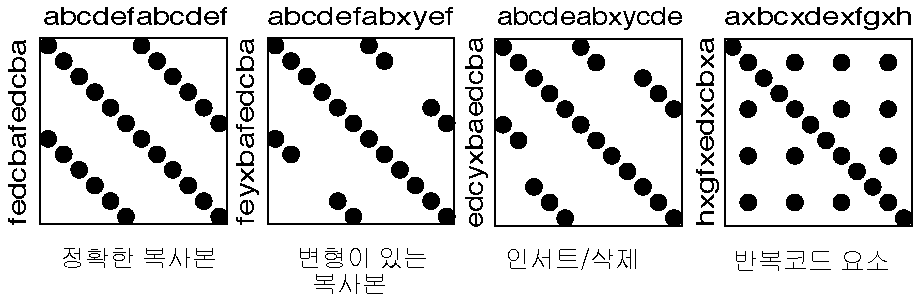
\includegraphics[width=\textwidth]{DuplicationDotplot}
\caption{Possible sequences of dot and their associated interpretations.}
\figlabel{DuplicationDotplot}
\end{center}
\end{figure}

Some interesting configurations formed by the dots in the matrices are the following:

\begin{bulletlist}
\item \emph{Exact Copies:} diagonals of dots indicate copied sequences of source code.

\item \emph{Copies With Variations:} sequences that have holes in them indicate that a portion of a copied sequences has been changed.

\item \emph{Inserts/Deletes:} broken sequences with parts shifted to the right or left indicate that a portion of code has been inserted or deleted.

\item \emph{Repetitive Code Elements:} rectangular configurations indicate periodic occurrences of the same code. An example is the break at the end of the individual cases of a C or C ++ switch statement, or recurring preprocessor commands like \lct{\#ifdef SOME CONDITION}.
\end{bulletlist}

\subsection*{Tradeoffs}

\subsubsection*{Pros}

\begin{bulletlist}
\item The approach is largely language-independent, since only the code normalization depends on the language syntax.

\item The approach works well when reverse engineering large amounts of unknown code, because the dotplots attract your eye to certain parts of the code to be studied more closely.

\item The idea is simple yet works surprisingly well. A simple version of the approach can be implemented by a good programmer using a appropriate tools in a couple of days. (One of our better students made a small dotplot browser in Delphi in two days.)
\end{bulletlist}

\subsubsection*{Cons}

\begin{bulletlist}
\item Dotplots only present pairwise comparisons. They do not necessarily help you identify all instances of duplicated elements in the entire software system. Although the approach can easily be extended to present multiple files across each axis, the comparisons are still only pairwise.
\end{bulletlist}

\subsubsection*{Difficulties}

\begin{bulletlist}
\item A naive implementation of a dotplot visualizer may not scale well to large systems. Tuning and optimizing the approach for large data sets can compromise the simplicity of the approach.

\begin{figure}[t]
\begin{center}
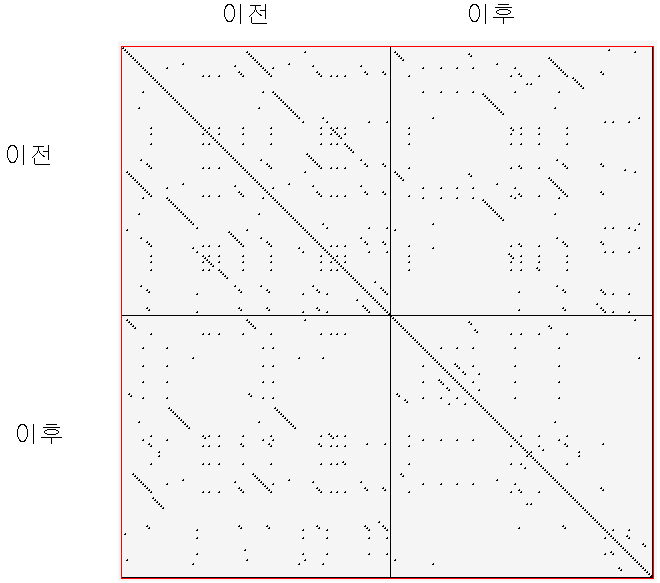
\includegraphics[width=0.8\textwidth]{DuplicationRefactoring}
\caption{Code duplication before and after refactoring.}
\figlabel{DuplicationRefactoring}
\end{center}
\end{figure}

\item The interpretation of the data may be more subtle than it appears at first glance. Indeed, while comparing multiple files the diagonals represent more duplication than is really in the system because we are comparing duplicated fragments with themselves over different files, as shown by \figref{DuplicationRefactoring} and \figref{DuplicationPython}.

\index{mural visualization}
\item The screen size limits the amount of information that can be visualized. Some success has been achieved with so-called ``mural'' visualization approaches \cite{Jerd96b}. However, these techniques are significantly more difficult to implement than simple dotplots and are not worth the extra effort.
\end{bulletlist}

\subsection*{Example}

In \figref{DuplicationRefactoring} we see a \ind{dotplot} of two versions of a piece of software, before and after the duplication has been removed. The first version is compared to itself in the top left square. The line down the diagonal simply shows us that every line of code is being compared to itself. What is more interesting is that several other diagonal lines occur in the dotplot, which means that code has been duplicated within this file. A second version of the same file is compared to itself in the lower right square. Here we see no significant duplication aside from the main diagonal, which reflects the fact that all the duplicated code has been successfully refactored.

\begin{figure}[h]
\begin{center}
\includegraphics[width=\textwidth]{DuplicationPython}
\caption{A Python file A being compared to itself and to a second file B.}
\figlabel{DuplicationPython}
\end{center}
\end{figure}

The bottom left and top right squares are mirror images of each other. They tell us how the before and after files have been reorganized. Since there is no strong diagonal, this tells us that significant reorganization has taken place. The diagonal stripes show us which parts of the old version have survived and where they appear in the new version. From the dotplot alone, we can guess that about half of the code has survived, and another half of the code has been significantly rewritten.

Dotplots are also useful to detect duplication across multiple files. \figref{DuplicationPython} shows a dotplot comparing two \ind{Python} files. The comparison of A vs. A shows that there is essentially no internal duplication. Very likely there are some switch statements in the bottom have of the file, indicated by the matrix pattern.

When we compare file A to file B, however, we detect a staggering amount of duplication. It looks very much like file B is just a copy of file A that has been extended in various ways. Closer investigation showed this to be the case. In fact, file A was just an older version of file B that had inadvertently been left in the release.

Dotplots can also be useful to detect other problems. \figref{DuplicationSwitch} presents four clones that represent a switch statement over a type variable that is used to call individual construction code. The duplicated code could perhaps be eliminated by applying \charef{Transform Conditionals to Polymorphism}{TransformConditionalsToPolymorphism}.

\begin{figure}
\begin{center}
\includegraphics[width=0.75\textwidth]{DuplicationSwitch}
\caption{Dotplots produced by four switch statements.}
\figlabel{DuplicationSwitch}
\end{center}
\end{figure}

\subsection*{Known Uses}

The pattern has been applied in biological research to detect DNA sequences \cite{Pust82a}. The Dotplot tool \cite{Helf95a} has been used to detect similarities in manual pages, literary texts and names from file systems. In the \ind{FAMOOS} project, the pattern has been applied to build \ind{Duploc}, a tool for identifying duplication in software source code \cite{Duca99b}. The \ind{Dup} tool \cite{Bake92a} has been used to investigated the source code of the X-Window system and uses a dotplot matrix graphical representation.

\subsection*{Related Patterns}

Once you have detected duplicated code, numerous refactoring patterns may apply, in particular \patpgref{Extract Method}{ExtractMethod}.

Very often duplicated code arises because clients assume too many responsibilities. In that case, \patpgref{Move Behavior Close to Data}{MoveBehaviorCloseToData} will help you to eliminate the duplication.

Dotplots also help to detect large conditional constructs. You should probably \charef{Transform Conditionals to Polymorphism}{TransformConditionalsToPolymorphism} to eliminate these conditionals and thereby achieve a more flexible design. 

%=============================================================
\ifx\wholebook\relax\else
   \bibliographystyle{alpha}
   \bibliography{scg}
   \end{document}
\fi
%=============================================================


% $Author: oscar $
% $Date: 2009-09-15 16:53:48 +0200 (Tue, 15 Sep 2009) $
% $Revision: 29111 $
%=================================================================
\ifx\wholebook\relax\else
% --------------------------------------------
% Lulu:
	\documentclass[a4paper,10pt,twoside]{book}
	\usepackage[
		papersize={6.13in,9.21in},
		hmargin={.815in,.815in},
		vmargin={.98in,.98in},
		ignoreheadfoot
	]{geometry}
	\usepackage[hangul]{kotex}
	% $Author: oscar $
% $Date: 2009-09-13 20:58:29 +0200 (Sun, 13 Sep 2009) $
% $Revision: 29070 $
%=============================================================
% NB: documentclass must be set in main document.
% Allows book to be generated in multiple formats.
%=============================================================
%:Packages
\usepackage[T1]{fontenc}  %%%%%really important to get the code directly in the text!
\usepackage{palatino}
\usepackage{ifthen}
\usepackage{graphicx}
\graphicspath{{figures/}}
\usepackage{xspace}
\usepackage{makeidx}
\usepackage{isodateo} % enable \isodate
\usepackage{amssymb,textcomp}
%=============================================================
%:More packages
%\usepackage[english]{babel}
%\usepackage{lmodern}
%\usepackage[scaled=0.85]{helvet}
%\usepackage{microtype}
%\usepackage{theorem}
%\usepackage{float}
%\usepackage{longtable}
%\usepackage[nottoc]{tocbibind}
%\usepackage{multicol}
%\usepackage{booktabs}	% book-style tables
%\usepackage{topcapt}	% enables \topcaption
%\usepackage{multirow}
%\usepackage{tabularx}
%\usepackage{alltt}
\usepackage[usenames,dvipsnames]{color}
%\usepackage[hang]{subfigure}\makeatletter\def\p@subfigure{\thefigure\,}\makeatother
%\usepackage{rotating}
%\usepackage{enumitem}	% apb: allows more control over tags in enumerations
%\usepackage{verbatim}     % for comment environment
%\usepackage{varioref}	% for page references that work
%\usepackage{needspace}
%\usepackage[newparttoc]{titlesec}
%\usepackage{titletoc}
%\usepackage{wrapfig}
\usepackage[
	colorlinks=true,
	linkcolor=black,
	urlcolor=black,
	citecolor=black
]{hyperref}   % should come last
%=============================================================
%:URL style
\makeatletter
\def\url@leostyle{%
  \@ifundefined{selectfont}{\def\UrlFont{\sf}}{\def\UrlFont{\sffamily}}}
\makeatother
\urlstyle{leo}
%=============================================================
%:Booleans
\newboolean{lulu}
\setboolean{lulu}{false}
\newcommand{\ifluluelse}[2]{\ifthenelse{\boolean{lulu}}{#1}{#2}}
%=============================================================
%:Editorial comment macros
\newcommand{\nnbb}[2]{
  \fbox{\bfseries\sffamily\scriptsize#1}
  {\sf\small$\blacktriangleright$\textit{#2}$\blacktriangleleft$}
}
\newcommand{\on}[1]{\nnbb{Oscar}{#1}}
\newcommand{\here}{\nnbb{CONTINUE}{HERE}}
%=============================================================
%:Abbreviation macros
\newcommand{\ie}{\emph{i.e.},\xspace}
\newcommand{\eg}{\emph{e.g.},\xspace}
\newcommand{\etc}{\emph{etc.}\xspace}
\newcommand{\etal}{\emph{et al.}\xspace}
\newcommand{\straightquote}{"}
\newcommand{\sba}{\url{SquareBracketAssociates.org}\xspace}
%=============================================================
%:Patterns
% \newcommand{\pattern}[2]{\newpage\section{{\sf #1}}\label{pat:#2}}
% \newcommand{\pattern}[2]{\newpage\index{#1 (Pattern)}\section{#1}\label{pat:#2}}
\newcommand{\pattern}[2]{\cleardoublepage\index{#1 (패턴)}\section{#1}\label{pat:#2}}
\newcommand{\thumbnail}[2]{\index{#1 (패턴)}\subsection{#1}\label{pat:#2}}
\newcommand{\thumblang}[2]{\index{#1 (패턴 랭귀지)}\subsection{#1}\label{pat:#2}}
\newcommand{\variant}[1]{{\emph{#1}}\xspace}
% \newcommand{\problem}[1]{\subsection*{Problem}\emph{#1}}
\newcommand{\intent}[1]{\paragraph{의도}\emph{#1}}
\newcommand{\problem}[1]{\paragraph{문제}\emph{#1}}
\newcommand{\solution}[1]{\paragraph{해결}\emph{#1}}
\newcommand{\discussion}[0]{\paragraph{토론}}
\newcommand{\cmd}[1]{{\tt #1}\xspace}
%=============================================================
%:Environments
\newenvironment{bulletlist}{\begin{itemize}\setlength{\itemsep}{0ex}}
{\end{itemize}}
%=============================================================
%:Cross reference macros
\newcommand{\chalabel}[1]{\label{cha:#1}}
\newcommand{\seclabel}[1]{\label{sec:#1}}
\newcommand{\figlabel}[1]{\label{fig:#1}}
\newcommand{\tablabel}[1]{\label{tab:#1}}
\newcommand{\rulelabel}[1]{\label{rule:#1}}
\newcommand{\eglabel}[1]{\label{eg:#1}}
\newcommand{\scrlabel}[1]{\label{scr:#1}}
\newcommand{\mthlabel}[1]{\label{mth:#1}}
\newcommand{\clslabel}[1]{\label{cls:#1}}
\newcommand{\faqlabel}[1]{\label{faq:#1}}
%\newcommand{\charef}[1]{Chapter~\ref{cha:#1}\xspace}
%\newcommand{\secref}[1]{Section~\ref{sec:#1}\xspace}
\newcommand{\figref}[1]{Figure~\ref{fig:#1}\xspace}
% \newcommand{\patpgref}[2]{\hyperref[pat:#2]{\sf #1} [p.~\pageref{pat:#2}]\xspace}
\newcommand{\patpgref}[2]{\index{#1 (Pattern)}\hyperref[pat:#2]{#1} [p.~\pageref{pat:#2}]\xspace}
\newcommand{\patlangpgref}[2]{\index{#1 (Pattern language)}\hyperref[pat:#2]{#1} [p.~\pageref{pat:#2}]\xspace}
% \newcommand{\patref}[2]{\hyperref[pat:#2]{\sf #1}\xspace}
\newcommand{\patref}[2]{\index{#1 (Pattern)}\hyperref[pat:#2]{#1}\xspace}
\newcommand{\patlangref}[2]{\index{#1 (Pattern language)}\hyperref[pat:#2]{#1}\xspace}
% \newcommand{\charef}[2]{\hyperref[cha:#2]{\underline{\sf #1}}\xspace}
% \newcommand{\charef}[2]{\hyperref[cha:#2]{\sf #1}\xspace}
\newcommand{\charef}[2]{\index{#1 (Pattern cluster)}\hyperref[cha:#2]{#1}\xspace}
% \newcommand{\chapgref}[2]{\hyperref[cha:#2]{\sf #1} [p.~\pageref{cha:#2}]\xspace}
\newcommand{\chapgref}[2]{\index{#1 (Pattern cluster)}\hyperref[cha:#2]{#1} [p.~\pageref{cha:#2}]\xspace}
%\newcommand{\Figref}[1]{Figure~\ref{fig:#1}\xspace}
%\newcommand{\appref}[1]{Appendix~\ref{app:#1}\xspace}
%\newcommand{\tabref}[1]{Table~\ref{tab:#1}\xspace}
%\newcommand{\ruleref}[1]{\ref{rule:#1}\xspace}
%\newcommand{\egref}[1]{example~\ref{eg:#1}\xspace}
%\newcommand{\Egref}[1]{Example~\ref{eg:#1}\xspace}
%\newcommand{\scrref}[1]{script~\ref{scr:#1}\xspace}
%\newcommand{\Scrref}[1]{Script~\ref{scr:#1}\xspace}
%\newcommand{\tscrref}[1]{the script~\ref{scr:#1}\xspace}
%\newcommand{\Tscrref}[1]{The script~\ref{scr:#1}\xspace}
%\newcommand{\mthref}[1]{method~\ref{mth:#1}\xspace}
%\newcommand{\mthsref}[1]{methods~\ref{mth:#1}\xspace}
%\newcommand{\Mthref}[1]{Method~\ref{mth:#1}\xspace}
%\newcommand{\tmthref}[1]{the method~\ref{mth:#1}\xspace}
%\newcommand{\Tmthref}[1]{The method~\ref{mth:#1}\xspace}
%\newcommand{\clsref}[1]{class~\ref{cls:#1}\xspace}
%\newcommand{\tclsref}[1]{the class~\ref{cls:#1}\xspace}
%\newcommand{\Tclsref}[1]{The class~\ref{cls:#1}\xspace}
%=============================================================
%:Page Layout
\setlength{\headsep}{1cm}
%=============================================================
%:Menu item macro
%\definecolor{lightgray}{gray}{0.89}
%\newcommand{\menu}[1]{{%
%	\setlength{\fboxsep}{0pt}%
%	\colorbox{lightgray}{{{\upshape\sffamily\strut \,#1\,}}}}}
%\newcommand{\go}{\,$\triangleright$\,}
%\newcommand{\short}[1]{\mbox{{\sc cmd}\hspace{0.08em}--\hspace{0.09em}#1}\xspace}
%\newcommand{\button}[1]{{%
%	\setlength{\fboxsep}{0pt}%
%	\fbox{{\upshape\sffamily\strut \,#1\,}}}}
%\newcommand{\toolsflap}{\textit{Tools} flap\xspace}
%=============================================================
%:Section depth
%\setcounter{secnumdepth}{2}
%
%\DeclareGraphicsExtensions{.pdf, .jpg, .png}
%=============================================================
%:PDF setup
\hypersetup{
   pdftitle={Object-Oriented Reengineering Patterns},
   pdfauthor={Serge Demeyer, St\'ephane Ducasse, Oscar Nierstrasz},
   pdfkeywords={Reengineering, Object-Oriented Programming, Patterns},
   pdfsubject={Computer Science}
}
%=============================================================
%:Page layout and appearance
%\renewcommand{\chaptermark}[1]{\markboth{#1}{}}
%\renewcommand{\sectionmark}[1]{\markright{\thesection\ #1}}
%\renewpagestyle{plain}[\small\itshape]{%
%	\setheadrule{0pt}%
%	\sethead[][][]{}{}{}%
%	\setfoot[][][]{}{}{}}
%\renewpagestyle{headings}[\small\itshape]{%
%	\setheadrule{0pt}%
%	\setmarks{chapter}{section}%
%	\sethead[\thepage][][\chaptertitle]{\sectiontitle}{}{\thepage}%
%	\setfoot[][][]{}{}{}}
%=============================================================
%:Title section setup and TOC numbering depth
%\setcounter{secnumdepth}{1}
%\setcounter{tocdepth}{1}
%\titleformat{\part}[display]{\centering}{\huge\partname\ \thepart}{1em}{\Huge\textbf}[]
%\titleformat{\chapter}[display]{}{\huge\chaptertitlename\ \thechapter}{1em}{\Huge\raggedright\textbf}[]
%\titlecontents{part}[3pc]{%
%		\pagebreak[2]\addvspace{1em plus.4em minus.2em}%
%		\leavevmode\large\bfseries}
%	{\contentslabel{3pc}}{\hspace*{-3pc}}
%	{}[\nopagebreak]
%\titlecontents{chapter}[3pc]{%
%		\pagebreak[0]\addvspace{1em plus.2em minus.2em}%
%		\leavevmode\bfseries}
%	{\contentslabel{3pc}}{}
%	{\hfill\contentspage}[\nopagebreak]
%\dottedcontents{section}[3pc]{}{3pc}{1pc}
%\dottedcontents{subsection}[3pc]{}{0pc}{1pc}
%\let\origdoublepage\cleardoublepage
%\newcommand{\clearemptydoublepage}{%
%  \clearpage
%  {\pagestyle{empty}\origdoublepage}}
%\let\cleardoublepage\clearemptydoublepage % see http://www.tex.ac.uk/cgi-bin/texfaq2html?label=patch
%=============================================================
%:Listings package configuration
\newcommand{\caret}{\makebox{\raisebox{0.4ex}{\footnotesize{$\wedge$}}}}
% \newcommand{\escape}{{\sf \textbackslash}}
\definecolor{source}{gray}{0.95}
\usepackage{listings}
\lstdefinelanguage{Smalltalk}{
  morestring=[d]',
% Adapt this to other languages!
%  morecomment=[s]{"}{"},
  alsoletter={\#:},
  %escapechar={!},
  literate=
    {BANG}{!}1
%    {UNDERSCORE}{\_}1
    {\\st}{Smalltalk}9 % convenience -- in case \st occurs in code
    % {'}{{\textquotesingle}}1 % replaced by upquote=true in \lstset
%    {_}{{$\leftarrow$}}1
    {>>>}{{\sep}}1
    {^}{{$\uparrow$}}1
    {~}{{$\sim$}}1
    {-}{{\sf -\hspace{-0.13em}-}}1  % the goal is to make - the same width as +
    {+}{\raisebox{0.08ex}{+}}1		% and to raise + off the baseline to match -
    {-->}{{\quad$\longrightarrow$\quad}}3
	, % Don't forget the comma at the end!
  tabsize=4
}[keywords,comments,strings]

\lstset{language=Smalltalk,
	basicstyle=\sffamily,
	keywordstyle=\color{black}\bfseries,
	% stringstyle=\ttfamily, % Ugly! do we really want this? -- on
	mathescape=true,
	showstringspaces=false,
	keepspaces=true,
	breaklines=true,
	breakautoindent=true,
	backgroundcolor=\color{source},
	lineskip={-1pt}, % Ugly hack
	upquote=true, % straight quote; requires textcomp package
	columns=fullflexible} % no fixed width fonts
% \newcommand{\ct}{\lstinline[mathescape=false,basicstyle={\sffamily\upshape}]}
\newcommand{\ct}{\lstinline[mathescape=false,backgroundcolor=\color{white},basicstyle={\sffamily\upshape}]}
\newcommand{\lct}[1]{{\textsf{\textup{#1}}}}
%\newcommand{\scat}[1]{\emph{\textsf{#1}}\xspace}
%\newcommand{\prot}[1]{\emph{\textsf{#1}}\xspace}
% NB: No argument!
\lstnewenvironment{code}[0]{%
	\lstset{%
		% frame=lines,
		frame=single,
		framerule=0pt,
		mathescape=false
	}
}{}
%\def\ignoredollar#1{}
%=============================================================
%:Reserving space
%\newcommand{\needlines}[1]{\Needspace{#1\baselineskip}}
%=============================================================
%:Indexing macros
% Macros ending with "ind" generate text as well as an index entry
% Macros ending with "index" *only* generate an index entry
\newcommand{\ind}[1]{\index{#1}#1\xspace} % plain text
\newcommand{\subind}[2]{\index{#1!#2}#2\xspace} % show #2, subindex under #1
\newcommand{\emphind}[1]{\index{#1}\emph{#1}\xspace} % emph #1
\newcommand{\emphsubind}[2]{\index{#1!#2}\emph{#2}\xspace} % show emph #2, subindex under #1
\newcommand{\patind}[1]{\index{#1@#1 (pattern)}\ct{#1}\xspace} % pattern
\newcommand{\seeindex}[2]{\index{#1|see{#2}}} % #1, see #2
%\newcommand{\boldidx}[1]{{\bf #1}} % breaks hyperlink
%\newcommand{\indmain}[1]{\index{#1}#1\xspace} 
%\newcommand{\emphsubindmain}[2]{\index{#1!#2}\emph{#2}\xspace} % subindex, main entry
%\newcommand{\subindmain}[2]{\index{#1!#2}#2\xspace} % subindex, main entry
%\newcommand{\clsindmain}[1]{\index{#1!\#@(class)}\ct{#1}\xspace} % class main
%\newcommand{\indexmain}[1]{\index{#1}} 
%=============================================================
\parskip 1ex
%=============================================================

	\pagestyle{headings}
	\setboolean{lulu}{true}
% --------------------------------------------
% A4:
%	\documentclass[a4paper,11pt,twoside]{book}
%	% $Author: oscar $
% $Date: 2009-09-13 20:58:29 +0200 (Sun, 13 Sep 2009) $
% $Revision: 29070 $
%=============================================================
% NB: documentclass must be set in main document.
% Allows book to be generated in multiple formats.
%=============================================================
%:Packages
\usepackage[T1]{fontenc}  %%%%%really important to get the code directly in the text!
\usepackage{palatino}
\usepackage{ifthen}
\usepackage{graphicx}
\graphicspath{{figures/}}
\usepackage{xspace}
\usepackage{makeidx}
\usepackage{isodateo} % enable \isodate
\usepackage{amssymb,textcomp}
%=============================================================
%:More packages
%\usepackage[english]{babel}
%\usepackage{lmodern}
%\usepackage[scaled=0.85]{helvet}
%\usepackage{microtype}
%\usepackage{theorem}
%\usepackage{float}
%\usepackage{longtable}
%\usepackage[nottoc]{tocbibind}
%\usepackage{multicol}
%\usepackage{booktabs}	% book-style tables
%\usepackage{topcapt}	% enables \topcaption
%\usepackage{multirow}
%\usepackage{tabularx}
%\usepackage{alltt}
\usepackage[usenames,dvipsnames]{color}
%\usepackage[hang]{subfigure}\makeatletter\def\p@subfigure{\thefigure\,}\makeatother
%\usepackage{rotating}
%\usepackage{enumitem}	% apb: allows more control over tags in enumerations
%\usepackage{verbatim}     % for comment environment
%\usepackage{varioref}	% for page references that work
%\usepackage{needspace}
%\usepackage[newparttoc]{titlesec}
%\usepackage{titletoc}
%\usepackage{wrapfig}
\usepackage[
	colorlinks=true,
	linkcolor=black,
	urlcolor=black,
	citecolor=black
]{hyperref}   % should come last
%=============================================================
%:URL style
\makeatletter
\def\url@leostyle{%
  \@ifundefined{selectfont}{\def\UrlFont{\sf}}{\def\UrlFont{\sffamily}}}
\makeatother
\urlstyle{leo}
%=============================================================
%:Booleans
\newboolean{lulu}
\setboolean{lulu}{false}
\newcommand{\ifluluelse}[2]{\ifthenelse{\boolean{lulu}}{#1}{#2}}
%=============================================================
%:Editorial comment macros
\newcommand{\nnbb}[2]{
  \fbox{\bfseries\sffamily\scriptsize#1}
  {\sf\small$\blacktriangleright$\textit{#2}$\blacktriangleleft$}
}
\newcommand{\on}[1]{\nnbb{Oscar}{#1}}
\newcommand{\here}{\nnbb{CONTINUE}{HERE}}
%=============================================================
%:Abbreviation macros
\newcommand{\ie}{\emph{i.e.},\xspace}
\newcommand{\eg}{\emph{e.g.},\xspace}
\newcommand{\etc}{\emph{etc.}\xspace}
\newcommand{\etal}{\emph{et al.}\xspace}
\newcommand{\straightquote}{"}
\newcommand{\sba}{\url{SquareBracketAssociates.org}\xspace}
%=============================================================
%:Patterns
% \newcommand{\pattern}[2]{\newpage\section{{\sf #1}}\label{pat:#2}}
% \newcommand{\pattern}[2]{\newpage\index{#1 (Pattern)}\section{#1}\label{pat:#2}}
\newcommand{\pattern}[2]{\cleardoublepage\index{#1 (패턴)}\section{#1}\label{pat:#2}}
\newcommand{\thumbnail}[2]{\index{#1 (패턴)}\subsection{#1}\label{pat:#2}}
\newcommand{\thumblang}[2]{\index{#1 (패턴 랭귀지)}\subsection{#1}\label{pat:#2}}
\newcommand{\variant}[1]{{\emph{#1}}\xspace}
% \newcommand{\problem}[1]{\subsection*{Problem}\emph{#1}}
\newcommand{\intent}[1]{\paragraph{의도}\emph{#1}}
\newcommand{\problem}[1]{\paragraph{문제}\emph{#1}}
\newcommand{\solution}[1]{\paragraph{해결}\emph{#1}}
\newcommand{\discussion}[0]{\paragraph{토론}}
\newcommand{\cmd}[1]{{\tt #1}\xspace}
%=============================================================
%:Environments
\newenvironment{bulletlist}{\begin{itemize}\setlength{\itemsep}{0ex}}
{\end{itemize}}
%=============================================================
%:Cross reference macros
\newcommand{\chalabel}[1]{\label{cha:#1}}
\newcommand{\seclabel}[1]{\label{sec:#1}}
\newcommand{\figlabel}[1]{\label{fig:#1}}
\newcommand{\tablabel}[1]{\label{tab:#1}}
\newcommand{\rulelabel}[1]{\label{rule:#1}}
\newcommand{\eglabel}[1]{\label{eg:#1}}
\newcommand{\scrlabel}[1]{\label{scr:#1}}
\newcommand{\mthlabel}[1]{\label{mth:#1}}
\newcommand{\clslabel}[1]{\label{cls:#1}}
\newcommand{\faqlabel}[1]{\label{faq:#1}}
%\newcommand{\charef}[1]{Chapter~\ref{cha:#1}\xspace}
%\newcommand{\secref}[1]{Section~\ref{sec:#1}\xspace}
\newcommand{\figref}[1]{Figure~\ref{fig:#1}\xspace}
% \newcommand{\patpgref}[2]{\hyperref[pat:#2]{\sf #1} [p.~\pageref{pat:#2}]\xspace}
\newcommand{\patpgref}[2]{\index{#1 (Pattern)}\hyperref[pat:#2]{#1} [p.~\pageref{pat:#2}]\xspace}
\newcommand{\patlangpgref}[2]{\index{#1 (Pattern language)}\hyperref[pat:#2]{#1} [p.~\pageref{pat:#2}]\xspace}
% \newcommand{\patref}[2]{\hyperref[pat:#2]{\sf #1}\xspace}
\newcommand{\patref}[2]{\index{#1 (Pattern)}\hyperref[pat:#2]{#1}\xspace}
\newcommand{\patlangref}[2]{\index{#1 (Pattern language)}\hyperref[pat:#2]{#1}\xspace}
% \newcommand{\charef}[2]{\hyperref[cha:#2]{\underline{\sf #1}}\xspace}
% \newcommand{\charef}[2]{\hyperref[cha:#2]{\sf #1}\xspace}
\newcommand{\charef}[2]{\index{#1 (Pattern cluster)}\hyperref[cha:#2]{#1}\xspace}
% \newcommand{\chapgref}[2]{\hyperref[cha:#2]{\sf #1} [p.~\pageref{cha:#2}]\xspace}
\newcommand{\chapgref}[2]{\index{#1 (Pattern cluster)}\hyperref[cha:#2]{#1} [p.~\pageref{cha:#2}]\xspace}
%\newcommand{\Figref}[1]{Figure~\ref{fig:#1}\xspace}
%\newcommand{\appref}[1]{Appendix~\ref{app:#1}\xspace}
%\newcommand{\tabref}[1]{Table~\ref{tab:#1}\xspace}
%\newcommand{\ruleref}[1]{\ref{rule:#1}\xspace}
%\newcommand{\egref}[1]{example~\ref{eg:#1}\xspace}
%\newcommand{\Egref}[1]{Example~\ref{eg:#1}\xspace}
%\newcommand{\scrref}[1]{script~\ref{scr:#1}\xspace}
%\newcommand{\Scrref}[1]{Script~\ref{scr:#1}\xspace}
%\newcommand{\tscrref}[1]{the script~\ref{scr:#1}\xspace}
%\newcommand{\Tscrref}[1]{The script~\ref{scr:#1}\xspace}
%\newcommand{\mthref}[1]{method~\ref{mth:#1}\xspace}
%\newcommand{\mthsref}[1]{methods~\ref{mth:#1}\xspace}
%\newcommand{\Mthref}[1]{Method~\ref{mth:#1}\xspace}
%\newcommand{\tmthref}[1]{the method~\ref{mth:#1}\xspace}
%\newcommand{\Tmthref}[1]{The method~\ref{mth:#1}\xspace}
%\newcommand{\clsref}[1]{class~\ref{cls:#1}\xspace}
%\newcommand{\tclsref}[1]{the class~\ref{cls:#1}\xspace}
%\newcommand{\Tclsref}[1]{The class~\ref{cls:#1}\xspace}
%=============================================================
%:Page Layout
\setlength{\headsep}{1cm}
%=============================================================
%:Menu item macro
%\definecolor{lightgray}{gray}{0.89}
%\newcommand{\menu}[1]{{%
%	\setlength{\fboxsep}{0pt}%
%	\colorbox{lightgray}{{{\upshape\sffamily\strut \,#1\,}}}}}
%\newcommand{\go}{\,$\triangleright$\,}
%\newcommand{\short}[1]{\mbox{{\sc cmd}\hspace{0.08em}--\hspace{0.09em}#1}\xspace}
%\newcommand{\button}[1]{{%
%	\setlength{\fboxsep}{0pt}%
%	\fbox{{\upshape\sffamily\strut \,#1\,}}}}
%\newcommand{\toolsflap}{\textit{Tools} flap\xspace}
%=============================================================
%:Section depth
%\setcounter{secnumdepth}{2}
%
%\DeclareGraphicsExtensions{.pdf, .jpg, .png}
%=============================================================
%:PDF setup
\hypersetup{
   pdftitle={Object-Oriented Reengineering Patterns},
   pdfauthor={Serge Demeyer, St\'ephane Ducasse, Oscar Nierstrasz},
   pdfkeywords={Reengineering, Object-Oriented Programming, Patterns},
   pdfsubject={Computer Science}
}
%=============================================================
%:Page layout and appearance
%\renewcommand{\chaptermark}[1]{\markboth{#1}{}}
%\renewcommand{\sectionmark}[1]{\markright{\thesection\ #1}}
%\renewpagestyle{plain}[\small\itshape]{%
%	\setheadrule{0pt}%
%	\sethead[][][]{}{}{}%
%	\setfoot[][][]{}{}{}}
%\renewpagestyle{headings}[\small\itshape]{%
%	\setheadrule{0pt}%
%	\setmarks{chapter}{section}%
%	\sethead[\thepage][][\chaptertitle]{\sectiontitle}{}{\thepage}%
%	\setfoot[][][]{}{}{}}
%=============================================================
%:Title section setup and TOC numbering depth
%\setcounter{secnumdepth}{1}
%\setcounter{tocdepth}{1}
%\titleformat{\part}[display]{\centering}{\huge\partname\ \thepart}{1em}{\Huge\textbf}[]
%\titleformat{\chapter}[display]{}{\huge\chaptertitlename\ \thechapter}{1em}{\Huge\raggedright\textbf}[]
%\titlecontents{part}[3pc]{%
%		\pagebreak[2]\addvspace{1em plus.4em minus.2em}%
%		\leavevmode\large\bfseries}
%	{\contentslabel{3pc}}{\hspace*{-3pc}}
%	{}[\nopagebreak]
%\titlecontents{chapter}[3pc]{%
%		\pagebreak[0]\addvspace{1em plus.2em minus.2em}%
%		\leavevmode\bfseries}
%	{\contentslabel{3pc}}{}
%	{\hfill\contentspage}[\nopagebreak]
%\dottedcontents{section}[3pc]{}{3pc}{1pc}
%\dottedcontents{subsection}[3pc]{}{0pc}{1pc}
%\let\origdoublepage\cleardoublepage
%\newcommand{\clearemptydoublepage}{%
%  \clearpage
%  {\pagestyle{empty}\origdoublepage}}
%\let\cleardoublepage\clearemptydoublepage % see http://www.tex.ac.uk/cgi-bin/texfaq2html?label=patch
%=============================================================
%:Listings package configuration
\newcommand{\caret}{\makebox{\raisebox{0.4ex}{\footnotesize{$\wedge$}}}}
% \newcommand{\escape}{{\sf \textbackslash}}
\definecolor{source}{gray}{0.95}
\usepackage{listings}
\lstdefinelanguage{Smalltalk}{
  morestring=[d]',
% Adapt this to other languages!
%  morecomment=[s]{"}{"},
  alsoletter={\#:},
  %escapechar={!},
  literate=
    {BANG}{!}1
%    {UNDERSCORE}{\_}1
    {\\st}{Smalltalk}9 % convenience -- in case \st occurs in code
    % {'}{{\textquotesingle}}1 % replaced by upquote=true in \lstset
%    {_}{{$\leftarrow$}}1
    {>>>}{{\sep}}1
    {^}{{$\uparrow$}}1
    {~}{{$\sim$}}1
    {-}{{\sf -\hspace{-0.13em}-}}1  % the goal is to make - the same width as +
    {+}{\raisebox{0.08ex}{+}}1		% and to raise + off the baseline to match -
    {-->}{{\quad$\longrightarrow$\quad}}3
	, % Don't forget the comma at the end!
  tabsize=4
}[keywords,comments,strings]

\lstset{language=Smalltalk,
	basicstyle=\sffamily,
	keywordstyle=\color{black}\bfseries,
	% stringstyle=\ttfamily, % Ugly! do we really want this? -- on
	mathescape=true,
	showstringspaces=false,
	keepspaces=true,
	breaklines=true,
	breakautoindent=true,
	backgroundcolor=\color{source},
	lineskip={-1pt}, % Ugly hack
	upquote=true, % straight quote; requires textcomp package
	columns=fullflexible} % no fixed width fonts
% \newcommand{\ct}{\lstinline[mathescape=false,basicstyle={\sffamily\upshape}]}
\newcommand{\ct}{\lstinline[mathescape=false,backgroundcolor=\color{white},basicstyle={\sffamily\upshape}]}
\newcommand{\lct}[1]{{\textsf{\textup{#1}}}}
%\newcommand{\scat}[1]{\emph{\textsf{#1}}\xspace}
%\newcommand{\prot}[1]{\emph{\textsf{#1}}\xspace}
% NB: No argument!
\lstnewenvironment{code}[0]{%
	\lstset{%
		% frame=lines,
		frame=single,
		framerule=0pt,
		mathescape=false
	}
}{}
%\def\ignoredollar#1{}
%=============================================================
%:Reserving space
%\newcommand{\needlines}[1]{\Needspace{#1\baselineskip}}
%=============================================================
%:Indexing macros
% Macros ending with "ind" generate text as well as an index entry
% Macros ending with "index" *only* generate an index entry
\newcommand{\ind}[1]{\index{#1}#1\xspace} % plain text
\newcommand{\subind}[2]{\index{#1!#2}#2\xspace} % show #2, subindex under #1
\newcommand{\emphind}[1]{\index{#1}\emph{#1}\xspace} % emph #1
\newcommand{\emphsubind}[2]{\index{#1!#2}\emph{#2}\xspace} % show emph #2, subindex under #1
\newcommand{\patind}[1]{\index{#1@#1 (pattern)}\ct{#1}\xspace} % pattern
\newcommand{\seeindex}[2]{\index{#1|see{#2}}} % #1, see #2
%\newcommand{\boldidx}[1]{{\bf #1}} % breaks hyperlink
%\newcommand{\indmain}[1]{\index{#1}#1\xspace} 
%\newcommand{\emphsubindmain}[2]{\index{#1!#2}\emph{#2}\xspace} % subindex, main entry
%\newcommand{\subindmain}[2]{\index{#1!#2}#2\xspace} % subindex, main entry
%\newcommand{\clsindmain}[1]{\index{#1!\#@(class)}\ct{#1}\xspace} % class main
%\newcommand{\indexmain}[1]{\index{#1}} 
%=============================================================
\parskip 1ex
%=============================================================

%	\usepackage{a4wide}
% --------------------------------------------
	\begin{document}
	\renewcommand{\nnbb}[2]{} % Disable editorial comments
	\sloppy
\fi
%=================================================================
\chapter{책임 재배포}
\chalabel{RedistributeResponsibilities}

\index{God Class}
\index{data container}
You are responsible for reengineering the information system that manages all employee records for a large public administration. Due to recent political upheavals, you know that there will be many changes required in the system to cope with privatization, new laws, and new regulations, but you do not know exactly what they will be. The existing system consists of a nominally object-oriented reimplementation of an older procedural system. The code contains many pseudo-objects: data containers masquerading as objects, and big, procedural ``god classes'' that implement most of a the logic of individual subsystems. One class, called \lct{TaxRevision2000}, has a single method consisting essentially of a case statement that is 3000 lines long.

As long as the system was relatively stable, this design posed no particular problems, but now you see that even relatively modest changes to system require months of planning, testing and debugging due to weak encapsulation of data. You are convinced that migrating to a more object-oriented design will make the system more robust and easier to adapt to future requirements. But how do you know where the problems lie? Which responsibilities should be redistributed? Which data containers should you redesign, which ones should you wrap, and which ones are better left alone?

\subsection*{Forces}

\begin{bulletlist}
\item Data containers (objects that just provide access to data, but no own behavior) are a simple and convenient way to share information between many subsystems. Among others, data containers are the easiest way to provide access to database entities.

\item However, data containers expose the data representation, hence are difficult to change when many application components depend on them. \emph{Consequently, a proliferation of data containers leads to fragile navigation code in the implementation of business logic.}

\item It is hard to teach an old dog new tricks. Many designers received a training in functional decomposition and will use the same habits when doing an object design.

\item However, functional decomposition tends to generate god classes, \ie big classes that do all of the work and have a myriad of tiny provider classes around of it. God classes are hard to extend, modify or subclass because such changes affect large numbers of other methods or instance variables.
\end{bulletlist}

\subsection*{Overview}

This cluster deals with problems of misplaced responsibilities. The two extreme cases are \emph{data containers}, classes that are nothing but glorified data structures and have almost no identifiable responsibilities, and \emph{god classes}, procedural monsters that assume too many responsibilities.

Although there are sometimes borderlines cases where data containers and god classes may be tolerated, particularly if they are buried in a stable part of the system which will not change, generally they are a sign of a fragile design.

Data containers lead to violations of the \emphind{Law of Demeter} (LOD) \cite{Lieb88a}. In a nutshell, the Law of Demeter provides a number of design guidelines to reduce coupling between distantly-related classes. Although the Law of Demeter has various forms, depending on whether one focusses on objects or classes, and depending on which programming language is being used, the law essentially states that methods should only send messages to instance variables, method arguments, self, super, and the receiver class.

Violations of the Law of Demeter typically take the form of \emph{navigation code} in which an \emph{indirect client} accesses an \emph{indirect provider} by accessing either an instance variable or an acquaintance of an \emph{intermediate provider}. The indirect client and provider are thereby unnecessarily coupled, making future enhancements more difficult to realize (\figref{RedistributeMap}). The intermediate provider may take the form of a data container or opens its encapsulation by providing accessor methods. Designs with many data containers present often suffer from complex navigation code in which indirect clients may have to navigate through a chain of intermediates to reach the indirect provider.

\begin{figure}[h]
\begin{center}
\includegraphics[width=\textwidth]{RedistributeDemeter}
\caption{An indirect client violates the \ind{Law of Demeter} by navigating through an intermediate provider to an indirect provider, unnecessarily coupling the two.}
\figlabel{RedistributeDemeter}
\end{center}
\end{figure}

\index{God Class}
\index{data container}
Whereas data containers have too few responsibilities, god classes assume too many. A god class can be a single class that implements an entire subsystem, consisting of thousands of lines of code and hundreds of methods and instance variables. Particularly vicious god classes consist of only static instance variables and methods, \ie all data and behavior have class scope, and the god class is never instantiated. Such god classes are purely procedural beasts, and are object-oriented in name only. 

Occasionally some procedural classes known as \emph{utility classes} are convenient. The best known examples are object-oriented interfaces to math libraries, or collections of algorithms. Real god classes, however, are not libraries, but complete applications or subsystems that controls the entire application execution.

God classes and data containers often occur together, with the god class assuming all the control of the application, and treating other classes as glorified data structures. Since they assume too many responsibilities, god classes are hard to understand and maintain. Incremental modification and extension of a god class through inheritance is next to impossible due to the complexity of its interface and the absence of clear subclassing contract.

\begin{figure}[h]
\begin{center}
\includegraphics[width=\textwidth]{RedistributeMap}
\caption{Data containers are the clearest sign of misplaced responsibilities. These three patterns redistribute responsibilities by moving behavior close to data.}
\figlabel{RedistributeMap}
\end{center}
\end{figure}

This cluster provides a number of patterns to eliminate data containers and god classes by redistributing responsibilities and thereby improving encapsulation.

\begin{bulletlist}
\item \patpgref{Move Behavior Close to Data}{MoveBehaviorCloseToData} moves behavior defined in indirect clients to an intermediate data container to make it more ``object-like''. This pattern not only decouples indirect clients from the contents of the data container, but also typically eliminates duplicated code occurring in multiple clients of the data container.

\item \patpgref{Eliminate Navigation Code}{EliminateNavigationCode} is technically very similar to \patref{Move Behavior Close to Data}{MoveBehaviorCloseToData} in terms of the reengineering steps, but is rather different in its intent. This pattern focusses on redistributing responsibilities down chains of data containers to eliminate navigation code.

\item \patpgref{Split Up God Class}{SplitUpGodClass} refactors a procedural god class into a number of simple, more cohesive classes by moving all data to external data containers, applying \patref{Move Behavior Close to Data}{MoveBehaviorCloseToData} to promote the data containers to objects, and finally removing or deprecating the facade that remains.
\end{bulletlist}

%=================================================================
%:PATTERN -- {Move Behavior Close to Data}
\pattern{Move Behavior Close to Data}{MoveBehaviorCloseToData}


\intent{Strengthen encapsulation by moving behavior from indirect clients to the class containing the data it operates on. }

\subsection*{Problem}

How do you transform a class from being a mere data container into a real service provider?

\emph{This problem is difficult because:}

\begin{bulletlist}
\item Data containers offer only accessor methods or public instance variables, and not real behavior, forcing clients to define the behavior themselves instead of just using it. New clients typically have to reimplement this behavior.

\item If the internal representation of a data container changes, many clients have to be updated.

\item Data containers cannot be used polymorphically since they define no behavior and their interfaces consist mainly of accessor methods. As a consequence, clients will be responsible for deciding which behavior is called for in any given context.
\end{bulletlist}

\emph{Yet, solving this problem is feasible because:} 

\begin{bulletlist}
\item You know what operations clients perform with the data.
\end{bulletlist}

\subsection*{Solution}

Move behavior defined by indirect clients to the container of the data on which it operates.

\subsubsection*{Detection}

Look for:

\begin{bulletlist}
\item Data containers, \ie classes defining mostly public accessor methods and few behavior methods (\ie the number of methods is approximately 2 times larger than the number of attributes.

\item Duplicated client code that manipulates data of separate provider classes. If multiple clients implement \emph{different} behavior, consider instead applying \patpgref{Transform Client Type Checks}{TransformClientTypeChecks}.

\item Methods in client classes that invoke a sequence of accessor methods (see \patref{Eliminate Navigation Code}{EliminateNavigationCode}).
\end{bulletlist}

\subsubsection*{Steps}

\patref{Move Behavior Close to Data}{MoveBehaviorCloseToData} makes use of the refactorings \patpgref{Extract Method}{ExtractMethod} and \patpgref{Move Method}{MoveMethod}, since the behavior in question will have to be extracted from a client method and then moved to a provider class.

\begin{figure}
\begin{center}
\includegraphics[width=\textwidth]{RedistributeDataContainers}
\caption{Classes that were mere data containers are transformed into real service providers.}
\figlabel{RedistributeDataContainers}
\end{center}
\end{figure}

\begin{enumerate}
\item \emph{Identify the client behavior that you want to move}, \ie the complete method or a part of a method that accesses provider data.

	\begin{bulletlist}
	\item Look for the invocations of the accessor methods of the data container.

	\item Look for duplicated code in multiple clients that access the same provider data.
	\end{bulletlist}

\item \emph{Create the corresponding method in the provider class}, if it does not already exist. Be sure to check that moving the code will not introduce any naming conflicts. Tools like the Refactoring Browser \cite{Robe97a} automate these steps:

	\begin{bulletlist}
	\item If the extracted functionality is a complete method with arguments, check that the arguments do not conflict with attributes of the provider class. If so, rename the arguments. 

	\item If the extracted functionality uses temporary variables, check that the local variables do not conflict with attributes or variables in the target scope. If so, rename the temporary variables.

	\item Check if the extracted functionality accesses local variables of the client classes (attributes, temporary variables,...), if so, add arguments to the method to represent these client variables. 
	\end{bulletlist}

\item \emph{Give an intention-revealing name to the new method.} Among others, intention revealing names do not contain references to the class they belong to, because this makes the method less reusable. For instance, instead of defining a method \lct{addToSet()} on a class \lct{Set}, it is better to name it simply \lct{add()}. Similarly, it is not such a good idea to define a method \lct{binarySearch()} on a class \lct{Array}, because the method name implies a sorted random access collection, while the name \lct{search()} does not have such implications.

\item In the client \emph{invoke the new provider method} with the correct parameters.

\item \emph{Clean up the client code.} In the case the moved functionality was a complete method of the client class:

	\begin{bulletlist}
	\item check all the methods that invoke the old, moved method and ensure that they now call the new provider method instead, and

	\item remove the old method from the client or deprecate it. (\patpgref{Deprecate Obsolete Interfaces}{DeprecateObsoleteInterfaces}). 
	\end{bulletlist}

It may be the case that the calling methods defined on the same object have to be also moved to the provider. In such a case repeat the steps for the methods.

\item \emph{Repeat} for multiple clients. Note that duplicated code in multiple clients will be removed in step 2, since there is no need to move code that has already been transferred to the provider. In case many similar, but not identical methods are introduced to the provider, consider factoring out the duplicated fragments as protected helper methods.

\end{enumerate}

\subsection*{Tradeoffs}

\subsubsection*{Pros}

\begin{bulletlist}
\item Data containers are converted to service providers with clear responsibilities.

\item The service providers become more useful to other clients.

\item Clients are no longer responsible for implementing provider behavior.

\item Clients are less sensitive to internal changes of the provider. 

\item Code duplication in the system decreases.
\end{bulletlist}

\subsubsection*{Cons}

\begin{bulletlist}
\item If the moved behavior also accesses client data, turning these accesses into parameters will make the interface of the provider more complex and introduce explicit dependencies from the provider to the client.
\end{bulletlist}

\subsubsection*{Difficulties}

\begin{bulletlist}
\item It may not be clear whether client code really should be moved to the data provider. Some classes like \lct{Stream} or \lct{Set} are really designed as data providers. Consider moving the code to the provider if:

\begin{bulletlist}
\item the functionality represents a \emph{responsibility} of the provider. For example, a class Set should provide mathematical operations like union and intersection. On the other hand, a generic \lct{Set} should not be responsible for operations on sets of \lct{Employees}.
\item the functionality accesses the attributes of the provider,
\item the functionality is defined by multiple clients.
\end{bulletlist}

\item If the provider is really designed as a data container, consider defining a new provider class that wraps an instance of the data provider and holds the associated behavior. For example, an \lct{EmployeeSet} might wrap a \lct{Set} instance and provide a more suitable interface.
\end{bulletlist}

\subsubsection*{When the legacy solution is the solution}

Data containers may have been automatically generated from a database schema to provide an object interface to an existing database. It is almost always a bad idea to modify generated classes, since you will lose your changes if the code ever needs to be regenerated. In this case, you may decide to implement wrapper classes to hold the behavior that should be associated with the generated classes. Such a wrapper would function as an \patpgref{Adapter}{Adapter} that converts the generated data container to a real service provider. 

Sometimes you know that a class defined in a library is missing crucial functionality. For example, an operation \lct{convertToCapitals} that is missing for class \lct{String}. In such a case it is typically impossible to add code to the library, so you may have to define it in client class. In \ind{C++} for example, it may be the only way to avoid recompilation or to extend a class when the code is not available \cite{Alpe98a} (p. 378). In \ind{Smalltalk} you have the possibility to extend or modify the library, however you should pay particular attention to separate the additional code so you can easily merge it with future releases of the library, and quickly detect any conflicts. 

The intent of the \patpgref{Visitor}{Visitor} design pattern states: \emph{``Represent an operation to be performed on the elements of an object structure in a class separate from the elements themselves. \patref{Visitor}{Visitor} lets you define a new operation without changing the classes of the elements on which it operates''} \cite{Gamm95a}. The \patref{Visitor}{Visitor} pattern is one of the few cases where you want to have classes access the data of a separate provider class. \patref{Visitor}{Visitor} allows one to dynamically add new operations to a set of stable classes without having to change them. 

\emph{Configuration classes} are classes that represent the configuration of a system (\eg global parameters, language dependent representation, policies in place). For example, in a graphic tool the default size of the boxes, edges, width of the lines can be stored in a such class and other classes refer to it when needed. 

\emph{Mapping classes} are classes used to represent mappings between objects and their user interface or database representation. For example, a software metric tool should graphically represent the available metrics in a widget-list so that the user can select the metrics to be computed. In such a case the graphical representation of the different metrics will certainly differ from their internal representation. A mapping class keeps track of the association.

\subsection*{Example}

One of the recurring complaints of the customers is that it takes too much time to change the reports generated by the information system. By talking to the maintainers you learn that they find generating the reports quite boring. ``Its's always the same code you have to write,'' says Chris, one of the maintainers. ``You fetch a record out of the database, print its fields and then proceed to the next record.'' 

You strongly suspect a case of data-containers and a closer examination of the code confirms your suspicion. Almost all of the classes interfacing with the database contain accessor methods only, and the programs generating reports are forced to use these accessors. One striking example is the case of the \lct{Payroll} application, which has lots in common with the \lct{TelephoneGuide} application and you decide to try to move the common functionality to the \lct{Employee} class.

\subsubsection*{Before}

\begin{figure}
\begin{center}
\includegraphics[width=\textwidth]{RedistributeBefore}
\caption{The \lct{Payroll} and \lct{Telephone} classes access the internal representation of the class \lct{Employee} to print a representation. }
\figlabel{RedistributeBefore}
\end{center}
\end{figure}

As shown in \figref{RedistributeBefore}, both the \lct{Payroll} and \lct{TelephoneGuide} classes print labels, treating \lct{Employee} instances as data containers. Thus, \lct{Payroll} and \lct{TelephoneGuide} are indirect clients of the attributes of \lct{Employee}, and define printing code that should have been provided by the \lct{Employee} class. The following code show how this would look like in \ind{Java}.

\begin{code}
public class Employee {
	public String[] telephoneNumbers = {};
	...
	public String name() {
		return name;}
	
	public String address() {
		return address;}
}

public class Payroll {

	public static Employee currentEmployee;

	public static void printEmployeeLabel () {
		System.out.println(currentEmployee.name());
		System.out.println(currentEmployee.address());
		for (int i=0; i < currentEmployee.telephoneNumbers.length; i++) {
			System.out.print(currentEmployee.telephoneNumbers[i]);
			System.out.print(" ");}
		System.out.println("");}
...
}

public class TelephoneGuide {

	public static void printEmployeeTelephones (Employee emp) {
		System.out.println(emp.name());
		System.out.println(emp.address());
		for (int i=0; i < emp.telephoneNumbers.length - 1; i++) {
			System.out.print(emp.telephoneNumbers[i]);
			System.out.print(" -- ");}
		System.out.print(emp.telephoneNumbers[
				emp.telephoneNumbers.length - 1]);
		System.out.println("");}
	...
}
\end{code}

Note that although both print methods implement essentially the same functionality, there are some slight differences. Among others, \lct{TelephoneGuide.printEmployeeTelephones} uses a different separator while printing out the telephone numbers.

\subsubsection*{Steps}

The different separators can easily be dealt with by defining a special parameter representing the separator to be used. Thus \lct{TelephoneGuide.printEmployeeTelephones} gets rewritten as follows. 

\begin{code}
	public static void printEmployeeTelephones
						(Employee emp, String separator) {
		...
		for (int i=0; ...
			System.out.print(separator);}
		...}
	...
\end{code}

Next, move the \lct{printEmployeeTelephones} method from \lct{TelephoneGuide} to \lct{Employee}. Thus, copy the code and replace all references to the \lct{emp} parameter with a direct reference to the attributes and methods. Also, ensure that the new method has an intention revealing name, thus omit the \lct{Employee} part from the method name, resulting in a method \lct{printLabel}.

\begin{code}
public class Employee {
	...
	public void printLabel (String separator) {
		
		System.out.println(name);
		System.out.println(address);
		for (int i=0; i < telephoneNumbers.length - 1; i++) {
			System.out.print(telephoneNumbers[i]);
			System.out.print(separator);
		}
		System.out.print(telephoneNumbers[telephoneNumbers.length - 1]);
		System.out.println("");
	}
\end{code}

Then replace the method bodies of \lct{Payroll.printEmployeeLabel} and \lct{TelephoneGuide.printEmployeeTelephones} with a simple invocation of the \lct{Employee.printLabel} method.

\begin{code}
public class Payroll {
	...
	public static void printEmployeeLabel () {
		currentEmployee.printLabel(" ");
	...}

public class TelephoneGuide {
	...
	public static void printEmployeeTelephones (Employee emp) {
		emp.printLabel(" -- ");}
	...}
\end{code}

Finally, verify which other methods refer to the \lct{name()}, \lct{address()} and \lct{telephoneNumbers}. If no such methods exist, consider to declare those methods and attributes as \lct{private}.

\subsubsection*{After}

After applying \patref{Move Behavior Close to Data}{MoveBehaviorCloseToData} the class \lct{Employee} now provides a \lct{printLabel} method which takes one argument to represent the different separators (see \figref{RedistributeAfter}). This is a better situation because now clients do not rely on the internal representation of \lct{Employee}. Moreover, by moving the behavior near the data it operates, the class represents a conceptual entity with an emphasis on the services it provides instead of structure it implements.

\begin{figure}
\begin{center}
\includegraphics[width=\textwidth]{RedistributeAfter}
\caption{The \lct{Payroll} class uses the public interface of the class \lct{Employee} to print a representation of \lct{Employee}; data accessors became private.}
\figlabel{RedistributeAfter}
\end{center}
\end{figure}


\subsection*{Rationale}

\index{Riel, Arthur}
\begin{quotation}
\emph{Keep related data and behavior in one place.}

\hfill  --- Arthur Riel, Heuristic 2.9 \cite{Riel96a}
\end{quotation}

Data containers impede evolution because they expose structure and force clients to define their behavior rather than sharing it. By promoting data containers to service providers, you reduce coupling between classes and improve cohesion of data and behavior.

\subsection*{Related Patterns}

\patpgref{Encapsulate Field}{EncapsulateField} offers heuristics that help determine where methods should be defined during a design phase. The text offers rationale for applying \patref{Move Behavior Close to Data}{MoveBehaviorCloseToData}.

%=================================================================
%:PATTERN -- {Eliminate Navigation Code}
\pattern{Eliminate Navigation Code}{EliminateNavigationCode}


\emph{Also Known As:}  \ind{Law of Demeter} \cite{Lieb88a}

\intent{Reduce the impact of changes by shifting responsibility down a chain of connected classes.}

\subsection*{Problem}

How do you reduce coupling due to classes that navigate through the object graph?

\emph{This problem is difficult because:} 

\begin{bulletlist}
\item Changes in the interfaces of a class will affect not only direct clients, but also all the indirect clients that navigate to reach it.
\end{bulletlist}

\emph{Yet, solving this problem is feasible because:}

\begin{bulletlist}
\item Navigation code is typically a sign of misplaced responsibilities and \subind{encapsulation}{violation of} encapsulation.
\end{bulletlist}

\subsection*{Solution}

Iteratively move behavior defined by an indirect client to the container of the data on which it operates.

Note that actual reengineering steps are basically the same as those of \patref{Move Behavior Close to Data}{MoveBehaviorCloseToData}, but the manifestation of the problem is rather different, so different detection steps apply.

\subsubsection*{Detection}

Look for \emph{indirect providers}:

\begin{bulletlist}
\item Each time a class changes, \eg by modifying its internal representation or collaborators, not only its direct but also \emph{indirect} client classes have to be changed.

\item Look for classes that contain a lot public attributes, accessor methods or methods returning as value attributes of the class.

\item Big aggregation hierarchies containing mostly data classes often play the role of indirect provider.
\end{bulletlist}

Look for \emph{indirect clients} that contain a lot of \emph{navigation code}. Navigation code is of two kinds:

\begin{bulletlist}
\item a \emph{sequence of attribute accesses}, \eg \lct{a.b.c.d} where b is an attribute of a, c is an attribute of b and d an attribute of c. The result of such a sequence can be assigned to variable or a method of the last object can be invoked, \eg \lct{a.b.c.d.op()}. Such a sequence navigation does not occur in Smalltalk where all the attributes are protected. 

\item a \emph{sequence of accessor method calls}. In Java and C++ such a sequence has the form \lct{object.m1().m2().m3()} where \lct{object} is an expression returning an object, \lct{m1} is a method of \lct{object}, \lct{m2} a method of the object returned by the invocation of \lct{m1}, \lct{m3} a method of the object returned by the invocation of \lct{m2} and so on. In Smalltalk navigation code has the following form receiver \lct{m1 m2 ... mn} The same navigation code sequence is repeated in different methods on the same or different clients. 
\end{bulletlist}

Navigation code can be detected by simple pattern matching. However, to really detect a method call navigation sequence leading to coupled classes, you should filter out sequences of calls converting one object to another one. For example, the following two Java expressions are not problematic because they deal with object conversion.

\begin{code}
leftSide().toString()
i.getValue().isShort()
\end{code}

To deal with this case you can: 

\begin{bulletlist}
\item look for more than two calls, or 

\item eliminate from consideration known object conversion calls, including standard method invocations for converting to and from primitive types.
\end{bulletlist}

The use of additional variables, can sometimes disguise navigation code, so reading the code is often necessary. For instance, the following Java code does not contain a chain of invocations.

\begin{code}
Token token;
token = parseTree.token();
if (token.identifier() != null) {
	...
\end{code}

However, it is equivalent to the following code, which does contain a chain of invocations

\begin{code}
if (parseTree.token().identifier() != null) {
	...
\end{code}

\noindent
\emph{\ind{Smalltalk}.}
Simply searching for sequences of calls in Smalltalk code can create a lot of noise because Smalltalk does not have predefined control structures but uses messages even for implementing control structures. The above example with the disguised navigation code would read as follows in Smalltalk. (Note the messages \lct{isNil} and \lct{ifFalse:[...]})

\begin{code}
| token |
token := parseTree token.
token identifier isNil ifFalse:[...]
\end{code}

The equivalent version with navigation code becomes.

\begin{code}
parseTree token identifier isNil ifFalse: [...]
\end{code}

The following code segments contain a sequence of invocations but do not pose any problems because the first deals with boolean testing and the second with conversion (abuse of conversion, in fact). 

\begin{code}
(a isNode) & (a isAbstract) ifTrue: [...]
aCol asSet asSortedCollection asOrderedCollection 
\end{code}

\noindent
\emph{\ind{Java}.}
For Java or C++, primitives data types and control structures are not implemented using objects, so simple pattern matching produces less noise. For example, a simple Unix command like: 

\begin{code}
egrep '.*\(\).*\(\).*\(\).' *.java
egrep '.*\..*\..*\..' *.java
\end{code}
\noindent
identifies lines of code like the following ones, which are examples of navigation code coupling between classes, and filters out the conversions mentioned above. 

\begin{code}
a.getAbstraction().getIdentifier().traverse(this) 
a.abstraction.identifier.traverse(this)
\end{code}

More sophisticated matching expressions can reduce the noise produced by the parentheses of casts or other combinations.

\noindent
\emph{\ind{AST Matching}.}
If you have a way to express tree matching, you can detect navigation code. For example, the \ind{Rewrite Rule Editor} that comes with the \ind{Refactoring Browser} \cite{Robe97a} can detect navigation code using the pattern \lct{'@object 'mess1 'mess2 'mess3}. To narrow the analysis of the results you should only consider messages that belong to the domain objects and eliminate all the method selectors of libraries objects like (\lct{isNil}, \lct{not}, \lct{class}, ...). 

\subsubsection*{Steps}

\begin{figure}
\begin{center}
\includegraphics[width=0.8\textwidth]{RedistributeChains}
\caption{Chains of data containers can be converted into service providers, thereby eliminating navigation code and reducing coupling between classes.}
\figlabel{RedistributeChains}
\end{center}
\end{figure}

The recipe for eliminating navigation code is to recursively \patref{Move Behavior Close to Data}{MoveBehaviorCloseToData}. \figref{RedistributeChains} illustrates the transformation.
\begin{enumerate}
  \item \emph{Identify} the navigation code to move.
  \item \emph{Apply} \patref{Move Behavior Close to Data}{MoveBehaviorCloseToData} to remove one level of navigation. (At this point your regression tests should run.)
  \item \emph{Repeat}, if necessary.
\end{enumerate}

\noindent
\emph{Caution.}
It is important to note that the refactoring process relies on pushing code \emph{from the clients to the providers}. In the example, from \lct{Car} to \lct{Engine} and from \lct{Engine} to \lct{Carburetor}. A common mistake is to try to eliminate navigation code by defining accessors at the client class level that access the attributes of the provider attribute values, \eg defining an accessor \lct{getCarburetor} in the class \lct{Car}. Instead of reducing coupling between the classes, it just increases the number of public accessors and makes the system more complex.

\subsection*{Tradeoffs}

\subsubsection*{Pros}

\begin{bulletlist}
\item Chains of dependencies between classes are eliminated, so changes in classes at the lowest level will impact fewer clients.

\item Functionality that was implicit in the system is now named and explicitly available to new clients.
\end{bulletlist}

\subsubsection*{Cons}

\begin{bulletlist}
\item The systematic application of \patref{Eliminate Navigation Code}{EliminateNavigationCode} may lead to large interfaces. In particular, if a class defines many instance variables that are collections, then \patref{Eliminate Navigation Code}{EliminateNavigationCode} would force you to define a large number of additional methods to shield the underlying collections. 
\end{bulletlist}

\subsubsection*{Difficulties}

\begin{bulletlist}
\item Deciding when to apply \patref{Eliminate Navigation Code}{EliminateNavigationCode} can be difficult. Defining methods that merely delegate requests to class collaborators may not always be the solution. It may happen that giving away internal information can reduce the interface of a class. For example, if a class implements some well-defined behaviors but also serves as a \patpgref{Facade}{Facade} to other collaborators, it may be simpler to give access to the collaborator directly to reduce the interface of the class.
\end{bulletlist}

\subsubsection*{When the legacy solution is the solution}

Navigation code may be the best solution when objects are graphically presented or mapped to a database. In such cases the goal is to really expose and mimic the structural relationships between classes. Eliminating navigation code will be a futile exercise. 

It is sometimes necessary for a client to talk with its indirect providers. This is true when direct providers play the role of an object server that returns certain objects given certain properties (OOID, keys...). In this situation the client calls the object \emph{server} (a direct provider) that returns objects (indirect providers) to which the client sends messages. 

\subsection*{Example}

After having modified the \lct{Employee}, \lct{Payroll} and \lct{TelephoneGuide} classes, you noticed that it took 1/2 an hour to rebuild the whole project. Next time you see Chris (one of the maintainers) you ask him why this build took so long. ``You probably changed the Employee class'' he answers, ``we don't dare to touch that class anymore since so many classes depend on it''.

\begin{figure}
\begin{center}
\includegraphics[width=0.8\textwidth]{RedistributeDependencies}
\caption{How to remove the unnecessary dependencies between the \lct{Reports} class and the \lct{File} and \lct{Employee} Classes.}
\figlabel{RedistributeDependencies}
\end{center}
\end{figure}

You decide to examine this \lct{Employee} class in further detail and find many unnecessary dependencies. For instance (as shown in \figref{RedistributeDependencies}) there is a class \lct{Reports}, implementing one method \lct{countHandledFiles}, which counts for each \lct{Department} the number of files that are handled by all of its \lct{employees}. Unfortunately, there is no direct relationship between \lct{Department} and \lct{File} and consequently the \lct{ReportHandledFiles} must navigate over a department's \lct{employees} to enumerate all the \lct{files} and access the \lct{handled()} status.

The \ind{Java} code below shows the situation before and after applying \patref{Eliminate Navigation Code}{EliminateNavigationCode}. The bold textual elements highlight problems and the solutions in the before and after situation.

\subsubsection*{Before}

\begin{code}
public class Reports {
...
	public static void countHandledFiles(Department department) {
		int nrHandled = 0, nrUnhandled = 0;
	
		for (int i=0; i < department.employees.length; i++) {
			for (int j=0; j < department.employees[i].files.length; j++) {
				if (department.employees[i].files[j].handled()) {
					nrHandled++;}
				else {
					nrUnhandled++;}}}
...}
\end{code}

The method \lct{countHandledFiles} counts the number of handled files, by asking the current department its \lct{employees} and for each of these \lct{files}. The classes \lct{Department} and \lct{Employee} have to declare those attributes public. With this implementation, two problems occur: 
\begin{enumerate}
  \item The \lct{Reports} class must know how to enumerate the associations between \lct{Department}, \lct{Employee} and \lct{File}, and this information must be accessible in the public interface of each of the classes. If one of these public interfaces change, then this change will affect all associated classes. 
  \item The method \lct{countHandledFiles} is implemented by directly accessing the variables \lct{employees} and \lct{files}. This unnecessarily couples the class \lct{Reports} and the classes \lct{Department} and \lct{Employee}. If the class \lct{Department} or \lct{Employee} change the data-structure used to gold the associated objects, then all the methods in class \lct{Reports} will have to be adapted. 
\end{enumerate}

\subsubsection*{Steps}

The solution is to extract the nested \lct{for} loops as separate methods and move them on the appropriate classes. This is actually a two step process.

First extract the outer for loop from \lct{Reports.countHandledFiles} as a separate method (name it \lct{countHandledFiles} as well) and move it to the class \lct{Department}.

\begin{code}
public class Department {
...
		public void countHandledFiles
				(Counter nrHandled, Counter nrUnhandled) {
		for (int i=0; i < this.employees.length; i++) {
			for (int j=0; j < this.employees[i].files.length; j++) {
				if (this.employees[i].files[j].handled()) {
					nrHandled.increment();}
				else {
					nrUnhandled.increment();}}}}
...}

public class Reports {
...
	private static void countHandledFiles(Department department) {
		Counter nrHandled = new Counter (0), nrUnhandled = new Counter (0);
		department.countHandledFiles(nrHandled, nrUnhandled);
...}
\end{code}

Next, extract the inner for loop from \lct{Department.countHandledFiles} (also named \lct{countHandledFiles}) and move it to the class Employee.

\begin{code}
public class Employee {
...
	public void countHandledFiles
				(Counter nrHandled, Counter nrUnhandled) {
		for (int j=0; j < this.files.length; j++) {
			if (this.files[j].handled()) {
				nrHandled.increment();}
			else {
				nrUnhandled.increment();}}}
...}

public class Department {
...
	public void countHandledFiles
				(Counter nrHandled, Counter nrUnhandled) {
		for (int i=0; i < this.employees.length; i++) {
			this.employees[i].countHandledFiles(nrHandled, nrUnhandled);}}
...}
\end{code}

If all direct accesses to the \lct{employees} and \lct{files} variables are removed, these attributes can be declared private. 

\subsection*{Rationale}

\begin{quotation}
\noindent
\emph{A method ``M'' of an object ``O'' should invoke only the methods of the following kinds of objects.
\begin{enumerate}
  \item itself
  \item its parameters
  \item any object it creates/instantiates
  \item its direct component objects
\end{enumerate}}

\hfill --- \ind{Law of Demeter}
\end{quotation}

Navigation code is a well-known symptom of misplaced behavior \cite{Lore94a} \cite{Shar97a} \cite{Riel96a} that violates the Law of Demeter \cite{Lieb88a}. It leads to unnecessary dependencies between classes and as a consequence changing the representation of a class requires \emph{all} clients to be adapted.

\subsection*{Related Patterns}

\patref{Eliminate Navigation Code}{EliminateNavigationCode} and \patpgref{Compare Code Mechanically}{CompareCodeMechanically} reinforce each other: Navigation code that is spread across different clients spreads duplicated code over the system. \patref{Compare Code Mechanically}{CompareCodeMechanically} helps to detect this phenomenon. \patref{Eliminate Navigation Code}{EliminateNavigationCode} brings the duplicated code together, where it is easier to refactor and eliminate.

%=================================================================
%:PATTERN -- {Split Up God Class}
\pattern{Split Up God Class}{SplitUpGodClass}


\emph{Also Known As:}  \ind{The Blob} \cite{Brow98a}, \ind{God Class} \cite{Riel96a}

\intent{Split up a class with too many responsibilities into a number of smaller, cohesive classes.}

\subsection*{Problem}

How do you maintain a class that assumes too many responsibilities?

\emph{This problem is difficult because:} 

\begin{bulletlist}
\item By assuming too many responsibilities, a god class monopolizes control of an application. Evolution of the application is difficult because nearly every change touches this class, and affects multiple responsibilities.

\item It is difficult to understand the different abstractions that are intermixed in a god class. Most of the data of the multiple abstractions are accessed from different places.

\item Identifying where to change a feature without impacting the other functionality or other objects in the system is difficult. Moreover, changes in other objects are likely to impact the god class, thus hampering the evolution of the system. 

\item It is nearly impossible to change a part of the behavior of a god class in a black-box way.
\end{bulletlist}

\emph{Yet, solving this problem is feasible because:}

\begin{bulletlist}
\item You don't have to fix the problem in one shot.

\item You can use \ind{Semantic Wrapper} to wrap it and present interfaces.
\end{bulletlist}

\subsection*{Solution}

Incrementally redistribute the responsibilities of the god class either to its collaborating classes or to new classes that are pulled out the god class. When there is nothing left of the god class but a facade, remove or deprecate the facade.

\subsubsection*{Detection}

A god class may be recognized in various ways:

\begin{bulletlist}
\item a single huge class treats many other classes as data structures.

\item a ``root'' class or other huge class has a name containing words like ``System'', ``Subsystem'', ``Manager'', ``Driver'', or ``Controller''.

\item changes to the system always result in changes to the same class.

\item changes to the class are extremely difficult because you cannot identify which parts of the class they affect.

\item reusing the class is nearly impossible because it covers too many design concerns.

\item the class is a domain class holding the majority of attributes and methods of a system or subsystem. (Note that the threshold is not absolute because some UI frameworks produce big classes with lots of methods, and some database interface classes may need a lot of attributes). 

\item the class has an unrelated set of methods working on separated instance variables. The cohesiveness of the class is usually low. 

\item the class requires long compile times, even for small modifications.

\item the class is difficult to test due to the many responsibilities it assumes.

\item the class uses a lot of memory.

\item people tell you: ``This is the heart of the system''.

\item when you ask for the responsibility of a god class you get various, long and unclear answers.

\item god classes are the nightmare of maintainers, so ask what classes are huge and difficult to maintain. Ask what is the class they would not like to work on. (Variant: Ask people to choose which class they want to work on. The one that everybody avoids may be a god class.)
\end{bulletlist}

\subsubsection*{Steps}

The solution relies on incrementally moving behavior away from the god class. During this process, data containers will become more object-like by acquiring the functionality that the god class was performing on their data. Some new classes will also be extracted from the god class.

The following steps describe how this process ideally works. Note, however, that god classes can vary greatly in terms of their internal structure, so different techniques may be used to implement the transformation steps. Furthermore, it should be clear that a god class cannot be cured in one shot, so a safe way to proceed is to first transform a god class into a lightweight god class, then into a \patpgref{Facade}{Facade} that delegates behavior to its acquaintances. Finally, clients are redirected to the refactored data containers and the other new objects, and the \patref{Facade}{Facade} can be removed. The process is illustrated in figure 39.

\begin{figure}
\begin{center}
\includegraphics[width=0.8\textwidth]{RedistributeGodClass}
\caption{A god class is refactored in two stages, first by redistributing responsibilities to data containers, or by spawning off new classes, until there is nothing left but a facade, and second by removing the facade.}
\figlabel{RedistributeGodClass}
\end{center}
\end{figure}

The following steps are applied iteratively. Be sure to apply \patpgref{Regression Test After Every Change}{RegressionTestAfterEveryChange}:
\begin{enumerate}
  \item Identify cohesive subsets of instance variables of the god class, and convert them to external data containers. Change the initialization methods of the god class to refer to instances of the new data containers.

  \item Identify all classes used as data containers by the god class (including those created in step 1) and apply \patref{Move Behavior Close to Data}{MoveBehaviorCloseToData} to promote the data containers into service providers. The original methods of the god class will simply delegate behavior to the moved methods.

  \item After iteratively applying steps 1 and 2, there will be nothing left of the god class except a facade with a big initialization method. Shift the responsibility for initialization to a separate class, so only a pure facade is left. Iteratively redirect clients to the objects for which the former god class is now a facade, and either deprecate the facade (see \patpgref{Deprecate Obsolete Interfaces}{DeprecateObsoleteInterfaces}), or simply remove it.
\end{enumerate}

\subsection*{Tradeoffs}

\subsubsection*{Pros}

\begin{bulletlist}
\item Application control is no longer centralized in a single monolithic entity but distributed amongst entities that each assume a well-defined set of responsibilities. The design evolves from a procedural design towards an object-oriented design based on autonomous interacting objects.

\item Parts of the original god class are easier to understand and to maintain.

\item Parts of the original god class are more stable because they deal with less issues. 

\item Overall compilation time may be reduced due to the simplification of system dependencies.
\end{bulletlist}

\subsubsection*{Cons}

\begin{bulletlist}
\item Splitting up a god class is a long, slow and tedious process.

\item Maintainers will no longer be able to go to a single god class to locate behavior to fix.

\item The number of classes will increase.
\end{bulletlist}

\subsubsection*{Difficulties}

\begin{bulletlist}
\item God class methods may themselves be large, procedural abstractions with too many responsibilities. Such methods may need to be decomposed before cohesive sets of instance variables and methods can be teased out as classes.
\end{bulletlist}

\subsubsection*{When the legacy solution is the solution}

What is riskier? To \patref{Split Up God Class}{SplitUpGodClass} or to leave it alone? A real god class is a large, unwieldy beast. Splitting it up into more robust abstractions may introduce considerable cost.

The key issue is whether the god class needs to be \emph{maintained}. If the god class consists of stable, legacy code that rarely needs to be extended or modified, then refactoring it is a questionable investment of effort.

Suppose, on the other hand, that it is the \emph{clients} of the god class that are unstable, and need to be frequently adapted to changing requirements. Then the clients should be shielded from the god class since it is not presenting a clean interface. Consider instead applying \patpgref{Present the Right Interface}{PresentTheRightInterface}, which will introduce a layer of clean, object-oriented abstractions between the clients and the god class, and may make it easier to evolve the clients.

\subsection*{Rationale}

\index{Riel, Arthur}
\begin{quotation}
\emph{Do not create god classes/objects in your system.}

\hfill --- Arthur Riel, Heuristic 3.2 \cite{Riel96a}
\end{quotation}

God classes impede evolution because they achieve only a low level of procedural abstraction, so changes may affect many parts of the god class, its data containers and its clients. By splitting a god class up into object-oriented abstractions, changes will tend to be more localized, therefore easier to implement.

\subsection*{Related Patterns}

\index{Foote, Brian}
\index{Yoder, Joseph}
Foote and Yoder in ``\ind{Big Ball of Mud}'' \cite{Foot00a} note that god classes (and worse) arise naturally in software development. 

\begin{quotation}
\noindent
\emph{``People build BIG BALLS OF MUD because they work. In many domains, they are the only things that have been shown to work. Indeed, they work where loftier approaches have yet to demonstrate that they can compete.}

\emph{It is not our purpose to condemn BIG BALLS OF MUD. Casual architecture is natural during the early stages of a system's evolution. The reader must surely suspect, however, that our hope is that we can aspire to do better. By recognizing the forces and pressures that lead to architectural malaise, and how and when they might be confronted, we hope to set the stage for the emergence of truly durable artifacts that can put architects in dominant positions for years to come. The key is to ensure that the system, its programmers, and, indeed the entire organization, learn about the domain, and the architectural opportunities looming within it, as the system grows and matures.''}

\hfill --- Foote \& Yoder \cite{Foot00a}
\end{quotation}

\patpgref{Present the Right Interface}{PresentTheRightInterface} is a competing pattern that should be applied when the god class itself rarely needs to be modified or extended.

%=============================================================
\ifx\wholebook\relax\else
   \bibliographystyle{alpha}
   \bibliography{scg}
   \end{document}
\fi
%=============================================================


% $Author: oscar $
% $Date: 2009-09-15 16:53:48 +0200 (Tue, 15 Sep 2009) $
% $Revision: 29111 $
%=================================================================
\ifx\wholebook\relax\else
% --------------------------------------------
% Lulu:
	\documentclass[a4paper,10pt,twoside]{book}
	\usepackage[
		papersize={6.13in,9.21in},
		hmargin={.815in,.815in},
		vmargin={.98in,.98in},
		ignoreheadfoot
	]{geometry}
	\usepackage[hangul]{kotex}
	% $Author: oscar $
% $Date: 2009-09-13 20:58:29 +0200 (Sun, 13 Sep 2009) $
% $Revision: 29070 $
%=============================================================
% NB: documentclass must be set in main document.
% Allows book to be generated in multiple formats.
%=============================================================
%:Packages
\usepackage[T1]{fontenc}  %%%%%really important to get the code directly in the text!
\usepackage{palatino}
\usepackage{ifthen}
\usepackage{graphicx}
\graphicspath{{figures/}}
\usepackage{xspace}
\usepackage{makeidx}
\usepackage{isodateo} % enable \isodate
\usepackage{amssymb,textcomp}
%=============================================================
%:More packages
%\usepackage[english]{babel}
%\usepackage{lmodern}
%\usepackage[scaled=0.85]{helvet}
%\usepackage{microtype}
%\usepackage{theorem}
%\usepackage{float}
%\usepackage{longtable}
%\usepackage[nottoc]{tocbibind}
%\usepackage{multicol}
%\usepackage{booktabs}	% book-style tables
%\usepackage{topcapt}	% enables \topcaption
%\usepackage{multirow}
%\usepackage{tabularx}
%\usepackage{alltt}
\usepackage[usenames,dvipsnames]{color}
%\usepackage[hang]{subfigure}\makeatletter\def\p@subfigure{\thefigure\,}\makeatother
%\usepackage{rotating}
%\usepackage{enumitem}	% apb: allows more control over tags in enumerations
%\usepackage{verbatim}     % for comment environment
%\usepackage{varioref}	% for page references that work
%\usepackage{needspace}
%\usepackage[newparttoc]{titlesec}
%\usepackage{titletoc}
%\usepackage{wrapfig}
\usepackage[
	colorlinks=true,
	linkcolor=black,
	urlcolor=black,
	citecolor=black
]{hyperref}   % should come last
%=============================================================
%:URL style
\makeatletter
\def\url@leostyle{%
  \@ifundefined{selectfont}{\def\UrlFont{\sf}}{\def\UrlFont{\sffamily}}}
\makeatother
\urlstyle{leo}
%=============================================================
%:Booleans
\newboolean{lulu}
\setboolean{lulu}{false}
\newcommand{\ifluluelse}[2]{\ifthenelse{\boolean{lulu}}{#1}{#2}}
%=============================================================
%:Editorial comment macros
\newcommand{\nnbb}[2]{
  \fbox{\bfseries\sffamily\scriptsize#1}
  {\sf\small$\blacktriangleright$\textit{#2}$\blacktriangleleft$}
}
\newcommand{\on}[1]{\nnbb{Oscar}{#1}}
\newcommand{\here}{\nnbb{CONTINUE}{HERE}}
%=============================================================
%:Abbreviation macros
\newcommand{\ie}{\emph{i.e.},\xspace}
\newcommand{\eg}{\emph{e.g.},\xspace}
\newcommand{\etc}{\emph{etc.}\xspace}
\newcommand{\etal}{\emph{et al.}\xspace}
\newcommand{\straightquote}{"}
\newcommand{\sba}{\url{SquareBracketAssociates.org}\xspace}
%=============================================================
%:Patterns
% \newcommand{\pattern}[2]{\newpage\section{{\sf #1}}\label{pat:#2}}
% \newcommand{\pattern}[2]{\newpage\index{#1 (Pattern)}\section{#1}\label{pat:#2}}
\newcommand{\pattern}[2]{\cleardoublepage\index{#1 (패턴)}\section{#1}\label{pat:#2}}
\newcommand{\thumbnail}[2]{\index{#1 (패턴)}\subsection{#1}\label{pat:#2}}
\newcommand{\thumblang}[2]{\index{#1 (패턴 랭귀지)}\subsection{#1}\label{pat:#2}}
\newcommand{\variant}[1]{{\emph{#1}}\xspace}
% \newcommand{\problem}[1]{\subsection*{Problem}\emph{#1}}
\newcommand{\intent}[1]{\paragraph{의도}\emph{#1}}
\newcommand{\problem}[1]{\paragraph{문제}\emph{#1}}
\newcommand{\solution}[1]{\paragraph{해결}\emph{#1}}
\newcommand{\discussion}[0]{\paragraph{토론}}
\newcommand{\cmd}[1]{{\tt #1}\xspace}
%=============================================================
%:Environments
\newenvironment{bulletlist}{\begin{itemize}\setlength{\itemsep}{0ex}}
{\end{itemize}}
%=============================================================
%:Cross reference macros
\newcommand{\chalabel}[1]{\label{cha:#1}}
\newcommand{\seclabel}[1]{\label{sec:#1}}
\newcommand{\figlabel}[1]{\label{fig:#1}}
\newcommand{\tablabel}[1]{\label{tab:#1}}
\newcommand{\rulelabel}[1]{\label{rule:#1}}
\newcommand{\eglabel}[1]{\label{eg:#1}}
\newcommand{\scrlabel}[1]{\label{scr:#1}}
\newcommand{\mthlabel}[1]{\label{mth:#1}}
\newcommand{\clslabel}[1]{\label{cls:#1}}
\newcommand{\faqlabel}[1]{\label{faq:#1}}
%\newcommand{\charef}[1]{Chapter~\ref{cha:#1}\xspace}
%\newcommand{\secref}[1]{Section~\ref{sec:#1}\xspace}
\newcommand{\figref}[1]{Figure~\ref{fig:#1}\xspace}
% \newcommand{\patpgref}[2]{\hyperref[pat:#2]{\sf #1} [p.~\pageref{pat:#2}]\xspace}
\newcommand{\patpgref}[2]{\index{#1 (Pattern)}\hyperref[pat:#2]{#1} [p.~\pageref{pat:#2}]\xspace}
\newcommand{\patlangpgref}[2]{\index{#1 (Pattern language)}\hyperref[pat:#2]{#1} [p.~\pageref{pat:#2}]\xspace}
% \newcommand{\patref}[2]{\hyperref[pat:#2]{\sf #1}\xspace}
\newcommand{\patref}[2]{\index{#1 (Pattern)}\hyperref[pat:#2]{#1}\xspace}
\newcommand{\patlangref}[2]{\index{#1 (Pattern language)}\hyperref[pat:#2]{#1}\xspace}
% \newcommand{\charef}[2]{\hyperref[cha:#2]{\underline{\sf #1}}\xspace}
% \newcommand{\charef}[2]{\hyperref[cha:#2]{\sf #1}\xspace}
\newcommand{\charef}[2]{\index{#1 (Pattern cluster)}\hyperref[cha:#2]{#1}\xspace}
% \newcommand{\chapgref}[2]{\hyperref[cha:#2]{\sf #1} [p.~\pageref{cha:#2}]\xspace}
\newcommand{\chapgref}[2]{\index{#1 (Pattern cluster)}\hyperref[cha:#2]{#1} [p.~\pageref{cha:#2}]\xspace}
%\newcommand{\Figref}[1]{Figure~\ref{fig:#1}\xspace}
%\newcommand{\appref}[1]{Appendix~\ref{app:#1}\xspace}
%\newcommand{\tabref}[1]{Table~\ref{tab:#1}\xspace}
%\newcommand{\ruleref}[1]{\ref{rule:#1}\xspace}
%\newcommand{\egref}[1]{example~\ref{eg:#1}\xspace}
%\newcommand{\Egref}[1]{Example~\ref{eg:#1}\xspace}
%\newcommand{\scrref}[1]{script~\ref{scr:#1}\xspace}
%\newcommand{\Scrref}[1]{Script~\ref{scr:#1}\xspace}
%\newcommand{\tscrref}[1]{the script~\ref{scr:#1}\xspace}
%\newcommand{\Tscrref}[1]{The script~\ref{scr:#1}\xspace}
%\newcommand{\mthref}[1]{method~\ref{mth:#1}\xspace}
%\newcommand{\mthsref}[1]{methods~\ref{mth:#1}\xspace}
%\newcommand{\Mthref}[1]{Method~\ref{mth:#1}\xspace}
%\newcommand{\tmthref}[1]{the method~\ref{mth:#1}\xspace}
%\newcommand{\Tmthref}[1]{The method~\ref{mth:#1}\xspace}
%\newcommand{\clsref}[1]{class~\ref{cls:#1}\xspace}
%\newcommand{\tclsref}[1]{the class~\ref{cls:#1}\xspace}
%\newcommand{\Tclsref}[1]{The class~\ref{cls:#1}\xspace}
%=============================================================
%:Page Layout
\setlength{\headsep}{1cm}
%=============================================================
%:Menu item macro
%\definecolor{lightgray}{gray}{0.89}
%\newcommand{\menu}[1]{{%
%	\setlength{\fboxsep}{0pt}%
%	\colorbox{lightgray}{{{\upshape\sffamily\strut \,#1\,}}}}}
%\newcommand{\go}{\,$\triangleright$\,}
%\newcommand{\short}[1]{\mbox{{\sc cmd}\hspace{0.08em}--\hspace{0.09em}#1}\xspace}
%\newcommand{\button}[1]{{%
%	\setlength{\fboxsep}{0pt}%
%	\fbox{{\upshape\sffamily\strut \,#1\,}}}}
%\newcommand{\toolsflap}{\textit{Tools} flap\xspace}
%=============================================================
%:Section depth
%\setcounter{secnumdepth}{2}
%
%\DeclareGraphicsExtensions{.pdf, .jpg, .png}
%=============================================================
%:PDF setup
\hypersetup{
   pdftitle={Object-Oriented Reengineering Patterns},
   pdfauthor={Serge Demeyer, St\'ephane Ducasse, Oscar Nierstrasz},
   pdfkeywords={Reengineering, Object-Oriented Programming, Patterns},
   pdfsubject={Computer Science}
}
%=============================================================
%:Page layout and appearance
%\renewcommand{\chaptermark}[1]{\markboth{#1}{}}
%\renewcommand{\sectionmark}[1]{\markright{\thesection\ #1}}
%\renewpagestyle{plain}[\small\itshape]{%
%	\setheadrule{0pt}%
%	\sethead[][][]{}{}{}%
%	\setfoot[][][]{}{}{}}
%\renewpagestyle{headings}[\small\itshape]{%
%	\setheadrule{0pt}%
%	\setmarks{chapter}{section}%
%	\sethead[\thepage][][\chaptertitle]{\sectiontitle}{}{\thepage}%
%	\setfoot[][][]{}{}{}}
%=============================================================
%:Title section setup and TOC numbering depth
%\setcounter{secnumdepth}{1}
%\setcounter{tocdepth}{1}
%\titleformat{\part}[display]{\centering}{\huge\partname\ \thepart}{1em}{\Huge\textbf}[]
%\titleformat{\chapter}[display]{}{\huge\chaptertitlename\ \thechapter}{1em}{\Huge\raggedright\textbf}[]
%\titlecontents{part}[3pc]{%
%		\pagebreak[2]\addvspace{1em plus.4em minus.2em}%
%		\leavevmode\large\bfseries}
%	{\contentslabel{3pc}}{\hspace*{-3pc}}
%	{}[\nopagebreak]
%\titlecontents{chapter}[3pc]{%
%		\pagebreak[0]\addvspace{1em plus.2em minus.2em}%
%		\leavevmode\bfseries}
%	{\contentslabel{3pc}}{}
%	{\hfill\contentspage}[\nopagebreak]
%\dottedcontents{section}[3pc]{}{3pc}{1pc}
%\dottedcontents{subsection}[3pc]{}{0pc}{1pc}
%\let\origdoublepage\cleardoublepage
%\newcommand{\clearemptydoublepage}{%
%  \clearpage
%  {\pagestyle{empty}\origdoublepage}}
%\let\cleardoublepage\clearemptydoublepage % see http://www.tex.ac.uk/cgi-bin/texfaq2html?label=patch
%=============================================================
%:Listings package configuration
\newcommand{\caret}{\makebox{\raisebox{0.4ex}{\footnotesize{$\wedge$}}}}
% \newcommand{\escape}{{\sf \textbackslash}}
\definecolor{source}{gray}{0.95}
\usepackage{listings}
\lstdefinelanguage{Smalltalk}{
  morestring=[d]',
% Adapt this to other languages!
%  morecomment=[s]{"}{"},
  alsoletter={\#:},
  %escapechar={!},
  literate=
    {BANG}{!}1
%    {UNDERSCORE}{\_}1
    {\\st}{Smalltalk}9 % convenience -- in case \st occurs in code
    % {'}{{\textquotesingle}}1 % replaced by upquote=true in \lstset
%    {_}{{$\leftarrow$}}1
    {>>>}{{\sep}}1
    {^}{{$\uparrow$}}1
    {~}{{$\sim$}}1
    {-}{{\sf -\hspace{-0.13em}-}}1  % the goal is to make - the same width as +
    {+}{\raisebox{0.08ex}{+}}1		% and to raise + off the baseline to match -
    {-->}{{\quad$\longrightarrow$\quad}}3
	, % Don't forget the comma at the end!
  tabsize=4
}[keywords,comments,strings]

\lstset{language=Smalltalk,
	basicstyle=\sffamily,
	keywordstyle=\color{black}\bfseries,
	% stringstyle=\ttfamily, % Ugly! do we really want this? -- on
	mathescape=true,
	showstringspaces=false,
	keepspaces=true,
	breaklines=true,
	breakautoindent=true,
	backgroundcolor=\color{source},
	lineskip={-1pt}, % Ugly hack
	upquote=true, % straight quote; requires textcomp package
	columns=fullflexible} % no fixed width fonts
% \newcommand{\ct}{\lstinline[mathescape=false,basicstyle={\sffamily\upshape}]}
\newcommand{\ct}{\lstinline[mathescape=false,backgroundcolor=\color{white},basicstyle={\sffamily\upshape}]}
\newcommand{\lct}[1]{{\textsf{\textup{#1}}}}
%\newcommand{\scat}[1]{\emph{\textsf{#1}}\xspace}
%\newcommand{\prot}[1]{\emph{\textsf{#1}}\xspace}
% NB: No argument!
\lstnewenvironment{code}[0]{%
	\lstset{%
		% frame=lines,
		frame=single,
		framerule=0pt,
		mathescape=false
	}
}{}
%\def\ignoredollar#1{}
%=============================================================
%:Reserving space
%\newcommand{\needlines}[1]{\Needspace{#1\baselineskip}}
%=============================================================
%:Indexing macros
% Macros ending with "ind" generate text as well as an index entry
% Macros ending with "index" *only* generate an index entry
\newcommand{\ind}[1]{\index{#1}#1\xspace} % plain text
\newcommand{\subind}[2]{\index{#1!#2}#2\xspace} % show #2, subindex under #1
\newcommand{\emphind}[1]{\index{#1}\emph{#1}\xspace} % emph #1
\newcommand{\emphsubind}[2]{\index{#1!#2}\emph{#2}\xspace} % show emph #2, subindex under #1
\newcommand{\patind}[1]{\index{#1@#1 (pattern)}\ct{#1}\xspace} % pattern
\newcommand{\seeindex}[2]{\index{#1|see{#2}}} % #1, see #2
%\newcommand{\boldidx}[1]{{\bf #1}} % breaks hyperlink
%\newcommand{\indmain}[1]{\index{#1}#1\xspace} 
%\newcommand{\emphsubindmain}[2]{\index{#1!#2}\emph{#2}\xspace} % subindex, main entry
%\newcommand{\subindmain}[2]{\index{#1!#2}#2\xspace} % subindex, main entry
%\newcommand{\clsindmain}[1]{\index{#1!\#@(class)}\ct{#1}\xspace} % class main
%\newcommand{\indexmain}[1]{\index{#1}} 
%=============================================================
\parskip 1ex
%=============================================================

	\pagestyle{headings}
	\setboolean{lulu}{true}
% --------------------------------------------
% A4:
%	\documentclass[a4paper,11pt,twoside]{book}
%	% $Author: oscar $
% $Date: 2009-09-13 20:58:29 +0200 (Sun, 13 Sep 2009) $
% $Revision: 29070 $
%=============================================================
% NB: documentclass must be set in main document.
% Allows book to be generated in multiple formats.
%=============================================================
%:Packages
\usepackage[T1]{fontenc}  %%%%%really important to get the code directly in the text!
\usepackage{palatino}
\usepackage{ifthen}
\usepackage{graphicx}
\graphicspath{{figures/}}
\usepackage{xspace}
\usepackage{makeidx}
\usepackage{isodateo} % enable \isodate
\usepackage{amssymb,textcomp}
%=============================================================
%:More packages
%\usepackage[english]{babel}
%\usepackage{lmodern}
%\usepackage[scaled=0.85]{helvet}
%\usepackage{microtype}
%\usepackage{theorem}
%\usepackage{float}
%\usepackage{longtable}
%\usepackage[nottoc]{tocbibind}
%\usepackage{multicol}
%\usepackage{booktabs}	% book-style tables
%\usepackage{topcapt}	% enables \topcaption
%\usepackage{multirow}
%\usepackage{tabularx}
%\usepackage{alltt}
\usepackage[usenames,dvipsnames]{color}
%\usepackage[hang]{subfigure}\makeatletter\def\p@subfigure{\thefigure\,}\makeatother
%\usepackage{rotating}
%\usepackage{enumitem}	% apb: allows more control over tags in enumerations
%\usepackage{verbatim}     % for comment environment
%\usepackage{varioref}	% for page references that work
%\usepackage{needspace}
%\usepackage[newparttoc]{titlesec}
%\usepackage{titletoc}
%\usepackage{wrapfig}
\usepackage[
	colorlinks=true,
	linkcolor=black,
	urlcolor=black,
	citecolor=black
]{hyperref}   % should come last
%=============================================================
%:URL style
\makeatletter
\def\url@leostyle{%
  \@ifundefined{selectfont}{\def\UrlFont{\sf}}{\def\UrlFont{\sffamily}}}
\makeatother
\urlstyle{leo}
%=============================================================
%:Booleans
\newboolean{lulu}
\setboolean{lulu}{false}
\newcommand{\ifluluelse}[2]{\ifthenelse{\boolean{lulu}}{#1}{#2}}
%=============================================================
%:Editorial comment macros
\newcommand{\nnbb}[2]{
  \fbox{\bfseries\sffamily\scriptsize#1}
  {\sf\small$\blacktriangleright$\textit{#2}$\blacktriangleleft$}
}
\newcommand{\on}[1]{\nnbb{Oscar}{#1}}
\newcommand{\here}{\nnbb{CONTINUE}{HERE}}
%=============================================================
%:Abbreviation macros
\newcommand{\ie}{\emph{i.e.},\xspace}
\newcommand{\eg}{\emph{e.g.},\xspace}
\newcommand{\etc}{\emph{etc.}\xspace}
\newcommand{\etal}{\emph{et al.}\xspace}
\newcommand{\straightquote}{"}
\newcommand{\sba}{\url{SquareBracketAssociates.org}\xspace}
%=============================================================
%:Patterns
% \newcommand{\pattern}[2]{\newpage\section{{\sf #1}}\label{pat:#2}}
% \newcommand{\pattern}[2]{\newpage\index{#1 (Pattern)}\section{#1}\label{pat:#2}}
\newcommand{\pattern}[2]{\cleardoublepage\index{#1 (패턴)}\section{#1}\label{pat:#2}}
\newcommand{\thumbnail}[2]{\index{#1 (패턴)}\subsection{#1}\label{pat:#2}}
\newcommand{\thumblang}[2]{\index{#1 (패턴 랭귀지)}\subsection{#1}\label{pat:#2}}
\newcommand{\variant}[1]{{\emph{#1}}\xspace}
% \newcommand{\problem}[1]{\subsection*{Problem}\emph{#1}}
\newcommand{\intent}[1]{\paragraph{의도}\emph{#1}}
\newcommand{\problem}[1]{\paragraph{문제}\emph{#1}}
\newcommand{\solution}[1]{\paragraph{해결}\emph{#1}}
\newcommand{\discussion}[0]{\paragraph{토론}}
\newcommand{\cmd}[1]{{\tt #1}\xspace}
%=============================================================
%:Environments
\newenvironment{bulletlist}{\begin{itemize}\setlength{\itemsep}{0ex}}
{\end{itemize}}
%=============================================================
%:Cross reference macros
\newcommand{\chalabel}[1]{\label{cha:#1}}
\newcommand{\seclabel}[1]{\label{sec:#1}}
\newcommand{\figlabel}[1]{\label{fig:#1}}
\newcommand{\tablabel}[1]{\label{tab:#1}}
\newcommand{\rulelabel}[1]{\label{rule:#1}}
\newcommand{\eglabel}[1]{\label{eg:#1}}
\newcommand{\scrlabel}[1]{\label{scr:#1}}
\newcommand{\mthlabel}[1]{\label{mth:#1}}
\newcommand{\clslabel}[1]{\label{cls:#1}}
\newcommand{\faqlabel}[1]{\label{faq:#1}}
%\newcommand{\charef}[1]{Chapter~\ref{cha:#1}\xspace}
%\newcommand{\secref}[1]{Section~\ref{sec:#1}\xspace}
\newcommand{\figref}[1]{Figure~\ref{fig:#1}\xspace}
% \newcommand{\patpgref}[2]{\hyperref[pat:#2]{\sf #1} [p.~\pageref{pat:#2}]\xspace}
\newcommand{\patpgref}[2]{\index{#1 (Pattern)}\hyperref[pat:#2]{#1} [p.~\pageref{pat:#2}]\xspace}
\newcommand{\patlangpgref}[2]{\index{#1 (Pattern language)}\hyperref[pat:#2]{#1} [p.~\pageref{pat:#2}]\xspace}
% \newcommand{\patref}[2]{\hyperref[pat:#2]{\sf #1}\xspace}
\newcommand{\patref}[2]{\index{#1 (Pattern)}\hyperref[pat:#2]{#1}\xspace}
\newcommand{\patlangref}[2]{\index{#1 (Pattern language)}\hyperref[pat:#2]{#1}\xspace}
% \newcommand{\charef}[2]{\hyperref[cha:#2]{\underline{\sf #1}}\xspace}
% \newcommand{\charef}[2]{\hyperref[cha:#2]{\sf #1}\xspace}
\newcommand{\charef}[2]{\index{#1 (Pattern cluster)}\hyperref[cha:#2]{#1}\xspace}
% \newcommand{\chapgref}[2]{\hyperref[cha:#2]{\sf #1} [p.~\pageref{cha:#2}]\xspace}
\newcommand{\chapgref}[2]{\index{#1 (Pattern cluster)}\hyperref[cha:#2]{#1} [p.~\pageref{cha:#2}]\xspace}
%\newcommand{\Figref}[1]{Figure~\ref{fig:#1}\xspace}
%\newcommand{\appref}[1]{Appendix~\ref{app:#1}\xspace}
%\newcommand{\tabref}[1]{Table~\ref{tab:#1}\xspace}
%\newcommand{\ruleref}[1]{\ref{rule:#1}\xspace}
%\newcommand{\egref}[1]{example~\ref{eg:#1}\xspace}
%\newcommand{\Egref}[1]{Example~\ref{eg:#1}\xspace}
%\newcommand{\scrref}[1]{script~\ref{scr:#1}\xspace}
%\newcommand{\Scrref}[1]{Script~\ref{scr:#1}\xspace}
%\newcommand{\tscrref}[1]{the script~\ref{scr:#1}\xspace}
%\newcommand{\Tscrref}[1]{The script~\ref{scr:#1}\xspace}
%\newcommand{\mthref}[1]{method~\ref{mth:#1}\xspace}
%\newcommand{\mthsref}[1]{methods~\ref{mth:#1}\xspace}
%\newcommand{\Mthref}[1]{Method~\ref{mth:#1}\xspace}
%\newcommand{\tmthref}[1]{the method~\ref{mth:#1}\xspace}
%\newcommand{\Tmthref}[1]{The method~\ref{mth:#1}\xspace}
%\newcommand{\clsref}[1]{class~\ref{cls:#1}\xspace}
%\newcommand{\tclsref}[1]{the class~\ref{cls:#1}\xspace}
%\newcommand{\Tclsref}[1]{The class~\ref{cls:#1}\xspace}
%=============================================================
%:Page Layout
\setlength{\headsep}{1cm}
%=============================================================
%:Menu item macro
%\definecolor{lightgray}{gray}{0.89}
%\newcommand{\menu}[1]{{%
%	\setlength{\fboxsep}{0pt}%
%	\colorbox{lightgray}{{{\upshape\sffamily\strut \,#1\,}}}}}
%\newcommand{\go}{\,$\triangleright$\,}
%\newcommand{\short}[1]{\mbox{{\sc cmd}\hspace{0.08em}--\hspace{0.09em}#1}\xspace}
%\newcommand{\button}[1]{{%
%	\setlength{\fboxsep}{0pt}%
%	\fbox{{\upshape\sffamily\strut \,#1\,}}}}
%\newcommand{\toolsflap}{\textit{Tools} flap\xspace}
%=============================================================
%:Section depth
%\setcounter{secnumdepth}{2}
%
%\DeclareGraphicsExtensions{.pdf, .jpg, .png}
%=============================================================
%:PDF setup
\hypersetup{
   pdftitle={Object-Oriented Reengineering Patterns},
   pdfauthor={Serge Demeyer, St\'ephane Ducasse, Oscar Nierstrasz},
   pdfkeywords={Reengineering, Object-Oriented Programming, Patterns},
   pdfsubject={Computer Science}
}
%=============================================================
%:Page layout and appearance
%\renewcommand{\chaptermark}[1]{\markboth{#1}{}}
%\renewcommand{\sectionmark}[1]{\markright{\thesection\ #1}}
%\renewpagestyle{plain}[\small\itshape]{%
%	\setheadrule{0pt}%
%	\sethead[][][]{}{}{}%
%	\setfoot[][][]{}{}{}}
%\renewpagestyle{headings}[\small\itshape]{%
%	\setheadrule{0pt}%
%	\setmarks{chapter}{section}%
%	\sethead[\thepage][][\chaptertitle]{\sectiontitle}{}{\thepage}%
%	\setfoot[][][]{}{}{}}
%=============================================================
%:Title section setup and TOC numbering depth
%\setcounter{secnumdepth}{1}
%\setcounter{tocdepth}{1}
%\titleformat{\part}[display]{\centering}{\huge\partname\ \thepart}{1em}{\Huge\textbf}[]
%\titleformat{\chapter}[display]{}{\huge\chaptertitlename\ \thechapter}{1em}{\Huge\raggedright\textbf}[]
%\titlecontents{part}[3pc]{%
%		\pagebreak[2]\addvspace{1em plus.4em minus.2em}%
%		\leavevmode\large\bfseries}
%	{\contentslabel{3pc}}{\hspace*{-3pc}}
%	{}[\nopagebreak]
%\titlecontents{chapter}[3pc]{%
%		\pagebreak[0]\addvspace{1em plus.2em minus.2em}%
%		\leavevmode\bfseries}
%	{\contentslabel{3pc}}{}
%	{\hfill\contentspage}[\nopagebreak]
%\dottedcontents{section}[3pc]{}{3pc}{1pc}
%\dottedcontents{subsection}[3pc]{}{0pc}{1pc}
%\let\origdoublepage\cleardoublepage
%\newcommand{\clearemptydoublepage}{%
%  \clearpage
%  {\pagestyle{empty}\origdoublepage}}
%\let\cleardoublepage\clearemptydoublepage % see http://www.tex.ac.uk/cgi-bin/texfaq2html?label=patch
%=============================================================
%:Listings package configuration
\newcommand{\caret}{\makebox{\raisebox{0.4ex}{\footnotesize{$\wedge$}}}}
% \newcommand{\escape}{{\sf \textbackslash}}
\definecolor{source}{gray}{0.95}
\usepackage{listings}
\lstdefinelanguage{Smalltalk}{
  morestring=[d]',
% Adapt this to other languages!
%  morecomment=[s]{"}{"},
  alsoletter={\#:},
  %escapechar={!},
  literate=
    {BANG}{!}1
%    {UNDERSCORE}{\_}1
    {\\st}{Smalltalk}9 % convenience -- in case \st occurs in code
    % {'}{{\textquotesingle}}1 % replaced by upquote=true in \lstset
%    {_}{{$\leftarrow$}}1
    {>>>}{{\sep}}1
    {^}{{$\uparrow$}}1
    {~}{{$\sim$}}1
    {-}{{\sf -\hspace{-0.13em}-}}1  % the goal is to make - the same width as +
    {+}{\raisebox{0.08ex}{+}}1		% and to raise + off the baseline to match -
    {-->}{{\quad$\longrightarrow$\quad}}3
	, % Don't forget the comma at the end!
  tabsize=4
}[keywords,comments,strings]

\lstset{language=Smalltalk,
	basicstyle=\sffamily,
	keywordstyle=\color{black}\bfseries,
	% stringstyle=\ttfamily, % Ugly! do we really want this? -- on
	mathescape=true,
	showstringspaces=false,
	keepspaces=true,
	breaklines=true,
	breakautoindent=true,
	backgroundcolor=\color{source},
	lineskip={-1pt}, % Ugly hack
	upquote=true, % straight quote; requires textcomp package
	columns=fullflexible} % no fixed width fonts
% \newcommand{\ct}{\lstinline[mathescape=false,basicstyle={\sffamily\upshape}]}
\newcommand{\ct}{\lstinline[mathescape=false,backgroundcolor=\color{white},basicstyle={\sffamily\upshape}]}
\newcommand{\lct}[1]{{\textsf{\textup{#1}}}}
%\newcommand{\scat}[1]{\emph{\textsf{#1}}\xspace}
%\newcommand{\prot}[1]{\emph{\textsf{#1}}\xspace}
% NB: No argument!
\lstnewenvironment{code}[0]{%
	\lstset{%
		% frame=lines,
		frame=single,
		framerule=0pt,
		mathescape=false
	}
}{}
%\def\ignoredollar#1{}
%=============================================================
%:Reserving space
%\newcommand{\needlines}[1]{\Needspace{#1\baselineskip}}
%=============================================================
%:Indexing macros
% Macros ending with "ind" generate text as well as an index entry
% Macros ending with "index" *only* generate an index entry
\newcommand{\ind}[1]{\index{#1}#1\xspace} % plain text
\newcommand{\subind}[2]{\index{#1!#2}#2\xspace} % show #2, subindex under #1
\newcommand{\emphind}[1]{\index{#1}\emph{#1}\xspace} % emph #1
\newcommand{\emphsubind}[2]{\index{#1!#2}\emph{#2}\xspace} % show emph #2, subindex under #1
\newcommand{\patind}[1]{\index{#1@#1 (pattern)}\ct{#1}\xspace} % pattern
\newcommand{\seeindex}[2]{\index{#1|see{#2}}} % #1, see #2
%\newcommand{\boldidx}[1]{{\bf #1}} % breaks hyperlink
%\newcommand{\indmain}[1]{\index{#1}#1\xspace} 
%\newcommand{\emphsubindmain}[2]{\index{#1!#2}\emph{#2}\xspace} % subindex, main entry
%\newcommand{\subindmain}[2]{\index{#1!#2}#2\xspace} % subindex, main entry
%\newcommand{\clsindmain}[1]{\index{#1!\#@(class)}\ct{#1}\xspace} % class main
%\newcommand{\indexmain}[1]{\index{#1}} 
%=============================================================
\parskip 1ex
%=============================================================

%	\usepackage{a4wide}
% --------------------------------------------
	\begin{document}
	\renewcommand{\nnbb}[2]{} % Disable editorial comments
	\sloppy
\fi
%=================================================================
\chapter{다형성 적용한 조건문 변환}
\chalabel{TransformConditionalsToPolymorphism}

After duplicated code, data containers and god classes, one of the most striking signs of misplaced responsibilities in object-oriented software is the occurrence of large methods consisting almost entirely of case statements that test the type of some argument. 

Although case statements are not inherently bad, in object-oriented code they are frequently a sign that the object doing the testing is assuming responsibilities that would better be distributed to the objects being tested. Big conditionals arise naturally over time, just as duplicated code does. As the software is adapted to handle new cases, these cases pop up as conditionals in the code. The problem with these big conditionals is that they can make the code much more fragile in the long term.

\subsection*{Forces}

The following forces are at play:

\begin{bulletlist}
\item As requirements change over time, classes in a software system will have to be adapted to handle new, special cases.

\item Adding new classes or subclasses to a system clutters the namespace.

\item The quickest way to adapt a working piece of software to handle a new requirement, is often to add a conditional test for the special case at some point in the code.

\item Over time, a simple design tends to get cluttered with many conditional tests for special cases.

\item Case statements group all the variants into a single place instead of spreading the different cases across different classes. However, they lead to design that is less flexible if the case statement appears in more than one place. 

\item In some programming languages, case statements are a more conventional idiom to implement varying behavior than polymorphism.
\end{bulletlist}

Large conditionals are often a sign that behavior implemented by clients should probably be be shifted to the provider classes. Typically a new method will be introduced to the provider hierarchy, and the individual cases of the conditional statement will each move to one of the provider classes.

Although the symptom is readily recognizable, the technical details and the preferred solution may differ considerably. In particular, when the provider hierarchy already exists, and the conditions explicitly check the class of the provider instance, the refactoring is relatively straightforward. But often the provider hierarchy does not exist, and the conditions test attributes that only implicitly model type information. Furthermore, the conditionals may occur not only in external clients, but even in the provider hierarchy itself. 

\subsection*{Overview}

\charef{Transform Conditionals to Polymorphism}{TransformConditionalsToPolymorphism} is a pattern language that describes how to redistribute responsibilities to eliminate these large conditionals, thereby reducing coupling between classes, and improving flexibility in the face of future changes. 

This pattern language consists of six patterns which address the most common problems that occur when conditionals are used to simulate polymorphism. \patref{Transform Self Type Checks}{TransformSelfTypeChecks} and \patref{Transform Client Type Checks}{TransformClientTypeChecks} address the most typical cases that arise when explicit type checks are performed. \patref{Transform Conditionals into Registration}{TransformConditionalsIntoRegistration} occurs less frequently. We also include \patref{Factor out State}{FactorOutState}, \patref{Factor out Strategy}{FactorOutStrategy} and \patref{Introduce Null Object}{IntroduceNullObject}, not in order to copy three established design patterns (\patpgref{State}{State}, \patpgref{Strategy}{Strategy}and \patpgref{Null Object}{NullObject}) but rather to show how these design patterns may apply in a reengineering context to eliminate type-checking conditionals.

\begin{figure}
\begin{center}
\includegraphics[width=\textwidth]{TransformMap}
\caption{Relationships between the patterns constituting Transform Conditionals to Polymorphism.}
\figlabel{TransformMap}
\end{center}
\end{figure}

\figref{TransformMap} summarizes the relationships and the differences between the patterns.

\begin{bulletlist}
\item \patref{Transform Self Type Checks}{TransformSelfTypeChecks} eliminates conditionals over type information in a provider class by \emph{introducing subclasses} for each type case. The conditional code is replaced by a single polymorphic method call to an instance of one of the new subclasses.

\item \patref{Transform Client Type Checks}{TransformClientTypeChecks} transforms conditionals over type information in a client class by \emph{introducing a new method} to each of the provider classes. The conditional is replaced by a single polymorphic call to the new method.

\item \patref{Factor out State}{FactorOutState} handles a special case of \patref{Transform Self Type Checks}{TransformSelfTypeChecks} in which the type information that is being tested may change dynamically. \emph{A \patpgref{State}{State} object is introduced} in the provider class to model the changing state, and the conditional is replaced by a call to a method of the new State object.

\item \patref{Factor out Strategy}{FactorOutStrategy} is another special case of \patref{Transform Self Type Checks}{TransformSelfTypeChecks} in which the algorithms to handle the various provider cases is factored out by \emph{introducing a new \patpgref{Strategy}{Strategy} object}. The key difference with \patref{Factor out State}{FactorOutState} is that the algorithm rather than the state may vary dynamically.

\item \patref{Introduce Null Object}{IntroduceNullObject} addresses the special case of \patref{Transform Client Type Checks}{TransformClientTypeChecks} in which the test performed checks whether or not the provider is defined. The conditional is eliminated by \emph{introducing a \patpgref{Null Object}{NullObject}} which implements the appropriate default behavior.

\item \patref{Transform Conditionals into Registration}{TransformConditionalsIntoRegistration} addresses the situation in which the conditional is responsible for starting up an external tool based on some attribute of an object to be handled. The solution is to \emph{introduce a lookup service} where tools are registered as plug-ins. The conditional is then replaced by a simple lookup for the registered plug-in. The solution is then fully dynamic because new plug-ins can be added or removed without any changes to the tool users. 
\end{bulletlist}

%=================================================================
%:PATTERN -- {Transform Self Type Checks}
\pattern{Transform Self Type Checks}{TransformSelfTypeChecks}


\intent{Improve the extensibility of a class by replacing a complex conditional statement with a call to a hook method implemented by subclasses.}

\subsection*{Problem}

A class is hard to modify or extend because it bundles multiple possible behaviors in complex conditional statements that test some attribute representing the current ``type'' of the object.

\emph{This problem is difficult because:}

\begin{bulletlist}
\item Conceptually simple extensions require many changes to the conditional code.

\item Subclassing is next to impossible without duplicating and adapting the methods containing the conditional code.

\item Adding a new behavior always results in changes to the same set of methods and always results in adding a new case to the conditional code.
\end{bulletlist}

\emph{Yet, solving this problem is feasible because:}

\begin{bulletlist}
\item Self type checks simulate polymorphism. The conditional code tells you what subclasses you should have instead.
\end{bulletlist}

\subsection*{Solution}

Identify the methods with complex conditional branches. In each case, replace the conditional code with a call to a new hook method. Identify or introduce subclasses corresponding to the cases of the conditional. In each of these subclasses, implement the hook method with the code corresponding to that case in the original case statement. 

\subsubsection*{Detection}

Most of the time, the type discrimination will jump in your face while you are working on the code, so this means that you will not really need to detect where the checks are made. However, it can be interesting to have simple techniques to quickly assess if unknown parts of a system suffer from similar practices. This can be a valuable source of information to evaluate the state of a system. 

\begin{bulletlist}
\item Look for long methods with complex decision structures on some immutable attribute of the object that models type information. In particular look for attributes that are set in the constructor and never changed.

\item Attributes that are used to model type information typically take on values from some enumerated type, or from some finite set of constant values. Look for constant definitions whose names represent entities or concepts that one would usually expect to be associated to classes (like \lct{RetiredEmployee} or \lct{PendingOrder}). The conditionals will normally just compare the value of a fixed attribute to one of these constant values.

\item Especially look for classes where \emph{multiple} methods switch on the same attribute. This is another common sign that the attribute is being used to simulate a type.

\item Since methods containing case statements tend to be long, it may help to use a tool that sorts methods by lines of code or visualizes classes and methods according to their size. Alternatively, search for classes or methods with a large number of conditional statements.

\item For languages like \ind{C++} or \ind{Java} where it is common to store the implementation of a class in a separate file, it is straightforward to search for and count the incidence of conditional keywords (\lct{if}, \lct{else}, \lct{case}, \etc). On a \ind{UNIX} system, for example,

\begin{code}
grep 'switch' `find . -name "*.cxx" -print`
\end{code}

enumerates all the files in a directory tree with extension \lct{.cxx} that contain a \lct{switch}. Other text processing tools like agrep offer possibilities to pose finer granularity queries. Text processing languages like \ind{Perl} may be better suited for evaluating some kinds of queries, especially those that span multiple lines. 

\item \emph{C/C++:}
Legacy C code may simulate classes by means of union types. Typically the union type will have one data member that encodes the actual type. Look for conditional statements that switch on such data members to decide which type to cast a union to and which behavior to employ.

In C++ it is fairly common to find classes with data members that are declared as void pointers. Look for conditional statements that cast such pointers to a given type based on the value of some other data member. The type information may be encoded as an enum or (more commonly) as a constant integer value.

\item \emph{\ind{Ada}:}
Because Ada 83 did not support polymorphism (or subprogram access types), discriminated record types are often used to simulate polymorphism. Typically an enumeration type provides the set of variants and the conversion to polymorphism is straightforward in Ada95.

\item \emph{\ind{Smalltalk}:}
Smalltalk provides only a few ways to manipulate types. Look for applications of the methods \lct{isMemberOf:} and \lct{isKindOf:}, which signal explicit type-checking. Type checks might also be made with tests like \lct{self class = anotherClass}, or with property tests throughout the hierarchy using methods like \lct{isSymbol}, \lct{isString}, \lct{isSequenceable}, \lct{isInteger}.
\end{bulletlist}

\subsubsection*{Steps}

\begin{figure}[tb]
\begin{center}
\includegraphics[width=\textwidth]{TransformTypeCheck}
\caption{Transformation of explicit type check into self polymorphic method calls.}
\figlabel{TransformTypeCheck}
\end{center}
\end{figure}


\begin{enumerate}
  \item Identify the class to transform and the different conceptual classes that it implements. An enumeration type or set of constants will probably document this well.

  \item Introduce a new subclass for each behavior that is implemented (see \figref{TransformTypeCheck}). Modify clients to instantiate the new subclasses rather than the original class. Run the tests.

  \item Identify all methods of the original class that implement varying behavior by means of conditional statements. If the conditionals are surrounded by other statements, move them to separate, protected hook methods. When each conditional occupies a method of its own, run the tests.

  \item Iteratively move the cases of the conditionals down to the corresponding subclasses, periodically running the tests.

  \item The methods that contain conditional code should now all be empty. Replace these by abstract methods and run the tests.

  \item Alternatively, if there are suitable default behaviors, implement these at the root of the new hierarchy.

  \item If the logic required to decide which subclass to instantiate is non-trivial, consider encapsulating this logic as a factory method of the new hierarchy root. Update clients to use the new factory method and run the tests.
\end{enumerate}

\subsection*{Tradeoffs}

\subsubsection*{Pros}

\begin{bulletlist}
\item New behaviors can now be added in a incremental manner, without having to change a set of methods of a single class containing all the behavior. A specific behavior can now be understood independently from the other variations. 

\item A new behavior represents its data independently from the others, thereby minimizing the possible interference and increasing the understandability of the separated behaviors. 

\item All behaviors now share a common interface, thereby improving their readability.
\end{bulletlist}

\subsubsection*{Cons}

\begin{bulletlist}
\item All the behaviors are now dispersed into multiple but related abstractions, so getting an overview of the behavior may be more difficult. However, the concepts are related and share the interface represented by the abstract class reducing then the problem. 

\item The larger number of classes makes the design more complex, and potentially harder to understand. If the original conditional statements are simple, it may not be worthwhile to perform this transformation.

\item Explicit type checks are not always a problem and we can sometimes tolerate them. Creating new classes increases the number of abstractions in the applications and can clutter namespaces. Hence, explicit type checks may be an alternative to the creation of new classes when: 
	\begin{bulletlist}
	\item the set over which the method selection is fixed and will not evolve in the future, and 
	\item the type check is only made in a few places.
	\end{bulletlist}
\end{bulletlist}

\subsubsection*{Difficulties}

\begin{figure}[tb]
\begin{center}
\includegraphics[width=\textwidth]{TransformDelegation}
\caption{Combining simple delegation and \patref{Transform Self Type Checks}{TransformSelfTypeChecks} when the class cannot be subclassed.}
\figlabel{TransformDelegation}
\end{center}
\end{figure}
%:HERE<==

\begin{bulletlist}
\item Since the requisite subclasses do not yet exist, it can be hard to tell when conditionals are being used to simulate multiple types.

\item Wherever instances of the transformed class were originally created, now instances of different subclasses must be created. If the instantiation occurred in client code, that code must now be adapted to instantiate the right class. Factory objects or methods may be needed to hide this complexity from clients.

\item If you do not have access to the source code of the clients, it may be difficult or impossible to apply this pattern since you will not be able to change the calls to the constructors. 

\item If the case statements test more than one attribute, it may be necessary to support a more complex hierarchy, possibly requiring multiple inheritance. Consider splitting the class into parts, each with its own hierarchy.

\item When the class containing the original conditionals cannot be subclassed, \patref{Transform Self Type Checks}{TransformSelfTypeChecks} can be composed with delegation. The idea is to exploit polymorphism on another hierarchy by moving part of the state and behavior of the original class into a separate class to which the method will delegate, as shown in \figref{TransformDelegation}.
\end{bulletlist}

\subsubsection*{When the legacy solution is the solution}

There are some situations in which explicit type-checks may nevertheless be the right solution:

\begin{bulletlist}
\item The conditional code may be generated from a special tool. Lexical analysers and parsers, for example, may be automatically generated to contain the kind of conditional code we are trying to avoid. In these cases, however, the generated classes should never be manually extended, but simply regenerated from the modified specifications.
\end{bulletlist}

\subsection*{Example}

We worked on a complex system that controls large, physical machines by sending them messages. These messages are represented by the class \lct{Message} and can be of different types.

\begin{figure}[h]
\begin{center}
\includegraphics[width=0.9\textwidth]{TransformBefore}
\caption{Initial design and source code.}
\figlabel{TransformBefore}
\end{center}
\end{figure}

\subsubsection*{Before.}

A message class wraps two different kinds of messages (\lct{TEXT} and \lct{ACTION}) that must be serialized to be sent across a network connection as shown in the code and the figure. We would like to be able to send a new kind of message (say \lct{VOICE}), but this will require changes to several methods of \lct{Message} as shown in \figref{TransformBefore}. 

\begin{figure}[htb]
\begin{center}
\includegraphics[width=0.9\textwidth]{TransformAfter}
\caption{Resulting hierarchy and source code. }
\figlabel{TransformAfter}
\end{center}
\end{figure}

\subsubsection*{After.}

Since \lct{Message} conceptually implements two different classes, \lct{Text\_Message} and \lct{Action\_Message}, we introduce these as subclasses of \lct{Message}, as shown in \figref{TransformAfter}. We introduce constructors for the new classes, we modify the clients to construct instances of \lct{Text\_Message} and \lct{Action\_Message} rather than \lct{Message}, and we remove the \lct{set\_value()} methods. Our regression tests should run at this point.

Now we find methods that switch on the \lct{type} variable. In each case, we move the entire case statement to a separate, protected hook method, unless the switch already occupies the entire method. In the case of \lct{send()}, this is already the case, so we do not have to introduce a hook method. Again, all our tests should still run.

Now we iteratively move cases of the case statements from \lct{Message} to its subclasses. The \lct{TEXT} case of \lct{Message::send()} moves to \lct{Text\_Message}::send() and the \lct{ACTION} case moves to \lct{Action\_Message::send()}. Every time we move such a case, our tests should still run.

Finally, since the original \lct{send()} method is now empty, it can be redeclared to be abstract (\ie \lct{virtual void send(Channel) = 0}). Again, our tests should run. 

\subsection*{Rationale}

Classes that masquerade as multiple data types make a design harder to understand and extend. The use of explicit type checks leads to long methods that mix several different behaviors. Introducing new behavior then requires changes to be made to all such methods instead of simply specifying one new class representing the new behavior.

By transforming such classes to hierarchies that explicitly represent the multiple data types, you improve cohesion by bringing together all the code concerning a single data type, you eliminate a certain amount of duplicated code (\ie the conditional tests), and you make your design more transparent, and consequently easier to maintain.

\subsection*{Related Patterns}

In \patref{Transform Self Type Checks}{TransformSelfTypeChecks} the condition to be transformed tests type information that is represented as an attribute of the class itself.

If the conditional tests \emph{mutable} state of the host object, consider instead applying \patpgref{Factor out State}{FactorOutState}, or possibly \patpgref{Factor out Strategy}{FactorOutStrategy}.

If the conditional occurs in a \emph{client} rather than in the provider class itself, consider applying \patpgref{Transform Client Type Checks}{TransformClientTypeChecks}.

If the conditional code tests some type attribute of a second object in order to \emph{select some third handler object}, consider instead applying \patpgref{Transform Conditionals into Registration}{TransformConditionalsIntoRegistration}. 

%=================================================================
%:PATTERN -- {Transform Client Type Checks}
\pattern{Transform Client Type Checks}{TransformClientTypeChecks}


\intent{Reduce client/provider coupling by transforming conditional code that tests the type of the provider into a polymorphic call to a new provider method.}

\subsection*{Problem}

How do you reduce the coupling between clients and providers of services, where the clients explicitly check the type of providers and have the responsibility to compose providers code?

\emph{This problem is difficult because:}

\begin{bulletlist}
\item Adding a new subclass to the provider hierarchy requires making changes to many clients, especially where the tests occur.

\item Clients and providers will tend to be strongly coupled, since clients are performing actions that should be the responsibility of the providers. 
\end{bulletlist}

\emph{Yet, solving this problem is feasible because:}

\begin{bulletlist}
\item The conditionals tell you to which classes you should transfer behavior.
\end{bulletlist}

\subsection*{Solution}

Introduce a new method to the provider hierarchy. Implement the new method in each subclass of the provider hierarchy by moving the corresponding case of the clients conditional to that class. Replace the entire conditional in the client by a simple call to the new method.

\subsubsection*{Detection}

Apply essentially the same techniques described in \patref{Transform Self Type Checks}{TransformSelfTypeChecks} to detect case statements, but look for conditions that test the type of a separate service provider which \emph{already} implements a hierarchy. You should also look for case statements occurring in different clients of the same provider hierarchy.

\begin{bulletlist}
\item \emph{\ind{C++}:}
Legacy C++ code is not likely to make use of run-time type information (\ind{RTTI}). Instead, type information will likely be encoded in a data member that takes its value from some enumerated type representing the current class. Look for client code switching on such data members.

\item \emph{\ind{Ada}:}
Detecting type tests falls into two cases. If the hierarchy is implemented as a single discriminated record then you will find case statements over the discriminant. If the hierarchy is implemented with tagged types then you cannot write a case statement over the types (they are not discrete); instead an if-then-else structure will be used.

\item \emph{\ind{Smalltalk}:}
As in \patref{Transform Self Type Checks}{TransformSelfTypeChecks}, look for applications of \lct{isMemberOf:} and \lct{isKindOf:}, and tests like \lct{self class = anotherClass}.

\item \emph{\ind{Java}:}
Look for applications of the operator \lct{instanceof}, which tests membership of an object in a specific, known class. Although classes in Java are not objects as in Smalltalk, each class that is loaded into the virtual machine is represented by a single instance of \lct{java.lang.Class}. It is therefore possible to determine if two objects, \lct{x} and \lct{y} belong to the same class by performing the test:
\begin{code}
x.getClass() == y.getClass()
\end{code}
Alternatively, class membership may be tested by comparing class names:
\begin{code}
x.getClass().getName().equals(y.getClass().getName())
\end{code}

\end{bulletlist}

\begin{figure}[tb]
\begin{center}
\includegraphics[width=\textwidth]{TransformClient}
\caption{Transformation of explicit type check used to determine which methods of a client should be invoked into polymorphic method calls.}
\figlabel{TransformClient}
\end{center}
\end{figure}

\subsubsection*{Steps}

\begin{enumerate}
  \item Identify the clients performing explicit type checks.

  \item Add a new, empty method to the root of the provider hierarchy representing the action performed in the conditional code (see \figref{TransformClient}).

  \item Iteratively move a case of the conditional to some provider class, replacing it with a call to that method. After each move, the regression tests should run.

  \item When all methods have been moved, each case of the conditional consists of a call to the new method, so replace the entire conditional by a single call to the new method.

  \item Consider making the method abstract in the provider's root. Alternatively implement suitable default behavior here.
\end{enumerate}

\subsubsection*{Other Steps to Consider}

\begin{bulletlist}
\item It may well be that multiple clients are performing exactly the same test and taking the same actions. In this case, the duplicated code can be replaced by a single method call after one of the clients has been transformed. If clients are performing different tests or taking different actions, then the pattern must be applied once for each conditional.

\item If the case statement does not cover all the concrete classes of the provider hierarchy, a new abstract class may need to be introduced as a common superclass of the concerned classes. The new method will then be introduced only for the relevant subtree. Alternatively, if it is not possible to introduce such an abstract class given the existing inheritance hierarchy, consider implementing the method at the root with either an empty default implementation, or one that raises an exception if it is called for an inappropriate class.

\item If the conditionals are nested, the pattern may need to be applied recursively.
\end{bulletlist}

\subsection*{Tradeoffs}

\subsubsection*{Pros}

\begin{bulletlist}
\item The provider hierarchy offers a new, polymorphic service available to other clients as well.

\item The code of the clients is now better organized and does not have to deal anymore with concerns that are now under the responsibility of the provider.

\item All the code concerning the behavior of a single provider is now together in a single location.

\item The fact that the provider hierarchy offers a uniform interface allows providers to be modified without impacting clients. 
\end{bulletlist}

\subsubsection*{Cons}

\begin{bulletlist}
\item Sometimes it is convenient to see the code handling different cases in a single location. \patref{Transform Client Type Checks}{TransformClientTypeChecks} redistributes the logic to the individual provider classes, with the result that the overview is lost.
\end{bulletlist}

\subsubsection*{Difficulties}

\begin{bulletlist}
\item Normally instances of the provider classes should be already have been created so we do not have to look for the creation of the instances, however refactoring the interface will affect all clients of the provider classes and must not be undertaken without considering the full consequences of such an action.
\end{bulletlist}

\subsubsection*{When the legacy solution is the solution}

Client type checks may nevertheless be the right solution when the provider instance does not yet exist or when its class cannot be extended:

\begin{bulletlist}
\item An \patpgref{Abstract Factory}{AbstractFactory} object may need to test a type variable in order to know which class to instantiate. For example, a factory may stream objects in from a text file representation, and test some variable that tells it which class the streamed object should belong to.

\item Software that interfaces to a non-object-oriented library, such as a legacy GUI library, may force the developer to simulate the dispatch manually. It is questionable whether, in such cases, it is cost-effective to develop an object-oriented facade to the procedural library.

\item If the provider hierarchy is frozen (\eg because the source code is not available), then it will not be possible to transfer behavior to the provider classes. In this case, wrapper classes may be defined to extend the behavior of the provider classes, but the added complexity of defining the wrappers may overwhelm any benefits.
\end{bulletlist}

\subsection*{Example}

\subsubsection*{Before}

The following \ind{C++} code illustrates misplaced responsibilities since the client must explicitly type check instances of Telephone to determine what action to perform. The code in bold highlights the difficulties with this approach.

%:>>>HERE<<<

\begin{code}
class Telephone {
public:
	enum PhoneType {
		POTSPHONE, ISDNPHONE, OPERATORPHONE
		};
	Telephone() {}
	PhoneType phoneType() { return myType; }

private:
	PhoneType myType;
protected: 
	void setPhoneType(PhoneType newType) { myType = newType; }
};

class POTSPhone : public Telephone {

public: 
	POTSPhone() { setPhoneType(POTSPHONE); }
	void tourneManivelle();
	void call();
};
...

class ISDNPhone: public Telephone {
public:
	ISDNPhone() { setPhoneType(ISDNPHONE);}
	void initializeLine();
	void connect();
};
...

class OperatorPhone: public Telephone {
public: 
	OperatorPhone() { setPhoneType(OPERATORPHONE); }
	void operatorMode(bool onOffToggle);
	void call();
};

void initiateCalls(Telephone ** phoneArray, int numOfCalls) {
	for(int i = 0; i<numOfCalls ;i++ ) {
		Telephone * p = phoneArray[i];

		switch(p->phoneType()) {
		case Telephone::POTSPHONE: {
			POTSPhone *potsp = (POTSPhone *) p;
			potsp->tourneManivelle();
			potsp->call();
			break;
		}
		case Telephone::ISDNPHONE: {
			ISDNPhone *isdnp = (ISDNPhone *) p;
			isdnp->initializeLine();
			isdnp->connect();
			break;
		}
		case Telephone::OPERATORPHONE: {
			OperatorPhone *opp = (OperatorPhone *) p;
			opp->operatorMode(true);
			opp->call();
			break;
		}
		default:	cerr << "Unrecognized Phonetype" << endl;
		};
	}
}
\end{code}

\begin{figure}
\begin{center}
\includegraphics[width=\textwidth]{TransformPhone}
\caption{Transforming explicit type checks to polymorphic method invocations.}
\figlabel{TransformPhone}
\end{center}
\end{figure}

\subsubsection*{After}

After applying the pattern the client code will look like the following.
(See also \figref{TransformPhone}.)
% In bold we highlight the changes:

\begin{code}
class Telephone {
public:
	Telephone() {}
	virtual void makeCall() = 0;
};

Class POTSPhone : public Telephone {
	void tourneManivelle();
	void call();
public: 
	POTSPhone() {}
	void makeCall();
};
void POTSPhone::makeCall() {
	this->tourneManivelle();
	this->call();
}

class ISDNPhone: public Telephone {
	void initializeLine();
	void connect();

public:
	ISDNPhone() { }
	void makeCall();
};
void ISDNPhone::makeCall() {
	this->initializeLine();
	this->connect();
}

class OperatorPhone: public Telephone {
	void operatorMode(bool onOffToggle);
	void call();
public: 
	OperatorPhone() { }
	void makeCall();
};
void OperatorPhone::makeCall() {
	this->operatorMode(true);
	this->call();
}
void initiateCalls(Telephone ** phoneArray, int numOfCalls) {
	for(int i = 0; i<numOfCalls ;i++ ) {
		phoneArray[i]->makeCall();
	}
}
\end{code}

\subsection*{Rationale}

Riel states, ``Explicit case analysis on the type of an object is usually an error. The designer should use polymorphism in most of these cases'' \cite{Riel96a}. Indeed, explicit type checks in clients are a sign of misplaced responsibilities since they increase coupling between clients and providers. Shifting these responsibilities to the provider will have the following consequences:

\begin{bulletlist}
\item The client and the provider will be more weakly coupled since the client will only need to explicitly know the root of the provider hierarchy instead of all of its concrete subclasses.

\item The provider hierarchy may evolve more gracefully, with less chance of breaking client code.

\item The size and complexity of client code is reduced. The collaborations between clients and providers become more abstract.

\item Abstractions implicit in the old design (\ie the actions of the conditional cases) will be made explicit as methods, and will be available to other clients.

\item Code duplication may be reduced (if the same conditionals occur multiply).
\end{bulletlist}

\subsection*{Related Patterns}

In\patref{Transform Client Type Checks}{TransformClientTypeChecks} the conditional is made on the type information of a provider class. The same situation occurs in \patref{Introduce Null Object}{IntroduceNullObject} where the conditional tests over null value before invoking the methods. From this point of view, \patref{Introduce Null Object}{IntroduceNullObject} is a specialization of \patref{Transform Client Type Checks}{TransformClientTypeChecks}. 

\patref{Transform Conditionals into Registration}{TransformConditionalsIntoRegistration} handles the special case in which the client's conditional is used to select a third object (typically an external application or tool) to handle the argument.

\patpgref{Replace Conditional with Polymorphism}{ReplaceConditionalWithPolymorphism} is the core refactoring of this reengineering pattern, so the reader may refer to the steps described in \cite{Fowl99a}.

%=================================================================
%:PATTERN -- {Factor out State}
\pattern{Factor out State}{FactorOutState}


\intent{Eliminate complex conditional code over an object's state by applying the \patref{State}{State} design pattern.}

\subsection*{Problem}

How do you make a class whose behavior depends on a complex evaluation of its current state more extensible?

\emph{This problem is difficult because:}

\begin{bulletlist}
\item There are several complex conditional statements spread out over the methods of the object. Adding new behavior may affect these conditionals in subtle ways.

\item Whenever new possible states are introduced, all the methods that test state have to be modified.
\end{bulletlist}

\emph{Yet, solving this problem is feasible because:}

\begin{bulletlist}
\item The object's instance variables are typically used to model different abstract states, each of which has its own behavior. If you can identify these abstract states, you can factor the state and the behavior out into a set of simpler, related classes.
\end{bulletlist}

\subsection*{Solution}

Apply the \patpgref{State}{State} pattern, \ie encapsulate the state-dependent behavior into separate objects, delegate calls to these objects and keep the state of the object consistent by referring to the right instance of these state objects (see figure 47). 

As in \patref{Transform Self Type Checks}{TransformSelfTypeChecks}, transform complex conditional code that tests over quantified states into delegated calls to state classes. Apply the \patpgref{State}{State} pattern, delegating each conditional case to a separate State object. We invite the reader to read \patref{State}{State} and \patlangpgref{State Patterns}{StatePatterns} for a deep description of the problem and discussion \cite{Gamm95a} \cite{Alpe98a} \cite{Dyso97a}. Here we only focus on the reengineering aspects of the pattern.

\begin{figure}
\begin{center}
\includegraphics[width=0.8\textwidth]{TransformState}
\caption{Transformation to go from a state pattern simulated using explicit state conditional to a situation where the state pattern has been applied.}
\figlabel{TransformState}
\end{center}
\end{figure}

\subsubsection*{Steps}

\begin{enumerate}
  \item Identify the interface of a state and the number of states.

If you are lucky, each conditional will partition the state space in the same way, and the number of states will equal the number of cases in each conditional. In case the conditionals overlap, a finer partitioning will be required.

The interface of a state depends on how the state information is accessed and updated, and may need to be refined in the subsequent steps.

  \item Create a new abstract class, \lct{State}, representing the interface of the state.

  \item Create a new class subclass of \lct{State} for each state.

  \item Define methods of the interface identified in Step 1 in each of the state classes by copying the corresponding code of the conditional to the new method. Do not forget to change the state of the instance variable in the \lct{Context} to refer to the right instance of \lct{State} class. The \lct{State} methods have the responsibility to change the \lct{Context} so that it always refers to the next state instance. 

  \item Add a new instance variable in the \lct{Context} class.

  \item You may have to have a reference from the \lct{State} to the \lct{Context} class to invoke the state transitions from the \lct{State} classes.

  \item Initialize the newly created instance to refer to a default state class instance.

  \item Change the methods of the \lct{Context} class containing the tests to delegate the call to the instance variable.
\end{enumerate}

Step 4 can be performed using the \patref{Extract Method}{ExtractMethod} operation of the Refactoring Browser. Note that after each step, the regression tests should still run. The critical step is the last one, in which behavior is delegated to the new state objects.

\subsection*{Tradeoffs}

\subsubsection*{Pros}

\begin{bulletlist}
\item \emph{Limited Impact.} The public interface of the original class does not have to change. Since the state instances are accessed by delegation from the original object, the clients are unaffected. In the straightforward case the application of this pattern has a limited impact on the clients. 
\end{bulletlist}

\subsubsection*{Cons}

\begin{bulletlist}
\item The systematic application of this pattern may lead to an explosion in the number of classes.

\item This pattern should not be applied when:

	\begin{bulletlist}
	\item there are too many possible states, or the number of states is not fixed
	\item it is hard to determine from the code how and when state transitions occur.
	\end{bulletlist}
\end{bulletlist}

\subsubsection*{When the legacy solution is the solution}

This pattern should not be applied lightly.

\begin{bulletlist}
\item When the states are clearly identified and it is known that they will not be changed, the legacy solution has the advantage of grouping all the state behavior by functionality instead of spreading it over different subclasses.

\item In certain domains, such as parsers, table-driven behavior, encoded as conditionals over state, are well-understood, and factoring out the state objects may just make the code harder to understand, and hence to maintain.
\end{bulletlist}

\subsection*{Known Uses}

The \emph{Design Patterns Smalltalk Companion} \cite{Alpe98a} presents a step-by-step code transformation. 

%=================================================================
%:PATTERN -- {Factor out Strategy}
\pattern{Factor out Strategy}{FactorOutStrategy}


\intent{Eliminate conditional code that selects a suitable algorithm by applying the \patref{Strategy}{Strategy} design pattern.}

\subsection*{Problem}

How do you make a class whose behavior depends on testing the value of some variable more extensible?

\emph{This problem is difficult because:}

\begin{bulletlist}
\item New functionality cannot be added without modifying all the methods containing the conditional code. 

\item The conditional code may be spread over several classes which make similar decisions about which algorithm to apply.
\end{bulletlist}

\emph{Yet, solving this problem is feasible because:}

\begin{bulletlist}
\item The alternative behaviors are essentially interchangeable.
\end{bulletlist}

\subsection*{Solution}

Apply the \patref{Strategy}{Strategy} pattern, \ie encapsulate the algorithmic dependent behavior into separate objects with polymorphic interfaces and delegate calls to these objects (see \figref{TransformStrategy}). 

\begin{figure}[h]
\begin{center}
\includegraphics[width=\textwidth]{TransformStrategy}
\caption{Transformation to go from a state pattern simulated using explicit state conditional to a situation where the state pattern has been applied. }
\figlabel{TransformStrategy}
\end{center}
\end{figure}

\subsubsection*{Steps}
\begin{enumerate}
  \item Identify the interface of the strategy class.

  \item Create a new abstract class, \lct{Strategy}, representing the interface of the strategies.

  \item Create a new class subclass of \lct{Strategy} for each identified algorithms.

  \item Define methods of the interface identified in Step 1 in each of the strategy classes by copying the corresponding code of the test to the method. 

  \item Add a new instance variable in the \lct{Context} class to refer to the current strategy.

  \item You may have to have a reference from the \lct{Strategy} to the \lct{Context} class to provide access to the information maintained by the \lct{Context} (See difficulties).

  \item Initialize the newly created instance to refer to a default strategy instance.

  \item Change the methods of the \lct{Context} class containing the tests by eliminating the tests and delegating the call to the instance variable.
\end{enumerate}

Step 4 can be performed using the \patref{Extract Method}{ExtractMethod} operation of the Refactoring Browser. Note that after each step, the regression tests should still run. The critical step is the last one, in which behavior is delegated to the new \lct{Strategy} objects.

\subsection*{Tradeoffs}

\subsubsection*{Pros}

\begin{bulletlist}
\item \emph{Limited Impact.} The public interface of the original class does not have to change. Since the \lct{Strategy} instances are accessed by delegation from the original object, the clients are unaffected. In a straightforward case the application of this pattern has a limited impact on the clients. However, the \lct{Context} interface will be reduced because all the previously implemented algorithms are now moved to \lct{Strategy} classes. So you have to check the invocations of these methods and decide on a per case base. 

\item After applying this pattern, you will be able to plug new strategies without impacting modifying the interface of the \lct{Context}. Adding a new strategy does not require to recompile the \lct{Context} class and its clients. 

\item After applying this pattern, the interface of the \lct{Context} class and the \lct{Strategy} classes will be clearer.
\end{bulletlist}

\subsubsection*{Cons}

\begin{bulletlist}
\item The systematic application of this pattern may lead to a class explosion. If you have 20 different algorithms you may not want to have 20 new classes each with only one method. 

\item Object explosion. Strategies increase the number of instances in an application.
\end{bulletlist}

\subsubsection*{Difficulties}

\begin{bulletlist}
\item There are several ways to share information between the \lct{Context} and the \lct{Strategy} objects, and the tradeoffs can be subtle. The information can be passed as argument when the \lct{Strategy} method is invoked, the \lct{Context} object itself can be passed as argument, or the \lct{Strategy} objects can hold a reference to their context. If the relationship between the \lct{Context} and the \lct{Strategy} is highly dynamic, then it may be preferable to pass this information as a method argument. More detailed discussions of this issue exist in the literature on the \patpgref{Strategy}{Strategy} pattern \cite{Gamm95a} \cite{Alpe98a}.
\end{bulletlist}

\subsection*{Example}

The \emph{Design Patterns Smalltalk Companion} \cite{Alpe98a} presents a step-by-step code transformation.

\subsection*{Related Patterns}

The symptoms and structure of \patref{Factor out Strategy}{FactorOutStrategy} bear comparison with \patref{Factor out State}{FactorOutState}. The main difference consists in the fact that the \patref{Factor out State}{FactorOutState} identifies behavior with different possible states of objects whereas \patref{Factor out Strategy}{FactorOutStrategy} is concerned with interchangeable algorithms that are independent of object state. \patref{Factor out Strategy}{FactorOutStrategy} allows one to add new strategies without impacting the existing strategy objects. 

%=================================================================
%:PATTERN -- {Introduce Null Object}
\pattern{Introduce Null Object}{IntroduceNullObject}


\intent{Eliminate conditional code that tests for null values by applying the \patref{Null Object}{NullObject} design pattern.}

\subsection*{Problem}

How can you ease modification and extension of a class in presence of repeated tests for null values? 

\emph{This problem is difficult because:}

\begin{bulletlist}
\item Client methods are always testing that certain values are not null before actually invoking their methods.

\item Adding a new subclass to the client hierarchy requires testing null values before invoking some of the provider methods.
\end{bulletlist}

\emph{Yet, solving this problem is feasible because:}

\begin{bulletlist}
\item The client does not need to know that the provider represents a null value.
\end{bulletlist}

\subsection*{Solution}

Apply the \patpgref{Null Object}{NullObject} pattern, \ie encapsulate the null behavior as a separate provider class so that the client class does not have to perform a null test.

\subsubsection*{Detection }

Look for idiomatic null tests. 

Null tests may take different forms, depending on the programming language and the kind of entity being tested. In \ind{Java}, for example, a null object reference has the value \lct{null}, whereas in \ind{C++} a null object pointer has the value 0.

\subsubsection*{Steps}

\index{Fowler, Martin}
Fowler discusses in detail the necessary refactoring steps \cite{Fowl99a}.
\begin{enumerate}
  \item Identify the interface required for the null behavior. (This will normally be identical to that of the non-null object.)

  \item Create a new abstract superclass as a superclass of the \lct{RealObject} class.

  \item Create a new subclass of the abstract superclass with a name starting with \lct{No} or \lct{Null}.

  \item Define default methods into the Null Object class.

  \item Initialize the instance variable or structure that was checked to now hold at least an instance of the Null Object class.

  \item Remove the conditional tests from the client.
\end{enumerate}

If you still want to be able to test for null values in a clean way, you may introduce a query method called \lct{isNull} in \lct{RealObject} and Null Object classes, as described by Fowler \cite{Fowl99a}. 

\begin{figure}
\begin{center}
\includegraphics[width=\textwidth]{TransformNullObject}
\caption{Transformation from a situation based on explicit test of null value to a situation where a Null Object is introduced.}
\figlabel{TransformNullObject}
\end{center}
\end{figure}

\subsection*{Tradeoffs}

\subsubsection*{Pros}

\begin{bulletlist}
\item The client code is much simpler after applying the pattern.

\item The pattern is relatively simple to apply since the interface of the provider does not have to be modified.
\end{bulletlist}

\subsubsection*{Cons}

\begin{bulletlist}
\item The provider hierarchy becomes more complex.
\end{bulletlist}

\subsubsection*{Difficulties}

\begin{bulletlist}
\item Multiple clients may not agree on the reasonable default behavior of the Null Object. In this case, multiple Null Object classes may need to be defined. 
\end{bulletlist}

\subsubsection*{When the legacy solution is the solution}

\begin{bulletlist}
\item If clients do not agree on a common interface.

\item When very little code uses the variable directly or when the code that uses the variable is well-encapsulated in a single place.
\end{bulletlist}

\subsection*{Example}

\index{Woolf, Bobby}
The following \ind{Smalltalk} code is taken from Woolf \cite{Wool98a}. Initially the code contains explicit null tests::

\begin{code}
VisualPart>>objectWantedControl
	...
	^ctrl isNil 
		ifFalse:
			[ctrl isControlWanted
				ifTrue:[self]
				ifFalse:[nil]]
\end{code}

It is then transformed into :

\begin{code}
VisualPart>>objectWantedControl
	...
	^ctrl isControlWanted
				ifTrue:[self]
				ifFalse:[nil]
Controller>>isControlWanted
	^self viewHasCursor
NoController>>isControlWanted
	^false
\end{code}


%=================================================================
%:PATTERN -- {Transform Conditionals into Registration}
\pattern{Transform Conditionals into Registration}{TransformConditionalsIntoRegistration}


\intent{Improve the modularity of a system by replacing conditionals in clients by a registration mechanism.}

\subsection*{Problem}

How can you reduce the coupling between \emph{tools} providing services and \emph{clients} so that the addition or removal of tools does not lead to changing the code of the clients?

\emph{This problem is difficult because:}

\begin{bulletlist}
\item Having one single place to look for all the kinds of tools makes it easy to understand the system and easy to add new tools.

\item However, every time you remove a \emph{tool}, you have to remove one case in some conditional statement, else certain parts (\emph{tool clients}) would still reflect the presence of the removed tools, leading to fragile systems. Then every time you add a new tool, you have to add a new conditional in all the tool clients. 
\end{bulletlist}

\emph{Yet, solving this problem is feasible because:}

\begin{bulletlist}
\item Long conditionals make it easy to identify the different type of tools used.
\end{bulletlist}

\subsection*{Solution}

\begin{figure}
\begin{center}
\includegraphics[width=0.8\textwidth]{TransformPlugin}
\caption{Transforming conditionals in tool users by introducing a registration mechanism.}
\figlabel{TransformPlugin}
\end{center}
\end{figure}

Introduce a \emph{registration mechanism} to which each tool is responsible for registering itself, and transform the \emph{tool clients} to query the registration repository instead of performing conditionals. 

\subsubsection*{Steps}
\begin{enumerate}
  \item Define a class describing \emph{plug-in objects}, \ie an object encapsulating the information necessary for registering a tool. Although the internal structure of this class depends on the purpose of the registration, a plug-in should provide the necessary information so the tool manager can \emph{identify} it, \emph{create} instance of the represented tool and \emph{invoke} methods. To invoke a tool method, a method or a similar mechanism like a block closure or inner class should be stored in the plug-in object. 

  \item Define a class representing the \emph{plug-in manager}, \ie that manages the plug-in objects and that will be queried by the tool clients to check the presence of the tools. This class will certainly be a singleton since the plug-ins representing the tools available should not be lost if a new instance of the plug-in manager is created.

  \item For each case of the conditional, define a plug-in \emph{object} associated with the given tool. This plug-in object should be created and registered automatically when the tool it represents is loaded, and it should be unregistered if and when the tool becomes unavailable. Sometimes information from the tool client should be passed to the tool. The current tool client can be passed as argument when the tool is invoked. 

  \item Transform the entire conditional expression into a query to the tool manager object. This query should return a tool associated to the query and invoke it to access the wished functionality.

  \item Remove any tool client actions that directly activate tools. This behavior is now the responsibility of the plug-in manager.
\end{enumerate}

The client or the plug-in object may have the responsibility to invoke a tool. It is better to let the plug-in object having this responsibility because it already holds the responsibility of representing how to represent the tools and let the clients just says that they need a tool action.

\subsection*{Example}

In \ind{Squeak} \cite{Inga97a}, the \lct{FileList} is a tool that allows the loading of different kinds of files, such as Smalltalk code, JPEG images, MIDI files, HTML, and so on. Depending on the suffix of the selected file, the \lct{FileList} proposes different actions to the user. We show in the example the loading of the different file depending on their format. 

\subsubsection*{Before}

The \lct{FileList} implementation creates different menu items representing the different possible actions depending on the suffix of the files. The dynamic part of the menu is defined in the method \lct{menusForFileEnding:} which takes a file suffix as its argument and returns a menu item containing the label of the menu item and the name of the corresponding method that should be invoked on the \lct{FileList} object.

\begin{code}
FileList>>menusForFileEnding: suffix

	(suffix = 'jpg') ifTrue:
		[^MenuItem label:'open image in a window'.
			selector: #openImageInWindow].
	(suffix = 'morph') ifTrue:
		[^MenuItem label: 'load as morph'.
			selector: #openMorphFromFile].
	(suffix = 'mid') ifTrue:
		[^MenuItem label: 'play midi file'.
			selector: #playMidiFile].
	(suffix = 'st') ifTrue:
		[^MenuItem label: 'fileIn'.
			selector: #fileInSelection].
	(suffix = 'swf') ifTrue:
		[^MenuItem label: 'open as Flash'.
			selector: #openAsFlash].
	(suffix = '3ds') ifTrue:
		[^MenuItem label: 'Open 3DS file'.
			selector: #open3DSFile].
	(suffix = 'wrl') ifTrue:
		[^MenuItem label: 'open in Wonderland'.
			selector: #openVRMLFile].
	(suffix = 'html') ifTrue:
		[^MenuItem label: 'open in html browser'.
			selector: #openInBrowser].
	(suffix = '*') ifTrue:
		[^MenuItem label: 'generate HTML'.
			selector:#renderFile].
\end{code}

The methods whose selectors are associated in the menu are implemented in the \lct{FileList} class. We give two examples here. First the method checks if the tool it needs is available, if not it generates a beep, otherwise the corresponding tool is created and then used to handle the selected file.

\begin{code}
FileList>>openInBrowser
	Smalltalk at: #Scamper ifAbsent: [^ self beep].
	Scamper openOnUrl: (directory url , fileName encodeForHTTP)

FileList>>openVRMLFile
	| scene |
	Smalltalk at: #Wonderland ifAbsent: [^ self beep].
	scene := Wonderland new.
	scene makeActorFromVRML: self fullName.
\end{code}

\subsubsection*{After}

The solution is to give each tool the responsibility to register itself and let the \lct{FileList} query the registry of available tools to find which tool can be invoked.

\noindent
\emph{Step1.}
The solution is to first create the class \lct{ToolPlugin} representing the registration of a given tool. Here we store the suffix files, the menu label and the action to be performed when the tools will be invoked. 

\begin{code}
Object subclass: #ToolPlugin
	instanceVariableNames: 'fileSuffix menuLabelName blockToOpen '
\end{code}

\noindent
\emph{Step 2.}
Then the class \lct{PluginManager} is defined. It defines a structure to hold the registered tools and defines behavior to add, remove and find registered tool.

\begin{code}
Object subclass: #PluginManager
	instanceVariableNames: 'plugins '

PluginManager>>initialize
	plugins := OrderedCollection new.

PluginManager>>addPlugin : aPlugin
	plugins add: aRegistree

PluginManager>>removePlugin: aBlock

	(plugins select: aBlock) copy 
		do: [:each| plugins remove: each]

PluginManager>>findToolFor: aSuffix
	"return a registree of a tool being able to treat file of format 
	aSuffix"

	^ plugins 
			detect: [:each| each suffix = aSuffix]
			ifNone: [nil]
\end{code}

Note that the \lct{findToolFor:} method could take a block to select which of the plug-in objects satisfying it and that it could return a list of plug-in representing all the tools currently able to treat a given file format. 

\noindent
\emph{Step 3.}
Then the tools should register themselves when they are loaded in memory. Here we present two registrations, showing that a plug-in object is created for each tool. As the tools need some information from the \lct{FileList} object such as the filename or the directory, the action that has to be performed takes as a parameter the instance of the \lct{FileList} object that invokes it (\lct{[:fileList |...]} in the code below).

In \ind{Squeak}, when a class specifies a class (static) \lct{initialize} method, this method is invoked once the class is loaded in memory. We then specialize the class methods \lct{initialize} of the classes \lct{Scamper} and \lct{Wonderland} to invoke their class methods \lct{toolRegistration} defined below:

\begin{code}
Scamper class>>toolRegistration

	PluginManager uniqueInstance 
		addPlugin: 
		(ToolPlugin 
				forFileSuffix: 'html' 
				openingBlock: 
					[:fileList |
					self openOnUrl: 
						(fileList directory url , 
							fileList fileName encodeForHTTP)]
				menuLabelName: 'open in html browser')	

Wonderland class>>toolRegistration

	PluginManager uniqueInstance 
		addPlugin: 
		(ToolPlugin 
				forFileSuffix: 'wrl' 
				openingBlock: 
					[:fileList | 
					| scene |
					scene := self new.
					scene makeActorFromVRML: fileList fullName]
				menuLabelName: 'open in Wonderland')
\end{code}

In Squeak, when a class is removed from the system, it receives the message \lct{removeFromSystem}. Here we then specialize this method for every tool so that it can unregister itself.

\begin{code}
Scamper class>>removeFromSystem
	
	super removeFromSystem.
	PluginManager uniqueInstance 
		removePlugin: [:plugin| plugin forFileSuffix = 'html']

Wonderland class>>removeFromSystem
	
	super removeFromSystem.
	PluginManager uniqueInstance 
		removePlugin: [:plugin| plugin forFileSuffix = 'wrl']
\end{code}

\noindent
\emph{Step 4.}
The \lct{FileList} object now has to use the \lct{ToolsManager} to identify the right plug-in object depending on the suffix of the selected file. Then if a tool is available for the given suffix, it creates a menu item specifying that the \lct{FileList} has to be passed as argument of the action block associated with the tool. In the case where there is no tool a special menu is created whose action is to do nothing. 

\begin{code}
FileList>>itemsForFileEnding: suffix
	
	| plugin |
	plugin := PluginManager uniqueInstance
							findToolFor: suffix ifAbsent: [nil].
	^ plugins isNil 
			ifFalse: [Menu label: (plugin menuLabelName)
									actionBlock: (plugin openingBlock)
									withParameter: self]
			ifTrue: [ErrorMenu new 
								label: 'no tool available for the suffix ', suffix]	
\end{code}

\subsection*{Tradeoffs}

\subsubsection*{Pros}

\begin{bulletlist}
\item By applying   \patref{Transform Conditionals into Registration}{TransformConditionalsIntoRegistration} you obtain a system which is both dynamic and flexible. New tools can be added without impacting tool clients.

\item Tool clients no longer have to check whether a given tool is available. The registration mechanism ensures you that the action can be performed.

\item The interaction protocol between tools and tool clients is now normalized.
\end{bulletlist}

\subsubsection*{Cons}

\begin{bulletlist}
\item You have to define two new classes, one for the object representing tool representation (plugin) and one for the object managing the registered tools (plugin manager). 
\end{bulletlist}

\subsubsection*{Difficulties}

\begin{bulletlist}
\item While transforming a branch of the conditional into a plug-in object, you will have to define an action associated with the tools via the plug-in object. To ensure a clear separation and full dynamic registration, this action should be defined on the tool and not anymore on the tool client. However, as the tool may need some information from the tool client, the tool client should be passed to the tool as a parameter when the action is invoked. This changes the protocol between the tool and the tool client from a single invocation on the tool client to a method invocation to the tool with an extra parameter. This also implies that in some cases the tool client class have to define new public or friend methods to allow the tools to access the tool client right information. 

\item If each single conditional branch is associated only with a single tool, only one plug-in object is needed. However, if the same tool can be called in different ways we will have to create multiple plug-in objects.
\end{bulletlist}

\subsubsection*{When the legacy solution is the solution}

\begin{bulletlist}
\item If there is only a single tool client class, if all the tools are always available, and if you will never add or remove a tool at run-time, a conditional is simpler.
\end{bulletlist}

\subsection*{Related Patterns}

Both \patref{Transform Conditionals into Registration}{TransformConditionalsIntoRegistration} and \patref{Transform Client Type Checks}{TransformClientTypeChecks} eliminate conditional expressions that decide which method should be invoked on which object. The key difference between the two patterns is that \patref{Transform Client Type Checks}{TransformClientTypeChecks} moves behavior from the client to the service provider, whereas \patref{Transform Conditionals into Registration}{TransformConditionalsIntoRegistration} deals with behavior that cannot be moved because it is implemented by an external tool.

\subsection*{Script: Identifying simulated switches in C++}

This \ind{Perl} script searches the methods in \ind{C++} files and lists the occurrences of statements used to simulate case statement with if then else \ie matching the following expression: elseXif where X can be replaced by {, //... or some white space including carriage return.

\begin{code}
#!/opt/local/bin/perl
$/ = '::'; 
# new record delim., 
$elseIfPattern = 'else[\s\n]*{?[\s\n]*if';
$linecount = 1;
while (<>) {
	s/(//.*)//g; # remove C++ style comments
	$lc = (split /\n/) - 1; # count lines 
 
	if(/$elseIfPattern/) {
	# count # of lines until first
	# occurrence of "else if"
	$temp = join("",$`,$&);
	$l = $linecount + split(/\n/,$temp) - 1;
	# count the occurrences of else-if pairs,
	# flag the positions for an eventual printout
	$swc = s/(else)([\s\n]*{?[\s\n]*if)
											/$1\n		* HERE *$2/g;
	printf "\n%s: Statement with 
					%2d else-if's, first at: %d", 
					$ARGV, $swc, $l; 
 }
 $linecount += $lc;
 if(eof) {
	close ARGV;
	$linecount = 0; 
	print "\n"; 
 }
}
\end{code}

%=============================================================
\ifx\wholebook\relax\else
   \bibliographystyle{alpha}
   \bibliography{scg}
   \end{document}
\fi
%=============================================================


%=================================================================
%:PART 4 -- Appendices
\appendix
\part{부록}
% $Author: oscar $
% $Date: 2009-09-15 16:53:48 +0200 (Tue, 15 Sep 2009) $
% $Revision: 29111 $
%=================================================================
\ifx\wholebook\relax\else
% --------------------------------------------
% Lulu:
	\documentclass[a4paper,10pt,twoside]{book}
	\usepackage[
		papersize={6.13in,9.21in},
		hmargin={.815in,.815in},
		vmargin={.98in,.98in},
		ignoreheadfoot
	]{geometry}
	% $Author: oscar $
% $Date: 2009-09-13 20:58:29 +0200 (Sun, 13 Sep 2009) $
% $Revision: 29070 $
%=============================================================
% NB: documentclass must be set in main document.
% Allows book to be generated in multiple formats.
%=============================================================
%:Packages
\usepackage[T1]{fontenc}  %%%%%really important to get the code directly in the text!
\usepackage{palatino}
\usepackage{ifthen}
\usepackage{graphicx}
\graphicspath{{figures/}}
\usepackage{xspace}
\usepackage{makeidx}
\usepackage{isodateo} % enable \isodate
\usepackage{amssymb,textcomp}
%=============================================================
%:More packages
%\usepackage[english]{babel}
%\usepackage{lmodern}
%\usepackage[scaled=0.85]{helvet}
%\usepackage{microtype}
%\usepackage{theorem}
%\usepackage{float}
%\usepackage{longtable}
%\usepackage[nottoc]{tocbibind}
%\usepackage{multicol}
%\usepackage{booktabs}	% book-style tables
%\usepackage{topcapt}	% enables \topcaption
%\usepackage{multirow}
%\usepackage{tabularx}
%\usepackage{alltt}
\usepackage[usenames,dvipsnames]{color}
%\usepackage[hang]{subfigure}\makeatletter\def\p@subfigure{\thefigure\,}\makeatother
%\usepackage{rotating}
%\usepackage{enumitem}	% apb: allows more control over tags in enumerations
%\usepackage{verbatim}     % for comment environment
%\usepackage{varioref}	% for page references that work
%\usepackage{needspace}
%\usepackage[newparttoc]{titlesec}
%\usepackage{titletoc}
%\usepackage{wrapfig}
\usepackage[
	colorlinks=true,
	linkcolor=black,
	urlcolor=black,
	citecolor=black
]{hyperref}   % should come last
%=============================================================
%:URL style
\makeatletter
\def\url@leostyle{%
  \@ifundefined{selectfont}{\def\UrlFont{\sf}}{\def\UrlFont{\sffamily}}}
\makeatother
\urlstyle{leo}
%=============================================================
%:Booleans
\newboolean{lulu}
\setboolean{lulu}{false}
\newcommand{\ifluluelse}[2]{\ifthenelse{\boolean{lulu}}{#1}{#2}}
%=============================================================
%:Editorial comment macros
\newcommand{\nnbb}[2]{
  \fbox{\bfseries\sffamily\scriptsize#1}
  {\sf\small$\blacktriangleright$\textit{#2}$\blacktriangleleft$}
}
\newcommand{\on}[1]{\nnbb{Oscar}{#1}}
\newcommand{\here}{\nnbb{CONTINUE}{HERE}}
%=============================================================
%:Abbreviation macros
\newcommand{\ie}{\emph{i.e.},\xspace}
\newcommand{\eg}{\emph{e.g.},\xspace}
\newcommand{\etc}{\emph{etc.}\xspace}
\newcommand{\etal}{\emph{et al.}\xspace}
\newcommand{\straightquote}{"}
\newcommand{\sba}{\url{SquareBracketAssociates.org}\xspace}
%=============================================================
%:Patterns
% \newcommand{\pattern}[2]{\newpage\section{{\sf #1}}\label{pat:#2}}
% \newcommand{\pattern}[2]{\newpage\index{#1 (Pattern)}\section{#1}\label{pat:#2}}
\newcommand{\pattern}[2]{\cleardoublepage\index{#1 (패턴)}\section{#1}\label{pat:#2}}
\newcommand{\thumbnail}[2]{\index{#1 (패턴)}\subsection{#1}\label{pat:#2}}
\newcommand{\thumblang}[2]{\index{#1 (패턴 랭귀지)}\subsection{#1}\label{pat:#2}}
\newcommand{\variant}[1]{{\emph{#1}}\xspace}
% \newcommand{\problem}[1]{\subsection*{Problem}\emph{#1}}
\newcommand{\intent}[1]{\paragraph{의도}\emph{#1}}
\newcommand{\problem}[1]{\paragraph{문제}\emph{#1}}
\newcommand{\solution}[1]{\paragraph{해결}\emph{#1}}
\newcommand{\discussion}[0]{\paragraph{토론}}
\newcommand{\cmd}[1]{{\tt #1}\xspace}
%=============================================================
%:Environments
\newenvironment{bulletlist}{\begin{itemize}\setlength{\itemsep}{0ex}}
{\end{itemize}}
%=============================================================
%:Cross reference macros
\newcommand{\chalabel}[1]{\label{cha:#1}}
\newcommand{\seclabel}[1]{\label{sec:#1}}
\newcommand{\figlabel}[1]{\label{fig:#1}}
\newcommand{\tablabel}[1]{\label{tab:#1}}
\newcommand{\rulelabel}[1]{\label{rule:#1}}
\newcommand{\eglabel}[1]{\label{eg:#1}}
\newcommand{\scrlabel}[1]{\label{scr:#1}}
\newcommand{\mthlabel}[1]{\label{mth:#1}}
\newcommand{\clslabel}[1]{\label{cls:#1}}
\newcommand{\faqlabel}[1]{\label{faq:#1}}
%\newcommand{\charef}[1]{Chapter~\ref{cha:#1}\xspace}
%\newcommand{\secref}[1]{Section~\ref{sec:#1}\xspace}
\newcommand{\figref}[1]{Figure~\ref{fig:#1}\xspace}
% \newcommand{\patpgref}[2]{\hyperref[pat:#2]{\sf #1} [p.~\pageref{pat:#2}]\xspace}
\newcommand{\patpgref}[2]{\index{#1 (Pattern)}\hyperref[pat:#2]{#1} [p.~\pageref{pat:#2}]\xspace}
\newcommand{\patlangpgref}[2]{\index{#1 (Pattern language)}\hyperref[pat:#2]{#1} [p.~\pageref{pat:#2}]\xspace}
% \newcommand{\patref}[2]{\hyperref[pat:#2]{\sf #1}\xspace}
\newcommand{\patref}[2]{\index{#1 (Pattern)}\hyperref[pat:#2]{#1}\xspace}
\newcommand{\patlangref}[2]{\index{#1 (Pattern language)}\hyperref[pat:#2]{#1}\xspace}
% \newcommand{\charef}[2]{\hyperref[cha:#2]{\underline{\sf #1}}\xspace}
% \newcommand{\charef}[2]{\hyperref[cha:#2]{\sf #1}\xspace}
\newcommand{\charef}[2]{\index{#1 (Pattern cluster)}\hyperref[cha:#2]{#1}\xspace}
% \newcommand{\chapgref}[2]{\hyperref[cha:#2]{\sf #1} [p.~\pageref{cha:#2}]\xspace}
\newcommand{\chapgref}[2]{\index{#1 (Pattern cluster)}\hyperref[cha:#2]{#1} [p.~\pageref{cha:#2}]\xspace}
%\newcommand{\Figref}[1]{Figure~\ref{fig:#1}\xspace}
%\newcommand{\appref}[1]{Appendix~\ref{app:#1}\xspace}
%\newcommand{\tabref}[1]{Table~\ref{tab:#1}\xspace}
%\newcommand{\ruleref}[1]{\ref{rule:#1}\xspace}
%\newcommand{\egref}[1]{example~\ref{eg:#1}\xspace}
%\newcommand{\Egref}[1]{Example~\ref{eg:#1}\xspace}
%\newcommand{\scrref}[1]{script~\ref{scr:#1}\xspace}
%\newcommand{\Scrref}[1]{Script~\ref{scr:#1}\xspace}
%\newcommand{\tscrref}[1]{the script~\ref{scr:#1}\xspace}
%\newcommand{\Tscrref}[1]{The script~\ref{scr:#1}\xspace}
%\newcommand{\mthref}[1]{method~\ref{mth:#1}\xspace}
%\newcommand{\mthsref}[1]{methods~\ref{mth:#1}\xspace}
%\newcommand{\Mthref}[1]{Method~\ref{mth:#1}\xspace}
%\newcommand{\tmthref}[1]{the method~\ref{mth:#1}\xspace}
%\newcommand{\Tmthref}[1]{The method~\ref{mth:#1}\xspace}
%\newcommand{\clsref}[1]{class~\ref{cls:#1}\xspace}
%\newcommand{\tclsref}[1]{the class~\ref{cls:#1}\xspace}
%\newcommand{\Tclsref}[1]{The class~\ref{cls:#1}\xspace}
%=============================================================
%:Page Layout
\setlength{\headsep}{1cm}
%=============================================================
%:Menu item macro
%\definecolor{lightgray}{gray}{0.89}
%\newcommand{\menu}[1]{{%
%	\setlength{\fboxsep}{0pt}%
%	\colorbox{lightgray}{{{\upshape\sffamily\strut \,#1\,}}}}}
%\newcommand{\go}{\,$\triangleright$\,}
%\newcommand{\short}[1]{\mbox{{\sc cmd}\hspace{0.08em}--\hspace{0.09em}#1}\xspace}
%\newcommand{\button}[1]{{%
%	\setlength{\fboxsep}{0pt}%
%	\fbox{{\upshape\sffamily\strut \,#1\,}}}}
%\newcommand{\toolsflap}{\textit{Tools} flap\xspace}
%=============================================================
%:Section depth
%\setcounter{secnumdepth}{2}
%
%\DeclareGraphicsExtensions{.pdf, .jpg, .png}
%=============================================================
%:PDF setup
\hypersetup{
   pdftitle={Object-Oriented Reengineering Patterns},
   pdfauthor={Serge Demeyer, St\'ephane Ducasse, Oscar Nierstrasz},
   pdfkeywords={Reengineering, Object-Oriented Programming, Patterns},
   pdfsubject={Computer Science}
}
%=============================================================
%:Page layout and appearance
%\renewcommand{\chaptermark}[1]{\markboth{#1}{}}
%\renewcommand{\sectionmark}[1]{\markright{\thesection\ #1}}
%\renewpagestyle{plain}[\small\itshape]{%
%	\setheadrule{0pt}%
%	\sethead[][][]{}{}{}%
%	\setfoot[][][]{}{}{}}
%\renewpagestyle{headings}[\small\itshape]{%
%	\setheadrule{0pt}%
%	\setmarks{chapter}{section}%
%	\sethead[\thepage][][\chaptertitle]{\sectiontitle}{}{\thepage}%
%	\setfoot[][][]{}{}{}}
%=============================================================
%:Title section setup and TOC numbering depth
%\setcounter{secnumdepth}{1}
%\setcounter{tocdepth}{1}
%\titleformat{\part}[display]{\centering}{\huge\partname\ \thepart}{1em}{\Huge\textbf}[]
%\titleformat{\chapter}[display]{}{\huge\chaptertitlename\ \thechapter}{1em}{\Huge\raggedright\textbf}[]
%\titlecontents{part}[3pc]{%
%		\pagebreak[2]\addvspace{1em plus.4em minus.2em}%
%		\leavevmode\large\bfseries}
%	{\contentslabel{3pc}}{\hspace*{-3pc}}
%	{}[\nopagebreak]
%\titlecontents{chapter}[3pc]{%
%		\pagebreak[0]\addvspace{1em plus.2em minus.2em}%
%		\leavevmode\bfseries}
%	{\contentslabel{3pc}}{}
%	{\hfill\contentspage}[\nopagebreak]
%\dottedcontents{section}[3pc]{}{3pc}{1pc}
%\dottedcontents{subsection}[3pc]{}{0pc}{1pc}
%\let\origdoublepage\cleardoublepage
%\newcommand{\clearemptydoublepage}{%
%  \clearpage
%  {\pagestyle{empty}\origdoublepage}}
%\let\cleardoublepage\clearemptydoublepage % see http://www.tex.ac.uk/cgi-bin/texfaq2html?label=patch
%=============================================================
%:Listings package configuration
\newcommand{\caret}{\makebox{\raisebox{0.4ex}{\footnotesize{$\wedge$}}}}
% \newcommand{\escape}{{\sf \textbackslash}}
\definecolor{source}{gray}{0.95}
\usepackage{listings}
\lstdefinelanguage{Smalltalk}{
  morestring=[d]',
% Adapt this to other languages!
%  morecomment=[s]{"}{"},
  alsoletter={\#:},
  %escapechar={!},
  literate=
    {BANG}{!}1
%    {UNDERSCORE}{\_}1
    {\\st}{Smalltalk}9 % convenience -- in case \st occurs in code
    % {'}{{\textquotesingle}}1 % replaced by upquote=true in \lstset
%    {_}{{$\leftarrow$}}1
    {>>>}{{\sep}}1
    {^}{{$\uparrow$}}1
    {~}{{$\sim$}}1
    {-}{{\sf -\hspace{-0.13em}-}}1  % the goal is to make - the same width as +
    {+}{\raisebox{0.08ex}{+}}1		% and to raise + off the baseline to match -
    {-->}{{\quad$\longrightarrow$\quad}}3
	, % Don't forget the comma at the end!
  tabsize=4
}[keywords,comments,strings]

\lstset{language=Smalltalk,
	basicstyle=\sffamily,
	keywordstyle=\color{black}\bfseries,
	% stringstyle=\ttfamily, % Ugly! do we really want this? -- on
	mathescape=true,
	showstringspaces=false,
	keepspaces=true,
	breaklines=true,
	breakautoindent=true,
	backgroundcolor=\color{source},
	lineskip={-1pt}, % Ugly hack
	upquote=true, % straight quote; requires textcomp package
	columns=fullflexible} % no fixed width fonts
% \newcommand{\ct}{\lstinline[mathescape=false,basicstyle={\sffamily\upshape}]}
\newcommand{\ct}{\lstinline[mathescape=false,backgroundcolor=\color{white},basicstyle={\sffamily\upshape}]}
\newcommand{\lct}[1]{{\textsf{\textup{#1}}}}
%\newcommand{\scat}[1]{\emph{\textsf{#1}}\xspace}
%\newcommand{\prot}[1]{\emph{\textsf{#1}}\xspace}
% NB: No argument!
\lstnewenvironment{code}[0]{%
	\lstset{%
		% frame=lines,
		frame=single,
		framerule=0pt,
		mathescape=false
	}
}{}
%\def\ignoredollar#1{}
%=============================================================
%:Reserving space
%\newcommand{\needlines}[1]{\Needspace{#1\baselineskip}}
%=============================================================
%:Indexing macros
% Macros ending with "ind" generate text as well as an index entry
% Macros ending with "index" *only* generate an index entry
\newcommand{\ind}[1]{\index{#1}#1\xspace} % plain text
\newcommand{\subind}[2]{\index{#1!#2}#2\xspace} % show #2, subindex under #1
\newcommand{\emphind}[1]{\index{#1}\emph{#1}\xspace} % emph #1
\newcommand{\emphsubind}[2]{\index{#1!#2}\emph{#2}\xspace} % show emph #2, subindex under #1
\newcommand{\patind}[1]{\index{#1@#1 (pattern)}\ct{#1}\xspace} % pattern
\newcommand{\seeindex}[2]{\index{#1|see{#2}}} % #1, see #2
%\newcommand{\boldidx}[1]{{\bf #1}} % breaks hyperlink
%\newcommand{\indmain}[1]{\index{#1}#1\xspace} 
%\newcommand{\emphsubindmain}[2]{\index{#1!#2}\emph{#2}\xspace} % subindex, main entry
%\newcommand{\subindmain}[2]{\index{#1!#2}#2\xspace} % subindex, main entry
%\newcommand{\clsindmain}[1]{\index{#1!\#@(class)}\ct{#1}\xspace} % class main
%\newcommand{\indexmain}[1]{\index{#1}} 
%=============================================================
\parskip 1ex
%=============================================================

	\pagestyle{headings}
	\setboolean{lulu}{true}
% --------------------------------------------
% A4:
%	\documentclass[a4paper,11pt,twoside]{book}
%	% $Author: oscar $
% $Date: 2009-09-13 20:58:29 +0200 (Sun, 13 Sep 2009) $
% $Revision: 29070 $
%=============================================================
% NB: documentclass must be set in main document.
% Allows book to be generated in multiple formats.
%=============================================================
%:Packages
\usepackage[T1]{fontenc}  %%%%%really important to get the code directly in the text!
\usepackage{palatino}
\usepackage{ifthen}
\usepackage{graphicx}
\graphicspath{{figures/}}
\usepackage{xspace}
\usepackage{makeidx}
\usepackage{isodateo} % enable \isodate
\usepackage{amssymb,textcomp}
%=============================================================
%:More packages
%\usepackage[english]{babel}
%\usepackage{lmodern}
%\usepackage[scaled=0.85]{helvet}
%\usepackage{microtype}
%\usepackage{theorem}
%\usepackage{float}
%\usepackage{longtable}
%\usepackage[nottoc]{tocbibind}
%\usepackage{multicol}
%\usepackage{booktabs}	% book-style tables
%\usepackage{topcapt}	% enables \topcaption
%\usepackage{multirow}
%\usepackage{tabularx}
%\usepackage{alltt}
\usepackage[usenames,dvipsnames]{color}
%\usepackage[hang]{subfigure}\makeatletter\def\p@subfigure{\thefigure\,}\makeatother
%\usepackage{rotating}
%\usepackage{enumitem}	% apb: allows more control over tags in enumerations
%\usepackage{verbatim}     % for comment environment
%\usepackage{varioref}	% for page references that work
%\usepackage{needspace}
%\usepackage[newparttoc]{titlesec}
%\usepackage{titletoc}
%\usepackage{wrapfig}
\usepackage[
	colorlinks=true,
	linkcolor=black,
	urlcolor=black,
	citecolor=black
]{hyperref}   % should come last
%=============================================================
%:URL style
\makeatletter
\def\url@leostyle{%
  \@ifundefined{selectfont}{\def\UrlFont{\sf}}{\def\UrlFont{\sffamily}}}
\makeatother
\urlstyle{leo}
%=============================================================
%:Booleans
\newboolean{lulu}
\setboolean{lulu}{false}
\newcommand{\ifluluelse}[2]{\ifthenelse{\boolean{lulu}}{#1}{#2}}
%=============================================================
%:Editorial comment macros
\newcommand{\nnbb}[2]{
  \fbox{\bfseries\sffamily\scriptsize#1}
  {\sf\small$\blacktriangleright$\textit{#2}$\blacktriangleleft$}
}
\newcommand{\on}[1]{\nnbb{Oscar}{#1}}
\newcommand{\here}{\nnbb{CONTINUE}{HERE}}
%=============================================================
%:Abbreviation macros
\newcommand{\ie}{\emph{i.e.},\xspace}
\newcommand{\eg}{\emph{e.g.},\xspace}
\newcommand{\etc}{\emph{etc.}\xspace}
\newcommand{\etal}{\emph{et al.}\xspace}
\newcommand{\straightquote}{"}
\newcommand{\sba}{\url{SquareBracketAssociates.org}\xspace}
%=============================================================
%:Patterns
% \newcommand{\pattern}[2]{\newpage\section{{\sf #1}}\label{pat:#2}}
% \newcommand{\pattern}[2]{\newpage\index{#1 (Pattern)}\section{#1}\label{pat:#2}}
\newcommand{\pattern}[2]{\cleardoublepage\index{#1 (패턴)}\section{#1}\label{pat:#2}}
\newcommand{\thumbnail}[2]{\index{#1 (패턴)}\subsection{#1}\label{pat:#2}}
\newcommand{\thumblang}[2]{\index{#1 (패턴 랭귀지)}\subsection{#1}\label{pat:#2}}
\newcommand{\variant}[1]{{\emph{#1}}\xspace}
% \newcommand{\problem}[1]{\subsection*{Problem}\emph{#1}}
\newcommand{\intent}[1]{\paragraph{의도}\emph{#1}}
\newcommand{\problem}[1]{\paragraph{문제}\emph{#1}}
\newcommand{\solution}[1]{\paragraph{해결}\emph{#1}}
\newcommand{\discussion}[0]{\paragraph{토론}}
\newcommand{\cmd}[1]{{\tt #1}\xspace}
%=============================================================
%:Environments
\newenvironment{bulletlist}{\begin{itemize}\setlength{\itemsep}{0ex}}
{\end{itemize}}
%=============================================================
%:Cross reference macros
\newcommand{\chalabel}[1]{\label{cha:#1}}
\newcommand{\seclabel}[1]{\label{sec:#1}}
\newcommand{\figlabel}[1]{\label{fig:#1}}
\newcommand{\tablabel}[1]{\label{tab:#1}}
\newcommand{\rulelabel}[1]{\label{rule:#1}}
\newcommand{\eglabel}[1]{\label{eg:#1}}
\newcommand{\scrlabel}[1]{\label{scr:#1}}
\newcommand{\mthlabel}[1]{\label{mth:#1}}
\newcommand{\clslabel}[1]{\label{cls:#1}}
\newcommand{\faqlabel}[1]{\label{faq:#1}}
%\newcommand{\charef}[1]{Chapter~\ref{cha:#1}\xspace}
%\newcommand{\secref}[1]{Section~\ref{sec:#1}\xspace}
\newcommand{\figref}[1]{Figure~\ref{fig:#1}\xspace}
% \newcommand{\patpgref}[2]{\hyperref[pat:#2]{\sf #1} [p.~\pageref{pat:#2}]\xspace}
\newcommand{\patpgref}[2]{\index{#1 (Pattern)}\hyperref[pat:#2]{#1} [p.~\pageref{pat:#2}]\xspace}
\newcommand{\patlangpgref}[2]{\index{#1 (Pattern language)}\hyperref[pat:#2]{#1} [p.~\pageref{pat:#2}]\xspace}
% \newcommand{\patref}[2]{\hyperref[pat:#2]{\sf #1}\xspace}
\newcommand{\patref}[2]{\index{#1 (Pattern)}\hyperref[pat:#2]{#1}\xspace}
\newcommand{\patlangref}[2]{\index{#1 (Pattern language)}\hyperref[pat:#2]{#1}\xspace}
% \newcommand{\charef}[2]{\hyperref[cha:#2]{\underline{\sf #1}}\xspace}
% \newcommand{\charef}[2]{\hyperref[cha:#2]{\sf #1}\xspace}
\newcommand{\charef}[2]{\index{#1 (Pattern cluster)}\hyperref[cha:#2]{#1}\xspace}
% \newcommand{\chapgref}[2]{\hyperref[cha:#2]{\sf #1} [p.~\pageref{cha:#2}]\xspace}
\newcommand{\chapgref}[2]{\index{#1 (Pattern cluster)}\hyperref[cha:#2]{#1} [p.~\pageref{cha:#2}]\xspace}
%\newcommand{\Figref}[1]{Figure~\ref{fig:#1}\xspace}
%\newcommand{\appref}[1]{Appendix~\ref{app:#1}\xspace}
%\newcommand{\tabref}[1]{Table~\ref{tab:#1}\xspace}
%\newcommand{\ruleref}[1]{\ref{rule:#1}\xspace}
%\newcommand{\egref}[1]{example~\ref{eg:#1}\xspace}
%\newcommand{\Egref}[1]{Example~\ref{eg:#1}\xspace}
%\newcommand{\scrref}[1]{script~\ref{scr:#1}\xspace}
%\newcommand{\Scrref}[1]{Script~\ref{scr:#1}\xspace}
%\newcommand{\tscrref}[1]{the script~\ref{scr:#1}\xspace}
%\newcommand{\Tscrref}[1]{The script~\ref{scr:#1}\xspace}
%\newcommand{\mthref}[1]{method~\ref{mth:#1}\xspace}
%\newcommand{\mthsref}[1]{methods~\ref{mth:#1}\xspace}
%\newcommand{\Mthref}[1]{Method~\ref{mth:#1}\xspace}
%\newcommand{\tmthref}[1]{the method~\ref{mth:#1}\xspace}
%\newcommand{\Tmthref}[1]{The method~\ref{mth:#1}\xspace}
%\newcommand{\clsref}[1]{class~\ref{cls:#1}\xspace}
%\newcommand{\tclsref}[1]{the class~\ref{cls:#1}\xspace}
%\newcommand{\Tclsref}[1]{The class~\ref{cls:#1}\xspace}
%=============================================================
%:Page Layout
\setlength{\headsep}{1cm}
%=============================================================
%:Menu item macro
%\definecolor{lightgray}{gray}{0.89}
%\newcommand{\menu}[1]{{%
%	\setlength{\fboxsep}{0pt}%
%	\colorbox{lightgray}{{{\upshape\sffamily\strut \,#1\,}}}}}
%\newcommand{\go}{\,$\triangleright$\,}
%\newcommand{\short}[1]{\mbox{{\sc cmd}\hspace{0.08em}--\hspace{0.09em}#1}\xspace}
%\newcommand{\button}[1]{{%
%	\setlength{\fboxsep}{0pt}%
%	\fbox{{\upshape\sffamily\strut \,#1\,}}}}
%\newcommand{\toolsflap}{\textit{Tools} flap\xspace}
%=============================================================
%:Section depth
%\setcounter{secnumdepth}{2}
%
%\DeclareGraphicsExtensions{.pdf, .jpg, .png}
%=============================================================
%:PDF setup
\hypersetup{
   pdftitle={Object-Oriented Reengineering Patterns},
   pdfauthor={Serge Demeyer, St\'ephane Ducasse, Oscar Nierstrasz},
   pdfkeywords={Reengineering, Object-Oriented Programming, Patterns},
   pdfsubject={Computer Science}
}
%=============================================================
%:Page layout and appearance
%\renewcommand{\chaptermark}[1]{\markboth{#1}{}}
%\renewcommand{\sectionmark}[1]{\markright{\thesection\ #1}}
%\renewpagestyle{plain}[\small\itshape]{%
%	\setheadrule{0pt}%
%	\sethead[][][]{}{}{}%
%	\setfoot[][][]{}{}{}}
%\renewpagestyle{headings}[\small\itshape]{%
%	\setheadrule{0pt}%
%	\setmarks{chapter}{section}%
%	\sethead[\thepage][][\chaptertitle]{\sectiontitle}{}{\thepage}%
%	\setfoot[][][]{}{}{}}
%=============================================================
%:Title section setup and TOC numbering depth
%\setcounter{secnumdepth}{1}
%\setcounter{tocdepth}{1}
%\titleformat{\part}[display]{\centering}{\huge\partname\ \thepart}{1em}{\Huge\textbf}[]
%\titleformat{\chapter}[display]{}{\huge\chaptertitlename\ \thechapter}{1em}{\Huge\raggedright\textbf}[]
%\titlecontents{part}[3pc]{%
%		\pagebreak[2]\addvspace{1em plus.4em minus.2em}%
%		\leavevmode\large\bfseries}
%	{\contentslabel{3pc}}{\hspace*{-3pc}}
%	{}[\nopagebreak]
%\titlecontents{chapter}[3pc]{%
%		\pagebreak[0]\addvspace{1em plus.2em minus.2em}%
%		\leavevmode\bfseries}
%	{\contentslabel{3pc}}{}
%	{\hfill\contentspage}[\nopagebreak]
%\dottedcontents{section}[3pc]{}{3pc}{1pc}
%\dottedcontents{subsection}[3pc]{}{0pc}{1pc}
%\let\origdoublepage\cleardoublepage
%\newcommand{\clearemptydoublepage}{%
%  \clearpage
%  {\pagestyle{empty}\origdoublepage}}
%\let\cleardoublepage\clearemptydoublepage % see http://www.tex.ac.uk/cgi-bin/texfaq2html?label=patch
%=============================================================
%:Listings package configuration
\newcommand{\caret}{\makebox{\raisebox{0.4ex}{\footnotesize{$\wedge$}}}}
% \newcommand{\escape}{{\sf \textbackslash}}
\definecolor{source}{gray}{0.95}
\usepackage{listings}
\lstdefinelanguage{Smalltalk}{
  morestring=[d]',
% Adapt this to other languages!
%  morecomment=[s]{"}{"},
  alsoletter={\#:},
  %escapechar={!},
  literate=
    {BANG}{!}1
%    {UNDERSCORE}{\_}1
    {\\st}{Smalltalk}9 % convenience -- in case \st occurs in code
    % {'}{{\textquotesingle}}1 % replaced by upquote=true in \lstset
%    {_}{{$\leftarrow$}}1
    {>>>}{{\sep}}1
    {^}{{$\uparrow$}}1
    {~}{{$\sim$}}1
    {-}{{\sf -\hspace{-0.13em}-}}1  % the goal is to make - the same width as +
    {+}{\raisebox{0.08ex}{+}}1		% and to raise + off the baseline to match -
    {-->}{{\quad$\longrightarrow$\quad}}3
	, % Don't forget the comma at the end!
  tabsize=4
}[keywords,comments,strings]

\lstset{language=Smalltalk,
	basicstyle=\sffamily,
	keywordstyle=\color{black}\bfseries,
	% stringstyle=\ttfamily, % Ugly! do we really want this? -- on
	mathescape=true,
	showstringspaces=false,
	keepspaces=true,
	breaklines=true,
	breakautoindent=true,
	backgroundcolor=\color{source},
	lineskip={-1pt}, % Ugly hack
	upquote=true, % straight quote; requires textcomp package
	columns=fullflexible} % no fixed width fonts
% \newcommand{\ct}{\lstinline[mathescape=false,basicstyle={\sffamily\upshape}]}
\newcommand{\ct}{\lstinline[mathescape=false,backgroundcolor=\color{white},basicstyle={\sffamily\upshape}]}
\newcommand{\lct}[1]{{\textsf{\textup{#1}}}}
%\newcommand{\scat}[1]{\emph{\textsf{#1}}\xspace}
%\newcommand{\prot}[1]{\emph{\textsf{#1}}\xspace}
% NB: No argument!
\lstnewenvironment{code}[0]{%
	\lstset{%
		% frame=lines,
		frame=single,
		framerule=0pt,
		mathescape=false
	}
}{}
%\def\ignoredollar#1{}
%=============================================================
%:Reserving space
%\newcommand{\needlines}[1]{\Needspace{#1\baselineskip}}
%=============================================================
%:Indexing macros
% Macros ending with "ind" generate text as well as an index entry
% Macros ending with "index" *only* generate an index entry
\newcommand{\ind}[1]{\index{#1}#1\xspace} % plain text
\newcommand{\subind}[2]{\index{#1!#2}#2\xspace} % show #2, subindex under #1
\newcommand{\emphind}[1]{\index{#1}\emph{#1}\xspace} % emph #1
\newcommand{\emphsubind}[2]{\index{#1!#2}\emph{#2}\xspace} % show emph #2, subindex under #1
\newcommand{\patind}[1]{\index{#1@#1 (pattern)}\ct{#1}\xspace} % pattern
\newcommand{\seeindex}[2]{\index{#1|see{#2}}} % #1, see #2
%\newcommand{\boldidx}[1]{{\bf #1}} % breaks hyperlink
%\newcommand{\indmain}[1]{\index{#1}#1\xspace} 
%\newcommand{\emphsubindmain}[2]{\index{#1!#2}\emph{#2}\xspace} % subindex, main entry
%\newcommand{\subindmain}[2]{\index{#1!#2}#2\xspace} % subindex, main entry
%\newcommand{\clsindmain}[1]{\index{#1!\#@(class)}\ct{#1}\xspace} % class main
%\newcommand{\indexmain}[1]{\index{#1}} 
%=============================================================
\parskip 1ex
%=============================================================

%	\usepackage{a4wide}
% --------------------------------------------
	\begin{document}
	\appendix
	\renewcommand{\nnbb}[2]{} % Disable editorial comments
	\sloppy
\fi
%=================================================================
\chapter{Thumbnail patterns}
\chalabel{ThumbnailPatterns}

\on{Put these in the right places:}

\label{pat:Adapter}
\label{pat:Facade}

There are many patterns that are not specifically concerned with reengineering, but are still relevant to the reengineering process. In this chapter we have listed only those patterns that are specifically referred to at some point in this book. We have grouped them into the following three categories:

\index{DeLano, David}
\index{Rising, Linda}
\index{Binder, Robert}
\begin{bulletlist}
\item \emph{Testing patterns.}
These patterns help you to focus your testing efforts. Our principle source is a pattern language by DeLano and Rising \cite{DeLa98a}, though of course a vast literature is available on the subject. Binder, for example, devotes an entire book to the subject \cite{Bind99a}.

\index{Fowler, Martin}
\index{Roberts, Donald}
\item \emph{Refactoring patterns.}
These patterns focus on individual refactoring steps that you might applying during a reengineering project, or that you might just as well apply during any forward engineering project. Our principle sources are Fowler \etal \cite{Fowl99a}, and the Roberts' PhD thesis \cite{Robe99a}.

\item \emph{Design patterns.}
Very frequently the result of a reengineering operation is to put a particular design pattern into place. Here we remind the reader of some of the most common design patterns that pop up in a reengineering context. Our main source is, of course, the \emphind{Design Patterns} book \cite{Gamm95a}.
\end{bulletlist}

%=================================================================
%:SECTION Testing Patterns
\section{Testing Patterns}

%:THUMBNAIL -- {Retest Persistent Problems}
\thumbnail{Retest Persistent Problems}{RetestPersistentProblems}

\paragraph*{Problem:}
What areas of the system should receive concentrated testing, irrespective of the features being implemented?

\paragraph*{Solution:}
Keep a list of persistent problem areas and test cases to verify them, not just for resolving the current problems but also for use in subsequent testing. Test these areas thoroughly, even if there are no new features going into them. Retest regularly using, even one last time before the release goes out of the door. 

\paragraph*{Source:}
Patterns for system testing \cite{DeLa98a}.

\paragraph*{Referenced from:}
\patpgref{Regression Test After Every Change}{RegressionTestAfterEveryChange}.

%:THUMBNAIL -- {Test Fuzzy Features}
\thumbnail{Test Fuzzy Features}{TestFuzzyFeatures}

\paragraph*{Problem:}
How can possible problem areas of the system be pinpointed so that the most problems can be found in the least amount of time?

\paragraph*{Solution:}
Study the documentation available on the system. Look for areas that seems ambiguous or ill-defined. Write test plans that cover these areas more thoroughly and concentrate testing in these areas. If designers can tell you all about a feature, it probably works. It's what they can't tell you that needs attention during testing. 

\paragraph*{Source:}
Patterns for system testing \cite{DeLa98a}.

\paragraph*{Referenced from:}
\patpgref{Grow Your Test Base Incrementally}{GrowYourTestBaseIncrementally}.

%:THUMBNAIL -- {Test Old Bugs}
\thumbnail{Test Old Bugs}{TestOldBugs}

\paragraph*{Problem:}
What areas of the system should be targeted for testing so that the most problems can be found in the least amount of time?

\paragraph*{Solution:}
Examine problem reports from previous releases to help select test cases. Since it would be inefficient to test for all old problems, look at problems reported after the last valid snapshot of the system. Categorize problem reports to see if a trend is determined that could be used for additional testing.

\paragraph*{Source:}
Patterns for system testing \cite{DeLa98a}.

\paragraph*{Referenced from:}
\patpgref{Grow Your Test Base Incrementally}{GrowYourTestBaseIncrementally}.

%=================================================================
%:SECTION Refactorings
\section{Refactorings}

%:THUMBNAIL -- {Encapsulate Field}
\thumbnail{Encapsulate Field}{EncapsulateField}

\paragraph*{Also Known As:}
\ind{Abstract Instance Variable} \cite{Robe99a}.

\intent{There is a public field. Make it private and provide accessors.}

\paragraph*{Source:}
\emph{Refactoring: Improving the Design of Existing Code} \cite{Fowl99a}.

\paragraph*{Referenced from:}
\patpgref{Eliminate Navigation Code}{EliminateNavigationCode}.

%:THUMBNAIL -- {Extract Method}
\thumbnail{Extract Method}{ExtractMethod}

\intent{You have a code fragment that can be grouped together. Turn the fragment into a method whose name explains the purpose of the method.}

\paragraph*{Source:}
\emph{Refactoring: Improving the Design of Existing Code} \cite{Fowl99a}.

\paragraph*{Referenced from:}
\patpgref{Refactor to Understand}{RefactorToUnderstand}, \patpgref{Visualize Code as Dotplots}{VisualizeCodeAsDotplots}, \patpgref{Move Behavior Close to Data}{MoveBehaviorCloseToData}

%:THUMBNAIL -- {Move Method}
\thumbnail{Move Method}{MoveMethod}

\intent{A method is, or will be, using or used by more features of another class than the class on which it is defined. Create a new method with a similar body in the class it uses most. Either turn the old method into a simple delegation, or remove it altogether.}

\paragraph*{Source:}
\emph{Refactoring: Improving the Design of Existing Code} \cite{Fowl99a}.

\paragraph*{Referenced from:}
\patpgref{Refactor to Understand}{RefactorToUnderstand}, \patpgref{Move Behavior Close to Data}{MoveBehaviorCloseToData}

%:THUMBNAIL -- {Rename Attribute}
\thumbnail{Rename Attribute}{RenameAttribute}

\intent{Rename an instance variable and update all references to it.}

\paragraph*{Source:}
\emph{Practical Analysis for Refactoring} \cite{Robe99a}.

\paragraph*{Referenced from:}
\patpgref{Refactor to Understand}{RefactorToUnderstand}.

%:THUMBNAIL -- {Rename Method}
\thumbnail{Rename Method}{RenameMethod}

\intent{The name of a method does not reveal its purpose. Change the name of the method.}

\paragraph*{Source:}
\emph{Refactoring: Improving the Design of Existing Code} \cite{Fowl99a}.

\paragraph*{Referenced from:}
\patpgref{Refactor to Understand}{RefactorToUnderstand}

%:THUMBNAIL -- {Replace Conditional with Polymorphism}
\thumbnail{Replace Conditional with Polymorphism}{ReplaceConditionalWithPolymorphism}

\intent{You have a conditional that chooses different behavior depending on the type of an object. Move each leg of the conditional to an overriding method in a subclass. Make the original method abstract.}

\paragraph*{Source:}
\emph{Refactoring: Improving the Design of Existing Code} \cite{Fowl99a}.

\paragraph*{Referenced from:}
\patpgref{Transform Client Type Checks}{TransformClientTypeChecks}

%=================================================================
\section{Design Patterns}

%:THUMBNAIL -- {Abstract Factory}
\thumbnail{Abstract Factory}{AbstractFactory}

\intent{Provide an interface for creating families of related or dependent objects without specifying their concrete classes.}

\paragraph*{Source:}
\emph{Design Patterns} \cite{Gamm95a}.

\paragraph*{Referenced from:}
\patpgref{Look for the Contracts}{LookForTheContracts}, \patpgref{Transform Client Type Checks}{TransformClientTypeChecks}.

%:THUMBNAIL -- {Adapter}
\thumbnail{Adapter}{Adapter}

\intent{Convert the interface of a class into another interface clients expect. \patref{Adapter}{Adapter} lets classes work together that couldn't otherwise because of incompatible interfaces.}

\paragraph*{Source:}
\emph{Design Patterns} \cite{Gamm95a}.

\paragraph*{Referenced from:}
\patpgref{Present the Right Interface}{PresentTheRightInterface}, \patpgref{Move Behavior Close to Data}{MoveBehaviorCloseToData}.

%:THUMBNAIL -- {Facade}
\thumbnail{Facade}{Facade}

\intent{Provide a unified interface to a set of interfaces in a subsystem. \patref{Facade}{Facade} defines a higher-level interface that makes the subsystem easier to use.}

\paragraph*{Source:}
\emph{Design Patterns} \cite{Gamm95a}.

\paragraph*{Referenced from:}
\patpgref{Eliminate Navigation Code}{EliminateNavigationCode}, \patpgref{Split Up God Class}{SplitUpGodClass}.

%:THUMBNAIL -- {Factory Method}
\thumbnail{Factory Method}{FactoryMethod}

\intent{Define an interface for creating an object, but let subclasses decide which class to instantiate. \patref{Factory Method}{FactoryMethod} lets a class defer instantiation to subclasses.}

\paragraph*{Source:}
\emph{Design Patterns} \cite{Gamm95a}.

\paragraph*{Referenced from:}
\patpgref{Look for the Contracts}{LookForTheContracts}

%:THUMBNAIL -- {Flyweight}
\thumbnail{경량}{Flyweight}

\intent{Use sharing to support large numbers of fine-grained objects efficiently.}

\paragraph*{Source:}
\emph{Design Patterns} \cite{Gamm95a}.

\paragraph*{Referenced from:}
\patpgref{Speculate about Design}{SpeculateAboutDesign}

%:THUMBNAIL -- {Null Object}
\thumbnail{Null Object}{NullObject}

\intent{A \patref{Null Object}{NullObject} provides a surrogate for another object that shares the same interface but does nothing. Thus, the \patref{Null Object}{NullObject} encapsulates the implementation decisions of how to do nothing and hides those details from its collaborators}

\paragraph*{Source:}
\emph{Null Object} \cite{Wool98a}.

\paragraph*{Referenced from:}
\patpgref{Introduce Null Object}{IntroduceNullObject}.

%:THUMBNAIL -- {Quantity}
\thumbnail{수량}{Quantity}

\paragraph*{Problem:}
Representing a value such as 6 feet or \$5.

\paragraph*{Solution:}
Use a quantity type that includes both the amount and the unit. Currencies are a kind of unit.

\paragraph*{Source:}
\emph{Analysis Patterns: Reusable Objects Models} \cite{Fowl97b}.

\paragraph*{Referenced from:}
\patpgref{Analyze the Persistent Data}{AnalyzeThePersistentData}.

%:THUMBNAIL -- {Singleton}
\thumbnail{Singleton}{Singleton}

\intent{Ensure a class only has one instance, and provide a global point of access to it.}

\paragraph*{Source:}
\emph{Design Patterns} \cite{Gamm95a}.

\paragraph*{Referenced from:}
\patpgref{Read all the Code in One Hour}{ReadAllTheCodeInOneHour}.

%:THUMBNAIL -- {State}
\thumbnail{State}{State}

\intent{Allow an object to alter its behavior when its internal state changes. The object will appear to change its class. }

\paragraph*{Source:}
\emph{Design Patterns} \cite{Gamm95a}.

\paragraph*{Referenced from:}
\patpgref{Factor out State}{FactorOutState}.

%:THUMBNAIL -- {State Patterns}
\thumblang{State Patterns}{StatePatterns}

\intent{The \patref{State}{State} Patterns pattern language refines and clarifies the \patref{State}{State} Pattern.}

\paragraph*{Source:}
\emph{State Patterns} \cite{Dyso97a}.

\paragraph*{Referenced from:}
\patpgref{Factor out State}{FactorOutState}.

%:THUMBNAIL -- {Strategy}
\thumbnail{Strategy}{Strategy}

\intent{Define a family of algorithms, encapsulate each one in a separate class, and define each class with the same interface so they can be interchangeable. \patref{Strategy}{Strategy} lets the algorithm vary independently from clients that use it. }

\paragraph*{Source:}
\emph{Design Patterns} \cite{Gamm95a}.

\paragraph*{Referenced from:}
\patpgref{Factor out Strategy}{FactorOutStrategy}.

%:THUMBNAIL -- {Template Method}
\thumbnail{Template Method}{TemplateMethod}

\intent{Define the skeleton of an algorithm in an operation, deferring some steps to subclasses. \patref{Template Method}{TemplateMethod} lets subclasses redefine certain steps of an algorithm without changing the algorithm's structure.}

\paragraph*{Source:}
\emph{Design Patterns} \cite{Gamm95a}.

\paragraph*{Referenced from:}
\patpgref{Look for the Contracts}{LookForTheContracts}.

%:THUMBNAIL -- {Visitor}
\thumbnail{Visitor}{Visitor}

\intent{Represent an operation to be performed on the elements of an object structure. \patref{Visitor}{Visitor} lets you define a new operation without changing the classes of the elements on which it operates.}

\paragraph*{Source:}
\emph{Design Patterns} \cite{Gamm95a}.

\paragraph*{Referenced from:}
\patpgref{Move Behavior Close to Data}{MoveBehaviorCloseToData}.

%=============================================================
\ifx\wholebook\relax\else
   \bibliographystyle{alpha}
   \bibliography{scg}
   \end{document}
\fi
%=============================================================


%=================================================================
%:BIBLIOGRAPHY
% \printglossary
\bibliographystyle{alpha}
\bibliography{scg}
%=================================================================
%:INDEX
{\small\raggedright\printindex}
%=================================================================
% Round out to multiple of 4 pages
% NB: we *must* have some blank pages at the end
\markboth{}{}
\pagestyle{empty}
\cleardoublepage
~ % Force some space
\cleardoublepage
~ % Force some space
\cleardoublepage
%=================================================================
\end{document}
%=================================================================
